% Options for packages loaded elsewhere
\PassOptionsToPackage{unicode}{hyperref}
\PassOptionsToPackage{hyphens}{url}
\PassOptionsToPackage{dvipsnames,svgnames,x11names}{xcolor}
%
\documentclass[
]{article}
\usepackage{amsmath,amssymb}
\usepackage{iftex}
\ifPDFTeX
  \usepackage[T1]{fontenc}
  \usepackage[utf8]{inputenc}
  \usepackage{textcomp} % provide euro and other symbols
\else % if luatex or xetex
  \usepackage{unicode-math} % this also loads fontspec
  \defaultfontfeatures{Scale=MatchLowercase}
  \defaultfontfeatures[\rmfamily]{Ligatures=TeX,Scale=1}
\fi
\usepackage{lmodern}
\ifPDFTeX\else
  % xetex/luatex font selection
\fi
% Use upquote if available, for straight quotes in verbatim environments
\IfFileExists{upquote.sty}{\usepackage{upquote}}{}
\IfFileExists{microtype.sty}{% use microtype if available
  \usepackage[]{microtype}
  \UseMicrotypeSet[protrusion]{basicmath} % disable protrusion for tt fonts
}{}
\makeatletter
\@ifundefined{KOMAClassName}{% if non-KOMA class
  \IfFileExists{parskip.sty}{%
    \usepackage{parskip}
  }{% else
    \setlength{\parindent}{0pt}
    \setlength{\parskip}{6pt plus 2pt minus 1pt}}
}{% if KOMA class
  \KOMAoptions{parskip=half}}
\makeatother
\usepackage{xcolor}
\usepackage[margin=1in]{geometry}
\usepackage{color}
\usepackage{fancyvrb}
\newcommand{\VerbBar}{|}
\newcommand{\VERB}{\Verb[commandchars=\\\{\}]}
\DefineVerbatimEnvironment{Highlighting}{Verbatim}{commandchars=\\\{\}}
% Add ',fontsize=\small' for more characters per line
\usepackage{framed}
\definecolor{shadecolor}{RGB}{248,248,248}
\newenvironment{Shaded}{\begin{snugshade}}{\end{snugshade}}
\newcommand{\AlertTok}[1]{\textcolor[rgb]{0.94,0.16,0.16}{#1}}
\newcommand{\AnnotationTok}[1]{\textcolor[rgb]{0.56,0.35,0.01}{\textbf{\textit{#1}}}}
\newcommand{\AttributeTok}[1]{\textcolor[rgb]{0.13,0.29,0.53}{#1}}
\newcommand{\BaseNTok}[1]{\textcolor[rgb]{0.00,0.00,0.81}{#1}}
\newcommand{\BuiltInTok}[1]{#1}
\newcommand{\CharTok}[1]{\textcolor[rgb]{0.31,0.60,0.02}{#1}}
\newcommand{\CommentTok}[1]{\textcolor[rgb]{0.56,0.35,0.01}{\textit{#1}}}
\newcommand{\CommentVarTok}[1]{\textcolor[rgb]{0.56,0.35,0.01}{\textbf{\textit{#1}}}}
\newcommand{\ConstantTok}[1]{\textcolor[rgb]{0.56,0.35,0.01}{#1}}
\newcommand{\ControlFlowTok}[1]{\textcolor[rgb]{0.13,0.29,0.53}{\textbf{#1}}}
\newcommand{\DataTypeTok}[1]{\textcolor[rgb]{0.13,0.29,0.53}{#1}}
\newcommand{\DecValTok}[1]{\textcolor[rgb]{0.00,0.00,0.81}{#1}}
\newcommand{\DocumentationTok}[1]{\textcolor[rgb]{0.56,0.35,0.01}{\textbf{\textit{#1}}}}
\newcommand{\ErrorTok}[1]{\textcolor[rgb]{0.64,0.00,0.00}{\textbf{#1}}}
\newcommand{\ExtensionTok}[1]{#1}
\newcommand{\FloatTok}[1]{\textcolor[rgb]{0.00,0.00,0.81}{#1}}
\newcommand{\FunctionTok}[1]{\textcolor[rgb]{0.13,0.29,0.53}{\textbf{#1}}}
\newcommand{\ImportTok}[1]{#1}
\newcommand{\InformationTok}[1]{\textcolor[rgb]{0.56,0.35,0.01}{\textbf{\textit{#1}}}}
\newcommand{\KeywordTok}[1]{\textcolor[rgb]{0.13,0.29,0.53}{\textbf{#1}}}
\newcommand{\NormalTok}[1]{#1}
\newcommand{\OperatorTok}[1]{\textcolor[rgb]{0.81,0.36,0.00}{\textbf{#1}}}
\newcommand{\OtherTok}[1]{\textcolor[rgb]{0.56,0.35,0.01}{#1}}
\newcommand{\PreprocessorTok}[1]{\textcolor[rgb]{0.56,0.35,0.01}{\textit{#1}}}
\newcommand{\RegionMarkerTok}[1]{#1}
\newcommand{\SpecialCharTok}[1]{\textcolor[rgb]{0.81,0.36,0.00}{\textbf{#1}}}
\newcommand{\SpecialStringTok}[1]{\textcolor[rgb]{0.31,0.60,0.02}{#1}}
\newcommand{\StringTok}[1]{\textcolor[rgb]{0.31,0.60,0.02}{#1}}
\newcommand{\VariableTok}[1]{\textcolor[rgb]{0.00,0.00,0.00}{#1}}
\newcommand{\VerbatimStringTok}[1]{\textcolor[rgb]{0.31,0.60,0.02}{#1}}
\newcommand{\WarningTok}[1]{\textcolor[rgb]{0.56,0.35,0.01}{\textbf{\textit{#1}}}}
\usepackage{longtable,booktabs,array}
\usepackage{calc} % for calculating minipage widths
% Correct order of tables after \paragraph or \subparagraph
\usepackage{etoolbox}
\makeatletter
\patchcmd\longtable{\par}{\if@noskipsec\mbox{}\fi\par}{}{}
\makeatother
% Allow footnotes in longtable head/foot
\IfFileExists{footnotehyper.sty}{\usepackage{footnotehyper}}{\usepackage{footnote}}
\makesavenoteenv{longtable}
\usepackage{graphicx}
\makeatletter
\newsavebox\pandoc@box
\newcommand*\pandocbounded[1]{% scales image to fit in text height/width
  \sbox\pandoc@box{#1}%
  \Gscale@div\@tempa{\textheight}{\dimexpr\ht\pandoc@box+\dp\pandoc@box\relax}%
  \Gscale@div\@tempb{\linewidth}{\wd\pandoc@box}%
  \ifdim\@tempb\p@<\@tempa\p@\let\@tempa\@tempb\fi% select the smaller of both
  \ifdim\@tempa\p@<\p@\scalebox{\@tempa}{\usebox\pandoc@box}%
  \else\usebox{\pandoc@box}%
  \fi%
}
% Set default figure placement to htbp
\def\fps@figure{htbp}
\makeatother
\setlength{\emergencystretch}{3em} % prevent overfull lines
\providecommand{\tightlist}{%
  \setlength{\itemsep}{0pt}\setlength{\parskip}{0pt}}
\setcounter{secnumdepth}{5}
% definitions for citeproc citations
\NewDocumentCommand\citeproctext{}{}
\NewDocumentCommand\citeproc{mm}{%
  \begingroup\def\citeproctext{#2}\cite{#1}\endgroup}
\makeatletter
 % allow citations to break across lines
 \let\@cite@ofmt\@firstofone
 % avoid brackets around text for \cite:
 \def\@biblabel#1{}
 \def\@cite#1#2{{#1\if@tempswa , #2\fi}}
\makeatother
\newlength{\cslhangindent}
\setlength{\cslhangindent}{1.5em}
\newlength{\csllabelwidth}
\setlength{\csllabelwidth}{3em}
\newenvironment{CSLReferences}[2] % #1 hanging-indent, #2 entry-spacing
 {\begin{list}{}{%
  \setlength{\itemindent}{0pt}
  \setlength{\leftmargin}{0pt}
  \setlength{\parsep}{0pt}
  % turn on hanging indent if param 1 is 1
  \ifodd #1
   \setlength{\leftmargin}{\cslhangindent}
   \setlength{\itemindent}{-1\cslhangindent}
  \fi
  % set entry spacing
  \setlength{\itemsep}{#2\baselineskip}}}
 {\end{list}}
\usepackage{calc}
\newcommand{\CSLBlock}[1]{\hfill\break\parbox[t]{\linewidth}{\strut\ignorespaces#1\strut}}
\newcommand{\CSLLeftMargin}[1]{\parbox[t]{\csllabelwidth}{\strut#1\strut}}
\newcommand{\CSLRightInline}[1]{\parbox[t]{\linewidth - \csllabelwidth}{\strut#1\strut}}
\newcommand{\CSLIndent}[1]{\hspace{\cslhangindent}#1}
\usepackage{pdflscape}
\newcommand{\blandscape}{\begin{landscape}}
\newcommand{\elandscape}{\end{landscape}}
\usepackage{lmodern}
\usepackage{fontspec}
\usepackage{multirow}
\usepackage{multicol}
\usepackage{colortbl}
\usepackage{hhline}
\newlength\Oldarrayrulewidth
\newlength\Oldtabcolsep
\usepackage{longtable}
\usepackage{array}
\usepackage{hyperref}
\usepackage{float}
\usepackage{wrapfig}
\usepackage{bookmark}
\IfFileExists{xurl.sty}{\usepackage{xurl}}{} % add URL line breaks if available
\urlstyle{same}
\hypersetup{
  pdftitle={Causal Effect Estimation in Mendelian Randomisation Studies - Evaluating a Modern Bayesian Approach to Genetic Pleiotropy Versus Established Weighted Median Methodology},
  pdfauthor={B233241},
  colorlinks=true,
  linkcolor={Maroon},
  filecolor={Maroon},
  citecolor={Blue},
  urlcolor={blue},
  pdfcreator={LaTeX via pandoc}}

\title{Causal Effect Estimation in Mendelian Randomisation Studies - Evaluating a Modern Bayesian Approach to Genetic Pleiotropy Versus Established Weighted Median Methodology}
\author{B233241}
\date{September 2024 - July 2025}

\begin{document}
\maketitle

{
\hypersetup{linkcolor=}
\setcounter{tocdepth}{2}
\tableofcontents
}
\newpage

\subsection*{Acknowledgements}\label{acknowledgements}
\addcontentsline{toc}{subsection}{Acknowledgements}

I would like to thank Dr Athina Spiliopoulou for her expertise, kindness, and infinite patience in supervising this dissertation. I thank Professor Paul McKeigue for his input regarding the background and methodology of the project. Finally, my deepest gratitude goes to my wife, for keeping all our plates spinning while I've been busy shouting at my laptop.

\subsection*{Statement of Originality \& Contributions}\label{statement-of-originality-contributions}
\addcontentsline{toc}{subsection}{Statement of Originality \& Contributions}

I confirm that all work is my own except where indicated, and that all sources are clearly referenced. Parts of this dissertation were informed by my participation in a related project with my supervisor's research group, which included comparison of Mendelian randomisation causal estimation methods using similar methodology, i.e.~data simulation and citation searching. I confirm that all simulation code, literature searches and analyses contained within this dissertation are solely my own work, produced under the appropriate guidance of my supervisor.

\subsection*{Word Count}\label{word-count}
\addcontentsline{toc}{subsection}{Word Count}

Word count:
9998

\newpage

\section{Abstract}\label{abstract}

\subsection{Background}\label{background}

Mendelian randomisation (MR) uses data from observational genetic studies to support causal inference between exposures and outcomes of interest. Pleiotropy - where genetic variants influence outcomes through multiple pathways - can bias MR causal estimates. Inadequate controls for pleiotropy likely contribute to high false-positive causal report rates across MR literature. MR-Hevo is a recently proposed MR methodology claiming superior handling of pleiotropy and fewer false-positive reports of causality versus the established weighted median estimator (WME) method.

\subsection{Aims}\label{aims}

To evaluate differences in causal effect estimates between WME versus MR-Hevo methods, and to establish whether these may alter conclusions drawn in real-world studies.

\subsection{Methods}\label{methods}

Outputs from each method were compared through parallel analysis of simulated data, following the published approach used to validate WME. Simulations represented plausible combinations of population parameters and assumption violations. To investigate differences between methods using real-world data, both were applied to a sample of ten highly-cited MR studies reporting WME causal effect estimates alongside sufficient data to allow replication.

\subsection{Results}\label{results}

Using simulated data with null causal effect, MR-Hevo demonstrated lower false-positive report rates versus WME across all 24 combinations of parameters/assumption violations considered (mean false-positive report rate 0.41\% versus 5.1\%). Using simulated data with true causal effect, MR-Hevo demonstrated higher power to detect this, both on average (mean true-positive report rate 31\% versus 28\%) and in most cases considered (14 of 24). Cases with higher true- and false-positive report rates for WME versus MR-Hevo correlated with conditions biasing away from the null, suggesting MR-Hevo estimates may be more robust to assumption violations. Re-analysis of highly-cited MR studies found poor reproducibility of published WME estimates in 4 of 10 studies included. Causal effect estimates were similar in magnitude between MR-Hevo and WME; conclusions regarding presence of causality were consistent between both methods across all 10 studies.

\subsection{Conclusions}\label{conclusions}

Compared to WME, MR-Hevo exhibited lower false-positive report rates and less perturbation by assumption violations. Across published MR literature reporting a causal effect, re-analysis using MR-Hevo may change conclusions in a minority of cases. Future work should investigate the non-reproducibility of MR results observed.

\textbf{Word count:} 349

\newpage

\section{Introduction and Background}\label{introduction-and-background}

\subsection{Introduction to Mendelian Randomisation (MR)}\label{introduction-to-mendelian-randomisation-mr}

Epidemiology is the study of determinants and distribution of disease across populations; a common epidemiological study aim is therefore to seek evidence as to whether a given exposure (e.g.~cigarette smoking) may cause a given outcome (e.g.~lung cancer)\textsuperscript{\citeproc{ref-coggon_chapter_2003}{1}}. Logistics limit experimental interventions across large groups, so insights into associations between exposures and outcomes are gleaned from observational data of people in the population of interest. Comparing health outcomes between individuals with different levels of a particular exposure may highlight potential links, e.g.~higher cancer incidence in those who smoke more is consistent with a causal role for cigarettes in carcinogenesis\textsuperscript{\citeproc{ref-coggon_chapter_2003}{1}}.

However, correlation does not prove causation. A key epidemiological challenge is accounting for so-called ``confounding'' factors; these are other variables, associated with both the exposure and the outcome of interest, which represent an alternative causal explanation for any exposure-outcome links observed\textsuperscript{\citeproc{ref-martens_instrumental_2006}{2}}. If smokers also drink more alcohol than non-smokers, then an observed link between smoking and increased cancer risk could plausibly be caused by increased alcohol exposure, either partially or entirely. Another potential issue with observational data is ``reverse causation'', where the presumed outcome is in fact a cause of the exposure; this might be the case if a cancer diagnosis drove individuals to drink and smoke more, and data were collected without respect to exposure timings.

\hyperref[acronyms_MR]{Mendelian randomisation (MR)} is a methodology intended to support causal inference from observational data. It applies the principles of \hyperref[acronyms_IV]{instrumental variable (IV)} analysis to genetic data, performing a type of natural experiment often likened to a \hyperref[acronyms_RCT]{randomised-controlled trial (RCT)}\textsuperscript{\citeproc{ref-hernan_instruments_2006}{3}}.

In a properly conducted \hyperref[acronyms_RCT]{RCT}, causality can be inferred due to a randomisation process being used as an ``instrument'' to allocate different levels of exposures to different experimental groups. If groups are randomly allocated, any confounding variables which might otherwise influence exposure-outcome relationships should be evenly distributed between groups, whether these confounders are known or not. As such, there should be no systematic differences between individuals from different groups in the exposure of interest - that is, there should be no bias\textsuperscript{\citeproc{ref-stel_instrumental_2013}{4}}. Statistical methods can quantify the probability that any observed outcome differences could have occurred by chance, and thereafter any outcome differences can be interpreted as caused by exposure differences. As allocation and receipt of exposures is known to precede outcome measurements, reverse causality is impossible.

In \hyperref[acronyms_MR]{MR}, naturally occurring genetic variants - ``genetic instruments'' -- are chosen based on their known association to an exposure of interest. Random assignment of alleles (i.e.~variants of a given gene) from parents to offspring during meiosis creates randomisation analagous to that performed for an \hyperref[acronyms_RCT]{RCT} -- both measured and unmeasured confounders should be distributed evenly between the groups created. Such genetic randomisation should therefore enable valid causal inference, provided that assumptions of \hyperref[acronyms_IV]{IV} analysis are met\textsuperscript{\citeproc{ref-davies_reading_2018}{5}}.

\subsection{Causal Effect Estimation in MR}\label{causal-effect-estimation-in-mr}

At its simplest, the relationship between two continuous variables - an exposure \(X\) and outcome \(Y\) - can be represented as a linear model:

\begin{equation} 
Y = \alpha + \beta X + \epsilon
\end{equation}

where \(\alpha\) represents all non-\(X\) determinants of \(Y\), \(\beta\) is the causal effect of \(X\) on \(Y\) and \(\epsilon\) is an error term. The \(\beta\) term is a numerical measure of strength of causal exposure-outcome association, where:

\begin{itemize}
\tightlist
\item
  \(\beta = 0\) implies no causal link between exposure and outcome
\item
  \(\beta > 0\) implies \(X\) causes \(Y\)
\item
  \(\beta < 0\) implies \(X\) prevents \(Y\)
\end{itemize}

To estimate a causal effect using a genetic variant in an \hyperref[acronyms_IV]{IV} analysis, three key assumptions must be met\textsuperscript{\citeproc{ref-lousdal_introduction_2018}{6}}:

\begin{enumerate}
\def\labelenumi{\arabic{enumi}.}
\tightlist
\item
  Relevance -- the genetic variant must be associated with the exposure of interest
\item
  Independence -- the genetic variant is independent of confounders of the relationship between exposure and outcome
\item
  Exclusion restriction -- the genetic variant must not be associated with the outcome except via the exposure
\end{enumerate}

These assumptions are represented graphically in Figure \ref{fig:DAG-assumptions-plot}.

\begin{Shaded}
\begin{Highlighting}[]
\CommentTok{\# Set up data for base case MR directed acyclic graph}
\NormalTok{MR\_DAG\_coords }\OtherTok{\textless{}{-}} \FunctionTok{list}\NormalTok{(}\AttributeTok{x =} \FunctionTok{c}\NormalTok{(}\AttributeTok{G =} \DecValTok{0}\NormalTok{, }\AttributeTok{X =} \DecValTok{1}\NormalTok{, }\AttributeTok{Y =} \DecValTok{2}\NormalTok{, }\AttributeTok{U =} \FloatTok{1.5}\NormalTok{),}
                      \AttributeTok{y =} \FunctionTok{c}\NormalTok{(}\AttributeTok{G =} \FloatTok{0.5}\NormalTok{, }\AttributeTok{X =} \FloatTok{0.5}\NormalTok{, }\AttributeTok{Y =} \FloatTok{0.5}\NormalTok{, }\AttributeTok{U =} \DecValTok{1}\NormalTok{))}


\NormalTok{base\_dag\_tib }\OtherTok{\textless{}{-}} \FunctionTok{dagify}\NormalTok{(Y }\SpecialCharTok{\textasciitilde{}}\NormalTok{ X }\SpecialCharTok{+}\NormalTok{ U,}
\NormalTok{                       X }\SpecialCharTok{\textasciitilde{}}\NormalTok{ G }\SpecialCharTok{+}\NormalTok{ U,}
                       \AttributeTok{labels =} \FunctionTok{c}\NormalTok{(}\StringTok{"G"} \OtherTok{=} \StringTok{"Genetic Variant"}\NormalTok{,}
                                  \StringTok{"X"} \OtherTok{=} \StringTok{"Exposure"}\NormalTok{,}
                                  \StringTok{"Y"} \OtherTok{=} \StringTok{"Outcome"}\NormalTok{,}
                                  \StringTok{"U"} \OtherTok{=} \StringTok{"Confounders"}\NormalTok{),}
                       \AttributeTok{coords =}\NormalTok{ MR\_DAG\_coords,}
                       \AttributeTok{exposure =} \StringTok{"X"}\NormalTok{,}
                       \AttributeTok{outcome =} \StringTok{"Y"}\NormalTok{) }\SpecialCharTok{\%\textgreater{}\%} 
  \FunctionTok{tidy\_dagitty}\NormalTok{() }

\NormalTok{base\_dag\_tib}
\end{Highlighting}
\end{Shaded}

\begin{verbatim}
## # A DAG with 4 nodes and 4 edges
## #
## # Exposure: X
## # Outcome: Y
## #
## # A tibble: 5 x 9
##   name      x     y direction to     xend  yend circular label          
##   <chr> <dbl> <dbl> <fct>     <chr> <dbl> <dbl> <lgl>    <chr>          
## 1 G       0     0.5 ->        X         1   0.5 FALSE    Genetic Variant
## 2 U       1.5   1   ->        X         1   0.5 FALSE    Confounders    
## 3 U       1.5   1   ->        Y         2   0.5 FALSE    Confounders    
## 4 X       1     0.5 ->        Y         2   0.5 FALSE    Exposure       
## 5 Y       2     0.5 <NA>      <NA>     NA  NA   FALSE    Outcome
\end{verbatim}

\begin{Shaded}
\begin{Highlighting}[]
\CommentTok{\# Plot}
\NormalTok{base\_dag\_plot }\OtherTok{\textless{}{-}}\NormalTok{ base\_dag\_tib }\SpecialCharTok{\%\textgreater{}\%} 
  \CommentTok{\# ggplot(aes(x = x,}
  \CommentTok{\#            y = y,}
  \CommentTok{\#            xend = xend,}
  \CommentTok{\#            yend = yend,}
  \CommentTok{\#            )) +}
  \FunctionTok{ggdag}\NormalTok{(}\AttributeTok{node =} \ConstantTok{FALSE}\NormalTok{) }\SpecialCharTok{+}
  \FunctionTok{geom\_dag\_edges}\NormalTok{(}\AttributeTok{edge\_width =} \FloatTok{1.1}\NormalTok{) }\SpecialCharTok{+}
  \FunctionTok{geom\_dag\_text}\NormalTok{(}\AttributeTok{col =} \StringTok{"black"}\NormalTok{,}
                \AttributeTok{fontface =} \StringTok{"italic"}\NormalTok{,}
                \AttributeTok{size =} \DecValTok{10}
\NormalTok{                ) }\SpecialCharTok{+}
  \FunctionTok{theme\_dag}\NormalTok{() }\SpecialCharTok{+}
  \FunctionTok{scale\_adjusted}\NormalTok{()}

\NormalTok{base\_dag\_plot}
\end{Highlighting}
\end{Shaded}

\pandocbounded{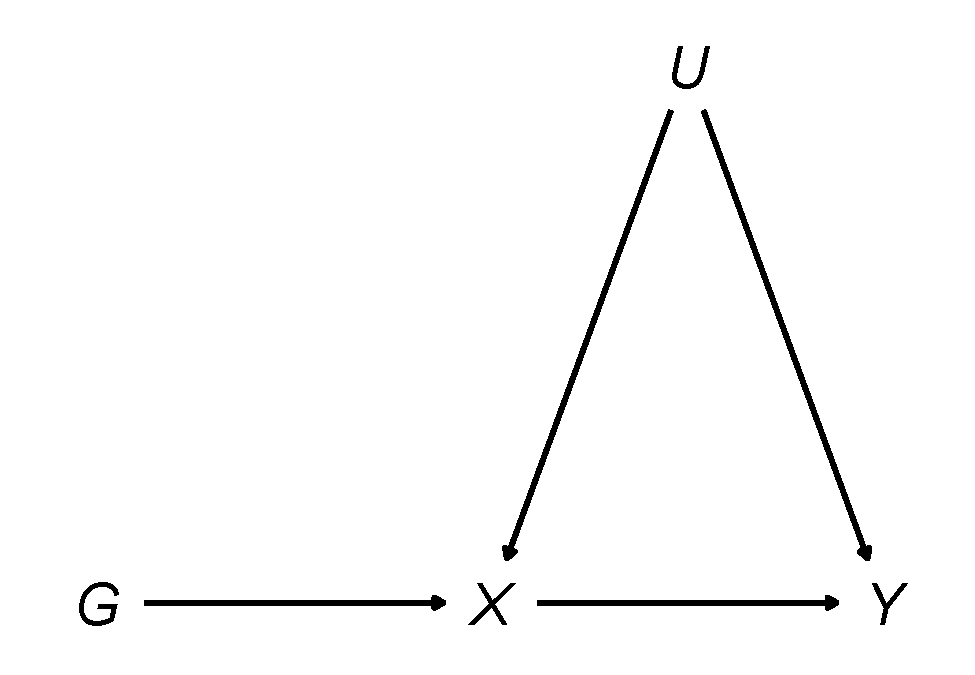
\includegraphics[keepaspectratio]{MSc_Thesis_Bookdown_files/figure-latex/DAG-base-plot-1.pdf}}

\begin{Shaded}
\begin{Highlighting}[]
\CommentTok{\# Formatting for assumption labels}
\NormalTok{assumption\_label\_col }\OtherTok{\textless{}{-}}\NormalTok{ edin\_muted\_blue\_hex}
\NormalTok{assumption\_label\_size }\OtherTok{\textless{}{-}} \DecValTok{4}
\NormalTok{assumption\_viol\_label\_col }\OtherTok{\textless{}{-}}\NormalTok{ edin\_burgundy\_hex}
\NormalTok{assumption\_viol\_label\_size }\OtherTok{\textless{}{-}} \DecValTok{4}
\NormalTok{assumption\_viol\_cross\_size }\OtherTok{\textless{}{-}} \DecValTok{6}

\CommentTok{\# Formatting for parameter labels}
\NormalTok{parameter\_label\_col }\OtherTok{\textless{}{-}}\NormalTok{ edin\_spruce\_grey\_hex}
\NormalTok{parameter\_label\_size }\OtherTok{\textless{}{-}} \DecValTok{5}

\CommentTok{\# parameter\_vals \textless{}{-} list(size = 4,}
\CommentTok{\#                        fontface = "italic", }
\CommentTok{\#                        colour = "red")}


\NormalTok{assumptions\_dag\_plot }\OtherTok{\textless{}{-}}\NormalTok{ base\_dag\_plot }\SpecialCharTok{+}
  \CommentTok{\# Line {-} Direct effects/uncorrelated pleiotropy/alpha, IV assumption 3}
  \FunctionTok{geom\_dag\_edges\_arc}\NormalTok{(}\FunctionTok{aes}\NormalTok{(}\AttributeTok{x =} \DecValTok{0}\NormalTok{,}
                         \AttributeTok{xend =} \DecValTok{2}\NormalTok{,}
                         \AttributeTok{y =} \FloatTok{0.5}\NormalTok{,}
                         \AttributeTok{yend =} \FloatTok{0.5}\NormalTok{,}
                         \AttributeTok{edge\_linetype =} \StringTok{"dotted"}\NormalTok{),}
                     \AttributeTok{curvature =} \SpecialCharTok{{-}}\FloatTok{0.4}\NormalTok{,}
                     \AttributeTok{arrow =}\NormalTok{ grid}\SpecialCharTok{::}\FunctionTok{arrow}\NormalTok{(}\AttributeTok{length =}\NormalTok{ grid}\SpecialCharTok{::}\FunctionTok{unit}\NormalTok{(}\DecValTok{12}\NormalTok{, }\StringTok{"pt"}\NormalTok{), }\AttributeTok{type =} \StringTok{"closed"}\NormalTok{)) }\SpecialCharTok{+}
  \CommentTok{\# Line {-} Direct effects on confounder/correlated pleiotropy, IV assumption 2}
  \FunctionTok{geom\_dag\_edges\_arc}\NormalTok{(}\FunctionTok{aes}\NormalTok{(}\AttributeTok{x =} \DecValTok{0}\NormalTok{,}
                         \AttributeTok{xend =} \FloatTok{1.5}\NormalTok{,}
                         \AttributeTok{y =} \FloatTok{0.5}\NormalTok{,}
                         \AttributeTok{yend =} \DecValTok{1}\NormalTok{,}
                         \AttributeTok{edge\_linetype =} \StringTok{"dotted"}\NormalTok{),}
                     \AttributeTok{curvature =} \FloatTok{0.3}\NormalTok{,}
                     \AttributeTok{arrow =}\NormalTok{ grid}\SpecialCharTok{::}\FunctionTok{arrow}\NormalTok{(}\AttributeTok{length =}\NormalTok{ grid}\SpecialCharTok{::}\FunctionTok{unit}\NormalTok{(}\DecValTok{12}\NormalTok{, }\StringTok{"pt"}\NormalTok{), }\AttributeTok{type =} \StringTok{"closed"}\NormalTok{)}
\NormalTok{                     ) }\SpecialCharTok{+}
  \CommentTok{\# \# Label {-} alpha}
  \CommentTok{\# geom\_dag\_text(x = 1, }
  \CommentTok{\#               y = 0.25, }
  \CommentTok{\#               label = "\textbackslash{}U03B1", }
  \CommentTok{\#               size = parameter\_label\_size,}
  \CommentTok{\#               fontface = "italic", }
  \CommentTok{\#               colour = parameter\_label\_col) +}
  \CommentTok{\# Label {-} beta}
  \FunctionTok{geom\_dag\_text}\NormalTok{(}\AttributeTok{x =} \FloatTok{1.5}\NormalTok{, }
                \AttributeTok{y =} \FloatTok{0.55}\NormalTok{, }
                \AttributeTok{label =} \FunctionTok{expression}\NormalTok{(beta), }\CommentTok{\#"\textbackslash{}U03B2",}
                \AttributeTok{size =}\NormalTok{ parameter\_label\_size,}
                \AttributeTok{fontface =} \StringTok{"italic"}\NormalTok{,}
                \AttributeTok{colour =}\NormalTok{ parameter\_label\_col}
\NormalTok{                ) }\SpecialCharTok{+}
  \CommentTok{\# Label {-} gamma (Y)}
  \FunctionTok{geom\_dag\_text}\NormalTok{(}\AttributeTok{x =} \FloatTok{0.5}\NormalTok{, }
                \AttributeTok{y =} \FloatTok{0.55}\NormalTok{, }
                \AttributeTok{label =} \FunctionTok{expression}\NormalTok{(gamma), }\CommentTok{\#"\textbackslash{}U03B3",}
                \AttributeTok{size =}\NormalTok{ parameter\_label\_size,}
                \AttributeTok{fontface =} \StringTok{"italic"}\NormalTok{,}
                \AttributeTok{colour =}\NormalTok{ parameter\_label\_col}
\NormalTok{                ) }\SpecialCharTok{+}
  \CommentTok{\# Label {-} Gamma (7)}
  \FunctionTok{geom\_dag\_text}\NormalTok{(}\AttributeTok{x =} \DecValTok{1}\NormalTok{, }
                \AttributeTok{y =} \FloatTok{0.001}\NormalTok{, }
                \AttributeTok{label =} \FunctionTok{expression}\NormalTok{(}\StringTok{"|{-} {-} {-} {-} {-} {-} {-} {-} {-} {-} {-} {-} {-} {-} {-} {-} {-} {-} {-}"}\SpecialCharTok{\textasciitilde{}}\NormalTok{Gamma}\SpecialCharTok{\textasciitilde{}} \StringTok{"="} \SpecialCharTok{\textasciitilde{}}\NormalTok{ gamma }\SpecialCharTok{*}\NormalTok{ beta}\SpecialCharTok{\textasciitilde{}}\StringTok{"{-} {-} {-} {-} {-} {-} {-} {-} {-} {-} {-} {-} {-} {-} {-} {-} {-} {-} {-}|"}\NormalTok{), }
                \CommentTok{\#label = expression("\textbackslash{}\textbackslash{}\textasciitilde{} \textasciitilde{} \textasciitilde{} \textasciitilde{} \textasciitilde{} \textasciitilde{} \textasciitilde{} \textasciitilde{} \textasciitilde{} \textasciitilde{} \textasciitilde{} \textasciitilde{} \textasciitilde{}"\textasciitilde{}Gamma\textasciitilde{} "=" \textasciitilde{} gamma * beta\textasciitilde{}"\textasciitilde{} \textasciitilde{} \textasciitilde{} \textasciitilde{} \textasciitilde{} \textasciitilde{} \textasciitilde{} \textasciitilde{} \textasciitilde{} \textasciitilde{} \textasciitilde{} \textasciitilde{} \textasciitilde{}/"), }
                \AttributeTok{size =}\NormalTok{ parameter\_label\_size,}
                \AttributeTok{fontface =} \StringTok{"italic"}\NormalTok{, }
                \AttributeTok{colour =}\NormalTok{ parameter\_label\_col) }\SpecialCharTok{+}
  \CommentTok{\# Label {-} IV1}
  \FunctionTok{geom\_dag\_text}\NormalTok{(}\AttributeTok{x =} \FloatTok{0.5}\NormalTok{, }
                \AttributeTok{y =} \FloatTok{0.45}\NormalTok{, }
                \AttributeTok{label =} \StringTok{"Assumption 1: Relevance"}\NormalTok{, }
                \AttributeTok{size =}\NormalTok{ assumption\_label\_size, }
                \AttributeTok{colour =}\NormalTok{ assumption\_label\_col) }\SpecialCharTok{+}
  \CommentTok{\# Label {-} IV2}
  \FunctionTok{geom\_dag\_text}\NormalTok{(}\AttributeTok{x =} \FloatTok{0.4}\NormalTok{, }
                \AttributeTok{y =} \FloatTok{1.05}\NormalTok{, }
                \AttributeTok{label =} \StringTok{"Assumption 2:}\SpecialCharTok{\textbackslash{}n}\StringTok{Independence"}\NormalTok{, }
                \AttributeTok{size =}\NormalTok{ assumption\_label\_size, }
                \AttributeTok{colour =}\NormalTok{ assumption\_label\_col) }\SpecialCharTok{+}
  \CommentTok{\# Cross {-} IV2}
  \FunctionTok{geom\_dag\_text}\NormalTok{(}\AttributeTok{x =} \FloatTok{0.65}\NormalTok{, }
                \AttributeTok{y =} \DecValTok{1}\NormalTok{, }
                \AttributeTok{label =} \StringTok{"X"}\NormalTok{, }
                \AttributeTok{size =}\NormalTok{ assumption\_viol\_cross\_size,}
                \AttributeTok{fontface =} \StringTok{"bold"}\NormalTok{, }
                \AttributeTok{colour =}\NormalTok{ assumption\_label\_col) }\SpecialCharTok{+}
  \CommentTok{\# Label {-} Correlated Pleiotropy}
  \FunctionTok{geom\_dag\_text}\NormalTok{(}\AttributeTok{x =} \FloatTok{0.85}\NormalTok{, }
                \AttributeTok{y =} \FloatTok{0.875}\NormalTok{, }
                \AttributeTok{label =} \StringTok{"Correlated Pleiotropy}\SpecialCharTok{\textbackslash{}n}\StringTok{(InSIDE Assumption Violated)"}\NormalTok{, }
                \AttributeTok{size =}\NormalTok{ assumption\_viol\_label\_size,}
                \CommentTok{\#fontface = "italic", }
                \AttributeTok{colour =}\NormalTok{ assumption\_viol\_label\_col) }\SpecialCharTok{+}
  \CommentTok{\# Label {-} IV3}
  \FunctionTok{geom\_dag\_text}\NormalTok{(}\AttributeTok{x =} \DecValTok{1}\NormalTok{, }
                \AttributeTok{y =} \FloatTok{0.16}\NormalTok{, }
                \AttributeTok{label =} \StringTok{"Assumption 3: Exclusion}\SpecialCharTok{\textbackslash{}n}\StringTok{Restriction"}\NormalTok{, }
                \AttributeTok{size =}\NormalTok{ assumption\_label\_size, }
                \AttributeTok{colour =}\NormalTok{ assumption\_label\_col) }\SpecialCharTok{+}
  \CommentTok{\# Cross {-} IV3}
  \FunctionTok{geom\_dag\_text}\NormalTok{(}\AttributeTok{x =} \DecValTok{1}\NormalTok{, }
                \AttributeTok{y =} \FloatTok{0.06}\NormalTok{, }
                \AttributeTok{label =} \StringTok{"X"}\NormalTok{, }
                \AttributeTok{size =}\NormalTok{ assumption\_viol\_cross\_size,}
                \AttributeTok{fontface =} \StringTok{"bold"}\NormalTok{, }
                \AttributeTok{colour =}\NormalTok{ assumption\_label\_col) }\SpecialCharTok{+}
  \CommentTok{\# Label {-} Uncorrelated Pleiotropy}
  \FunctionTok{geom\_dag\_text}\NormalTok{(}\AttributeTok{x =} \DecValTok{1}\NormalTok{, }
                \AttributeTok{y =} \FloatTok{0.27}\NormalTok{, }
                \AttributeTok{label =} \StringTok{"Uncorrelated Pleiotropy"}\NormalTok{, }
                \AttributeTok{size =}\NormalTok{ assumption\_viol\_label\_size,}
                \CommentTok{\#fontface = "italic", }
                \AttributeTok{colour =}\NormalTok{ assumption\_viol\_label\_col) }\CommentTok{\#+}
  \CommentTok{\#labs(\#title = "Key Assumptions in Mendelian Randomisation",}
       \CommentTok{\#subtitle = "", \#[@burgess\_sensitivity\_2016]}
       \CommentTok{\#caption = "\textbackslash{}nG: Genetic Instrument, U: Confounders, X: Exposure, Y: Outcome\textbackslash{}n" )}

\NormalTok{assumptions\_dag\_plot}
\end{Highlighting}
\end{Shaded}

\begin{figure}
\centering
\pandocbounded{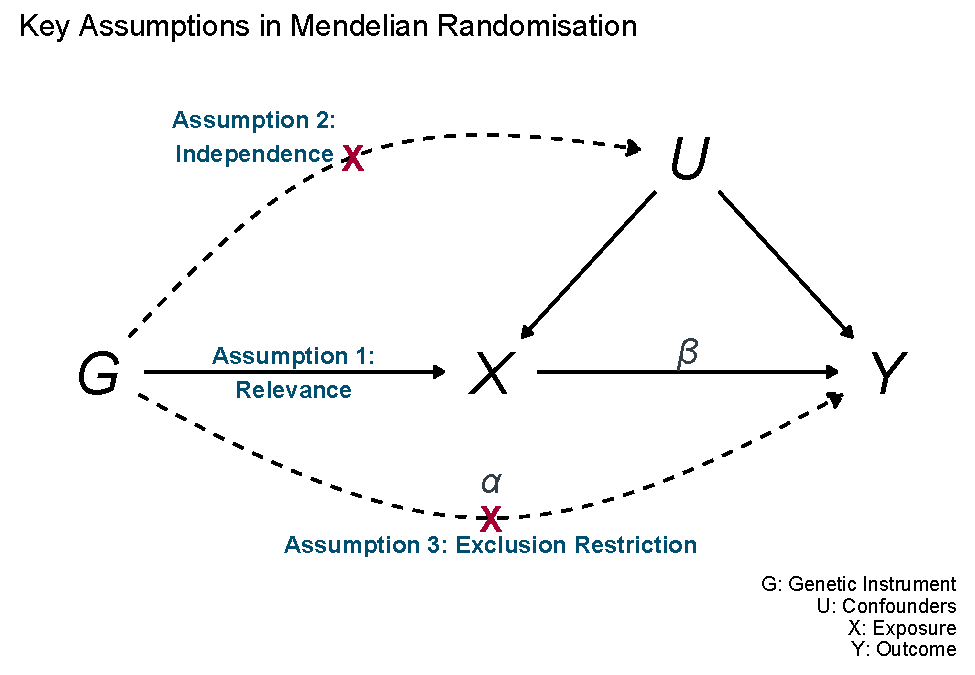
\includegraphics[keepaspectratio]{MSc_Thesis_Bookdown_files/figure-latex/DAG-assumptions-plot-1.pdf}}
\caption{\label{fig:DAG-assumptions-plot}Causal diagram illustrating the relationships between genetic instrument \emph{G}, exposure \emph{X}, outcome \emph{Y} and confounders of the exposure-outcome relationship \emph{U} in Mendelian randomisation studies. Blue text \& crosses represent key assumptions to ensure valid inference of causal effect of \emph{X} on \emph{Y} using \emph{G} as an instrumental variable. Red text represents violations of these assumptions that may lead to invalid inference through opening of alternate causal pathways. Greek characters represent the key parameters/association coefficients to be estimated. Adapted from Burgess et al 2016\textsuperscript{\citeproc{ref-burgess_sensitivity_2016}{7}}}
\end{figure}

Typically, \hyperref[acronyms_MR]{MR} studies estimate the causal effect using several genetic instruments; the causal effect estimate derived from the \(jth\) instrument is denoted \(\hat{\beta}_j\). Let:

\begin{equation} 
X|G_j = \gamma_0 + \gamma_j G_j + \epsilon_{X_j}
\end{equation}

\begin{equation} 
Y|G_j = \Gamma_0 + \Gamma_j G_j + \epsilon_{Y_j}
\end{equation}

be linear models for exposure and outcome, respectively, given a specific genetic instrument \(G_j\), where:

\begin{itemize}
\item
  \(\gamma_0\) and \(\Gamma_0\) reflect intercept values corresponding to the predicted value for \(X\) and \(Y\), respectively, when \(G_j = 0\) (i.e.~these are the predicted values for an individual carrying the non-effect allele of the genetic variant)
\item
  \(\gamma_j\) and \(\Gamma_j\) are coefficients of association with the genetic variant, representing the extent to which an effect allele of \(G_j\) will perturb the value of \(X\) or \(Y\) versus the non-effect allele
\item
  \(\epsilon_{X_j}\) and \(\epsilon_{Y_j}\) are error terms, representing effects of variables not explicitly included in the model, e.g.~confounders of the exposure-outcome relationship (\(U\) in the causal diagram), and genetic contributions outside of \(G_j\).
\end{itemize}

It can be shown that a simple causal effect estimate for the exposure on the outcome can be obtained from a single genetic instrument by the Wald method, dividing the coefficient of gene-outcome association by the coefficient of gene-exposure association, i.e.:

\begin{equation} 
\hat{\beta}_j = \frac {\hat{\Gamma}_j} {\hat{\gamma}_j}
\end{equation}

These coefficients of gene-exposure and gene-outcome association (\(\hat{\gamma}\) and \(\hat{\Gamma}\)) can be obtained from a \hyperref[acronyms_GWAS]{genome-wide association study (GWAS)}, which quantifies associations between small genetic variations - known as \hyperref[acronyms_SNP]{single nucleotide polymorphism (SNP)}s - and various phenotypes. Each genetic instrument selected from a \hyperref[acronyms_GWAS]{GWAS} may be valid or invalid, depending on it meeting the above assumptions. The overall causal effect estimate \(\hat{\beta}\) from any given \hyperref[acronyms_MR]{MR} method will typically seek to pool effect estimates from several instruments so as to minimise effects of any invalid instruments included, e.g.~by removing/down-weighting contributions of genetic instruments which might be violating one or more assumptions. This is equivalent to plotting all estimated coefficients of gene-outcome association (\(\bar{\Gamma}\)) versus all estimated coefficients of gene-exposure association (\(\bar{\gamma}\)) for the set of instruments, then using the gradient of a regression line through the points as the causal effect estimate \(\hat{\beta}\); picking an \hyperref[acronyms_MR]{MR} methodology is analogous to choosing the method to draw the line of best fit (Figure \ref{fig:Gamma-gamma-plot}). For binary outcomes, the coefficients of gene-outcome association (\(\bar{\Gamma}\)) are expressed as log odds ratios (\(log(OR)\)) for estimating the causal effect, and the causal effect estimate can be converted to an \hyperref[acronyms_OR]{odds ratio (OR)} through exponentiation, i.e.:

\begin{equation} 
OR = e^{\hat{\beta}}
\end{equation}

\begin{Shaded}
\begin{Highlighting}[]
\NormalTok{true\_beta }\OtherTok{\textless{}{-}} \FloatTok{0.25}

\CommentTok{\# Simulate individuals\textquotesingle{} data}
\NormalTok{causal\_data }\OtherTok{\textless{}{-}} \FunctionTok{get\_simulated\_MR\_data}\NormalTok{(}\AttributeTok{n\_participants =} \DecValTok{10000}\NormalTok{,}
                                     \AttributeTok{n\_instruments =} \DecValTok{25}\NormalTok{,}
                                     \AttributeTok{n\_datasets =} \DecValTok{1}\NormalTok{,}
                                     \AttributeTok{prop\_invalid =} \FloatTok{0.3}\NormalTok{,}
                                     \AttributeTok{causal\_effect =} \ConstantTok{TRUE}\NormalTok{, }
                                     \AttributeTok{beta\_val =}\NormalTok{ true\_beta, }
                                     \AttributeTok{balanced\_pleio =} \ConstantTok{FALSE}\NormalTok{)}

\CommentTok{\# Get models inc estimates of  Coeff\_G\_X/Coeff\_G\_Y}
\NormalTok{causal\_models }\OtherTok{\textless{}{-}} \FunctionTok{tibble}\NormalTok{(}\FunctionTok{get\_models}\NormalTok{(causal\_data)[[}\DecValTok{1}\NormalTok{]])}

\CommentTok{\# Assign values to vectors}
\NormalTok{coeff\_G\_X\_vect }\OtherTok{\textless{}{-}}\NormalTok{ causal\_models}\SpecialCharTok{$}\NormalTok{coeff\_G\_X}
\NormalTok{coeff\_G\_Y\_vect }\OtherTok{\textless{}{-}}\NormalTok{ causal\_models}\SpecialCharTok{$}\NormalTok{coeff\_G\_Y}
\NormalTok{coeff\_G\_X\_SE\_vect }\OtherTok{\textless{}{-}}\NormalTok{ causal\_models}\SpecialCharTok{$}\NormalTok{coeff\_G\_X\_SE}
\NormalTok{coeff\_G\_Y\_SE\_vect }\OtherTok{\textless{}{-}}\NormalTok{ causal\_models}\SpecialCharTok{$}\NormalTok{coeff\_G\_Y\_SE}


\CommentTok{\# Calculate WME estimates}
\NormalTok{causal\_models\_WME }\OtherTok{\textless{}{-}} \FunctionTok{mr\_weighted\_median}\NormalTok{(}\AttributeTok{b\_exp =}\NormalTok{ coeff\_G\_X\_vect,}
                                        \AttributeTok{b\_out =}\NormalTok{ coeff\_G\_Y\_vect,}
                                        \AttributeTok{se\_exp =}\NormalTok{ coeff\_G\_X\_SE\_vect,}
                                        \AttributeTok{se\_out =}\NormalTok{ coeff\_G\_Y\_SE\_vect,}
                                        \AttributeTok{parameters =} \FunctionTok{list}\NormalTok{(}\AttributeTok{nboot =} \DecValTok{1000}\NormalTok{)}
\NormalTok{                                        )}
\CommentTok{\# Calculate gradients for plotting}
\NormalTok{lm\_gradient }\OtherTok{\textless{}{-}} \FunctionTok{round}\NormalTok{(}\FunctionTok{coefficients}\NormalTok{(}\FunctionTok{lm}\NormalTok{(causal\_models}\SpecialCharTok{$}\NormalTok{coeff\_G\_Y }\SpecialCharTok{\textasciitilde{}} \DecValTok{0} \SpecialCharTok{+}\NormalTok{ causal\_models}\SpecialCharTok{$}\NormalTok{coeff\_G\_X)[}\DecValTok{1}\NormalTok{]), }\AttributeTok{digits =} \DecValTok{2}\NormalTok{)}

\NormalTok{WME\_gradient }\OtherTok{\textless{}{-}} \FunctionTok{round}\NormalTok{(causal\_models\_WME}\SpecialCharTok{$}\NormalTok{b, }\AttributeTok{digits =} \DecValTok{2}\NormalTok{)}

\CommentTok{\# Extra tibble for plotting}
\NormalTok{lines\_tib }\OtherTok{\textless{}{-}} \FunctionTok{tibble}\NormalTok{(}\AttributeTok{intercept =} \FunctionTok{c}\NormalTok{(}\DecValTok{0}\NormalTok{,}\DecValTok{0}\NormalTok{,}\DecValTok{0}\NormalTok{),}
                    \AttributeTok{slope =} \FunctionTok{c}\NormalTok{(true\_beta, lm\_gradient, WME\_gradient),}
                    \AttributeTok{values =} \FunctionTok{c}\NormalTok{(}\StringTok{"True"}\NormalTok{, }\StringTok{"Linear"}\NormalTok{, }\StringTok{"WME"}\NormalTok{)}
\NormalTok{                    )}

\CommentTok{\# Plot}
\NormalTok{Gamma\_gamma\_plot }\OtherTok{\textless{}{-}}\NormalTok{ causal\_models }\SpecialCharTok{\%\textgreater{}\%}
  \FunctionTok{mutate}\NormalTok{(}\AttributeTok{Invalid =}\NormalTok{ (alpha }\SpecialCharTok{!=} \DecValTok{0}\NormalTok{)) }\SpecialCharTok{\%\textgreater{}\%} 
  \FunctionTok{plot\_template}\NormalTok{() }\SpecialCharTok{+}
  \FunctionTok{aes}\NormalTok{(}\AttributeTok{x =}\NormalTok{ coeff\_G\_X, }
      \AttributeTok{y =}\NormalTok{ coeff\_G\_Y) }\SpecialCharTok{+} 
  \CommentTok{\# Instruments}
  \FunctionTok{geom\_point}\NormalTok{(}\FunctionTok{aes}\NormalTok{(}\AttributeTok{fill =}\NormalTok{ Invalid),}
             \AttributeTok{pch =} \DecValTok{21}\NormalTok{,}
             \CommentTok{\#alpha = 0.75,}
             \AttributeTok{size =} \DecValTok{3}\NormalTok{) }\SpecialCharTok{+}
  \CommentTok{\# Lines}
  \FunctionTok{geom\_abline}\NormalTok{(}\AttributeTok{data =}\NormalTok{ lines\_tib,}
              \FunctionTok{aes}\NormalTok{(}\AttributeTok{colour =}\NormalTok{ values,}
                  \AttributeTok{slope =}\NormalTok{ slope,}
                  \AttributeTok{intercept =}\NormalTok{ intercept),}
              \AttributeTok{size =} \FunctionTok{c}\NormalTok{(}\FloatTok{1.5}\NormalTok{, }\FloatTok{0.75}\NormalTok{, }\FloatTok{0.75}\NormalTok{)}
\NormalTok{              ) }\SpecialCharTok{+}
  \FunctionTok{scale\_colour\_manual}\NormalTok{(}\AttributeTok{name =} \StringTok{"Effect Estimate"}\NormalTok{,}
                      \AttributeTok{values =} \FunctionTok{c}\NormalTok{(}\StringTok{"True"} \OtherTok{=}\NormalTok{ edin\_spruce\_grey\_hex,}
                                 \StringTok{"Linear"} \OtherTok{=}\NormalTok{ edin\_bright\_blue\_hex,}
                                 \StringTok{"WME"} \OtherTok{=}\NormalTok{ edin\_bright\_pink\_hex),}
                      \AttributeTok{labels =} \FunctionTok{c}\NormalTok{(}\StringTok{"True"} \OtherTok{=} \StringTok{"True \textbackslash{}U03B2"}\NormalTok{, }
                                 \StringTok{"Linear"} \OtherTok{=} \StringTok{"Least Squares"}\NormalTok{,}
                                 \StringTok{"WME"} \OtherTok{=} \StringTok{"Weighted Median"}\NormalTok{),}
                      \AttributeTok{guide =} \StringTok{"legend"}\NormalTok{) }\SpecialCharTok{+}
  \CommentTok{\# Add betas}
  \DocumentationTok{\#\# True}
  \FunctionTok{geom\_text}\NormalTok{(}\AttributeTok{label =} \FunctionTok{paste0}\NormalTok{(}\StringTok{"True \textbackslash{}U03B2 = "}\NormalTok{, true\_beta), }\CommentTok{\#beta}
            \AttributeTok{x =} \FloatTok{0.08}\NormalTok{, }\CommentTok{\# labels with gradient (causal effect estimate)}
            \AttributeTok{y =} \FloatTok{0.01}\NormalTok{,}
            \AttributeTok{size =} \FloatTok{3.5}\NormalTok{, }
            \AttributeTok{fontface =} \StringTok{"italic"}\NormalTok{,}
            \AttributeTok{colour =}\NormalTok{ edin\_spruce\_grey\_hex, }
            \AttributeTok{hjust =} \DecValTok{0}\NormalTok{, }
            \AttributeTok{data =}\NormalTok{ . }\SpecialCharTok{\%\textgreater{}\%} \FunctionTok{slice\_head}\NormalTok{() }\CommentTok{\# prevent over{-}printing}
\NormalTok{  ) }\SpecialCharTok{+}
  \DocumentationTok{\#\# Linear}
  \FunctionTok{geom\_text}\NormalTok{(}\AttributeTok{label =} \FunctionTok{expression}\NormalTok{(}\StringTok{"Least Squares"} \SpecialCharTok{\textasciitilde{}} \FunctionTok{hat}\NormalTok{(beta) }\SpecialCharTok{\textasciitilde{}} \StringTok{"= 0.61"}\NormalTok{), }\CommentTok{\#beta}
            \AttributeTok{x =} \FloatTok{0.075}\NormalTok{, }\CommentTok{\# labels with gradient (causal effect estimate)}
            \AttributeTok{y =} \FloatTok{0.09}\NormalTok{,}
            \AttributeTok{size =} \FloatTok{3.5}\NormalTok{, }
            \CommentTok{\#fontface = "bold",}
            \AttributeTok{colour =}\NormalTok{ edin\_bright\_blue\_hex, }
            \AttributeTok{hjust =} \DecValTok{0}\NormalTok{, }
            \AttributeTok{data =}\NormalTok{ . }\SpecialCharTok{\%\textgreater{}\%} \FunctionTok{slice\_head}\NormalTok{() }\CommentTok{\# prevent over{-}printing}
\NormalTok{  ) }\SpecialCharTok{+}
  \DocumentationTok{\#\# WME}
  \FunctionTok{geom\_text}\NormalTok{(}\AttributeTok{label =} \FunctionTok{expression}\NormalTok{(}\StringTok{"WME"} \SpecialCharTok{\textasciitilde{}} \FunctionTok{hat}\NormalTok{(beta) }\SpecialCharTok{\textasciitilde{}} \StringTok{"= 0.3"}\NormalTok{), }\CommentTok{\#beta}
            \AttributeTok{x =} \FloatTok{0.088}\NormalTok{, }\CommentTok{\# labels with gradient (causal effect estimate)}
            \AttributeTok{y =} \FloatTok{0.045}\NormalTok{,}
            \AttributeTok{size =} \FloatTok{3.5}\NormalTok{, }
            \CommentTok{\#fontface = "bold",}
            \AttributeTok{colour =}\NormalTok{ edin\_bright\_pink\_hex, }
            \AttributeTok{hjust =} \DecValTok{0}\NormalTok{, }
            \AttributeTok{data =}\NormalTok{ . }\SpecialCharTok{\%\textgreater{}\%} \FunctionTok{slice\_head}\NormalTok{() }\CommentTok{\# prevent over{-}printing}
\NormalTok{  ) }\SpecialCharTok{+}
  \CommentTok{\# Colours for valid/invalid instruments}
  \FunctionTok{scale\_fill\_manual}\NormalTok{(}\AttributeTok{values =} \FunctionTok{c}\NormalTok{(edin\_muted\_turquoise\_hex, edin\_burgundy\_hex),}
                   \AttributeTok{labels =} \FunctionTok{c}\NormalTok{(}\StringTok{"Valid"}\NormalTok{, }\StringTok{"Invalid"}\NormalTok{)) }\SpecialCharTok{+}
  \CommentTok{\#Colours for regression lines}
  \FunctionTok{labs}\NormalTok{(}\CommentTok{\#title = plot\_title,}
    \CommentTok{\#x = "gene{-}exposure Coefficient ( \textbackslash{}U0302\textbackslash{}U03B3)",  \#U1D67 small gamma}
    \CommentTok{\#y = "gene{-}outcome Coefficient ( \textbackslash{}U0302\textbackslash{}U1D26)") + \#U0393 big Gamma}
    \AttributeTok{x =} \FunctionTok{expression}\NormalTok{(}\StringTok{"Gene{-}Exposure Coefficient ("} \SpecialCharTok{\textasciitilde{}}\FunctionTok{hat}\NormalTok{(gamma)}\SpecialCharTok{\textasciitilde{}} \StringTok{")"}\NormalTok{),  }
    \AttributeTok{y =} \FunctionTok{expression}\NormalTok{(}\StringTok{"Gene{-}Outcome Coefficient ("} \SpecialCharTok{\textasciitilde{}}\FunctionTok{hat}\NormalTok{(Gamma)}\SpecialCharTok{\textasciitilde{}} \StringTok{")"}\NormalTok{),}
    \AttributeTok{colour =} \StringTok{"Regression Lines"}\NormalTok{,}
    \AttributeTok{fill =} \StringTok{"Instruments"}\NormalTok{) }\SpecialCharTok{+}
  \CommentTok{\#guides(guide)}
  \FunctionTok{xlim}\NormalTok{(}\SpecialCharTok{{-}}\FloatTok{0.01}\NormalTok{, }\FloatTok{0.125}\NormalTok{)}
  
\NormalTok{Gamma\_gamma\_plot}
\end{Highlighting}
\end{Shaded}

\begin{figure}
\centering
\pandocbounded{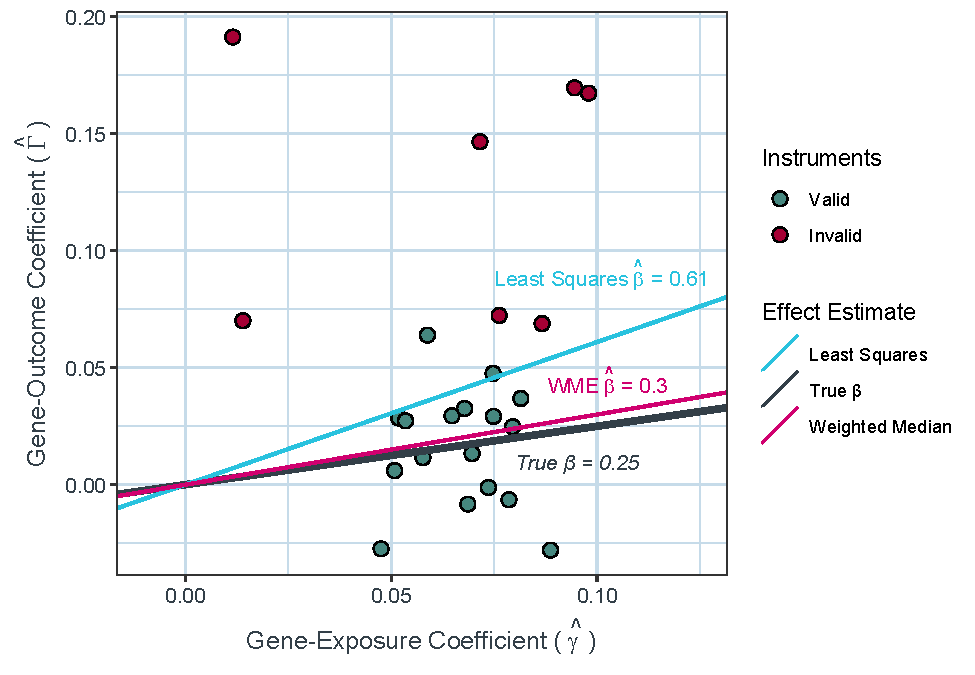
\includegraphics[keepaspectratio]{MSc_Thesis_Bookdown_files/figure-latex/Gamma-gamma-plot-1.pdf}}
\caption{\label{fig:Gamma-gamma-plot}Simulated MR Study on 10,000 individuals using 25 genetic instruments, of which 30\% are invalid (red points) and introduce directional pleiotropic effects. The true value of the exposure-outcome causal effect is 0.25 (grey line, causal effect represented by gradient). Regression using an unajusted least-squares linear model (light blue line) results in a biased estimate in the positive direction due to the influence of the invalid instruments. Using the Weighted Median Estimator method (pink line) attenuates the effects of the invalid instruments, resulting in an estimate closer to the true value. Adapted from Bowden et al 2016\textsuperscript{\citeproc{ref-bowden_consistent_2016}{8}}}
\end{figure}

\subsection{Violations to Assumptions}\label{violations-to-assumptions}

In practice, only the relevance assumption can be directly tested and proven. Typically, genetic variants for \hyperref[acronyms_MR]{MR} studies are selected as instruments based on their observed strength of association with exposures of interest in one or more \hyperref[acronyms_GWAS]{GWAS}. Sufficient gene-exposure association can be partly assured by selection using an appropriate genome-wide significance level (e.g.~\(p < 10 ^{-8}\)) during this instrument selection. Statistical testing can also further quantify the gene-exposure relationship; commonly used measures include the \(R^2\) statistic, representing the proportion of variance in the exposure explained by the genotype, and the related \(F\)-statistic, which additionally accounts for the sample size under investigation\textsuperscript{\citeproc{ref-richmond_mendelian_2022}{9}}. An \(F\)-statistic of \(\ge\) 10 is generally considered to represent a strong enough gene-exposure association to consider a genetic instrument for use\textsuperscript{\citeproc{ref-martens_instrumental_2006}{2}}.

The assumptions of independence and exclusion restriction depend on all determinants of the outcome, both known and unknown; as such, these can never be proven absolutely. Various methods have been proposed to quantify and account for violations of these two additional assumptions, including the weighted median estimator, described below\textsuperscript{\citeproc{ref-bowden_consistent_2016}{8}}.

The main methods to avoid violations of the independence assumption relate to appropriate controls for population structure, to avoid confounding due to ancestry or population stratification. For example, in two-sample MR studies, where gene-exposure and gene-outcome coefficients are estimated from two separate \hyperref[acronyms_GWAS]{GWAS} studies, spurious exposure-outcome associations can be generated by confounding due to underlying differences in e.g.~allele frequency, baseline disease risks etc. between ancestrally different populations; techniques such as principle components analysis can help control for such differences\textsuperscript{\citeproc{ref-richmond_mendelian_2022}{9}}.

Exclusion restriction is a particularly troublesome issue in MR, due to so-called (horizontal) genetic pleiotropy, which is abundant among genetic variants associated with disease traits\textsuperscript{\citeproc{ref-sivakumaran_abundant_2011}{10}}. A genetic variant has ``pleiotropic'' effects if it influences several traits simultaneously through its involvement in multiple biological pathways; such alternative biological pathways - and the resulting pleiotropic effects - are often unknown. Pleiotropic effects open unmeasured causal pathways between a genetic instrument and the outcome (Figure \ref{fig:DAG-assumptions-plot}), thus introducing bias in the \hyperref[acronyms_MR]{MR} estimate of the association between exposure and outcome. As pleiotropy influences outcome separate to the path involving the exposure of interest, the term ``direct effects'' is also used\textsuperscript{\citeproc{ref-hemani_evaluating_2018}{11}}. Where pleiotropic effects are in both positive and negative directions with a mean of zero - ``balanced pleiotropy'' - then they only add variance to the causal effect estimate, making inference more uncertain\textsuperscript{\citeproc{ref-morrison_mendelian_2020}{12}}. By contrast, ``directional pleiotropy'', where the mean of pleiotropic effects is non-zero, may introduce bias\textsuperscript{\citeproc{ref-bowden_consistent_2016}{8}} (Figure \ref{fig:Gamma-gamma-plot}). Note that, due to sampling error, the distribution of pleiotropic effects in a finite sample of genetic instruments may not reflect the true distribution across all possible genetic instruments for a given trait. For example, even where balanced pleiotropy is present across all genetic variants influencing a trait, bias could still be introduced into \hyperref[acronyms_MR]{MR} estimates of causal effect if a sample of instruments used happens (by chance) to have a non-zero mean pleiotropic effect on the outcome; the probability of this occuring reduces as the number of instruments used increases. In general, as the number of instruments used tends towards infinity, balanced pleiotropy will tend to introduce more variance than bias into causal effect estimates, and directional pleiotropy will tend to introduce bias more consistently than any additional variance it contributes.

If an additional causal pathway acts between gene \(G\) and outcome \(Y\) via a confounding factor \(U\), then the magnitude of direct - and therefore overall - effects of \(G\) on \(Y\) will correlate with the effects of \(G\) on \(X\) (i.e.~\(\Gamma \propto \gamma\)), and ``correlated pleiotropy'' is present. If an additional causal pathway acts directly between gene \(G\) and outcome \(Y\) independent of both exposure \(X\) and confounders \(U\), this results in ``uncorrelated pleiotropy'' (Figure \ref{fig:DAG-assumptions-plot}). Both correlated and uncorrelated pleiotropy can introduce bias which distorts the estimate of the true causal effect. In general, correlated pleiotropy is far more challenging to account for - potentially impossible using \hyperref[acronyms_MR]{MR} methods alone. Any attempt to statistically describe associations between genes, exposures and outcomes in the presence of correlated pleiotropy will struggle to identify a unique model - different parameterisations where different proportions of overall gene-outcome association are subsumed into the confounder-outcome association may be equally plausible given available observational data. For this reason, several MR methods explicitly require an additional assumption of \hyperref[acronyms_InSIDE]{Instrument Strength Independent of Direct Effect (InSIDE)}, i.e no correlated pleiotropy to be present\textsuperscript{\citeproc{ref-grant_bayesian_2024}{13}}.

\subsection{Weighted Median Estimator (WME)}\label{weighted-median-estimator-wme}

A common approach to produce exposure-outcome causal effect estimates robust to violations of the exclusion restriction assumption is the \hyperref[acronyms_WME]{weighted median estimator (WME)} method, proposed by Bowden et al\textsuperscript{\citeproc{ref-bowden_consistent_2016}{8}}.

In \hyperref[acronyms_WME]{WME} analysis, several genetic instruments are used to estimate the exposure-outcome causal effect \(\hat{\beta}\). Each instrument is known to be associated with the exposure of interest, but an unknown proportion of these instruments may be invalid due to pleiotropic genetic effects. The median causal effect will provide a consistent effect estimate despite presence of pleiotropic effects, provided that \textless50\% of included instruments are invalid. However, the simple median is an inefficient estimator - it weights estimates from all included instruments equally, without accounting for differences in precision of estimates obtained from each instrument, or by extension the factors influencing precision (e.g.~sample size)\textsuperscript{\citeproc{ref-bowden_consistent_2016}{8}}.

\hyperref[acronyms_WME]{WME} therefore assigns a weight to each genetic instrument's estimate of the causal effect according to the inverse of the variance of the estimate; these weighted effect estimates are used to construct a cumulative distribution function for the value of the causal effect across the range of values estimated based on each of the instruments. The 50th percentile of this distribution can then be taken as a ``weighted median estimate'' of the true causal effect, theoretically producing consistent causal estimates even if up to 50\% of the included information comes from invalid instruments\textsuperscript{\citeproc{ref-bowden_consistent_2016}{8}}. An example of \hyperref[acronyms_WME]{WME} attenuating the effects of invalid instruments is shown in Figure \ref{fig:Gamma-gamma-plot}.

\subsection{Issues With WME Confidence Intervals}\label{issues-with-wme-confidence-intervals}

\hyperref[acronyms_WME]{WME} calculation methods are available via several prolific \hyperref[acronyms_MR]{MR} tools: the R packages \texttt{MendelianRandomization}\textsuperscript{\citeproc{ref-yavorska_mendelianrandomization_2017}{14}} and \texttt{TwoSampleMR}, and the MR-Base web platform\textsuperscript{\citeproc{ref-hemani_mr-base_2018}{15}}. \hyperref[acronyms_WME]{WME} is now commonly used either as the primary method or as a sensitivity analysis to account for pleiotropic effects in a large number of \hyperref[acronyms_MR]{MR} studies. \hyperref[acronyms_WME]{WME}'s cited ``breakdown level'' of 50\% invalid instruments suggests that, in the vast majority of cases, \hyperref[acronyms_WME]{WME} causal effect estimates should be robust to the presence of pleiotropic effects\textsuperscript{\citeproc{ref-bowden_consistent_2016}{8}}. Despite this, a growing concern in the field of \hyperref[acronyms_MR]{MR} regarding high Type 1 error rates (i.e.~frequently declaring a causal effect between exposures and outcomes where none is actually present)\textsuperscript{\citeproc{ref-stender_reclaiming_2024}{16}}. If \hyperref[acronyms_WME]{WME} causal estimates are indeed robust to pleiotropy as claimed, another possible explanation for the method allowing null hypotheses to be falsely accepted would be if the \hyperref[acronyms_CI]{confidence interval (CI)} it reports for its causal estimates were inappropriately narrow.

\hyperref[acronyms_CI]{CI}s are a measure of the precision of an effect estimate, representing the range of values expected to contain the true effect given the observed variance of data around the observed average effect. Two key sources of uncertainty lead to variance in \hyperref[acronyms_MR]{MR} causal effect estimates:

\begin{enumerate}
\def\labelenumi{\arabic{enumi}.}
\item
  Uncertainty around estimation of the gene-exposure and gene-outcome coefficients (\(\hat{\gamma}\) and \(\hat{\Gamma}\)).
\item
  Uncertainty around the presence and magnitude of pleiotropic effects of included instruments.
\end{enumerate}

All commonly available tools to calculate \hyperref[acronyms_WME]{WME} implement the original method for generating the 95\% \hyperref[acronyms_CI]{CI}, using ``bootstrapping'' methodology to re-sample coefficients and causal estimates derived from each instrument. However, this approach only accounts for uncertainty from Point 1 (estimation of \(\hat{\gamma}\) and \(\hat{\Gamma}\)), and may therefore under-estimate the total variance relevant to causal effect estimation. A fuller explanation of the theoretical issues with this approach, together with an overview of bootstrapping in general, is presented in Appendix \ref{appendix-boot}.

In brief, this method would be expected to lead to \hyperref[acronyms_CI]{CI}s which are too narrow, giving over-confidence in the causal effect estimates obtained, and therefore inflated Type 1 error rates. Given the widespread use of \hyperref[acronyms_WME]{WME} across \hyperref[acronyms_MR]{MR} literature, this issue with its \hyperref[acronyms_CI]{CI} generation could potentially have far-reaching consequences.

\subsection{MR-Hevo}\label{mr-hevo}

MR-Hevo is an R package implementing an alternative approach to \hyperref[acronyms_MR]{MR} causal estimation. It uses Bayesian methodology to estimate MR causal effects and corresponding \hyperref[acronyms_CI]{CI}s.

In general, Bayesian methods can estimate parameters in the following way\textsuperscript{\citeproc{ref-clyde_chapter_2022}{17}}:

\begin{enumerate}
\def\labelenumi{\arabic{enumi}.}
\tightlist
\item
  A ``prior'' is specified - this is a probability distribution which represents existing beliefs about likely values of that parameter (e.g.~based on data from previous studies),
\item
  Further data is collected
\item
  The prior is updated based on the new data to form a ``posterior'' probability distribution, i.e.~an improved representation of likely values of the parameter is created which incorporates the new information available
\end{enumerate}

In this case, MR-Hevo directly addresses possible pleiotropy through use of a prior probability distribution which models pleiotropic effects of instruments on the outcome. The chosen prior distribution (a regularised hierarchical horseshoe, building on the work of Piironen \& Vehtari\textsuperscript{\citeproc{ref-piironen_sparsity_2017}{18}}) represents existing knowledge that most genetic instruments will not exert pleiotropic effects on the outcome, but some will, and these pleiotropic effects may be large. The R implementation of MR-Hevo then uses the probabilistic programming language, Stan, to directly sample the posterior probability distribution of pleiotropic effects on the outcome\textsuperscript{\citeproc{ref-mckeigue_inference_2024}{19}}. Essentially, this process involves using a computationally intensive, simulation based, ``trial-and-error'' approach using Markov chain Monte Carlo algorithms to perform inference over all model parameters and the available data\textsuperscript{\citeproc{ref-homan_no-u-turn_2014}{20},\citeproc{ref-hamra_markov_2013}{21}}.

Once the joint posterior distribution over all model parameters has been sampled, it is possible to obtain the marginal likelihood for the causal effect parameter given the data by dividing the posterior distributions by the prior. This computation marginalises over the pleiotropic effects, i.e.~integrates over all possible values for these effects, thus removing their influence on other model parameters. This approach accounts for both main sources of uncertainty in \hyperref[acronyms_MR]{MR} studies, and also allows classical hypothesis testing for the maximum likelihood estimate of the causal effect, including calculation of a p-value from the marginal likelihood\textsuperscript{\citeproc{ref-mckeigue_inference_2024}{19}}.

\subsection{Aims and Objectives}\label{aims-and-objectives}

The main aim of this study was to compare the outputs and resulting conclusions of MR-Hevo versus \hyperref[acronyms_WME]{WME} causal effect estimation methods in \hyperref[acronyms_MR]{MR} studies. In particular, this study aims to demonstrate if the \hyperref[acronyms_WME]{WME} approach gives over-confident causal estimates in the presence of pleiotropy, and whether this issue is more correctly handled by the MR-Hevo approach as its creators suggest. This will be achieved through addressing the research questions and objectives as outlined below:

\subsubsection*{Research Questions:}\label{research-questions}
\addcontentsline{toc}{subsubsection}{Research Questions:}

\begin{enumerate}
\def\labelenumi{\arabic{enumi}.}
\tightlist
\item
  How do \hyperref[acronyms_MR]{MR} causal effect estimates from MR-Hevo differ versus the weighted median estimator?
\item
  Do conclusions of existing MR studies using weighted median causal effect estimation change if MR-Hevo methods are used?
\end{enumerate}

\subsubsection*{Objectives:}\label{objectives}
\addcontentsline{toc}{subsubsection}{Objectives:}

\begin{enumerate}
\def\labelenumi{\arabic{enumi}.}
\tightlist
\item
  Quantify the bias of MR-Hevo causal estimates for simulated data under differing sets of common assumptions, with reference to the weighted median estimator
\item
  Quantify the variance of MR-Hevo causal estimates for simulated data under differing sets of common assumptions, with reference to the weighted median estimator
\item
  Compare the conclusions drawn from MR-Hevo causal effect estimation versus the weighted median estimator on real-world data
\end{enumerate}

\newpage

\section{Methods}\label{Methods}

\subsection{Simulation Study}\label{simulation-study}

To establish differences in \hyperref[acronyms_MR]{MR} causal estimates of MR-Hevo relative to WME, the bias and variance of estimates from both methods were evaluated using simulated datasets with known parameter values.

\subsubsection{Data Simulation}\label{data-simulation}

To aid comparability with existing methods and literature, the simulation methodology of the original WME exposition was reproduced based on published models and parameters in Appendix 3 of its supplementary materials\textsuperscript{\citeproc{ref-bowden_consistent_2016}{8}}. Full details of simulation reproduction, including code and validation of outputs, is presented in Appendix \ref{appendix-sim}.

In brief, simulations were created based on three different scenarios, each representing a common set of assumptions about underlying data used for MR. Each scenario poses an increasing challenge to valid inference using any given MR causal estimation methodology than the previous assumption set. Without loss of generality, all instruments are simulated to have a positive effect on the exposure:

\begin{enumerate}
\def\labelenumi{\arabic{enumi}.}
\item
  Balanced pleiotropy, InSIDE assumption satisfied - A proportion of invalid genetic instruments are present and introduce pleiotropic effects uncorrelated with the instrument strength. These pleiotropic effects were simulated from a uniform distribution centered around zero, and were equally likely to be positive as negative.
\item
  Directional pleiotropy, InSIDE assumption satisfied - A proportion of invalid genetic instruments are present and introduce pleiotropic effects on the outcome which are in the positive direction only. The magnitude of these pleiotropic effects on the outcome is uncorrelated with the magnitude of instrument effects on the exposure.
\item
  Directional pleiotropy, InSIDE assumption not satisfied - A proportion of invalid genetic instruments are present and introduce pleiotropic effects on the outcome which are in the positive direction only. The magnitude of these pleiotropic effects on the outcome is correlated with the magnitude of instrument effects on the exposure through action via a confounder.
\end{enumerate}

1,000 simulated datasets of participant-level data were generated for every combination of each scenario and each the following simulation parameters:

\begin{itemize}
\tightlist
\item
  Proportion of invalid instruments: 0\%, 10\%, 20\% or 30\%
\item
  Number of participants: \(n = 10,000\) or \(n = 20,000\)
\item
  Causal effect: null (\(\beta = 0\)) or positive (\(\beta = 0.1\))
\end{itemize}

The same 25 simulated genetic instruments were used across all datasets, with the status of each as valid/invalid determined by random draw per instrument at the start of each simulation run of 1,000 datasets.

Genotypes were simulated as for a two-sample setting: where number of particpants was \(n = 10,000\), then 20,000 genotypes were simulated - 10,000 for the cohort used to estimate gene-exposure association (\(\hat{\gamma}\)), and a separate cohort of 10,000 used to estimate gene-outcome association (\(\hat{\Gamma}\)). Parameter values for effect allele frequency were not specified by Bowden et al, though initial testing showed values around 0.5 produced WME causal effect estimates closest to published values when other parameters were matched\textsuperscript{\citeproc{ref-bowden_consistent_2016}{8}}. As such, effect allele frequencies were assigned per instrument from a uniform distribution between 0.4 to 0.6. Each effect allele freqency thus generated per instrument was then used as a probability to assign each simulated participant alleles for each instrument via two draws from a binomial distribution, such that each simulated participant had 0, 1 or 2 effect alleles for each instrument.

\subsubsection{Analysis of Simulated Data}\label{analysis-of-simulated-data}

Each dataset generated was analysed using both WME and MR-Hevo methods, via functions from the \texttt{TwoSampleMR} and \texttt{mrhevo} packages, respectively\textsuperscript{\citeproc{ref-hemani_mr-base_2018}{15},\citeproc{ref-mckeigue_inference_2024}{19}}. Results were aggregated per group of 1,000 simulated datasets corresponding to a particular combination of scenario and parameter values. The mean causal effect estimate, the mean standard errors/\hyperref[acronyms_CI]{CI}s of the causal effect estimate, and causality report rate (i.e.~percentage of simulated studies reported as a non-null causal effect, with a 95\% \hyperref[acronyms_CI]{CI} for the causal effect estimate not including 0) were reported for both \hyperref[acronyms_WME]{WME} and MR-Hevo for each combination of scenario/parameter values; these were computed over the 1,000 simulated \hyperref[acronyms_MR]{MR} studies using the same 25 genetic instruments in the same population.

Results of the above aggregations were tabulated as per Tables 2 \href{https://pmc.ncbi.nlm.nih.gov/articles/PMC4849733/table/gepi21965-tbl-0002/}{(link)} and 3\href{https://pmc.ncbi.nlm.nih.gov/articles/PMC4849733/table/gepi21965-tbl-0003/}{(link)} of Bowden et al\textsuperscript{\citeproc{ref-bowden_consistent_2016}{8}} to allow direct comparisons of the two methods versus each other and versus the published characteristics of other MR causal estimation methods evaluated by Bowden et al\textsuperscript{\citeproc{ref-bowden_consistent_2016}{8}}.

\subsection{Re-Analysis of Published Data}\label{re-analysis-of-published-data}

To investigate the potential implications of any differences in performance between WME and MR-Hevo methods, a selection of published studies reporting causal effect estimates using the WME method was re-analysed. A sample size of 10 published studies was pre-selected during study design as a pragmatic compromise between the scope of this project and the need to document frequency of any observed differences. In the original Bowden et al simulation studies, the WME causal estimation method was shown to generate a false-positive report rate of \(\ge\) 30\% with some parameter/scenario combinations\textsuperscript{\citeproc{ref-bowden_consistent_2016}{8}}. Therefore, even this relatively small sample of 10 studies could plausibly demonstrate differences between methods if sufficient instruments with pleiotropic effects are present in included studies, and if the MR-Hevo approach is as appropriately conservative as its creators propose.

In an attempt to characterise the greatest possible impact of using MR-Hevo instead of \hyperref[acronyms_WME]{WME} (and thus potentially controlling Type 1 error better), studies were chosen for re-analysis based on their number of citations in the wider MR literature. Compared to studies with few or no citations, highly-cited studies would be expected to have a larger impact on their respective fields if their conclusions were to change. In addition, highly-cited works will typically have been submitted to more scrutiny than less-cited works - both during peer review whilst under consideration by journals, and from the wider scientific community following the widespread dissemination evidenced by a high citation count. As such, it would be expected that highly-cited works are likely to be free of significant methodological flaws which may impede interpretation of any re-analysis.

\subsubsection{Citation Search}\label{citation-search}

The Scopus search platform\textsuperscript{\citeproc{ref-noauthor_scopus_nodate}{22}} was used on 15/04/2025 to retrieve all articles citing the original weighted median estimator exposition paper\textsuperscript{\citeproc{ref-bowden_consistent_2016}{8}}. The articles returned were sorted by the number of times each article itself had been cited, and the resulting list was saved to RIS format in blocks of ten articles for upload into the Covidence evidence synthesis platform\textsuperscript{\citeproc{ref-noauthor_covidence_2025}{23}}. Abstracts were screened by a single reviewer (B233241), starting with the most cited article and proceeding in descending order of citation count, against the following inclusion and exclusion criteria:

Inclusion criteria:

\begin{itemize}
\item
  Original two-sample MR study
\item
  Able to determine samples' ancestry sufficient to establish presence/potential degree of participant overlap between groups
\item
  Reporting \(\ge\) 20 human genetic instruments relating to exposure
\item
  Reports details of effect/non-effect alleles
\item
  Regression coefficients and standard errors and/or confidence intervals available for each genetic instrument used
\item
  Uses Weighted Median Estimator
\end{itemize}

Exclusion criteria:

\begin{itemize}
\item
  Methodology paper, review article, editorial or letter
\item
  English full-text not accessible
\end{itemize}

Where eligibility could not be determined from abstract screening alone, full texts were retrieved and screened against the same criteria. Screening of abstracts and full texts was undertaken in blocks of ten articles, until the target of ten included studies for reanalysis had been reached.

Where an article reported multiple exposure-outcome associations, data were only extracted for the association with the highest number of genetic instruments available, or else for the first reported association where several were based on the same number of instruments. Data were extracted from full texts of included studies using a standardised data collection template, which included publication details, citation count, primary study question, degree of potential participant overlap between groups, number/details of genetic instruments used, effect estimates/standard errors calculated, and conclusion regarding causality as determined by the weighted median estimator method.

\subsection{Data Manipulation and Analysis}\label{data-manipulation-and-analysis}

All simulations, data manipulations and data analyses were performed in R version 4.4.1 (2024-06-14 ucrt)\textsuperscript{\citeproc{ref-base}{24}}.

For the simulation study, full details of computation are available in Appendix \ref{appendix-sim}.

For citation search data, a standardised data collection form in Microsoft Excel\textsuperscript{\citeproc{ref-microsoft_corporation_microsoft_2018}{25}} was used to create .csv files for subsequent analysis in R; Excel's ``Get Data'' function was also used to extract tables of genetic instruments where these were presented in non-csv format (e.g.~pdf).

Data cleaning for citation search data was primarily undertaken using the Tidyverse suite of R packages\textsuperscript{\citeproc{ref-tidyverse}{26}}. A full list of packages used can be found in Appendix \ref{appendix-pkg}.

Data were manually screened at summary level and relevant features were extracted. Data were checked for completeness, consistency, duplicate values and plausibility. Data were transformed to an appropriate data type, and encoding of genetic variables was standardised into a single format. Instruments missing values for association coefficients and/or \hyperref[acronyms_SE]{standard error (SE)}s were excluded from the main analysis, and were imputed as the most extreme values per dataset as a sensitivity analysis. It was noted during early testing that causal effect estimation functions did not operate correctly in the presence of zero-value coefficients of genetic association and/or their standard errors; such zero values were therefore re-coded as an arbitrarily low value of \(10^{-100}\).

\subsection{Ethical Approval}\label{ethical-approval}

The protocol for this work has been reviewed and approved by the \hyperref[acronyms_UMREG]{Usher Masters Research Ethics Group (UMREG)} at the University of Edinburgh, Ethics ID: UM241126. Due to the nature of the project, using simulated and publically available data only, no significant ethical issues were foreseen, and sponsorship was deemed unnecessary by the \hyperref[acronyms_UMREG]{UMREG} reviewing panel.

\section{Results}\label{results-1}

\subsection{Simulation Study}\label{simulation-study-1}

\subsubsection{Data Simulation}\label{data-simulation-1}

Data were successfully simulated as intended. A selection of representative visualisations are presented in Figure \ref{fig:data-sim-validation}. Full details of testing used to validate model outputs from parameter inputs are given in Appendix \ref{appendix-sim-test}. The minimum \(F\)-statistic calculated from simulated instruments across all simulations was \textgreater10, indicating that instruments were sufficiently strongly associated with exposure to meet the relevance assumption of \hyperref[acronyms_IV]{IV} analysis (Tables \ref{tab:no-causal-sim-summ-display} and \ref{tab:causal-sim-summ-display}).

\begin{Shaded}
\begin{Highlighting}[]
\CommentTok{\# {-}{-}{-} Load data {-}{-}{-} \#}
\DocumentationTok{\#\# 0\% Invalid}
\NormalTok{no\_causal\_10k\_point0\_scen1\_models }\OtherTok{\textless{}{-}} \FunctionTok{readRDS}\NormalTok{(}\AttributeTok{file =} \FunctionTok{here}\NormalTok{(}\StringTok{"Data"}\NormalTok{, }\StringTok{"Simulated\_Datasets"}\NormalTok{, }\StringTok{"no\_causal\_10k\_point0\_scen1\_models.rds"}\NormalTok{))}
\NormalTok{causal\_10k\_point0\_scen1\_models }\OtherTok{\textless{}{-}} \FunctionTok{readRDS}\NormalTok{(}\AttributeTok{file =} \FunctionTok{here}\NormalTok{(}\StringTok{"Data"}\NormalTok{, }\StringTok{"Simulated\_Datasets"}\NormalTok{, }\StringTok{"causal\_10k\_point0\_scen1\_models.rds"}\NormalTok{))}

\DocumentationTok{\#\# 10\% Invalid}
\NormalTok{no\_causal\_10k\_point1\_scen1\_models }\OtherTok{\textless{}{-}} \FunctionTok{readRDS}\NormalTok{(}\AttributeTok{file =} \FunctionTok{here}\NormalTok{(}\StringTok{"Data"}\NormalTok{, }\StringTok{"Simulated\_Datasets"}\NormalTok{, }\StringTok{"no\_causal\_10k\_point1\_scen1\_models.rds"}\NormalTok{))}
\NormalTok{causal\_10k\_point1\_scen1\_models }\OtherTok{\textless{}{-}} \FunctionTok{readRDS}\NormalTok{(}\AttributeTok{file =} \FunctionTok{here}\NormalTok{(}\StringTok{"Data"}\NormalTok{, }\StringTok{"Simulated\_Datasets"}\NormalTok{, }\StringTok{"causal\_10k\_point1\_scen1\_models.rds"}\NormalTok{))}

\DocumentationTok{\#\# 20\% Invalid}
\NormalTok{no\_causal\_10k\_point2\_scen2\_models }\OtherTok{\textless{}{-}} \FunctionTok{readRDS}\NormalTok{(}\AttributeTok{file =} \FunctionTok{here}\NormalTok{(}\StringTok{"Data"}\NormalTok{, }\StringTok{"Simulated\_Datasets"}\NormalTok{, }\StringTok{"no\_causal\_10k\_point2\_scen2\_models.rds"}\NormalTok{))}
\NormalTok{causal\_10k\_point2\_scen2\_models }\OtherTok{\textless{}{-}} \FunctionTok{readRDS}\NormalTok{(}\AttributeTok{file =} \FunctionTok{here}\NormalTok{(}\StringTok{"Data"}\NormalTok{, }\StringTok{"Simulated\_Datasets"}\NormalTok{, }\StringTok{"causal\_10k\_point2\_scen2\_models.rds"}\NormalTok{))}

\DocumentationTok{\#\# 30\% Invalid}
\NormalTok{no\_causal\_10k\_point3\_scen3\_models }\OtherTok{\textless{}{-}} \FunctionTok{readRDS}\NormalTok{(}\AttributeTok{file =} \FunctionTok{here}\NormalTok{(}\StringTok{"Data"}\NormalTok{, }\StringTok{"Simulated\_Datasets"}\NormalTok{, }\StringTok{"no\_causal\_10k\_point3\_scen3\_models.rds"}\NormalTok{))}
\NormalTok{causal\_10k\_point3\_scen3\_models }\OtherTok{\textless{}{-}} \FunctionTok{readRDS}\NormalTok{(}\AttributeTok{file =} \FunctionTok{here}\NormalTok{(}\StringTok{"Data"}\NormalTok{, }\StringTok{"Simulated\_Datasets"}\NormalTok{, }\StringTok{"causal\_10k\_point3\_scen3\_models.rds"}\NormalTok{))}


\CommentTok{\# {-}{-}{-} Citation Search {-}{-}{-} \# }

\NormalTok{Citations\_Instrument\_Data }\OtherTok{\textless{}{-}} \FunctionTok{read.csv}\NormalTok{(}\FunctionTok{here}\NormalTok{(}\StringTok{"Data"}\NormalTok{, }\StringTok{"Citations\_Datasets"}\NormalTok{, }\StringTok{"Citations\_Instrument\_Data.csv"}\NormalTok{)) }\SpecialCharTok{\%\textgreater{}\%} \FunctionTok{as\_tibble}\NormalTok{() }\CommentTok{\#\%\textgreater{}\% filter(Instrument !="rs7326482") \%\textgreater{}\% mutate(N=1)}
\CommentTok{\# Citations\_Instrument\_Data\_2 \textless{}{-} read.csv(here("Data", "Citations\_Datasets", "Citations\_Instrument\_Data.csv")) \%\textgreater{}\% as.tibble() \#\%\textgreater{}\%filter(Instrument !="rs7326482") \%\textgreater{}\%  mutate(N=2)}
\end{Highlighting}
\end{Shaded}

\begin{Shaded}
\begin{Highlighting}[]
\CommentTok{\# Get random dataset index}
\FunctionTok{set.seed}\NormalTok{(}\DecValTok{1701}\NormalTok{)}
\NormalTok{rand\_example }\OtherTok{\textless{}{-}} \FunctionTok{sample}\NormalTok{(}\DecValTok{1}\SpecialCharTok{:}\DecValTok{1000}\NormalTok{, }\DecValTok{1}\NormalTok{, }\AttributeTok{replace =} \ConstantTok{FALSE}\NormalTok{)}

\CommentTok{\# Select random dataset from each scenario}
\NormalTok{models\_list }\OtherTok{\textless{}{-}} \FunctionTok{list}\NormalTok{(}
  \CommentTok{\# 0\% Invalid}
\NormalTok{  no\_causal\_10k\_point0\_scen1\_models[[rand\_example]],}
\NormalTok{  causal\_10k\_point0\_scen1\_models[[rand\_example]],}
  \DocumentationTok{\#\# 10\% Invalid}
\NormalTok{  no\_causal\_10k\_point1\_scen1\_models[[rand\_example]],}
\NormalTok{  causal\_10k\_point1\_scen1\_models[[rand\_example]],}
  \DocumentationTok{\#\# 20\% Invalid}
\NormalTok{  no\_causal\_10k\_point2\_scen2\_models[[rand\_example]],}
\NormalTok{  causal\_10k\_point2\_scen2\_models[[rand\_example]],}
  \DocumentationTok{\#\# 30\% Invalid}
\NormalTok{  no\_causal\_10k\_point3\_scen3\_models[[rand\_example]],}
\NormalTok{  causal\_10k\_point3\_scen3\_models[[rand\_example]]}
\NormalTok{)}

\CommentTok{\# Create blank list to receive plots}
\NormalTok{Gamma\_gamma\_plots }\OtherTok{\textless{}{-}} \FunctionTok{as.list}\NormalTok{(}\FunctionTok{rep}\NormalTok{(}\ConstantTok{NA}\NormalTok{, }\FunctionTok{length}\NormalTok{(models\_list)))}

\CommentTok{\# Create plot subtitles}
\NormalTok{subtitles }\OtherTok{\textless{}{-}} \FunctionTok{c}\NormalTok{(}
  \StringTok{"0\% Invalid"}\NormalTok{,}
  \StringTok{""}\NormalTok{,}
  \StringTok{"10\% Invalid, Scenario 1"}\NormalTok{,}
  \StringTok{""}\NormalTok{,}
  \StringTok{"20\% Invalid, Scenario 2"}\NormalTok{,}
  \StringTok{""}\NormalTok{,}
  \StringTok{"30\% Invalid, Scenario 3"}\NormalTok{,}
  \StringTok{""}
\NormalTok{)}


\CommentTok{\# Create plots}
\ControlFlowTok{for}\NormalTok{(model }\ControlFlowTok{in} \DecValTok{1}\SpecialCharTok{:}\FunctionTok{length}\NormalTok{(models\_list))\{}
  
  \CommentTok{\# Set beta for graph slope}
\NormalTok{  true\_beta }\OtherTok{\textless{}{-}} \FunctionTok{if\_else}\NormalTok{(model}\SpecialCharTok{\%\%}\DecValTok{2} \SpecialCharTok{==} \DecValTok{1}\NormalTok{,}
                       \AttributeTok{true =} \DecValTok{0}\NormalTok{,}
                       \AttributeTok{false =} \FloatTok{0.1}\NormalTok{) }
  
  \CommentTok{\# Label only left/bottom axes}
\NormalTok{  y\_lab }\OtherTok{\textless{}{-}} \FunctionTok{if\_else}\NormalTok{(model}\SpecialCharTok{\%\%}\DecValTok{2} \SpecialCharTok{==} \DecValTok{1}\NormalTok{,}
                   \AttributeTok{true =} \StringTok{"Gene{-}Outcome}\SpecialCharTok{\textbackslash{}n}\StringTok{Coefficient (\textbackslash{}U1D26)"}\NormalTok{,}
                   \AttributeTok{false =} \StringTok{""}\NormalTok{) }
  
\NormalTok{  x\_lab }\OtherTok{\textless{}{-}} \FunctionTok{case\_when}\NormalTok{(model }\SpecialCharTok{==} \FunctionTok{length}\NormalTok{(models\_list) }\SpecialCharTok{{-}} \DecValTok{1} \SpecialCharTok{|}\NormalTok{ model }\SpecialCharTok{==} \FunctionTok{length}\NormalTok{(models\_list) }\SpecialCharTok{\textasciitilde{}} \StringTok{"Gene{-}Exposure Coefficient (\textbackslash{}U03B3)"}\NormalTok{,}
                     \AttributeTok{.default =} \StringTok{""}\NormalTok{) }
  
  \CommentTok{\# Title Causal/Non{-}Causal}
\NormalTok{  causal\_title }\OtherTok{\textless{}{-}} \FunctionTok{case\_when}\NormalTok{(model }\SpecialCharTok{==}  \DecValTok{1} \SpecialCharTok{\textasciitilde{}} \StringTok{"No Causal Effect"}\NormalTok{,}
\NormalTok{                            model }\SpecialCharTok{==} \DecValTok{2} \SpecialCharTok{\textasciitilde{}} \StringTok{"Causal Effect"}\NormalTok{,}
                            \AttributeTok{.default =} \StringTok{""}\NormalTok{) }
  
  \CommentTok{\# Tag index}
\NormalTok{  tag\_index }\OtherTok{\textless{}{-}} \FunctionTok{if\_else}\NormalTok{(model}\SpecialCharTok{\%\%}\DecValTok{2} \SpecialCharTok{==} \DecValTok{1}\NormalTok{,}
                       \AttributeTok{true =}\NormalTok{ (model}\SpecialCharTok{+}\DecValTok{1}\NormalTok{)}\SpecialCharTok{/}\DecValTok{2}\NormalTok{,}
                       \AttributeTok{false =} \ConstantTok{FALSE}\NormalTok{) }
  
  \CommentTok{\# Tag text}
\NormalTok{  tag\_text }\OtherTok{\textless{}{-}} \FunctionTok{if\_else}\NormalTok{(model}\SpecialCharTok{\%\%}\DecValTok{2} \SpecialCharTok{==} \DecValTok{1}\NormalTok{,}
                       \AttributeTok{true =} \FunctionTok{paste0}\NormalTok{(letters[tag\_index], }\StringTok{")"}\NormalTok{),}
                       \AttributeTok{false =} \StringTok{""}\NormalTok{) }
  
  
  \CommentTok{\# Plot outline}
\NormalTok{  Gamma\_gamma\_plots[[model]] }\OtherTok{\textless{}{-}}\NormalTok{ models\_list[[model]] }\SpecialCharTok{\%\textgreater{}\%}
    \FunctionTok{tibble}\NormalTok{() }\SpecialCharTok{\%\textgreater{}\%} 
    \FunctionTok{mutate}\NormalTok{(}\AttributeTok{Invalid =}\NormalTok{ (alpha }\SpecialCharTok{!=} \DecValTok{0}\NormalTok{)) }\SpecialCharTok{\%\textgreater{}\%}
    \FunctionTok{plot\_template}\NormalTok{() }\SpecialCharTok{+}
    \FunctionTok{aes}\NormalTok{(}\AttributeTok{x =}\NormalTok{ coeff\_G\_X,}
        \AttributeTok{y =}\NormalTok{ coeff\_G\_Y) }\SpecialCharTok{+}
    \CommentTok{\# Instruments}
    \FunctionTok{geom\_point}\NormalTok{(}\FunctionTok{aes}\NormalTok{(}\AttributeTok{fill =}\NormalTok{ Invalid),}
               \AttributeTok{pch =} \DecValTok{21}\NormalTok{,}
               \AttributeTok{alpha =} \FloatTok{0.75}\NormalTok{,}
               \AttributeTok{size =} \DecValTok{3}\NormalTok{) }\SpecialCharTok{+}
    \CommentTok{\# Lines}
    \FunctionTok{geom\_abline}\NormalTok{(}\AttributeTok{colour =}\NormalTok{ edin\_uni\_blue\_hex,}
                \AttributeTok{slope =}\NormalTok{ true\_beta,}
                \AttributeTok{intercept =} \DecValTok{0}\NormalTok{,}
                \AttributeTok{size =} \DecValTok{1}\NormalTok{) }\SpecialCharTok{+}
    
    \CommentTok{\# Add betas}
    \DocumentationTok{\#\# True}
    \FunctionTok{geom\_text}\NormalTok{(}\AttributeTok{label =} \FunctionTok{paste0}\NormalTok{(}\StringTok{"True \textbackslash{}U03B2 = "}\NormalTok{, true\_beta), }\CommentTok{\#beta}
              \AttributeTok{x =} \FloatTok{0.1}\NormalTok{, }\CommentTok{\# labels with gradient (causal effect estimate)}
              \AttributeTok{y =} \SpecialCharTok{{-}}\FloatTok{0.1}\NormalTok{,}
              \AttributeTok{size =} \DecValTok{3}\NormalTok{,}
              \AttributeTok{fontface =} \StringTok{"italic"}\NormalTok{,}
              \AttributeTok{colour =}\NormalTok{ edin\_uni\_blue\_hex,}
              \AttributeTok{hjust =} \DecValTok{0}\NormalTok{,}
              \AttributeTok{data =}\NormalTok{ . }\SpecialCharTok{\%\textgreater{}\%} \FunctionTok{slice\_head}\NormalTok{() }\CommentTok{\# prevent over{-}printing}
\NormalTok{    ) }\SpecialCharTok{+}
    \CommentTok{\# Colours for valid/invalid instruments}
    \FunctionTok{scale\_fill\_manual}\NormalTok{(}\AttributeTok{values =} \FunctionTok{c}\NormalTok{(edin\_muted\_turquoise\_hex, edin\_burgundy\_hex),}
                      \AttributeTok{labels =} \FunctionTok{c}\NormalTok{(}\StringTok{"Valid"}\NormalTok{, }\StringTok{"Invalid"}\NormalTok{),}
                      \AttributeTok{guide =} \StringTok{"legend"}\NormalTok{,}
                      \AttributeTok{name =} \StringTok{"Instruments"}\NormalTok{) }\SpecialCharTok{+}
    \CommentTok{\# Labels}
    \FunctionTok{labs}\NormalTok{(}\CommentTok{\#title = causal\_title,}
         \AttributeTok{subtitle =}\NormalTok{ subtitles[model],}
         \AttributeTok{tag =}\NormalTok{ tag\_text,}
         \AttributeTok{x =}\NormalTok{ x\_lab,}
         \AttributeTok{y =}\NormalTok{ y\_lab) }\SpecialCharTok{+}
    \FunctionTok{theme}\NormalTok{(}\AttributeTok{legend.position =} \StringTok{"none"}\NormalTok{,}
          \AttributeTok{plot.margin =} \FunctionTok{unit}\NormalTok{(}\FunctionTok{c}\NormalTok{(}\FloatTok{0.1}\NormalTok{,}\FloatTok{0.1}\NormalTok{,}\FloatTok{0.1}\NormalTok{,}\FloatTok{0.1}\NormalTok{), }\StringTok{"cm"}\NormalTok{),}
          \AttributeTok{axis.text =} \FunctionTok{element\_text}\NormalTok{(}\AttributeTok{size =} \DecValTok{6}\NormalTok{), }
          \AttributeTok{axis.title =} \FunctionTok{element\_text}\NormalTok{(}\AttributeTok{size =} \DecValTok{7}\NormalTok{), }
          \AttributeTok{subtitle =} \FunctionTok{element\_text}\NormalTok{(}\AttributeTok{size =} \DecValTok{6}\NormalTok{)}
\NormalTok{          ) }\SpecialCharTok{+}
    \FunctionTok{xlim}\NormalTok{(}\SpecialCharTok{{-}}\FloatTok{0.06}\NormalTok{, }\FloatTok{0.2125}\NormalTok{) }\SpecialCharTok{+}
    \FunctionTok{ylim}\NormalTok{(}\SpecialCharTok{{-}}\FloatTok{0.11}\NormalTok{, }\FloatTok{0.25}\NormalTok{) }
  
\NormalTok{\}}

\CommentTok{\#Legend}
\NormalTok{legend }\OtherTok{\textless{}{-}} \FunctionTok{get\_legend}\NormalTok{(Gamma\_gamma\_plots[[}\FunctionTok{length}\NormalTok{(models\_list)]] }\SpecialCharTok{+}
                       \FunctionTok{theme}\NormalTok{(}\AttributeTok{legend.position =} \StringTok{"right"}\NormalTok{)}
\NormalTok{                     )}

\NormalTok{plot\_two\_cols }\OtherTok{\textless{}{-}} \FunctionTok{plot\_grid}\NormalTok{(}\AttributeTok{plotlist =}\NormalTok{ Gamma\_gamma\_plots, }
                           \AttributeTok{rel\_widths =} \FunctionTok{c}\NormalTok{(}\FloatTok{0.55}\NormalTok{, }\FloatTok{0.45}\NormalTok{),}
                           \AttributeTok{ncol =} \DecValTok{2}\NormalTok{)}


\CommentTok{\# Plot all}
\FunctionTok{plot\_grid}\NormalTok{(plot\_two\_cols,}
\NormalTok{          legend,}
          \AttributeTok{ncol =} \DecValTok{2}\NormalTok{,}
          \AttributeTok{rel\_widths =} \FunctionTok{c}\NormalTok{(}\DecValTok{1}\NormalTok{, }\FloatTok{0.2}\NormalTok{))}
\end{Highlighting}
\end{Shaded}

\begin{figure}
\centering
\pandocbounded{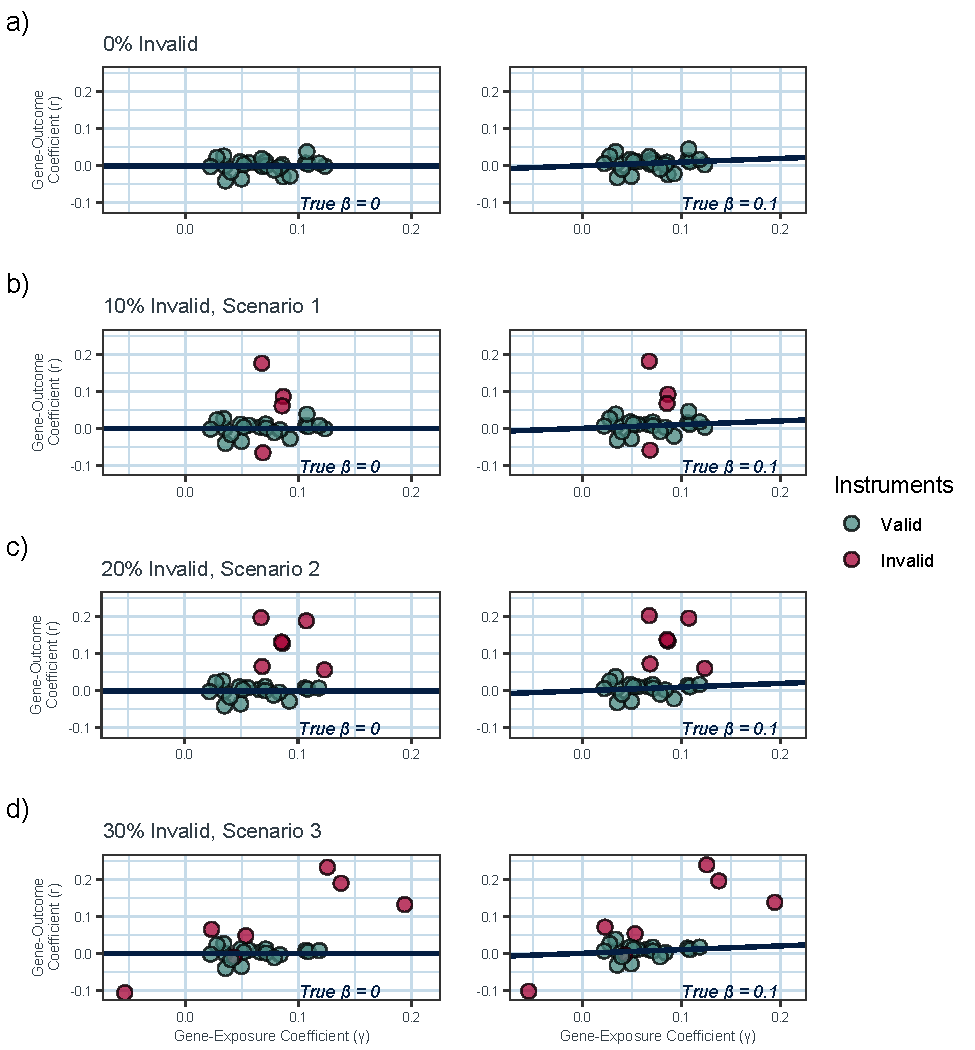
\includegraphics[keepaspectratio]{MSc_Thesis_Bookdown_files/figure-latex/data-sim-validation-1.pdf}}
\caption{\label{fig:data-sim-validation}Plots of a representative group of simulated datasets; all simulate genetic instruments from the same index from the same random seed. Left and right columns demonstrate null and positive true causal effects, respectively; the true causal effect is represented by the gradient of the line shown. The scenario and the proportion of invalid (i.e.~pleiotropic) genetic instruments changes with each row. a) 0\% of instruments invalid, rendering scenario assumptions regarding invalid assumptions irrelevant. b) 10\% of instruments invalid, Scenario 1: balanced pleiotropy simulated, though random sampling of these instruments has introduced some directionality; both variance and some bias are introduced to causal effect estimation. c) 20\% of instruments invalid, Scenario 2: directional pleiotropy biases in the direction of the invalid instruments. d) 30\% of instruments invalid, Scenario 3: directional pleiotropy and InSIDE assumption violation strongly biases towards a positive effect estimate in a manner difficult to statistically distinguish from a true causal effect.}
\end{figure}

\subsubsection{Analysis of Simulated Data}\label{analysis-of-simulated-data-1}

Due to a coding issue with outputs from MR-Hevo functions, the \hyperref[acronyms_SE]{SE}s for MR-Hevo causal estimates were not successfully retrieved; all 95\% \hyperref[acronyms_CI]{CI}s were retrieved as intended. To aid comprehension and comparison of below results with regards to variance of causal effect estimates, it was decided to display an estimated \hyperref[acronyms_SE]{SE} for MR-Hevo. Estimated \hyperref[acronyms_SE]{SE} was calculated as \((Upper \space CI - Lower \space CI) \div (2 \times 1.96)\), i.e.~approximating the bootstrap distribution as normally distributed per the expectation from \hyperref[acronyms_CLT]{central limit theorem (CLT)} (see Appendix \ref{appendix-boot}). However, the reader should note that, whilst reported MR-Hevo \hyperref[acronyms_CI]{CI}s are accurate, MR-Hevo \hyperref[acronyms_SE]{SE}s are approximate only.

\begin{Shaded}
\begin{Highlighting}[]
\CommentTok{\# {-}{-}{-} Load results {-}{-}{-} \#}
\CommentTok{\# No Causal:}
\NormalTok{no\_causal\_10k\_scen1\_sim\_summ\_tib }\OtherTok{\textless{}{-}} \FunctionTok{readRDS}\NormalTok{(}\AttributeTok{file =} \FunctionTok{here}\NormalTok{(}\StringTok{"Data"}\NormalTok{, }\StringTok{"Summary\_Tables"}\NormalTok{, }\StringTok{"no\_causal\_10k\_scen1\_sim\_summ\_tib.rds"}\NormalTok{))}
\NormalTok{no\_causal\_20k\_scen1\_sim\_summ\_tib }\OtherTok{\textless{}{-}} \FunctionTok{readRDS}\NormalTok{(}\AttributeTok{file =} \FunctionTok{here}\NormalTok{(}\StringTok{"Data"}\NormalTok{, }\StringTok{"Summary\_Tables"}\NormalTok{, }\StringTok{"no\_causal\_20k\_scen1\_sim\_summ\_tib.rds"}\NormalTok{))}

\NormalTok{no\_causal\_10k\_scen2\_sim\_summ\_tib }\OtherTok{\textless{}{-}} \FunctionTok{readRDS}\NormalTok{(}\AttributeTok{file =} \FunctionTok{here}\NormalTok{(}\StringTok{"Data"}\NormalTok{, }\StringTok{"Summary\_Tables"}\NormalTok{, }\StringTok{"no\_causal\_10k\_scen2\_sim\_summ\_tib.rds"}\NormalTok{))}
\NormalTok{no\_causal\_20k\_scen2\_sim\_summ\_tib }\OtherTok{\textless{}{-}} \FunctionTok{readRDS}\NormalTok{(}\AttributeTok{file =} \FunctionTok{here}\NormalTok{(}\StringTok{"Data"}\NormalTok{, }\StringTok{"Summary\_Tables"}\NormalTok{, }\StringTok{"no\_causal\_20k\_scen2\_sim\_summ\_tib.rds"}\NormalTok{))}

\NormalTok{no\_causal\_10k\_scen3\_sim\_summ\_tib }\OtherTok{\textless{}{-}} \FunctionTok{readRDS}\NormalTok{(}\AttributeTok{file =} \FunctionTok{here}\NormalTok{(}\StringTok{"Data"}\NormalTok{, }\StringTok{"Summary\_Tables"}\NormalTok{, }\StringTok{"no\_causal\_10k\_scen3\_sim\_summ\_tib.rds"}\NormalTok{))}
\NormalTok{no\_causal\_20k\_scen3\_sim\_summ\_tib }\OtherTok{\textless{}{-}} \FunctionTok{readRDS}\NormalTok{(}\AttributeTok{file =} \FunctionTok{here}\NormalTok{(}\StringTok{"Data"}\NormalTok{, }\StringTok{"Summary\_Tables"}\NormalTok{, }\StringTok{"no\_causal\_20k\_scen3\_sim\_summ\_tib.rds"}\NormalTok{))}


\CommentTok{\# Causal:}
\NormalTok{causal\_10k\_scen1\_sim\_summ\_tib }\OtherTok{\textless{}{-}} \FunctionTok{readRDS}\NormalTok{(}\AttributeTok{file =} \FunctionTok{here}\NormalTok{(}\StringTok{"Data"}\NormalTok{, }\StringTok{"Summary\_Tables"}\NormalTok{, }\StringTok{"causal\_10k\_scen1\_sim\_summ\_tib.rds"}\NormalTok{))}
\NormalTok{causal\_20k\_scen1\_sim\_summ\_tib }\OtherTok{\textless{}{-}} \FunctionTok{readRDS}\NormalTok{(}\AttributeTok{file =} \FunctionTok{here}\NormalTok{(}\StringTok{"Data"}\NormalTok{, }\StringTok{"Summary\_Tables"}\NormalTok{, }\StringTok{"causal\_20k\_scen1\_sim\_summ\_tib.rds"}\NormalTok{))}

\NormalTok{causal\_10k\_scen2\_sim\_summ\_tib }\OtherTok{\textless{}{-}} \FunctionTok{readRDS}\NormalTok{(}\AttributeTok{file =} \FunctionTok{here}\NormalTok{(}\StringTok{"Data"}\NormalTok{, }\StringTok{"Summary\_Tables"}\NormalTok{, }\StringTok{"causal\_10k\_scen2\_sim\_summ\_tib.rds"}\NormalTok{))}
\NormalTok{causal\_20k\_scen2\_sim\_summ\_tib }\OtherTok{\textless{}{-}} \FunctionTok{readRDS}\NormalTok{(}\AttributeTok{file =} \FunctionTok{here}\NormalTok{(}\StringTok{"Data"}\NormalTok{, }\StringTok{"Summary\_Tables"}\NormalTok{, }\StringTok{"causal\_20k\_scen2\_sim\_summ\_tib.rds"}\NormalTok{))}

\NormalTok{causal\_10k\_scen3\_sim\_summ\_tib }\OtherTok{\textless{}{-}} \FunctionTok{readRDS}\NormalTok{(}\AttributeTok{file =} \FunctionTok{here}\NormalTok{(}\StringTok{"Data"}\NormalTok{, }\StringTok{"Summary\_Tables"}\NormalTok{, }\StringTok{"causal\_10k\_scen3\_sim\_summ\_tib.rds"}\NormalTok{))}
\NormalTok{causal\_20k\_scen3\_sim\_summ\_tib }\OtherTok{\textless{}{-}} \FunctionTok{readRDS}\NormalTok{(}\AttributeTok{file =} \FunctionTok{here}\NormalTok{(}\StringTok{"Data"}\NormalTok{, }\StringTok{"Summary\_Tables"}\NormalTok{, }\StringTok{"causal\_20k\_scen3\_sim\_summ\_tib.rds"}\NormalTok{))}
\end{Highlighting}
\end{Shaded}

\begin{Shaded}
\begin{Highlighting}[]
\CommentTok{\# {-}{-}{-} No Causal {-}{-}{-} \#}
\CommentTok{\# Scenario 1}
\NormalTok{no\_causal\_scen1\_sim\_summ\_tib }\OtherTok{\textless{}{-}} \FunctionTok{bind\_rows}\NormalTok{(no\_causal\_10k\_scen1\_sim\_summ\_tib,}
\NormalTok{                                          no\_causal\_20k\_scen1\_sim\_summ\_tib}
\NormalTok{) }\SpecialCharTok{\%\textgreater{}\%}
  \FunctionTok{mutate}\NormalTok{(}\AttributeTok{Scenario =} \StringTok{"Scenario 1: Balanced pleiotropy, InSIDE assumption satisfied"}\NormalTok{)}

\CommentTok{\# Scenario 2}
\NormalTok{no\_causal\_scen2\_sim\_summ\_tib }\OtherTok{\textless{}{-}} \FunctionTok{bind\_rows}\NormalTok{(no\_causal\_10k\_scen2\_sim\_summ\_tib,}
\NormalTok{no\_causal\_20k\_scen2\_sim\_summ\_tib}
\NormalTok{                                          ) }\SpecialCharTok{\%\textgreater{}\%}
  \FunctionTok{mutate}\NormalTok{(}\AttributeTok{Scenario =} \StringTok{"Scenario 2: Directional pleiotropy, InSIDE assumption satisfied"}\NormalTok{)}

\CommentTok{\# Scenario 3}
\NormalTok{no\_causal\_scen3\_sim\_summ\_tib }\OtherTok{\textless{}{-}} \FunctionTok{bind\_rows}\NormalTok{(no\_causal\_10k\_scen3\_sim\_summ\_tib,}
\NormalTok{                                          no\_causal\_20k\_scen3\_sim\_summ\_tib}
\NormalTok{) }\SpecialCharTok{\%\textgreater{}\%}
  \FunctionTok{mutate}\NormalTok{(}\AttributeTok{Scenario =} \StringTok{"Scenario 3: Directional pleiotropy, InSIDE assumption not satisfied"}\NormalTok{)}


\CommentTok{\# Summary}
\NormalTok{no\_causal\_sim\_summ\_tib }\OtherTok{\textless{}{-}} \FunctionTok{bind\_rows}\NormalTok{(no\_causal\_scen1\_sim\_summ\_tib,}
\NormalTok{                                    no\_causal\_scen2\_sim\_summ\_tib,}
\NormalTok{                                    no\_causal\_scen3\_sim\_summ\_tib}
\NormalTok{)}\SpecialCharTok{\%\textgreater{}\%} 
  \FunctionTok{mutate}\NormalTok{(}\AttributeTok{WME\_Lower\_CI =}\NormalTok{ WME\_Av }\SpecialCharTok{{-}} \FloatTok{1.96} \SpecialCharTok{*}\NormalTok{ WME\_SE,}
         \AttributeTok{WME\_Upper\_CI =}\NormalTok{ WME\_Av }\SpecialCharTok{+} \FloatTok{1.96} \SpecialCharTok{*}\NormalTok{ WME\_SE,}
         \AttributeTok{Hevo\_SE\_Calc =} \FunctionTok{round}\NormalTok{((Hevo\_Upper\_CI }\SpecialCharTok{{-}}\NormalTok{ Hevo\_Lower\_CI)}\SpecialCharTok{/}\FloatTok{3.92}\NormalTok{, }\DecValTok{3}\NormalTok{),}
         \AttributeTok{Pos\_Rate\_Diff =}\NormalTok{ Hevo\_Pos\_Rate }\SpecialCharTok{{-}}\NormalTok{ WME\_Pos\_Rate,}
         \AttributeTok{Hevo\_Better =}\NormalTok{ Pos\_Rate\_Diff }\SpecialCharTok{\textless{}} \DecValTok{0}\NormalTok{)}


\CommentTok{\# {-}{-}{-} Causal {-}{-}{-} \#}
\CommentTok{\# Scenario 1}
\NormalTok{causal\_scen1\_sim\_summ\_tib }\OtherTok{\textless{}{-}} \FunctionTok{bind\_rows}\NormalTok{(causal\_10k\_scen1\_sim\_summ\_tib,}
\NormalTok{                                       causal\_20k\_scen1\_sim\_summ\_tib}
\NormalTok{) }\SpecialCharTok{\%\textgreater{}\%} 
  \FunctionTok{mutate}\NormalTok{(}\AttributeTok{Scenario =} \StringTok{"Scenario 1: Balanced pleiotropy, InSIDE assumption satisfied"}\NormalTok{)}

\CommentTok{\# Scenario 2}
\NormalTok{causal\_scen2\_sim\_summ\_tib }\OtherTok{\textless{}{-}} \FunctionTok{bind\_rows}\NormalTok{(causal\_10k\_scen2\_sim\_summ\_tib,}
\NormalTok{                                       causal\_20k\_scen2\_sim\_summ\_tib}
\NormalTok{) }\SpecialCharTok{\%\textgreater{}\%} 
  \FunctionTok{mutate}\NormalTok{(}\AttributeTok{Scenario =} \StringTok{"Scenario 2: Directional pleiotropy, InSIDE assumption satisfied"}\NormalTok{)}

\CommentTok{\# Scenario 3}
\NormalTok{causal\_scen3\_sim\_summ\_tib }\OtherTok{\textless{}{-}} \FunctionTok{bind\_rows}\NormalTok{(causal\_10k\_scen3\_sim\_summ\_tib,}
\NormalTok{                                       causal\_20k\_scen3\_sim\_summ\_tib}
\NormalTok{) }\SpecialCharTok{\%\textgreater{}\%} 
  \FunctionTok{mutate}\NormalTok{(}\AttributeTok{Scenario =} \StringTok{"Scenario 3: Directional pleiotropy, InSIDE assumption not satisfied"}\NormalTok{)}


\CommentTok{\# Summary}
\NormalTok{causal\_sim\_summ\_tib }\OtherTok{\textless{}{-}} \FunctionTok{bind\_rows}\NormalTok{(causal\_scen1\_sim\_summ\_tib,}
\NormalTok{                                 causal\_scen2\_sim\_summ\_tib,}
\NormalTok{                                 causal\_scen3\_sim\_summ\_tib) }\SpecialCharTok{\%\textgreater{}\%} 
  \FunctionTok{mutate}\NormalTok{(}\AttributeTok{WME\_Lower\_CI =}\NormalTok{ WME\_Av }\SpecialCharTok{{-}} \FloatTok{1.96} \SpecialCharTok{*}\NormalTok{ WME\_SE,}
         \AttributeTok{WME\_Upper\_CI =}\NormalTok{ WME\_Av }\SpecialCharTok{+} \FloatTok{1.96} \SpecialCharTok{*}\NormalTok{ WME\_SE,}
         \AttributeTok{Hevo\_SE\_Calc =} \FunctionTok{round}\NormalTok{((Hevo\_Upper\_CI }\SpecialCharTok{{-}}\NormalTok{ Hevo\_Lower\_CI)}\SpecialCharTok{/}\FloatTok{3.92}\NormalTok{, }\DecValTok{3}\NormalTok{),}
         \AttributeTok{Pos\_Rate\_Diff =}\NormalTok{ Hevo\_Pos\_Rate }\SpecialCharTok{{-}}\NormalTok{ WME\_Pos\_Rate,}
         \AttributeTok{Hevo\_Better =}\NormalTok{ Pos\_Rate\_Diff }\SpecialCharTok{\textgreater{}} \DecValTok{0}\NormalTok{)}
  
\CommentTok{\#no\_causal\_sim\_summ\_tib}
\end{Highlighting}
\end{Shaded}

\begin{Shaded}
\begin{Highlighting}[]
\CommentTok{\# {-}{-}{-} No Causal {-}{-}{-} \#}
\CommentTok{\# Mean positive report rates}
\NormalTok{no\_causal\_Hevo\_mean\_pos\_rate }\OtherTok{\textless{}{-}} \FunctionTok{mean}\NormalTok{(no\_causal\_sim\_summ\_tib}\SpecialCharTok{$}\NormalTok{Hevo\_Pos\_Rate }\SpecialCharTok{*} \DecValTok{100}\NormalTok{) }\SpecialCharTok{\%\textgreater{}\%} \FunctionTok{signif}\NormalTok{(}\DecValTok{2}\NormalTok{)}
\NormalTok{no\_causal\_WME\_mean\_pos\_rate }\OtherTok{\textless{}{-}} \FunctionTok{mean}\NormalTok{(no\_causal\_sim\_summ\_tib}\SpecialCharTok{$}\NormalTok{WME\_Pos\_Rate }\SpecialCharTok{*} \DecValTok{100}\NormalTok{) }\SpecialCharTok{\%\textgreater{}\%} \FunctionTok{signif}\NormalTok{(}\DecValTok{2}\NormalTok{)}

\CommentTok{\# Proportion of combinations of scenarios/parameters}
\NormalTok{no\_causal\_comb\_n }\OtherTok{\textless{}{-}}\NormalTok{ no\_causal\_sim\_summ\_tib}\SpecialCharTok{$}\NormalTok{Hevo\_Better }\SpecialCharTok{\%\textgreater{}\%} \FunctionTok{length}\NormalTok{()}
\NormalTok{no\_causal\_Hevo\_better\_n }\OtherTok{\textless{}{-}}\NormalTok{ no\_causal\_sim\_summ\_tib}\SpecialCharTok{$}\NormalTok{Hevo\_Better }\SpecialCharTok{\%\textgreater{}\%} \FunctionTok{sum}\NormalTok{(}\AttributeTok{na.rm =} \ConstantTok{TRUE}\NormalTok{)}
\NormalTok{no\_causal\_Hevo\_better\_pc }\OtherTok{\textless{}{-}}\NormalTok{ (no\_causal\_Hevo\_better\_n}\SpecialCharTok{/}\NormalTok{no\_causal\_comb\_n }\SpecialCharTok{*} \DecValTok{100}\NormalTok{) }\SpecialCharTok{\%\textgreater{}\%} \FunctionTok{signif}\NormalTok{(}\DecValTok{2}\NormalTok{)}

\CommentTok{\# Mean/CIs}
\NormalTok{no\_causal\_Hevo\_mean\_est }\OtherTok{\textless{}{-}}\NormalTok{ no\_causal\_sim\_summ\_tib}\SpecialCharTok{$}\NormalTok{Hevo\_Av }\SpecialCharTok{\%\textgreater{}\%} \FunctionTok{mean}\NormalTok{() }\SpecialCharTok{\%\textgreater{}\%} \FunctionTok{signif}\NormalTok{(}\DecValTok{2}\NormalTok{)}
\NormalTok{no\_causal\_Hevo\_mean\_lower }\OtherTok{\textless{}{-}}\NormalTok{ no\_causal\_sim\_summ\_tib}\SpecialCharTok{$}\NormalTok{Hevo\_Lower\_CI }\SpecialCharTok{\%\textgreater{}\%} \FunctionTok{mean}\NormalTok{() }\SpecialCharTok{\%\textgreater{}\%} \FunctionTok{signif}\NormalTok{(}\DecValTok{2}\NormalTok{)}
\NormalTok{no\_causal\_Hevo\_mean\_upper }\OtherTok{\textless{}{-}}\NormalTok{ no\_causal\_sim\_summ\_tib}\SpecialCharTok{$}\NormalTok{Hevo\_Upper\_CI }\SpecialCharTok{\%\textgreater{}\%} \FunctionTok{mean}\NormalTok{() }\SpecialCharTok{\%\textgreater{}\%} \FunctionTok{signif}\NormalTok{(}\DecValTok{2}\NormalTok{)}

\NormalTok{no\_causal\_Hevo\_mean\_est\_S1 }\OtherTok{\textless{}{-}}\NormalTok{ no\_causal\_sim\_summ\_tib }\SpecialCharTok{\%\textgreater{}\%} \FunctionTok{filter}\NormalTok{(}\FunctionTok{grepl}\NormalTok{(}\AttributeTok{pattern =} \StringTok{"Scenario 1"}\NormalTok{, }\AttributeTok{x =}\NormalTok{ Scenario)) }\SpecialCharTok{\%\textgreater{}\%} \FunctionTok{pull}\NormalTok{(Hevo\_Av) }\SpecialCharTok{\%\textgreater{}\%} \FunctionTok{mean}\NormalTok{() }\SpecialCharTok{\%\textgreater{}\%} \FunctionTok{signif}\NormalTok{(}\DecValTok{2}\NormalTok{)}
\NormalTok{no\_causal\_Hevo\_mean\_est\_S2 }\OtherTok{\textless{}{-}}\NormalTok{ no\_causal\_sim\_summ\_tib }\SpecialCharTok{\%\textgreater{}\%} \FunctionTok{filter}\NormalTok{(}\FunctionTok{grepl}\NormalTok{(}\AttributeTok{pattern =} \StringTok{"Scenario 2"}\NormalTok{, }\AttributeTok{x =}\NormalTok{ Scenario)) }\SpecialCharTok{\%\textgreater{}\%} \FunctionTok{pull}\NormalTok{(Hevo\_Av) }\SpecialCharTok{\%\textgreater{}\%} \FunctionTok{mean}\NormalTok{() }\SpecialCharTok{\%\textgreater{}\%} \FunctionTok{signif}\NormalTok{(}\DecValTok{2}\NormalTok{)}
\NormalTok{no\_causal\_Hevo\_mean\_est\_S3 }\OtherTok{\textless{}{-}}\NormalTok{ no\_causal\_sim\_summ\_tib }\SpecialCharTok{\%\textgreater{}\%} \FunctionTok{filter}\NormalTok{(}\FunctionTok{grepl}\NormalTok{(}\AttributeTok{pattern =} \StringTok{"Scenario 3"}\NormalTok{, }\AttributeTok{x =}\NormalTok{ Scenario)) }\SpecialCharTok{\%\textgreater{}\%} \FunctionTok{pull}\NormalTok{(Hevo\_Av) }\SpecialCharTok{\%\textgreater{}\%} \FunctionTok{mean}\NormalTok{() }\SpecialCharTok{\%\textgreater{}\%} \FunctionTok{signif}\NormalTok{(}\DecValTok{2}\NormalTok{)}


\NormalTok{no\_causal\_WME\_mean\_est }\OtherTok{\textless{}{-}}\NormalTok{ no\_causal\_sim\_summ\_tib}\SpecialCharTok{$}\NormalTok{WME\_Av }\SpecialCharTok{\%\textgreater{}\%} \FunctionTok{mean}\NormalTok{() }\SpecialCharTok{\%\textgreater{}\%} \FunctionTok{signif}\NormalTok{(}\DecValTok{2}\NormalTok{)}
\NormalTok{no\_causal\_WME\_mean\_lower }\OtherTok{\textless{}{-}}\NormalTok{ no\_causal\_sim\_summ\_tib}\SpecialCharTok{$}\NormalTok{WME\_Lower\_CI }\SpecialCharTok{\%\textgreater{}\%} \FunctionTok{mean}\NormalTok{() }\SpecialCharTok{\%\textgreater{}\%} \FunctionTok{signif}\NormalTok{(}\DecValTok{2}\NormalTok{)}
\NormalTok{no\_causal\_WME\_mean\_upper }\OtherTok{\textless{}{-}}\NormalTok{ no\_causal\_sim\_summ\_tib}\SpecialCharTok{$}\NormalTok{WME\_Upper\_CI }\SpecialCharTok{\%\textgreater{}\%} \FunctionTok{mean}\NormalTok{() }\SpecialCharTok{\%\textgreater{}\%} \FunctionTok{signif}\NormalTok{(}\DecValTok{2}\NormalTok{)}

\NormalTok{no\_causal\_WME\_mean\_est\_S1 }\OtherTok{\textless{}{-}}\NormalTok{ no\_causal\_sim\_summ\_tib }\SpecialCharTok{\%\textgreater{}\%} \FunctionTok{filter}\NormalTok{(}\FunctionTok{grepl}\NormalTok{(}\AttributeTok{pattern =} \StringTok{"Scenario 1"}\NormalTok{, }\AttributeTok{x =}\NormalTok{ Scenario)) }\SpecialCharTok{\%\textgreater{}\%} \FunctionTok{pull}\NormalTok{(WME\_Av) }\SpecialCharTok{\%\textgreater{}\%} \FunctionTok{mean}\NormalTok{() }\SpecialCharTok{\%\textgreater{}\%} \FunctionTok{signif}\NormalTok{(}\DecValTok{2}\NormalTok{)}
\NormalTok{no\_causal\_WME\_mean\_est\_S2 }\OtherTok{\textless{}{-}}\NormalTok{ no\_causal\_sim\_summ\_tib }\SpecialCharTok{\%\textgreater{}\%} \FunctionTok{filter}\NormalTok{(}\FunctionTok{grepl}\NormalTok{(}\AttributeTok{pattern =} \StringTok{"Scenario 2"}\NormalTok{, }\AttributeTok{x =}\NormalTok{ Scenario)) }\SpecialCharTok{\%\textgreater{}\%} \FunctionTok{pull}\NormalTok{(WME\_Av) }\SpecialCharTok{\%\textgreater{}\%} \FunctionTok{mean}\NormalTok{() }\SpecialCharTok{\%\textgreater{}\%} \FunctionTok{signif}\NormalTok{(}\DecValTok{2}\NormalTok{)}
\NormalTok{no\_causal\_WME\_mean\_est\_S3 }\OtherTok{\textless{}{-}}\NormalTok{ no\_causal\_sim\_summ\_tib }\SpecialCharTok{\%\textgreater{}\%} \FunctionTok{filter}\NormalTok{(}\FunctionTok{grepl}\NormalTok{(}\AttributeTok{pattern =} \StringTok{"Scenario 3"}\NormalTok{, }\AttributeTok{x =}\NormalTok{ Scenario)) }\SpecialCharTok{\%\textgreater{}\%} \FunctionTok{pull}\NormalTok{(WME\_Av) }\SpecialCharTok{\%\textgreater{}\%} \FunctionTok{mean}\NormalTok{() }\SpecialCharTok{\%\textgreater{}\%} \FunctionTok{signif}\NormalTok{(}\DecValTok{2}\NormalTok{)}

\CommentTok{\# SEs}
\NormalTok{no\_causal\_Hevo\_mean\_SE }\OtherTok{\textless{}{-}}\NormalTok{ no\_causal\_sim\_summ\_tib}\SpecialCharTok{$}\NormalTok{Hevo\_SE }\SpecialCharTok{\%\textgreater{}\%} \FunctionTok{mean}\NormalTok{() }\SpecialCharTok{\%\textgreater{}\%} \FunctionTok{signif}\NormalTok{(}\DecValTok{2}\NormalTok{)}
\NormalTok{no\_causal\_Hevo\_min\_SE }\OtherTok{\textless{}{-}}\NormalTok{ no\_causal\_sim\_summ\_tib}\SpecialCharTok{$}\NormalTok{Hevo\_SE }\SpecialCharTok{\%\textgreater{}\%} \FunctionTok{min}\NormalTok{() }\SpecialCharTok{\%\textgreater{}\%} \FunctionTok{signif}\NormalTok{(}\DecValTok{2}\NormalTok{)}
\NormalTok{no\_causal\_Hevo\_max\_SE }\OtherTok{\textless{}{-}}\NormalTok{ no\_causal\_sim\_summ\_tib}\SpecialCharTok{$}\NormalTok{Hevo\_SE }\SpecialCharTok{\%\textgreater{}\%} \FunctionTok{max}\NormalTok{() }\SpecialCharTok{\%\textgreater{}\%} \FunctionTok{signif}\NormalTok{(}\DecValTok{2}\NormalTok{)}

\NormalTok{no\_causal\_Hevo\_mean\_SE\_S1 }\OtherTok{\textless{}{-}}\NormalTok{  no\_causal\_sim\_summ\_tib }\SpecialCharTok{\%\textgreater{}\%} \FunctionTok{filter}\NormalTok{(}\FunctionTok{grepl}\NormalTok{(}\AttributeTok{pattern =} \StringTok{"Scenario 1"}\NormalTok{, }\AttributeTok{x =}\NormalTok{ Scenario)) }\SpecialCharTok{\%\textgreater{}\%} \FunctionTok{pull}\NormalTok{(Hevo\_SE\_Calc) }\SpecialCharTok{\%\textgreater{}\%} \FunctionTok{mean}\NormalTok{() }\SpecialCharTok{\%\textgreater{}\%} \FunctionTok{signif}\NormalTok{(}\DecValTok{2}\NormalTok{)}
\NormalTok{no\_causal\_Hevo\_mean\_SE\_S2 }\OtherTok{\textless{}{-}}\NormalTok{  no\_causal\_sim\_summ\_tib }\SpecialCharTok{\%\textgreater{}\%} \FunctionTok{filter}\NormalTok{(}\FunctionTok{grepl}\NormalTok{(}\AttributeTok{pattern =} \StringTok{"Scenario 2"}\NormalTok{, }\AttributeTok{x =}\NormalTok{ Scenario)) }\SpecialCharTok{\%\textgreater{}\%} \FunctionTok{pull}\NormalTok{(Hevo\_SE\_Calc) }\SpecialCharTok{\%\textgreater{}\%} \FunctionTok{mean}\NormalTok{() }\SpecialCharTok{\%\textgreater{}\%} \FunctionTok{signif}\NormalTok{(}\DecValTok{2}\NormalTok{)}
\NormalTok{no\_causal\_Hevo\_mean\_SE\_S3 }\OtherTok{\textless{}{-}}\NormalTok{  no\_causal\_sim\_summ\_tib }\SpecialCharTok{\%\textgreater{}\%} \FunctionTok{filter}\NormalTok{(}\FunctionTok{grepl}\NormalTok{(}\AttributeTok{pattern =} \StringTok{"Scenario 3"}\NormalTok{, }\AttributeTok{x =}\NormalTok{ Scenario)) }\SpecialCharTok{\%\textgreater{}\%} \FunctionTok{pull}\NormalTok{(Hevo\_SE\_Calc) }\SpecialCharTok{\%\textgreater{}\%} \FunctionTok{mean}\NormalTok{() }\SpecialCharTok{\%\textgreater{}\%} \FunctionTok{signif}\NormalTok{(}\DecValTok{2}\NormalTok{)}


\NormalTok{no\_causal\_WME\_mean\_SE }\OtherTok{\textless{}{-}}\NormalTok{ no\_causal\_sim\_summ\_tib}\SpecialCharTok{$}\NormalTok{WME\_SE }\SpecialCharTok{\%\textgreater{}\%} \FunctionTok{mean}\NormalTok{() }\SpecialCharTok{\%\textgreater{}\%} \FunctionTok{signif}\NormalTok{(}\DecValTok{2}\NormalTok{)}
\NormalTok{no\_causal\_WME\_min\_SE }\OtherTok{\textless{}{-}}\NormalTok{ no\_causal\_sim\_summ\_tib}\SpecialCharTok{$}\NormalTok{WME\_SE }\SpecialCharTok{\%\textgreater{}\%} \FunctionTok{min}\NormalTok{() }\SpecialCharTok{\%\textgreater{}\%} \FunctionTok{signif}\NormalTok{(}\DecValTok{2}\NormalTok{)}
\NormalTok{no\_causal\_WME\_max\_SE }\OtherTok{\textless{}{-}}\NormalTok{ no\_causal\_sim\_summ\_tib}\SpecialCharTok{$}\NormalTok{WME\_SE }\SpecialCharTok{\%\textgreater{}\%} \FunctionTok{max}\NormalTok{() }\SpecialCharTok{\%\textgreater{}\%} \FunctionTok{signif}\NormalTok{(}\DecValTok{2}\NormalTok{)}

\NormalTok{no\_causal\_WME\_mean\_SE\_S1 }\OtherTok{\textless{}{-}}\NormalTok{  no\_causal\_sim\_summ\_tib }\SpecialCharTok{\%\textgreater{}\%} \FunctionTok{filter}\NormalTok{(}\FunctionTok{grepl}\NormalTok{(}\AttributeTok{pattern =} \StringTok{"Scenario 1"}\NormalTok{, }\AttributeTok{x =}\NormalTok{ Scenario)) }\SpecialCharTok{\%\textgreater{}\%} \FunctionTok{pull}\NormalTok{(WME\_SE) }\SpecialCharTok{\%\textgreater{}\%} \FunctionTok{mean}\NormalTok{() }\SpecialCharTok{\%\textgreater{}\%} \FunctionTok{signif}\NormalTok{(}\DecValTok{2}\NormalTok{)}
\NormalTok{no\_causal\_WME\_mean\_SE\_S2 }\OtherTok{\textless{}{-}}\NormalTok{  no\_causal\_sim\_summ\_tib }\SpecialCharTok{\%\textgreater{}\%} \FunctionTok{filter}\NormalTok{(}\FunctionTok{grepl}\NormalTok{(}\AttributeTok{pattern =} \StringTok{"Scenario 2"}\NormalTok{, }\AttributeTok{x =}\NormalTok{ Scenario)) }\SpecialCharTok{\%\textgreater{}\%} \FunctionTok{pull}\NormalTok{(WME\_SE) }\SpecialCharTok{\%\textgreater{}\%} \FunctionTok{mean}\NormalTok{() }\SpecialCharTok{\%\textgreater{}\%} \FunctionTok{signif}\NormalTok{(}\DecValTok{2}\NormalTok{)}
\NormalTok{no\_causal\_WME\_mean\_SE\_S3 }\OtherTok{\textless{}{-}}\NormalTok{  no\_causal\_sim\_summ\_tib }\SpecialCharTok{\%\textgreater{}\%} \FunctionTok{filter}\NormalTok{(}\FunctionTok{grepl}\NormalTok{(}\AttributeTok{pattern =} \StringTok{"Scenario 3"}\NormalTok{, }\AttributeTok{x =}\NormalTok{ Scenario)) }\SpecialCharTok{\%\textgreater{}\%} \FunctionTok{pull}\NormalTok{(WME\_SE) }\SpecialCharTok{\%\textgreater{}\%} \FunctionTok{mean}\NormalTok{() }\SpecialCharTok{\%\textgreater{}\%} \FunctionTok{signif}\NormalTok{(}\DecValTok{2}\NormalTok{)}
\end{Highlighting}
\end{Shaded}

\paragraph{No Causal Effect}\label{results-sim-no-causal}

\leavevmode\newline Across all cases where no causal effect was present (Table \ref{tab:no-causal-sim-summ-display}), the mean rate of reporting a causal effect (i.e.~false-positive rate) for MR-Hevo was 0.41\% versus 5.1\% for \hyperref[acronyms_WME]{WME}. Of the 24 combinations of scenarios and parameters, MR-Hevo exhibited a favourable false-positive rate versus \hyperref[acronyms_WME]{WME} in 24 (100\%).

Under Scenario 1 assumptions, the mean causal estimate (mean \hyperref[acronyms_SE]{SE}) across all parameter combinations was 0.018 (0.08) for MR-Hevo and 0.015 (0.075) for \hyperref[acronyms_WME]{WME}.

Under Scenario 2 assumptions, the mean causal estimate (mean \hyperref[acronyms_SE]{SE}) across all parameter combinations was 0.052 (0.082) for MR-Hevo and 0.031 (0.076) for \hyperref[acronyms_WME]{WME}.

Under Scenario 3 assumptions, the mean causal estimate (mean \hyperref[acronyms_SE]{SE}) across all parameter combinations was 0.05 (0.08) for MR-Hevo and 0.072 (0.078) for \hyperref[acronyms_WME]{WME}.

Overall, compared to \hyperref[acronyms_WME]{WME}, MR-Hevo estimates displayed slightly more bias away from the null in Scenarios 1 and 2, and slightly less in Scenario 3. MR-Hevo estimates exhibited fractionally more variance across all cases. For both methods, increasing proportion of invalid instruments tended to bias estimates away from the null and increase estimate variance, although the 30\% invalid instrument cases in Scenarios 1 and 3 did not follow this pattern. Increasing sample size tended to decrease both bias and variance of estimates, as expected.

\begin{Shaded}
\begin{Highlighting}[]
\CommentTok{\# {-}{-}{-} No Causal {-}{-}{-} \#}
\CommentTok{\# Mean positive report rates}
\NormalTok{causal\_Hevo\_mean\_pos\_rate }\OtherTok{\textless{}{-}} \FunctionTok{mean}\NormalTok{(causal\_sim\_summ\_tib}\SpecialCharTok{$}\NormalTok{Hevo\_Pos\_Rate }\SpecialCharTok{*} \DecValTok{100}\NormalTok{) }\SpecialCharTok{\%\textgreater{}\%} \FunctionTok{signif}\NormalTok{(}\DecValTok{2}\NormalTok{)}
\NormalTok{causal\_WME\_mean\_pos\_rate }\OtherTok{\textless{}{-}} \FunctionTok{mean}\NormalTok{(causal\_sim\_summ\_tib}\SpecialCharTok{$}\NormalTok{WME\_Pos\_Rate }\SpecialCharTok{*} \DecValTok{100}\NormalTok{) }\SpecialCharTok{\%\textgreater{}\%} \FunctionTok{signif}\NormalTok{(}\DecValTok{2}\NormalTok{)}

\CommentTok{\# Proportion of combinations of scenarios/parameters}
\NormalTok{causal\_comb\_n }\OtherTok{\textless{}{-}}\NormalTok{ causal\_sim\_summ\_tib}\SpecialCharTok{$}\NormalTok{Hevo\_Better }\SpecialCharTok{\%\textgreater{}\%} \FunctionTok{length}\NormalTok{()}
\NormalTok{causal\_Hevo\_better\_n }\OtherTok{\textless{}{-}}\NormalTok{ causal\_sim\_summ\_tib}\SpecialCharTok{$}\NormalTok{Hevo\_Better }\SpecialCharTok{\%\textgreater{}\%} \FunctionTok{sum}\NormalTok{(}\AttributeTok{na.rm =} \ConstantTok{TRUE}\NormalTok{)}
\NormalTok{causal\_Hevo\_better\_pc }\OtherTok{\textless{}{-}}\NormalTok{ (causal\_Hevo\_better\_n}\SpecialCharTok{/}\NormalTok{causal\_comb\_n }\SpecialCharTok{*} \DecValTok{100}\NormalTok{) }\SpecialCharTok{\%\textgreater{}\%} \FunctionTok{signif}\NormalTok{(}\DecValTok{2}\NormalTok{)}

\CommentTok{\# Mean/CIs}
\NormalTok{causal\_Hevo\_mean\_est }\OtherTok{\textless{}{-}}\NormalTok{ causal\_sim\_summ\_tib}\SpecialCharTok{$}\NormalTok{Hevo\_Av }\SpecialCharTok{\%\textgreater{}\%} \FunctionTok{mean}\NormalTok{() }\SpecialCharTok{\%\textgreater{}\%} \FunctionTok{signif}\NormalTok{(}\DecValTok{2}\NormalTok{)}
\NormalTok{causal\_Hevo\_mean\_lower }\OtherTok{\textless{}{-}}\NormalTok{ causal\_sim\_summ\_tib}\SpecialCharTok{$}\NormalTok{Hevo\_Lower\_CI }\SpecialCharTok{\%\textgreater{}\%} \FunctionTok{mean}\NormalTok{() }\SpecialCharTok{\%\textgreater{}\%} \FunctionTok{signif}\NormalTok{(}\DecValTok{2}\NormalTok{)}
\NormalTok{causal\_Hevo\_mean\_upper }\OtherTok{\textless{}{-}}\NormalTok{ causal\_sim\_summ\_tib}\SpecialCharTok{$}\NormalTok{Hevo\_Upper\_CI }\SpecialCharTok{\%\textgreater{}\%} \FunctionTok{mean}\NormalTok{() }\SpecialCharTok{\%\textgreater{}\%} \FunctionTok{signif}\NormalTok{(}\DecValTok{2}\NormalTok{)}

\NormalTok{causal\_Hevo\_mean\_est\_S1 }\OtherTok{\textless{}{-}}\NormalTok{ causal\_sim\_summ\_tib }\SpecialCharTok{\%\textgreater{}\%} \FunctionTok{filter}\NormalTok{(}\FunctionTok{grepl}\NormalTok{(}\AttributeTok{pattern =} \StringTok{"Scenario 1"}\NormalTok{, }\AttributeTok{x =}\NormalTok{ Scenario)) }\SpecialCharTok{\%\textgreater{}\%} \FunctionTok{pull}\NormalTok{(Hevo\_Av) }\SpecialCharTok{\%\textgreater{}\%} \FunctionTok{mean}\NormalTok{() }\SpecialCharTok{\%\textgreater{}\%} \FunctionTok{signif}\NormalTok{(}\DecValTok{2}\NormalTok{)}
\NormalTok{causal\_Hevo\_mean\_est\_S2 }\OtherTok{\textless{}{-}}\NormalTok{ causal\_sim\_summ\_tib }\SpecialCharTok{\%\textgreater{}\%} \FunctionTok{filter}\NormalTok{(}\FunctionTok{grepl}\NormalTok{(}\AttributeTok{pattern =} \StringTok{"Scenario 2"}\NormalTok{, }\AttributeTok{x =}\NormalTok{ Scenario)) }\SpecialCharTok{\%\textgreater{}\%} \FunctionTok{pull}\NormalTok{(Hevo\_Av) }\SpecialCharTok{\%\textgreater{}\%} \FunctionTok{mean}\NormalTok{() }\SpecialCharTok{\%\textgreater{}\%} \FunctionTok{signif}\NormalTok{(}\DecValTok{2}\NormalTok{)}
\NormalTok{causal\_Hevo\_mean\_est\_S3 }\OtherTok{\textless{}{-}}\NormalTok{ causal\_sim\_summ\_tib }\SpecialCharTok{\%\textgreater{}\%} \FunctionTok{filter}\NormalTok{(}\FunctionTok{grepl}\NormalTok{(}\AttributeTok{pattern =} \StringTok{"Scenario 3"}\NormalTok{, }\AttributeTok{x =}\NormalTok{ Scenario)) }\SpecialCharTok{\%\textgreater{}\%} \FunctionTok{pull}\NormalTok{(Hevo\_Av) }\SpecialCharTok{\%\textgreater{}\%} \FunctionTok{mean}\NormalTok{() }\SpecialCharTok{\%\textgreater{}\%} \FunctionTok{signif}\NormalTok{(}\DecValTok{2}\NormalTok{)}


\NormalTok{causal\_WME\_mean\_est }\OtherTok{\textless{}{-}}\NormalTok{ causal\_sim\_summ\_tib}\SpecialCharTok{$}\NormalTok{WME\_Av }\SpecialCharTok{\%\textgreater{}\%} \FunctionTok{mean}\NormalTok{() }\SpecialCharTok{\%\textgreater{}\%} \FunctionTok{signif}\NormalTok{(}\DecValTok{2}\NormalTok{)}
\NormalTok{causal\_WME\_mean\_lower }\OtherTok{\textless{}{-}}\NormalTok{ causal\_sim\_summ\_tib}\SpecialCharTok{$}\NormalTok{WME\_Lower\_CI }\SpecialCharTok{\%\textgreater{}\%} \FunctionTok{mean}\NormalTok{() }\SpecialCharTok{\%\textgreater{}\%} \FunctionTok{signif}\NormalTok{(}\DecValTok{2}\NormalTok{)}
\NormalTok{causal\_WME\_mean\_upper }\OtherTok{\textless{}{-}}\NormalTok{ causal\_sim\_summ\_tib}\SpecialCharTok{$}\NormalTok{WME\_Upper\_CI }\SpecialCharTok{\%\textgreater{}\%} \FunctionTok{mean}\NormalTok{() }\SpecialCharTok{\%\textgreater{}\%} \FunctionTok{signif}\NormalTok{(}\DecValTok{2}\NormalTok{)}

\NormalTok{causal\_WME\_mean\_est\_S1 }\OtherTok{\textless{}{-}}\NormalTok{ causal\_sim\_summ\_tib }\SpecialCharTok{\%\textgreater{}\%} \FunctionTok{filter}\NormalTok{(}\FunctionTok{grepl}\NormalTok{(}\AttributeTok{pattern =} \StringTok{"Scenario 1"}\NormalTok{, }\AttributeTok{x =}\NormalTok{ Scenario)) }\SpecialCharTok{\%\textgreater{}\%} \FunctionTok{pull}\NormalTok{(WME\_Av) }\SpecialCharTok{\%\textgreater{}\%} \FunctionTok{mean}\NormalTok{() }\SpecialCharTok{\%\textgreater{}\%} \FunctionTok{signif}\NormalTok{(}\DecValTok{2}\NormalTok{)}
\NormalTok{causal\_WME\_mean\_est\_S2 }\OtherTok{\textless{}{-}}\NormalTok{ causal\_sim\_summ\_tib }\SpecialCharTok{\%\textgreater{}\%} \FunctionTok{filter}\NormalTok{(}\FunctionTok{grepl}\NormalTok{(}\AttributeTok{pattern =} \StringTok{"Scenario 2"}\NormalTok{, }\AttributeTok{x =}\NormalTok{ Scenario)) }\SpecialCharTok{\%\textgreater{}\%} \FunctionTok{pull}\NormalTok{(WME\_Av) }\SpecialCharTok{\%\textgreater{}\%} \FunctionTok{mean}\NormalTok{() }\SpecialCharTok{\%\textgreater{}\%} \FunctionTok{signif}\NormalTok{(}\DecValTok{2}\NormalTok{)}
\NormalTok{causal\_WME\_mean\_est\_S3 }\OtherTok{\textless{}{-}}\NormalTok{ causal\_sim\_summ\_tib }\SpecialCharTok{\%\textgreater{}\%} \FunctionTok{filter}\NormalTok{(}\FunctionTok{grepl}\NormalTok{(}\AttributeTok{pattern =} \StringTok{"Scenario 3"}\NormalTok{, }\AttributeTok{x =}\NormalTok{ Scenario)) }\SpecialCharTok{\%\textgreater{}\%} \FunctionTok{pull}\NormalTok{(WME\_Av) }\SpecialCharTok{\%\textgreater{}\%} \FunctionTok{mean}\NormalTok{() }\SpecialCharTok{\%\textgreater{}\%} \FunctionTok{signif}\NormalTok{(}\DecValTok{2}\NormalTok{)}

\CommentTok{\# SEs}
\NormalTok{causal\_Hevo\_mean\_SE }\OtherTok{\textless{}{-}}\NormalTok{ causal\_sim\_summ\_tib}\SpecialCharTok{$}\NormalTok{Hevo\_SE }\SpecialCharTok{\%\textgreater{}\%} \FunctionTok{mean}\NormalTok{() }\SpecialCharTok{\%\textgreater{}\%} \FunctionTok{signif}\NormalTok{(}\DecValTok{2}\NormalTok{)}
\NormalTok{causal\_Hevo\_min\_SE }\OtherTok{\textless{}{-}}\NormalTok{ causal\_sim\_summ\_tib}\SpecialCharTok{$}\NormalTok{Hevo\_SE }\SpecialCharTok{\%\textgreater{}\%} \FunctionTok{min}\NormalTok{() }\SpecialCharTok{\%\textgreater{}\%} \FunctionTok{signif}\NormalTok{(}\DecValTok{2}\NormalTok{)}
\NormalTok{causal\_Hevo\_max\_SE }\OtherTok{\textless{}{-}}\NormalTok{ causal\_sim\_summ\_tib}\SpecialCharTok{$}\NormalTok{Hevo\_SE }\SpecialCharTok{\%\textgreater{}\%} \FunctionTok{max}\NormalTok{() }\SpecialCharTok{\%\textgreater{}\%} \FunctionTok{signif}\NormalTok{(}\DecValTok{2}\NormalTok{)}

\NormalTok{causal\_Hevo\_mean\_SE\_S1 }\OtherTok{\textless{}{-}}\NormalTok{  causal\_sim\_summ\_tib }\SpecialCharTok{\%\textgreater{}\%} \FunctionTok{filter}\NormalTok{(}\FunctionTok{grepl}\NormalTok{(}\AttributeTok{pattern =} \StringTok{"Scenario 1"}\NormalTok{, }\AttributeTok{x =}\NormalTok{ Scenario)) }\SpecialCharTok{\%\textgreater{}\%} \FunctionTok{pull}\NormalTok{(Hevo\_SE\_Calc) }\SpecialCharTok{\%\textgreater{}\%} \FunctionTok{mean}\NormalTok{() }\SpecialCharTok{\%\textgreater{}\%} \FunctionTok{signif}\NormalTok{(}\DecValTok{2}\NormalTok{)}
\NormalTok{causal\_Hevo\_mean\_SE\_S2 }\OtherTok{\textless{}{-}}\NormalTok{  causal\_sim\_summ\_tib }\SpecialCharTok{\%\textgreater{}\%} \FunctionTok{filter}\NormalTok{(}\FunctionTok{grepl}\NormalTok{(}\AttributeTok{pattern =} \StringTok{"Scenario 2"}\NormalTok{, }\AttributeTok{x =}\NormalTok{ Scenario)) }\SpecialCharTok{\%\textgreater{}\%} \FunctionTok{pull}\NormalTok{(Hevo\_SE\_Calc) }\SpecialCharTok{\%\textgreater{}\%} \FunctionTok{mean}\NormalTok{() }\SpecialCharTok{\%\textgreater{}\%} \FunctionTok{signif}\NormalTok{(}\DecValTok{2}\NormalTok{)}
\NormalTok{causal\_Hevo\_mean\_SE\_S3 }\OtherTok{\textless{}{-}}\NormalTok{  causal\_sim\_summ\_tib }\SpecialCharTok{\%\textgreater{}\%} \FunctionTok{filter}\NormalTok{(}\FunctionTok{grepl}\NormalTok{(}\AttributeTok{pattern =} \StringTok{"Scenario 3"}\NormalTok{, }\AttributeTok{x =}\NormalTok{ Scenario)) }\SpecialCharTok{\%\textgreater{}\%} \FunctionTok{pull}\NormalTok{(Hevo\_SE\_Calc) }\SpecialCharTok{\%\textgreater{}\%} \FunctionTok{mean}\NormalTok{() }\SpecialCharTok{\%\textgreater{}\%} \FunctionTok{signif}\NormalTok{(}\DecValTok{2}\NormalTok{)}


\NormalTok{causal\_WME\_mean\_SE }\OtherTok{\textless{}{-}}\NormalTok{ causal\_sim\_summ\_tib}\SpecialCharTok{$}\NormalTok{WME\_SE }\SpecialCharTok{\%\textgreater{}\%} \FunctionTok{mean}\NormalTok{() }\SpecialCharTok{\%\textgreater{}\%} \FunctionTok{signif}\NormalTok{(}\DecValTok{2}\NormalTok{)}
\NormalTok{causal\_WME\_min\_SE }\OtherTok{\textless{}{-}}\NormalTok{ causal\_sim\_summ\_tib}\SpecialCharTok{$}\NormalTok{WME\_SE }\SpecialCharTok{\%\textgreater{}\%} \FunctionTok{min}\NormalTok{() }\SpecialCharTok{\%\textgreater{}\%} \FunctionTok{signif}\NormalTok{(}\DecValTok{2}\NormalTok{)}
\NormalTok{causal\_WME\_max\_SE }\OtherTok{\textless{}{-}}\NormalTok{ causal\_sim\_summ\_tib}\SpecialCharTok{$}\NormalTok{WME\_SE }\SpecialCharTok{\%\textgreater{}\%} \FunctionTok{max}\NormalTok{() }\SpecialCharTok{\%\textgreater{}\%} \FunctionTok{signif}\NormalTok{(}\DecValTok{2}\NormalTok{)}

\NormalTok{causal\_WME\_mean\_SE\_S1 }\OtherTok{\textless{}{-}}\NormalTok{  causal\_sim\_summ\_tib }\SpecialCharTok{\%\textgreater{}\%} \FunctionTok{filter}\NormalTok{(}\FunctionTok{grepl}\NormalTok{(}\AttributeTok{pattern =} \StringTok{"Scenario 1"}\NormalTok{, }\AttributeTok{x =}\NormalTok{ Scenario)) }\SpecialCharTok{\%\textgreater{}\%} \FunctionTok{pull}\NormalTok{(WME\_SE) }\SpecialCharTok{\%\textgreater{}\%} \FunctionTok{mean}\NormalTok{() }\SpecialCharTok{\%\textgreater{}\%} \FunctionTok{signif}\NormalTok{(}\DecValTok{2}\NormalTok{)}
\NormalTok{causal\_WME\_mean\_SE\_S2 }\OtherTok{\textless{}{-}}\NormalTok{  causal\_sim\_summ\_tib }\SpecialCharTok{\%\textgreater{}\%} \FunctionTok{filter}\NormalTok{(}\FunctionTok{grepl}\NormalTok{(}\AttributeTok{pattern =} \StringTok{"Scenario 2"}\NormalTok{, }\AttributeTok{x =}\NormalTok{ Scenario)) }\SpecialCharTok{\%\textgreater{}\%} \FunctionTok{pull}\NormalTok{(WME\_SE) }\SpecialCharTok{\%\textgreater{}\%} \FunctionTok{mean}\NormalTok{() }\SpecialCharTok{\%\textgreater{}\%} \FunctionTok{signif}\NormalTok{(}\DecValTok{2}\NormalTok{)}
\NormalTok{causal\_WME\_mean\_SE\_S3 }\OtherTok{\textless{}{-}}\NormalTok{  causal\_sim\_summ\_tib }\SpecialCharTok{\%\textgreater{}\%} \FunctionTok{filter}\NormalTok{(}\FunctionTok{grepl}\NormalTok{(}\AttributeTok{pattern =} \StringTok{"Scenario 3"}\NormalTok{, }\AttributeTok{x =}\NormalTok{ Scenario)) }\SpecialCharTok{\%\textgreater{}\%} \FunctionTok{pull}\NormalTok{(WME\_SE) }\SpecialCharTok{\%\textgreater{}\%} \FunctionTok{mean}\NormalTok{() }\SpecialCharTok{\%\textgreater{}\%} \FunctionTok{signif}\NormalTok{(}\DecValTok{2}\NormalTok{)}
\end{Highlighting}
\end{Shaded}

\paragraph{Positive Causal Effect}\label{results-sim-causal}

\leavevmode\newline Across all cases where a positive causal effect was present (Table \ref{tab:no-causal-sim-summ-display}), the mean rate of reporting a causal effect (i.e.~true-positive rate) for MR-Hevo was 31\% versus 28\% for \hyperref[acronyms_WME]{WME}. Of the 24 combinations of scenarios and parameters, MR-Hevo exhibited a favourable true-positive rate versus \hyperref[acronyms_WME]{WME} in 14 (58\%).

Under Scenario 1 assumptions, the mean causal estimate (mean \hyperref[acronyms_SE]{SE}) across all parameter combinations was 0.11 (0.08) for MR-Hevo and 0.087 (0.076) for \hyperref[acronyms_WME]{WME}.

Under Scenario 2 assumptions, the mean causal estimate (mean \hyperref[acronyms_SE]{SE}) across all parameter combinations was 0.14 (0.083) for MR-Hevo and 0.1 (0.077) for \hyperref[acronyms_WME]{WME}.

Under Scenario 3 assumptions, the mean causal estimate (mean \hyperref[acronyms_SE]{SE}) across all parameter combinations was 0.14 (0.082) for MR-Hevo and 0.15 (0.079) for \hyperref[acronyms_WME]{WME}.

Overall, MR-Hevo estimates displayed slight bias away from the null across all three scenarios, whereas \hyperref[acronyms_WME]{WME} estimates were more mixed. MR-Hevo estimates again demonstrated fractionally more variance on average than \hyperref[acronyms_WME]{WME}. For both methods, increasing proportion of invalid instruments tended to increase both size and variance of effect estimates, though again the 30\% invalid instrument cases in Scenarios 1 and 3 did not follow this pattern. Increasing sample size tended to decrease both bias and variance of estimates, as expected.

\newpage

\global\setlength{\Oldarrayrulewidth}{\arrayrulewidth}

\global\setlength{\Oldtabcolsep}{\tabcolsep}

\setlength{\tabcolsep}{2pt}

\renewcommand*{\arraystretch}{1.3}



\providecommand{\ascline}[3]{\noalign{\global\arrayrulewidth #1}\arrayrulecolor[HTML]{#2}\cline{#3}}

\begin{longtable}[c]{|p{0.44in}|p{0.57in}|p{0.35in}|p{0.38in}|p{0.51in}|p{0.45in}|p{0.65in}|p{0.44in}|p{0.19in}|p{0.51in}|p{0.45in}|p{0.65in}|p{0.44in}}

\caption{Summary\ of\ 1,000\ simulated\ Mendelian\ randomisation\ studies\ per\ combination\ of\ scenario\ and\ parameters,\ all\ with\ null\ causal\ effect}\label{tab:no-causal-sim-summ-display}\\

\ascline{1.5pt}{666666}{1-13}

\multicolumn{1}{>{\centering}m{\dimexpr 0.44in+0\tabcolsep}}{} & \multicolumn{1}{>{\centering}m{\dimexpr 0.57in+0\tabcolsep}}{} & \multicolumn{1}{>{\centering}m{\dimexpr 0.35in+0\tabcolsep}}{} & \multicolumn{1}{>{\centering}m{\dimexpr 0.38in+0\tabcolsep}}{} & \multicolumn{4}{>{\centering}m{\dimexpr 2.06in+6\tabcolsep}}{\textcolor[HTML]{000000}{\fontsize{9}{9}\selectfont{\global\setmainfont{Arial}{Weighted}}}} & \multicolumn{1}{>{\centering}m{\dimexpr 0.19in+0\tabcolsep}}{\textcolor[HTML]{000000}{\fontsize{9}{9}\selectfont{\global\setmainfont{Arial}{}}}} & \multicolumn{4}{>{\centering}m{\dimexpr 2.06in+6\tabcolsep}}{\textcolor[HTML]{000000}{\fontsize{9}{9}\selectfont{\global\setmainfont{Arial}{MR}}}} \\





\multicolumn{1}{>{\centering}m{\dimexpr 0.44in+0\tabcolsep}}{} & \multicolumn{1}{>{\centering}m{\dimexpr 0.57in+0\tabcolsep}}{} & \multicolumn{1}{>{\centering}m{\dimexpr 0.35in+0\tabcolsep}}{} & \multicolumn{1}{>{\centering}m{\dimexpr 0.38in+0\tabcolsep}}{} & \multicolumn{4}{>{\centering}m{\dimexpr 2.06in+6\tabcolsep}}{\textcolor[HTML]{000000}{\fontsize{9}{9}\selectfont{\global\setmainfont{Arial}{Median}}}} & \multicolumn{1}{>{\centering}m{\dimexpr 0.19in+0\tabcolsep}}{\textcolor[HTML]{000000}{\fontsize{9}{9}\selectfont{\global\setmainfont{Arial}{}}}} & \multicolumn{4}{>{\centering}m{\dimexpr 2.06in+6\tabcolsep}}{\textcolor[HTML]{000000}{\fontsize{9}{9}\selectfont{\global\setmainfont{Arial}{Hevo}}}} \\

\ascline{1pt}{000000}{5-8}\ascline{1pt}{000000}{10-13}



\multicolumn{1}{>{\centering}m{\dimexpr 0.44in+0\tabcolsep}}{} & \multicolumn{1}{>{\centering}m{\dimexpr 0.57in+0\tabcolsep}}{} & \multicolumn{1}{>{\centering}m{\dimexpr 0.35in+0\tabcolsep}}{} & \multicolumn{1}{>{\centering}m{\dimexpr 0.38in+0\tabcolsep}}{} & \multicolumn{2}{>{\centering}m{\dimexpr 0.96in+2\tabcolsep}}{\textcolor[HTML]{000000}{\fontsize{9}{9}\selectfont{\global\setmainfont{Arial}{Mean\ Estimate}}}} & \multicolumn{1}{>{\centering}m{\dimexpr 0.65in+0\tabcolsep}}{\textcolor[HTML]{000000}{\fontsize{9}{9}\selectfont{\global\setmainfont{Arial}{Mean}}}} & \multicolumn{1}{>{\centering}m{\dimexpr 0.44in+0\tabcolsep}}{\textcolor[HTML]{000000}{\fontsize{9}{9}\selectfont{\global\setmainfont{Arial}{Causal}}}} & \multicolumn{1}{>{\centering}m{\dimexpr 0.19in+0\tabcolsep}}{\textcolor[HTML]{000000}{\fontsize{9}{9}\selectfont{\global\setmainfont{Arial}{}}}} & \multicolumn{2}{>{\centering}m{\dimexpr 0.96in+2\tabcolsep}}{\textcolor[HTML]{000000}{\fontsize{9}{9}\selectfont{\global\setmainfont{Arial}{Mean\ Estimate}}}} & \multicolumn{1}{>{\centering}m{\dimexpr 0.65in+0\tabcolsep}}{\textcolor[HTML]{000000}{\fontsize{9}{9}\selectfont{\global\setmainfont{Arial}{Mean}}}} & \multicolumn{1}{>{\centering}m{\dimexpr 0.44in+0\tabcolsep}}{\textcolor[HTML]{000000}{\fontsize{9}{9}\selectfont{\global\setmainfont{Arial}{Causal}}}} \\





\multicolumn{1}{>{\centering}m{\dimexpr 0.44in+0\tabcolsep}}{} & \multicolumn{1}{>{\centering}m{\dimexpr 0.57in+0\tabcolsep}}{} & \multicolumn{1}{>{\centering}m{\dimexpr 0.35in+0\tabcolsep}}{} & \multicolumn{1}{>{\centering}m{\dimexpr 0.38in+0\tabcolsep}}{} & \multicolumn{1}{>{\centering}m{\dimexpr 0.51in+0\tabcolsep}}{} & \multicolumn{1}{>{\centering}m{\dimexpr 0.45in+0\tabcolsep}}{} & \multicolumn{1}{>{\centering}m{\dimexpr 0.65in+0\tabcolsep}}{} & \multicolumn{1}{>{\centering}m{\dimexpr 0.44in+0\tabcolsep}}{\textcolor[HTML]{000000}{\fontsize{9}{9}\selectfont{\global\setmainfont{Arial}{Report}}}} & \multicolumn{1}{>{\centering}m{\dimexpr 0.19in+0\tabcolsep}}{\textcolor[HTML]{000000}{\fontsize{9}{9}\selectfont{\global\setmainfont{Arial}{}}}} & \multicolumn{1}{>{\centering}m{\dimexpr 0.51in+0\tabcolsep}}{} & \multicolumn{1}{>{\centering}m{\dimexpr 0.45in+0\tabcolsep}}{} & \multicolumn{1}{>{\centering}m{\dimexpr 0.65in+0\tabcolsep}}{} & \multicolumn{1}{>{\centering}m{\dimexpr 0.44in+0\tabcolsep}}{\textcolor[HTML]{000000}{\fontsize{9}{9}\selectfont{\global\setmainfont{Arial}{Report}}}} \\





\multicolumn{1}{>{\centering}m{\dimexpr 0.44in+0\tabcolsep}}{\multirow[c]{-5}{*}{\parbox{0.44in}{\centering \textcolor[HTML]{000000}{\fontsize{9}{9}\selectfont{\global\setmainfont{Arial}{\textit{N}}}}}}} & \multicolumn{1}{>{\centering}m{\dimexpr 0.57in+0\tabcolsep}}{\multirow[c]{-5}{*}{\parbox{0.57in}{\centering \textcolor[HTML]{000000}{\fontsize{9}{9}\selectfont{\global\setmainfont{Arial}{Invalid\ IVs}}}}}} & \multicolumn{1}{>{\centering}m{\dimexpr 0.35in+0\tabcolsep}}{\multirow[c]{-5}{*}{\parbox{0.35in}{\centering \textcolor[HTML]{000000}{\fontsize{9}{9}\selectfont{\global\setmainfont{Arial}{\textit{F}}}}}}} & \multicolumn{1}{>{\centering}m{\dimexpr 0.38in+0\tabcolsep}}{\multirow[c]{-5}{*}{\parbox{0.38in}{\centering \textcolor[HTML]{000000}{\fontsize{9}{9}\selectfont{\global\setmainfont{Arial}{\textit{R}}}}\textcolor[HTML]{000000}{\fontsize{9}{9}\selectfont{\global\setmainfont{Arial}{\textit{\textsuperscript{2}}}}}}}} & \multicolumn{2}{>{\centering}m{\dimexpr 0.96in+2\tabcolsep}}{\multirow[c]{-2}{*}{\parbox{0.51in}{\centering \textcolor[HTML]{000000}{\fontsize{9}{9}\selectfont{\global\setmainfont{Arial}{(Mean\ SE)}}}}}} & \multicolumn{1}{>{\centering}m{\dimexpr 0.65in+0\tabcolsep}}{\multirow[c]{-2}{*}{\parbox{0.65in}{\centering \textcolor[HTML]{000000}{\fontsize{9}{9}\selectfont{\global\setmainfont{Arial}{95\%\ CI}}}}}} & \multicolumn{1}{>{\centering}m{\dimexpr 0.44in+0\tabcolsep}}{\textcolor[HTML]{000000}{\fontsize{9}{9}\selectfont{\global\setmainfont{Arial}{Rate}}}} & \multicolumn{1}{>{\centering}m{\dimexpr 0.19in+0\tabcolsep}}{\textcolor[HTML]{000000}{\fontsize{9}{9}\selectfont{\global\setmainfont{Arial}{}}}} & \multicolumn{2}{>{\centering}m{\dimexpr 0.96in+2\tabcolsep}}{\multirow[c]{-2}{*}{\parbox{0.51in}{\centering \textcolor[HTML]{000000}{\fontsize{9}{9}\selectfont{\global\setmainfont{Arial}{(Mean\ SE*)}}}}}} & \multicolumn{1}{>{\centering}m{\dimexpr 0.65in+0\tabcolsep}}{\multirow[c]{-2}{*}{\parbox{0.65in}{\centering \textcolor[HTML]{000000}{\fontsize{9}{9}\selectfont{\global\setmainfont{Arial}{95\%\ CI}}}}}} & \multicolumn{1}{>{\centering}m{\dimexpr 0.44in+0\tabcolsep}}{\textcolor[HTML]{000000}{\fontsize{9}{9}\selectfont{\global\setmainfont{Arial}{Rate}}}} \\

\ascline{1.5pt}{666666}{1-13}\endfirsthead \caption[]{Summary\ of\ 1,000\ simulated\ Mendelian\ randomisation\ studies\ per\ combination\ of\ scenario\ and\ parameters,\ all\ with\ null\ causal\ effect}\label{tab:no-causal-sim-summ-display}\\

\ascline{1.5pt}{666666}{1-13}

\multicolumn{1}{>{\centering}m{\dimexpr 0.44in+0\tabcolsep}}{} & \multicolumn{1}{>{\centering}m{\dimexpr 0.57in+0\tabcolsep}}{} & \multicolumn{1}{>{\centering}m{\dimexpr 0.35in+0\tabcolsep}}{} & \multicolumn{1}{>{\centering}m{\dimexpr 0.38in+0\tabcolsep}}{} & \multicolumn{4}{>{\centering}m{\dimexpr 2.06in+6\tabcolsep}}{\textcolor[HTML]{000000}{\fontsize{9}{9}\selectfont{\global\setmainfont{Arial}{Weighted}}}} & \multicolumn{1}{>{\centering}m{\dimexpr 0.19in+0\tabcolsep}}{\textcolor[HTML]{000000}{\fontsize{9}{9}\selectfont{\global\setmainfont{Arial}{}}}} & \multicolumn{4}{>{\centering}m{\dimexpr 2.06in+6\tabcolsep}}{\textcolor[HTML]{000000}{\fontsize{9}{9}\selectfont{\global\setmainfont{Arial}{MR}}}} \\





\multicolumn{1}{>{\centering}m{\dimexpr 0.44in+0\tabcolsep}}{} & \multicolumn{1}{>{\centering}m{\dimexpr 0.57in+0\tabcolsep}}{} & \multicolumn{1}{>{\centering}m{\dimexpr 0.35in+0\tabcolsep}}{} & \multicolumn{1}{>{\centering}m{\dimexpr 0.38in+0\tabcolsep}}{} & \multicolumn{4}{>{\centering}m{\dimexpr 2.06in+6\tabcolsep}}{\textcolor[HTML]{000000}{\fontsize{9}{9}\selectfont{\global\setmainfont{Arial}{Median}}}} & \multicolumn{1}{>{\centering}m{\dimexpr 0.19in+0\tabcolsep}}{\textcolor[HTML]{000000}{\fontsize{9}{9}\selectfont{\global\setmainfont{Arial}{}}}} & \multicolumn{4}{>{\centering}m{\dimexpr 2.06in+6\tabcolsep}}{\textcolor[HTML]{000000}{\fontsize{9}{9}\selectfont{\global\setmainfont{Arial}{Hevo}}}} \\

\ascline{1pt}{000000}{5-8}\ascline{1pt}{000000}{10-13}



\multicolumn{1}{>{\centering}m{\dimexpr 0.44in+0\tabcolsep}}{} & \multicolumn{1}{>{\centering}m{\dimexpr 0.57in+0\tabcolsep}}{} & \multicolumn{1}{>{\centering}m{\dimexpr 0.35in+0\tabcolsep}}{} & \multicolumn{1}{>{\centering}m{\dimexpr 0.38in+0\tabcolsep}}{} & \multicolumn{2}{>{\centering}m{\dimexpr 0.96in+2\tabcolsep}}{\textcolor[HTML]{000000}{\fontsize{9}{9}\selectfont{\global\setmainfont{Arial}{Mean\ Estimate}}}} & \multicolumn{1}{>{\centering}m{\dimexpr 0.65in+0\tabcolsep}}{\textcolor[HTML]{000000}{\fontsize{9}{9}\selectfont{\global\setmainfont{Arial}{Mean}}}} & \multicolumn{1}{>{\centering}m{\dimexpr 0.44in+0\tabcolsep}}{\textcolor[HTML]{000000}{\fontsize{9}{9}\selectfont{\global\setmainfont{Arial}{Causal}}}} & \multicolumn{1}{>{\centering}m{\dimexpr 0.19in+0\tabcolsep}}{\textcolor[HTML]{000000}{\fontsize{9}{9}\selectfont{\global\setmainfont{Arial}{}}}} & \multicolumn{2}{>{\centering}m{\dimexpr 0.96in+2\tabcolsep}}{\textcolor[HTML]{000000}{\fontsize{9}{9}\selectfont{\global\setmainfont{Arial}{Mean\ Estimate}}}} & \multicolumn{1}{>{\centering}m{\dimexpr 0.65in+0\tabcolsep}}{\textcolor[HTML]{000000}{\fontsize{9}{9}\selectfont{\global\setmainfont{Arial}{Mean}}}} & \multicolumn{1}{>{\centering}m{\dimexpr 0.44in+0\tabcolsep}}{\textcolor[HTML]{000000}{\fontsize{9}{9}\selectfont{\global\setmainfont{Arial}{Causal}}}} \\





\multicolumn{1}{>{\centering}m{\dimexpr 0.44in+0\tabcolsep}}{} & \multicolumn{1}{>{\centering}m{\dimexpr 0.57in+0\tabcolsep}}{} & \multicolumn{1}{>{\centering}m{\dimexpr 0.35in+0\tabcolsep}}{} & \multicolumn{1}{>{\centering}m{\dimexpr 0.38in+0\tabcolsep}}{} & \multicolumn{1}{>{\centering}m{\dimexpr 0.51in+0\tabcolsep}}{} & \multicolumn{1}{>{\centering}m{\dimexpr 0.45in+0\tabcolsep}}{} & \multicolumn{1}{>{\centering}m{\dimexpr 0.65in+0\tabcolsep}}{} & \multicolumn{1}{>{\centering}m{\dimexpr 0.44in+0\tabcolsep}}{\textcolor[HTML]{000000}{\fontsize{9}{9}\selectfont{\global\setmainfont{Arial}{Report}}}} & \multicolumn{1}{>{\centering}m{\dimexpr 0.19in+0\tabcolsep}}{\textcolor[HTML]{000000}{\fontsize{9}{9}\selectfont{\global\setmainfont{Arial}{}}}} & \multicolumn{1}{>{\centering}m{\dimexpr 0.51in+0\tabcolsep}}{} & \multicolumn{1}{>{\centering}m{\dimexpr 0.45in+0\tabcolsep}}{} & \multicolumn{1}{>{\centering}m{\dimexpr 0.65in+0\tabcolsep}}{} & \multicolumn{1}{>{\centering}m{\dimexpr 0.44in+0\tabcolsep}}{\textcolor[HTML]{000000}{\fontsize{9}{9}\selectfont{\global\setmainfont{Arial}{Report}}}} \\





\multicolumn{1}{>{\centering}m{\dimexpr 0.44in+0\tabcolsep}}{\multirow[c]{-5}{*}{\parbox{0.44in}{\centering \textcolor[HTML]{000000}{\fontsize{9}{9}\selectfont{\global\setmainfont{Arial}{\textit{N}}}}}}} & \multicolumn{1}{>{\centering}m{\dimexpr 0.57in+0\tabcolsep}}{\multirow[c]{-5}{*}{\parbox{0.57in}{\centering \textcolor[HTML]{000000}{\fontsize{9}{9}\selectfont{\global\setmainfont{Arial}{Invalid\ IVs}}}}}} & \multicolumn{1}{>{\centering}m{\dimexpr 0.35in+0\tabcolsep}}{\multirow[c]{-5}{*}{\parbox{0.35in}{\centering \textcolor[HTML]{000000}{\fontsize{9}{9}\selectfont{\global\setmainfont{Arial}{\textit{F}}}}}}} & \multicolumn{1}{>{\centering}m{\dimexpr 0.38in+0\tabcolsep}}{\multirow[c]{-5}{*}{\parbox{0.38in}{\centering \textcolor[HTML]{000000}{\fontsize{9}{9}\selectfont{\global\setmainfont{Arial}{\textit{R}}}}\textcolor[HTML]{000000}{\fontsize{9}{9}\selectfont{\global\setmainfont{Arial}{\textit{\textsuperscript{2}}}}}}}} & \multicolumn{2}{>{\centering}m{\dimexpr 0.96in+2\tabcolsep}}{\multirow[c]{-2}{*}{\parbox{0.51in}{\centering \textcolor[HTML]{000000}{\fontsize{9}{9}\selectfont{\global\setmainfont{Arial}{(Mean\ SE)}}}}}} & \multicolumn{1}{>{\centering}m{\dimexpr 0.65in+0\tabcolsep}}{\multirow[c]{-2}{*}{\parbox{0.65in}{\centering \textcolor[HTML]{000000}{\fontsize{9}{9}\selectfont{\global\setmainfont{Arial}{95\%\ CI}}}}}} & \multicolumn{1}{>{\centering}m{\dimexpr 0.44in+0\tabcolsep}}{\textcolor[HTML]{000000}{\fontsize{9}{9}\selectfont{\global\setmainfont{Arial}{Rate}}}} & \multicolumn{1}{>{\centering}m{\dimexpr 0.19in+0\tabcolsep}}{\textcolor[HTML]{000000}{\fontsize{9}{9}\selectfont{\global\setmainfont{Arial}{}}}} & \multicolumn{2}{>{\centering}m{\dimexpr 0.96in+2\tabcolsep}}{\multirow[c]{-2}{*}{\parbox{0.51in}{\centering \textcolor[HTML]{000000}{\fontsize{9}{9}\selectfont{\global\setmainfont{Arial}{(Mean\ SE*)}}}}}} & \multicolumn{1}{>{\centering}m{\dimexpr 0.65in+0\tabcolsep}}{\multirow[c]{-2}{*}{\parbox{0.65in}{\centering \textcolor[HTML]{000000}{\fontsize{9}{9}\selectfont{\global\setmainfont{Arial}{95\%\ CI}}}}}} & \multicolumn{1}{>{\centering}m{\dimexpr 0.44in+0\tabcolsep}}{\textcolor[HTML]{000000}{\fontsize{9}{9}\selectfont{\global\setmainfont{Arial}{Rate}}}} \\

\ascline{1.5pt}{666666}{1-13}\endhead



\multicolumn{13}{>{\raggedright}m{\dimexpr 6.03in+24\tabcolsep}}{\textcolor[HTML]{000000}{\fontsize{8}{8}\selectfont{\global\setmainfont{Arial}{CI:\ Confidence\ Interval,\ InSIDE:\ Instrument\ Strength\ Independent\ of\ Direct\ Effect,\ IV:\ Instumental\ Variable,\ SE:\ Standard\ Error,\ SE*:\ Estimated\ Standard\ Error.\ F\ and\ R²\ statistics\ presented\ are\ the\ minimum\ values\ across\ all\ simulated\ datasets.\ }}}\textcolor[HTML]{000000}{\fontsize{8}{8}\selectfont{\global\setmainfont{Arial}{\linebreak }}}\textcolor[HTML]{000000}{\fontsize{8}{8}\selectfont{\global\setmainfont{Arial}{Null\ Causal\ Effect\ (β\ =\ 0)}}}} \\

\endlastfoot



\multicolumn{13}{>{\centering}m{\dimexpr 6.03in+24\tabcolsep}}{\textcolor[HTML]{000000}{\fontsize{8}{8}\selectfont{\global\setmainfont{Arial}{Scenario\ 1:\ Balanced\ pleiotropy,\ InSIDE\ assumption\ satisfied}}}} \\





\multicolumn{1}{>{\centering}m{\dimexpr 0.44in+0\tabcolsep}}{\textcolor[HTML]{000000}{\fontsize{8}{8}\selectfont{\global\setmainfont{Arial}{10,000}}}} & \multicolumn{1}{>{\centering}m{\dimexpr 0.57in+0\tabcolsep}}{\textcolor[HTML]{000000}{\fontsize{8}{8}\selectfont{\global\setmainfont{Arial}{0\%}}}} & \multicolumn{1}{>{\centering}m{\dimexpr 0.35in+0\tabcolsep}}{\textcolor[HTML]{000000}{\fontsize{8}{8}\selectfont{\global\setmainfont{Arial}{11.7}}}} & \multicolumn{1}{>{\centering}m{\dimexpr 0.38in+0\tabcolsep}}{\textcolor[HTML]{000000}{\fontsize{8}{8}\selectfont{\global\setmainfont{Arial}{2.8\%}}}} & \multicolumn{1}{>{\raggedleft}m{\dimexpr 0.51in+0\tabcolsep}}{\textcolor[HTML]{000000}{\fontsize{8}{8}\selectfont{\global\setmainfont{Arial}{0.001}}}} & \multicolumn{1}{>{\raggedright}m{\dimexpr 0.45in+0\tabcolsep}}{\textcolor[HTML]{000000}{\fontsize{8}{8}\selectfont{\global\setmainfont{Arial}{(0.078)}}}} & \multicolumn{1}{>{\centering}m{\dimexpr 0.65in+0\tabcolsep}}{\textcolor[HTML]{000000}{\fontsize{8}{8}\selectfont{\global\setmainfont{Arial}{-0.15\ to\ 0.15}}}} & \multicolumn{1}{>{\centering}m{\dimexpr 0.44in+0\tabcolsep}}{\textcolor[HTML]{000000}{\fontsize{8}{8}\selectfont{\global\setmainfont{Arial}{0.2\%}}}} & \multicolumn{1}{>{\centering}m{\dimexpr 0.19in+0\tabcolsep}}{\textcolor[HTML]{000000}{\fontsize{11}{11}\selectfont{\global\setmainfont{Arial}{}}}} & \multicolumn{1}{>{\raggedleft}m{\dimexpr 0.51in+0\tabcolsep}}{\textcolor[HTML]{000000}{\fontsize{8}{8}\selectfont{\global\setmainfont{Arial}{0.000}}}} & \multicolumn{1}{>{\raggedright}m{\dimexpr 0.45in+0\tabcolsep}}{\textcolor[HTML]{000000}{\fontsize{8}{8}\selectfont{\global\setmainfont{Arial}{(0.061)}}}} & \multicolumn{1}{>{\centering}m{\dimexpr 0.65in+0\tabcolsep}}{\textcolor[HTML]{000000}{\fontsize{8}{8}\selectfont{\global\setmainfont{Arial}{-0.12\ to\ 0.12}}}} & \multicolumn{1}{>{\centering}m{\dimexpr 0.44in+0\tabcolsep}}{\textcolor[HTML]{000000}{\fontsize{8}{8}\selectfont{\global\setmainfont{Arial}{0\%}}}} \\





\multicolumn{1}{>{\centering}m{\dimexpr 0.44in+0\tabcolsep}}{\textcolor[HTML]{000000}{\fontsize{8}{8}\selectfont{\global\setmainfont{Arial}{10,000}}}} & \multicolumn{1}{>{\centering}m{\dimexpr 0.57in+0\tabcolsep}}{\textcolor[HTML]{000000}{\fontsize{8}{8}\selectfont{\global\setmainfont{Arial}{10\%}}}} & \multicolumn{1}{>{\centering}m{\dimexpr 0.35in+0\tabcolsep}}{\textcolor[HTML]{000000}{\fontsize{8}{8}\selectfont{\global\setmainfont{Arial}{11.7}}}} & \multicolumn{1}{>{\centering}m{\dimexpr 0.38in+0\tabcolsep}}{\textcolor[HTML]{000000}{\fontsize{8}{8}\selectfont{\global\setmainfont{Arial}{2.8\%}}}} & \multicolumn{1}{>{\raggedleft}m{\dimexpr 0.51in+0\tabcolsep}}{\textcolor[HTML]{000000}{\fontsize{8}{8}\selectfont{\global\setmainfont{Arial}{0.026}}}} & \multicolumn{1}{>{\raggedright}m{\dimexpr 0.45in+0\tabcolsep}}{\textcolor[HTML]{000000}{\fontsize{8}{8}\selectfont{\global\setmainfont{Arial}{(0.086)}}}} & \multicolumn{1}{>{\centering}m{\dimexpr 0.65in+0\tabcolsep}}{\textcolor[HTML]{000000}{\fontsize{8}{8}\selectfont{\global\setmainfont{Arial}{-0.14\ to\ 0.19}}}} & \multicolumn{1}{>{\centering}m{\dimexpr 0.44in+0\tabcolsep}}{\textcolor[HTML]{000000}{\fontsize{8}{8}\selectfont{\global\setmainfont{Arial}{1.5\%}}}} & \multicolumn{1}{>{\centering}m{\dimexpr 0.19in+0\tabcolsep}}{\textcolor[HTML]{000000}{\fontsize{11}{11}\selectfont{\global\setmainfont{Arial}{}}}} & \multicolumn{1}{>{\raggedleft}m{\dimexpr 0.51in+0\tabcolsep}}{\textcolor[HTML]{000000}{\fontsize{8}{8}\selectfont{\global\setmainfont{Arial}{0.032}}}} & \multicolumn{1}{>{\raggedright}m{\dimexpr 0.45in+0\tabcolsep}}{\textcolor[HTML]{000000}{\fontsize{8}{8}\selectfont{\global\setmainfont{Arial}{(0.085)}}}} & \multicolumn{1}{>{\centering}m{\dimexpr 0.65in+0\tabcolsep}}{\textcolor[HTML]{000000}{\fontsize{8}{8}\selectfont{\global\setmainfont{Arial}{-0.13\ to\ 0.2}}}} & \multicolumn{1}{>{\centering}m{\dimexpr 0.44in+0\tabcolsep}}{\textcolor[HTML]{000000}{\fontsize{8}{8}\selectfont{\global\setmainfont{Arial}{0\%}}}} \\





\multicolumn{1}{>{\centering}m{\dimexpr 0.44in+0\tabcolsep}}{\textcolor[HTML]{000000}{\fontsize{8}{8}\selectfont{\global\setmainfont{Arial}{10,000}}}} & \multicolumn{1}{>{\centering}m{\dimexpr 0.57in+0\tabcolsep}}{\textcolor[HTML]{000000}{\fontsize{8}{8}\selectfont{\global\setmainfont{Arial}{20\%}}}} & \multicolumn{1}{>{\centering}m{\dimexpr 0.35in+0\tabcolsep}}{\textcolor[HTML]{000000}{\fontsize{8}{8}\selectfont{\global\setmainfont{Arial}{11.7}}}} & \multicolumn{1}{>{\centering}m{\dimexpr 0.38in+0\tabcolsep}}{\textcolor[HTML]{000000}{\fontsize{8}{8}\selectfont{\global\setmainfont{Arial}{2.8\%}}}} & \multicolumn{1}{>{\raggedleft}m{\dimexpr 0.51in+0\tabcolsep}}{\textcolor[HTML]{000000}{\fontsize{8}{8}\selectfont{\global\setmainfont{Arial}{0.022}}}} & \multicolumn{1}{>{\raggedright}m{\dimexpr 0.45in+0\tabcolsep}}{\textcolor[HTML]{000000}{\fontsize{8}{8}\selectfont{\global\setmainfont{Arial}{(0.092)}}}} & \multicolumn{1}{>{\centering}m{\dimexpr 0.65in+0\tabcolsep}}{\textcolor[HTML]{000000}{\fontsize{8}{8}\selectfont{\global\setmainfont{Arial}{-0.16\ to\ 0.2}}}} & \multicolumn{1}{>{\centering}m{\dimexpr 0.44in+0\tabcolsep}}{\textcolor[HTML]{000000}{\fontsize{8}{8}\selectfont{\global\setmainfont{Arial}{2\%}}}} & \multicolumn{1}{>{\centering}m{\dimexpr 0.19in+0\tabcolsep}}{\textcolor[HTML]{000000}{\fontsize{11}{11}\selectfont{\global\setmainfont{Arial}{}}}} & \multicolumn{1}{>{\raggedleft}m{\dimexpr 0.51in+0\tabcolsep}}{\textcolor[HTML]{000000}{\fontsize{8}{8}\selectfont{\global\setmainfont{Arial}{0.037}}}} & \multicolumn{1}{>{\raggedright}m{\dimexpr 0.45in+0\tabcolsep}}{\textcolor[HTML]{000000}{\fontsize{8}{8}\selectfont{\global\setmainfont{Arial}{(0.106)}}}} & \multicolumn{1}{>{\centering}m{\dimexpr 0.65in+0\tabcolsep}}{\textcolor[HTML]{000000}{\fontsize{8}{8}\selectfont{\global\setmainfont{Arial}{-0.17\ to\ 0.25}}}} & \multicolumn{1}{>{\centering}m{\dimexpr 0.44in+0\tabcolsep}}{\textcolor[HTML]{000000}{\fontsize{8}{8}\selectfont{\global\setmainfont{Arial}{0\%}}}} \\





\multicolumn{1}{>{\centering}m{\dimexpr 0.44in+0\tabcolsep}}{\textcolor[HTML]{000000}{\fontsize{8}{8}\selectfont{\global\setmainfont{Arial}{10,000}}}} & \multicolumn{1}{>{\centering}m{\dimexpr 0.57in+0\tabcolsep}}{\textcolor[HTML]{000000}{\fontsize{8}{8}\selectfont{\global\setmainfont{Arial}{30\%}}}} & \multicolumn{1}{>{\centering}m{\dimexpr 0.35in+0\tabcolsep}}{\textcolor[HTML]{000000}{\fontsize{8}{8}\selectfont{\global\setmainfont{Arial}{11.7}}}} & \multicolumn{1}{>{\centering}m{\dimexpr 0.38in+0\tabcolsep}}{\textcolor[HTML]{000000}{\fontsize{8}{8}\selectfont{\global\setmainfont{Arial}{2.8\%}}}} & \multicolumn{1}{>{\raggedleft}m{\dimexpr 0.51in+0\tabcolsep}}{\textcolor[HTML]{000000}{\fontsize{8}{8}\selectfont{\global\setmainfont{Arial}{0.014}}}} & \multicolumn{1}{>{\raggedright}m{\dimexpr 0.45in+0\tabcolsep}}{\textcolor[HTML]{000000}{\fontsize{8}{8}\selectfont{\global\setmainfont{Arial}{(0.093)}}}} & \multicolumn{1}{>{\centering}m{\dimexpr 0.65in+0\tabcolsep}}{\textcolor[HTML]{000000}{\fontsize{8}{8}\selectfont{\global\setmainfont{Arial}{-0.17\ to\ 0.2}}}} & \multicolumn{1}{>{\centering}m{\dimexpr 0.44in+0\tabcolsep}}{\textcolor[HTML]{000000}{\fontsize{8}{8}\selectfont{\global\setmainfont{Arial}{1.6\%}}}} & \multicolumn{1}{>{\centering}m{\dimexpr 0.19in+0\tabcolsep}}{\textcolor[HTML]{000000}{\fontsize{11}{11}\selectfont{\global\setmainfont{Arial}{}}}} & \multicolumn{1}{>{\raggedleft}m{\dimexpr 0.51in+0\tabcolsep}}{\textcolor[HTML]{000000}{\fontsize{8}{8}\selectfont{\global\setmainfont{Arial}{0.022}}}} & \multicolumn{1}{>{\raggedright}m{\dimexpr 0.45in+0\tabcolsep}}{\textcolor[HTML]{000000}{\fontsize{8}{8}\selectfont{\global\setmainfont{Arial}{(0.116)}}}} & \multicolumn{1}{>{\centering}m{\dimexpr 0.65in+0\tabcolsep}}{\textcolor[HTML]{000000}{\fontsize{8}{8}\selectfont{\global\setmainfont{Arial}{-0.2\ to\ 0.25}}}} & \multicolumn{1}{>{\centering}m{\dimexpr 0.44in+0\tabcolsep}}{\textcolor[HTML]{000000}{\fontsize{8}{8}\selectfont{\global\setmainfont{Arial}{0\%}}}} \\





\multicolumn{1}{>{\centering}m{\dimexpr 0.44in+0\tabcolsep}}{\textcolor[HTML]{000000}{\fontsize{8}{8}\selectfont{\global\setmainfont{Arial}{20,000}}}} & \multicolumn{1}{>{\centering}m{\dimexpr 0.57in+0\tabcolsep}}{\textcolor[HTML]{000000}{\fontsize{8}{8}\selectfont{\global\setmainfont{Arial}{0\%}}}} & \multicolumn{1}{>{\centering}m{\dimexpr 0.35in+0\tabcolsep}}{\textcolor[HTML]{000000}{\fontsize{8}{8}\selectfont{\global\setmainfont{Arial}{26.2}}}} & \multicolumn{1}{>{\centering}m{\dimexpr 0.38in+0\tabcolsep}}{\textcolor[HTML]{000000}{\fontsize{8}{8}\selectfont{\global\setmainfont{Arial}{3.2\%}}}} & \multicolumn{1}{>{\raggedleft}m{\dimexpr 0.51in+0\tabcolsep}}{\textcolor[HTML]{000000}{\fontsize{8}{8}\selectfont{\global\setmainfont{Arial}{0.003}}}} & \multicolumn{1}{>{\raggedright}m{\dimexpr 0.45in+0\tabcolsep}}{\textcolor[HTML]{000000}{\fontsize{8}{8}\selectfont{\global\setmainfont{Arial}{(0.056)}}}} & \multicolumn{1}{>{\centering}m{\dimexpr 0.65in+0\tabcolsep}}{\textcolor[HTML]{000000}{\fontsize{8}{8}\selectfont{\global\setmainfont{Arial}{-0.11\ to\ 0.11}}}} & \multicolumn{1}{>{\centering}m{\dimexpr 0.44in+0\tabcolsep}}{\textcolor[HTML]{000000}{\fontsize{8}{8}\selectfont{\global\setmainfont{Arial}{0.3\%}}}} & \multicolumn{1}{>{\centering}m{\dimexpr 0.19in+0\tabcolsep}}{\textcolor[HTML]{000000}{\fontsize{11}{11}\selectfont{\global\setmainfont{Arial}{}}}} & \multicolumn{1}{>{\raggedleft}m{\dimexpr 0.51in+0\tabcolsep}}{\textcolor[HTML]{000000}{\fontsize{8}{8}\selectfont{\global\setmainfont{Arial}{0.001}}}} & \multicolumn{1}{>{\raggedright}m{\dimexpr 0.45in+0\tabcolsep}}{\textcolor[HTML]{000000}{\fontsize{8}{8}\selectfont{\global\setmainfont{Arial}{(0.044)}}}} & \multicolumn{1}{>{\centering}m{\dimexpr 0.65in+0\tabcolsep}}{\textcolor[HTML]{000000}{\fontsize{8}{8}\selectfont{\global\setmainfont{Arial}{-0.09\ to\ 0.09}}}} & \multicolumn{1}{>{\centering}m{\dimexpr 0.44in+0\tabcolsep}}{\textcolor[HTML]{000000}{\fontsize{8}{8}\selectfont{\global\setmainfont{Arial}{0\%}}}} \\





\multicolumn{1}{>{\centering}m{\dimexpr 0.44in+0\tabcolsep}}{\textcolor[HTML]{000000}{\fontsize{8}{8}\selectfont{\global\setmainfont{Arial}{20,000}}}} & \multicolumn{1}{>{\centering}m{\dimexpr 0.57in+0\tabcolsep}}{\textcolor[HTML]{000000}{\fontsize{8}{8}\selectfont{\global\setmainfont{Arial}{10\%}}}} & \multicolumn{1}{>{\centering}m{\dimexpr 0.35in+0\tabcolsep}}{\textcolor[HTML]{000000}{\fontsize{8}{8}\selectfont{\global\setmainfont{Arial}{24.5}}}} & \multicolumn{1}{>{\centering}m{\dimexpr 0.38in+0\tabcolsep}}{\textcolor[HTML]{000000}{\fontsize{8}{8}\selectfont{\global\setmainfont{Arial}{3\%}}}} & \multicolumn{1}{>{\raggedleft}m{\dimexpr 0.51in+0\tabcolsep}}{\textcolor[HTML]{000000}{\fontsize{8}{8}\selectfont{\global\setmainfont{Arial}{0.022}}}} & \multicolumn{1}{>{\raggedright}m{\dimexpr 0.45in+0\tabcolsep}}{\textcolor[HTML]{000000}{\fontsize{8}{8}\selectfont{\global\setmainfont{Arial}{(0.062)}}}} & \multicolumn{1}{>{\centering}m{\dimexpr 0.65in+0\tabcolsep}}{\textcolor[HTML]{000000}{\fontsize{8}{8}\selectfont{\global\setmainfont{Arial}{-0.1\ to\ 0.14}}}} & \multicolumn{1}{>{\centering}m{\dimexpr 0.44in+0\tabcolsep}}{\textcolor[HTML]{000000}{\fontsize{8}{8}\selectfont{\global\setmainfont{Arial}{0.5\%}}}} & \multicolumn{1}{>{\centering}m{\dimexpr 0.19in+0\tabcolsep}}{\textcolor[HTML]{000000}{\fontsize{11}{11}\selectfont{\global\setmainfont{Arial}{}}}} & \multicolumn{1}{>{\raggedleft}m{\dimexpr 0.51in+0\tabcolsep}}{\textcolor[HTML]{000000}{\fontsize{8}{8}\selectfont{\global\setmainfont{Arial}{0.019}}}} & \multicolumn{1}{>{\raggedright}m{\dimexpr 0.45in+0\tabcolsep}}{\textcolor[HTML]{000000}{\fontsize{8}{8}\selectfont{\global\setmainfont{Arial}{(0.063)}}}} & \multicolumn{1}{>{\centering}m{\dimexpr 0.65in+0\tabcolsep}}{\textcolor[HTML]{000000}{\fontsize{8}{8}\selectfont{\global\setmainfont{Arial}{-0.1\ to\ 0.14}}}} & \multicolumn{1}{>{\centering}m{\dimexpr 0.44in+0\tabcolsep}}{\textcolor[HTML]{000000}{\fontsize{8}{8}\selectfont{\global\setmainfont{Arial}{0.1\%}}}} \\





\multicolumn{1}{>{\centering}m{\dimexpr 0.44in+0\tabcolsep}}{\textcolor[HTML]{000000}{\fontsize{8}{8}\selectfont{\global\setmainfont{Arial}{20,000}}}} & \multicolumn{1}{>{\centering}m{\dimexpr 0.57in+0\tabcolsep}}{\textcolor[HTML]{000000}{\fontsize{8}{8}\selectfont{\global\setmainfont{Arial}{20\%}}}} & \multicolumn{1}{>{\centering}m{\dimexpr 0.35in+0\tabcolsep}}{\textcolor[HTML]{000000}{\fontsize{8}{8}\selectfont{\global\setmainfont{Arial}{24.5}}}} & \multicolumn{1}{>{\centering}m{\dimexpr 0.38in+0\tabcolsep}}{\textcolor[HTML]{000000}{\fontsize{8}{8}\selectfont{\global\setmainfont{Arial}{3\%}}}} & \multicolumn{1}{>{\raggedleft}m{\dimexpr 0.51in+0\tabcolsep}}{\textcolor[HTML]{000000}{\fontsize{8}{8}\selectfont{\global\setmainfont{Arial}{0.020}}}} & \multicolumn{1}{>{\raggedright}m{\dimexpr 0.45in+0\tabcolsep}}{\textcolor[HTML]{000000}{\fontsize{8}{8}\selectfont{\global\setmainfont{Arial}{(0.067)}}}} & \multicolumn{1}{>{\centering}m{\dimexpr 0.65in+0\tabcolsep}}{\textcolor[HTML]{000000}{\fontsize{8}{8}\selectfont{\global\setmainfont{Arial}{-0.11\ to\ 0.15}}}} & \multicolumn{1}{>{\centering}m{\dimexpr 0.44in+0\tabcolsep}}{\textcolor[HTML]{000000}{\fontsize{8}{8}\selectfont{\global\setmainfont{Arial}{1.3\%}}}} & \multicolumn{1}{>{\centering}m{\dimexpr 0.19in+0\tabcolsep}}{\textcolor[HTML]{000000}{\fontsize{11}{11}\selectfont{\global\setmainfont{Arial}{}}}} & \multicolumn{1}{>{\raggedleft}m{\dimexpr 0.51in+0\tabcolsep}}{\textcolor[HTML]{000000}{\fontsize{8}{8}\selectfont{\global\setmainfont{Arial}{0.022}}}} & \multicolumn{1}{>{\raggedright}m{\dimexpr 0.45in+0\tabcolsep}}{\textcolor[HTML]{000000}{\fontsize{8}{8}\selectfont{\global\setmainfont{Arial}{(0.077)}}}} & \multicolumn{1}{>{\centering}m{\dimexpr 0.65in+0\tabcolsep}}{\textcolor[HTML]{000000}{\fontsize{8}{8}\selectfont{\global\setmainfont{Arial}{-0.13\ to\ 0.18}}}} & \multicolumn{1}{>{\centering}m{\dimexpr 0.44in+0\tabcolsep}}{\textcolor[HTML]{000000}{\fontsize{8}{8}\selectfont{\global\setmainfont{Arial}{0\%}}}} \\





\multicolumn{1}{>{\centering}m{\dimexpr 0.44in+0\tabcolsep}}{\textcolor[HTML]{000000}{\fontsize{8}{8}\selectfont{\global\setmainfont{Arial}{20,000}}}} & \multicolumn{1}{>{\centering}m{\dimexpr 0.57in+0\tabcolsep}}{\textcolor[HTML]{000000}{\fontsize{8}{8}\selectfont{\global\setmainfont{Arial}{30\%}}}} & \multicolumn{1}{>{\centering}m{\dimexpr 0.35in+0\tabcolsep}}{\textcolor[HTML]{000000}{\fontsize{8}{8}\selectfont{\global\setmainfont{Arial}{24.5}}}} & \multicolumn{1}{>{\centering}m{\dimexpr 0.38in+0\tabcolsep}}{\textcolor[HTML]{000000}{\fontsize{8}{8}\selectfont{\global\setmainfont{Arial}{3\%}}}} & \multicolumn{1}{>{\raggedleft}m{\dimexpr 0.51in+0\tabcolsep}}{\textcolor[HTML]{000000}{\fontsize{8}{8}\selectfont{\global\setmainfont{Arial}{0.012}}}} & \multicolumn{1}{>{\raggedright}m{\dimexpr 0.45in+0\tabcolsep}}{\textcolor[HTML]{000000}{\fontsize{8}{8}\selectfont{\global\setmainfont{Arial}{(0.067)}}}} & \multicolumn{1}{>{\centering}m{\dimexpr 0.65in+0\tabcolsep}}{\textcolor[HTML]{000000}{\fontsize{8}{8}\selectfont{\global\setmainfont{Arial}{-0.12\ to\ 0.14}}}} & \multicolumn{1}{>{\centering}m{\dimexpr 0.44in+0\tabcolsep}}{\textcolor[HTML]{000000}{\fontsize{8}{8}\selectfont{\global\setmainfont{Arial}{0.8\%}}}} & \multicolumn{1}{>{\centering}m{\dimexpr 0.19in+0\tabcolsep}}{\textcolor[HTML]{000000}{\fontsize{11}{11}\selectfont{\global\setmainfont{Arial}{}}}} & \multicolumn{1}{>{\raggedleft}m{\dimexpr 0.51in+0\tabcolsep}}{\textcolor[HTML]{000000}{\fontsize{8}{8}\selectfont{\global\setmainfont{Arial}{0.014}}}} & \multicolumn{1}{>{\raggedright}m{\dimexpr 0.45in+0\tabcolsep}}{\textcolor[HTML]{000000}{\fontsize{8}{8}\selectfont{\global\setmainfont{Arial}{(0.084)}}}} & \multicolumn{1}{>{\centering}m{\dimexpr 0.65in+0\tabcolsep}}{\textcolor[HTML]{000000}{\fontsize{8}{8}\selectfont{\global\setmainfont{Arial}{-0.15\ to\ 0.18}}}} & \multicolumn{1}{>{\centering}m{\dimexpr 0.44in+0\tabcolsep}}{\textcolor[HTML]{000000}{\fontsize{8}{8}\selectfont{\global\setmainfont{Arial}{0\%}}}} \\





\multicolumn{13}{>{\centering}m{\dimexpr 6.03in+24\tabcolsep}}{\textcolor[HTML]{000000}{\fontsize{8}{8}\selectfont{\global\setmainfont{Arial}{Scenario\ 2:\ Directional\ pleiotropy,\ InSIDE\ assumption\ satisfied}}}} \\





\multicolumn{1}{>{\centering}m{\dimexpr 0.44in+0\tabcolsep}}{\textcolor[HTML]{000000}{\fontsize{8}{8}\selectfont{\global\setmainfont{Arial}{10,000}}}} & \multicolumn{1}{>{\centering}m{\dimexpr 0.57in+0\tabcolsep}}{\textcolor[HTML]{000000}{\fontsize{8}{8}\selectfont{\global\setmainfont{Arial}{0\%}}}} & \multicolumn{1}{>{\centering}m{\dimexpr 0.35in+0\tabcolsep}}{\textcolor[HTML]{000000}{\fontsize{8}{8}\selectfont{\global\setmainfont{Arial}{11.7}}}} & \multicolumn{1}{>{\centering}m{\dimexpr 0.38in+0\tabcolsep}}{\textcolor[HTML]{000000}{\fontsize{8}{8}\selectfont{\global\setmainfont{Arial}{2.8\%}}}} & \multicolumn{1}{>{\raggedleft}m{\dimexpr 0.51in+0\tabcolsep}}{\textcolor[HTML]{000000}{\fontsize{8}{8}\selectfont{\global\setmainfont{Arial}{0.001}}}} & \multicolumn{1}{>{\raggedright}m{\dimexpr 0.45in+0\tabcolsep}}{\textcolor[HTML]{000000}{\fontsize{8}{8}\selectfont{\global\setmainfont{Arial}{(0.078)}}}} & \multicolumn{1}{>{\centering}m{\dimexpr 0.65in+0\tabcolsep}}{\textcolor[HTML]{000000}{\fontsize{8}{8}\selectfont{\global\setmainfont{Arial}{-0.15\ to\ 0.15}}}} & \multicolumn{1}{>{\centering}m{\dimexpr 0.44in+0\tabcolsep}}{\textcolor[HTML]{000000}{\fontsize{8}{8}\selectfont{\global\setmainfont{Arial}{0.3\%}}}} & \multicolumn{1}{>{\centering}m{\dimexpr 0.19in+0\tabcolsep}}{\textcolor[HTML]{000000}{\fontsize{11}{11}\selectfont{\global\setmainfont{Arial}{}}}} & \multicolumn{1}{>{\raggedleft}m{\dimexpr 0.51in+0\tabcolsep}}{\textcolor[HTML]{000000}{\fontsize{8}{8}\selectfont{\global\setmainfont{Arial}{0.000}}}} & \multicolumn{1}{>{\raggedright}m{\dimexpr 0.45in+0\tabcolsep}}{\textcolor[HTML]{000000}{\fontsize{8}{8}\selectfont{\global\setmainfont{Arial}{(0.061)}}}} & \multicolumn{1}{>{\centering}m{\dimexpr 0.65in+0\tabcolsep}}{\textcolor[HTML]{000000}{\fontsize{8}{8}\selectfont{\global\setmainfont{Arial}{-0.12\ to\ 0.12}}}} & \multicolumn{1}{>{\centering}m{\dimexpr 0.44in+0\tabcolsep}}{\textcolor[HTML]{000000}{\fontsize{8}{8}\selectfont{\global\setmainfont{Arial}{0\%}}}} \\





\multicolumn{1}{>{\centering}m{\dimexpr 0.44in+0\tabcolsep}}{\textcolor[HTML]{000000}{\fontsize{8}{8}\selectfont{\global\setmainfont{Arial}{10,000}}}} & \multicolumn{1}{>{\centering}m{\dimexpr 0.57in+0\tabcolsep}}{\textcolor[HTML]{000000}{\fontsize{8}{8}\selectfont{\global\setmainfont{Arial}{10\%}}}} & \multicolumn{1}{>{\centering}m{\dimexpr 0.35in+0\tabcolsep}}{\textcolor[HTML]{000000}{\fontsize{8}{8}\selectfont{\global\setmainfont{Arial}{11.7}}}} & \multicolumn{1}{>{\centering}m{\dimexpr 0.38in+0\tabcolsep}}{\textcolor[HTML]{000000}{\fontsize{8}{8}\selectfont{\global\setmainfont{Arial}{2.8\%}}}} & \multicolumn{1}{>{\raggedleft}m{\dimexpr 0.51in+0\tabcolsep}}{\textcolor[HTML]{000000}{\fontsize{8}{8}\selectfont{\global\setmainfont{Arial}{0.020}}}} & \multicolumn{1}{>{\raggedright}m{\dimexpr 0.45in+0\tabcolsep}}{\textcolor[HTML]{000000}{\fontsize{8}{8}\selectfont{\global\setmainfont{Arial}{(0.087)}}}} & \multicolumn{1}{>{\centering}m{\dimexpr 0.65in+0\tabcolsep}}{\textcolor[HTML]{000000}{\fontsize{8}{8}\selectfont{\global\setmainfont{Arial}{-0.15\ to\ 0.19}}}} & \multicolumn{1}{>{\centering}m{\dimexpr 0.44in+0\tabcolsep}}{\textcolor[HTML]{000000}{\fontsize{8}{8}\selectfont{\global\setmainfont{Arial}{0.8\%}}}} & \multicolumn{1}{>{\centering}m{\dimexpr 0.19in+0\tabcolsep}}{\textcolor[HTML]{000000}{\fontsize{11}{11}\selectfont{\global\setmainfont{Arial}{}}}} & \multicolumn{1}{>{\raggedleft}m{\dimexpr 0.51in+0\tabcolsep}}{\textcolor[HTML]{000000}{\fontsize{8}{8}\selectfont{\global\setmainfont{Arial}{0.039}}}} & \multicolumn{1}{>{\raggedright}m{\dimexpr 0.45in+0\tabcolsep}}{\textcolor[HTML]{000000}{\fontsize{8}{8}\selectfont{\global\setmainfont{Arial}{(0.089)}}}} & \multicolumn{1}{>{\centering}m{\dimexpr 0.65in+0\tabcolsep}}{\textcolor[HTML]{000000}{\fontsize{8}{8}\selectfont{\global\setmainfont{Arial}{-0.13\ to\ 0.22}}}} & \multicolumn{1}{>{\centering}m{\dimexpr 0.44in+0\tabcolsep}}{\textcolor[HTML]{000000}{\fontsize{8}{8}\selectfont{\global\setmainfont{Arial}{0\%}}}} \\





\multicolumn{1}{>{\centering}m{\dimexpr 0.44in+0\tabcolsep}}{\textcolor[HTML]{000000}{\fontsize{8}{8}\selectfont{\global\setmainfont{Arial}{10,000}}}} & \multicolumn{1}{>{\centering}m{\dimexpr 0.57in+0\tabcolsep}}{\textcolor[HTML]{000000}{\fontsize{8}{8}\selectfont{\global\setmainfont{Arial}{20\%}}}} & \multicolumn{1}{>{\centering}m{\dimexpr 0.35in+0\tabcolsep}}{\textcolor[HTML]{000000}{\fontsize{8}{8}\selectfont{\global\setmainfont{Arial}{11.7}}}} & \multicolumn{1}{>{\centering}m{\dimexpr 0.38in+0\tabcolsep}}{\textcolor[HTML]{000000}{\fontsize{8}{8}\selectfont{\global\setmainfont{Arial}{2.8\%}}}} & \multicolumn{1}{>{\raggedleft}m{\dimexpr 0.51in+0\tabcolsep}}{\textcolor[HTML]{000000}{\fontsize{8}{8}\selectfont{\global\setmainfont{Arial}{0.050}}}} & \multicolumn{1}{>{\raggedright}m{\dimexpr 0.45in+0\tabcolsep}}{\textcolor[HTML]{000000}{\fontsize{8}{8}\selectfont{\global\setmainfont{Arial}{(0.093)}}}} & \multicolumn{1}{>{\centering}m{\dimexpr 0.65in+0\tabcolsep}}{\textcolor[HTML]{000000}{\fontsize{8}{8}\selectfont{\global\setmainfont{Arial}{-0.13\ to\ 0.23}}}} & \multicolumn{1}{>{\centering}m{\dimexpr 0.44in+0\tabcolsep}}{\textcolor[HTML]{000000}{\fontsize{8}{8}\selectfont{\global\setmainfont{Arial}{4.1\%}}}} & \multicolumn{1}{>{\centering}m{\dimexpr 0.19in+0\tabcolsep}}{\textcolor[HTML]{000000}{\fontsize{11}{11}\selectfont{\global\setmainfont{Arial}{}}}} & \multicolumn{1}{>{\raggedleft}m{\dimexpr 0.51in+0\tabcolsep}}{\textcolor[HTML]{000000}{\fontsize{8}{8}\selectfont{\global\setmainfont{Arial}{0.098}}}} & \multicolumn{1}{>{\raggedright}m{\dimexpr 0.45in+0\tabcolsep}}{\textcolor[HTML]{000000}{\fontsize{8}{8}\selectfont{\global\setmainfont{Arial}{(0.113)}}}} & \multicolumn{1}{>{\centering}m{\dimexpr 0.65in+0\tabcolsep}}{\textcolor[HTML]{000000}{\fontsize{8}{8}\selectfont{\global\setmainfont{Arial}{-0.11\ to\ 0.33}}}} & \multicolumn{1}{>{\centering}m{\dimexpr 0.44in+0\tabcolsep}}{\textcolor[HTML]{000000}{\fontsize{8}{8}\selectfont{\global\setmainfont{Arial}{1.5\%}}}} \\





\multicolumn{1}{>{\centering}m{\dimexpr 0.44in+0\tabcolsep}}{\textcolor[HTML]{000000}{\fontsize{8}{8}\selectfont{\global\setmainfont{Arial}{10,000}}}} & \multicolumn{1}{>{\centering}m{\dimexpr 0.57in+0\tabcolsep}}{\textcolor[HTML]{000000}{\fontsize{8}{8}\selectfont{\global\setmainfont{Arial}{30\%}}}} & \multicolumn{1}{>{\centering}m{\dimexpr 0.35in+0\tabcolsep}}{\textcolor[HTML]{000000}{\fontsize{8}{8}\selectfont{\global\setmainfont{Arial}{11.7}}}} & \multicolumn{1}{>{\centering}m{\dimexpr 0.38in+0\tabcolsep}}{\textcolor[HTML]{000000}{\fontsize{8}{8}\selectfont{\global\setmainfont{Arial}{2.8\%}}}} & \multicolumn{1}{>{\raggedleft}m{\dimexpr 0.51in+0\tabcolsep}}{\textcolor[HTML]{000000}{\fontsize{8}{8}\selectfont{\global\setmainfont{Arial}{0.066}}}} & \multicolumn{1}{>{\raggedright}m{\dimexpr 0.45in+0\tabcolsep}}{\textcolor[HTML]{000000}{\fontsize{8}{8}\selectfont{\global\setmainfont{Arial}{(0.094)}}}} & \multicolumn{1}{>{\centering}m{\dimexpr 0.65in+0\tabcolsep}}{\textcolor[HTML]{000000}{\fontsize{8}{8}\selectfont{\global\setmainfont{Arial}{-0.12\ to\ 0.25}}}} & \multicolumn{1}{>{\centering}m{\dimexpr 0.44in+0\tabcolsep}}{\textcolor[HTML]{000000}{\fontsize{8}{8}\selectfont{\global\setmainfont{Arial}{5.8\%}}}} & \multicolumn{1}{>{\centering}m{\dimexpr 0.19in+0\tabcolsep}}{\textcolor[HTML]{000000}{\fontsize{11}{11}\selectfont{\global\setmainfont{Arial}{}}}} & \multicolumn{1}{>{\raggedleft}m{\dimexpr 0.51in+0\tabcolsep}}{\textcolor[HTML]{000000}{\fontsize{8}{8}\selectfont{\global\setmainfont{Arial}{0.126}}}} & \multicolumn{1}{>{\raggedright}m{\dimexpr 0.45in+0\tabcolsep}}{\textcolor[HTML]{000000}{\fontsize{8}{8}\selectfont{\global\setmainfont{Arial}{(0.118)}}}} & \multicolumn{1}{>{\centering}m{\dimexpr 0.65in+0\tabcolsep}}{\textcolor[HTML]{000000}{\fontsize{8}{8}\selectfont{\global\setmainfont{Arial}{-0.09\ to\ 0.38}}}} & \multicolumn{1}{>{\centering}m{\dimexpr 0.44in+0\tabcolsep}}{\textcolor[HTML]{000000}{\fontsize{8}{8}\selectfont{\global\setmainfont{Arial}{3.6\%}}}} \\





\multicolumn{1}{>{\centering}m{\dimexpr 0.44in+0\tabcolsep}}{\textcolor[HTML]{000000}{\fontsize{8}{8}\selectfont{\global\setmainfont{Arial}{20,000}}}} & \multicolumn{1}{>{\centering}m{\dimexpr 0.57in+0\tabcolsep}}{\textcolor[HTML]{000000}{\fontsize{8}{8}\selectfont{\global\setmainfont{Arial}{0\%}}}} & \multicolumn{1}{>{\centering}m{\dimexpr 0.35in+0\tabcolsep}}{\textcolor[HTML]{000000}{\fontsize{8}{8}\selectfont{\global\setmainfont{Arial}{24.5}}}} & \multicolumn{1}{>{\centering}m{\dimexpr 0.38in+0\tabcolsep}}{\textcolor[HTML]{000000}{\fontsize{8}{8}\selectfont{\global\setmainfont{Arial}{3\%}}}} & \multicolumn{1}{>{\raggedleft}m{\dimexpr 0.51in+0\tabcolsep}}{\textcolor[HTML]{000000}{\fontsize{8}{8}\selectfont{\global\setmainfont{Arial}{0.004}}}} & \multicolumn{1}{>{\raggedright}m{\dimexpr 0.45in+0\tabcolsep}}{\textcolor[HTML]{000000}{\fontsize{8}{8}\selectfont{\global\setmainfont{Arial}{(0.056)}}}} & \multicolumn{1}{>{\centering}m{\dimexpr 0.65in+0\tabcolsep}}{\textcolor[HTML]{000000}{\fontsize{8}{8}\selectfont{\global\setmainfont{Arial}{-0.11\ to\ 0.11}}}} & \multicolumn{1}{>{\centering}m{\dimexpr 0.44in+0\tabcolsep}}{\textcolor[HTML]{000000}{\fontsize{8}{8}\selectfont{\global\setmainfont{Arial}{0.2\%}}}} & \multicolumn{1}{>{\centering}m{\dimexpr 0.19in+0\tabcolsep}}{\textcolor[HTML]{000000}{\fontsize{11}{11}\selectfont{\global\setmainfont{Arial}{}}}} & \multicolumn{1}{>{\raggedleft}m{\dimexpr 0.51in+0\tabcolsep}}{\textcolor[HTML]{000000}{\fontsize{8}{8}\selectfont{\global\setmainfont{Arial}{0.001}}}} & \multicolumn{1}{>{\raggedright}m{\dimexpr 0.45in+0\tabcolsep}}{\textcolor[HTML]{000000}{\fontsize{8}{8}\selectfont{\global\setmainfont{Arial}{(0.044)}}}} & \multicolumn{1}{>{\centering}m{\dimexpr 0.65in+0\tabcolsep}}{\textcolor[HTML]{000000}{\fontsize{8}{8}\selectfont{\global\setmainfont{Arial}{-0.08\ to\ 0.09}}}} & \multicolumn{1}{>{\centering}m{\dimexpr 0.44in+0\tabcolsep}}{\textcolor[HTML]{000000}{\fontsize{8}{8}\selectfont{\global\setmainfont{Arial}{0\%}}}} \\





\multicolumn{1}{>{\centering}m{\dimexpr 0.44in+0\tabcolsep}}{\textcolor[HTML]{000000}{\fontsize{8}{8}\selectfont{\global\setmainfont{Arial}{20,000}}}} & \multicolumn{1}{>{\centering}m{\dimexpr 0.57in+0\tabcolsep}}{\textcolor[HTML]{000000}{\fontsize{8}{8}\selectfont{\global\setmainfont{Arial}{10\%}}}} & \multicolumn{1}{>{\centering}m{\dimexpr 0.35in+0\tabcolsep}}{\textcolor[HTML]{000000}{\fontsize{8}{8}\selectfont{\global\setmainfont{Arial}{24.5}}}} & \multicolumn{1}{>{\centering}m{\dimexpr 0.38in+0\tabcolsep}}{\textcolor[HTML]{000000}{\fontsize{8}{8}\selectfont{\global\setmainfont{Arial}{3\%}}}} & \multicolumn{1}{>{\raggedleft}m{\dimexpr 0.51in+0\tabcolsep}}{\textcolor[HTML]{000000}{\fontsize{8}{8}\selectfont{\global\setmainfont{Arial}{0.016}}}} & \multicolumn{1}{>{\raggedright}m{\dimexpr 0.45in+0\tabcolsep}}{\textcolor[HTML]{000000}{\fontsize{8}{8}\selectfont{\global\setmainfont{Arial}{(0.062)}}}} & \multicolumn{1}{>{\centering}m{\dimexpr 0.65in+0\tabcolsep}}{\textcolor[HTML]{000000}{\fontsize{8}{8}\selectfont{\global\setmainfont{Arial}{-0.11\ to\ 0.14}}}} & \multicolumn{1}{>{\centering}m{\dimexpr 0.44in+0\tabcolsep}}{\textcolor[HTML]{000000}{\fontsize{8}{8}\selectfont{\global\setmainfont{Arial}{0.7\%}}}} & \multicolumn{1}{>{\centering}m{\dimexpr 0.19in+0\tabcolsep}}{\textcolor[HTML]{000000}{\fontsize{11}{11}\selectfont{\global\setmainfont{Arial}{}}}} & \multicolumn{1}{>{\raggedleft}m{\dimexpr 0.51in+0\tabcolsep}}{\textcolor[HTML]{000000}{\fontsize{8}{8}\selectfont{\global\setmainfont{Arial}{0.021}}}} & \multicolumn{1}{>{\raggedright}m{\dimexpr 0.45in+0\tabcolsep}}{\textcolor[HTML]{000000}{\fontsize{8}{8}\selectfont{\global\setmainfont{Arial}{(0.063)}}}} & \multicolumn{1}{>{\centering}m{\dimexpr 0.65in+0\tabcolsep}}{\textcolor[HTML]{000000}{\fontsize{8}{8}\selectfont{\global\setmainfont{Arial}{-0.1\ to\ 0.15}}}} & \multicolumn{1}{>{\centering}m{\dimexpr 0.44in+0\tabcolsep}}{\textcolor[HTML]{000000}{\fontsize{8}{8}\selectfont{\global\setmainfont{Arial}{0.1\%}}}} \\





\multicolumn{1}{>{\centering}m{\dimexpr 0.44in+0\tabcolsep}}{\textcolor[HTML]{000000}{\fontsize{8}{8}\selectfont{\global\setmainfont{Arial}{20,000}}}} & \multicolumn{1}{>{\centering}m{\dimexpr 0.57in+0\tabcolsep}}{\textcolor[HTML]{000000}{\fontsize{8}{8}\selectfont{\global\setmainfont{Arial}{20\%}}}} & \multicolumn{1}{>{\centering}m{\dimexpr 0.35in+0\tabcolsep}}{\textcolor[HTML]{000000}{\fontsize{8}{8}\selectfont{\global\setmainfont{Arial}{24.5}}}} & \multicolumn{1}{>{\centering}m{\dimexpr 0.38in+0\tabcolsep}}{\textcolor[HTML]{000000}{\fontsize{8}{8}\selectfont{\global\setmainfont{Arial}{3\%}}}} & \multicolumn{1}{>{\raggedleft}m{\dimexpr 0.51in+0\tabcolsep}}{\textcolor[HTML]{000000}{\fontsize{8}{8}\selectfont{\global\setmainfont{Arial}{0.038}}}} & \multicolumn{1}{>{\raggedright}m{\dimexpr 0.45in+0\tabcolsep}}{\textcolor[HTML]{000000}{\fontsize{8}{8}\selectfont{\global\setmainfont{Arial}{(0.067)}}}} & \multicolumn{1}{>{\centering}m{\dimexpr 0.65in+0\tabcolsep}}{\textcolor[HTML]{000000}{\fontsize{8}{8}\selectfont{\global\setmainfont{Arial}{-0.09\ to\ 0.17}}}} & \multicolumn{1}{>{\centering}m{\dimexpr 0.44in+0\tabcolsep}}{\textcolor[HTML]{000000}{\fontsize{8}{8}\selectfont{\global\setmainfont{Arial}{2.2\%}}}} & \multicolumn{1}{>{\centering}m{\dimexpr 0.19in+0\tabcolsep}}{\textcolor[HTML]{000000}{\fontsize{11}{11}\selectfont{\global\setmainfont{Arial}{}}}} & \multicolumn{1}{>{\raggedleft}m{\dimexpr 0.51in+0\tabcolsep}}{\textcolor[HTML]{000000}{\fontsize{8}{8}\selectfont{\global\setmainfont{Arial}{0.054}}}} & \multicolumn{1}{>{\raggedright}m{\dimexpr 0.45in+0\tabcolsep}}{\textcolor[HTML]{000000}{\fontsize{8}{8}\selectfont{\global\setmainfont{Arial}{(0.08)}}}} & \multicolumn{1}{>{\centering}m{\dimexpr 0.65in+0\tabcolsep}}{\textcolor[HTML]{000000}{\fontsize{8}{8}\selectfont{\global\setmainfont{Arial}{-0.1\ to\ 0.22}}}} & \multicolumn{1}{>{\centering}m{\dimexpr 0.44in+0\tabcolsep}}{\textcolor[HTML]{000000}{\fontsize{8}{8}\selectfont{\global\setmainfont{Arial}{0.5\%}}}} \\





\multicolumn{1}{>{\centering}m{\dimexpr 0.44in+0\tabcolsep}}{\textcolor[HTML]{000000}{\fontsize{8}{8}\selectfont{\global\setmainfont{Arial}{20,000}}}} & \multicolumn{1}{>{\centering}m{\dimexpr 0.57in+0\tabcolsep}}{\textcolor[HTML]{000000}{\fontsize{8}{8}\selectfont{\global\setmainfont{Arial}{30\%}}}} & \multicolumn{1}{>{\centering}m{\dimexpr 0.35in+0\tabcolsep}}{\textcolor[HTML]{000000}{\fontsize{8}{8}\selectfont{\global\setmainfont{Arial}{24.5}}}} & \multicolumn{1}{>{\centering}m{\dimexpr 0.38in+0\tabcolsep}}{\textcolor[HTML]{000000}{\fontsize{8}{8}\selectfont{\global\setmainfont{Arial}{3\%}}}} & \multicolumn{1}{>{\raggedleft}m{\dimexpr 0.51in+0\tabcolsep}}{\textcolor[HTML]{000000}{\fontsize{8}{8}\selectfont{\global\setmainfont{Arial}{0.050}}}} & \multicolumn{1}{>{\raggedright}m{\dimexpr 0.45in+0\tabcolsep}}{\textcolor[HTML]{000000}{\fontsize{8}{8}\selectfont{\global\setmainfont{Arial}{(0.068)}}}} & \multicolumn{1}{>{\centering}m{\dimexpr 0.65in+0\tabcolsep}}{\textcolor[HTML]{000000}{\fontsize{8}{8}\selectfont{\global\setmainfont{Arial}{-0.08\ to\ 0.18}}}} & \multicolumn{1}{>{\centering}m{\dimexpr 0.44in+0\tabcolsep}}{\textcolor[HTML]{000000}{\fontsize{8}{8}\selectfont{\global\setmainfont{Arial}{4.9\%}}}} & \multicolumn{1}{>{\centering}m{\dimexpr 0.19in+0\tabcolsep}}{\textcolor[HTML]{000000}{\fontsize{11}{11}\selectfont{\global\setmainfont{Arial}{}}}} & \multicolumn{1}{>{\raggedleft}m{\dimexpr 0.51in+0\tabcolsep}}{\textcolor[HTML]{000000}{\fontsize{8}{8}\selectfont{\global\setmainfont{Arial}{0.076}}}} & \multicolumn{1}{>{\raggedright}m{\dimexpr 0.45in+0\tabcolsep}}{\textcolor[HTML]{000000}{\fontsize{8}{8}\selectfont{\global\setmainfont{Arial}{(0.086)}}}} & \multicolumn{1}{>{\centering}m{\dimexpr 0.65in+0\tabcolsep}}{\textcolor[HTML]{000000}{\fontsize{8}{8}\selectfont{\global\setmainfont{Arial}{-0.08\ to\ 0.25}}}} & \multicolumn{1}{>{\centering}m{\dimexpr 0.44in+0\tabcolsep}}{\textcolor[HTML]{000000}{\fontsize{8}{8}\selectfont{\global\setmainfont{Arial}{1.2\%}}}} \\





\multicolumn{13}{>{\centering}m{\dimexpr 6.03in+24\tabcolsep}}{\textcolor[HTML]{000000}{\fontsize{8}{8}\selectfont{\global\setmainfont{Arial}{Scenario\ 3:\ Directional\ pleiotropy,\ InSIDE\ assumption\ not\ satisfied}}}} \\





\multicolumn{1}{>{\centering}m{\dimexpr 0.44in+0\tabcolsep}}{\textcolor[HTML]{000000}{\fontsize{8}{8}\selectfont{\global\setmainfont{Arial}{10,000}}}} & \multicolumn{1}{>{\centering}m{\dimexpr 0.57in+0\tabcolsep}}{\textcolor[HTML]{000000}{\fontsize{8}{8}\selectfont{\global\setmainfont{Arial}{0\%}}}} & \multicolumn{1}{>{\centering}m{\dimexpr 0.35in+0\tabcolsep}}{\textcolor[HTML]{000000}{\fontsize{8}{8}\selectfont{\global\setmainfont{Arial}{11.7}}}} & \multicolumn{1}{>{\centering}m{\dimexpr 0.38in+0\tabcolsep}}{\textcolor[HTML]{000000}{\fontsize{8}{8}\selectfont{\global\setmainfont{Arial}{2.8\%}}}} & \multicolumn{1}{>{\raggedleft}m{\dimexpr 0.51in+0\tabcolsep}}{\textcolor[HTML]{000000}{\fontsize{8}{8}\selectfont{\global\setmainfont{Arial}{0.001}}}} & \multicolumn{1}{>{\raggedright}m{\dimexpr 0.45in+0\tabcolsep}}{\textcolor[HTML]{000000}{\fontsize{8}{8}\selectfont{\global\setmainfont{Arial}{(0.078)}}}} & \multicolumn{1}{>{\centering}m{\dimexpr 0.65in+0\tabcolsep}}{\textcolor[HTML]{000000}{\fontsize{8}{8}\selectfont{\global\setmainfont{Arial}{-0.15\ to\ 0.15}}}} & \multicolumn{1}{>{\centering}m{\dimexpr 0.44in+0\tabcolsep}}{\textcolor[HTML]{000000}{\fontsize{8}{8}\selectfont{\global\setmainfont{Arial}{0.2\%}}}} & \multicolumn{1}{>{\centering}m{\dimexpr 0.19in+0\tabcolsep}}{\textcolor[HTML]{000000}{\fontsize{11}{11}\selectfont{\global\setmainfont{Arial}{}}}} & \multicolumn{1}{>{\raggedleft}m{\dimexpr 0.51in+0\tabcolsep}}{\textcolor[HTML]{000000}{\fontsize{8}{8}\selectfont{\global\setmainfont{Arial}{0.000}}}} & \multicolumn{1}{>{\raggedright}m{\dimexpr 0.45in+0\tabcolsep}}{\textcolor[HTML]{000000}{\fontsize{8}{8}\selectfont{\global\setmainfont{Arial}{(0.061)}}}} & \multicolumn{1}{>{\centering}m{\dimexpr 0.65in+0\tabcolsep}}{\textcolor[HTML]{000000}{\fontsize{8}{8}\selectfont{\global\setmainfont{Arial}{-0.12\ to\ 0.12}}}} & \multicolumn{1}{>{\centering}m{\dimexpr 0.44in+0\tabcolsep}}{\textcolor[HTML]{000000}{\fontsize{8}{8}\selectfont{\global\setmainfont{Arial}{0\%}}}} \\





\multicolumn{1}{>{\centering}m{\dimexpr 0.44in+0\tabcolsep}}{\textcolor[HTML]{000000}{\fontsize{8}{8}\selectfont{\global\setmainfont{Arial}{10,000}}}} & \multicolumn{1}{>{\centering}m{\dimexpr 0.57in+0\tabcolsep}}{\textcolor[HTML]{000000}{\fontsize{8}{8}\selectfont{\global\setmainfont{Arial}{10\%}}}} & \multicolumn{1}{>{\centering}m{\dimexpr 0.35in+0\tabcolsep}}{\textcolor[HTML]{000000}{\fontsize{8}{8}\selectfont{\global\setmainfont{Arial}{13.7}}}} & \multicolumn{1}{>{\centering}m{\dimexpr 0.38in+0\tabcolsep}}{\textcolor[HTML]{000000}{\fontsize{8}{8}\selectfont{\global\setmainfont{Arial}{3.3\%}}}} & \multicolumn{1}{>{\raggedleft}m{\dimexpr 0.51in+0\tabcolsep}}{\textcolor[HTML]{000000}{\fontsize{8}{8}\selectfont{\global\setmainfont{Arial}{0.077}}}} & \multicolumn{1}{>{\raggedright}m{\dimexpr 0.45in+0\tabcolsep}}{\textcolor[HTML]{000000}{\fontsize{8}{8}\selectfont{\global\setmainfont{Arial}{(0.087)}}}} & \multicolumn{1}{>{\centering}m{\dimexpr 0.65in+0\tabcolsep}}{\textcolor[HTML]{000000}{\fontsize{8}{8}\selectfont{\global\setmainfont{Arial}{-0.09\ to\ 0.25}}}} & \multicolumn{1}{>{\centering}m{\dimexpr 0.44in+0\tabcolsep}}{\textcolor[HTML]{000000}{\fontsize{8}{8}\selectfont{\global\setmainfont{Arial}{8\%}}}} & \multicolumn{1}{>{\centering}m{\dimexpr 0.19in+0\tabcolsep}}{\textcolor[HTML]{000000}{\fontsize{11}{11}\selectfont{\global\setmainfont{Arial}{}}}} & \multicolumn{1}{>{\raggedleft}m{\dimexpr 0.51in+0\tabcolsep}}{\textcolor[HTML]{000000}{\fontsize{8}{8}\selectfont{\global\setmainfont{Arial}{0.044}}}} & \multicolumn{1}{>{\raggedright}m{\dimexpr 0.45in+0\tabcolsep}}{\textcolor[HTML]{000000}{\fontsize{8}{8}\selectfont{\global\setmainfont{Arial}{(0.083)}}}} & \multicolumn{1}{>{\centering}m{\dimexpr 0.65in+0\tabcolsep}}{\textcolor[HTML]{000000}{\fontsize{8}{8}\selectfont{\global\setmainfont{Arial}{-0.12\ to\ 0.21}}}} & \multicolumn{1}{>{\centering}m{\dimexpr 0.44in+0\tabcolsep}}{\textcolor[HTML]{000000}{\fontsize{8}{8}\selectfont{\global\setmainfont{Arial}{0.1\%}}}} \\





\multicolumn{1}{>{\centering}m{\dimexpr 0.44in+0\tabcolsep}}{\textcolor[HTML]{000000}{\fontsize{8}{8}\selectfont{\global\setmainfont{Arial}{10,000}}}} & \multicolumn{1}{>{\centering}m{\dimexpr 0.57in+0\tabcolsep}}{\textcolor[HTML]{000000}{\fontsize{8}{8}\selectfont{\global\setmainfont{Arial}{20\%}}}} & \multicolumn{1}{>{\centering}m{\dimexpr 0.35in+0\tabcolsep}}{\textcolor[HTML]{000000}{\fontsize{8}{8}\selectfont{\global\setmainfont{Arial}{14.9}}}} & \multicolumn{1}{>{\centering}m{\dimexpr 0.38in+0\tabcolsep}}{\textcolor[HTML]{000000}{\fontsize{8}{8}\selectfont{\global\setmainfont{Arial}{3.6\%}}}} & \multicolumn{1}{>{\raggedleft}m{\dimexpr 0.51in+0\tabcolsep}}{\textcolor[HTML]{000000}{\fontsize{8}{8}\selectfont{\global\setmainfont{Arial}{0.144}}}} & \multicolumn{1}{>{\raggedright}m{\dimexpr 0.45in+0\tabcolsep}}{\textcolor[HTML]{000000}{\fontsize{8}{8}\selectfont{\global\setmainfont{Arial}{(0.099)}}}} & \multicolumn{1}{>{\centering}m{\dimexpr 0.65in+0\tabcolsep}}{\textcolor[HTML]{000000}{\fontsize{8}{8}\selectfont{\global\setmainfont{Arial}{-0.05\ to\ 0.34}}}} & \multicolumn{1}{>{\centering}m{\dimexpr 0.44in+0\tabcolsep}}{\textcolor[HTML]{000000}{\fontsize{8}{8}\selectfont{\global\setmainfont{Arial}{24.7\%}}}} & \multicolumn{1}{>{\centering}m{\dimexpr 0.19in+0\tabcolsep}}{\textcolor[HTML]{000000}{\fontsize{11}{11}\selectfont{\global\setmainfont{Arial}{}}}} & \multicolumn{1}{>{\raggedleft}m{\dimexpr 0.51in+0\tabcolsep}}{\textcolor[HTML]{000000}{\fontsize{8}{8}\selectfont{\global\setmainfont{Arial}{0.107}}}} & \multicolumn{1}{>{\raggedright}m{\dimexpr 0.45in+0\tabcolsep}}{\textcolor[HTML]{000000}{\fontsize{8}{8}\selectfont{\global\setmainfont{Arial}{(0.114)}}}} & \multicolumn{1}{>{\centering}m{\dimexpr 0.65in+0\tabcolsep}}{\textcolor[HTML]{000000}{\fontsize{8}{8}\selectfont{\global\setmainfont{Arial}{-0.1\ to\ 0.35}}}} & \multicolumn{1}{>{\centering}m{\dimexpr 0.44in+0\tabcolsep}}{\textcolor[HTML]{000000}{\fontsize{8}{8}\selectfont{\global\setmainfont{Arial}{1.3\%}}}} \\





\multicolumn{1}{>{\centering}m{\dimexpr 0.44in+0\tabcolsep}}{\textcolor[HTML]{000000}{\fontsize{8}{8}\selectfont{\global\setmainfont{Arial}{10,000}}}} & \multicolumn{1}{>{\centering}m{\dimexpr 0.57in+0\tabcolsep}}{\textcolor[HTML]{000000}{\fontsize{8}{8}\selectfont{\global\setmainfont{Arial}{30\%}}}} & \multicolumn{1}{>{\centering}m{\dimexpr 0.35in+0\tabcolsep}}{\textcolor[HTML]{000000}{\fontsize{8}{8}\selectfont{\global\setmainfont{Arial}{12.8}}}} & \multicolumn{1}{>{\centering}m{\dimexpr 0.38in+0\tabcolsep}}{\textcolor[HTML]{000000}{\fontsize{8}{8}\selectfont{\global\setmainfont{Arial}{3.1\%}}}} & \multicolumn{1}{>{\raggedleft}m{\dimexpr 0.51in+0\tabcolsep}}{\textcolor[HTML]{000000}{\fontsize{8}{8}\selectfont{\global\setmainfont{Arial}{0.103}}}} & \multicolumn{1}{>{\raggedright}m{\dimexpr 0.45in+0\tabcolsep}}{\textcolor[HTML]{000000}{\fontsize{8}{8}\selectfont{\global\setmainfont{Arial}{(0.097)}}}} & \multicolumn{1}{>{\centering}m{\dimexpr 0.65in+0\tabcolsep}}{\textcolor[HTML]{000000}{\fontsize{8}{8}\selectfont{\global\setmainfont{Arial}{-0.09\ to\ 0.29}}}} & \multicolumn{1}{>{\centering}m{\dimexpr 0.44in+0\tabcolsep}}{\textcolor[HTML]{000000}{\fontsize{8}{8}\selectfont{\global\setmainfont{Arial}{11.9\%}}}} & \multicolumn{1}{>{\centering}m{\dimexpr 0.19in+0\tabcolsep}}{\textcolor[HTML]{000000}{\fontsize{11}{11}\selectfont{\global\setmainfont{Arial}{}}}} & \multicolumn{1}{>{\raggedleft}m{\dimexpr 0.51in+0\tabcolsep}}{\textcolor[HTML]{000000}{\fontsize{8}{8}\selectfont{\global\setmainfont{Arial}{0.102}}}} & \multicolumn{1}{>{\raggedright}m{\dimexpr 0.45in+0\tabcolsep}}{\textcolor[HTML]{000000}{\fontsize{8}{8}\selectfont{\global\setmainfont{Arial}{(0.12)}}}} & \multicolumn{1}{>{\centering}m{\dimexpr 0.65in+0\tabcolsep}}{\textcolor[HTML]{000000}{\fontsize{8}{8}\selectfont{\global\setmainfont{Arial}{-0.11\ to\ 0.36}}}} & \multicolumn{1}{>{\centering}m{\dimexpr 0.44in+0\tabcolsep}}{\textcolor[HTML]{000000}{\fontsize{8}{8}\selectfont{\global\setmainfont{Arial}{0.6\%}}}} \\





\multicolumn{1}{>{\centering}m{\dimexpr 0.44in+0\tabcolsep}}{\textcolor[HTML]{000000}{\fontsize{8}{8}\selectfont{\global\setmainfont{Arial}{20,000}}}} & \multicolumn{1}{>{\centering}m{\dimexpr 0.57in+0\tabcolsep}}{\textcolor[HTML]{000000}{\fontsize{8}{8}\selectfont{\global\setmainfont{Arial}{0\%}}}} & \multicolumn{1}{>{\centering}m{\dimexpr 0.35in+0\tabcolsep}}{\textcolor[HTML]{000000}{\fontsize{8}{8}\selectfont{\global\setmainfont{Arial}{24.5}}}} & \multicolumn{1}{>{\centering}m{\dimexpr 0.38in+0\tabcolsep}}{\textcolor[HTML]{000000}{\fontsize{8}{8}\selectfont{\global\setmainfont{Arial}{3\%}}}} & \multicolumn{1}{>{\raggedleft}m{\dimexpr 0.51in+0\tabcolsep}}{\textcolor[HTML]{000000}{\fontsize{8}{8}\selectfont{\global\setmainfont{Arial}{0.004}}}} & \multicolumn{1}{>{\raggedright}m{\dimexpr 0.45in+0\tabcolsep}}{\textcolor[HTML]{000000}{\fontsize{8}{8}\selectfont{\global\setmainfont{Arial}{(0.056)}}}} & \multicolumn{1}{>{\centering}m{\dimexpr 0.65in+0\tabcolsep}}{\textcolor[HTML]{000000}{\fontsize{8}{8}\selectfont{\global\setmainfont{Arial}{-0.11\ to\ 0.11}}}} & \multicolumn{1}{>{\centering}m{\dimexpr 0.44in+0\tabcolsep}}{\textcolor[HTML]{000000}{\fontsize{8}{8}\selectfont{\global\setmainfont{Arial}{0.2\%}}}} & \multicolumn{1}{>{\centering}m{\dimexpr 0.19in+0\tabcolsep}}{\textcolor[HTML]{000000}{\fontsize{11}{11}\selectfont{\global\setmainfont{Arial}{}}}} & \multicolumn{1}{>{\raggedleft}m{\dimexpr 0.51in+0\tabcolsep}}{\textcolor[HTML]{000000}{\fontsize{8}{8}\selectfont{\global\setmainfont{Arial}{0.001}}}} & \multicolumn{1}{>{\raggedright}m{\dimexpr 0.45in+0\tabcolsep}}{\textcolor[HTML]{000000}{\fontsize{8}{8}\selectfont{\global\setmainfont{Arial}{(0.044)}}}} & \multicolumn{1}{>{\centering}m{\dimexpr 0.65in+0\tabcolsep}}{\textcolor[HTML]{000000}{\fontsize{8}{8}\selectfont{\global\setmainfont{Arial}{-0.08\ to\ 0.09}}}} & \multicolumn{1}{>{\centering}m{\dimexpr 0.44in+0\tabcolsep}}{\textcolor[HTML]{000000}{\fontsize{8}{8}\selectfont{\global\setmainfont{Arial}{0\%}}}} \\





\multicolumn{1}{>{\centering}m{\dimexpr 0.44in+0\tabcolsep}}{\textcolor[HTML]{000000}{\fontsize{8}{8}\selectfont{\global\setmainfont{Arial}{20,000}}}} & \multicolumn{1}{>{\centering}m{\dimexpr 0.57in+0\tabcolsep}}{\textcolor[HTML]{000000}{\fontsize{8}{8}\selectfont{\global\setmainfont{Arial}{10\%}}}} & \multicolumn{1}{>{\centering}m{\dimexpr 0.35in+0\tabcolsep}}{\textcolor[HTML]{000000}{\fontsize{8}{8}\selectfont{\global\setmainfont{Arial}{30.4}}}} & \multicolumn{1}{>{\centering}m{\dimexpr 0.38in+0\tabcolsep}}{\textcolor[HTML]{000000}{\fontsize{8}{8}\selectfont{\global\setmainfont{Arial}{3.7\%}}}} & \multicolumn{1}{>{\raggedleft}m{\dimexpr 0.51in+0\tabcolsep}}{\textcolor[HTML]{000000}{\fontsize{8}{8}\selectfont{\global\setmainfont{Arial}{0.061}}}} & \multicolumn{1}{>{\raggedright}m{\dimexpr 0.45in+0\tabcolsep}}{\textcolor[HTML]{000000}{\fontsize{8}{8}\selectfont{\global\setmainfont{Arial}{(0.063)}}}} & \multicolumn{1}{>{\centering}m{\dimexpr 0.65in+0\tabcolsep}}{\textcolor[HTML]{000000}{\fontsize{8}{8}\selectfont{\global\setmainfont{Arial}{-0.06\ to\ 0.18}}}} & \multicolumn{1}{>{\centering}m{\dimexpr 0.44in+0\tabcolsep}}{\textcolor[HTML]{000000}{\fontsize{8}{8}\selectfont{\global\setmainfont{Arial}{8.5\%}}}} & \multicolumn{1}{>{\centering}m{\dimexpr 0.19in+0\tabcolsep}}{\textcolor[HTML]{000000}{\fontsize{11}{11}\selectfont{\global\setmainfont{Arial}{}}}} & \multicolumn{1}{>{\raggedleft}m{\dimexpr 0.51in+0\tabcolsep}}{\textcolor[HTML]{000000}{\fontsize{8}{8}\selectfont{\global\setmainfont{Arial}{0.030}}}} & \multicolumn{1}{>{\raggedright}m{\dimexpr 0.45in+0\tabcolsep}}{\textcolor[HTML]{000000}{\fontsize{8}{8}\selectfont{\global\setmainfont{Arial}{(0.06)}}}} & \multicolumn{1}{>{\centering}m{\dimexpr 0.65in+0\tabcolsep}}{\textcolor[HTML]{000000}{\fontsize{8}{8}\selectfont{\global\setmainfont{Arial}{-0.09\ to\ 0.15}}}} & \multicolumn{1}{>{\centering}m{\dimexpr 0.44in+0\tabcolsep}}{\textcolor[HTML]{000000}{\fontsize{8}{8}\selectfont{\global\setmainfont{Arial}{0.1\%}}}} \\





\multicolumn{1}{>{\centering}m{\dimexpr 0.44in+0\tabcolsep}}{\textcolor[HTML]{000000}{\fontsize{8}{8}\selectfont{\global\setmainfont{Arial}{20,000}}}} & \multicolumn{1}{>{\centering}m{\dimexpr 0.57in+0\tabcolsep}}{\textcolor[HTML]{000000}{\fontsize{8}{8}\selectfont{\global\setmainfont{Arial}{20\%}}}} & \multicolumn{1}{>{\centering}m{\dimexpr 0.35in+0\tabcolsep}}{\textcolor[HTML]{000000}{\fontsize{8}{8}\selectfont{\global\setmainfont{Arial}{32.4}}}} & \multicolumn{1}{>{\centering}m{\dimexpr 0.38in+0\tabcolsep}}{\textcolor[HTML]{000000}{\fontsize{8}{8}\selectfont{\global\setmainfont{Arial}{3.9\%}}}} & \multicolumn{1}{>{\raggedleft}m{\dimexpr 0.51in+0\tabcolsep}}{\textcolor[HTML]{000000}{\fontsize{8}{8}\selectfont{\global\setmainfont{Arial}{0.111}}}} & \multicolumn{1}{>{\raggedright}m{\dimexpr 0.45in+0\tabcolsep}}{\textcolor[HTML]{000000}{\fontsize{8}{8}\selectfont{\global\setmainfont{Arial}{(0.071)}}}} & \multicolumn{1}{>{\centering}m{\dimexpr 0.65in+0\tabcolsep}}{\textcolor[HTML]{000000}{\fontsize{8}{8}\selectfont{\global\setmainfont{Arial}{-0.03\ to\ 0.25}}}} & \multicolumn{1}{>{\centering}m{\dimexpr 0.44in+0\tabcolsep}}{\textcolor[HTML]{000000}{\fontsize{8}{8}\selectfont{\global\setmainfont{Arial}{28.3\%}}}} & \multicolumn{1}{>{\centering}m{\dimexpr 0.19in+0\tabcolsep}}{\textcolor[HTML]{000000}{\fontsize{11}{11}\selectfont{\global\setmainfont{Arial}{}}}} & \multicolumn{1}{>{\raggedleft}m{\dimexpr 0.51in+0\tabcolsep}}{\textcolor[HTML]{000000}{\fontsize{8}{8}\selectfont{\global\setmainfont{Arial}{0.060}}}} & \multicolumn{1}{>{\raggedright}m{\dimexpr 0.45in+0\tabcolsep}}{\textcolor[HTML]{000000}{\fontsize{8}{8}\selectfont{\global\setmainfont{Arial}{(0.077)}}}} & \multicolumn{1}{>{\centering}m{\dimexpr 0.65in+0\tabcolsep}}{\textcolor[HTML]{000000}{\fontsize{8}{8}\selectfont{\global\setmainfont{Arial}{-0.08\ to\ 0.22}}}} & \multicolumn{1}{>{\centering}m{\dimexpr 0.44in+0\tabcolsep}}{\textcolor[HTML]{000000}{\fontsize{8}{8}\selectfont{\global\setmainfont{Arial}{0.5\%}}}} \\





\multicolumn{1}{>{\centering}m{\dimexpr 0.44in+0\tabcolsep}}{\textcolor[HTML]{000000}{\fontsize{8}{8}\selectfont{\global\setmainfont{Arial}{20,000}}}} & \multicolumn{1}{>{\centering}m{\dimexpr 0.57in+0\tabcolsep}}{\textcolor[HTML]{000000}{\fontsize{8}{8}\selectfont{\global\setmainfont{Arial}{30\%}}}} & \multicolumn{1}{>{\centering}m{\dimexpr 0.35in+0\tabcolsep}}{\textcolor[HTML]{000000}{\fontsize{8}{8}\selectfont{\global\setmainfont{Arial}{31.1}}}} & \multicolumn{1}{>{\centering}m{\dimexpr 0.38in+0\tabcolsep}}{\textcolor[HTML]{000000}{\fontsize{8}{8}\selectfont{\global\setmainfont{Arial}{3.8\%}}}} & \multicolumn{1}{>{\raggedleft}m{\dimexpr 0.51in+0\tabcolsep}}{\textcolor[HTML]{000000}{\fontsize{8}{8}\selectfont{\global\setmainfont{Arial}{0.079}}}} & \multicolumn{1}{>{\raggedright}m{\dimexpr 0.45in+0\tabcolsep}}{\textcolor[HTML]{000000}{\fontsize{8}{8}\selectfont{\global\setmainfont{Arial}{(0.07)}}}} & \multicolumn{1}{>{\centering}m{\dimexpr 0.65in+0\tabcolsep}}{\textcolor[HTML]{000000}{\fontsize{8}{8}\selectfont{\global\setmainfont{Arial}{-0.06\ to\ 0.22}}}} & \multicolumn{1}{>{\centering}m{\dimexpr 0.44in+0\tabcolsep}}{\textcolor[HTML]{000000}{\fontsize{8}{8}\selectfont{\global\setmainfont{Arial}{13.6\%}}}} & \multicolumn{1}{>{\centering}m{\dimexpr 0.19in+0\tabcolsep}}{\textcolor[HTML]{000000}{\fontsize{11}{11}\selectfont{\global\setmainfont{Arial}{}}}} & \multicolumn{1}{>{\raggedleft}m{\dimexpr 0.51in+0\tabcolsep}}{\textcolor[HTML]{000000}{\fontsize{8}{8}\selectfont{\global\setmainfont{Arial}{0.058}}}} & \multicolumn{1}{>{\raggedright}m{\dimexpr 0.45in+0\tabcolsep}}{\textcolor[HTML]{000000}{\fontsize{8}{8}\selectfont{\global\setmainfont{Arial}{(0.081)}}}} & \multicolumn{1}{>{\centering}m{\dimexpr 0.65in+0\tabcolsep}}{\textcolor[HTML]{000000}{\fontsize{8}{8}\selectfont{\global\setmainfont{Arial}{-0.09\ to\ 0.22}}}} & \multicolumn{1}{>{\centering}m{\dimexpr 0.44in+0\tabcolsep}}{\textcolor[HTML]{000000}{\fontsize{8}{8}\selectfont{\global\setmainfont{Arial}{0.2\%}}}} \\

\ascline{1.5pt}{666666}{1-13}



\end{longtable}



\arrayrulecolor[HTML]{000000}

\global\setlength{\arrayrulewidth}{\Oldarrayrulewidth}

\global\setlength{\tabcolsep}{\Oldtabcolsep}

\renewcommand*{\arraystretch}{1}

\newpage

\global\setlength{\Oldarrayrulewidth}{\arrayrulewidth}

\global\setlength{\Oldtabcolsep}{\tabcolsep}

\setlength{\tabcolsep}{2pt}

\renewcommand*{\arraystretch}{1.3}



\providecommand{\ascline}[3]{\noalign{\global\arrayrulewidth #1}\arrayrulecolor[HTML]{#2}\cline{#3}}

\begin{longtable}[c]{|p{0.44in}|p{0.57in}|p{0.35in}|p{0.38in}|p{0.51in}|p{0.45in}|p{0.65in}|p{0.44in}|p{0.19in}|p{0.51in}|p{0.45in}|p{0.65in}|p{0.44in}}

\caption{Summary\ of\ 1,000\ simulated\ Mendelian\ randomisation\ studies\ per\ combination\ of\ scenario\ and\ parameters,\ all\ with\ positive\ causal\ effect}\label{tab:causal-sim-summ-display}\\

\ascline{1.5pt}{666666}{1-13}

\multicolumn{1}{>{\centering}m{\dimexpr 0.44in+0\tabcolsep}}{} & \multicolumn{1}{>{\centering}m{\dimexpr 0.57in+0\tabcolsep}}{} & \multicolumn{1}{>{\centering}m{\dimexpr 0.35in+0\tabcolsep}}{} & \multicolumn{1}{>{\centering}m{\dimexpr 0.38in+0\tabcolsep}}{} & \multicolumn{4}{>{\centering}m{\dimexpr 2.06in+6\tabcolsep}}{\textcolor[HTML]{000000}{\fontsize{9}{9}\selectfont{\global\setmainfont{Arial}{Weighted}}}} & \multicolumn{1}{>{\centering}m{\dimexpr 0.19in+0\tabcolsep}}{\textcolor[HTML]{000000}{\fontsize{9}{9}\selectfont{\global\setmainfont{Arial}{}}}} & \multicolumn{4}{>{\centering}m{\dimexpr 2.06in+6\tabcolsep}}{\textcolor[HTML]{000000}{\fontsize{9}{9}\selectfont{\global\setmainfont{Arial}{MR}}}} \\





\multicolumn{1}{>{\centering}m{\dimexpr 0.44in+0\tabcolsep}}{} & \multicolumn{1}{>{\centering}m{\dimexpr 0.57in+0\tabcolsep}}{} & \multicolumn{1}{>{\centering}m{\dimexpr 0.35in+0\tabcolsep}}{} & \multicolumn{1}{>{\centering}m{\dimexpr 0.38in+0\tabcolsep}}{} & \multicolumn{4}{>{\centering}m{\dimexpr 2.06in+6\tabcolsep}}{\textcolor[HTML]{000000}{\fontsize{9}{9}\selectfont{\global\setmainfont{Arial}{Median}}}} & \multicolumn{1}{>{\centering}m{\dimexpr 0.19in+0\tabcolsep}}{\textcolor[HTML]{000000}{\fontsize{9}{9}\selectfont{\global\setmainfont{Arial}{}}}} & \multicolumn{4}{>{\centering}m{\dimexpr 2.06in+6\tabcolsep}}{\textcolor[HTML]{000000}{\fontsize{9}{9}\selectfont{\global\setmainfont{Arial}{Hevo}}}} \\

\ascline{1pt}{000000}{5-8}\ascline{1pt}{000000}{10-13}



\multicolumn{1}{>{\centering}m{\dimexpr 0.44in+0\tabcolsep}}{} & \multicolumn{1}{>{\centering}m{\dimexpr 0.57in+0\tabcolsep}}{} & \multicolumn{1}{>{\centering}m{\dimexpr 0.35in+0\tabcolsep}}{} & \multicolumn{1}{>{\centering}m{\dimexpr 0.38in+0\tabcolsep}}{} & \multicolumn{2}{>{\centering}m{\dimexpr 0.96in+2\tabcolsep}}{\textcolor[HTML]{000000}{\fontsize{9}{9}\selectfont{\global\setmainfont{Arial}{Mean\ Estimate}}}} & \multicolumn{1}{>{\centering}m{\dimexpr 0.65in+0\tabcolsep}}{\textcolor[HTML]{000000}{\fontsize{9}{9}\selectfont{\global\setmainfont{Arial}{Mean}}}} & \multicolumn{1}{>{\centering}m{\dimexpr 0.44in+0\tabcolsep}}{\textcolor[HTML]{000000}{\fontsize{9}{9}\selectfont{\global\setmainfont{Arial}{Causal}}}} & \multicolumn{1}{>{\centering}m{\dimexpr 0.19in+0\tabcolsep}}{\textcolor[HTML]{000000}{\fontsize{9}{9}\selectfont{\global\setmainfont{Arial}{}}}} & \multicolumn{2}{>{\centering}m{\dimexpr 0.96in+2\tabcolsep}}{\textcolor[HTML]{000000}{\fontsize{9}{9}\selectfont{\global\setmainfont{Arial}{Mean\ Estimate}}}} & \multicolumn{1}{>{\centering}m{\dimexpr 0.65in+0\tabcolsep}}{\textcolor[HTML]{000000}{\fontsize{9}{9}\selectfont{\global\setmainfont{Arial}{Mean}}}} & \multicolumn{1}{>{\centering}m{\dimexpr 0.44in+0\tabcolsep}}{\textcolor[HTML]{000000}{\fontsize{9}{9}\selectfont{\global\setmainfont{Arial}{Causal}}}} \\





\multicolumn{1}{>{\centering}m{\dimexpr 0.44in+0\tabcolsep}}{} & \multicolumn{1}{>{\centering}m{\dimexpr 0.57in+0\tabcolsep}}{} & \multicolumn{1}{>{\centering}m{\dimexpr 0.35in+0\tabcolsep}}{} & \multicolumn{1}{>{\centering}m{\dimexpr 0.38in+0\tabcolsep}}{} & \multicolumn{1}{>{\centering}m{\dimexpr 0.51in+0\tabcolsep}}{} & \multicolumn{1}{>{\centering}m{\dimexpr 0.45in+0\tabcolsep}}{} & \multicolumn{1}{>{\centering}m{\dimexpr 0.65in+0\tabcolsep}}{} & \multicolumn{1}{>{\centering}m{\dimexpr 0.44in+0\tabcolsep}}{\textcolor[HTML]{000000}{\fontsize{9}{9}\selectfont{\global\setmainfont{Arial}{Report}}}} & \multicolumn{1}{>{\centering}m{\dimexpr 0.19in+0\tabcolsep}}{\textcolor[HTML]{000000}{\fontsize{9}{9}\selectfont{\global\setmainfont{Arial}{}}}} & \multicolumn{1}{>{\centering}m{\dimexpr 0.51in+0\tabcolsep}}{} & \multicolumn{1}{>{\centering}m{\dimexpr 0.45in+0\tabcolsep}}{} & \multicolumn{1}{>{\centering}m{\dimexpr 0.65in+0\tabcolsep}}{} & \multicolumn{1}{>{\centering}m{\dimexpr 0.44in+0\tabcolsep}}{\textcolor[HTML]{000000}{\fontsize{9}{9}\selectfont{\global\setmainfont{Arial}{Report}}}} \\





\multicolumn{1}{>{\centering}m{\dimexpr 0.44in+0\tabcolsep}}{\multirow[c]{-5}{*}{\parbox{0.44in}{\centering \textcolor[HTML]{000000}{\fontsize{9}{9}\selectfont{\global\setmainfont{Arial}{\textit{N}}}}}}} & \multicolumn{1}{>{\centering}m{\dimexpr 0.57in+0\tabcolsep}}{\multirow[c]{-5}{*}{\parbox{0.57in}{\centering \textcolor[HTML]{000000}{\fontsize{9}{9}\selectfont{\global\setmainfont{Arial}{Invalid\ IVs}}}}}} & \multicolumn{1}{>{\centering}m{\dimexpr 0.35in+0\tabcolsep}}{\multirow[c]{-5}{*}{\parbox{0.35in}{\centering \textcolor[HTML]{000000}{\fontsize{9}{9}\selectfont{\global\setmainfont{Arial}{\textit{F}}}}}}} & \multicolumn{1}{>{\centering}m{\dimexpr 0.38in+0\tabcolsep}}{\multirow[c]{-5}{*}{\parbox{0.38in}{\centering \textcolor[HTML]{000000}{\fontsize{9}{9}\selectfont{\global\setmainfont{Arial}{\textit{R}}}}\textcolor[HTML]{000000}{\fontsize{9}{9}\selectfont{\global\setmainfont{Arial}{\textit{\textsuperscript{2}}}}}}}} & \multicolumn{2}{>{\centering}m{\dimexpr 0.96in+2\tabcolsep}}{\multirow[c]{-2}{*}{\parbox{0.51in}{\centering \textcolor[HTML]{000000}{\fontsize{9}{9}\selectfont{\global\setmainfont{Arial}{(Mean\ SE)}}}}}} & \multicolumn{1}{>{\centering}m{\dimexpr 0.65in+0\tabcolsep}}{\multirow[c]{-2}{*}{\parbox{0.65in}{\centering \textcolor[HTML]{000000}{\fontsize{9}{9}\selectfont{\global\setmainfont{Arial}{95\%\ CI}}}}}} & \multicolumn{1}{>{\centering}m{\dimexpr 0.44in+0\tabcolsep}}{\textcolor[HTML]{000000}{\fontsize{9}{9}\selectfont{\global\setmainfont{Arial}{Rate}}}} & \multicolumn{1}{>{\centering}m{\dimexpr 0.19in+0\tabcolsep}}{\textcolor[HTML]{000000}{\fontsize{9}{9}\selectfont{\global\setmainfont{Arial}{}}}} & \multicolumn{2}{>{\centering}m{\dimexpr 0.96in+2\tabcolsep}}{\multirow[c]{-2}{*}{\parbox{0.51in}{\centering \textcolor[HTML]{000000}{\fontsize{9}{9}\selectfont{\global\setmainfont{Arial}{(Mean\ SE*)}}}}}} & \multicolumn{1}{>{\centering}m{\dimexpr 0.65in+0\tabcolsep}}{\multirow[c]{-2}{*}{\parbox{0.65in}{\centering \textcolor[HTML]{000000}{\fontsize{9}{9}\selectfont{\global\setmainfont{Arial}{95\%\ CI}}}}}} & \multicolumn{1}{>{\centering}m{\dimexpr 0.44in+0\tabcolsep}}{\textcolor[HTML]{000000}{\fontsize{9}{9}\selectfont{\global\setmainfont{Arial}{Rate}}}} \\

\ascline{1.5pt}{666666}{1-13}\endfirsthead \caption[]{Summary\ of\ 1,000\ simulated\ Mendelian\ randomisation\ studies\ per\ combination\ of\ scenario\ and\ parameters,\ all\ with\ positive\ causal\ effect}\label{tab:causal-sim-summ-display}\\

\ascline{1.5pt}{666666}{1-13}

\multicolumn{1}{>{\centering}m{\dimexpr 0.44in+0\tabcolsep}}{} & \multicolumn{1}{>{\centering}m{\dimexpr 0.57in+0\tabcolsep}}{} & \multicolumn{1}{>{\centering}m{\dimexpr 0.35in+0\tabcolsep}}{} & \multicolumn{1}{>{\centering}m{\dimexpr 0.38in+0\tabcolsep}}{} & \multicolumn{4}{>{\centering}m{\dimexpr 2.06in+6\tabcolsep}}{\textcolor[HTML]{000000}{\fontsize{9}{9}\selectfont{\global\setmainfont{Arial}{Weighted}}}} & \multicolumn{1}{>{\centering}m{\dimexpr 0.19in+0\tabcolsep}}{\textcolor[HTML]{000000}{\fontsize{9}{9}\selectfont{\global\setmainfont{Arial}{}}}} & \multicolumn{4}{>{\centering}m{\dimexpr 2.06in+6\tabcolsep}}{\textcolor[HTML]{000000}{\fontsize{9}{9}\selectfont{\global\setmainfont{Arial}{MR}}}} \\





\multicolumn{1}{>{\centering}m{\dimexpr 0.44in+0\tabcolsep}}{} & \multicolumn{1}{>{\centering}m{\dimexpr 0.57in+0\tabcolsep}}{} & \multicolumn{1}{>{\centering}m{\dimexpr 0.35in+0\tabcolsep}}{} & \multicolumn{1}{>{\centering}m{\dimexpr 0.38in+0\tabcolsep}}{} & \multicolumn{4}{>{\centering}m{\dimexpr 2.06in+6\tabcolsep}}{\textcolor[HTML]{000000}{\fontsize{9}{9}\selectfont{\global\setmainfont{Arial}{Median}}}} & \multicolumn{1}{>{\centering}m{\dimexpr 0.19in+0\tabcolsep}}{\textcolor[HTML]{000000}{\fontsize{9}{9}\selectfont{\global\setmainfont{Arial}{}}}} & \multicolumn{4}{>{\centering}m{\dimexpr 2.06in+6\tabcolsep}}{\textcolor[HTML]{000000}{\fontsize{9}{9}\selectfont{\global\setmainfont{Arial}{Hevo}}}} \\

\ascline{1pt}{000000}{5-8}\ascline{1pt}{000000}{10-13}



\multicolumn{1}{>{\centering}m{\dimexpr 0.44in+0\tabcolsep}}{} & \multicolumn{1}{>{\centering}m{\dimexpr 0.57in+0\tabcolsep}}{} & \multicolumn{1}{>{\centering}m{\dimexpr 0.35in+0\tabcolsep}}{} & \multicolumn{1}{>{\centering}m{\dimexpr 0.38in+0\tabcolsep}}{} & \multicolumn{2}{>{\centering}m{\dimexpr 0.96in+2\tabcolsep}}{\textcolor[HTML]{000000}{\fontsize{9}{9}\selectfont{\global\setmainfont{Arial}{Mean\ Estimate}}}} & \multicolumn{1}{>{\centering}m{\dimexpr 0.65in+0\tabcolsep}}{\textcolor[HTML]{000000}{\fontsize{9}{9}\selectfont{\global\setmainfont{Arial}{Mean}}}} & \multicolumn{1}{>{\centering}m{\dimexpr 0.44in+0\tabcolsep}}{\textcolor[HTML]{000000}{\fontsize{9}{9}\selectfont{\global\setmainfont{Arial}{Causal}}}} & \multicolumn{1}{>{\centering}m{\dimexpr 0.19in+0\tabcolsep}}{\textcolor[HTML]{000000}{\fontsize{9}{9}\selectfont{\global\setmainfont{Arial}{}}}} & \multicolumn{2}{>{\centering}m{\dimexpr 0.96in+2\tabcolsep}}{\textcolor[HTML]{000000}{\fontsize{9}{9}\selectfont{\global\setmainfont{Arial}{Mean\ Estimate}}}} & \multicolumn{1}{>{\centering}m{\dimexpr 0.65in+0\tabcolsep}}{\textcolor[HTML]{000000}{\fontsize{9}{9}\selectfont{\global\setmainfont{Arial}{Mean}}}} & \multicolumn{1}{>{\centering}m{\dimexpr 0.44in+0\tabcolsep}}{\textcolor[HTML]{000000}{\fontsize{9}{9}\selectfont{\global\setmainfont{Arial}{Causal}}}} \\





\multicolumn{1}{>{\centering}m{\dimexpr 0.44in+0\tabcolsep}}{} & \multicolumn{1}{>{\centering}m{\dimexpr 0.57in+0\tabcolsep}}{} & \multicolumn{1}{>{\centering}m{\dimexpr 0.35in+0\tabcolsep}}{} & \multicolumn{1}{>{\centering}m{\dimexpr 0.38in+0\tabcolsep}}{} & \multicolumn{1}{>{\centering}m{\dimexpr 0.51in+0\tabcolsep}}{} & \multicolumn{1}{>{\centering}m{\dimexpr 0.45in+0\tabcolsep}}{} & \multicolumn{1}{>{\centering}m{\dimexpr 0.65in+0\tabcolsep}}{} & \multicolumn{1}{>{\centering}m{\dimexpr 0.44in+0\tabcolsep}}{\textcolor[HTML]{000000}{\fontsize{9}{9}\selectfont{\global\setmainfont{Arial}{Report}}}} & \multicolumn{1}{>{\centering}m{\dimexpr 0.19in+0\tabcolsep}}{\textcolor[HTML]{000000}{\fontsize{9}{9}\selectfont{\global\setmainfont{Arial}{}}}} & \multicolumn{1}{>{\centering}m{\dimexpr 0.51in+0\tabcolsep}}{} & \multicolumn{1}{>{\centering}m{\dimexpr 0.45in+0\tabcolsep}}{} & \multicolumn{1}{>{\centering}m{\dimexpr 0.65in+0\tabcolsep}}{} & \multicolumn{1}{>{\centering}m{\dimexpr 0.44in+0\tabcolsep}}{\textcolor[HTML]{000000}{\fontsize{9}{9}\selectfont{\global\setmainfont{Arial}{Report}}}} \\





\multicolumn{1}{>{\centering}m{\dimexpr 0.44in+0\tabcolsep}}{\multirow[c]{-5}{*}{\parbox{0.44in}{\centering \textcolor[HTML]{000000}{\fontsize{9}{9}\selectfont{\global\setmainfont{Arial}{\textit{N}}}}}}} & \multicolumn{1}{>{\centering}m{\dimexpr 0.57in+0\tabcolsep}}{\multirow[c]{-5}{*}{\parbox{0.57in}{\centering \textcolor[HTML]{000000}{\fontsize{9}{9}\selectfont{\global\setmainfont{Arial}{Invalid\ IVs}}}}}} & \multicolumn{1}{>{\centering}m{\dimexpr 0.35in+0\tabcolsep}}{\multirow[c]{-5}{*}{\parbox{0.35in}{\centering \textcolor[HTML]{000000}{\fontsize{9}{9}\selectfont{\global\setmainfont{Arial}{\textit{F}}}}}}} & \multicolumn{1}{>{\centering}m{\dimexpr 0.38in+0\tabcolsep}}{\multirow[c]{-5}{*}{\parbox{0.38in}{\centering \textcolor[HTML]{000000}{\fontsize{9}{9}\selectfont{\global\setmainfont{Arial}{\textit{R}}}}\textcolor[HTML]{000000}{\fontsize{9}{9}\selectfont{\global\setmainfont{Arial}{\textit{\textsuperscript{2}}}}}}}} & \multicolumn{2}{>{\centering}m{\dimexpr 0.96in+2\tabcolsep}}{\multirow[c]{-2}{*}{\parbox{0.51in}{\centering \textcolor[HTML]{000000}{\fontsize{9}{9}\selectfont{\global\setmainfont{Arial}{(Mean\ SE)}}}}}} & \multicolumn{1}{>{\centering}m{\dimexpr 0.65in+0\tabcolsep}}{\multirow[c]{-2}{*}{\parbox{0.65in}{\centering \textcolor[HTML]{000000}{\fontsize{9}{9}\selectfont{\global\setmainfont{Arial}{95\%\ CI}}}}}} & \multicolumn{1}{>{\centering}m{\dimexpr 0.44in+0\tabcolsep}}{\textcolor[HTML]{000000}{\fontsize{9}{9}\selectfont{\global\setmainfont{Arial}{Rate}}}} & \multicolumn{1}{>{\centering}m{\dimexpr 0.19in+0\tabcolsep}}{\textcolor[HTML]{000000}{\fontsize{9}{9}\selectfont{\global\setmainfont{Arial}{}}}} & \multicolumn{2}{>{\centering}m{\dimexpr 0.96in+2\tabcolsep}}{\multirow[c]{-2}{*}{\parbox{0.51in}{\centering \textcolor[HTML]{000000}{\fontsize{9}{9}\selectfont{\global\setmainfont{Arial}{(Mean\ SE*)}}}}}} & \multicolumn{1}{>{\centering}m{\dimexpr 0.65in+0\tabcolsep}}{\multirow[c]{-2}{*}{\parbox{0.65in}{\centering \textcolor[HTML]{000000}{\fontsize{9}{9}\selectfont{\global\setmainfont{Arial}{95\%\ CI}}}}}} & \multicolumn{1}{>{\centering}m{\dimexpr 0.44in+0\tabcolsep}}{\textcolor[HTML]{000000}{\fontsize{9}{9}\selectfont{\global\setmainfont{Arial}{Rate}}}} \\

\ascline{1.5pt}{666666}{1-13}\endhead



\multicolumn{13}{>{\raggedright}m{\dimexpr 6.03in+24\tabcolsep}}{\textcolor[HTML]{000000}{\fontsize{8}{8}\selectfont{\global\setmainfont{Arial}{CI:\ Confidence\ Interval,\ InSIDE:\ Instrument\ Strength\ Independent\ of\ Direct\ Effect,\ IV:\ Instumental\ Variable,\ SE:\ Standard\ Error.\ F\ and\ R²\ statistics\ presented\ are\ the\ minimum\ values\ across\ all\ simulated\ datasets.\ }}}\textcolor[HTML]{000000}{\fontsize{8}{8}\selectfont{\global\setmainfont{Arial}{\linebreak }}}\textcolor[HTML]{000000}{\fontsize{8}{8}\selectfont{\global\setmainfont{Arial}{Positive\ Causal\ Effect\ (β\ =\ 0.1)}}}} \\

\endlastfoot



\multicolumn{13}{>{\centering}m{\dimexpr 6.03in+24\tabcolsep}}{\textcolor[HTML]{000000}{\fontsize{8}{8}\selectfont{\global\setmainfont{Arial}{Scenario\ 1:\ Balanced\ pleiotropy,\ InSIDE\ assumption\ satisfied}}}} \\





\multicolumn{1}{>{\centering}m{\dimexpr 0.44in+0\tabcolsep}}{\textcolor[HTML]{000000}{\fontsize{8}{8}\selectfont{\global\setmainfont{Arial}{10,000}}}} & \multicolumn{1}{>{\centering}m{\dimexpr 0.57in+0\tabcolsep}}{\textcolor[HTML]{000000}{\fontsize{8}{8}\selectfont{\global\setmainfont{Arial}{0\%}}}} & \multicolumn{1}{>{\centering}m{\dimexpr 0.35in+0\tabcolsep}}{\textcolor[HTML]{000000}{\fontsize{8}{8}\selectfont{\global\setmainfont{Arial}{11.7}}}} & \multicolumn{1}{>{\centering}m{\dimexpr 0.38in+0\tabcolsep}}{\textcolor[HTML]{000000}{\fontsize{8}{8}\selectfont{\global\setmainfont{Arial}{2.8\%}}}} & \multicolumn{1}{>{\raggedleft}m{\dimexpr 0.51in+0\tabcolsep}}{\textcolor[HTML]{000000}{\fontsize{8}{8}\selectfont{\global\setmainfont{Arial}{0.070}}}} & \multicolumn{1}{>{\raggedright}m{\dimexpr 0.45in+0\tabcolsep}}{\textcolor[HTML]{000000}{\fontsize{8}{8}\selectfont{\global\setmainfont{Arial}{(0.079)}}}} & \multicolumn{1}{>{\centering}m{\dimexpr 0.65in+0\tabcolsep}}{\textcolor[HTML]{000000}{\fontsize{8}{8}\selectfont{\global\setmainfont{Arial}{-0.08\ to\ 0.22}}}} & \multicolumn{1}{>{\centering}m{\dimexpr 0.44in+0\tabcolsep}}{\textcolor[HTML]{000000}{\fontsize{8}{8}\selectfont{\global\setmainfont{Arial}{4.9\%}}}} & \multicolumn{1}{>{\centering}m{\dimexpr 0.19in+0\tabcolsep}}{\textcolor[HTML]{000000}{\fontsize{11}{11}\selectfont{\global\setmainfont{Arial}{}}}} & \multicolumn{1}{>{\raggedleft}m{\dimexpr 0.51in+0\tabcolsep}}{\textcolor[HTML]{000000}{\fontsize{8}{8}\selectfont{\global\setmainfont{Arial}{0.085}}}} & \multicolumn{1}{>{\raggedright}m{\dimexpr 0.45in+0\tabcolsep}}{\textcolor[HTML]{000000}{\fontsize{8}{8}\selectfont{\global\setmainfont{Arial}{(0.061)}}}} & \multicolumn{1}{>{\centering}m{\dimexpr 0.65in+0\tabcolsep}}{\textcolor[HTML]{000000}{\fontsize{8}{8}\selectfont{\global\setmainfont{Arial}{-0.04\ to\ 0.21}}}} & \multicolumn{1}{>{\centering}m{\dimexpr 0.44in+0\tabcolsep}}{\textcolor[HTML]{000000}{\fontsize{8}{8}\selectfont{\global\setmainfont{Arial}{6.2\%}}}} \\





\multicolumn{1}{>{\centering}m{\dimexpr 0.44in+0\tabcolsep}}{\textcolor[HTML]{000000}{\fontsize{8}{8}\selectfont{\global\setmainfont{Arial}{10,000}}}} & \multicolumn{1}{>{\centering}m{\dimexpr 0.57in+0\tabcolsep}}{\textcolor[HTML]{000000}{\fontsize{8}{8}\selectfont{\global\setmainfont{Arial}{10\%}}}} & \multicolumn{1}{>{\centering}m{\dimexpr 0.35in+0\tabcolsep}}{\textcolor[HTML]{000000}{\fontsize{8}{8}\selectfont{\global\setmainfont{Arial}{11.7}}}} & \multicolumn{1}{>{\centering}m{\dimexpr 0.38in+0\tabcolsep}}{\textcolor[HTML]{000000}{\fontsize{8}{8}\selectfont{\global\setmainfont{Arial}{2.8\%}}}} & \multicolumn{1}{>{\raggedleft}m{\dimexpr 0.51in+0\tabcolsep}}{\textcolor[HTML]{000000}{\fontsize{8}{8}\selectfont{\global\setmainfont{Arial}{0.094}}}} & \multicolumn{1}{>{\raggedright}m{\dimexpr 0.45in+0\tabcolsep}}{\textcolor[HTML]{000000}{\fontsize{8}{8}\selectfont{\global\setmainfont{Arial}{(0.087)}}}} & \multicolumn{1}{>{\centering}m{\dimexpr 0.65in+0\tabcolsep}}{\textcolor[HTML]{000000}{\fontsize{8}{8}\selectfont{\global\setmainfont{Arial}{-0.08\ to\ 0.26}}}} & \multicolumn{1}{>{\centering}m{\dimexpr 0.44in+0\tabcolsep}}{\textcolor[HTML]{000000}{\fontsize{8}{8}\selectfont{\global\setmainfont{Arial}{11\%}}}} & \multicolumn{1}{>{\centering}m{\dimexpr 0.19in+0\tabcolsep}}{\textcolor[HTML]{000000}{\fontsize{11}{11}\selectfont{\global\setmainfont{Arial}{}}}} & \multicolumn{1}{>{\raggedleft}m{\dimexpr 0.51in+0\tabcolsep}}{\textcolor[HTML]{000000}{\fontsize{8}{8}\selectfont{\global\setmainfont{Arial}{0.118}}}} & \multicolumn{1}{>{\raggedright}m{\dimexpr 0.45in+0\tabcolsep}}{\textcolor[HTML]{000000}{\fontsize{8}{8}\selectfont{\global\setmainfont{Arial}{(0.086)}}}} & \multicolumn{1}{>{\centering}m{\dimexpr 0.65in+0\tabcolsep}}{\textcolor[HTML]{000000}{\fontsize{8}{8}\selectfont{\global\setmainfont{Arial}{-0.05\ to\ 0.29}}}} & \multicolumn{1}{>{\centering}m{\dimexpr 0.44in+0\tabcolsep}}{\textcolor[HTML]{000000}{\fontsize{8}{8}\selectfont{\global\setmainfont{Arial}{12.6\%}}}} \\





\multicolumn{1}{>{\centering}m{\dimexpr 0.44in+0\tabcolsep}}{\textcolor[HTML]{000000}{\fontsize{8}{8}\selectfont{\global\setmainfont{Arial}{10,000}}}} & \multicolumn{1}{>{\centering}m{\dimexpr 0.57in+0\tabcolsep}}{\textcolor[HTML]{000000}{\fontsize{8}{8}\selectfont{\global\setmainfont{Arial}{20\%}}}} & \multicolumn{1}{>{\centering}m{\dimexpr 0.35in+0\tabcolsep}}{\textcolor[HTML]{000000}{\fontsize{8}{8}\selectfont{\global\setmainfont{Arial}{11.7}}}} & \multicolumn{1}{>{\centering}m{\dimexpr 0.38in+0\tabcolsep}}{\textcolor[HTML]{000000}{\fontsize{8}{8}\selectfont{\global\setmainfont{Arial}{2.8\%}}}} & \multicolumn{1}{>{\raggedleft}m{\dimexpr 0.51in+0\tabcolsep}}{\textcolor[HTML]{000000}{\fontsize{8}{8}\selectfont{\global\setmainfont{Arial}{0.089}}}} & \multicolumn{1}{>{\raggedright}m{\dimexpr 0.45in+0\tabcolsep}}{\textcolor[HTML]{000000}{\fontsize{8}{8}\selectfont{\global\setmainfont{Arial}{(0.093)}}}} & \multicolumn{1}{>{\centering}m{\dimexpr 0.65in+0\tabcolsep}}{\textcolor[HTML]{000000}{\fontsize{8}{8}\selectfont{\global\setmainfont{Arial}{-0.09\ to\ 0.27}}}} & \multicolumn{1}{>{\centering}m{\dimexpr 0.44in+0\tabcolsep}}{\textcolor[HTML]{000000}{\fontsize{8}{8}\selectfont{\global\setmainfont{Arial}{10.3\%}}}} & \multicolumn{1}{>{\centering}m{\dimexpr 0.19in+0\tabcolsep}}{\textcolor[HTML]{000000}{\fontsize{11}{11}\selectfont{\global\setmainfont{Arial}{}}}} & \multicolumn{1}{>{\raggedleft}m{\dimexpr 0.51in+0\tabcolsep}}{\textcolor[HTML]{000000}{\fontsize{8}{8}\selectfont{\global\setmainfont{Arial}{0.124}}}} & \multicolumn{1}{>{\raggedright}m{\dimexpr 0.45in+0\tabcolsep}}{\textcolor[HTML]{000000}{\fontsize{8}{8}\selectfont{\global\setmainfont{Arial}{(0.107)}}}} & \multicolumn{1}{>{\centering}m{\dimexpr 0.65in+0\tabcolsep}}{\textcolor[HTML]{000000}{\fontsize{8}{8}\selectfont{\global\setmainfont{Arial}{-0.08\ to\ 0.34}}}} & \multicolumn{1}{>{\centering}m{\dimexpr 0.44in+0\tabcolsep}}{\textcolor[HTML]{000000}{\fontsize{8}{8}\selectfont{\global\setmainfont{Arial}{5.6\%}}}} \\





\multicolumn{1}{>{\centering}m{\dimexpr 0.44in+0\tabcolsep}}{\textcolor[HTML]{000000}{\fontsize{8}{8}\selectfont{\global\setmainfont{Arial}{10,000}}}} & \multicolumn{1}{>{\centering}m{\dimexpr 0.57in+0\tabcolsep}}{\textcolor[HTML]{000000}{\fontsize{8}{8}\selectfont{\global\setmainfont{Arial}{30\%}}}} & \multicolumn{1}{>{\centering}m{\dimexpr 0.35in+0\tabcolsep}}{\textcolor[HTML]{000000}{\fontsize{8}{8}\selectfont{\global\setmainfont{Arial}{11.7}}}} & \multicolumn{1}{>{\centering}m{\dimexpr 0.38in+0\tabcolsep}}{\textcolor[HTML]{000000}{\fontsize{8}{8}\selectfont{\global\setmainfont{Arial}{2.8\%}}}} & \multicolumn{1}{>{\raggedleft}m{\dimexpr 0.51in+0\tabcolsep}}{\textcolor[HTML]{000000}{\fontsize{8}{8}\selectfont{\global\setmainfont{Arial}{0.081}}}} & \multicolumn{1}{>{\raggedright}m{\dimexpr 0.45in+0\tabcolsep}}{\textcolor[HTML]{000000}{\fontsize{8}{8}\selectfont{\global\setmainfont{Arial}{(0.094)}}}} & \multicolumn{1}{>{\centering}m{\dimexpr 0.65in+0\tabcolsep}}{\textcolor[HTML]{000000}{\fontsize{8}{8}\selectfont{\global\setmainfont{Arial}{-0.1\ to\ 0.27}}}} & \multicolumn{1}{>{\centering}m{\dimexpr 0.44in+0\tabcolsep}}{\textcolor[HTML]{000000}{\fontsize{8}{8}\selectfont{\global\setmainfont{Arial}{8.7\%}}}} & \multicolumn{1}{>{\centering}m{\dimexpr 0.19in+0\tabcolsep}}{\textcolor[HTML]{000000}{\fontsize{11}{11}\selectfont{\global\setmainfont{Arial}{}}}} & \multicolumn{1}{>{\raggedleft}m{\dimexpr 0.51in+0\tabcolsep}}{\textcolor[HTML]{000000}{\fontsize{8}{8}\selectfont{\global\setmainfont{Arial}{0.108}}}} & \multicolumn{1}{>{\raggedright}m{\dimexpr 0.45in+0\tabcolsep}}{\textcolor[HTML]{000000}{\fontsize{8}{8}\selectfont{\global\setmainfont{Arial}{(0.116)}}}} & \multicolumn{1}{>{\centering}m{\dimexpr 0.65in+0\tabcolsep}}{\textcolor[HTML]{000000}{\fontsize{8}{8}\selectfont{\global\setmainfont{Arial}{-0.12\ to\ 0.34}}}} & \multicolumn{1}{>{\centering}m{\dimexpr 0.44in+0\tabcolsep}}{\textcolor[HTML]{000000}{\fontsize{8}{8}\selectfont{\global\setmainfont{Arial}{1.6\%}}}} \\





\multicolumn{1}{>{\centering}m{\dimexpr 0.44in+0\tabcolsep}}{\textcolor[HTML]{000000}{\fontsize{8}{8}\selectfont{\global\setmainfont{Arial}{20,000}}}} & \multicolumn{1}{>{\centering}m{\dimexpr 0.57in+0\tabcolsep}}{\textcolor[HTML]{000000}{\fontsize{8}{8}\selectfont{\global\setmainfont{Arial}{0\%}}}} & \multicolumn{1}{>{\centering}m{\dimexpr 0.35in+0\tabcolsep}}{\textcolor[HTML]{000000}{\fontsize{8}{8}\selectfont{\global\setmainfont{Arial}{24.5}}}} & \multicolumn{1}{>{\centering}m{\dimexpr 0.38in+0\tabcolsep}}{\textcolor[HTML]{000000}{\fontsize{8}{8}\selectfont{\global\setmainfont{Arial}{3\%}}}} & \multicolumn{1}{>{\raggedleft}m{\dimexpr 0.51in+0\tabcolsep}}{\textcolor[HTML]{000000}{\fontsize{8}{8}\selectfont{\global\setmainfont{Arial}{0.080}}}} & \multicolumn{1}{>{\raggedright}m{\dimexpr 0.45in+0\tabcolsep}}{\textcolor[HTML]{000000}{\fontsize{8}{8}\selectfont{\global\setmainfont{Arial}{(0.056)}}}} & \multicolumn{1}{>{\centering}m{\dimexpr 0.65in+0\tabcolsep}}{\textcolor[HTML]{000000}{\fontsize{8}{8}\selectfont{\global\setmainfont{Arial}{-0.03\ to\ 0.19}}}} & \multicolumn{1}{>{\centering}m{\dimexpr 0.44in+0\tabcolsep}}{\textcolor[HTML]{000000}{\fontsize{8}{8}\selectfont{\global\setmainfont{Arial}{21.3\%}}}} & \multicolumn{1}{>{\centering}m{\dimexpr 0.19in+0\tabcolsep}}{\textcolor[HTML]{000000}{\fontsize{11}{11}\selectfont{\global\setmainfont{Arial}{}}}} & \multicolumn{1}{>{\raggedleft}m{\dimexpr 0.51in+0\tabcolsep}}{\textcolor[HTML]{000000}{\fontsize{8}{8}\selectfont{\global\setmainfont{Arial}{0.089}}}} & \multicolumn{1}{>{\raggedright}m{\dimexpr 0.45in+0\tabcolsep}}{\textcolor[HTML]{000000}{\fontsize{8}{8}\selectfont{\global\setmainfont{Arial}{(0.044)}}}} & \multicolumn{1}{>{\centering}m{\dimexpr 0.65in+0\tabcolsep}}{\textcolor[HTML]{000000}{\fontsize{8}{8}\selectfont{\global\setmainfont{Arial}{0\ to\ 0.18}}}} & \multicolumn{1}{>{\centering}m{\dimexpr 0.44in+0\tabcolsep}}{\textcolor[HTML]{000000}{\fontsize{8}{8}\selectfont{\global\setmainfont{Arial}{62.2\%}}}} \\





\multicolumn{1}{>{\centering}m{\dimexpr 0.44in+0\tabcolsep}}{\textcolor[HTML]{000000}{\fontsize{8}{8}\selectfont{\global\setmainfont{Arial}{20,000}}}} & \multicolumn{1}{>{\centering}m{\dimexpr 0.57in+0\tabcolsep}}{\textcolor[HTML]{000000}{\fontsize{8}{8}\selectfont{\global\setmainfont{Arial}{10\%}}}} & \multicolumn{1}{>{\centering}m{\dimexpr 0.35in+0\tabcolsep}}{\textcolor[HTML]{000000}{\fontsize{8}{8}\selectfont{\global\setmainfont{Arial}{24.5}}}} & \multicolumn{1}{>{\centering}m{\dimexpr 0.38in+0\tabcolsep}}{\textcolor[HTML]{000000}{\fontsize{8}{8}\selectfont{\global\setmainfont{Arial}{3\%}}}} & \multicolumn{1}{>{\raggedleft}m{\dimexpr 0.51in+0\tabcolsep}}{\textcolor[HTML]{000000}{\fontsize{8}{8}\selectfont{\global\setmainfont{Arial}{0.098}}}} & \multicolumn{1}{>{\raggedright}m{\dimexpr 0.45in+0\tabcolsep}}{\textcolor[HTML]{000000}{\fontsize{8}{8}\selectfont{\global\setmainfont{Arial}{(0.063)}}}} & \multicolumn{1}{>{\centering}m{\dimexpr 0.65in+0\tabcolsep}}{\textcolor[HTML]{000000}{\fontsize{8}{8}\selectfont{\global\setmainfont{Arial}{-0.03\ to\ 0.22}}}} & \multicolumn{1}{>{\centering}m{\dimexpr 0.44in+0\tabcolsep}}{\textcolor[HTML]{000000}{\fontsize{8}{8}\selectfont{\global\setmainfont{Arial}{27.8\%}}}} & \multicolumn{1}{>{\centering}m{\dimexpr 0.19in+0\tabcolsep}}{\textcolor[HTML]{000000}{\fontsize{11}{11}\selectfont{\global\setmainfont{Arial}{}}}} & \multicolumn{1}{>{\raggedleft}m{\dimexpr 0.51in+0\tabcolsep}}{\textcolor[HTML]{000000}{\fontsize{8}{8}\selectfont{\global\setmainfont{Arial}{0.108}}}} & \multicolumn{1}{>{\raggedright}m{\dimexpr 0.45in+0\tabcolsep}}{\textcolor[HTML]{000000}{\fontsize{8}{8}\selectfont{\global\setmainfont{Arial}{(0.064)}}}} & \multicolumn{1}{>{\centering}m{\dimexpr 0.65in+0\tabcolsep}}{\textcolor[HTML]{000000}{\fontsize{8}{8}\selectfont{\global\setmainfont{Arial}{-0.01\ to\ 0.23}}}} & \multicolumn{1}{>{\centering}m{\dimexpr 0.44in+0\tabcolsep}}{\textcolor[HTML]{000000}{\fontsize{8}{8}\selectfont{\global\setmainfont{Arial}{29.9\%}}}} \\





\multicolumn{1}{>{\centering}m{\dimexpr 0.44in+0\tabcolsep}}{\textcolor[HTML]{000000}{\fontsize{8}{8}\selectfont{\global\setmainfont{Arial}{20,000}}}} & \multicolumn{1}{>{\centering}m{\dimexpr 0.57in+0\tabcolsep}}{\textcolor[HTML]{000000}{\fontsize{8}{8}\selectfont{\global\setmainfont{Arial}{20\%}}}} & \multicolumn{1}{>{\centering}m{\dimexpr 0.35in+0\tabcolsep}}{\textcolor[HTML]{000000}{\fontsize{8}{8}\selectfont{\global\setmainfont{Arial}{24.5}}}} & \multicolumn{1}{>{\centering}m{\dimexpr 0.38in+0\tabcolsep}}{\textcolor[HTML]{000000}{\fontsize{8}{8}\selectfont{\global\setmainfont{Arial}{3\%}}}} & \multicolumn{1}{>{\raggedleft}m{\dimexpr 0.51in+0\tabcolsep}}{\textcolor[HTML]{000000}{\fontsize{8}{8}\selectfont{\global\setmainfont{Arial}{0.095}}}} & \multicolumn{1}{>{\raggedright}m{\dimexpr 0.45in+0\tabcolsep}}{\textcolor[HTML]{000000}{\fontsize{8}{8}\selectfont{\global\setmainfont{Arial}{(0.067)}}}} & \multicolumn{1}{>{\centering}m{\dimexpr 0.65in+0\tabcolsep}}{\textcolor[HTML]{000000}{\fontsize{8}{8}\selectfont{\global\setmainfont{Arial}{-0.04\ to\ 0.23}}}} & \multicolumn{1}{>{\centering}m{\dimexpr 0.44in+0\tabcolsep}}{\textcolor[HTML]{000000}{\fontsize{8}{8}\selectfont{\global\setmainfont{Arial}{22.6\%}}}} & \multicolumn{1}{>{\centering}m{\dimexpr 0.19in+0\tabcolsep}}{\textcolor[HTML]{000000}{\fontsize{11}{11}\selectfont{\global\setmainfont{Arial}{}}}} & \multicolumn{1}{>{\raggedleft}m{\dimexpr 0.51in+0\tabcolsep}}{\textcolor[HTML]{000000}{\fontsize{8}{8}\selectfont{\global\setmainfont{Arial}{0.113}}}} & \multicolumn{1}{>{\raggedright}m{\dimexpr 0.45in+0\tabcolsep}}{\textcolor[HTML]{000000}{\fontsize{8}{8}\selectfont{\global\setmainfont{Arial}{(0.078)}}}} & \multicolumn{1}{>{\centering}m{\dimexpr 0.65in+0\tabcolsep}}{\textcolor[HTML]{000000}{\fontsize{8}{8}\selectfont{\global\setmainfont{Arial}{-0.04\ to\ 0.27}}}} & \multicolumn{1}{>{\centering}m{\dimexpr 0.44in+0\tabcolsep}}{\textcolor[HTML]{000000}{\fontsize{8}{8}\selectfont{\global\setmainfont{Arial}{15\%}}}} \\





\multicolumn{1}{>{\centering}m{\dimexpr 0.44in+0\tabcolsep}}{\textcolor[HTML]{000000}{\fontsize{8}{8}\selectfont{\global\setmainfont{Arial}{20,000}}}} & \multicolumn{1}{>{\centering}m{\dimexpr 0.57in+0\tabcolsep}}{\textcolor[HTML]{000000}{\fontsize{8}{8}\selectfont{\global\setmainfont{Arial}{30\%}}}} & \multicolumn{1}{>{\centering}m{\dimexpr 0.35in+0\tabcolsep}}{\textcolor[HTML]{000000}{\fontsize{8}{8}\selectfont{\global\setmainfont{Arial}{24.5}}}} & \multicolumn{1}{>{\centering}m{\dimexpr 0.38in+0\tabcolsep}}{\textcolor[HTML]{000000}{\fontsize{8}{8}\selectfont{\global\setmainfont{Arial}{3\%}}}} & \multicolumn{1}{>{\raggedleft}m{\dimexpr 0.51in+0\tabcolsep}}{\textcolor[HTML]{000000}{\fontsize{8}{8}\selectfont{\global\setmainfont{Arial}{0.088}}}} & \multicolumn{1}{>{\raggedright}m{\dimexpr 0.45in+0\tabcolsep}}{\textcolor[HTML]{000000}{\fontsize{8}{8}\selectfont{\global\setmainfont{Arial}{(0.068)}}}} & \multicolumn{1}{>{\centering}m{\dimexpr 0.65in+0\tabcolsep}}{\textcolor[HTML]{000000}{\fontsize{8}{8}\selectfont{\global\setmainfont{Arial}{-0.05\ to\ 0.22}}}} & \multicolumn{1}{>{\centering}m{\dimexpr 0.44in+0\tabcolsep}}{\textcolor[HTML]{000000}{\fontsize{8}{8}\selectfont{\global\setmainfont{Arial}{17.7\%}}}} & \multicolumn{1}{>{\centering}m{\dimexpr 0.19in+0\tabcolsep}}{\textcolor[HTML]{000000}{\fontsize{11}{11}\selectfont{\global\setmainfont{Arial}{}}}} & \multicolumn{1}{>{\raggedleft}m{\dimexpr 0.51in+0\tabcolsep}}{\textcolor[HTML]{000000}{\fontsize{8}{8}\selectfont{\global\setmainfont{Arial}{0.104}}}} & \multicolumn{1}{>{\raggedright}m{\dimexpr 0.45in+0\tabcolsep}}{\textcolor[HTML]{000000}{\fontsize{8}{8}\selectfont{\global\setmainfont{Arial}{(0.085)}}}} & \multicolumn{1}{>{\centering}m{\dimexpr 0.65in+0\tabcolsep}}{\textcolor[HTML]{000000}{\fontsize{8}{8}\selectfont{\global\setmainfont{Arial}{-0.06\ to\ 0.27}}}} & \multicolumn{1}{>{\centering}m{\dimexpr 0.44in+0\tabcolsep}}{\textcolor[HTML]{000000}{\fontsize{8}{8}\selectfont{\global\setmainfont{Arial}{5.4\%}}}} \\





\multicolumn{13}{>{\centering}m{\dimexpr 6.03in+24\tabcolsep}}{\textcolor[HTML]{000000}{\fontsize{8}{8}\selectfont{\global\setmainfont{Arial}{Scenario\ 2:\ Directional\ pleiotropy,\ InSIDE\ assumption\ satisfied}}}} \\





\multicolumn{1}{>{\centering}m{\dimexpr 0.44in+0\tabcolsep}}{\textcolor[HTML]{000000}{\fontsize{8}{8}\selectfont{\global\setmainfont{Arial}{10,000}}}} & \multicolumn{1}{>{\centering}m{\dimexpr 0.57in+0\tabcolsep}}{\textcolor[HTML]{000000}{\fontsize{8}{8}\selectfont{\global\setmainfont{Arial}{0\%}}}} & \multicolumn{1}{>{\centering}m{\dimexpr 0.35in+0\tabcolsep}}{\textcolor[HTML]{000000}{\fontsize{8}{8}\selectfont{\global\setmainfont{Arial}{11.7}}}} & \multicolumn{1}{>{\centering}m{\dimexpr 0.38in+0\tabcolsep}}{\textcolor[HTML]{000000}{\fontsize{8}{8}\selectfont{\global\setmainfont{Arial}{2.8\%}}}} & \multicolumn{1}{>{\raggedleft}m{\dimexpr 0.51in+0\tabcolsep}}{\textcolor[HTML]{000000}{\fontsize{8}{8}\selectfont{\global\setmainfont{Arial}{0.070}}}} & \multicolumn{1}{>{\raggedright}m{\dimexpr 0.45in+0\tabcolsep}}{\textcolor[HTML]{000000}{\fontsize{8}{8}\selectfont{\global\setmainfont{Arial}{(0.079)}}}} & \multicolumn{1}{>{\centering}m{\dimexpr 0.65in+0\tabcolsep}}{\textcolor[HTML]{000000}{\fontsize{8}{8}\selectfont{\global\setmainfont{Arial}{-0.08\ to\ 0.22}}}} & \multicolumn{1}{>{\centering}m{\dimexpr 0.44in+0\tabcolsep}}{\textcolor[HTML]{000000}{\fontsize{8}{8}\selectfont{\global\setmainfont{Arial}{5.3\%}}}} & \multicolumn{1}{>{\centering}m{\dimexpr 0.19in+0\tabcolsep}}{\textcolor[HTML]{000000}{\fontsize{11}{11}\selectfont{\global\setmainfont{Arial}{}}}} & \multicolumn{1}{>{\raggedleft}m{\dimexpr 0.51in+0\tabcolsep}}{\textcolor[HTML]{000000}{\fontsize{8}{8}\selectfont{\global\setmainfont{Arial}{0.085}}}} & \multicolumn{1}{>{\raggedright}m{\dimexpr 0.45in+0\tabcolsep}}{\textcolor[HTML]{000000}{\fontsize{8}{8}\selectfont{\global\setmainfont{Arial}{(0.061)}}}} & \multicolumn{1}{>{\centering}m{\dimexpr 0.65in+0\tabcolsep}}{\textcolor[HTML]{000000}{\fontsize{8}{8}\selectfont{\global\setmainfont{Arial}{-0.04\ to\ 0.21}}}} & \multicolumn{1}{>{\centering}m{\dimexpr 0.44in+0\tabcolsep}}{\textcolor[HTML]{000000}{\fontsize{8}{8}\selectfont{\global\setmainfont{Arial}{5.9\%}}}} \\





\multicolumn{1}{>{\centering}m{\dimexpr 0.44in+0\tabcolsep}}{\textcolor[HTML]{000000}{\fontsize{8}{8}\selectfont{\global\setmainfont{Arial}{10,000}}}} & \multicolumn{1}{>{\centering}m{\dimexpr 0.57in+0\tabcolsep}}{\textcolor[HTML]{000000}{\fontsize{8}{8}\selectfont{\global\setmainfont{Arial}{10\%}}}} & \multicolumn{1}{>{\centering}m{\dimexpr 0.35in+0\tabcolsep}}{\textcolor[HTML]{000000}{\fontsize{8}{8}\selectfont{\global\setmainfont{Arial}{11.7}}}} & \multicolumn{1}{>{\centering}m{\dimexpr 0.38in+0\tabcolsep}}{\textcolor[HTML]{000000}{\fontsize{8}{8}\selectfont{\global\setmainfont{Arial}{2.8\%}}}} & \multicolumn{1}{>{\raggedleft}m{\dimexpr 0.51in+0\tabcolsep}}{\textcolor[HTML]{000000}{\fontsize{8}{8}\selectfont{\global\setmainfont{Arial}{0.089}}}} & \multicolumn{1}{>{\raggedright}m{\dimexpr 0.45in+0\tabcolsep}}{\textcolor[HTML]{000000}{\fontsize{8}{8}\selectfont{\global\setmainfont{Arial}{(0.088)}}}} & \multicolumn{1}{>{\centering}m{\dimexpr 0.65in+0\tabcolsep}}{\textcolor[HTML]{000000}{\fontsize{8}{8}\selectfont{\global\setmainfont{Arial}{-0.08\ to\ 0.26}}}} & \multicolumn{1}{>{\centering}m{\dimexpr 0.44in+0\tabcolsep}}{\textcolor[HTML]{000000}{\fontsize{8}{8}\selectfont{\global\setmainfont{Arial}{9\%}}}} & \multicolumn{1}{>{\centering}m{\dimexpr 0.19in+0\tabcolsep}}{\textcolor[HTML]{000000}{\fontsize{11}{11}\selectfont{\global\setmainfont{Arial}{}}}} & \multicolumn{1}{>{\raggedleft}m{\dimexpr 0.51in+0\tabcolsep}}{\textcolor[HTML]{000000}{\fontsize{8}{8}\selectfont{\global\setmainfont{Arial}{0.124}}}} & \multicolumn{1}{>{\raggedright}m{\dimexpr 0.45in+0\tabcolsep}}{\textcolor[HTML]{000000}{\fontsize{8}{8}\selectfont{\global\setmainfont{Arial}{(0.091)}}}} & \multicolumn{1}{>{\centering}m{\dimexpr 0.65in+0\tabcolsep}}{\textcolor[HTML]{000000}{\fontsize{8}{8}\selectfont{\global\setmainfont{Arial}{-0.05\ to\ 0.31}}}} & \multicolumn{1}{>{\centering}m{\dimexpr 0.44in+0\tabcolsep}}{\textcolor[HTML]{000000}{\fontsize{8}{8}\selectfont{\global\setmainfont{Arial}{11.9\%}}}} \\





\multicolumn{1}{>{\centering}m{\dimexpr 0.44in+0\tabcolsep}}{\textcolor[HTML]{000000}{\fontsize{8}{8}\selectfont{\global\setmainfont{Arial}{10,000}}}} & \multicolumn{1}{>{\centering}m{\dimexpr 0.57in+0\tabcolsep}}{\textcolor[HTML]{000000}{\fontsize{8}{8}\selectfont{\global\setmainfont{Arial}{20\%}}}} & \multicolumn{1}{>{\centering}m{\dimexpr 0.35in+0\tabcolsep}}{\textcolor[HTML]{000000}{\fontsize{8}{8}\selectfont{\global\setmainfont{Arial}{11.7}}}} & \multicolumn{1}{>{\centering}m{\dimexpr 0.38in+0\tabcolsep}}{\textcolor[HTML]{000000}{\fontsize{8}{8}\selectfont{\global\setmainfont{Arial}{2.8\%}}}} & \multicolumn{1}{>{\raggedleft}m{\dimexpr 0.51in+0\tabcolsep}}{\textcolor[HTML]{000000}{\fontsize{8}{8}\selectfont{\global\setmainfont{Arial}{0.119}}}} & \multicolumn{1}{>{\raggedright}m{\dimexpr 0.45in+0\tabcolsep}}{\textcolor[HTML]{000000}{\fontsize{8}{8}\selectfont{\global\setmainfont{Arial}{(0.094)}}}} & \multicolumn{1}{>{\centering}m{\dimexpr 0.65in+0\tabcolsep}}{\textcolor[HTML]{000000}{\fontsize{8}{8}\selectfont{\global\setmainfont{Arial}{-0.07\ to\ 0.3}}}} & \multicolumn{1}{>{\centering}m{\dimexpr 0.44in+0\tabcolsep}}{\textcolor[HTML]{000000}{\fontsize{8}{8}\selectfont{\global\setmainfont{Arial}{17.7\%}}}} & \multicolumn{1}{>{\centering}m{\dimexpr 0.19in+0\tabcolsep}}{\textcolor[HTML]{000000}{\fontsize{11}{11}\selectfont{\global\setmainfont{Arial}{}}}} & \multicolumn{1}{>{\raggedleft}m{\dimexpr 0.51in+0\tabcolsep}}{\textcolor[HTML]{000000}{\fontsize{8}{8}\selectfont{\global\setmainfont{Arial}{0.187}}}} & \multicolumn{1}{>{\raggedright}m{\dimexpr 0.45in+0\tabcolsep}}{\textcolor[HTML]{000000}{\fontsize{8}{8}\selectfont{\global\setmainfont{Arial}{(0.116)}}}} & \multicolumn{1}{>{\centering}m{\dimexpr 0.65in+0\tabcolsep}}{\textcolor[HTML]{000000}{\fontsize{8}{8}\selectfont{\global\setmainfont{Arial}{-0.02\ to\ 0.43}}}} & \multicolumn{1}{>{\centering}m{\dimexpr 0.44in+0\tabcolsep}}{\textcolor[HTML]{000000}{\fontsize{8}{8}\selectfont{\global\setmainfont{Arial}{32.3\%}}}} \\





\multicolumn{1}{>{\centering}m{\dimexpr 0.44in+0\tabcolsep}}{\textcolor[HTML]{000000}{\fontsize{8}{8}\selectfont{\global\setmainfont{Arial}{10,000}}}} & \multicolumn{1}{>{\centering}m{\dimexpr 0.57in+0\tabcolsep}}{\textcolor[HTML]{000000}{\fontsize{8}{8}\selectfont{\global\setmainfont{Arial}{30\%}}}} & \multicolumn{1}{>{\centering}m{\dimexpr 0.35in+0\tabcolsep}}{\textcolor[HTML]{000000}{\fontsize{8}{8}\selectfont{\global\setmainfont{Arial}{11.7}}}} & \multicolumn{1}{>{\centering}m{\dimexpr 0.38in+0\tabcolsep}}{\textcolor[HTML]{000000}{\fontsize{8}{8}\selectfont{\global\setmainfont{Arial}{2.8\%}}}} & \multicolumn{1}{>{\raggedleft}m{\dimexpr 0.51in+0\tabcolsep}}{\textcolor[HTML]{000000}{\fontsize{8}{8}\selectfont{\global\setmainfont{Arial}{0.133}}}} & \multicolumn{1}{>{\raggedright}m{\dimexpr 0.45in+0\tabcolsep}}{\textcolor[HTML]{000000}{\fontsize{8}{8}\selectfont{\global\setmainfont{Arial}{(0.095)}}}} & \multicolumn{1}{>{\centering}m{\dimexpr 0.65in+0\tabcolsep}}{\textcolor[HTML]{000000}{\fontsize{8}{8}\selectfont{\global\setmainfont{Arial}{-0.05\ to\ 0.32}}}} & \multicolumn{1}{>{\centering}m{\dimexpr 0.44in+0\tabcolsep}}{\textcolor[HTML]{000000}{\fontsize{8}{8}\selectfont{\global\setmainfont{Arial}{23.3\%}}}} & \multicolumn{1}{>{\centering}m{\dimexpr 0.19in+0\tabcolsep}}{\textcolor[HTML]{000000}{\fontsize{11}{11}\selectfont{\global\setmainfont{Arial}{}}}} & \multicolumn{1}{>{\raggedleft}m{\dimexpr 0.51in+0\tabcolsep}}{\textcolor[HTML]{000000}{\fontsize{8}{8}\selectfont{\global\setmainfont{Arial}{0.216}}}} & \multicolumn{1}{>{\raggedright}m{\dimexpr 0.45in+0\tabcolsep}}{\textcolor[HTML]{000000}{\fontsize{8}{8}\selectfont{\global\setmainfont{Arial}{(0.121)}}}} & \multicolumn{1}{>{\centering}m{\dimexpr 0.65in+0\tabcolsep}}{\textcolor[HTML]{000000}{\fontsize{8}{8}\selectfont{\global\setmainfont{Arial}{0\ to\ 0.47}}}} & \multicolumn{1}{>{\centering}m{\dimexpr 0.44in+0\tabcolsep}}{\textcolor[HTML]{000000}{\fontsize{8}{8}\selectfont{\global\setmainfont{Arial}{46.1\%}}}} \\





\multicolumn{1}{>{\centering}m{\dimexpr 0.44in+0\tabcolsep}}{\textcolor[HTML]{000000}{\fontsize{8}{8}\selectfont{\global\setmainfont{Arial}{20,000}}}} & \multicolumn{1}{>{\centering}m{\dimexpr 0.57in+0\tabcolsep}}{\textcolor[HTML]{000000}{\fontsize{8}{8}\selectfont{\global\setmainfont{Arial}{0\%}}}} & \multicolumn{1}{>{\centering}m{\dimexpr 0.35in+0\tabcolsep}}{\textcolor[HTML]{000000}{\fontsize{8}{8}\selectfont{\global\setmainfont{Arial}{24.5}}}} & \multicolumn{1}{>{\centering}m{\dimexpr 0.38in+0\tabcolsep}}{\textcolor[HTML]{000000}{\fontsize{8}{8}\selectfont{\global\setmainfont{Arial}{3\%}}}} & \multicolumn{1}{>{\raggedleft}m{\dimexpr 0.51in+0\tabcolsep}}{\textcolor[HTML]{000000}{\fontsize{8}{8}\selectfont{\global\setmainfont{Arial}{0.080}}}} & \multicolumn{1}{>{\raggedright}m{\dimexpr 0.45in+0\tabcolsep}}{\textcolor[HTML]{000000}{\fontsize{8}{8}\selectfont{\global\setmainfont{Arial}{(0.057)}}}} & \multicolumn{1}{>{\centering}m{\dimexpr 0.65in+0\tabcolsep}}{\textcolor[HTML]{000000}{\fontsize{8}{8}\selectfont{\global\setmainfont{Arial}{-0.03\ to\ 0.19}}}} & \multicolumn{1}{>{\centering}m{\dimexpr 0.44in+0\tabcolsep}}{\textcolor[HTML]{000000}{\fontsize{8}{8}\selectfont{\global\setmainfont{Arial}{21.1\%}}}} & \multicolumn{1}{>{\centering}m{\dimexpr 0.19in+0\tabcolsep}}{\textcolor[HTML]{000000}{\fontsize{11}{11}\selectfont{\global\setmainfont{Arial}{}}}} & \multicolumn{1}{>{\raggedleft}m{\dimexpr 0.51in+0\tabcolsep}}{\textcolor[HTML]{000000}{\fontsize{8}{8}\selectfont{\global\setmainfont{Arial}{0.089}}}} & \multicolumn{1}{>{\raggedright}m{\dimexpr 0.45in+0\tabcolsep}}{\textcolor[HTML]{000000}{\fontsize{8}{8}\selectfont{\global\setmainfont{Arial}{(0.044)}}}} & \multicolumn{1}{>{\centering}m{\dimexpr 0.65in+0\tabcolsep}}{\textcolor[HTML]{000000}{\fontsize{8}{8}\selectfont{\global\setmainfont{Arial}{0\ to\ 0.18}}}} & \multicolumn{1}{>{\centering}m{\dimexpr 0.44in+0\tabcolsep}}{\textcolor[HTML]{000000}{\fontsize{8}{8}\selectfont{\global\setmainfont{Arial}{62.7\%}}}} \\





\multicolumn{1}{>{\centering}m{\dimexpr 0.44in+0\tabcolsep}}{\textcolor[HTML]{000000}{\fontsize{8}{8}\selectfont{\global\setmainfont{Arial}{20,000}}}} & \multicolumn{1}{>{\centering}m{\dimexpr 0.57in+0\tabcolsep}}{\textcolor[HTML]{000000}{\fontsize{8}{8}\selectfont{\global\setmainfont{Arial}{10\%}}}} & \multicolumn{1}{>{\centering}m{\dimexpr 0.35in+0\tabcolsep}}{\textcolor[HTML]{000000}{\fontsize{8}{8}\selectfont{\global\setmainfont{Arial}{24.5}}}} & \multicolumn{1}{>{\centering}m{\dimexpr 0.38in+0\tabcolsep}}{\textcolor[HTML]{000000}{\fontsize{8}{8}\selectfont{\global\setmainfont{Arial}{3\%}}}} & \multicolumn{1}{>{\raggedleft}m{\dimexpr 0.51in+0\tabcolsep}}{\textcolor[HTML]{000000}{\fontsize{8}{8}\selectfont{\global\setmainfont{Arial}{0.093}}}} & \multicolumn{1}{>{\raggedright}m{\dimexpr 0.45in+0\tabcolsep}}{\textcolor[HTML]{000000}{\fontsize{8}{8}\selectfont{\global\setmainfont{Arial}{(0.063)}}}} & \multicolumn{1}{>{\centering}m{\dimexpr 0.65in+0\tabcolsep}}{\textcolor[HTML]{000000}{\fontsize{8}{8}\selectfont{\global\setmainfont{Arial}{-0.03\ to\ 0.22}}}} & \multicolumn{1}{>{\centering}m{\dimexpr 0.44in+0\tabcolsep}}{\textcolor[HTML]{000000}{\fontsize{8}{8}\selectfont{\global\setmainfont{Arial}{24\%}}}} & \multicolumn{1}{>{\centering}m{\dimexpr 0.19in+0\tabcolsep}}{\textcolor[HTML]{000000}{\fontsize{11}{11}\selectfont{\global\setmainfont{Arial}{}}}} & \multicolumn{1}{>{\raggedleft}m{\dimexpr 0.51in+0\tabcolsep}}{\textcolor[HTML]{000000}{\fontsize{8}{8}\selectfont{\global\setmainfont{Arial}{0.109}}}} & \multicolumn{1}{>{\raggedright}m{\dimexpr 0.45in+0\tabcolsep}}{\textcolor[HTML]{000000}{\fontsize{8}{8}\selectfont{\global\setmainfont{Arial}{(0.064)}}}} & \multicolumn{1}{>{\centering}m{\dimexpr 0.65in+0\tabcolsep}}{\textcolor[HTML]{000000}{\fontsize{8}{8}\selectfont{\global\setmainfont{Arial}{-0.01\ to\ 0.24}}}} & \multicolumn{1}{>{\centering}m{\dimexpr 0.44in+0\tabcolsep}}{\textcolor[HTML]{000000}{\fontsize{8}{8}\selectfont{\global\setmainfont{Arial}{29.1\%}}}} \\





\multicolumn{1}{>{\centering}m{\dimexpr 0.44in+0\tabcolsep}}{\textcolor[HTML]{000000}{\fontsize{8}{8}\selectfont{\global\setmainfont{Arial}{20,000}}}} & \multicolumn{1}{>{\centering}m{\dimexpr 0.57in+0\tabcolsep}}{\textcolor[HTML]{000000}{\fontsize{8}{8}\selectfont{\global\setmainfont{Arial}{20\%}}}} & \multicolumn{1}{>{\centering}m{\dimexpr 0.35in+0\tabcolsep}}{\textcolor[HTML]{000000}{\fontsize{8}{8}\selectfont{\global\setmainfont{Arial}{24.5}}}} & \multicolumn{1}{>{\centering}m{\dimexpr 0.38in+0\tabcolsep}}{\textcolor[HTML]{000000}{\fontsize{8}{8}\selectfont{\global\setmainfont{Arial}{3\%}}}} & \multicolumn{1}{>{\raggedleft}m{\dimexpr 0.51in+0\tabcolsep}}{\textcolor[HTML]{000000}{\fontsize{8}{8}\selectfont{\global\setmainfont{Arial}{0.116}}}} & \multicolumn{1}{>{\raggedright}m{\dimexpr 0.45in+0\tabcolsep}}{\textcolor[HTML]{000000}{\fontsize{8}{8}\selectfont{\global\setmainfont{Arial}{(0.068)}}}} & \multicolumn{1}{>{\centering}m{\dimexpr 0.65in+0\tabcolsep}}{\textcolor[HTML]{000000}{\fontsize{8}{8}\selectfont{\global\setmainfont{Arial}{-0.02\ to\ 0.25}}}} & \multicolumn{1}{>{\centering}m{\dimexpr 0.44in+0\tabcolsep}}{\textcolor[HTML]{000000}{\fontsize{8}{8}\selectfont{\global\setmainfont{Arial}{35.3\%}}}} & \multicolumn{1}{>{\centering}m{\dimexpr 0.19in+0\tabcolsep}}{\textcolor[HTML]{000000}{\fontsize{11}{11}\selectfont{\global\setmainfont{Arial}{}}}} & \multicolumn{1}{>{\raggedleft}m{\dimexpr 0.51in+0\tabcolsep}}{\textcolor[HTML]{000000}{\fontsize{8}{8}\selectfont{\global\setmainfont{Arial}{0.146}}}} & \multicolumn{1}{>{\raggedright}m{\dimexpr 0.45in+0\tabcolsep}}{\textcolor[HTML]{000000}{\fontsize{8}{8}\selectfont{\global\setmainfont{Arial}{(0.082)}}}} & \multicolumn{1}{>{\centering}m{\dimexpr 0.65in+0\tabcolsep}}{\textcolor[HTML]{000000}{\fontsize{8}{8}\selectfont{\global\setmainfont{Arial}{-0.01\ to\ 0.31}}}} & \multicolumn{1}{>{\centering}m{\dimexpr 0.44in+0\tabcolsep}}{\textcolor[HTML]{000000}{\fontsize{8}{8}\selectfont{\global\setmainfont{Arial}{41.2\%}}}} \\





\multicolumn{1}{>{\centering}m{\dimexpr 0.44in+0\tabcolsep}}{\textcolor[HTML]{000000}{\fontsize{8}{8}\selectfont{\global\setmainfont{Arial}{20,000}}}} & \multicolumn{1}{>{\centering}m{\dimexpr 0.57in+0\tabcolsep}}{\textcolor[HTML]{000000}{\fontsize{8}{8}\selectfont{\global\setmainfont{Arial}{30\%}}}} & \multicolumn{1}{>{\centering}m{\dimexpr 0.35in+0\tabcolsep}}{\textcolor[HTML]{000000}{\fontsize{8}{8}\selectfont{\global\setmainfont{Arial}{24.5}}}} & \multicolumn{1}{>{\centering}m{\dimexpr 0.38in+0\tabcolsep}}{\textcolor[HTML]{000000}{\fontsize{8}{8}\selectfont{\global\setmainfont{Arial}{3\%}}}} & \multicolumn{1}{>{\raggedleft}m{\dimexpr 0.51in+0\tabcolsep}}{\textcolor[HTML]{000000}{\fontsize{8}{8}\selectfont{\global\setmainfont{Arial}{0.127}}}} & \multicolumn{1}{>{\raggedright}m{\dimexpr 0.45in+0\tabcolsep}}{\textcolor[HTML]{000000}{\fontsize{8}{8}\selectfont{\global\setmainfont{Arial}{(0.069)}}}} & \multicolumn{1}{>{\centering}m{\dimexpr 0.65in+0\tabcolsep}}{\textcolor[HTML]{000000}{\fontsize{8}{8}\selectfont{\global\setmainfont{Arial}{-0.01\ to\ 0.26}}}} & \multicolumn{1}{>{\centering}m{\dimexpr 0.44in+0\tabcolsep}}{\textcolor[HTML]{000000}{\fontsize{8}{8}\selectfont{\global\setmainfont{Arial}{40.7\%}}}} & \multicolumn{1}{>{\centering}m{\dimexpr 0.19in+0\tabcolsep}}{\textcolor[HTML]{000000}{\fontsize{11}{11}\selectfont{\global\setmainfont{Arial}{}}}} & \multicolumn{1}{>{\raggedleft}m{\dimexpr 0.51in+0\tabcolsep}}{\textcolor[HTML]{000000}{\fontsize{8}{8}\selectfont{\global\setmainfont{Arial}{0.168}}}} & \multicolumn{1}{>{\raggedright}m{\dimexpr 0.45in+0\tabcolsep}}{\textcolor[HTML]{000000}{\fontsize{8}{8}\selectfont{\global\setmainfont{Arial}{(0.088)}}}} & \multicolumn{1}{>{\centering}m{\dimexpr 0.65in+0\tabcolsep}}{\textcolor[HTML]{000000}{\fontsize{8}{8}\selectfont{\global\setmainfont{Arial}{0.01\ to\ 0.35}}}} & \multicolumn{1}{>{\centering}m{\dimexpr 0.44in+0\tabcolsep}}{\textcolor[HTML]{000000}{\fontsize{8}{8}\selectfont{\global\setmainfont{Arial}{56.2\%}}}} \\





\multicolumn{13}{>{\centering}m{\dimexpr 6.03in+24\tabcolsep}}{\textcolor[HTML]{000000}{\fontsize{8}{8}\selectfont{\global\setmainfont{Arial}{Scenario\ 3:\ Directional\ pleiotropy,\ InSIDE\ assumption\ not\ satisfied}}}} \\





\multicolumn{1}{>{\centering}m{\dimexpr 0.44in+0\tabcolsep}}{\textcolor[HTML]{000000}{\fontsize{8}{8}\selectfont{\global\setmainfont{Arial}{10,000}}}} & \multicolumn{1}{>{\centering}m{\dimexpr 0.57in+0\tabcolsep}}{\textcolor[HTML]{000000}{\fontsize{8}{8}\selectfont{\global\setmainfont{Arial}{0\%}}}} & \multicolumn{1}{>{\centering}m{\dimexpr 0.35in+0\tabcolsep}}{\textcolor[HTML]{000000}{\fontsize{8}{8}\selectfont{\global\setmainfont{Arial}{11.7}}}} & \multicolumn{1}{>{\centering}m{\dimexpr 0.38in+0\tabcolsep}}{\textcolor[HTML]{000000}{\fontsize{8}{8}\selectfont{\global\setmainfont{Arial}{2.8\%}}}} & \multicolumn{1}{>{\raggedleft}m{\dimexpr 0.51in+0\tabcolsep}}{\textcolor[HTML]{000000}{\fontsize{8}{8}\selectfont{\global\setmainfont{Arial}{0.070}}}} & \multicolumn{1}{>{\raggedright}m{\dimexpr 0.45in+0\tabcolsep}}{\textcolor[HTML]{000000}{\fontsize{8}{8}\selectfont{\global\setmainfont{Arial}{(0.079)}}}} & \multicolumn{1}{>{\centering}m{\dimexpr 0.65in+0\tabcolsep}}{\textcolor[HTML]{000000}{\fontsize{8}{8}\selectfont{\global\setmainfont{Arial}{-0.08\ to\ 0.22}}}} & \multicolumn{1}{>{\centering}m{\dimexpr 0.44in+0\tabcolsep}}{\textcolor[HTML]{000000}{\fontsize{8}{8}\selectfont{\global\setmainfont{Arial}{5.2\%}}}} & \multicolumn{1}{>{\centering}m{\dimexpr 0.19in+0\tabcolsep}}{\textcolor[HTML]{000000}{\fontsize{11}{11}\selectfont{\global\setmainfont{Arial}{}}}} & \multicolumn{1}{>{\raggedleft}m{\dimexpr 0.51in+0\tabcolsep}}{\textcolor[HTML]{000000}{\fontsize{8}{8}\selectfont{\global\setmainfont{Arial}{0.085}}}} & \multicolumn{1}{>{\raggedright}m{\dimexpr 0.45in+0\tabcolsep}}{\textcolor[HTML]{000000}{\fontsize{8}{8}\selectfont{\global\setmainfont{Arial}{(0.061)}}}} & \multicolumn{1}{>{\centering}m{\dimexpr 0.65in+0\tabcolsep}}{\textcolor[HTML]{000000}{\fontsize{8}{8}\selectfont{\global\setmainfont{Arial}{-0.04\ to\ 0.21}}}} & \multicolumn{1}{>{\centering}m{\dimexpr 0.44in+0\tabcolsep}}{\textcolor[HTML]{000000}{\fontsize{8}{8}\selectfont{\global\setmainfont{Arial}{5.7\%}}}} \\





\multicolumn{1}{>{\centering}m{\dimexpr 0.44in+0\tabcolsep}}{\textcolor[HTML]{000000}{\fontsize{8}{8}\selectfont{\global\setmainfont{Arial}{10,000}}}} & \multicolumn{1}{>{\centering}m{\dimexpr 0.57in+0\tabcolsep}}{\textcolor[HTML]{000000}{\fontsize{8}{8}\selectfont{\global\setmainfont{Arial}{10\%}}}} & \multicolumn{1}{>{\centering}m{\dimexpr 0.35in+0\tabcolsep}}{\textcolor[HTML]{000000}{\fontsize{8}{8}\selectfont{\global\setmainfont{Arial}{13.7}}}} & \multicolumn{1}{>{\centering}m{\dimexpr 0.38in+0\tabcolsep}}{\textcolor[HTML]{000000}{\fontsize{8}{8}\selectfont{\global\setmainfont{Arial}{3.3\%}}}} & \multicolumn{1}{>{\raggedleft}m{\dimexpr 0.51in+0\tabcolsep}}{\textcolor[HTML]{000000}{\fontsize{8}{8}\selectfont{\global\setmainfont{Arial}{0.150}}}} & \multicolumn{1}{>{\raggedright}m{\dimexpr 0.45in+0\tabcolsep}}{\textcolor[HTML]{000000}{\fontsize{8}{8}\selectfont{\global\setmainfont{Arial}{(0.089)}}}} & \multicolumn{1}{>{\centering}m{\dimexpr 0.65in+0\tabcolsep}}{\textcolor[HTML]{000000}{\fontsize{8}{8}\selectfont{\global\setmainfont{Arial}{-0.02\ to\ 0.32}}}} & \multicolumn{1}{>{\centering}m{\dimexpr 0.44in+0\tabcolsep}}{\textcolor[HTML]{000000}{\fontsize{8}{8}\selectfont{\global\setmainfont{Arial}{35\%}}}} & \multicolumn{1}{>{\centering}m{\dimexpr 0.19in+0\tabcolsep}}{\textcolor[HTML]{000000}{\fontsize{11}{11}\selectfont{\global\setmainfont{Arial}{}}}} & \multicolumn{1}{>{\raggedleft}m{\dimexpr 0.51in+0\tabcolsep}}{\textcolor[HTML]{000000}{\fontsize{8}{8}\selectfont{\global\setmainfont{Arial}{0.137}}}} & \multicolumn{1}{>{\raggedright}m{\dimexpr 0.45in+0\tabcolsep}}{\textcolor[HTML]{000000}{\fontsize{8}{8}\selectfont{\global\setmainfont{Arial}{(0.085)}}}} & \multicolumn{1}{>{\centering}m{\dimexpr 0.65in+0\tabcolsep}}{\textcolor[HTML]{000000}{\fontsize{8}{8}\selectfont{\global\setmainfont{Arial}{-0.03\ to\ 0.31}}}} & \multicolumn{1}{>{\centering}m{\dimexpr 0.44in+0\tabcolsep}}{\textcolor[HTML]{000000}{\fontsize{8}{8}\selectfont{\global\setmainfont{Arial}{25.1\%}}}} \\





\multicolumn{1}{>{\centering}m{\dimexpr 0.44in+0\tabcolsep}}{\textcolor[HTML]{000000}{\fontsize{8}{8}\selectfont{\global\setmainfont{Arial}{10,000}}}} & \multicolumn{1}{>{\centering}m{\dimexpr 0.57in+0\tabcolsep}}{\textcolor[HTML]{000000}{\fontsize{8}{8}\selectfont{\global\setmainfont{Arial}{20\%}}}} & \multicolumn{1}{>{\centering}m{\dimexpr 0.35in+0\tabcolsep}}{\textcolor[HTML]{000000}{\fontsize{8}{8}\selectfont{\global\setmainfont{Arial}{14.9}}}} & \multicolumn{1}{>{\centering}m{\dimexpr 0.38in+0\tabcolsep}}{\textcolor[HTML]{000000}{\fontsize{8}{8}\selectfont{\global\setmainfont{Arial}{3.6\%}}}} & \multicolumn{1}{>{\raggedleft}m{\dimexpr 0.51in+0\tabcolsep}}{\textcolor[HTML]{000000}{\fontsize{8}{8}\selectfont{\global\setmainfont{Arial}{0.213}}}} & \multicolumn{1}{>{\raggedright}m{\dimexpr 0.45in+0\tabcolsep}}{\textcolor[HTML]{000000}{\fontsize{8}{8}\selectfont{\global\setmainfont{Arial}{(0.1)}}}} & \multicolumn{1}{>{\centering}m{\dimexpr 0.65in+0\tabcolsep}}{\textcolor[HTML]{000000}{\fontsize{8}{8}\selectfont{\global\setmainfont{Arial}{0.02\ to\ 0.41}}}} & \multicolumn{1}{>{\centering}m{\dimexpr 0.44in+0\tabcolsep}}{\textcolor[HTML]{000000}{\fontsize{8}{8}\selectfont{\global\setmainfont{Arial}{55.8\%}}}} & \multicolumn{1}{>{\centering}m{\dimexpr 0.19in+0\tabcolsep}}{\textcolor[HTML]{000000}{\fontsize{11}{11}\selectfont{\global\setmainfont{Arial}{}}}} & \multicolumn{1}{>{\raggedleft}m{\dimexpr 0.51in+0\tabcolsep}}{\textcolor[HTML]{000000}{\fontsize{8}{8}\selectfont{\global\setmainfont{Arial}{0.202}}}} & \multicolumn{1}{>{\raggedright}m{\dimexpr 0.45in+0\tabcolsep}}{\textcolor[HTML]{000000}{\fontsize{8}{8}\selectfont{\global\setmainfont{Arial}{(0.118)}}}} & \multicolumn{1}{>{\centering}m{\dimexpr 0.65in+0\tabcolsep}}{\textcolor[HTML]{000000}{\fontsize{8}{8}\selectfont{\global\setmainfont{Arial}{-0.01\ to\ 0.46}}}} & \multicolumn{1}{>{\centering}m{\dimexpr 0.44in+0\tabcolsep}}{\textcolor[HTML]{000000}{\fontsize{8}{8}\selectfont{\global\setmainfont{Arial}{45.2\%}}}} \\





\multicolumn{1}{>{\centering}m{\dimexpr 0.44in+0\tabcolsep}}{\textcolor[HTML]{000000}{\fontsize{8}{8}\selectfont{\global\setmainfont{Arial}{10,000}}}} & \multicolumn{1}{>{\centering}m{\dimexpr 0.57in+0\tabcolsep}}{\textcolor[HTML]{000000}{\fontsize{8}{8}\selectfont{\global\setmainfont{Arial}{30\%}}}} & \multicolumn{1}{>{\centering}m{\dimexpr 0.35in+0\tabcolsep}}{\textcolor[HTML]{000000}{\fontsize{8}{8}\selectfont{\global\setmainfont{Arial}{12.8}}}} & \multicolumn{1}{>{\centering}m{\dimexpr 0.38in+0\tabcolsep}}{\textcolor[HTML]{000000}{\fontsize{8}{8}\selectfont{\global\setmainfont{Arial}{3.1\%}}}} & \multicolumn{1}{>{\raggedleft}m{\dimexpr 0.51in+0\tabcolsep}}{\textcolor[HTML]{000000}{\fontsize{8}{8}\selectfont{\global\setmainfont{Arial}{0.169}}}} & \multicolumn{1}{>{\raggedright}m{\dimexpr 0.45in+0\tabcolsep}}{\textcolor[HTML]{000000}{\fontsize{8}{8}\selectfont{\global\setmainfont{Arial}{(0.099)}}}} & \multicolumn{1}{>{\centering}m{\dimexpr 0.65in+0\tabcolsep}}{\textcolor[HTML]{000000}{\fontsize{8}{8}\selectfont{\global\setmainfont{Arial}{-0.03\ to\ 0.36}}}} & \multicolumn{1}{>{\centering}m{\dimexpr 0.44in+0\tabcolsep}}{\textcolor[HTML]{000000}{\fontsize{8}{8}\selectfont{\global\setmainfont{Arial}{37.1\%}}}} & \multicolumn{1}{>{\centering}m{\dimexpr 0.19in+0\tabcolsep}}{\textcolor[HTML]{000000}{\fontsize{11}{11}\selectfont{\global\setmainfont{Arial}{}}}} & \multicolumn{1}{>{\raggedleft}m{\dimexpr 0.51in+0\tabcolsep}}{\textcolor[HTML]{000000}{\fontsize{8}{8}\selectfont{\global\setmainfont{Arial}{0.191}}}} & \multicolumn{1}{>{\raggedright}m{\dimexpr 0.45in+0\tabcolsep}}{\textcolor[HTML]{000000}{\fontsize{8}{8}\selectfont{\global\setmainfont{Arial}{(0.123)}}}} & \multicolumn{1}{>{\centering}m{\dimexpr 0.65in+0\tabcolsep}}{\textcolor[HTML]{000000}{\fontsize{8}{8}\selectfont{\global\setmainfont{Arial}{-0.03\ to\ 0.46}}}} & \multicolumn{1}{>{\centering}m{\dimexpr 0.44in+0\tabcolsep}}{\textcolor[HTML]{000000}{\fontsize{8}{8}\selectfont{\global\setmainfont{Arial}{29.1\%}}}} \\





\multicolumn{1}{>{\centering}m{\dimexpr 0.44in+0\tabcolsep}}{\textcolor[HTML]{000000}{\fontsize{8}{8}\selectfont{\global\setmainfont{Arial}{20,000}}}} & \multicolumn{1}{>{\centering}m{\dimexpr 0.57in+0\tabcolsep}}{\textcolor[HTML]{000000}{\fontsize{8}{8}\selectfont{\global\setmainfont{Arial}{0\%}}}} & \multicolumn{1}{>{\centering}m{\dimexpr 0.35in+0\tabcolsep}}{\textcolor[HTML]{000000}{\fontsize{8}{8}\selectfont{\global\setmainfont{Arial}{24.5}}}} & \multicolumn{1}{>{\centering}m{\dimexpr 0.38in+0\tabcolsep}}{\textcolor[HTML]{000000}{\fontsize{8}{8}\selectfont{\global\setmainfont{Arial}{3\%}}}} & \multicolumn{1}{>{\raggedleft}m{\dimexpr 0.51in+0\tabcolsep}}{\textcolor[HTML]{000000}{\fontsize{8}{8}\selectfont{\global\setmainfont{Arial}{0.080}}}} & \multicolumn{1}{>{\raggedright}m{\dimexpr 0.45in+0\tabcolsep}}{\textcolor[HTML]{000000}{\fontsize{8}{8}\selectfont{\global\setmainfont{Arial}{(0.057)}}}} & \multicolumn{1}{>{\centering}m{\dimexpr 0.65in+0\tabcolsep}}{\textcolor[HTML]{000000}{\fontsize{8}{8}\selectfont{\global\setmainfont{Arial}{-0.03\ to\ 0.19}}}} & \multicolumn{1}{>{\centering}m{\dimexpr 0.44in+0\tabcolsep}}{\textcolor[HTML]{000000}{\fontsize{8}{8}\selectfont{\global\setmainfont{Arial}{21.5\%}}}} & \multicolumn{1}{>{\centering}m{\dimexpr 0.19in+0\tabcolsep}}{\textcolor[HTML]{000000}{\fontsize{11}{11}\selectfont{\global\setmainfont{Arial}{}}}} & \multicolumn{1}{>{\raggedleft}m{\dimexpr 0.51in+0\tabcolsep}}{\textcolor[HTML]{000000}{\fontsize{8}{8}\selectfont{\global\setmainfont{Arial}{0.089}}}} & \multicolumn{1}{>{\raggedright}m{\dimexpr 0.45in+0\tabcolsep}}{\textcolor[HTML]{000000}{\fontsize{8}{8}\selectfont{\global\setmainfont{Arial}{(0.044)}}}} & \multicolumn{1}{>{\centering}m{\dimexpr 0.65in+0\tabcolsep}}{\textcolor[HTML]{000000}{\fontsize{8}{8}\selectfont{\global\setmainfont{Arial}{0\ to\ 0.18}}}} & \multicolumn{1}{>{\centering}m{\dimexpr 0.44in+0\tabcolsep}}{\textcolor[HTML]{000000}{\fontsize{8}{8}\selectfont{\global\setmainfont{Arial}{62.8\%}}}} \\





\multicolumn{1}{>{\centering}m{\dimexpr 0.44in+0\tabcolsep}}{\textcolor[HTML]{000000}{\fontsize{8}{8}\selectfont{\global\setmainfont{Arial}{20,000}}}} & \multicolumn{1}{>{\centering}m{\dimexpr 0.57in+0\tabcolsep}}{\textcolor[HTML]{000000}{\fontsize{8}{8}\selectfont{\global\setmainfont{Arial}{10\%}}}} & \multicolumn{1}{>{\centering}m{\dimexpr 0.35in+0\tabcolsep}}{\textcolor[HTML]{000000}{\fontsize{8}{8}\selectfont{\global\setmainfont{Arial}{30.4}}}} & \multicolumn{1}{>{\centering}m{\dimexpr 0.38in+0\tabcolsep}}{\textcolor[HTML]{000000}{\fontsize{8}{8}\selectfont{\global\setmainfont{Arial}{3.7\%}}}} & \multicolumn{1}{>{\raggedleft}m{\dimexpr 0.51in+0\tabcolsep}}{\textcolor[HTML]{000000}{\fontsize{8}{8}\selectfont{\global\setmainfont{Arial}{0.144}}}} & \multicolumn{1}{>{\raggedright}m{\dimexpr 0.45in+0\tabcolsep}}{\textcolor[HTML]{000000}{\fontsize{8}{8}\selectfont{\global\setmainfont{Arial}{(0.064)}}}} & \multicolumn{1}{>{\centering}m{\dimexpr 0.65in+0\tabcolsep}}{\textcolor[HTML]{000000}{\fontsize{8}{8}\selectfont{\global\setmainfont{Arial}{0.02\ to\ 0.27}}}} & \multicolumn{1}{>{\centering}m{\dimexpr 0.44in+0\tabcolsep}}{\textcolor[HTML]{000000}{\fontsize{8}{8}\selectfont{\global\setmainfont{Arial}{66\%}}}} & \multicolumn{1}{>{\centering}m{\dimexpr 0.19in+0\tabcolsep}}{\textcolor[HTML]{000000}{\fontsize{11}{11}\selectfont{\global\setmainfont{Arial}{}}}} & \multicolumn{1}{>{\raggedleft}m{\dimexpr 0.51in+0\tabcolsep}}{\textcolor[HTML]{000000}{\fontsize{8}{8}\selectfont{\global\setmainfont{Arial}{0.125}}}} & \multicolumn{1}{>{\raggedright}m{\dimexpr 0.45in+0\tabcolsep}}{\textcolor[HTML]{000000}{\fontsize{8}{8}\selectfont{\global\setmainfont{Arial}{(0.061)}}}} & \multicolumn{1}{>{\centering}m{\dimexpr 0.65in+0\tabcolsep}}{\textcolor[HTML]{000000}{\fontsize{8}{8}\selectfont{\global\setmainfont{Arial}{0.01\ to\ 0.25}}}} & \multicolumn{1}{>{\centering}m{\dimexpr 0.44in+0\tabcolsep}}{\textcolor[HTML]{000000}{\fontsize{8}{8}\selectfont{\global\setmainfont{Arial}{63\%}}}} \\





\multicolumn{1}{>{\centering}m{\dimexpr 0.44in+0\tabcolsep}}{\textcolor[HTML]{000000}{\fontsize{8}{8}\selectfont{\global\setmainfont{Arial}{20,000}}}} & \multicolumn{1}{>{\centering}m{\dimexpr 0.57in+0\tabcolsep}}{\textcolor[HTML]{000000}{\fontsize{8}{8}\selectfont{\global\setmainfont{Arial}{20\%}}}} & \multicolumn{1}{>{\centering}m{\dimexpr 0.35in+0\tabcolsep}}{\textcolor[HTML]{000000}{\fontsize{8}{8}\selectfont{\global\setmainfont{Arial}{32.4}}}} & \multicolumn{1}{>{\centering}m{\dimexpr 0.38in+0\tabcolsep}}{\textcolor[HTML]{000000}{\fontsize{8}{8}\selectfont{\global\setmainfont{Arial}{3.9\%}}}} & \multicolumn{1}{>{\raggedleft}m{\dimexpr 0.51in+0\tabcolsep}}{\textcolor[HTML]{000000}{\fontsize{8}{8}\selectfont{\global\setmainfont{Arial}{0.189}}}} & \multicolumn{1}{>{\raggedright}m{\dimexpr 0.45in+0\tabcolsep}}{\textcolor[HTML]{000000}{\fontsize{8}{8}\selectfont{\global\setmainfont{Arial}{(0.073)}}}} & \multicolumn{1}{>{\centering}m{\dimexpr 0.65in+0\tabcolsep}}{\textcolor[HTML]{000000}{\fontsize{8}{8}\selectfont{\global\setmainfont{Arial}{0.05\ to\ 0.33}}}} & \multicolumn{1}{>{\centering}m{\dimexpr 0.44in+0\tabcolsep}}{\textcolor[HTML]{000000}{\fontsize{8}{8}\selectfont{\global\setmainfont{Arial}{81.5\%}}}} & \multicolumn{1}{>{\centering}m{\dimexpr 0.19in+0\tabcolsep}}{\textcolor[HTML]{000000}{\fontsize{11}{11}\selectfont{\global\setmainfont{Arial}{}}}} & \multicolumn{1}{>{\raggedleft}m{\dimexpr 0.51in+0\tabcolsep}}{\textcolor[HTML]{000000}{\fontsize{8}{8}\selectfont{\global\setmainfont{Arial}{0.154}}}} & \multicolumn{1}{>{\raggedright}m{\dimexpr 0.45in+0\tabcolsep}}{\textcolor[HTML]{000000}{\fontsize{8}{8}\selectfont{\global\setmainfont{Arial}{(0.079)}}}} & \multicolumn{1}{>{\centering}m{\dimexpr 0.65in+0\tabcolsep}}{\textcolor[HTML]{000000}{\fontsize{8}{8}\selectfont{\global\setmainfont{Arial}{0.01\ to\ 0.32}}}} & \multicolumn{1}{>{\centering}m{\dimexpr 0.44in+0\tabcolsep}}{\textcolor[HTML]{000000}{\fontsize{8}{8}\selectfont{\global\setmainfont{Arial}{58.6\%}}}} \\





\multicolumn{1}{>{\centering}m{\dimexpr 0.44in+0\tabcolsep}}{\textcolor[HTML]{000000}{\fontsize{8}{8}\selectfont{\global\setmainfont{Arial}{20,000}}}} & \multicolumn{1}{>{\centering}m{\dimexpr 0.57in+0\tabcolsep}}{\textcolor[HTML]{000000}{\fontsize{8}{8}\selectfont{\global\setmainfont{Arial}{30\%}}}} & \multicolumn{1}{>{\centering}m{\dimexpr 0.35in+0\tabcolsep}}{\textcolor[HTML]{000000}{\fontsize{8}{8}\selectfont{\global\setmainfont{Arial}{31.1}}}} & \multicolumn{1}{>{\centering}m{\dimexpr 0.38in+0\tabcolsep}}{\textcolor[HTML]{000000}{\fontsize{8}{8}\selectfont{\global\setmainfont{Arial}{3.8\%}}}} & \multicolumn{1}{>{\raggedleft}m{\dimexpr 0.51in+0\tabcolsep}}{\textcolor[HTML]{000000}{\fontsize{8}{8}\selectfont{\global\setmainfont{Arial}{0.153}}}} & \multicolumn{1}{>{\raggedright}m{\dimexpr 0.45in+0\tabcolsep}}{\textcolor[HTML]{000000}{\fontsize{8}{8}\selectfont{\global\setmainfont{Arial}{(0.071)}}}} & \multicolumn{1}{>{\centering}m{\dimexpr 0.65in+0\tabcolsep}}{\textcolor[HTML]{000000}{\fontsize{8}{8}\selectfont{\global\setmainfont{Arial}{0.01\ to\ 0.29}}}} & \multicolumn{1}{>{\centering}m{\dimexpr 0.44in+0\tabcolsep}}{\textcolor[HTML]{000000}{\fontsize{8}{8}\selectfont{\global\setmainfont{Arial}{60.3\%}}}} & \multicolumn{1}{>{\centering}m{\dimexpr 0.19in+0\tabcolsep}}{\textcolor[HTML]{000000}{\fontsize{11}{11}\selectfont{\global\setmainfont{Arial}{}}}} & \multicolumn{1}{>{\raggedleft}m{\dimexpr 0.51in+0\tabcolsep}}{\textcolor[HTML]{000000}{\fontsize{8}{8}\selectfont{\global\setmainfont{Arial}{0.146}}}} & \multicolumn{1}{>{\raggedright}m{\dimexpr 0.45in+0\tabcolsep}}{\textcolor[HTML]{000000}{\fontsize{8}{8}\selectfont{\global\setmainfont{Arial}{(0.083)}}}} & \multicolumn{1}{>{\centering}m{\dimexpr 0.65in+0\tabcolsep}}{\textcolor[HTML]{000000}{\fontsize{8}{8}\selectfont{\global\setmainfont{Arial}{-0.01\ to\ 0.32}}}} & \multicolumn{1}{>{\centering}m{\dimexpr 0.44in+0\tabcolsep}}{\textcolor[HTML]{000000}{\fontsize{8}{8}\selectfont{\global\setmainfont{Arial}{41\%}}}} \\

\ascline{1.5pt}{666666}{1-13}



\end{longtable}



\arrayrulecolor[HTML]{000000}

\global\setlength{\arrayrulewidth}{\Oldarrayrulewidth}

\global\setlength{\tabcolsep}{\Oldtabcolsep}

\renewcommand*{\arraystretch}{1}

\newpage

\subsection{Re-Analysis of Published Data}\label{re-analysis-of-published-data-1}

\subsubsection{Citation Search Results}\label{citation-search-results}

\begin{Shaded}
\begin{Highlighting}[]
\NormalTok{citations\_reanalysis\_summ\_tib }\OtherTok{\textless{}{-}}
\NormalTok{  Citations\_Instrument\_Data }\SpecialCharTok{\%\textgreater{}\%}
  \CommentTok{\#slice()}
  \CommentTok{\#slice(1452:1521) \%\textgreater{}\% \# Mokry}
  \CommentTok{\#slice(2282:2730) \%\textgreater{}\% \# Xie}
  \CommentTok{\#slice(2731:3108) \%\textgreater{}\% \# Clift}
  \FunctionTok{mutate}\NormalTok{(}
      \CommentTok{\# replace all unicode dash variations with minus {-} to stop conversion to char}
      \CommentTok{\# https://stackoverflow.com/questions/48923599/searching{-}for{-}all{-}variations{-}of{-}hyphens{-}and{-}dashes{-}in{-}regex}
      \FunctionTok{across}\NormalTok{(}\FunctionTok{starts\_with}\NormalTok{(}\StringTok{"Coeff\_"}\NormalTok{),}
             \SpecialCharTok{\textasciitilde{}}\FunctionTok{str\_replace\_all}\NormalTok{(.,}
                              \AttributeTok{pattern =} \StringTok{"[\textbackslash{}u002D\textbackslash{}u058A\textbackslash{}u05BE\textbackslash{}u1400\textbackslash{}u1806\textbackslash{}u2010{-}\textbackslash{}u2015\textbackslash{}u2E17\textbackslash{}u2E1A\textbackslash{}u2E3A\textbackslash{}u2E3B\textbackslash{}u2E40\textbackslash{}u301C\textbackslash{}u3030\textbackslash{}u30A0\textbackslash{}uFE31\textbackslash{}uFE32\textbackslash{}uFE58\textbackslash{}uFE63\textbackslash{}uFF0D]"}\NormalTok{,}
                              \CommentTok{\# https://www.kaggle.com/discussions/questions{-}and{-}answers/54715}
                              \AttributeTok{replacement =} \StringTok{"\textbackslash{}U002D"}\NormalTok{)),}
      \CommentTok{\# encode missing as NA}
      \FunctionTok{across}\NormalTok{(}\FunctionTok{starts\_with}\NormalTok{(}\StringTok{"Coeff\_"}\NormalTok{), }\SpecialCharTok{\textasciitilde{}}\FunctionTok{str\_replace\_all}\NormalTok{(., }\AttributeTok{pattern =} \StringTok{"[Aa:Zz]"}\NormalTok{, }\AttributeTok{replacement =} \ConstantTok{NA\_character\_}\NormalTok{)),}
      \FunctionTok{across}\NormalTok{(}\FunctionTok{starts\_with}\NormalTok{(}\StringTok{"Coeff\_"}\NormalTok{), }\SpecialCharTok{\textasciitilde{}}\FunctionTok{as.double}\NormalTok{(.)),}
      \CommentTok{\#across(where(is.numeric), \textasciitilde{}replace\_na(., mean(., na.rm = TRUE)) ), \#imputes missing as mean}
      \CommentTok{\# replace zeros for MR{-}Hevo}
      \FunctionTok{across}\NormalTok{(}\FunctionTok{starts\_with}\NormalTok{(}\StringTok{"Coeff\_"}\NormalTok{), }\SpecialCharTok{\textasciitilde{}}\FunctionTok{replace}\NormalTok{(., . }\SpecialCharTok{==} \DecValTok{0}\NormalTok{, }\DecValTok{10}\SpecialCharTok{\^{}{-}}\DecValTok{100}\NormalTok{)),}
      \CommentTok{\# remove square brackets from ref tags}
      \FunctionTok{across}\NormalTok{(Study\_Ref, }\SpecialCharTok{\textasciitilde{}}\FunctionTok{str\_replace\_all}\NormalTok{(., }\StringTok{"}\SpecialCharTok{\textbackslash{}\textbackslash{}}\StringTok{[|}\SpecialCharTok{\textbackslash{}\textbackslash{}}\StringTok{]"}\NormalTok{, }\StringTok{""}\NormalTok{))}
\NormalTok{    ) }\SpecialCharTok{\%\textgreater{}\%}
  \FunctionTok{drop\_na}\NormalTok{(}\FunctionTok{starts\_with}\NormalTok{(}\StringTok{"Coeff"}\NormalTok{)) }\SpecialCharTok{\%\textgreater{}\%} 
  \CommentTok{\#filter(if\_any(starts\_with("Coeff\_"), is.na)) \#\%\textgreater{}\%}
  \CommentTok{\#print()}
  \FunctionTok{get\_reanalysis\_tib}\NormalTok{() }\SpecialCharTok{\%\textgreater{}\%}
  \FunctionTok{mutate}\NormalTok{(}\AttributeTok{Discordant =}\NormalTok{ (WME\_est\_causal\_detected }\SpecialCharTok{!=}\NormalTok{ Hevo\_est\_causal\_detected))}


\CommentTok{\# citations\_reanalysis\_summ\_tib \textless{}{-} Citations\_Instrument\_Data \%\textgreater{}\%}
\CommentTok{\#   \#slice()}
\CommentTok{\#   \#slice(1452:1521) \%\textgreater{}\% \# Mokry}
\CommentTok{\#   \#slice(2282:2730) \%\textgreater{}\% \# Xie}
\CommentTok{\#   \#slice(2731:3108) \%\textgreater{}\% \# Clift}
\CommentTok{\#   mutate(across(Coeff\_G\_X:Coeff\_G\_Y\_SE, \textasciitilde{}replace(., . == 0, 10\^{}{-}100)),}
\CommentTok{\#          across(starts\_with("Coeff\_"), \textasciitilde{}as.double(.))) \%\textgreater{}\% }
\CommentTok{\#   get\_reanalysis\_tib() \%\textgreater{}\% }
\CommentTok{\#   mutate(Discordant = (WME\_est\_causal\_detected != Hevo\_est\_causal\_detected))}

  
\FunctionTok{saveRDS}\NormalTok{(citations\_reanalysis\_summ\_tib, }\AttributeTok{file =} \FunctionTok{here}\NormalTok{(}\StringTok{"Data"}\NormalTok{, }\StringTok{"Summary\_Tables"}\NormalTok{, }\StringTok{"citations\_reanalysis\_summ\_tib.rds"}\NormalTok{))}
\CommentTok{\# }
\CommentTok{\# \#citations\_reanalysis\_summ\_tib$Discordant}
\CommentTok{\# citations\_reanalysis\_summ\_tib \textless{}{-} citations\_reanalysis\_summ\_tib \%\textgreater{}\% }
\CommentTok{\#   mutate(Reanalysis\_Discordant = Discordant) \%\textgreater{}\% }
\CommentTok{\#   select({-}Discordant)}
\CommentTok{\# }
\CommentTok{\# citations\_reanalysis\_summ\_tib}
\end{Highlighting}
\end{Shaded}

\begin{Shaded}
\begin{Highlighting}[]
\NormalTok{citations\_search\_sample }\OtherTok{\textless{}{-}} \FunctionTok{read\_csv}\NormalTok{(}\FunctionTok{here}\NormalTok{(}\StringTok{"Data"}\NormalTok{, }\StringTok{"Citations\_Search"}\NormalTok{, }\StringTok{"Citations\_Methods\_Comparison.csv"}\NormalTok{),}\AttributeTok{na =} \StringTok{"\#N/A"}\NormalTok{) }\SpecialCharTok{\%\textgreater{}\%} 
  \FunctionTok{mutate}\NormalTok{(}
    \CommentTok{\# fill blanks}
    \AttributeTok{Reported\_WME\_Lower\_CI =} \FunctionTok{if\_else}\NormalTok{(}\FunctionTok{is.na}\NormalTok{(Reported\_WME\_Lower\_CI), }
\NormalTok{                                    (Reported\_WME\_Causal\_Effect }\SpecialCharTok{{-}}\NormalTok{ (}\FloatTok{1.96} \SpecialCharTok{*}\NormalTok{ Reported\_WME\_SE)),}
\NormalTok{                                    Reported\_WME\_Lower\_CI),}
    \AttributeTok{Reported\_WME\_Upper\_CI =} \FunctionTok{if\_else}\NormalTok{(}\FunctionTok{is.na}\NormalTok{(Reported\_WME\_Upper\_CI),}
\NormalTok{                                    (Reported\_WME\_Causal\_Effect }\SpecialCharTok{+}\NormalTok{ (}\FloatTok{1.96} \SpecialCharTok{*}\NormalTok{ Reported\_WME\_SE)),}
\NormalTok{                                    Reported\_WME\_Upper\_CI))}

\NormalTok{citations\_search\_sample\_refs }\OtherTok{\textless{}{-}}\NormalTok{ citations\_search\_sample }\SpecialCharTok{\%\textgreater{}\%} \FunctionTok{pull}\NormalTok{(Study\_Ref) }\SpecialCharTok{\%\textgreater{}\%}  \FunctionTok{paste}\NormalTok{(}\AttributeTok{collapse =} \StringTok{";"}\NormalTok{) }

\CommentTok{\#[@choi\_assessment\_2019; @pasman\_gwas\_2018; @ligthart\_genome\_2018; @carter\_understanding\_2019; @mokry\_obesity\_2016; @carreras{-}torres\_role\_2017; @xu\_causal\_2022; @budu{-}aggrey\_evidence\_2019; @xie\_associations\_2023; @clift\_smoking\_2022]}
\end{Highlighting}
\end{Shaded}

A total of 103 abstracts and 54 full texts were screened to identify the 10 studies included\textsuperscript{\citeproc{ref-choi_assessment_2019}{27}--\citeproc{ref-clift_smoking_2022}{36}}; these studies are summarised in Table \ref{tab:citation-search-sample-display}. The flow diagram of study screening and selection is presented in Figure \ref{fig:screening-flow}.

\begin{Shaded}
\begin{Highlighting}[]
\FunctionTok{include\_graphics}\NormalTok{(}\AttributeTok{path =} \FunctionTok{here}\NormalTok{(}\StringTok{"Data"}\NormalTok{, }\StringTok{"Citations\_Search"}\NormalTok{, }\StringTok{"WME\_citation\_search\_flow\_diagram\_crop.png"}\NormalTok{),}
                 \AttributeTok{error =} \ConstantTok{FALSE}\NormalTok{)}
\end{Highlighting}
\end{Shaded}

\begin{figure}
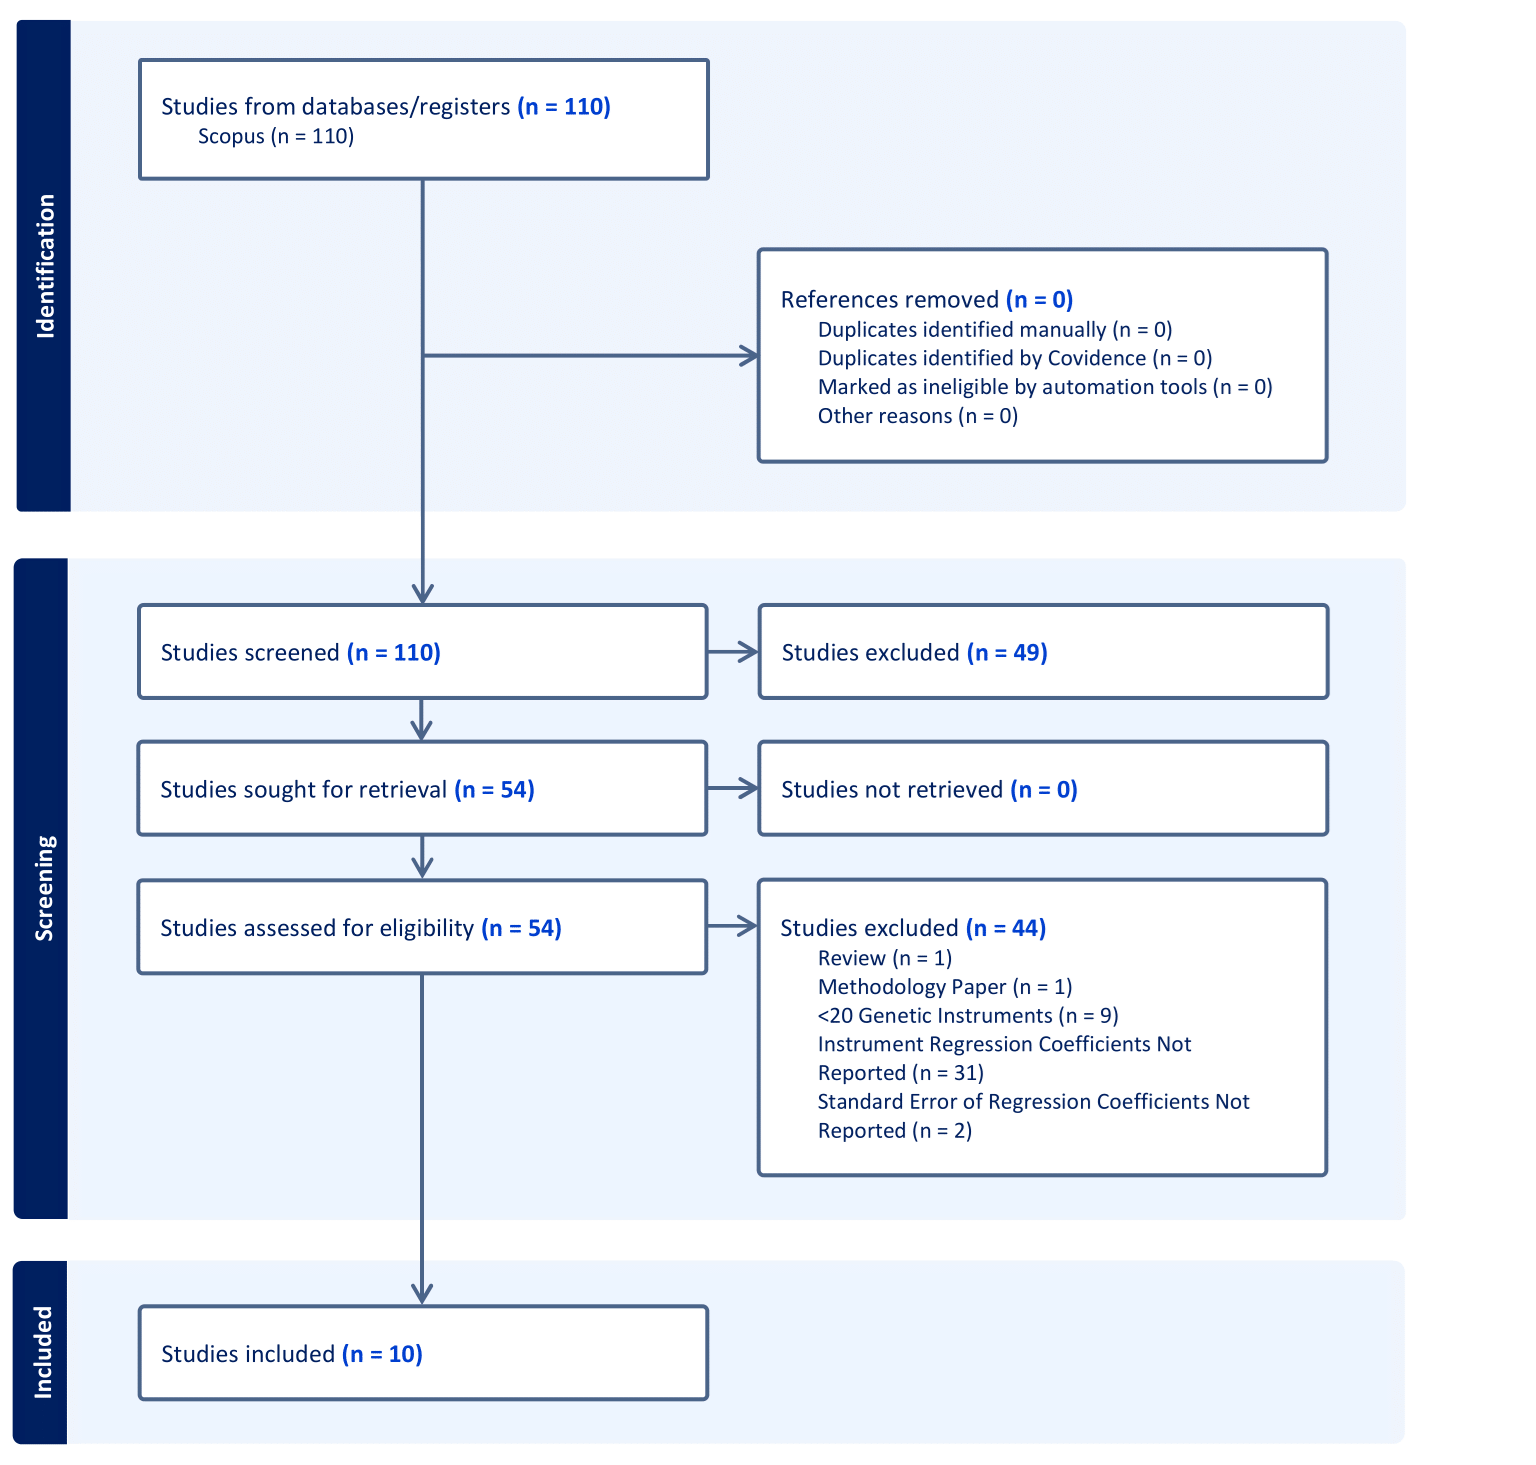
\includegraphics[width=1\linewidth,height=0.7\textheight]{Data/Citations_Search/WME_citation_search_flow_diagram_crop} \caption{Flow diagram illustrating selection of sample of ten highly-cited two-sample Mendelian randomisation articles reporting a weighted median estimate of causal effect}\label{fig:screening-flow}
\end{figure}

\begin{landscape}

\begin{Shaded}
\begin{Highlighting}[]
\FunctionTok{library}\NormalTok{(magrittr) }\CommentTok{\#bookdown forgets these packages, unclear why}
\FunctionTok{library}\NormalTok{(flextable)}
\FunctionTok{library}\NormalTok{(ftExtra)}
\FunctionTok{library}\NormalTok{(tidyverse)}

\NormalTok{citations\_search\_sample }\SpecialCharTok{\%\textgreater{}\%} 
  \FunctionTok{mutate}\NormalTok{(}
    \CommentTok{\# fill blanks}
    \CommentTok{\# Reported\_WME\_Lower\_CI = if\_else(is.na(Reported\_WME\_Lower\_CI), }
    \CommentTok{\#                                 (Reported\_WME\_Causal\_Effect {-} (1.96 * Reported\_WME\_SE)),}
    \CommentTok{\#                                 Reported\_WME\_Lower\_CI),}
    \CommentTok{\# Reported\_WME\_Upper\_CI = if\_else(is.na(Reported\_WME\_Upper\_CI),}
    \CommentTok{\#                                 (Reported\_WME\_Causal\_Effect + (1.96 * Reported\_WME\_SE)),}
    \CommentTok{\#                                 Reported\_WME\_Upper\_CI),}
    \CommentTok{\# Overlap\_Max\_Est\_Decimal = replace\_na(Overlap\_Max\_Est\_Decimal, 0),}
    \AttributeTok{p\_value =} \FunctionTok{replace\_na}\NormalTok{(p\_value, }\StringTok{"{-}"}\NormalTok{),}
    \CommentTok{\# round}
    \FunctionTok{across}\NormalTok{(}\FunctionTok{where}\NormalTok{(is.numeric), }\SpecialCharTok{\textasciitilde{}}\FunctionTok{round}\NormalTok{(., }\DecValTok{3}\NormalTok{)),}
    \CommentTok{\# combine effect estimate + CIs}
    \AttributeTok{Effect\_Estimate =} \FunctionTok{paste0}\NormalTok{(Reported\_WME\_Causal\_Effect, }\StringTok{" ("}\NormalTok{, Reported\_WME\_Lower\_CI, }\StringTok{" to "}\NormalTok{, Reported\_WME\_Upper\_CI, }\StringTok{")"}\NormalTok{),}
    \CommentTok{\# combine author/year}
    \AttributeTok{Author =} \FunctionTok{paste0}\NormalTok{(Author, }
                    \StringTok{", "}\NormalTok{,}
\NormalTok{                    Year),}
    \CommentTok{\# convert TRUE/FALSE to Yes/No}
    \AttributeTok{Causality\_Reported =} \FunctionTok{if\_else}\NormalTok{(Causality\_Reported, }\StringTok{"Yes"}\NormalTok{, }\StringTok{"No"}\NormalTok{),}
    \CommentTok{\# convert to \%}
    \AttributeTok{Participants\_Maximum\_Estimated\_Overlap =} \FunctionTok{if\_else}\NormalTok{(}\FunctionTok{is.na}\NormalTok{(Overlap\_Max\_Est\_Decimal),}
                                                     \StringTok{"0\%"}\NormalTok{,}
                                                     \FunctionTok{paste0}\NormalTok{((Overlap\_Max\_Est\_Decimal }\SpecialCharTok{*} \DecValTok{100}\NormalTok{), }\StringTok{"\%"}\NormalTok{)),}
    \CommentTok{\# change naming for flextable}
    \AttributeTok{Participants\_N\_Exposure =}\NormalTok{ Exposure\_N\_Participants,}
    \AttributeTok{Participants\_N\_Outcome =}\NormalTok{ Outcome\_N\_Participants,}
    \AttributeTok{Causal\_Effect\_Measure =}\NormalTok{ Reported\_WME\_Measure,}
    \AttributeTok{Causal\_Effect\_Estimate =}\NormalTok{ Effect\_Estimate}
    
\NormalTok{  ) }\SpecialCharTok{\%\textgreater{}\%} 
  \CommentTok{\#sort by citation count}
  \FunctionTok{arrange}\NormalTok{(Author) }\SpecialCharTok{\%\textgreater{}\%} 
  \FunctionTok{select}\NormalTok{(Author,}
         \CommentTok{\#DOI,}
\NormalTok{         Citations,}
\NormalTok{         Association,}
\NormalTok{         n\_Instruments,}
\NormalTok{         Participants\_N\_Exposure,}
\NormalTok{         Participants\_N\_Outcome,}
\NormalTok{         Participants\_Maximum\_Estimated\_Overlap,}
\NormalTok{         Causal\_Effect\_Measure,}
\NormalTok{         Causal\_Effect\_Estimate,}
\NormalTok{         Causality\_Reported,}
\NormalTok{         p\_value}
\NormalTok{         ) }\SpecialCharTok{\%\textgreater{}\%} 
  \FunctionTok{as\_flextable}\NormalTok{() }\SpecialCharTok{\%\textgreater{}\%} 
  \FunctionTok{span\_header}\NormalTok{() }\SpecialCharTok{\%\textgreater{}\%} 
  \FunctionTok{align}\NormalTok{(}\AttributeTok{part =} \StringTok{"all"}\NormalTok{, }\AttributeTok{align =} \StringTok{"center"}\NormalTok{) }\SpecialCharTok{\%\textgreater{}\%} 
  \CommentTok{\# Fix column titles}
  \DocumentationTok{\#\# N Instruments}
\NormalTok{  flextable}\SpecialCharTok{::}\FunctionTok{compose}\NormalTok{(}\AttributeTok{part =} \StringTok{"header"}\NormalTok{, }\AttributeTok{j =} \DecValTok{4}\NormalTok{, }\AttributeTok{value =} \FunctionTok{as\_paragraph}\NormalTok{(}\FunctionTok{as\_i}\NormalTok{(}\StringTok{"N"}\NormalTok{), }\StringTok{" }\SpecialCharTok{\textbackslash{}n}\StringTok{Instruments"}\NormalTok{)) }\SpecialCharTok{\%\textgreater{}\%} 
  \FunctionTok{merge\_v}\NormalTok{(}\AttributeTok{part =} \StringTok{"header"}\NormalTok{, }\AttributeTok{j =} \DecValTok{4}\NormalTok{) }\SpecialCharTok{\%\textgreater{}\%} 
  \DocumentationTok{\#\# Participants}
\NormalTok{  flextable}\SpecialCharTok{::}\FunctionTok{compose}\NormalTok{(}\AttributeTok{part =} \StringTok{"header"}\NormalTok{, }\AttributeTok{i =} \DecValTok{2}\NormalTok{, }\AttributeTok{j =} \DecValTok{5}\NormalTok{, }\AttributeTok{value =} \FunctionTok{as\_paragraph}\NormalTok{(}\FunctionTok{as\_i}\NormalTok{(}\StringTok{"N"}\NormalTok{))) }\SpecialCharTok{\%\textgreater{}\%}
  \DocumentationTok{\#\# Causality}
\NormalTok{  flextable}\SpecialCharTok{::}\FunctionTok{compose}\NormalTok{(}\AttributeTok{part =} \StringTok{"header"}\NormalTok{, }\AttributeTok{j =} \DecValTok{10}\NormalTok{, }\AttributeTok{value =} \FunctionTok{as\_paragraph}\NormalTok{(}\StringTok{"Causality Reported"}\NormalTok{)) }\SpecialCharTok{\%\textgreater{}\%} 
  \FunctionTok{merge\_v}\NormalTok{(}\AttributeTok{part =} \StringTok{"header"}\NormalTok{, }\AttributeTok{j =} \DecValTok{10}\NormalTok{) }\SpecialCharTok{\%\textgreater{}\%} 
  \DocumentationTok{\#\# p{-}value }
\NormalTok{  flextable}\SpecialCharTok{::}\FunctionTok{compose}\NormalTok{(}\AttributeTok{part =} \StringTok{"header"}\NormalTok{, }\AttributeTok{j =} \DecValTok{11}\NormalTok{, }\AttributeTok{value =} \FunctionTok{as\_paragraph}\NormalTok{(}\FunctionTok{as\_i}\NormalTok{(}\StringTok{"p"}\NormalTok{), }\StringTok{"{-}value"}\NormalTok{)) }\SpecialCharTok{\%\textgreater{}\%} 
  \FunctionTok{merge\_v}\NormalTok{(}\AttributeTok{part =} \StringTok{"header"}\NormalTok{, }\AttributeTok{j =} \DecValTok{11}\NormalTok{) }\SpecialCharTok{\%\textgreater{}\%} 
  \CommentTok{\# Add beta symbol}
\NormalTok{  flextable}\SpecialCharTok{::}\FunctionTok{compose}\NormalTok{(}\AttributeTok{part =} \StringTok{"body"}\NormalTok{, }\AttributeTok{i =} \DecValTok{8}\NormalTok{, }\AttributeTok{j =} \DecValTok{8}\NormalTok{, }\AttributeTok{value =} \FunctionTok{as\_paragraph}\NormalTok{(}\FunctionTok{as\_i}\NormalTok{(}\StringTok{"\textbackslash{}U03B2"}\NormalTok{))) }\SpecialCharTok{\%\textgreater{}\%} 
  \CommentTok{\# add lines}
  \FunctionTok{hline}\NormalTok{(}\AttributeTok{part =} \StringTok{"header"}\NormalTok{, }\AttributeTok{i =} \DecValTok{1}\NormalTok{, }\AttributeTok{j =} \FunctionTok{c}\NormalTok{(}\DecValTok{5}\SpecialCharTok{:}\DecValTok{7}\NormalTok{), }\AttributeTok{border =}\NormalTok{ officer}\SpecialCharTok{::}\FunctionTok{fp\_border}\NormalTok{(}\AttributeTok{color =} \StringTok{"black"}\NormalTok{, }\AttributeTok{width =} \DecValTok{1}\NormalTok{)) }\SpecialCharTok{\%\textgreater{}\%} 
  \FunctionTok{hline}\NormalTok{(}\AttributeTok{part =} \StringTok{"header"}\NormalTok{, }\AttributeTok{i =} \DecValTok{2}\NormalTok{, }\AttributeTok{j =} \FunctionTok{c}\NormalTok{(}\DecValTok{8}\SpecialCharTok{:}\DecValTok{9}\NormalTok{), }\AttributeTok{border =}\NormalTok{ officer}\SpecialCharTok{::}\FunctionTok{fp\_border}\NormalTok{(}\AttributeTok{color =} \StringTok{"black"}\NormalTok{, }\AttributeTok{width =} \DecValTok{1}\NormalTok{)) }\SpecialCharTok{\%\textgreater{}\%} 
  \FunctionTok{hline}\NormalTok{(}\AttributeTok{part =} \StringTok{"body"}\NormalTok{, }\AttributeTok{i =} \FunctionTok{c}\NormalTok{(}\DecValTok{1}\SpecialCharTok{:}\DecValTok{10}\NormalTok{), }\AttributeTok{j =} \FunctionTok{c}\NormalTok{(}\DecValTok{1}\SpecialCharTok{:}\DecValTok{11}\NormalTok{), }\AttributeTok{border =}\NormalTok{ officer}\SpecialCharTok{::}\FunctionTok{fp\_border}\NormalTok{(}\AttributeTok{color =} \StringTok{"black"}\NormalTok{, }\AttributeTok{width =} \FloatTok{0.2}\NormalTok{)) }\SpecialCharTok{\%\textgreater{}\%} 
  \CommentTok{\# Add footer}
  \FunctionTok{add\_footer\_lines}\NormalTok{(}\StringTok{"\textbackslash{}U03B2 and OR presented as: estimate (95\% CI).}\SpecialCharTok{\textbackslash{}n}\StringTok{\textbackslash{}U03B2: causal effect estimate, CI: Confidence Interval, OR: Odds Ratio, SE: Standard Error.}\SpecialCharTok{\textbackslash{}n}\StringTok{BMI: body mass index, CRP: C{-}reactive protein, NAFLD: non{-}alcoholic fatty liver disease, T2DM: type 2 diabetes mellitus"}\NormalTok{) }\SpecialCharTok{\%\textgreater{}\%} 
  \CommentTok{\# Formatting}
  \CommentTok{\#width(j = 2, width = 0.5,unit = "cm") \#\%\textgreater{}\% }
  \FunctionTok{fontsize}\NormalTok{(}\DecValTok{9}\NormalTok{, }\AttributeTok{i =} \FunctionTok{c}\NormalTok{(}\DecValTok{1}\SpecialCharTok{:}\DecValTok{4}\NormalTok{), }\AttributeTok{j =} \FunctionTok{c}\NormalTok{(}\DecValTok{1}\SpecialCharTok{:}\DecValTok{11}\NormalTok{), }\AttributeTok{part =} \StringTok{"header"}\NormalTok{) }\SpecialCharTok{\%\textgreater{}\%} 
  \FunctionTok{fontsize}\NormalTok{(}\DecValTok{8}\NormalTok{, }\AttributeTok{i =} \FunctionTok{c}\NormalTok{(}\DecValTok{1}\SpecialCharTok{:}\DecValTok{10}\NormalTok{), }\AttributeTok{j =} \FunctionTok{c}\NormalTok{(}\DecValTok{1}\SpecialCharTok{:}\DecValTok{11}\NormalTok{), }\AttributeTok{part =} \StringTok{"body"}\NormalTok{) }\SpecialCharTok{\%\textgreater{}\%} 
  \FunctionTok{fontsize}\NormalTok{(}\DecValTok{8}\NormalTok{, }\AttributeTok{i =} \DecValTok{1}\NormalTok{, }\AttributeTok{j =} \DecValTok{1}\NormalTok{, }\AttributeTok{part =} \StringTok{"footer"}\NormalTok{) }\SpecialCharTok{\%\textgreater{}\%} 
  \CommentTok{\#set\_table\_properties(width = 0.8, layout = "autofit") \%\textgreater{}\% }
  \FunctionTok{width}\NormalTok{(}\AttributeTok{j =} \DecValTok{3}\NormalTok{, }\AttributeTok{width =} \DecValTok{25}\NormalTok{, }\AttributeTok{unit =} \StringTok{"mm"}\NormalTok{) }\CommentTok{\#\%\textgreater{}\%}
\end{Highlighting}
\end{Shaded}

\global\setlength{\Oldarrayrulewidth}{\arrayrulewidth}

\global\setlength{\Oldtabcolsep}{\tabcolsep}

\setlength{\tabcolsep}{2pt}

\renewcommand*{\arraystretch}{1.3}



\providecommand{\ascline}[3]{\noalign{\global\arrayrulewidth #1}\arrayrulecolor[HTML]{#2}\cline{#3}}

\begin{longtable}[c]{|p{0.75in}|p{0.75in}|p{0.98in}|p{0.75in}|p{0.75in}|p{0.75in}|p{0.75in}|p{0.75in}|p{0.75in}|p{0.75in}|p{0.75in}}

\caption{Summary\ of\ ten\ highly-cited\ two-sample\ Mendelian\ randomisation\ articles\ reporting\ a\ weighted\ median\ estimate\ of\ causal\ effect}\label{tab:citation-search-sample-display}\\

\ascline{1.5pt}{666666}{1-11}

\multicolumn{1}{>{\centering}m{\dimexpr 0.75in+0\tabcolsep}}{} & \multicolumn{1}{>{\centering}m{\dimexpr 0.75in+0\tabcolsep}}{} & \multicolumn{1}{>{\centering}m{\dimexpr 0.98in+0\tabcolsep}}{} & \multicolumn{1}{>{\centering}m{\dimexpr 0.75in+0\tabcolsep}}{} & \multicolumn{3}{>{\centering}m{\dimexpr 2.25in+4\tabcolsep}}{\textcolor[HTML]{000000}{\fontsize{9}{9}\selectfont{\global\setmainfont{Arial}{Participants}}}} & \multicolumn{2}{>{\centering}m{\dimexpr 1.5in+2\tabcolsep}}{\textcolor[HTML]{000000}{\fontsize{9}{9}\selectfont{\global\setmainfont{Arial}{Causal}}}} & \multicolumn{1}{>{\centering}m{\dimexpr 0.75in+0\tabcolsep}}{} & \multicolumn{1}{>{\centering}m{\dimexpr 0.75in+0\tabcolsep}}{} \\

\ascline{1pt}{000000}{5-7}



\multicolumn{1}{>{\centering}m{\dimexpr 0.75in+0\tabcolsep}}{} & \multicolumn{1}{>{\centering}m{\dimexpr 0.75in+0\tabcolsep}}{} & \multicolumn{1}{>{\centering}m{\dimexpr 0.98in+0\tabcolsep}}{} & \multicolumn{1}{>{\centering}m{\dimexpr 0.75in+0\tabcolsep}}{} & \multicolumn{2}{>{\centering}m{\dimexpr 1.5in+2\tabcolsep}}{\textcolor[HTML]{000000}{\fontsize{9}{9}\selectfont{\global\setmainfont{Arial}{\textit{N}}}}} & \multicolumn{1}{>{\centering}m{\dimexpr 0.75in+0\tabcolsep}}{\textcolor[HTML]{000000}{\fontsize{9}{9}\selectfont{\global\setmainfont{Arial}{Maximum}}}} & \multicolumn{2}{>{\centering}m{\dimexpr 1.5in+2\tabcolsep}}{\textcolor[HTML]{000000}{\fontsize{9}{9}\selectfont{\global\setmainfont{Arial}{Effect}}}} & \multicolumn{1}{>{\centering}m{\dimexpr 0.75in+0\tabcolsep}}{} & \multicolumn{1}{>{\centering}m{\dimexpr 0.75in+0\tabcolsep}}{} \\

\ascline{1pt}{000000}{8-9}



\multicolumn{1}{>{\centering}m{\dimexpr 0.75in+0\tabcolsep}}{} & \multicolumn{1}{>{\centering}m{\dimexpr 0.75in+0\tabcolsep}}{} & \multicolumn{1}{>{\centering}m{\dimexpr 0.98in+0\tabcolsep}}{} & \multicolumn{1}{>{\centering}m{\dimexpr 0.75in+0\tabcolsep}}{} & \multicolumn{1}{>{\centering}m{\dimexpr 0.75in+0\tabcolsep}}{} & \multicolumn{1}{>{\centering}m{\dimexpr 0.75in+0\tabcolsep}}{} & \multicolumn{1}{>{\centering}m{\dimexpr 0.75in+0\tabcolsep}}{\textcolor[HTML]{000000}{\fontsize{9}{9}\selectfont{\global\setmainfont{Arial}{Estimated}}}} & \multicolumn{1}{>{\centering}m{\dimexpr 0.75in+0\tabcolsep}}{} & \multicolumn{1}{>{\centering}m{\dimexpr 0.75in+0\tabcolsep}}{} & \multicolumn{1}{>{\centering}m{\dimexpr 0.75in+0\tabcolsep}}{} & \multicolumn{1}{>{\centering}m{\dimexpr 0.75in+0\tabcolsep}}{} \\





\multicolumn{1}{>{\centering}m{\dimexpr 0.75in+0\tabcolsep}}{\multirow[c]{-4}{*}{\parbox{0.75in}{\centering \textcolor[HTML]{000000}{\fontsize{9}{9}\selectfont{\global\setmainfont{Arial}{Author}}}}}} & \multicolumn{1}{>{\centering}m{\dimexpr 0.75in+0\tabcolsep}}{\multirow[c]{-4}{*}{\parbox{0.75in}{\centering \textcolor[HTML]{000000}{\fontsize{9}{9}\selectfont{\global\setmainfont{Arial}{Citations}}}}}} & \multicolumn{1}{>{\centering}m{\dimexpr 0.98in+0\tabcolsep}}{\multirow[c]{-4}{*}{\parbox{0.98in}{\centering \textcolor[HTML]{000000}{\fontsize{9}{9}\selectfont{\global\setmainfont{Arial}{Association}}}}}} & \multicolumn{1}{>{\centering}m{\dimexpr 0.75in+0\tabcolsep}}{\multirow[c]{-4}{*}{\parbox{0.75in}{\centering \textcolor[HTML]{000000}{\fontsize{9}{9}\selectfont{\global\setmainfont{Arial}{\textit{N}}}}\textcolor[HTML]{000000}{\fontsize{9}{9}\selectfont{\global\setmainfont{Arial}{\ }}}\textcolor[HTML]{000000}{\fontsize{9}{9}\selectfont{\global\setmainfont{Arial}{\linebreak }}}\textcolor[HTML]{000000}{\fontsize{9}{9}\selectfont{\global\setmainfont{Arial}{Instruments}}}}}} & \multicolumn{1}{>{\centering}m{\dimexpr 0.75in+0\tabcolsep}}{\multirow[c]{-2}{*}{\parbox{0.75in}{\centering \textcolor[HTML]{000000}{\fontsize{9}{9}\selectfont{\global\setmainfont{Arial}{Exposure}}}}}} & \multicolumn{1}{>{\centering}m{\dimexpr 0.75in+0\tabcolsep}}{\multirow[c]{-2}{*}{\parbox{0.75in}{\centering \textcolor[HTML]{000000}{\fontsize{9}{9}\selectfont{\global\setmainfont{Arial}{Outcome}}}}}} & \multicolumn{1}{>{\centering}m{\dimexpr 0.75in+0\tabcolsep}}{\textcolor[HTML]{000000}{\fontsize{9}{9}\selectfont{\global\setmainfont{Arial}{Overlap}}}} & \multicolumn{1}{>{\centering}m{\dimexpr 0.75in+0\tabcolsep}}{\multirow[c]{-2}{*}{\parbox{0.75in}{\centering \textcolor[HTML]{000000}{\fontsize{9}{9}\selectfont{\global\setmainfont{Arial}{Measure}}}}}} & \multicolumn{1}{>{\centering}m{\dimexpr 0.75in+0\tabcolsep}}{\multirow[c]{-2}{*}{\parbox{0.75in}{\centering \textcolor[HTML]{000000}{\fontsize{9}{9}\selectfont{\global\setmainfont{Arial}{Estimate}}}}}} & \multicolumn{1}{>{\centering}m{\dimexpr 0.75in+0\tabcolsep}}{\multirow[c]{-4}{*}{\parbox{0.75in}{\centering \textcolor[HTML]{000000}{\fontsize{9}{9}\selectfont{\global\setmainfont{Arial}{Causality\ Reported}}}}}} & \multicolumn{1}{>{\centering}m{\dimexpr 0.75in+0\tabcolsep}}{\multirow[c]{-4}{*}{\parbox{0.75in}{\centering \textcolor[HTML]{000000}{\fontsize{9}{9}\selectfont{\global\setmainfont{Arial}{\textit{p}}}}\textcolor[HTML]{000000}{\fontsize{9}{9}\selectfont{\global\setmainfont{Arial}{-value}}}}}} \\

\ascline{1.5pt}{666666}{1-11}\endfirsthead \caption[]{Summary\ of\ ten\ highly-cited\ two-sample\ Mendelian\ randomisation\ articles\ reporting\ a\ weighted\ median\ estimate\ of\ causal\ effect}\label{tab:citation-search-sample-display}\\

\ascline{1.5pt}{666666}{1-11}

\multicolumn{1}{>{\centering}m{\dimexpr 0.75in+0\tabcolsep}}{} & \multicolumn{1}{>{\centering}m{\dimexpr 0.75in+0\tabcolsep}}{} & \multicolumn{1}{>{\centering}m{\dimexpr 0.98in+0\tabcolsep}}{} & \multicolumn{1}{>{\centering}m{\dimexpr 0.75in+0\tabcolsep}}{} & \multicolumn{3}{>{\centering}m{\dimexpr 2.25in+4\tabcolsep}}{\textcolor[HTML]{000000}{\fontsize{9}{9}\selectfont{\global\setmainfont{Arial}{Participants}}}} & \multicolumn{2}{>{\centering}m{\dimexpr 1.5in+2\tabcolsep}}{\textcolor[HTML]{000000}{\fontsize{9}{9}\selectfont{\global\setmainfont{Arial}{Causal}}}} & \multicolumn{1}{>{\centering}m{\dimexpr 0.75in+0\tabcolsep}}{} & \multicolumn{1}{>{\centering}m{\dimexpr 0.75in+0\tabcolsep}}{} \\

\ascline{1pt}{000000}{5-7}



\multicolumn{1}{>{\centering}m{\dimexpr 0.75in+0\tabcolsep}}{} & \multicolumn{1}{>{\centering}m{\dimexpr 0.75in+0\tabcolsep}}{} & \multicolumn{1}{>{\centering}m{\dimexpr 0.98in+0\tabcolsep}}{} & \multicolumn{1}{>{\centering}m{\dimexpr 0.75in+0\tabcolsep}}{} & \multicolumn{2}{>{\centering}m{\dimexpr 1.5in+2\tabcolsep}}{\textcolor[HTML]{000000}{\fontsize{9}{9}\selectfont{\global\setmainfont{Arial}{\textit{N}}}}} & \multicolumn{1}{>{\centering}m{\dimexpr 0.75in+0\tabcolsep}}{\textcolor[HTML]{000000}{\fontsize{9}{9}\selectfont{\global\setmainfont{Arial}{Maximum}}}} & \multicolumn{2}{>{\centering}m{\dimexpr 1.5in+2\tabcolsep}}{\textcolor[HTML]{000000}{\fontsize{9}{9}\selectfont{\global\setmainfont{Arial}{Effect}}}} & \multicolumn{1}{>{\centering}m{\dimexpr 0.75in+0\tabcolsep}}{} & \multicolumn{1}{>{\centering}m{\dimexpr 0.75in+0\tabcolsep}}{} \\

\ascline{1pt}{000000}{8-9}



\multicolumn{1}{>{\centering}m{\dimexpr 0.75in+0\tabcolsep}}{} & \multicolumn{1}{>{\centering}m{\dimexpr 0.75in+0\tabcolsep}}{} & \multicolumn{1}{>{\centering}m{\dimexpr 0.98in+0\tabcolsep}}{} & \multicolumn{1}{>{\centering}m{\dimexpr 0.75in+0\tabcolsep}}{} & \multicolumn{1}{>{\centering}m{\dimexpr 0.75in+0\tabcolsep}}{} & \multicolumn{1}{>{\centering}m{\dimexpr 0.75in+0\tabcolsep}}{} & \multicolumn{1}{>{\centering}m{\dimexpr 0.75in+0\tabcolsep}}{\textcolor[HTML]{000000}{\fontsize{9}{9}\selectfont{\global\setmainfont{Arial}{Estimated}}}} & \multicolumn{1}{>{\centering}m{\dimexpr 0.75in+0\tabcolsep}}{} & \multicolumn{1}{>{\centering}m{\dimexpr 0.75in+0\tabcolsep}}{} & \multicolumn{1}{>{\centering}m{\dimexpr 0.75in+0\tabcolsep}}{} & \multicolumn{1}{>{\centering}m{\dimexpr 0.75in+0\tabcolsep}}{} \\





\multicolumn{1}{>{\centering}m{\dimexpr 0.75in+0\tabcolsep}}{\multirow[c]{-4}{*}{\parbox{0.75in}{\centering \textcolor[HTML]{000000}{\fontsize{9}{9}\selectfont{\global\setmainfont{Arial}{Author}}}}}} & \multicolumn{1}{>{\centering}m{\dimexpr 0.75in+0\tabcolsep}}{\multirow[c]{-4}{*}{\parbox{0.75in}{\centering \textcolor[HTML]{000000}{\fontsize{9}{9}\selectfont{\global\setmainfont{Arial}{Citations}}}}}} & \multicolumn{1}{>{\centering}m{\dimexpr 0.98in+0\tabcolsep}}{\multirow[c]{-4}{*}{\parbox{0.98in}{\centering \textcolor[HTML]{000000}{\fontsize{9}{9}\selectfont{\global\setmainfont{Arial}{Association}}}}}} & \multicolumn{1}{>{\centering}m{\dimexpr 0.75in+0\tabcolsep}}{\multirow[c]{-4}{*}{\parbox{0.75in}{\centering \textcolor[HTML]{000000}{\fontsize{9}{9}\selectfont{\global\setmainfont{Arial}{\textit{N}}}}\textcolor[HTML]{000000}{\fontsize{9}{9}\selectfont{\global\setmainfont{Arial}{\ }}}\textcolor[HTML]{000000}{\fontsize{9}{9}\selectfont{\global\setmainfont{Arial}{\linebreak }}}\textcolor[HTML]{000000}{\fontsize{9}{9}\selectfont{\global\setmainfont{Arial}{Instruments}}}}}} & \multicolumn{1}{>{\centering}m{\dimexpr 0.75in+0\tabcolsep}}{\multirow[c]{-2}{*}{\parbox{0.75in}{\centering \textcolor[HTML]{000000}{\fontsize{9}{9}\selectfont{\global\setmainfont{Arial}{Exposure}}}}}} & \multicolumn{1}{>{\centering}m{\dimexpr 0.75in+0\tabcolsep}}{\multirow[c]{-2}{*}{\parbox{0.75in}{\centering \textcolor[HTML]{000000}{\fontsize{9}{9}\selectfont{\global\setmainfont{Arial}{Outcome}}}}}} & \multicolumn{1}{>{\centering}m{\dimexpr 0.75in+0\tabcolsep}}{\textcolor[HTML]{000000}{\fontsize{9}{9}\selectfont{\global\setmainfont{Arial}{Overlap}}}} & \multicolumn{1}{>{\centering}m{\dimexpr 0.75in+0\tabcolsep}}{\multirow[c]{-2}{*}{\parbox{0.75in}{\centering \textcolor[HTML]{000000}{\fontsize{9}{9}\selectfont{\global\setmainfont{Arial}{Measure}}}}}} & \multicolumn{1}{>{\centering}m{\dimexpr 0.75in+0\tabcolsep}}{\multirow[c]{-2}{*}{\parbox{0.75in}{\centering \textcolor[HTML]{000000}{\fontsize{9}{9}\selectfont{\global\setmainfont{Arial}{Estimate}}}}}} & \multicolumn{1}{>{\centering}m{\dimexpr 0.75in+0\tabcolsep}}{\multirow[c]{-4}{*}{\parbox{0.75in}{\centering \textcolor[HTML]{000000}{\fontsize{9}{9}\selectfont{\global\setmainfont{Arial}{Causality\ Reported}}}}}} & \multicolumn{1}{>{\centering}m{\dimexpr 0.75in+0\tabcolsep}}{\multirow[c]{-4}{*}{\parbox{0.75in}{\centering \textcolor[HTML]{000000}{\fontsize{9}{9}\selectfont{\global\setmainfont{Arial}{\textit{p}}}}\textcolor[HTML]{000000}{\fontsize{9}{9}\selectfont{\global\setmainfont{Arial}{-value}}}}}} \\

\ascline{1.5pt}{666666}{1-11}\endhead



\multicolumn{11}{>{\raggedright}m{\dimexpr 8.48in+20\tabcolsep}}{\textcolor[HTML]{000000}{\fontsize{8}{8}\selectfont{\global\setmainfont{Arial}{β\ and\ OR\ presented\ as:\ estimate\ (95\%\ CI).}}}\textcolor[HTML]{000000}{\fontsize{8}{8}\selectfont{\global\setmainfont{Arial}{\linebreak }}}\textcolor[HTML]{000000}{\fontsize{8}{8}\selectfont{\global\setmainfont{Arial}{β:\ causal\ effect\ estimate,\ CI:\ Confidence\ Interval,\ OR:\ Odds\ Ratio,\ SE:\ Standard\ Error.}}}\textcolor[HTML]{000000}{\fontsize{8}{8}\selectfont{\global\setmainfont{Arial}{\linebreak }}}\textcolor[HTML]{000000}{\fontsize{8}{8}\selectfont{\global\setmainfont{Arial}{BMI:\ body\ mass\ index,\ CRP:\ C-reactive\ protein,\ NAFLD:\ non-alcoholic\ fatty\ liver\ disease,\ T2DM:\ type\ 2\ diabetes\ mellitus}}}} \\

\endlastfoot



\multicolumn{1}{>{\centering}m{\dimexpr 0.75in+0\tabcolsep}}{\textcolor[HTML]{000000}{\fontsize{8}{8}\selectfont{\global\setmainfont{Arial}{Budu-Aggrey\ et\ al,\ 2019}}}} & \multicolumn{1}{>{\centering}m{\dimexpr 0.75in+0\tabcolsep}}{\textcolor[HTML]{000000}{\fontsize{8}{8}\selectfont{\global\setmainfont{Arial}{182}}}} & \multicolumn{1}{>{\centering}m{\dimexpr 0.98in+0\tabcolsep}}{\textcolor[HTML]{000000}{\fontsize{8}{8}\selectfont{\global\setmainfont{Arial}{BMI\ on\ Psoriasis}}}} & \multicolumn{1}{>{\centering}m{\dimexpr 0.75in+0\tabcolsep}}{\textcolor[HTML]{000000}{\fontsize{8}{8}\selectfont{\global\setmainfont{Arial}{97}}}} & \multicolumn{1}{>{\centering}m{\dimexpr 0.75in+0\tabcolsep}}{\textcolor[HTML]{000000}{\fontsize{8}{8}\selectfont{\global\setmainfont{Arial}{339,224}}}} & \multicolumn{1}{>{\centering}m{\dimexpr 0.75in+0\tabcolsep}}{\textcolor[HTML]{000000}{\fontsize{8}{8}\selectfont{\global\setmainfont{Arial}{12,559}}}} & \multicolumn{1}{>{\centering}m{\dimexpr 0.75in+0\tabcolsep}}{\textcolor[HTML]{000000}{\fontsize{8}{8}\selectfont{\global\setmainfont{Arial}{0\%}}}} & \multicolumn{1}{>{\centering}m{\dimexpr 0.75in+0\tabcolsep}}{\textcolor[HTML]{000000}{\fontsize{8}{8}\selectfont{\global\setmainfont{Arial}{OR}}}} & \multicolumn{1}{>{\centering}m{\dimexpr 0.75in+0\tabcolsep}}{\textcolor[HTML]{000000}{\fontsize{8}{8}\selectfont{\global\setmainfont{Arial}{1.06\ (1\ to\ 1.12)}}}} & \multicolumn{1}{>{\centering}m{\dimexpr 0.75in+0\tabcolsep}}{\textcolor[HTML]{000000}{\fontsize{8}{8}\selectfont{\global\setmainfont{Arial}{No}}}} & \multicolumn{1}{>{\centering}m{\dimexpr 0.75in+0\tabcolsep}}{\textcolor[HTML]{000000}{\fontsize{8}{8}\selectfont{\global\setmainfont{Arial}{-}}}} \\

\ascline{0.2pt}{000000}{1-11}



\multicolumn{1}{>{\centering}m{\dimexpr 0.75in+0\tabcolsep}}{\textcolor[HTML]{000000}{\fontsize{8}{8}\selectfont{\global\setmainfont{Arial}{Carreras-Torres\ et\ al,\ 2017}}}} & \multicolumn{1}{>{\centering}m{\dimexpr 0.75in+0\tabcolsep}}{\textcolor[HTML]{000000}{\fontsize{8}{8}\selectfont{\global\setmainfont{Arial}{200}}}} & \multicolumn{1}{>{\centering}m{\dimexpr 0.98in+0\tabcolsep}}{\textcolor[HTML]{000000}{\fontsize{8}{8}\selectfont{\global\setmainfont{Arial}{Height\ on\ Pancreatic\ Cancer}}}} & \multicolumn{1}{>{\centering}m{\dimexpr 0.75in+0\tabcolsep}}{\textcolor[HTML]{000000}{\fontsize{8}{8}\selectfont{\global\setmainfont{Arial}{558}}}} & \multicolumn{1}{>{\centering}m{\dimexpr 0.75in+0\tabcolsep}}{\textcolor[HTML]{000000}{\fontsize{8}{8}\selectfont{\global\setmainfont{Arial}{253,288}}}} & \multicolumn{1}{>{\centering}m{\dimexpr 0.75in+0\tabcolsep}}{\textcolor[HTML]{000000}{\fontsize{8}{8}\selectfont{\global\setmainfont{Arial}{15,002}}}} & \multicolumn{1}{>{\centering}m{\dimexpr 0.75in+0\tabcolsep}}{\textcolor[HTML]{000000}{\fontsize{8}{8}\selectfont{\global\setmainfont{Arial}{19\%}}}} & \multicolumn{1}{>{\centering}m{\dimexpr 0.75in+0\tabcolsep}}{\textcolor[HTML]{000000}{\fontsize{8}{8}\selectfont{\global\setmainfont{Arial}{OR}}}} & \multicolumn{1}{>{\centering}m{\dimexpr 0.75in+0\tabcolsep}}{\textcolor[HTML]{000000}{\fontsize{8}{8}\selectfont{\global\setmainfont{Arial}{1.14\ (1\ to\ 1.29)}}}} & \multicolumn{1}{>{\centering}m{\dimexpr 0.75in+0\tabcolsep}}{\textcolor[HTML]{000000}{\fontsize{8}{8}\selectfont{\global\setmainfont{Arial}{No}}}} & \multicolumn{1}{>{\centering}m{\dimexpr 0.75in+0\tabcolsep}}{\textcolor[HTML]{000000}{\fontsize{8}{8}\selectfont{\global\setmainfont{Arial}{0.05}}}} \\

\ascline{0.2pt}{000000}{1-11}



\multicolumn{1}{>{\centering}m{\dimexpr 0.75in+0\tabcolsep}}{\textcolor[HTML]{000000}{\fontsize{8}{8}\selectfont{\global\setmainfont{Arial}{Carter\ et\ al,\ 2019}}}} & \multicolumn{1}{>{\centering}m{\dimexpr 0.75in+0\tabcolsep}}{\textcolor[HTML]{000000}{\fontsize{8}{8}\selectfont{\global\setmainfont{Arial}{199}}}} & \multicolumn{1}{>{\centering}m{\dimexpr 0.98in+0\tabcolsep}}{\textcolor[HTML]{000000}{\fontsize{8}{8}\selectfont{\global\setmainfont{Arial}{Education\ on\ Coronary\ Disease}}}} & \multicolumn{1}{>{\centering}m{\dimexpr 0.75in+0\tabcolsep}}{\textcolor[HTML]{000000}{\fontsize{8}{8}\selectfont{\global\setmainfont{Arial}{1,267}}}} & \multicolumn{1}{>{\centering}m{\dimexpr 0.75in+0\tabcolsep}}{\textcolor[HTML]{000000}{\fontsize{8}{8}\selectfont{\global\setmainfont{Arial}{766,345}}}} & \multicolumn{1}{>{\centering}m{\dimexpr 0.75in+0\tabcolsep}}{\textcolor[HTML]{000000}{\fontsize{8}{8}\selectfont{\global\setmainfont{Arial}{184,305}}}} & \multicolumn{1}{>{\centering}m{\dimexpr 0.75in+0\tabcolsep}}{\textcolor[HTML]{000000}{\fontsize{8}{8}\selectfont{\global\setmainfont{Arial}{0\%}}}} & \multicolumn{1}{>{\centering}m{\dimexpr 0.75in+0\tabcolsep}}{\textcolor[HTML]{000000}{\fontsize{8}{8}\selectfont{\global\setmainfont{Arial}{OR}}}} & \multicolumn{1}{>{\centering}m{\dimexpr 0.75in+0\tabcolsep}}{\textcolor[HTML]{000000}{\fontsize{8}{8}\selectfont{\global\setmainfont{Arial}{0.62\ (0.57\ to\ 0.67)}}}} & \multicolumn{1}{>{\centering}m{\dimexpr 0.75in+0\tabcolsep}}{\textcolor[HTML]{000000}{\fontsize{8}{8}\selectfont{\global\setmainfont{Arial}{Yes}}}} & \multicolumn{1}{>{\centering}m{\dimexpr 0.75in+0\tabcolsep}}{\textcolor[HTML]{000000}{\fontsize{8}{8}\selectfont{\global\setmainfont{Arial}{<0.001}}}} \\

\ascline{0.2pt}{000000}{1-11}



\multicolumn{1}{>{\centering}m{\dimexpr 0.75in+0\tabcolsep}}{\textcolor[HTML]{000000}{\fontsize{8}{8}\selectfont{\global\setmainfont{Arial}{Choi\ et\ al,\ 2019}}}} & \multicolumn{1}{>{\centering}m{\dimexpr 0.75in+0\tabcolsep}}{\textcolor[HTML]{000000}{\fontsize{8}{8}\selectfont{\global\setmainfont{Arial}{492}}}} & \multicolumn{1}{>{\centering}m{\dimexpr 0.98in+0\tabcolsep}}{\textcolor[HTML]{000000}{\fontsize{8}{8}\selectfont{\global\setmainfont{Arial}{Activity\ on\ Depression}}}} & \multicolumn{1}{>{\centering}m{\dimexpr 0.75in+0\tabcolsep}}{\textcolor[HTML]{000000}{\fontsize{8}{8}\selectfont{\global\setmainfont{Arial}{24}}}} & \multicolumn{1}{>{\centering}m{\dimexpr 0.75in+0\tabcolsep}}{\textcolor[HTML]{000000}{\fontsize{8}{8}\selectfont{\global\setmainfont{Arial}{377,234}}}} & \multicolumn{1}{>{\centering}m{\dimexpr 0.75in+0\tabcolsep}}{\textcolor[HTML]{000000}{\fontsize{8}{8}\selectfont{\global\setmainfont{Arial}{143,265}}}} & \multicolumn{1}{>{\centering}m{\dimexpr 0.75in+0\tabcolsep}}{\textcolor[HTML]{000000}{\fontsize{8}{8}\selectfont{\global\setmainfont{Arial}{0\%}}}} & \multicolumn{1}{>{\centering}m{\dimexpr 0.75in+0\tabcolsep}}{\textcolor[HTML]{000000}{\fontsize{8}{8}\selectfont{\global\setmainfont{Arial}{OR}}}} & \multicolumn{1}{>{\centering}m{\dimexpr 0.75in+0\tabcolsep}}{\textcolor[HTML]{000000}{\fontsize{8}{8}\selectfont{\global\setmainfont{Arial}{1.49\ (0.94\ to\ 2.36)}}}} & \multicolumn{1}{>{\centering}m{\dimexpr 0.75in+0\tabcolsep}}{\textcolor[HTML]{000000}{\fontsize{8}{8}\selectfont{\global\setmainfont{Arial}{No}}}} & \multicolumn{1}{>{\centering}m{\dimexpr 0.75in+0\tabcolsep}}{\textcolor[HTML]{000000}{\fontsize{8}{8}\selectfont{\global\setmainfont{Arial}{0.08}}}} \\

\ascline{0.2pt}{000000}{1-11}



\multicolumn{1}{>{\centering}m{\dimexpr 0.75in+0\tabcolsep}}{\textcolor[HTML]{000000}{\fontsize{8}{8}\selectfont{\global\setmainfont{Arial}{Clift\ et\ al,\ 2022}}}} & \multicolumn{1}{>{\centering}m{\dimexpr 0.75in+0\tabcolsep}}{\textcolor[HTML]{000000}{\fontsize{8}{8}\selectfont{\global\setmainfont{Arial}{129}}}} & \multicolumn{1}{>{\centering}m{\dimexpr 0.98in+0\tabcolsep}}{\textcolor[HTML]{000000}{\fontsize{8}{8}\selectfont{\global\setmainfont{Arial}{Smoking\ Initiation\ on\ COVID-19\ Infection}}}} & \multicolumn{1}{>{\centering}m{\dimexpr 0.75in+0\tabcolsep}}{\textcolor[HTML]{000000}{\fontsize{8}{8}\selectfont{\global\setmainfont{Arial}{378}}}} & \multicolumn{1}{>{\centering}m{\dimexpr 0.75in+0\tabcolsep}}{\textcolor[HTML]{000000}{\fontsize{8}{8}\selectfont{\global\setmainfont{Arial}{1,232,091}}}} & \multicolumn{1}{>{\centering}m{\dimexpr 0.75in+0\tabcolsep}}{\textcolor[HTML]{000000}{\fontsize{8}{8}\selectfont{\global\setmainfont{Arial}{281,105}}}} & \multicolumn{1}{>{\centering}m{\dimexpr 0.75in+0\tabcolsep}}{\textcolor[HTML]{000000}{\fontsize{8}{8}\selectfont{\global\setmainfont{Arial}{36\%}}}} & \multicolumn{1}{>{\centering}m{\dimexpr 0.75in+0\tabcolsep}}{\textcolor[HTML]{000000}{\fontsize{8}{8}\selectfont{\global\setmainfont{Arial}{OR}}}} & \multicolumn{1}{>{\centering}m{\dimexpr 0.75in+0\tabcolsep}}{\textcolor[HTML]{000000}{\fontsize{8}{8}\selectfont{\global\setmainfont{Arial}{1.53\ (1.02\ to\ 2.28)}}}} & \multicolumn{1}{>{\centering}m{\dimexpr 0.75in+0\tabcolsep}}{\textcolor[HTML]{000000}{\fontsize{8}{8}\selectfont{\global\setmainfont{Arial}{Yes}}}} & \multicolumn{1}{>{\centering}m{\dimexpr 0.75in+0\tabcolsep}}{\textcolor[HTML]{000000}{\fontsize{8}{8}\selectfont{\global\setmainfont{Arial}{0.04}}}} \\

\ascline{0.2pt}{000000}{1-11}



\multicolumn{1}{>{\centering}m{\dimexpr 0.75in+0\tabcolsep}}{\textcolor[HTML]{000000}{\fontsize{8}{8}\selectfont{\global\setmainfont{Arial}{Ligthart\ et\ al,\ 2018}}}} & \multicolumn{1}{>{\centering}m{\dimexpr 0.75in+0\tabcolsep}}{\textcolor[HTML]{000000}{\fontsize{8}{8}\selectfont{\global\setmainfont{Arial}{298}}}} & \multicolumn{1}{>{\centering}m{\dimexpr 0.98in+0\tabcolsep}}{\textcolor[HTML]{000000}{\fontsize{8}{8}\selectfont{\global\setmainfont{Arial}{CRP\ on\ Schizophrenia}}}} & \multicolumn{1}{>{\centering}m{\dimexpr 0.75in+0\tabcolsep}}{\textcolor[HTML]{000000}{\fontsize{8}{8}\selectfont{\global\setmainfont{Arial}{52}}}} & \multicolumn{1}{>{\centering}m{\dimexpr 0.75in+0\tabcolsep}}{\textcolor[HTML]{000000}{\fontsize{8}{8}\selectfont{\global\setmainfont{Arial}{204,402}}}} & \multicolumn{1}{>{\centering}m{\dimexpr 0.75in+0\tabcolsep}}{\textcolor[HTML]{000000}{\fontsize{8}{8}\selectfont{\global\setmainfont{Arial}{82,315}}}} & \multicolumn{1}{>{\centering}m{\dimexpr 0.75in+0\tabcolsep}}{\textcolor[HTML]{000000}{\fontsize{8}{8}\selectfont{\global\setmainfont{Arial}{0\%}}}} & \multicolumn{1}{>{\centering}m{\dimexpr 0.75in+0\tabcolsep}}{\textcolor[HTML]{000000}{\fontsize{8}{8}\selectfont{\global\setmainfont{Arial}{OR}}}} & \multicolumn{1}{>{\centering}m{\dimexpr 0.75in+0\tabcolsep}}{\textcolor[HTML]{000000}{\fontsize{8}{8}\selectfont{\global\setmainfont{Arial}{0.89\ (0.81\ to\ 0.96)}}}} & \multicolumn{1}{>{\centering}m{\dimexpr 0.75in+0\tabcolsep}}{\textcolor[HTML]{000000}{\fontsize{8}{8}\selectfont{\global\setmainfont{Arial}{Yes}}}} & \multicolumn{1}{>{\centering}m{\dimexpr 0.75in+0\tabcolsep}}{\textcolor[HTML]{000000}{\fontsize{8}{8}\selectfont{\global\setmainfont{Arial}{0.004}}}} \\

\ascline{0.2pt}{000000}{1-11}



\multicolumn{1}{>{\centering}m{\dimexpr 0.75in+0\tabcolsep}}{\textcolor[HTML]{000000}{\fontsize{8}{8}\selectfont{\global\setmainfont{Arial}{Mokry\ et\ al,\ 2016}}}} & \multicolumn{1}{>{\centering}m{\dimexpr 0.75in+0\tabcolsep}}{\textcolor[HTML]{000000}{\fontsize{8}{8}\selectfont{\global\setmainfont{Arial}{199}}}} & \multicolumn{1}{>{\centering}m{\dimexpr 0.98in+0\tabcolsep}}{\textcolor[HTML]{000000}{\fontsize{8}{8}\selectfont{\global\setmainfont{Arial}{BMI\ on\ Multiple\ Sclerosis}}}} & \multicolumn{1}{>{\centering}m{\dimexpr 0.75in+0\tabcolsep}}{\textcolor[HTML]{000000}{\fontsize{8}{8}\selectfont{\global\setmainfont{Arial}{70}}}} & \multicolumn{1}{>{\centering}m{\dimexpr 0.75in+0\tabcolsep}}{\textcolor[HTML]{000000}{\fontsize{8}{8}\selectfont{\global\setmainfont{Arial}{322,105}}}} & \multicolumn{1}{>{\centering}m{\dimexpr 0.75in+0\tabcolsep}}{\textcolor[HTML]{000000}{\fontsize{8}{8}\selectfont{\global\setmainfont{Arial}{38,589}}}} & \multicolumn{1}{>{\centering}m{\dimexpr 0.75in+0\tabcolsep}}{\textcolor[HTML]{000000}{\fontsize{8}{8}\selectfont{\global\setmainfont{Arial}{2.5\%}}}} & \multicolumn{1}{>{\centering}m{\dimexpr 0.75in+0\tabcolsep}}{\textcolor[HTML]{000000}{\fontsize{8}{8}\selectfont{\global\setmainfont{Arial}{OR}}}} & \multicolumn{1}{>{\centering}m{\dimexpr 0.75in+0\tabcolsep}}{\textcolor[HTML]{000000}{\fontsize{8}{8}\selectfont{\global\setmainfont{Arial}{1.26\ (0.98\ to\ 1.62)}}}} & \multicolumn{1}{>{\centering}m{\dimexpr 0.75in+0\tabcolsep}}{\textcolor[HTML]{000000}{\fontsize{8}{8}\selectfont{\global\setmainfont{Arial}{No}}}} & \multicolumn{1}{>{\centering}m{\dimexpr 0.75in+0\tabcolsep}}{\textcolor[HTML]{000000}{\fontsize{8}{8}\selectfont{\global\setmainfont{Arial}{0.08}}}} \\

\ascline{0.2pt}{000000}{1-11}



\multicolumn{1}{>{\centering}m{\dimexpr 0.75in+0\tabcolsep}}{\textcolor[HTML]{000000}{\fontsize{8}{8}\selectfont{\global\setmainfont{Arial}{Pasman\ et\ al,\ 2018}}}} & \multicolumn{1}{>{\centering}m{\dimexpr 0.75in+0\tabcolsep}}{\textcolor[HTML]{000000}{\fontsize{8}{8}\selectfont{\global\setmainfont{Arial}{328}}}} & \multicolumn{1}{>{\centering}m{\dimexpr 0.98in+0\tabcolsep}}{\textcolor[HTML]{000000}{\fontsize{8}{8}\selectfont{\global\setmainfont{Arial}{Schizophrenia\ on\ Cannabis\ Use}}}} & \multicolumn{1}{>{\centering}m{\dimexpr 0.75in+0\tabcolsep}}{\textcolor[HTML]{000000}{\fontsize{8}{8}\selectfont{\global\setmainfont{Arial}{109}}}} & \multicolumn{1}{>{\centering}m{\dimexpr 0.75in+0\tabcolsep}}{\textcolor[HTML]{000000}{\fontsize{8}{8}\selectfont{\global\setmainfont{Arial}{150,064}}}} & \multicolumn{1}{>{\centering}m{\dimexpr 0.75in+0\tabcolsep}}{\textcolor[HTML]{000000}{\fontsize{8}{8}\selectfont{\global\setmainfont{Arial}{184,765}}}} & \multicolumn{1}{>{\centering}m{\dimexpr 0.75in+0\tabcolsep}}{\textcolor[HTML]{000000}{\fontsize{8}{8}\selectfont{\global\setmainfont{Arial}{0\%}}}} & \multicolumn{1}{>{\centering}m{\dimexpr 0.75in+0\tabcolsep}}{\textcolor[HTML]{000000}{\fontsize{8}{8}\selectfont{\global\setmainfont{Arial}{\textit{β}}}}} & \multicolumn{1}{>{\centering}m{\dimexpr 0.75in+0\tabcolsep}}{\textcolor[HTML]{000000}{\fontsize{8}{8}\selectfont{\global\setmainfont{Arial}{0.163\ (0.067\ to\ 0.259)}}}} & \multicolumn{1}{>{\centering}m{\dimexpr 0.75in+0\tabcolsep}}{\textcolor[HTML]{000000}{\fontsize{8}{8}\selectfont{\global\setmainfont{Arial}{Yes}}}} & \multicolumn{1}{>{\centering}m{\dimexpr 0.75in+0\tabcolsep}}{\textcolor[HTML]{000000}{\fontsize{8}{8}\selectfont{\global\setmainfont{Arial}{0.001}}}} \\

\ascline{0.2pt}{000000}{1-11}



\multicolumn{1}{>{\centering}m{\dimexpr 0.75in+0\tabcolsep}}{\textcolor[HTML]{000000}{\fontsize{8}{8}\selectfont{\global\setmainfont{Arial}{Xie\ et\ al,\ 2023}}}} & \multicolumn{1}{>{\centering}m{\dimexpr 0.75in+0\tabcolsep}}{\textcolor[HTML]{000000}{\fontsize{8}{8}\selectfont{\global\setmainfont{Arial}{138}}}} & \multicolumn{1}{>{\centering}m{\dimexpr 0.98in+0\tabcolsep}}{\textcolor[HTML]{000000}{\fontsize{8}{8}\selectfont{\global\setmainfont{Arial}{T2DM\ on\ NAFLD}}}} & \multicolumn{1}{>{\centering}m{\dimexpr 0.75in+0\tabcolsep}}{\textcolor[HTML]{000000}{\fontsize{8}{8}\selectfont{\global\setmainfont{Arial}{526}}}} & \multicolumn{1}{>{\centering}m{\dimexpr 0.75in+0\tabcolsep}}{\textcolor[HTML]{000000}{\fontsize{8}{8}\selectfont{\global\setmainfont{Arial}{441,016}}}} & \multicolumn{1}{>{\centering}m{\dimexpr 0.75in+0\tabcolsep}}{\textcolor[HTML]{000000}{\fontsize{8}{8}\selectfont{\global\setmainfont{Arial}{218,792}}}} & \multicolumn{1}{>{\centering}m{\dimexpr 0.75in+0\tabcolsep}}{\textcolor[HTML]{000000}{\fontsize{8}{8}\selectfont{\global\setmainfont{Arial}{0\%}}}} & \multicolumn{1}{>{\centering}m{\dimexpr 0.75in+0\tabcolsep}}{\textcolor[HTML]{000000}{\fontsize{8}{8}\selectfont{\global\setmainfont{Arial}{OR}}}} & \multicolumn{1}{>{\centering}m{\dimexpr 0.75in+0\tabcolsep}}{\textcolor[HTML]{000000}{\fontsize{8}{8}\selectfont{\global\setmainfont{Arial}{1.61\ (1.09\ to\ 2.38)}}}} & \multicolumn{1}{>{\centering}m{\dimexpr 0.75in+0\tabcolsep}}{\textcolor[HTML]{000000}{\fontsize{8}{8}\selectfont{\global\setmainfont{Arial}{Yes}}}} & \multicolumn{1}{>{\centering}m{\dimexpr 0.75in+0\tabcolsep}}{\textcolor[HTML]{000000}{\fontsize{8}{8}\selectfont{\global\setmainfont{Arial}{<0.001}}}} \\

\ascline{0.2pt}{000000}{1-11}



\multicolumn{1}{>{\centering}m{\dimexpr 0.75in+0\tabcolsep}}{\textcolor[HTML]{000000}{\fontsize{8}{8}\selectfont{\global\setmainfont{Arial}{Xu\ et\ al,\ 2022}}}} & \multicolumn{1}{>{\centering}m{\dimexpr 0.75in+0\tabcolsep}}{\textcolor[HTML]{000000}{\fontsize{8}{8}\selectfont{\global\setmainfont{Arial}{183}}}} & \multicolumn{1}{>{\centering}m{\dimexpr 0.98in+0\tabcolsep}}{\textcolor[HTML]{000000}{\fontsize{8}{8}\selectfont{\global\setmainfont{Arial}{Coeliac\ on\ Gut\ Bifidobacterium}}}} & \multicolumn{1}{>{\centering}m{\dimexpr 0.75in+0\tabcolsep}}{\textcolor[HTML]{000000}{\fontsize{8}{8}\selectfont{\global\setmainfont{Arial}{105}}}} & \multicolumn{1}{>{\centering}m{\dimexpr 0.75in+0\tabcolsep}}{\textcolor[HTML]{000000}{\fontsize{8}{8}\selectfont{\global\setmainfont{Arial}{15,283}}}} & \multicolumn{1}{>{\centering}m{\dimexpr 0.75in+0\tabcolsep}}{\textcolor[HTML]{000000}{\fontsize{8}{8}\selectfont{\global\setmainfont{Arial}{24,269}}}} & \multicolumn{1}{>{\centering}m{\dimexpr 0.75in+0\tabcolsep}}{\textcolor[HTML]{000000}{\fontsize{8}{8}\selectfont{\global\setmainfont{Arial}{63\%}}}} & \multicolumn{1}{>{\centering}m{\dimexpr 0.75in+0\tabcolsep}}{\textcolor[HTML]{000000}{\fontsize{8}{8}\selectfont{\global\setmainfont{Arial}{OR}}}} & \multicolumn{1}{>{\centering}m{\dimexpr 0.75in+0\tabcolsep}}{\textcolor[HTML]{000000}{\fontsize{8}{8}\selectfont{\global\setmainfont{Arial}{0.998\ (0.99\ to\ 1.005)}}}} & \multicolumn{1}{>{\centering}m{\dimexpr 0.75in+0\tabcolsep}}{\textcolor[HTML]{000000}{\fontsize{8}{8}\selectfont{\global\setmainfont{Arial}{No}}}} & \multicolumn{1}{>{\centering}m{\dimexpr 0.75in+0\tabcolsep}}{\textcolor[HTML]{000000}{\fontsize{8}{8}\selectfont{\global\setmainfont{Arial}{0.56}}}} \\

\ascline{0.2pt}{000000}{1-11}



\end{longtable}



\arrayrulecolor[HTML]{000000}

\global\setlength{\arrayrulewidth}{\Oldarrayrulewidth}

\global\setlength{\tabcolsep}{\Oldtabcolsep}

\renewcommand*{\arraystretch}{1}

\begin{Shaded}
\begin{Highlighting}[]
  \CommentTok{\#dim()}
  \CommentTok{\#autofit() \%\textgreater{}\% }
  \CommentTok{\#height\_all(height = 0.6) \%\textgreater{}\% }
  \CommentTok{\#hrule(rule = "exact", part = "all") \%\textgreater{}\% }
  \CommentTok{\#fit\_to\_width(max\_width = 9)}
  \CommentTok{\#add\_footer\_lines(".") \%\textgreater{}\%}
  \CommentTok{\# format citations}
  \CommentTok{\#flextable::compose(part = "body", i = c(1:2), j = 1, value = as\_paragraph\_md(Author))}
  \CommentTok{\#colformat\_md(part = "all", j = 1, pandoc\_args = c(\textquotesingle{}{-}{-}csl\textquotesingle{}, \textquotesingle{}harvard{-}cite{-}them{-}right.csl\textquotesingle{}))}
\end{Highlighting}
\end{Shaded}

\end{landscape}

\begin{Shaded}
\begin{Highlighting}[]
\CommentTok{\# {-}{-}{-} Citation Search {-}{-}{-} \# }

\NormalTok{data\_budu\_aggrey\_evidence\_2019 }\OtherTok{\textless{}{-}} \FunctionTok{read.csv}\NormalTok{(}\FunctionTok{here}\NormalTok{(}\StringTok{"Data"}\NormalTok{, }\StringTok{"Citations\_Datasets"}\NormalTok{, }\StringTok{"budu{-}aggrey\_evidence\_2019.csv"}\NormalTok{)) }\SpecialCharTok{\%\textgreater{}\%} \FunctionTok{as\_tibble}\NormalTok{()}
\NormalTok{data\_carreras\_torres\_role\_2017 }\OtherTok{\textless{}{-}} \FunctionTok{read.csv}\NormalTok{(}\FunctionTok{here}\NormalTok{(}\StringTok{"Data"}\NormalTok{, }\StringTok{"Citations\_Datasets"}\NormalTok{, }\StringTok{"carreras{-}torres\_role\_2017.csv"}\NormalTok{)) }\SpecialCharTok{\%\textgreater{}\%} \FunctionTok{as\_tibble}\NormalTok{()}
\NormalTok{data\_carter\_understanding\_2019 }\OtherTok{\textless{}{-}} \FunctionTok{read.csv}\NormalTok{(}\FunctionTok{here}\NormalTok{(}\StringTok{"Data"}\NormalTok{, }\StringTok{"Citations\_Datasets"}\NormalTok{, }\StringTok{"carter\_understanding\_2019.csv"}\NormalTok{)) }\SpecialCharTok{\%\textgreater{}\%} \FunctionTok{as\_tibble}\NormalTok{()}
\NormalTok{data\_choi\_assessment\_2019 }\OtherTok{\textless{}{-}} \FunctionTok{read.csv}\NormalTok{(}\FunctionTok{here}\NormalTok{(}\StringTok{"Data"}\NormalTok{, }\StringTok{"Citations\_Datasets"}\NormalTok{, }\StringTok{"choi\_assessment\_2019.csv"}\NormalTok{)) }\SpecialCharTok{\%\textgreater{}\%} \FunctionTok{as\_tibble}\NormalTok{()}
\NormalTok{data\_clift\_smoking\_2022 }\OtherTok{\textless{}{-}} \FunctionTok{read.csv}\NormalTok{(}\FunctionTok{here}\NormalTok{(}\StringTok{"Data"}\NormalTok{, }\StringTok{"Citations\_Datasets"}\NormalTok{, }\StringTok{"clift\_smoking\_2022.csv"}\NormalTok{)) }\SpecialCharTok{\%\textgreater{}\%} 
  \CommentTok{\# drop outlier \#impute outlier as mean}
  \FunctionTok{as\_tibble}\NormalTok{() }\SpecialCharTok{\%\textgreater{}\%} 
  \FunctionTok{mutate}\NormalTok{(}\FunctionTok{across}\NormalTok{(}\FunctionTok{starts\_with}\NormalTok{(}\StringTok{"Coeff\_G\_Y"}\NormalTok{), \textbackslash{}(x) }\FunctionTok{if\_else}\NormalTok{(Coeff\_G\_Y }\SpecialCharTok{==} \FunctionTok{min}\NormalTok{(Coeff\_G\_Y),}
                                                       \ConstantTok{NA\_real\_}\NormalTok{,}
                                                       \CommentTok{\#mean(x),}
\NormalTok{                                                       x)))}
  \CommentTok{\#filter(Coeff\_G\_Y!= min(Coeff\_G\_Y))}
\NormalTok{data\_ligthart\_genome\_2018 }\OtherTok{\textless{}{-}} \FunctionTok{read.csv}\NormalTok{(}\FunctionTok{here}\NormalTok{(}\StringTok{"Data"}\NormalTok{, }\StringTok{"Citations\_Datasets"}\NormalTok{, }\StringTok{"ligthart\_genome\_2018.csv"}\NormalTok{)) }\SpecialCharTok{\%\textgreater{}\%} \FunctionTok{as\_tibble}\NormalTok{()}
\NormalTok{data\_mokry\_obesity\_2016 }\OtherTok{\textless{}{-}} \FunctionTok{read.csv}\NormalTok{(}\FunctionTok{here}\NormalTok{(}\StringTok{"Data"}\NormalTok{, }\StringTok{"Citations\_Datasets"}\NormalTok{, }\StringTok{"mokry\_obesity\_2016.csv"}\NormalTok{)) }\SpecialCharTok{\%\textgreater{}\%} \FunctionTok{as\_tibble}\NormalTok{()}
\NormalTok{data\_pasman\_gwas\_2018 }\OtherTok{\textless{}{-}} \FunctionTok{read.csv}\NormalTok{(}\FunctionTok{here}\NormalTok{(}\StringTok{"Data"}\NormalTok{, }\StringTok{"Citations\_Datasets"}\NormalTok{, }\StringTok{"pasman\_gwas\_2018.csv"}\NormalTok{)) }\SpecialCharTok{\%\textgreater{}\%} \FunctionTok{as\_tibble}\NormalTok{()}
\NormalTok{data\_xie\_associations\_2023 }\OtherTok{\textless{}{-}} \FunctionTok{read.csv}\NormalTok{(}\FunctionTok{here}\NormalTok{(}\StringTok{"Data"}\NormalTok{, }\StringTok{"Citations\_Datasets"}\NormalTok{, }\StringTok{"xie\_associations\_2023.csv"}\NormalTok{)) }\SpecialCharTok{\%\textgreater{}\%} \FunctionTok{as\_tibble}\NormalTok{()}
\NormalTok{data\_xu\_causal\_2022 }\OtherTok{\textless{}{-}} \FunctionTok{read.csv}\NormalTok{(}\FunctionTok{here}\NormalTok{(}\StringTok{"Data"}\NormalTok{, }\StringTok{"Citations\_Datasets"}\NormalTok{, }\StringTok{"xu\_causal\_2022.csv"}\NormalTok{)) }\SpecialCharTok{\%\textgreater{}\%} \FunctionTok{as\_tibble}\NormalTok{()}

\CommentTok{\# Clean}
\NormalTok{citation\_datasets\_list }\OtherTok{\textless{}{-}} \FunctionTok{list}\NormalTok{(data\_budu\_aggrey\_evidence\_2019,}
\NormalTok{                               data\_carreras\_torres\_role\_2017,}
\NormalTok{                               data\_carter\_understanding\_2019,}
\NormalTok{                               data\_choi\_assessment\_2019,}
\NormalTok{                               data\_clift\_smoking\_2022,}
\NormalTok{                               data\_ligthart\_genome\_2018,}
\NormalTok{                               data\_mokry\_obesity\_2016,}
\NormalTok{                               data\_pasman\_gwas\_2018,}
\NormalTok{                               data\_xie\_associations\_2023,}
\NormalTok{                               data\_xu\_causal\_2022)}

\ControlFlowTok{for}\NormalTok{(dataset }\ControlFlowTok{in} \DecValTok{1}\SpecialCharTok{:}\FunctionTok{length}\NormalTok{(citation\_datasets\_list))\{}
  
\NormalTok{  citation\_datasets\_list[[dataset]] }\OtherTok{\textless{}{-}}\NormalTok{ citation\_datasets\_list[[dataset]] }\SpecialCharTok{\%\textgreater{}\%} 
    \FunctionTok{tibble}\NormalTok{() }\SpecialCharTok{\%\textgreater{}\%} 
    \FunctionTok{mutate}\NormalTok{(}
      \CommentTok{\# replace all unicode dash variations with minus {-} to stop conversion to char}
      \CommentTok{\# https://stackoverflow.com/questions/48923599/searching{-}for{-}all{-}variations{-}of{-}hyphens{-}and{-}dashes{-}in{-}regex}
      \FunctionTok{across}\NormalTok{(}\FunctionTok{starts\_with}\NormalTok{(}\StringTok{"Coeff\_"}\NormalTok{), }
             \SpecialCharTok{\textasciitilde{}}\FunctionTok{str\_replace\_all}\NormalTok{(.,}
                              \AttributeTok{pattern =} \StringTok{"[\textbackslash{}u002D\textbackslash{}u058A\textbackslash{}u05BE\textbackslash{}u1400\textbackslash{}u1806\textbackslash{}u2010{-}\textbackslash{}u2015\textbackslash{}u2E17\textbackslash{}u2E1A\textbackslash{}u2E3A\textbackslash{}u2E3B\textbackslash{}u2E40\textbackslash{}u301C\textbackslash{}u3030\textbackslash{}u30A0\textbackslash{}uFE31\textbackslash{}uFE32\textbackslash{}uFE58\textbackslash{}uFE63\textbackslash{}uFF0D]"}\NormalTok{, }
                              \CommentTok{\# https://www.kaggle.com/discussions/questions{-}and{-}answers/54715}
                              \AttributeTok{replacement =} \StringTok{"\textbackslash{}U002D"}\NormalTok{)),}
      \CommentTok{\# encode missing as NA }
      \FunctionTok{across}\NormalTok{(}\FunctionTok{starts\_with}\NormalTok{(}\StringTok{"Coeff\_"}\NormalTok{), }\SpecialCharTok{\textasciitilde{}}\FunctionTok{str\_replace\_all}\NormalTok{(., }\AttributeTok{pattern =} \StringTok{"[Aa:Zz]"}\NormalTok{, }\AttributeTok{replacement =} \ConstantTok{NA\_character\_}\NormalTok{)),}
      \FunctionTok{across}\NormalTok{(}\FunctionTok{starts\_with}\NormalTok{(}\StringTok{"Coeff\_"}\NormalTok{), }\SpecialCharTok{\textasciitilde{}}\FunctionTok{as.double}\NormalTok{(.)),}
      \CommentTok{\#across(where(is.numeric), \textasciitilde{}replace\_na(., mean(., na.rm = TRUE)) ), \#imputes missing as mean}
      \CommentTok{\# replace zeros for MR{-}Hevo}
      \FunctionTok{across}\NormalTok{(}\FunctionTok{starts\_with}\NormalTok{(}\StringTok{"Coeff\_"}\NormalTok{), }\SpecialCharTok{\textasciitilde{}}\FunctionTok{replace}\NormalTok{(., . }\SpecialCharTok{==} \DecValTok{0}\NormalTok{, }\DecValTok{10}\SpecialCharTok{\^{}{-}}\DecValTok{100}\NormalTok{)), }
      \CommentTok{\# remove square brackets from ref tags}
      \FunctionTok{across}\NormalTok{(Study\_Ref, }\SpecialCharTok{\textasciitilde{}}\FunctionTok{str\_replace\_all}\NormalTok{(., }\StringTok{"}\SpecialCharTok{\textbackslash{}\textbackslash{}}\StringTok{[|}\SpecialCharTok{\textbackslash{}\textbackslash{}}\StringTok{]"}\NormalTok{, }\StringTok{""}\NormalTok{))}
\NormalTok{    )}
    
\NormalTok{\}}


\CommentTok{\# Combine}
\NormalTok{Citations\_Instrument\_Data }\OtherTok{\textless{}{-}} \FunctionTok{bind\_rows}\NormalTok{(citation\_datasets\_list)}

\CommentTok{\# Write to .csv}
\FunctionTok{write.csv}\NormalTok{(Citations\_Instrument\_Data, }\FunctionTok{here}\NormalTok{(}\StringTok{"Data"}\NormalTok{, }\StringTok{"Citations\_Datasets"}\NormalTok{, }\StringTok{"Citations\_Instrument\_Data.csv"}\NormalTok{),}\AttributeTok{append =} \ConstantTok{FALSE}\NormalTok{)}

\CommentTok{\# \# Check}
\CommentTok{\# Citations\_Instrument\_Data \%\textgreater{}\%}
\CommentTok{\#   head()}
\CommentTok{\#   }
\CommentTok{\# Citations\_Instrument\_Data \%\textgreater{}\% }
\CommentTok{\#   group\_by(Author) \%\textgreater{}\% }
\CommentTok{\#   summarise(across(everything(), \textbackslash{}(x) sum(is.na(x)))) \%\textgreater{}\% }
\CommentTok{\#   print()}
\CommentTok{\# Citations\_Instrument\_Data \%\textgreater{}\%}
\CommentTok{\#   group\_by(Author) \%\textgreater{}\% }
\CommentTok{\#   summarise(}
\CommentTok{\#     Mean\_G\_X = mean(Coeff\_G\_X),}
\CommentTok{\#     Min\_G\_X = min(Coeff\_G\_X),}
\CommentTok{\#     Max\_G\_X = max(Coeff\_G\_X),}
\CommentTok{\#     Mean\_G\_X\_SE = mean(Coeff\_G\_X\_SE),}
\CommentTok{\#     Min\_G\_X\_SE = min(Coeff\_G\_X\_SE),}
\CommentTok{\#     Max\_G\_X\_SE = max(Coeff\_G\_X\_SE),}
\CommentTok{\#     Mean\_G\_Y = mean(Coeff\_G\_Y),}
\CommentTok{\#     Min\_G\_Y = min(Coeff\_G\_Y),}
\CommentTok{\#     Max\_G\_Y = max(Coeff\_G\_Y),}
\CommentTok{\#     Mean\_G\_Y\_SE = mean(Coeff\_G\_Y\_SE),}
\CommentTok{\#     Min\_G\_Y\_SE = min(Coeff\_G\_Y\_SE),}
\CommentTok{\#     Max\_G\_Y\_SE = max(Coeff\_G\_Y\_SE)) \%\textgreater{}\% }
\CommentTok{\#   mutate(across(where(is.numeric), \textbackslash{}(x) round(x, 2))) \%\textgreater{}\%}
\CommentTok{\#   print()}
\CommentTok{\# }
\CommentTok{\# citation\_datasets\_list[[9]] \%\textgreater{}\% }
\CommentTok{\#   filter(if\_any(everything(), is.na)) \%\textgreater{}\% }
\CommentTok{\#   print()}

\CommentTok{\#Citations\_Instrument\_Data}
\end{Highlighting}
\end{Shaded}

\subsubsection{Re-Analysis Results}\label{re-analysis-results}

\begin{Shaded}
\begin{Highlighting}[]
\NormalTok{citations\_reanalysis\_summ\_tib }\OtherTok{\textless{}{-}} \FunctionTok{readRDS}\NormalTok{(}\FunctionTok{here}\NormalTok{(}\StringTok{"Data"}\NormalTok{, }\StringTok{"Summary\_Tables"}\NormalTok{, }\StringTok{"citations\_reanalysis\_summ\_tib.rds"}\NormalTok{)) }\SpecialCharTok{\%\textgreater{}\%} 
  \FunctionTok{tibble}\NormalTok{() }\SpecialCharTok{\%\textgreater{}\%} 
  \FunctionTok{mutate}\NormalTok{(}\FunctionTok{across}\NormalTok{(Study\_Ref, }\SpecialCharTok{\textasciitilde{}}\FunctionTok{str\_replace\_all}\NormalTok{(., }\StringTok{"}\SpecialCharTok{\textbackslash{}\textbackslash{}}\StringTok{[|}\SpecialCharTok{\textbackslash{}\textbackslash{}}\StringTok{]"}\NormalTok{, }\StringTok{""}\NormalTok{))) }\CommentTok{\#\%\textgreater{}\% }
  \CommentTok{\#rename(Hevo\_WME\_Causal\_Discordant = Discordant)}

\CommentTok{\# Join both citation tables for comparisons}
\NormalTok{citations\_combined\_summ\_tib }\OtherTok{\textless{}{-}} \FunctionTok{left\_join}\NormalTok{(}\AttributeTok{x =}\NormalTok{ citations\_reanalysis\_summ\_tib, }\AttributeTok{y =}\NormalTok{citations\_search\_sample)}

\NormalTok{citations\_combined\_summ\_tib }\OtherTok{\textless{}{-}}\NormalTok{ citations\_combined\_summ\_tib }\SpecialCharTok{\%\textgreater{}\%} 
  \FunctionTok{mutate}\NormalTok{(}
    \CommentTok{\#{-}{-}{-} Re{-}analysed WME values vs original reports {-}{-}{-}\#}
    \DocumentationTok{\#\# Estimates}
    \AttributeTok{Diff\_WME\_Causal\_Est =} \FunctionTok{if\_else}\NormalTok{(Reported\_WME\_Measure }\SpecialCharTok{==} \StringTok{"OR"}\NormalTok{,}
\NormalTok{                                  Reported\_WME\_Causal\_Effect }\SpecialCharTok{{-}}\NormalTok{ WME\_OR,}
\NormalTok{                                  Reported\_WME\_Causal\_Effect }\SpecialCharTok{{-}}\NormalTok{ WME\_est),}
    \AttributeTok{Diff\_WME\_Est\_Over\_Point1 =}\NormalTok{ (}\FunctionTok{abs}\NormalTok{(Diff\_WME\_Causal\_Est) }\SpecialCharTok{\textgreater{}} \FloatTok{0.1}\NormalTok{),}
    \AttributeTok{Auth\_Cite\_Diff\_WME\_Est\_Over\_Point1 =} \FunctionTok{if\_else}\NormalTok{(Diff\_WME\_Est\_Over\_Point1,}
                                             \FunctionTok{paste0}\NormalTok{(Study\_Author, }\StringTok{"["}\NormalTok{, Study\_Ref, }\StringTok{"]"}\NormalTok{),}
                                             \ConstantTok{NA}\NormalTok{),}
    \DocumentationTok{\#\# CIs}
    \AttributeTok{Diff\_WME\_Causal\_Low =} \FunctionTok{if\_else}\NormalTok{(Reported\_WME\_Measure }\SpecialCharTok{==} \StringTok{"OR"}\NormalTok{,}
\NormalTok{                                  Reported\_WME\_Lower\_CI }\SpecialCharTok{{-}}\NormalTok{ WME\_OR\_lower\_CI,}
\NormalTok{                                  Reported\_WME\_Lower\_CI }\SpecialCharTok{{-}}\NormalTok{ WME\_est\_lower\_CI),}
    \AttributeTok{Diff\_WME\_Causal\_Upp =} \FunctionTok{if\_else}\NormalTok{(Reported\_WME\_Measure }\SpecialCharTok{==} \StringTok{"OR"}\NormalTok{,}
\NormalTok{                                  Reported\_WME\_Upper\_CI }\SpecialCharTok{{-}}\NormalTok{ WME\_OR\_upper\_CI,}
\NormalTok{                                  Reported\_WME\_Upper\_CI }\SpecialCharTok{{-}}\NormalTok{ WME\_est\_upper\_CI),}
    \AttributeTok{Diff\_WME\_CIs\_Over\_Point1 =}\NormalTok{ (}\FunctionTok{abs}\NormalTok{(Diff\_WME\_Causal\_Low }\SpecialCharTok{\textgreater{}} \FloatTok{0.1}\NormalTok{) }\SpecialCharTok{|} \FunctionTok{abs}\NormalTok{(Diff\_WME\_Causal\_Upp) }\SpecialCharTok{\textgreater{}}\FloatTok{0.1}\NormalTok{),}
    \AttributeTok{Auth\_Cite\_Diff\_WME\_CIs\_Over\_Point1 =} \FunctionTok{if\_else}\NormalTok{(Diff\_WME\_CIs\_Over\_Point1,}
                                             \FunctionTok{paste0}\NormalTok{(Study\_Author, }\StringTok{"["}\NormalTok{, Study\_Ref, }\StringTok{"]"}\NormalTok{),}
                                             \ConstantTok{NA}\NormalTok{),}
    \DocumentationTok{\#\# SE}
    \AttributeTok{Diff\_WME\_SE =} \FunctionTok{if\_else}\NormalTok{(}\FunctionTok{is.na}\NormalTok{(Reported\_WME\_SE),}
\NormalTok{                          (Reported\_WME\_Upper\_CI }\SpecialCharTok{{-}}\NormalTok{ Reported\_WME\_Causal\_Effect) }\SpecialCharTok{/} \FloatTok{1.96}\NormalTok{,}
\NormalTok{                          Reported\_WME\_SE),}
    \AttributeTok{Diff\_WME\_SE\_Over\_Point1 =}\NormalTok{ (}\FunctionTok{abs}\NormalTok{(Diff\_WME\_SE) }\SpecialCharTok{\textgreater{}} \FloatTok{0.1}\NormalTok{),}
    \AttributeTok{Auth\_Cite\_Diff\_WME\_SE\_Over\_Point1 =} \FunctionTok{if\_else}\NormalTok{(Diff\_WME\_SE\_Over\_Point1,}
                                                \FunctionTok{paste0}\NormalTok{(Study\_Author, }\StringTok{"["}\NormalTok{, Study\_Ref, }\StringTok{"]"}\NormalTok{),}
                                                \ConstantTok{NA}\NormalTok{),}
    \FunctionTok{across}\NormalTok{(}\FunctionTok{where}\NormalTok{(is.numeric), \textbackslash{}(x) }\FunctionTok{round}\NormalTok{(x, }\DecValTok{2}\NormalTok{)),}
    \DocumentationTok{\#\# Comparables}
    \AttributeTok{Comp\_WME\_Est\_CI =}\NormalTok{ (}\SpecialCharTok{!}\NormalTok{Diff\_WME\_Est\_Over\_Point1 }\SpecialCharTok{\&} \SpecialCharTok{!}\NormalTok{Diff\_WME\_CIs\_Over\_Point1),}
    \AttributeTok{Auth\_Cite\_Comp\_WME\_Est\_CI =} \FunctionTok{if\_else}\NormalTok{(Comp\_WME\_Est\_CI,}
                                        \FunctionTok{paste0}\NormalTok{(Study\_Author, }\StringTok{"["}\NormalTok{, Study\_Ref, }\StringTok{"]"}\NormalTok{),}
                                        \ConstantTok{NA}\NormalTok{),}
    \DocumentationTok{\#\# Causal Reports}
    \AttributeTok{Diff\_WME\_Causal\_Report =}\NormalTok{ (Causality\_Reported }\SpecialCharTok{!=}\NormalTok{ WME\_est\_causal\_detected),}
    \AttributeTok{Diff\_WME\_Causal\_To\_No\_Causal =}\NormalTok{ (Causality\_Reported }\SpecialCharTok{==} \ConstantTok{TRUE} \SpecialCharTok{\&}\NormalTok{ WME\_est\_causal\_detected }\SpecialCharTok{==} \ConstantTok{FALSE}\NormalTok{),}
    \AttributeTok{Auth\_Cite\_WME\_Causal\_To\_No\_Causal =} \FunctionTok{if\_else}\NormalTok{(Diff\_WME\_Causal\_To\_No\_Causal,}
                                                \FunctionTok{paste0}\NormalTok{(Study\_Author, }\StringTok{"["}\NormalTok{, Study\_Ref, }\StringTok{"]"}\NormalTok{),}
                                                \ConstantTok{NA}\NormalTok{),}
    \AttributeTok{Diff\_WME\_No\_Causal\_To\_Causal =}\NormalTok{ (Causality\_Reported }\SpecialCharTok{==} \ConstantTok{FALSE} \SpecialCharTok{\&}\NormalTok{ WME\_est\_causal\_detected }\SpecialCharTok{==} \ConstantTok{TRUE}\NormalTok{),}
    \AttributeTok{Auth\_Cite\_WME\_No\_Causal\_To\_Causal =} \FunctionTok{if\_else}\NormalTok{(Diff\_WME\_No\_Causal\_To\_Causal,}
                                                \FunctionTok{paste0}\NormalTok{(Study\_Author, }\StringTok{"["}\NormalTok{, Study\_Ref, }\StringTok{"]"}\NormalTok{),}
                                                \ConstantTok{NA}\NormalTok{),}
    \CommentTok{\#{-}{-}{-} MR{-}Hevo vs re{-}analysed WME {-}{-}{-}\# }
    \DocumentationTok{\#\# Estimates}
    \AttributeTok{Diff\_Hevo\_WME\_Causal\_Est =} \FunctionTok{if\_else}\NormalTok{(Reported\_WME\_Measure }\SpecialCharTok{==} \StringTok{"OR"}\NormalTok{,}
\NormalTok{                                       Hevo\_OR }\SpecialCharTok{{-}}\NormalTok{ WME\_OR,}
\NormalTok{                                       Hevo\_est }\SpecialCharTok{{-}}\NormalTok{ WME\_est),}
    \AttributeTok{Diff\_Hevo\_WME\_Est\_Over\_Point1 =}\NormalTok{ (}\FunctionTok{abs}\NormalTok{(Diff\_Hevo\_WME\_Causal\_Est) }\SpecialCharTok{\textgreater{}} \FloatTok{0.1}\NormalTok{),}
    \AttributeTok{Auth\_Cite\_Diff\_Hevo\_WME\_Est\_Over\_Point1 =} \FunctionTok{if\_else}\NormalTok{(Diff\_Hevo\_WME\_Est\_Over\_Point1,}
                                                      \FunctionTok{paste0}\NormalTok{(Study\_Author, }\StringTok{"["}\NormalTok{, Study\_Ref, }\StringTok{"]"}\NormalTok{),}
                                                      \ConstantTok{NA}\NormalTok{),}
    \DocumentationTok{\#\# CIs}
    \AttributeTok{Diff\_Hevo\_WME\_Causal\_Low =} \FunctionTok{if\_else}\NormalTok{(Reported\_WME\_Measure }\SpecialCharTok{==} \StringTok{"OR"}\NormalTok{,}
\NormalTok{                                       Hevo\_OR\_lower\_CI }\SpecialCharTok{{-}}\NormalTok{ WME\_OR\_lower\_CI,}
\NormalTok{                                       Hevo\_est\_lower\_CI }\SpecialCharTok{{-}}\NormalTok{ WME\_est\_lower\_CI),}
    \AttributeTok{Diff\_Hevo\_WME\_Causal\_Upp =} \FunctionTok{if\_else}\NormalTok{(Reported\_WME\_Measure }\SpecialCharTok{==} \StringTok{"OR"}\NormalTok{,}
\NormalTok{                                       Hevo\_OR\_upper\_CI }\SpecialCharTok{{-}}\NormalTok{ WME\_OR\_upper\_CI,}
\NormalTok{                                       Hevo\_est\_upper\_CI }\SpecialCharTok{{-}}\NormalTok{ WME\_est\_upper\_CI),}
    \AttributeTok{Diff\_Hevo\_WME\_CIs\_Over\_Point1 =}\NormalTok{ (}\FunctionTok{abs}\NormalTok{(Diff\_Hevo\_WME\_Causal\_Low }\SpecialCharTok{\textgreater{}} \FloatTok{0.1}\NormalTok{) }\SpecialCharTok{|} \FunctionTok{abs}\NormalTok{(Diff\_Hevo\_WME\_Causal\_Upp) }\SpecialCharTok{\textgreater{}}\FloatTok{0.1}\NormalTok{),}
    \AttributeTok{Auth\_Cite\_Diff\_Hevo\_WME\_CIs\_Over\_Point1 =} \FunctionTok{if\_else}\NormalTok{(Diff\_Hevo\_WME\_CIs\_Over\_Point1,}
                                                      \FunctionTok{paste0}\NormalTok{(Study\_Author, }\StringTok{"["}\NormalTok{, Study\_Ref, }\StringTok{"]"}\NormalTok{),}
                                                      \ConstantTok{NA}\NormalTok{),}
    \DocumentationTok{\#\# SE}
    \AttributeTok{Diff\_Hevo\_WME\_SE =}\NormalTok{ Hevo\_se }\SpecialCharTok{{-}}\NormalTok{ WME\_se,}
    \AttributeTok{Diff\_Hevo\_WME\_SE\_Over\_Point1 =}\NormalTok{ (}\FunctionTok{abs}\NormalTok{(Diff\_Hevo\_WME\_SE) }\SpecialCharTok{\textgreater{}} \FloatTok{0.1}\NormalTok{),}
    \AttributeTok{Auth\_Cite\_Diff\_Hevo\_WME\_SE\_Over\_Point1 =} \FunctionTok{if\_else}\NormalTok{(Diff\_Hevo\_WME\_SE\_Over\_Point1,}
                                                     \FunctionTok{paste0}\NormalTok{(Study\_Author, }\StringTok{"["}\NormalTok{, Study\_Ref, }\StringTok{"]"}\NormalTok{),}
                                                     \ConstantTok{NA}\NormalTok{),}
    \FunctionTok{across}\NormalTok{(}\FunctionTok{where}\NormalTok{(is.numeric), \textbackslash{}(x) }\FunctionTok{round}\NormalTok{(x, }\DecValTok{2}\NormalTok{)),}
    \DocumentationTok{\#\# Comparables}
    \AttributeTok{Comp\_Hevo\_WME\_Est\_CI =}\NormalTok{ (}\SpecialCharTok{!}\NormalTok{Diff\_Hevo\_WME\_Est\_Over\_Point1 }\SpecialCharTok{\&} \SpecialCharTok{!}\NormalTok{Diff\_Hevo\_WME\_CIs\_Over\_Point1),}
    \AttributeTok{Auth\_Cite\_Comp\_Hevo\_WME\_Est\_CI =} \FunctionTok{if\_else}\NormalTok{(Comp\_Hevo\_WME\_Est\_CI,}
                                             \FunctionTok{paste0}\NormalTok{(Study\_Author, }\StringTok{"["}\NormalTok{, Study\_Ref, }\StringTok{"]"}\NormalTok{),}
                                             \ConstantTok{NA}\NormalTok{),}
    \DocumentationTok{\#\# Causal Reports}
    \AttributeTok{Diff\_Hevo\_WME\_Causal\_Report =}\NormalTok{ (Hevo\_est\_causal\_detected }\SpecialCharTok{!=}\NormalTok{ WME\_est\_causal\_detected),}
    \AttributeTok{Diff\_Hevo\_Causal\_WME\_No\_Causal =}\NormalTok{ (Hevo\_est\_causal\_detected }\SpecialCharTok{==} \ConstantTok{TRUE} \SpecialCharTok{\&}\NormalTok{ WME\_est\_causal\_detected }\SpecialCharTok{==} \ConstantTok{FALSE}\NormalTok{),}
    \AttributeTok{Auth\_Cite\_Hevo\_Causal\_WME\_No\_Causal =} \FunctionTok{if\_else}\NormalTok{(Diff\_Hevo\_Causal\_WME\_No\_Causal,}
                                                  \FunctionTok{paste0}\NormalTok{(Study\_Author, }\StringTok{"["}\NormalTok{, Study\_Ref, }\StringTok{"]"}\NormalTok{),}
                                                  \ConstantTok{NA}\NormalTok{),}
    \AttributeTok{Diff\_Hevo\_No\_Causal\_WME\_Causal =}\NormalTok{ (Hevo\_est\_causal\_detected }\SpecialCharTok{==} \ConstantTok{FALSE} \SpecialCharTok{\&}\NormalTok{ WME\_est\_causal\_detected }\SpecialCharTok{==} \ConstantTok{TRUE}\NormalTok{),}
    \AttributeTok{Auth\_Cite\_Hevo\_No\_Causal\_WME\_Causal =} \FunctionTok{if\_else}\NormalTok{(Diff\_Hevo\_No\_Causal\_WME\_Causal,}
                                                  \FunctionTok{paste0}\NormalTok{(Study\_Author, }\StringTok{"["}\NormalTok{, Study\_Ref, }\StringTok{"]"}\NormalTok{),}
                                                  \ConstantTok{NA}\NormalTok{)}
\NormalTok{  )}

\DocumentationTok{\#\# Mean diffs}

\NormalTok{WME\_diff\_mean\_OR }\OtherTok{\textless{}{-}}\NormalTok{ citations\_combined\_summ\_tib }\SpecialCharTok{\%\textgreater{}\%} 
  \FunctionTok{filter}\NormalTok{(Reported\_WME\_Measure }\SpecialCharTok{==} \StringTok{"OR"}\NormalTok{) }\SpecialCharTok{\%\textgreater{}\%}
  \FunctionTok{summarise}\NormalTok{(}
    \AttributeTok{est\_diff =} \FunctionTok{mean}\NormalTok{(Diff\_WME\_Causal\_Est),}
    \AttributeTok{se\_diff =} \FunctionTok{mean}\NormalTok{(Diff\_WME\_SE),}
    \AttributeTok{lower\_diff =} \FunctionTok{mean}\NormalTok{(Diff\_WME\_Causal\_Low),}
    \AttributeTok{upper\_diff =} \FunctionTok{mean}\NormalTok{(Diff\_WME\_Causal\_Upp),}
    \AttributeTok{N =} \FunctionTok{nrow}\NormalTok{(.)}
\NormalTok{  ) }\SpecialCharTok{\%\textgreater{}\%} 
  \FunctionTok{mutate}\NormalTok{(}\FunctionTok{across}\NormalTok{(}\FunctionTok{where}\NormalTok{(is.numeric), \textbackslash{}(x) }\FunctionTok{round}\NormalTok{(x, }\DecValTok{2}\NormalTok{)))}







\CommentTok{\# citations\_reanalysis\_summ\_tib}
\CommentTok{\# citations\_search\_sample}
\CommentTok{\# citations\_combined\_summ\_tib}
\end{Highlighting}
\end{Shaded}

\begin{Shaded}
\begin{Highlighting}[]
\CommentTok{\# Comparing re{-}analysis WME values and original reports}

\DocumentationTok{\#\# Different Estimates}
\NormalTok{diff\_WME\_est\_over\_point1\_N }\OtherTok{\textless{}{-}} \FunctionTok{sum}\NormalTok{(citations\_combined\_summ\_tib}\SpecialCharTok{$}\NormalTok{Diff\_WME\_Est\_Over\_Point1)}
\NormalTok{diff\_WME\_est\_over\_point1\_cites }\OtherTok{\textless{}{-}}\NormalTok{ citations\_combined\_summ\_tib }\SpecialCharTok{\%\textgreater{}\%} 
  \FunctionTok{filter}\NormalTok{(}\SpecialCharTok{!}\FunctionTok{is.na}\NormalTok{(Auth\_Cite\_Diff\_WME\_Est\_Over\_Point1)) }\SpecialCharTok{\%\textgreater{}\%} 
  \FunctionTok{pull}\NormalTok{(Auth\_Cite\_Diff\_WME\_Est\_Over\_Point1) }\SpecialCharTok{\%\textgreater{}\%} 
  \FunctionTok{paste}\NormalTok{(}\AttributeTok{collapse =} \StringTok{", "}\NormalTok{)}

\DocumentationTok{\#\# Different SEs}
\NormalTok{diff\_WME\_se\_over\_point1\_N }\OtherTok{\textless{}{-}} \FunctionTok{sum}\NormalTok{(citations\_combined\_summ\_tib}\SpecialCharTok{$}\NormalTok{Diff\_WME\_SE\_Over\_Point1)}
\NormalTok{diff\_WME\_se\_over\_point1\_cites }\OtherTok{\textless{}{-}}\NormalTok{ citations\_combined\_summ\_tib }\SpecialCharTok{\%\textgreater{}\%} 
  \FunctionTok{filter}\NormalTok{(}\SpecialCharTok{!}\FunctionTok{is.na}\NormalTok{(Auth\_Cite\_Diff\_WME\_SE\_Over\_Point1)) }\SpecialCharTok{\%\textgreater{}\%} 
  \FunctionTok{pull}\NormalTok{(Auth\_Cite\_Diff\_WME\_SE\_Over\_Point1) }\SpecialCharTok{\%\textgreater{}\%} 
  \FunctionTok{paste}\NormalTok{(}\AttributeTok{collapse =} \StringTok{", "}\NormalTok{)}

\DocumentationTok{\#\# Different CIs}
\NormalTok{diff\_WME\_CIs\_over\_point1\_N }\OtherTok{\textless{}{-}} \FunctionTok{sum}\NormalTok{(citations\_combined\_summ\_tib}\SpecialCharTok{$}\NormalTok{Diff\_WME\_CIs\_Over\_Point1)}
\NormalTok{diff\_WME\_CIs\_over\_point1\_cites }\OtherTok{\textless{}{-}}\NormalTok{ citations\_combined\_summ\_tib }\SpecialCharTok{\%\textgreater{}\%} 
  \FunctionTok{filter}\NormalTok{(}\SpecialCharTok{!}\FunctionTok{is.na}\NormalTok{(Auth\_Cite\_Diff\_WME\_CIs\_Over\_Point1)) }\SpecialCharTok{\%\textgreater{}\%} 
  \FunctionTok{pull}\NormalTok{(Auth\_Cite\_Diff\_WME\_CIs\_Over\_Point1) }\SpecialCharTok{\%\textgreater{}\%} 
  \FunctionTok{paste}\NormalTok{(}\AttributeTok{collapse =} \StringTok{", "}\NormalTok{)}

\DocumentationTok{\#\# Comparable estimates + CIs}
\NormalTok{comp\_WME\_est\_CI\_N }\OtherTok{\textless{}{-}} \FunctionTok{sum}\NormalTok{(citations\_combined\_summ\_tib}\SpecialCharTok{$}\NormalTok{Comp\_WME\_Est\_CI)}
\NormalTok{comp\_WME\_est\_CI\_cites }\OtherTok{\textless{}{-}}\NormalTok{ citations\_combined\_summ\_tib }\SpecialCharTok{\%\textgreater{}\%} 
  \FunctionTok{filter}\NormalTok{(}\SpecialCharTok{!}\FunctionTok{is.na}\NormalTok{(Auth\_Cite\_Comp\_WME\_Est\_CI)) }\SpecialCharTok{\%\textgreater{}\%} 
  \FunctionTok{pull}\NormalTok{(Auth\_Cite\_Comp\_WME\_Est\_CI) }\SpecialCharTok{\%\textgreater{}\%} 
  \FunctionTok{paste}\NormalTok{(}\AttributeTok{collapse =} \StringTok{", "}\NormalTok{)}

\DocumentationTok{\#\# Causal Reports}
\NormalTok{diff\_WME\_causal\_N }\OtherTok{\textless{}{-}} \FunctionTok{sum}\NormalTok{(citations\_combined\_summ\_tib}\SpecialCharTok{$}\NormalTok{Diff\_WME\_Causal\_Report)}
\NormalTok{diff\_WME\_c\_nc\_N }\OtherTok{\textless{}{-}} \FunctionTok{sum}\NormalTok{(citations\_combined\_summ\_tib}\SpecialCharTok{$}\NormalTok{Diff\_WME\_Causal\_To\_No\_Causal)}
\NormalTok{diff\_WME\_c\_nc\_cites }\OtherTok{\textless{}{-}}\NormalTok{ citations\_combined\_summ\_tib }\SpecialCharTok{\%\textgreater{}\%} 
  \FunctionTok{filter}\NormalTok{(}\SpecialCharTok{!}\FunctionTok{is.na}\NormalTok{(Auth\_Cite\_WME\_Causal\_To\_No\_Causal)) }\SpecialCharTok{\%\textgreater{}\%} 
  \FunctionTok{pull}\NormalTok{(Auth\_Cite\_WME\_Causal\_To\_No\_Causal) }\SpecialCharTok{\%\textgreater{}\%} 
  \FunctionTok{paste}\NormalTok{()}
\NormalTok{diff\_WME\_nc\_c\_N }\OtherTok{\textless{}{-}} \FunctionTok{sum}\NormalTok{(citations\_combined\_summ\_tib}\SpecialCharTok{$}\NormalTok{Diff\_WME\_No\_Causal\_To\_Causal)}
\NormalTok{diff\_WME\_nc\_c\_cites }\OtherTok{\textless{}{-}}\NormalTok{ citations\_combined\_summ\_tib }\SpecialCharTok{\%\textgreater{}\%} 
  \FunctionTok{filter}\NormalTok{(}\SpecialCharTok{!}\FunctionTok{is.na}\NormalTok{(Auth\_Cite\_WME\_No\_Causal\_To\_Causal)) }\SpecialCharTok{\%\textgreater{}\%} 
  \FunctionTok{pull}\NormalTok{(Auth\_Cite\_WME\_No\_Causal\_To\_Causal) }\SpecialCharTok{\%\textgreater{}\%} 
  \FunctionTok{paste}\NormalTok{()}
\end{Highlighting}
\end{Shaded}

\paragraph{Data Validation and Re-Analysis}\label{data-validation-and-re-analysis}

\leavevmode\newline There were missing gene-outcome coefficients for 3 instruments from Xie et al\textsuperscript{\citeproc{ref-xie_associations_2023}{35}}, and 1 instrument in Clift et al\textsuperscript{\citeproc{ref-clift_smoking_2022}{36}} was reported as having an implausibly large gene-outcome coefficient and standard error (-1243.03 and 19161.64, respectively); these instruments were excluded from the main analyses, and included/imputed as the most extreme values per study as a worst-case sensitivity analysis, which did not change conclusions (Appendix \ref{appendix-sens-reanalysis}). Data were otherwise complete as expected per the descriptions in each study manuscript. A summary of the re-analysis results is presented in Table \ref{tab:citations-reanalysis-summ-display}; estimates are presented both as \(\beta\) regression coefficients and \hyperref[acronyms_OR]{OR}s for discrete variables to aid comparison across studies.

\paragraph{Re-Analysed vs Reported WME Causal Estimates}\label{re-analysed-vs-reported-wme-causal-estimates}

\leavevmode\newline 3 of the \hyperref[acronyms_WME]{WME} estimates generated through re-analysis matched the originally reported estimates poorly (Ligthart et al\textsuperscript{\citeproc{ref-ligthart_genome_2018}{29}}, Carreras-Torres et al\textsuperscript{\citeproc{ref-carreras-torres_role_2017}{32}}, Mokry et al\textsuperscript{\citeproc{ref-mokry_obesity_2016}{31}}), with a \textgreater0.1 difference in re-analysis estimates of \hyperref[acronyms_OR]{OR} versus the values originally reported. Re-analysed \hyperref[acronyms_OR]{OR} upper or lower \hyperref[acronyms_CI]{CI}s were \textgreater0.1 different to reported values for 4 studies (Ligthart et al\textsuperscript{\citeproc{ref-ligthart_genome_2018}{29}}, Carreras-Torres et al\textsuperscript{\citeproc{ref-carreras-torres_role_2017}{32}}, Mokry et al\textsuperscript{\citeproc{ref-mokry_obesity_2016}{31}}, Budu-Aggrey et al\textsuperscript{\citeproc{ref-budu-aggrey_evidence_2019}{34}}). Details of instruments used in re-analysis were re-checked against the relevant manuscripts to confirm accuracy of data used, with no discrepancies found.

Overall, estimates and \hyperref[acronyms_CI]{CI}s from re-analysis of the other 6 studies (Choi et al\textsuperscript{\citeproc{ref-choi_assessment_2019}{27}}, Xie et al\textsuperscript{\citeproc{ref-xie_associations_2023}{35}}, Pasman et al\textsuperscript{\citeproc{ref-pasman_gwas_2018}{28}}, Carter et al\textsuperscript{\citeproc{ref-carter_understanding_2019}{30}}, Clift et al\textsuperscript{\citeproc{ref-clift_smoking_2022}{36}}, Xu et al\textsuperscript{\citeproc{ref-xu_causal_2022}{33}}) appeared comparable to reported values, after accounting for rounding errors from published summary data, and random variation inherent in bootstrap generation of \hyperref[acronyms_CI]{CI}s.

Compared with reported values of \hyperref[acronyms_OR]{OR}s across the 9 studies using them, the mean difference for effect estimates (\hyperref[acronyms_SE]{SE} of estimate) from the re-analysis estimate was 0.03 (0.17). For 95\% \hyperref[acronyms_CI]{CI}s, the mean differences between reported and re-analysed values were 0.07 for the lower bounds and -0.04 for upper bounds, i.e.~reported \hyperref[acronyms_CI]{CI}s were narrower on average than re-analysed \hyperref[acronyms_WME]{WME} \hyperref[acronyms_CI]{CI}s.

Conclusions regarding presence of a causal effect were mostly consistent: reported \hyperref[acronyms_WME]{WME} and re-analysed \hyperref[acronyms_WME]{WME} estimates were discordant in detecting a causal exposure-outcome effect for 2 studies: 1 where a previously reported causal effect was not found (Ligthart et al\textsuperscript{\citeproc{ref-ligthart_genome_2018}{29}}), and 1 where a causal effect was found that had not been reported previously (Mokry et al\textsuperscript{\citeproc{ref-mokry_obesity_2016}{31}}).

\begin{Shaded}
\begin{Highlighting}[]
\CommentTok{\# Comparing within re{-}analysis only WME vs MR{-}Hevo}

\DocumentationTok{\#\# Different Estimates}
\NormalTok{diff\_Hevo\_WME\_est\_over\_point1\_N }\OtherTok{\textless{}{-}} \FunctionTok{sum}\NormalTok{(citations\_combined\_summ\_tib}\SpecialCharTok{$}\NormalTok{Diff\_Hevo\_WME\_Est\_Over\_Point1)}
\NormalTok{diff\_Hevo\_WME\_est\_over\_point1\_cites }\OtherTok{\textless{}{-}}\NormalTok{ citations\_combined\_summ\_tib }\SpecialCharTok{\%\textgreater{}\%} 
  \FunctionTok{filter}\NormalTok{(}\SpecialCharTok{!}\FunctionTok{is.na}\NormalTok{(Auth\_Cite\_Diff\_Hevo\_WME\_Est\_Over\_Point1)) }\SpecialCharTok{\%\textgreater{}\%} 
  \FunctionTok{pull}\NormalTok{(Auth\_Cite\_Diff\_Hevo\_WME\_Est\_Over\_Point1) }\SpecialCharTok{\%\textgreater{}\%} 
  \FunctionTok{paste}\NormalTok{(}\AttributeTok{collapse =} \StringTok{", "}\NormalTok{)}

\DocumentationTok{\#\# Different SEs}
\NormalTok{diff\_Hevo\_WME\_se\_over\_point1\_N }\OtherTok{\textless{}{-}} \FunctionTok{sum}\NormalTok{(citations\_combined\_summ\_tib}\SpecialCharTok{$}\NormalTok{Diff\_Hevo\_WME\_SE\_Over\_Point1)}
\NormalTok{diff\_Hevo\_WME\_se\_over\_point1\_cites }\OtherTok{\textless{}{-}}\NormalTok{ citations\_combined\_summ\_tib }\SpecialCharTok{\%\textgreater{}\%} 
  \FunctionTok{filter}\NormalTok{(}\SpecialCharTok{!}\FunctionTok{is.na}\NormalTok{(Auth\_Cite\_Diff\_Hevo\_WME\_SE\_Over\_Point1)) }\SpecialCharTok{\%\textgreater{}\%} 
  \FunctionTok{pull}\NormalTok{(Auth\_Cite\_Diff\_Hevo\_WME\_SE\_Over\_Point1) }\SpecialCharTok{\%\textgreater{}\%} 
  \FunctionTok{paste}\NormalTok{(}\AttributeTok{collapse =} \StringTok{", "}\NormalTok{)}

\DocumentationTok{\#\# Different CIs}
\NormalTok{diff\_Hevo\_WME\_CIs\_over\_point1\_N }\OtherTok{\textless{}{-}} \FunctionTok{sum}\NormalTok{(citations\_combined\_summ\_tib}\SpecialCharTok{$}\NormalTok{Diff\_Hevo\_WME\_CIs\_Over\_Point1)}
\NormalTok{diff\_Hevo\_WME\_CIs\_over\_point1\_cites }\OtherTok{\textless{}{-}}\NormalTok{ citations\_combined\_summ\_tib }\SpecialCharTok{\%\textgreater{}\%} 
  \FunctionTok{filter}\NormalTok{(}\SpecialCharTok{!}\FunctionTok{is.na}\NormalTok{(Auth\_Cite\_Diff\_Hevo\_WME\_CIs\_Over\_Point1)) }\SpecialCharTok{\%\textgreater{}\%} 
  \FunctionTok{pull}\NormalTok{(Auth\_Cite\_Diff\_Hevo\_WME\_CIs\_Over\_Point1) }\SpecialCharTok{\%\textgreater{}\%} 
  \FunctionTok{paste}\NormalTok{(}\AttributeTok{collapse =} \StringTok{", "}\NormalTok{)}

\DocumentationTok{\#\# Comparables}
\NormalTok{comp\_Hevo\_WME\_est\_CI\_N }\OtherTok{\textless{}{-}} \FunctionTok{sum}\NormalTok{(citations\_combined\_summ\_tib}\SpecialCharTok{$}\NormalTok{Comp\_Hevo\_WME\_Est\_CI)}
\NormalTok{comp\_Hevo\_WME\_est\_CI\_cites }\OtherTok{\textless{}{-}}\NormalTok{ citations\_combined\_summ\_tib }\SpecialCharTok{\%\textgreater{}\%} 
  \FunctionTok{filter}\NormalTok{(}\SpecialCharTok{!}\FunctionTok{is.na}\NormalTok{(Auth\_Cite\_Comp\_Hevo\_WME\_Est\_CI)) }\SpecialCharTok{\%\textgreater{}\%} 
  \FunctionTok{pull}\NormalTok{(Auth\_Cite\_Comp\_Hevo\_WME\_Est\_CI) }\SpecialCharTok{\%\textgreater{}\%} 
  \FunctionTok{paste}\NormalTok{(}\AttributeTok{collapse =} \StringTok{", "}\NormalTok{)}

\DocumentationTok{\#\# Mean diffs}

\NormalTok{Hevo\_WME\_diff\_mean\_OR }\OtherTok{\textless{}{-}}\NormalTok{ citations\_combined\_summ\_tib }\SpecialCharTok{\%\textgreater{}\%} 
  \FunctionTok{filter}\NormalTok{(Reported\_WME\_Measure }\SpecialCharTok{==} \StringTok{"OR"}\NormalTok{) }\SpecialCharTok{\%\textgreater{}\%} 
  \CommentTok{\#select(Diff\_Hevo\_WME\_Causal\_Est, Diff\_WME\_Causal\_Est)}
  \FunctionTok{summarise}\NormalTok{(}
    \AttributeTok{est\_diff =} \FunctionTok{mean}\NormalTok{(Diff\_Hevo\_WME\_Causal\_Est),}
    \AttributeTok{se\_diff =} \FunctionTok{mean}\NormalTok{(Diff\_Hevo\_WME\_SE),}
    \AttributeTok{lower\_diff =} \FunctionTok{mean}\NormalTok{(Diff\_Hevo\_WME\_Causal\_Low),}
    \AttributeTok{upper\_diff =} \FunctionTok{mean}\NormalTok{(Diff\_Hevo\_WME\_Causal\_Upp),}
    \AttributeTok{N =} \FunctionTok{nrow}\NormalTok{(.)}
\NormalTok{  ) }\SpecialCharTok{\%\textgreater{}\%} 
  \FunctionTok{mutate}\NormalTok{(}\FunctionTok{across}\NormalTok{(}\FunctionTok{where}\NormalTok{(is.numeric), \textbackslash{}(x) }\FunctionTok{round}\NormalTok{(x, }\DecValTok{3}\NormalTok{)))}


\DocumentationTok{\#\# Causal Reports}
\NormalTok{diff\_Hevo\_WME\_causal\_N }\OtherTok{\textless{}{-}} \FunctionTok{sum}\NormalTok{(citations\_combined\_summ\_tib}\SpecialCharTok{$}\NormalTok{Diff\_Hevo\_WME\_Causal\_Report)}
\NormalTok{diff\_Hevo\_c\_WME\_nc\_N }\OtherTok{\textless{}{-}} \FunctionTok{sum}\NormalTok{(citations\_combined\_summ\_tib}\SpecialCharTok{$}\NormalTok{Diff\_Hevo\_Causal\_WME\_No\_Causal)}
\NormalTok{diff\_Hevo\_c\_WME\_nc\_cites }\OtherTok{\textless{}{-}}\NormalTok{ citations\_combined\_summ\_tib }\SpecialCharTok{\%\textgreater{}\%} 
  \FunctionTok{filter}\NormalTok{(}\SpecialCharTok{!}\FunctionTok{is.na}\NormalTok{(Auth\_Cite\_Hevo\_Causal\_WME\_No\_Causal)) }\SpecialCharTok{\%\textgreater{}\%} 
  \FunctionTok{pull}\NormalTok{(Auth\_Cite\_Hevo\_Causal\_WME\_No\_Causal) }\SpecialCharTok{\%\textgreater{}\%} 
  \FunctionTok{paste}\NormalTok{()}
\NormalTok{diff\_Hevo\_nc\_WME\_c\_N }\OtherTok{\textless{}{-}} \FunctionTok{sum}\NormalTok{(citations\_combined\_summ\_tib}\SpecialCharTok{$}\NormalTok{Diff\_Hevo\_No\_Causal\_WME\_Causal)}
\NormalTok{diff\_Hevo\_nc\_WME\_c\_cites }\OtherTok{\textless{}{-}}\NormalTok{ citations\_combined\_summ\_tib }\SpecialCharTok{\%\textgreater{}\%} 
  \FunctionTok{filter}\NormalTok{(}\SpecialCharTok{!}\FunctionTok{is.na}\NormalTok{(Auth\_Cite\_Hevo\_No\_Causal\_WME\_Causal)) }\SpecialCharTok{\%\textgreater{}\%} 
  \FunctionTok{pull}\NormalTok{(Auth\_Cite\_Hevo\_No\_Causal\_WME\_Causal) }\SpecialCharTok{\%\textgreater{}\%} 
  \FunctionTok{paste}\NormalTok{()}


\DocumentationTok{\#\# Proportion reporting causal}
\NormalTok{reanalysis\_Hevo\_causal }\OtherTok{\textless{}{-}}\NormalTok{ citations\_reanalysis\_summ\_tib}\SpecialCharTok{$}\NormalTok{Hevo\_est\_causal\_detected }\SpecialCharTok{\%\textgreater{}\%} \FunctionTok{sum}\NormalTok{(}\AttributeTok{na.rm =} \ConstantTok{TRUE}\NormalTok{)}
\NormalTok{re\_analysis\_Hevo\_causal\_cites }\OtherTok{\textless{}{-}}\NormalTok{ citations\_combined\_summ\_tib }\SpecialCharTok{\%\textgreater{}\%} 
  \FunctionTok{filter}\NormalTok{(Hevo\_est\_causal\_detected) }\SpecialCharTok{\%\textgreater{}\%} 
  \FunctionTok{mutate}\NormalTok{(}\AttributeTok{Auth\_Cite\_Hevo\_Causal =} \FunctionTok{paste0}\NormalTok{(Study\_Author, }\StringTok{"["}\NormalTok{, Study\_Ref, }\StringTok{"]"}\NormalTok{)) }\SpecialCharTok{\%\textgreater{}\%} 
  \FunctionTok{pull}\NormalTok{(Auth\_Cite\_Hevo\_Causal) }\SpecialCharTok{\%\textgreater{}\%} 
  \FunctionTok{paste}\NormalTok{(}\AttributeTok{collapse =} \StringTok{", "}\NormalTok{)}

\NormalTok{reanalysis\_WME\_causal }\OtherTok{\textless{}{-}}\NormalTok{ citations\_reanalysis\_summ\_tib}\SpecialCharTok{$}\NormalTok{WME\_est\_causal\_detected }\SpecialCharTok{\%\textgreater{}\%} \FunctionTok{sum}\NormalTok{(}\AttributeTok{na.rm =} \ConstantTok{TRUE}\NormalTok{)}
\NormalTok{reanalysis\_causal\_discordant }\OtherTok{\textless{}{-}}\NormalTok{ citations\_reanalysis\_summ\_tib}\SpecialCharTok{$}\NormalTok{Discordant }\SpecialCharTok{\%\textgreater{}\%} \FunctionTok{sum}\NormalTok{(}\AttributeTok{na.rm =} \ConstantTok{TRUE}\NormalTok{)}
\end{Highlighting}
\end{Shaded}

\paragraph{Re-Analysed WME vs MR-Hevo Causal Estimates}\label{re-analysed-wme-vs-mr-hevo-causal-estimates}

\leavevmode\newline Causal effect estimates generated by MR-Hevo were \textgreater0.1 different from re-analysed \hyperref[acronyms_WME]{WME} estimates for 2 studies (Choi et al\textsuperscript{\citeproc{ref-choi_assessment_2019}{27}}, Carreras-Torres et al\textsuperscript{\citeproc{ref-carreras-torres_role_2017}{32}}). Compared with \hyperref[acronyms_WME]{WME} values of \hyperref[acronyms_OR]{OR}s across the 9 studies using them, the mean difference for effect estimates (\hyperref[acronyms_SE]{SE} of estimate) from the re-analysis estimate was -0.049 (-0.058). For 95\% \hyperref[acronyms_CI]{CI}s, the mean differences between MR-Hevo and \hyperref[acronyms_WME]{WME} values were -0.049 for the lower bounds and 0.266 for upper bounds, i.e.~MR-Hevo \hyperref[acronyms_CI]{CI}s were wider and slightly shifted in the negative direction on average than \hyperref[acronyms_WME]{WME} values. MR-Hevo \hyperref[acronyms_OR]{OR} upper or lower \hyperref[acronyms_CI]{CI}s were \textgreater0.1 different to \hyperref[acronyms_WME]{WME} values for 6 studies (Choi et al\textsuperscript{\citeproc{ref-choi_assessment_2019}{27}}, Xie et al\textsuperscript{\citeproc{ref-xie_associations_2023}{35}}, Ligthart et al\textsuperscript{\citeproc{ref-ligthart_genome_2018}{29}}, Carreras-Torres et al\textsuperscript{\citeproc{ref-carreras-torres_role_2017}{32}}, Clift et al\textsuperscript{\citeproc{ref-clift_smoking_2022}{36}}, Mokry et al\textsuperscript{\citeproc{ref-mokry_obesity_2016}{31}}).

Overall, estimates and \hyperref[acronyms_CI]{CI}s from MR-Hevo analysis of the other 4 studies (Pasman et al\textsuperscript{\citeproc{ref-pasman_gwas_2018}{28}}, Carter et al\textsuperscript{\citeproc{ref-carter_understanding_2019}{30}}, Budu-Aggrey et al\textsuperscript{\citeproc{ref-budu-aggrey_evidence_2019}{34}}, Xu et al\textsuperscript{\citeproc{ref-xu_causal_2022}{33}}) appeared comparable to re-analysed \hyperref[acronyms_WME]{WME} values.

Conclusions regarding presence of a causal effect were consistent: re-analysed \hyperref[acronyms_WME]{WME} estimates were discordant in detecting a causal exposure-outcome effect in 0 studies versus MR-Hevo, with both reporting a causal effect in the same 5 studies (Xie et al\textsuperscript{\citeproc{ref-xie_associations_2023}{35}}, Pasman et al\textsuperscript{\citeproc{ref-pasman_gwas_2018}{28}}, Carter et al\textsuperscript{\citeproc{ref-carter_understanding_2019}{30}}, Clift et al\textsuperscript{\citeproc{ref-clift_smoking_2022}{36}}, Mokry et al\textsuperscript{\citeproc{ref-mokry_obesity_2016}{31}}).

\begin{landscape}

\begin{Shaded}
\begin{Highlighting}[]
\NormalTok{citations\_reanalysis\_summ\_display }\OtherTok{\textless{}{-}}\NormalTok{ citations\_reanalysis\_summ\_tib }\SpecialCharTok{\%\textgreater{}\%}
  \CommentTok{\# Change names for cleaner plotting}
  \FunctionTok{mutate}\NormalTok{(}\FunctionTok{across}\NormalTok{(}\FunctionTok{where}\NormalTok{(is.numeric), \textbackslash{}(x) }\FunctionTok{round}\NormalTok{(x, }\DecValTok{3}\NormalTok{)), }
         \AttributeTok{Study\_SNPs =}\NormalTok{ WME\_nsnp,}
         \AttributeTok{Blank =} \ConstantTok{NA}\NormalTok{,}
         \AttributeTok{Weighted\_Median\_Beta =} \FunctionTok{paste0}\NormalTok{(}\FunctionTok{round}\NormalTok{(WME\_est, }\DecValTok{2}\NormalTok{), }\StringTok{" ("}\NormalTok{, }\FunctionTok{round}\NormalTok{(WME\_est\_lower\_CI, }\DecValTok{2}\NormalTok{), }\StringTok{"{-}"}\NormalTok{, }\FunctionTok{round}\NormalTok{(WME\_est\_upper\_CI, }\DecValTok{2}\NormalTok{), }\StringTok{")"}\NormalTok{),}
         \AttributeTok{Weighted\_Median\_SE =}\NormalTok{ WME\_se,}
         \AttributeTok{Weighted\_Median\_OR =} \FunctionTok{paste0}\NormalTok{(}\FunctionTok{round}\NormalTok{(WME\_OR, }\DecValTok{2}\NormalTok{), }\StringTok{" ("}\NormalTok{, }\FunctionTok{round}\NormalTok{(WME\_OR\_lower\_CI, }\DecValTok{2}\NormalTok{), }\StringTok{"{-}"}\NormalTok{, }\FunctionTok{round}\NormalTok{(WME\_OR\_upper\_CI, }\DecValTok{2}\NormalTok{), }\StringTok{")"}\NormalTok{),}
         \AttributeTok{Weighted\_Median\_Causality =} \FunctionTok{if\_else}\NormalTok{(WME\_est\_causal\_detected, }\StringTok{"Yes"}\NormalTok{, }\StringTok{"No"}\NormalTok{),}
         \AttributeTok{Blank\_2 =} \ConstantTok{NA}\NormalTok{,}
         \AttributeTok{MR\_Hevo\_Beta =} \FunctionTok{paste0}\NormalTok{(}\FunctionTok{round}\NormalTok{(Hevo\_est, }\DecValTok{2}\NormalTok{), }\StringTok{" ("}\NormalTok{, }\FunctionTok{round}\NormalTok{(Hevo\_est\_lower\_CI, }\DecValTok{2}\NormalTok{), }\StringTok{"{-}"}\NormalTok{, }\FunctionTok{round}\NormalTok{(Hevo\_est\_upper\_CI, }\DecValTok{2}\NormalTok{), }\StringTok{")"}\NormalTok{),}
         \AttributeTok{MR\_Hevo\_SE =} \FunctionTok{round}\NormalTok{((Hevo\_est\_upper\_CI }\SpecialCharTok{{-}}\NormalTok{ Hevo\_est\_lower\_CI)}\SpecialCharTok{/}\FloatTok{3.92}\NormalTok{, }\DecValTok{3}\NormalTok{),}
         \AttributeTok{MR\_Hevo\_OR =} \FunctionTok{paste0}\NormalTok{(}\FunctionTok{round}\NormalTok{(Hevo\_OR, }\DecValTok{2}\NormalTok{), }\StringTok{" ("}\NormalTok{, }\FunctionTok{round}\NormalTok{(Hevo\_OR\_lower\_CI, }\DecValTok{2}\NormalTok{), }\StringTok{"{-}"}\NormalTok{, }\FunctionTok{round}\NormalTok{(Hevo\_OR\_upper\_CI, }\DecValTok{2}\NormalTok{), }\StringTok{")"}\NormalTok{),}
         \AttributeTok{MR\_Hevo\_Causality =} \FunctionTok{if\_else}\NormalTok{(Hevo\_est\_causal\_detected, }\StringTok{"Yes"}\NormalTok{, }\StringTok{"No"}\NormalTok{)}
\NormalTok{         ) }\SpecialCharTok{\%\textgreater{}\%} 
  \CommentTok{\# Sort}
  \FunctionTok{arrange}\NormalTok{(Study\_Author) }\SpecialCharTok{\%\textgreater{}\%} 
  \CommentTok{\# Drop old names}
  \FunctionTok{select}\NormalTok{(Study\_Author,}
         \CommentTok{\#Study\_Ref,}
         \CommentTok{\#Study\_DOI,}
\NormalTok{         Study\_Exposure,}
\NormalTok{         Study\_Outcome,}
\NormalTok{         Study\_SNPs, }
\NormalTok{         Blank,}
\NormalTok{         Weighted\_Median\_Beta,}
\NormalTok{         Weighted\_Median\_SE,}
\NormalTok{         Weighted\_Median\_OR,}
\NormalTok{         Weighted\_Median\_Causality,}
\NormalTok{         Blank\_2,}
\NormalTok{         MR\_Hevo\_Beta,}
\NormalTok{         MR\_Hevo\_SE,}
\NormalTok{         MR\_Hevo\_OR,}
\NormalTok{         MR\_Hevo\_Causality) }\SpecialCharTok{\%\textgreater{}\%} 
    \FunctionTok{mutate}\NormalTok{(}\FunctionTok{across}\NormalTok{(}\FunctionTok{where}\NormalTok{(is.double), round, }\DecValTok{3}\NormalTok{)) }\SpecialCharTok{\%\textgreater{}\%} 
  \CommentTok{\#as\_grouped\_data(groups = "Study\_Author", expand\_single = FALSE,) \%\textgreater{}\%}
  \FunctionTok{flextable}\NormalTok{(}\CommentTok{\#hide\_grouplabel = TRUE, }
    \AttributeTok{col\_keys =} \FunctionTok{c}\NormalTok{(}\StringTok{"Study\_Author"}\NormalTok{, }\CommentTok{\#"Study\_Ref", \#"Study\_DOI",}
                 \StringTok{"Study\_Exposure"}\NormalTok{,}
                 \StringTok{"Study\_Outcome"}\NormalTok{,}
                 \StringTok{"Study\_SNPs"}\NormalTok{, }
                 \StringTok{"Blank"}\NormalTok{, }\CommentTok{\#5}
                 \StringTok{"Weighted\_Median\_Beta"}\NormalTok{, }
                 \StringTok{"Weighted\_Median\_SE"}\NormalTok{,}
                 \StringTok{"Weighted\_Median\_OR"}\NormalTok{,}
                 \StringTok{"Weighted\_Median\_Causality"}\NormalTok{,}
                 \StringTok{"Blank\_2"}\NormalTok{, }\CommentTok{\#10}
                 \StringTok{"MR\_Hevo\_Beta"}\NormalTok{, }
                 \StringTok{"MR\_Hevo\_SE"}\NormalTok{,}
                 \StringTok{"MR\_Hevo\_OR"}\NormalTok{,}
                 \StringTok{"MR\_Hevo\_Causality"}\NormalTok{)) }\SpecialCharTok{|\textgreater{}}
  \CommentTok{\# To separate Study Details/WME/MR{-}Hevo}
  \FunctionTok{width}\NormalTok{(}\AttributeTok{j =} \FunctionTok{c}\NormalTok{(}\DecValTok{5}\NormalTok{, }\DecValTok{10}\NormalTok{), }\AttributeTok{width =} \FloatTok{0.2}\NormalTok{) }\SpecialCharTok{|\textgreater{}}
  \FunctionTok{span\_header}\NormalTok{() }\SpecialCharTok{|\textgreater{}}
  \FunctionTok{align}\NormalTok{(}\AttributeTok{part =} \StringTok{"all"}\NormalTok{, }\AttributeTok{align =} \StringTok{"center"}\NormalTok{) }\SpecialCharTok{|\textgreater{}}
  \CommentTok{\# Fix names }
  \DocumentationTok{\#\# Blank cols {-} unsure why not working as above}
\NormalTok{  flextable}\SpecialCharTok{::}\FunctionTok{compose}\NormalTok{(}\AttributeTok{part =} \StringTok{"header"}\NormalTok{, }\AttributeTok{i =} \DecValTok{1}\SpecialCharTok{:}\DecValTok{3}\NormalTok{, }\AttributeTok{j =} \FunctionTok{c}\NormalTok{(}\DecValTok{5}\NormalTok{, }\DecValTok{10}\NormalTok{), }\AttributeTok{value =} \FunctionTok{as\_paragraph}\NormalTok{(}\StringTok{""}\NormalTok{)) }\SpecialCharTok{|\textgreater{}}
  \DocumentationTok{\#\# Blank study top row}
\NormalTok{  flextable}\SpecialCharTok{::}\FunctionTok{compose}\NormalTok{(}\AttributeTok{part =} \StringTok{"header"}\NormalTok{, }\AttributeTok{i =} \DecValTok{1}\NormalTok{, }\AttributeTok{j =} \FunctionTok{c}\NormalTok{(}\DecValTok{1}\NormalTok{), }\AttributeTok{value =} \FunctionTok{as\_paragraph}\NormalTok{(}\StringTok{""}\NormalTok{)) }\SpecialCharTok{|\textgreater{}}
  \FunctionTok{empty\_blanks}\NormalTok{() }\SpecialCharTok{|\textgreater{}}
  \DocumentationTok{\#\# WME}
\NormalTok{  flextable}\SpecialCharTok{::}\FunctionTok{compose}\NormalTok{(}\AttributeTok{part =} \StringTok{"header"}\NormalTok{, }\AttributeTok{i =} \FunctionTok{c}\NormalTok{(}\DecValTok{1}\SpecialCharTok{:}\DecValTok{2}\NormalTok{), }\AttributeTok{j =} \FunctionTok{c}\NormalTok{(}\DecValTok{6}\SpecialCharTok{:}\DecValTok{9}\NormalTok{), }\AttributeTok{value =} \FunctionTok{as\_paragraph}\NormalTok{(}\StringTok{"Weighted Median"}\NormalTok{)) }\SpecialCharTok{\%\textgreater{}\%} 
  \FunctionTok{merge\_v}\NormalTok{(}\AttributeTok{part =} \StringTok{"header"}\NormalTok{, }\AttributeTok{j =} \FunctionTok{c}\NormalTok{(}\DecValTok{6}\SpecialCharTok{:}\DecValTok{9}\NormalTok{)) }\SpecialCharTok{\%\textgreater{}\%} 
  \DocumentationTok{\#\# MR{-}Hevo}
\NormalTok{  flextable}\SpecialCharTok{::}\FunctionTok{compose}\NormalTok{(}\AttributeTok{part =} \StringTok{"header"}\NormalTok{, }\AttributeTok{i =} \FunctionTok{c}\NormalTok{(}\DecValTok{1}\SpecialCharTok{:}\DecValTok{2}\NormalTok{), }\AttributeTok{j =} \FunctionTok{c}\NormalTok{(}\DecValTok{11}\SpecialCharTok{:}\DecValTok{14}\NormalTok{), }\AttributeTok{value =} \FunctionTok{as\_paragraph}\NormalTok{(}\StringTok{"MR{-}Hevo"}\NormalTok{)) }\SpecialCharTok{\%\textgreater{}\%} 
  \FunctionTok{merge\_v}\NormalTok{(}\AttributeTok{part =} \StringTok{"header"}\NormalTok{, }\AttributeTok{j =} \FunctionTok{c}\NormalTok{(}\DecValTok{11}\SpecialCharTok{:}\DecValTok{14}\NormalTok{)) }\SpecialCharTok{\%\textgreater{}\%} 
  \DocumentationTok{\#\# Causality}
  \FunctionTok{width}\NormalTok{(}\AttributeTok{j =} \FunctionTok{c}\NormalTok{(}\DecValTok{6}\NormalTok{, }\DecValTok{8}\NormalTok{, }\DecValTok{11}\NormalTok{, }\DecValTok{13}\NormalTok{), }\AttributeTok{width =} \DecValTok{20}\NormalTok{) }\SpecialCharTok{|\textgreater{}}
\NormalTok{  flextable}\SpecialCharTok{::}\FunctionTok{compose}\NormalTok{(}\AttributeTok{part =} \StringTok{"header"}\NormalTok{, }\AttributeTok{i =} \DecValTok{3}\NormalTok{, }\AttributeTok{j =} \FunctionTok{c}\NormalTok{(}\DecValTok{9}\NormalTok{, }\DecValTok{14}\NormalTok{), }\AttributeTok{value =} \FunctionTok{as\_paragraph}\NormalTok{(}\StringTok{"Causality}\SpecialCharTok{\textbackslash{}n}\StringTok{Reported"}\NormalTok{)) }\SpecialCharTok{|\textgreater{}}
  \DocumentationTok{\#\# SE*}
\NormalTok{  flextable}\SpecialCharTok{::}\FunctionTok{compose}\NormalTok{(}\AttributeTok{part =} \StringTok{"header"}\NormalTok{, }\AttributeTok{i =} \DecValTok{3}\NormalTok{, }\AttributeTok{j =} \FunctionTok{c}\NormalTok{(}\DecValTok{12}\NormalTok{), }\AttributeTok{value =} \FunctionTok{as\_paragraph}\NormalTok{(}\StringTok{"SE*"}\NormalTok{)) }\SpecialCharTok{|\textgreater{}}
  \DocumentationTok{\#\# Blanks}
  \FunctionTok{empty\_blanks}\NormalTok{() }\SpecialCharTok{|\textgreater{}}
  \DocumentationTok{\#\# Beta}
\NormalTok{  flextable}\SpecialCharTok{::}\FunctionTok{compose}\NormalTok{(}\AttributeTok{part =} \StringTok{"header"}\NormalTok{, }\AttributeTok{i =} \DecValTok{3}\NormalTok{, }\AttributeTok{j =} \FunctionTok{c}\NormalTok{(}\DecValTok{6}\NormalTok{, }\DecValTok{11}\NormalTok{), }\AttributeTok{value =} \FunctionTok{as\_paragraph}\NormalTok{(}\StringTok{"\textbackslash{}U03B2"}\NormalTok{)) }\SpecialCharTok{|\textgreater{}} \CommentTok{\#\textbackslash{}U0302}
  \CommentTok{\# Remove ORs for continuous }
\NormalTok{  flextable}\SpecialCharTok{::}\FunctionTok{compose}\NormalTok{(}\AttributeTok{part =} \StringTok{"body"}\NormalTok{, }\AttributeTok{i =} \DecValTok{8}\NormalTok{, }\AttributeTok{j =} \FunctionTok{c}\NormalTok{(}\DecValTok{8}\NormalTok{, }\DecValTok{13}\NormalTok{), }\AttributeTok{value =} \FunctionTok{as\_paragraph}\NormalTok{(}\StringTok{"{-}"}\NormalTok{)) }\SpecialCharTok{|\textgreater{}} \CommentTok{\#\textbackslash{}U0302}
  \CommentTok{\# Separating lines}
  \FunctionTok{hline}\NormalTok{(}\AttributeTok{part =} \StringTok{"header"}\NormalTok{, }\AttributeTok{i =} \DecValTok{2}\NormalTok{, }\AttributeTok{j =} \FunctionTok{c}\NormalTok{(}\DecValTok{6}\SpecialCharTok{:}\DecValTok{9}\NormalTok{, }\DecValTok{11}\SpecialCharTok{:}\DecValTok{14}\NormalTok{), }\AttributeTok{border =}\NormalTok{ officer}\SpecialCharTok{::}\FunctionTok{fp\_border}\NormalTok{(}\AttributeTok{color =} \StringTok{"black"}\NormalTok{, }\AttributeTok{width =} \DecValTok{1}\NormalTok{)) }\SpecialCharTok{|\textgreater{}}
  \FunctionTok{hline}\NormalTok{(}\AttributeTok{part =} \StringTok{"body"}\NormalTok{, }\AttributeTok{i =} \FunctionTok{c}\NormalTok{(}\DecValTok{1}\SpecialCharTok{:}\DecValTok{10}\NormalTok{), }\AttributeTok{j =} \FunctionTok{c}\NormalTok{(}\DecValTok{1}\SpecialCharTok{:}\DecValTok{14}\NormalTok{), }\AttributeTok{border =}\NormalTok{ officer}\SpecialCharTok{::}\FunctionTok{fp\_border}\NormalTok{(}\AttributeTok{color =} \StringTok{"black"}\NormalTok{, }\AttributeTok{width =} \FloatTok{0.2}\NormalTok{)) }\SpecialCharTok{|\textgreater{}}
  \CommentTok{\# Fix dimensions}
  \FunctionTok{autofit}\NormalTok{() }\SpecialCharTok{|\textgreater{}}
  \FunctionTok{line\_spacing}\NormalTok{(}\AttributeTok{space =} \DecValTok{1}\NormalTok{, }\AttributeTok{part =} \StringTok{"header"}\NormalTok{) }\SpecialCharTok{|\textgreater{}}
  \FunctionTok{line\_spacing}\NormalTok{(}\AttributeTok{space =} \DecValTok{1}\NormalTok{, }\AttributeTok{part =} \StringTok{"body"}\NormalTok{) }\SpecialCharTok{|\textgreater{}}
  \FunctionTok{fit\_to\_width}\NormalTok{(}\AttributeTok{max\_width =} \DecValTok{9}\NormalTok{) }\SpecialCharTok{|\textgreater{}}
  \FunctionTok{height\_all}\NormalTok{(}\AttributeTok{height =} \FloatTok{0.6}\NormalTok{) }\SpecialCharTok{|\textgreater{}}
  \CommentTok{\#height\_all(height = 40, unit = "mm",part = "all") |\textgreater{}}
  \CommentTok{\# Add footer}
  \FunctionTok{add\_footer\_lines}\NormalTok{(}\StringTok{"\textbackslash{}U03B2 and OR presented as: estimate (95\% CI).}\SpecialCharTok{\textbackslash{}n}\StringTok{\textbackslash{}U03B2: causal effect estimate, CI: Confidence Interval, OR: Odds Ratio, SE: Standard Error, SE*: Estimated Standard Error.}\SpecialCharTok{\textbackslash{}n}\StringTok{BMI: body mass index, CRP: C{-}reactive protein, NAFLD: non{-}alcoholic fatty liver disease, T2DM: type 2 diabetes mellitus"}\NormalTok{) }\SpecialCharTok{|\textgreater{}}
  \CommentTok{\#footnote(i = c(1,4), j = c(2, 5), part = "header", value = as\_paragraph(c("IV: Instrumental Variable", "SE: Standard Error")))}
  \FunctionTok{fontsize}\NormalTok{(}\DecValTok{9}\NormalTok{, }\AttributeTok{i =} \FunctionTok{c}\NormalTok{(}\DecValTok{1}\SpecialCharTok{:}\DecValTok{3}\NormalTok{), }\AttributeTok{j =} \FunctionTok{c}\NormalTok{(}\DecValTok{1}\SpecialCharTok{:}\DecValTok{14}\NormalTok{), }\AttributeTok{part =} \StringTok{"header"}\NormalTok{) }\SpecialCharTok{|\textgreater{}}
  \FunctionTok{fontsize}\NormalTok{(}\DecValTok{8}\NormalTok{, }\AttributeTok{i =} \FunctionTok{c}\NormalTok{(}\DecValTok{1}\SpecialCharTok{:}\DecValTok{3}\NormalTok{), }\AttributeTok{j =} \FunctionTok{c}\NormalTok{(}\DecValTok{1}\SpecialCharTok{:}\DecValTok{14}\NormalTok{), }\AttributeTok{part =} \StringTok{"header"}\NormalTok{) }\SpecialCharTok{|\textgreater{}}
  \FunctionTok{fontsize}\NormalTok{(}\DecValTok{8}\NormalTok{, }\AttributeTok{i =} \FunctionTok{c}\NormalTok{(}\DecValTok{1}\SpecialCharTok{:}\DecValTok{10}\NormalTok{), }\AttributeTok{j =} \FunctionTok{c}\NormalTok{(}\DecValTok{1}\SpecialCharTok{:}\DecValTok{14}\NormalTok{), }\AttributeTok{part =} \StringTok{"body"}\NormalTok{) }\SpecialCharTok{|\textgreater{}}
  \FunctionTok{fontsize}\NormalTok{(}\DecValTok{8}\NormalTok{, }\AttributeTok{i =} \DecValTok{1}\NormalTok{, }\AttributeTok{j =} \DecValTok{1}\NormalTok{, }\AttributeTok{part =} \StringTok{"footer"}\NormalTok{)}
  \CommentTok{\# reframe(N = N,}
  \CommentTok{\#         WME\_Av = mean(WME\_est),}
  \CommentTok{\#         WME\_SE = mean(WME\_se),}
  \CommentTok{\#         Hevo\_Av = mean(Hevo\_est),}
  \CommentTok{\#         Hevo\_SE = mean(Hevo\_se),}
  \CommentTok{\#         Hevo\_Est\_Causal = Hevo\_est\_causal\_detected}
  \CommentTok{\# ) \%\textgreater{}\%}

\NormalTok{citations\_reanalysis\_summ\_display}
\end{Highlighting}
\end{Shaded}

\global\setlength{\Oldarrayrulewidth}{\arrayrulewidth}

\global\setlength{\Oldtabcolsep}{\tabcolsep}

\setlength{\tabcolsep}{2pt}

\renewcommand*{\arraystretch}{1.5}



\providecommand{\ascline}[3]{\noalign{\global\arrayrulewidth #1}\arrayrulecolor[HTML]{#2}\cline{#3}}

\begin{longtable}[c]{|p{0.83in}|p{1.47in}|p{1.01in}|p{0.36in}|p{0.19in}|p{0.75in}|p{0.36in}|p{0.68in}|p{0.47in}|p{0.19in}|p{0.75in}|p{0.36in}|p{0.68in}|p{0.47in}}

\caption{Re-analysis\ of\ ten\ highly-cited\ two-sample\ Mendelian\ randomisation\ articles\ reporting\ a\ weighted\ median\ estimate\ of\ causal\ effect,\ comparing\ results\ of\ both\ WME\ and\ MR-Hevo\ causal\ effect\ estimation\ methods}\label{tab:citations-reanalysis-summ-display}\\

\ascline{1.5pt}{666666}{1-14}

\multicolumn{4}{>{\centering}m{\dimexpr 3.67in+6\tabcolsep}}{\textcolor[HTML]{000000}{\fontsize{8}{8}\selectfont{\global\setmainfont{Arial}{}}}} & \multicolumn{1}{>{\centering}m{\dimexpr 0.19in+0\tabcolsep}}{} & \multicolumn{4}{>{\centering}m{\dimexpr 2.26in+6\tabcolsep}}{} & \multicolumn{1}{>{\centering}m{\dimexpr 0.19in+0\tabcolsep}}{\textcolor[HTML]{000000}{\fontsize{8}{8}\selectfont{\global\setmainfont{Arial}{}}}} & \multicolumn{4}{>{\centering}m{\dimexpr 2.26in+6\tabcolsep}}{} \\





\multicolumn{1}{>{\centering}m{\dimexpr 0.83in+0\tabcolsep}}{} & \multicolumn{1}{>{\centering}m{\dimexpr 1.47in+0\tabcolsep}}{} & \multicolumn{1}{>{\centering}m{\dimexpr 1.01in+0\tabcolsep}}{} & \multicolumn{1}{>{\centering}m{\dimexpr 0.36in+0\tabcolsep}}{} & \multicolumn{1}{>{\centering}m{\dimexpr 0.19in+0\tabcolsep}}{} & \multicolumn{4}{>{\centering}m{\dimexpr 2.26in+6\tabcolsep}}{\multirow[c]{-2}{*}{\parbox{0.75in}{\centering \textcolor[HTML]{000000}{\fontsize{8}{8}\selectfont{\global\setmainfont{Arial}{Weighted\ Median}}}}}} & \multicolumn{1}{>{\centering}m{\dimexpr 0.19in+0\tabcolsep}}{} & \multicolumn{4}{>{\centering}m{\dimexpr 2.26in+6\tabcolsep}}{\multirow[c]{-2}{*}{\parbox{0.75in}{\centering \textcolor[HTML]{000000}{\fontsize{8}{8}\selectfont{\global\setmainfont{Arial}{MR-Hevo}}}}}} \\

\ascline{1pt}{000000}{6-9}\ascline{1pt}{000000}{11-14}



\multicolumn{1}{>{\centering}m{\dimexpr 0.83in+0\tabcolsep}}{\multirow[c]{-2}{*}{\parbox{0.83in}{\centering \textcolor[HTML]{000000}{\fontsize{8}{8}\selectfont{\global\setmainfont{Arial}{Author}}}}}} & \multicolumn{1}{>{\centering}m{\dimexpr 1.47in+0\tabcolsep}}{\multirow[c]{-2}{*}{\parbox{1.47in}{\centering \textcolor[HTML]{000000}{\fontsize{8}{8}\selectfont{\global\setmainfont{Arial}{Exposure}}}}}} & \multicolumn{1}{>{\centering}m{\dimexpr 1.01in+0\tabcolsep}}{\multirow[c]{-2}{*}{\parbox{1.01in}{\centering \textcolor[HTML]{000000}{\fontsize{8}{8}\selectfont{\global\setmainfont{Arial}{Outcome}}}}}} & \multicolumn{1}{>{\centering}m{\dimexpr 0.36in+0\tabcolsep}}{\multirow[c]{-2}{*}{\parbox{0.36in}{\centering \textcolor[HTML]{000000}{\fontsize{8}{8}\selectfont{\global\setmainfont{Arial}{SNPs}}}}}} & \multicolumn{1}{>{\centering}m{\dimexpr 0.19in+0\tabcolsep}}{\multirow[c]{-3}{*}{\parbox{0.19in}{\centering \textcolor[HTML]{000000}{\fontsize{8}{8}\selectfont{\global\setmainfont{Arial}{}}}}}} & \multicolumn{1}{>{\centering}m{\dimexpr 0.75in+0\tabcolsep}}{\textcolor[HTML]{000000}{\fontsize{8}{8}\selectfont{\global\setmainfont{Arial}{β}}}} & \multicolumn{1}{>{\centering}m{\dimexpr 0.36in+0\tabcolsep}}{\textcolor[HTML]{000000}{\fontsize{8}{8}\selectfont{\global\setmainfont{Arial}{SE}}}} & \multicolumn{1}{>{\centering}m{\dimexpr 0.68in+0\tabcolsep}}{\textcolor[HTML]{000000}{\fontsize{8}{8}\selectfont{\global\setmainfont{Arial}{OR}}}} & \multicolumn{1}{>{\centering}m{\dimexpr 0.47in+0\tabcolsep}}{\textcolor[HTML]{000000}{\fontsize{8}{8}\selectfont{\global\setmainfont{Arial}{Causality}}}\textcolor[HTML]{000000}{\fontsize{8}{8}\selectfont{\global\setmainfont{Arial}{\linebreak }}}\textcolor[HTML]{000000}{\fontsize{8}{8}\selectfont{\global\setmainfont{Arial}{Reported}}}} & \multicolumn{1}{>{\centering}m{\dimexpr 0.19in+0\tabcolsep}}{\multirow[c]{-2}{*}{\parbox{0.19in}{\centering \textcolor[HTML]{000000}{\fontsize{8}{8}\selectfont{\global\setmainfont{Arial}{}}}}}} & \multicolumn{1}{>{\centering}m{\dimexpr 0.75in+0\tabcolsep}}{\textcolor[HTML]{000000}{\fontsize{8}{8}\selectfont{\global\setmainfont{Arial}{β}}}} & \multicolumn{1}{>{\centering}m{\dimexpr 0.36in+0\tabcolsep}}{\textcolor[HTML]{000000}{\fontsize{8}{8}\selectfont{\global\setmainfont{Arial}{SE*}}}} & \multicolumn{1}{>{\centering}m{\dimexpr 0.68in+0\tabcolsep}}{\textcolor[HTML]{000000}{\fontsize{8}{8}\selectfont{\global\setmainfont{Arial}{OR}}}} & \multicolumn{1}{>{\centering}m{\dimexpr 0.47in+0\tabcolsep}}{\textcolor[HTML]{000000}{\fontsize{8}{8}\selectfont{\global\setmainfont{Arial}{Causality}}}\textcolor[HTML]{000000}{\fontsize{8}{8}\selectfont{\global\setmainfont{Arial}{\linebreak }}}\textcolor[HTML]{000000}{\fontsize{8}{8}\selectfont{\global\setmainfont{Arial}{Reported}}}} \\

\ascline{1.5pt}{666666}{1-14}\endfirsthead \caption[]{Re-analysis\ of\ ten\ highly-cited\ two-sample\ Mendelian\ randomisation\ articles\ reporting\ a\ weighted\ median\ estimate\ of\ causal\ effect,\ comparing\ results\ of\ both\ WME\ and\ MR-Hevo\ causal\ effect\ estimation\ methods}\label{tab:citations-reanalysis-summ-display}\\

\ascline{1.5pt}{666666}{1-14}

\multicolumn{4}{>{\centering}m{\dimexpr 3.67in+6\tabcolsep}}{\textcolor[HTML]{000000}{\fontsize{8}{8}\selectfont{\global\setmainfont{Arial}{}}}} & \multicolumn{1}{>{\centering}m{\dimexpr 0.19in+0\tabcolsep}}{} & \multicolumn{4}{>{\centering}m{\dimexpr 2.26in+6\tabcolsep}}{} & \multicolumn{1}{>{\centering}m{\dimexpr 0.19in+0\tabcolsep}}{\textcolor[HTML]{000000}{\fontsize{8}{8}\selectfont{\global\setmainfont{Arial}{}}}} & \multicolumn{4}{>{\centering}m{\dimexpr 2.26in+6\tabcolsep}}{} \\





\multicolumn{1}{>{\centering}m{\dimexpr 0.83in+0\tabcolsep}}{} & \multicolumn{1}{>{\centering}m{\dimexpr 1.47in+0\tabcolsep}}{} & \multicolumn{1}{>{\centering}m{\dimexpr 1.01in+0\tabcolsep}}{} & \multicolumn{1}{>{\centering}m{\dimexpr 0.36in+0\tabcolsep}}{} & \multicolumn{1}{>{\centering}m{\dimexpr 0.19in+0\tabcolsep}}{} & \multicolumn{4}{>{\centering}m{\dimexpr 2.26in+6\tabcolsep}}{\multirow[c]{-2}{*}{\parbox{0.75in}{\centering \textcolor[HTML]{000000}{\fontsize{8}{8}\selectfont{\global\setmainfont{Arial}{Weighted\ Median}}}}}} & \multicolumn{1}{>{\centering}m{\dimexpr 0.19in+0\tabcolsep}}{} & \multicolumn{4}{>{\centering}m{\dimexpr 2.26in+6\tabcolsep}}{\multirow[c]{-2}{*}{\parbox{0.75in}{\centering \textcolor[HTML]{000000}{\fontsize{8}{8}\selectfont{\global\setmainfont{Arial}{MR-Hevo}}}}}} \\

\ascline{1pt}{000000}{6-9}\ascline{1pt}{000000}{11-14}



\multicolumn{1}{>{\centering}m{\dimexpr 0.83in+0\tabcolsep}}{\multirow[c]{-2}{*}{\parbox{0.83in}{\centering \textcolor[HTML]{000000}{\fontsize{8}{8}\selectfont{\global\setmainfont{Arial}{Author}}}}}} & \multicolumn{1}{>{\centering}m{\dimexpr 1.47in+0\tabcolsep}}{\multirow[c]{-2}{*}{\parbox{1.47in}{\centering \textcolor[HTML]{000000}{\fontsize{8}{8}\selectfont{\global\setmainfont{Arial}{Exposure}}}}}} & \multicolumn{1}{>{\centering}m{\dimexpr 1.01in+0\tabcolsep}}{\multirow[c]{-2}{*}{\parbox{1.01in}{\centering \textcolor[HTML]{000000}{\fontsize{8}{8}\selectfont{\global\setmainfont{Arial}{Outcome}}}}}} & \multicolumn{1}{>{\centering}m{\dimexpr 0.36in+0\tabcolsep}}{\multirow[c]{-2}{*}{\parbox{0.36in}{\centering \textcolor[HTML]{000000}{\fontsize{8}{8}\selectfont{\global\setmainfont{Arial}{SNPs}}}}}} & \multicolumn{1}{>{\centering}m{\dimexpr 0.19in+0\tabcolsep}}{\multirow[c]{-3}{*}{\parbox{0.19in}{\centering \textcolor[HTML]{000000}{\fontsize{8}{8}\selectfont{\global\setmainfont{Arial}{}}}}}} & \multicolumn{1}{>{\centering}m{\dimexpr 0.75in+0\tabcolsep}}{\textcolor[HTML]{000000}{\fontsize{8}{8}\selectfont{\global\setmainfont{Arial}{β}}}} & \multicolumn{1}{>{\centering}m{\dimexpr 0.36in+0\tabcolsep}}{\textcolor[HTML]{000000}{\fontsize{8}{8}\selectfont{\global\setmainfont{Arial}{SE}}}} & \multicolumn{1}{>{\centering}m{\dimexpr 0.68in+0\tabcolsep}}{\textcolor[HTML]{000000}{\fontsize{8}{8}\selectfont{\global\setmainfont{Arial}{OR}}}} & \multicolumn{1}{>{\centering}m{\dimexpr 0.47in+0\tabcolsep}}{\textcolor[HTML]{000000}{\fontsize{8}{8}\selectfont{\global\setmainfont{Arial}{Causality}}}\textcolor[HTML]{000000}{\fontsize{8}{8}\selectfont{\global\setmainfont{Arial}{\linebreak }}}\textcolor[HTML]{000000}{\fontsize{8}{8}\selectfont{\global\setmainfont{Arial}{Reported}}}} & \multicolumn{1}{>{\centering}m{\dimexpr 0.19in+0\tabcolsep}}{\multirow[c]{-2}{*}{\parbox{0.19in}{\centering \textcolor[HTML]{000000}{\fontsize{8}{8}\selectfont{\global\setmainfont{Arial}{}}}}}} & \multicolumn{1}{>{\centering}m{\dimexpr 0.75in+0\tabcolsep}}{\textcolor[HTML]{000000}{\fontsize{8}{8}\selectfont{\global\setmainfont{Arial}{β}}}} & \multicolumn{1}{>{\centering}m{\dimexpr 0.36in+0\tabcolsep}}{\textcolor[HTML]{000000}{\fontsize{8}{8}\selectfont{\global\setmainfont{Arial}{SE*}}}} & \multicolumn{1}{>{\centering}m{\dimexpr 0.68in+0\tabcolsep}}{\textcolor[HTML]{000000}{\fontsize{8}{8}\selectfont{\global\setmainfont{Arial}{OR}}}} & \multicolumn{1}{>{\centering}m{\dimexpr 0.47in+0\tabcolsep}}{\textcolor[HTML]{000000}{\fontsize{8}{8}\selectfont{\global\setmainfont{Arial}{Causality}}}\textcolor[HTML]{000000}{\fontsize{8}{8}\selectfont{\global\setmainfont{Arial}{\linebreak }}}\textcolor[HTML]{000000}{\fontsize{8}{8}\selectfont{\global\setmainfont{Arial}{Reported}}}} \\

\ascline{1.5pt}{666666}{1-14}\endhead



\multicolumn{14}{>{\raggedright}m{\dimexpr 8.56in+26\tabcolsep}}{\textcolor[HTML]{000000}{\fontsize{8}{8}\selectfont{\global\setmainfont{Arial}{β\ and\ OR\ presented\ as:\ estimate\ (95\%\ CI).}}}\textcolor[HTML]{000000}{\fontsize{8}{8}\selectfont{\global\setmainfont{Arial}{\linebreak }}}\textcolor[HTML]{000000}{\fontsize{8}{8}\selectfont{\global\setmainfont{Arial}{β:\ causal\ effect\ estimate,\ CI:\ Confidence\ Interval,\ OR:\ Odds\ Ratio,\ SE:\ Standard\ Error,\ SE*:\ Estimated\ Standard\ Error.}}}\textcolor[HTML]{000000}{\fontsize{8}{8}\selectfont{\global\setmainfont{Arial}{\linebreak }}}\textcolor[HTML]{000000}{\fontsize{8}{8}\selectfont{\global\setmainfont{Arial}{BMI:\ body\ mass\ index,\ CRP:\ C-reactive\ protein,\ NAFLD:\ non-alcoholic\ fatty\ liver\ disease,\ T2DM:\ type\ 2\ diabetes\ mellitus}}}} \\

\endlastfoot



\multicolumn{1}{>{\centering}m{\dimexpr 0.83in+0\tabcolsep}}{\textcolor[HTML]{000000}{\fontsize{8}{8}\selectfont{\global\setmainfont{Arial}{Budu-Aggrey\ et\ al}}}} & \multicolumn{1}{>{\centering}m{\dimexpr 1.47in+0\tabcolsep}}{\textcolor[HTML]{000000}{\fontsize{8}{8}\selectfont{\global\setmainfont{Arial}{BMI}}}} & \multicolumn{1}{>{\centering}m{\dimexpr 1.01in+0\tabcolsep}}{\textcolor[HTML]{000000}{\fontsize{8}{8}\selectfont{\global\setmainfont{Arial}{Psoriasis}}}} & \multicolumn{1}{>{\centering}m{\dimexpr 0.36in+0\tabcolsep}}{\textcolor[HTML]{000000}{\fontsize{8}{8}\selectfont{\global\setmainfont{Arial}{97}}}} & \multicolumn{1}{>{\centering}m{\dimexpr 0.19in+0\tabcolsep}}{\textcolor[HTML]{000000}{\fontsize{8}{8}\selectfont{\global\setmainfont{Arial}{}}}} & \multicolumn{1}{>{\centering}m{\dimexpr 0.75in+0\tabcolsep}}{\textcolor[HTML]{000000}{\fontsize{8}{8}\selectfont{\global\setmainfont{Arial}{0\ (-0.29-0.29)}}}} & \multicolumn{1}{>{\centering}m{\dimexpr 0.36in+0\tabcolsep}}{\textcolor[HTML]{000000}{\fontsize{8}{8}\selectfont{\global\setmainfont{Arial}{0.148}}}} & \multicolumn{1}{>{\centering}m{\dimexpr 0.68in+0\tabcolsep}}{\textcolor[HTML]{000000}{\fontsize{8}{8}\selectfont{\global\setmainfont{Arial}{1\ (0.75-1.34)}}}} & \multicolumn{1}{>{\centering}m{\dimexpr 0.47in+0\tabcolsep}}{\textcolor[HTML]{000000}{\fontsize{8}{8}\selectfont{\global\setmainfont{Arial}{No}}}} & \multicolumn{1}{>{\centering}m{\dimexpr 0.19in+0\tabcolsep}}{\textcolor[HTML]{000000}{\fontsize{8}{8}\selectfont{\global\setmainfont{Arial}{}}}} & \multicolumn{1}{>{\centering}m{\dimexpr 0.75in+0\tabcolsep}}{\textcolor[HTML]{000000}{\fontsize{8}{8}\selectfont{\global\setmainfont{Arial}{0.08\ (-0.16-0.33)}}}} & \multicolumn{1}{>{\centering}m{\dimexpr 0.36in+0\tabcolsep}}{\textcolor[HTML]{000000}{\fontsize{8}{8}\selectfont{\global\setmainfont{Arial}{0.126}}}} & \multicolumn{1}{>{\centering}m{\dimexpr 0.68in+0\tabcolsep}}{\textcolor[HTML]{000000}{\fontsize{8}{8}\selectfont{\global\setmainfont{Arial}{1.09\ (0.85-1.4)}}}} & \multicolumn{1}{>{\centering}m{\dimexpr 0.47in+0\tabcolsep}}{\textcolor[HTML]{000000}{\fontsize{8}{8}\selectfont{\global\setmainfont{Arial}{No}}}} \\

\ascline{0.2pt}{000000}{1-14}



\multicolumn{1}{>{\centering}m{\dimexpr 0.83in+0\tabcolsep}}{\textcolor[HTML]{000000}{\fontsize{8}{8}\selectfont{\global\setmainfont{Arial}{Carreras-Torres\ et\ al}}}} & \multicolumn{1}{>{\centering}m{\dimexpr 1.47in+0\tabcolsep}}{\textcolor[HTML]{000000}{\fontsize{8}{8}\selectfont{\global\setmainfont{Arial}{Height}}}} & \multicolumn{1}{>{\centering}m{\dimexpr 1.01in+0\tabcolsep}}{\textcolor[HTML]{000000}{\fontsize{8}{8}\selectfont{\global\setmainfont{Arial}{Pancreatic\ Cancer}}}} & \multicolumn{1}{>{\centering}m{\dimexpr 0.36in+0\tabcolsep}}{\textcolor[HTML]{000000}{\fontsize{8}{8}\selectfont{\global\setmainfont{Arial}{558}}}} & \multicolumn{1}{>{\centering}m{\dimexpr 0.19in+0\tabcolsep}}{\textcolor[HTML]{000000}{\fontsize{8}{8}\selectfont{\global\setmainfont{Arial}{}}}} & \multicolumn{1}{>{\centering}m{\dimexpr 0.75in+0\tabcolsep}}{\textcolor[HTML]{000000}{\fontsize{8}{8}\selectfont{\global\setmainfont{Arial}{0\ (-0.12-0.12)}}}} & \multicolumn{1}{>{\centering}m{\dimexpr 0.36in+0\tabcolsep}}{\textcolor[HTML]{000000}{\fontsize{8}{8}\selectfont{\global\setmainfont{Arial}{0.063}}}} & \multicolumn{1}{>{\centering}m{\dimexpr 0.68in+0\tabcolsep}}{\textcolor[HTML]{000000}{\fontsize{8}{8}\selectfont{\global\setmainfont{Arial}{1\ (0.88-1.13)}}}} & \multicolumn{1}{>{\centering}m{\dimexpr 0.47in+0\tabcolsep}}{\textcolor[HTML]{000000}{\fontsize{8}{8}\selectfont{\global\setmainfont{Arial}{No}}}} & \multicolumn{1}{>{\centering}m{\dimexpr 0.19in+0\tabcolsep}}{\textcolor[HTML]{000000}{\fontsize{8}{8}\selectfont{\global\setmainfont{Arial}{}}}} & \multicolumn{1}{>{\centering}m{\dimexpr 0.75in+0\tabcolsep}}{\textcolor[HTML]{000000}{\fontsize{8}{8}\selectfont{\global\setmainfont{Arial}{-0.21\ (-1.11-1.38)}}}} & \multicolumn{1}{>{\centering}m{\dimexpr 0.36in+0\tabcolsep}}{\textcolor[HTML]{000000}{\fontsize{8}{8}\selectfont{\global\setmainfont{Arial}{0.636}}}} & \multicolumn{1}{>{\centering}m{\dimexpr 0.68in+0\tabcolsep}}{\textcolor[HTML]{000000}{\fontsize{8}{8}\selectfont{\global\setmainfont{Arial}{0.81\ (0.33-3.99)}}}} & \multicolumn{1}{>{\centering}m{\dimexpr 0.47in+0\tabcolsep}}{\textcolor[HTML]{000000}{\fontsize{8}{8}\selectfont{\global\setmainfont{Arial}{No}}}} \\

\ascline{0.2pt}{000000}{1-14}



\multicolumn{1}{>{\centering}m{\dimexpr 0.83in+0\tabcolsep}}{\textcolor[HTML]{000000}{\fontsize{8}{8}\selectfont{\global\setmainfont{Arial}{Carter\ et\ al}}}} & \multicolumn{1}{>{\centering}m{\dimexpr 1.47in+0\tabcolsep}}{\textcolor[HTML]{000000}{\fontsize{8}{8}\selectfont{\global\setmainfont{Arial}{Years\ of\ Education}}}} & \multicolumn{1}{>{\centering}m{\dimexpr 1.01in+0\tabcolsep}}{\textcolor[HTML]{000000}{\fontsize{8}{8}\selectfont{\global\setmainfont{Arial}{Coronary\ Artery\ Disease}}}} & \multicolumn{1}{>{\centering}m{\dimexpr 0.36in+0\tabcolsep}}{\textcolor[HTML]{000000}{\fontsize{8}{8}\selectfont{\global\setmainfont{Arial}{1,266}}}} & \multicolumn{1}{>{\centering}m{\dimexpr 0.19in+0\tabcolsep}}{\textcolor[HTML]{000000}{\fontsize{8}{8}\selectfont{\global\setmainfont{Arial}{}}}} & \multicolumn{1}{>{\centering}m{\dimexpr 0.75in+0\tabcolsep}}{\textcolor[HTML]{000000}{\fontsize{8}{8}\selectfont{\global\setmainfont{Arial}{-0.46\ (-0.55--0.38)}}}} & \multicolumn{1}{>{\centering}m{\dimexpr 0.36in+0\tabcolsep}}{\textcolor[HTML]{000000}{\fontsize{8}{8}\selectfont{\global\setmainfont{Arial}{0.044}}}} & \multicolumn{1}{>{\centering}m{\dimexpr 0.68in+0\tabcolsep}}{\textcolor[HTML]{000000}{\fontsize{8}{8}\selectfont{\global\setmainfont{Arial}{0.63\ (0.58-0.69)}}}} & \multicolumn{1}{>{\centering}m{\dimexpr 0.47in+0\tabcolsep}}{\textcolor[HTML]{000000}{\fontsize{8}{8}\selectfont{\global\setmainfont{Arial}{Yes}}}} & \multicolumn{1}{>{\centering}m{\dimexpr 0.19in+0\tabcolsep}}{\textcolor[HTML]{000000}{\fontsize{8}{8}\selectfont{\global\setmainfont{Arial}{}}}} & \multicolumn{1}{>{\centering}m{\dimexpr 0.75in+0\tabcolsep}}{\textcolor[HTML]{000000}{\fontsize{8}{8}\selectfont{\global\setmainfont{Arial}{-0.48\ (-0.54--0.42)}}}} & \multicolumn{1}{>{\centering}m{\dimexpr 0.36in+0\tabcolsep}}{\textcolor[HTML]{000000}{\fontsize{8}{8}\selectfont{\global\setmainfont{Arial}{0.031}}}} & \multicolumn{1}{>{\centering}m{\dimexpr 0.68in+0\tabcolsep}}{\textcolor[HTML]{000000}{\fontsize{8}{8}\selectfont{\global\setmainfont{Arial}{0.62\ (0.58-0.66)}}}} & \multicolumn{1}{>{\centering}m{\dimexpr 0.47in+0\tabcolsep}}{\textcolor[HTML]{000000}{\fontsize{8}{8}\selectfont{\global\setmainfont{Arial}{Yes}}}} \\

\ascline{0.2pt}{000000}{1-14}



\multicolumn{1}{>{\centering}m{\dimexpr 0.83in+0\tabcolsep}}{\textcolor[HTML]{000000}{\fontsize{8}{8}\selectfont{\global\setmainfont{Arial}{Choi\ et\ al}}}} & \multicolumn{1}{>{\centering}m{\dimexpr 1.47in+0\tabcolsep}}{\textcolor[HTML]{000000}{\fontsize{8}{8}\selectfont{\global\setmainfont{Arial}{Self-Reported\ Physical\ Activity}}}} & \multicolumn{1}{>{\centering}m{\dimexpr 1.01in+0\tabcolsep}}{\textcolor[HTML]{000000}{\fontsize{8}{8}\selectfont{\global\setmainfont{Arial}{Major\ Depressive\ Disorder}}}} & \multicolumn{1}{>{\centering}m{\dimexpr 0.36in+0\tabcolsep}}{\textcolor[HTML]{000000}{\fontsize{8}{8}\selectfont{\global\setmainfont{Arial}{25}}}} & \multicolumn{1}{>{\centering}m{\dimexpr 0.19in+0\tabcolsep}}{\textcolor[HTML]{000000}{\fontsize{8}{8}\selectfont{\global\setmainfont{Arial}{}}}} & \multicolumn{1}{>{\centering}m{\dimexpr 0.75in+0\tabcolsep}}{\textcolor[HTML]{000000}{\fontsize{8}{8}\selectfont{\global\setmainfont{Arial}{0.39\ (-0.06-0.83)}}}} & \multicolumn{1}{>{\centering}m{\dimexpr 0.36in+0\tabcolsep}}{\textcolor[HTML]{000000}{\fontsize{8}{8}\selectfont{\global\setmainfont{Arial}{0.226}}}} & \multicolumn{1}{>{\centering}m{\dimexpr 0.68in+0\tabcolsep}}{\textcolor[HTML]{000000}{\fontsize{8}{8}\selectfont{\global\setmainfont{Arial}{1.47\ (0.94-2.29)}}}} & \multicolumn{1}{>{\centering}m{\dimexpr 0.47in+0\tabcolsep}}{\textcolor[HTML]{000000}{\fontsize{8}{8}\selectfont{\global\setmainfont{Arial}{No}}}} & \multicolumn{1}{>{\centering}m{\dimexpr 0.19in+0\tabcolsep}}{\textcolor[HTML]{000000}{\fontsize{8}{8}\selectfont{\global\setmainfont{Arial}{}}}} & \multicolumn{1}{>{\centering}m{\dimexpr 0.75in+0\tabcolsep}}{\textcolor[HTML]{000000}{\fontsize{8}{8}\selectfont{\global\setmainfont{Arial}{0.23\ (-0.2-0.64)}}}} & \multicolumn{1}{>{\centering}m{\dimexpr 0.36in+0\tabcolsep}}{\textcolor[HTML]{000000}{\fontsize{8}{8}\selectfont{\global\setmainfont{Arial}{0.216}}}} & \multicolumn{1}{>{\centering}m{\dimexpr 0.68in+0\tabcolsep}}{\textcolor[HTML]{000000}{\fontsize{8}{8}\selectfont{\global\setmainfont{Arial}{1.26\ (0.81-1.9)}}}} & \multicolumn{1}{>{\centering}m{\dimexpr 0.47in+0\tabcolsep}}{\textcolor[HTML]{000000}{\fontsize{8}{8}\selectfont{\global\setmainfont{Arial}{No}}}} \\

\ascline{0.2pt}{000000}{1-14}



\multicolumn{1}{>{\centering}m{\dimexpr 0.83in+0\tabcolsep}}{\textcolor[HTML]{000000}{\fontsize{8}{8}\selectfont{\global\setmainfont{Arial}{Clift\ et\ al}}}} & \multicolumn{1}{>{\centering}m{\dimexpr 1.47in+0\tabcolsep}}{\textcolor[HTML]{000000}{\fontsize{8}{8}\selectfont{\global\setmainfont{Arial}{Genetically\ Determined\ Smoking\ Initiation}}}} & \multicolumn{1}{>{\centering}m{\dimexpr 1.01in+0\tabcolsep}}{\textcolor[HTML]{000000}{\fontsize{8}{8}\selectfont{\global\setmainfont{Arial}{COVID-19\ Infection}}}} & \multicolumn{1}{>{\centering}m{\dimexpr 0.36in+0\tabcolsep}}{\textcolor[HTML]{000000}{\fontsize{8}{8}\selectfont{\global\setmainfont{Arial}{377}}}} & \multicolumn{1}{>{\centering}m{\dimexpr 0.19in+0\tabcolsep}}{\textcolor[HTML]{000000}{\fontsize{8}{8}\selectfont{\global\setmainfont{Arial}{}}}} & \multicolumn{1}{>{\centering}m{\dimexpr 0.75in+0\tabcolsep}}{\textcolor[HTML]{000000}{\fontsize{8}{8}\selectfont{\global\setmainfont{Arial}{0.43\ (0.03-0.82)}}}} & \multicolumn{1}{>{\centering}m{\dimexpr 0.36in+0\tabcolsep}}{\textcolor[HTML]{000000}{\fontsize{8}{8}\selectfont{\global\setmainfont{Arial}{0.201}}}} & \multicolumn{1}{>{\centering}m{\dimexpr 0.68in+0\tabcolsep}}{\textcolor[HTML]{000000}{\fontsize{8}{8}\selectfont{\global\setmainfont{Arial}{1.53\ (1.03-2.27)}}}} & \multicolumn{1}{>{\centering}m{\dimexpr 0.47in+0\tabcolsep}}{\textcolor[HTML]{000000}{\fontsize{8}{8}\selectfont{\global\setmainfont{Arial}{Yes}}}} & \multicolumn{1}{>{\centering}m{\dimexpr 0.19in+0\tabcolsep}}{\textcolor[HTML]{000000}{\fontsize{8}{8}\selectfont{\global\setmainfont{Arial}{}}}} & \multicolumn{1}{>{\centering}m{\dimexpr 0.75in+0\tabcolsep}}{\textcolor[HTML]{000000}{\fontsize{8}{8}\selectfont{\global\setmainfont{Arial}{0.37\ (0.1-0.63)}}}} & \multicolumn{1}{>{\centering}m{\dimexpr 0.36in+0\tabcolsep}}{\textcolor[HTML]{000000}{\fontsize{8}{8}\selectfont{\global\setmainfont{Arial}{0.135}}}} & \multicolumn{1}{>{\centering}m{\dimexpr 0.68in+0\tabcolsep}}{\textcolor[HTML]{000000}{\fontsize{8}{8}\selectfont{\global\setmainfont{Arial}{1.45\ (1.11-1.88)}}}} & \multicolumn{1}{>{\centering}m{\dimexpr 0.47in+0\tabcolsep}}{\textcolor[HTML]{000000}{\fontsize{8}{8}\selectfont{\global\setmainfont{Arial}{Yes}}}} \\

\ascline{0.2pt}{000000}{1-14}



\multicolumn{1}{>{\centering}m{\dimexpr 0.83in+0\tabcolsep}}{\textcolor[HTML]{000000}{\fontsize{8}{8}\selectfont{\global\setmainfont{Arial}{Ligthart\ et\ al}}}} & \multicolumn{1}{>{\centering}m{\dimexpr 1.47in+0\tabcolsep}}{\textcolor[HTML]{000000}{\fontsize{8}{8}\selectfont{\global\setmainfont{Arial}{Genetically\ Determined\ CRP}}}} & \multicolumn{1}{>{\centering}m{\dimexpr 1.01in+0\tabcolsep}}{\textcolor[HTML]{000000}{\fontsize{8}{8}\selectfont{\global\setmainfont{Arial}{Schizophrenia}}}} & \multicolumn{1}{>{\centering}m{\dimexpr 0.36in+0\tabcolsep}}{\textcolor[HTML]{000000}{\fontsize{8}{8}\selectfont{\global\setmainfont{Arial}{52}}}} & \multicolumn{1}{>{\centering}m{\dimexpr 0.19in+0\tabcolsep}}{\textcolor[HTML]{000000}{\fontsize{8}{8}\selectfont{\global\setmainfont{Arial}{}}}} & \multicolumn{1}{>{\centering}m{\dimexpr 0.75in+0\tabcolsep}}{\textcolor[HTML]{000000}{\fontsize{8}{8}\selectfont{\global\setmainfont{Arial}{-0.34\ (-0.81-0.13)}}}} & \multicolumn{1}{>{\centering}m{\dimexpr 0.36in+0\tabcolsep}}{\textcolor[HTML]{000000}{\fontsize{8}{8}\selectfont{\global\setmainfont{Arial}{0.240}}}} & \multicolumn{1}{>{\centering}m{\dimexpr 0.68in+0\tabcolsep}}{\textcolor[HTML]{000000}{\fontsize{8}{8}\selectfont{\global\setmainfont{Arial}{0.71\ (0.45-1.14)}}}} & \multicolumn{1}{>{\centering}m{\dimexpr 0.47in+0\tabcolsep}}{\textcolor[HTML]{000000}{\fontsize{8}{8}\selectfont{\global\setmainfont{Arial}{No}}}} & \multicolumn{1}{>{\centering}m{\dimexpr 0.19in+0\tabcolsep}}{\textcolor[HTML]{000000}{\fontsize{8}{8}\selectfont{\global\setmainfont{Arial}{}}}} & \multicolumn{1}{>{\centering}m{\dimexpr 0.75in+0\tabcolsep}}{\textcolor[HTML]{000000}{\fontsize{8}{8}\selectfont{\global\setmainfont{Arial}{-0.46\ (-1.62-0.62)}}}} & \multicolumn{1}{>{\centering}m{\dimexpr 0.36in+0\tabcolsep}}{\textcolor[HTML]{000000}{\fontsize{8}{8}\selectfont{\global\setmainfont{Arial}{0.570}}}} & \multicolumn{1}{>{\centering}m{\dimexpr 0.68in+0\tabcolsep}}{\textcolor[HTML]{000000}{\fontsize{8}{8}\selectfont{\global\setmainfont{Arial}{0.63\ (0.2-1.85)}}}} & \multicolumn{1}{>{\centering}m{\dimexpr 0.47in+0\tabcolsep}}{\textcolor[HTML]{000000}{\fontsize{8}{8}\selectfont{\global\setmainfont{Arial}{No}}}} \\

\ascline{0.2pt}{000000}{1-14}



\multicolumn{1}{>{\centering}m{\dimexpr 0.83in+0\tabcolsep}}{\textcolor[HTML]{000000}{\fontsize{8}{8}\selectfont{\global\setmainfont{Arial}{Mokry\ et\ al}}}} & \multicolumn{1}{>{\centering}m{\dimexpr 1.47in+0\tabcolsep}}{\textcolor[HTML]{000000}{\fontsize{8}{8}\selectfont{\global\setmainfont{Arial}{BMI}}}} & \multicolumn{1}{>{\centering}m{\dimexpr 1.01in+0\tabcolsep}}{\textcolor[HTML]{000000}{\fontsize{8}{8}\selectfont{\global\setmainfont{Arial}{Multiple\ Sclerosis}}}} & \multicolumn{1}{>{\centering}m{\dimexpr 0.36in+0\tabcolsep}}{\textcolor[HTML]{000000}{\fontsize{8}{8}\selectfont{\global\setmainfont{Arial}{70}}}} & \multicolumn{1}{>{\centering}m{\dimexpr 0.19in+0\tabcolsep}}{\textcolor[HTML]{000000}{\fontsize{8}{8}\selectfont{\global\setmainfont{Arial}{}}}} & \multicolumn{1}{>{\centering}m{\dimexpr 0.75in+0\tabcolsep}}{\textcolor[HTML]{000000}{\fontsize{8}{8}\selectfont{\global\setmainfont{Arial}{0.34\ (0.09-0.59)}}}} & \multicolumn{1}{>{\centering}m{\dimexpr 0.36in+0\tabcolsep}}{\textcolor[HTML]{000000}{\fontsize{8}{8}\selectfont{\global\setmainfont{Arial}{0.128}}}} & \multicolumn{1}{>{\centering}m{\dimexpr 0.68in+0\tabcolsep}}{\textcolor[HTML]{000000}{\fontsize{8}{8}\selectfont{\global\setmainfont{Arial}{1.41\ (1.09-1.81)}}}} & \multicolumn{1}{>{\centering}m{\dimexpr 0.47in+0\tabcolsep}}{\textcolor[HTML]{000000}{\fontsize{8}{8}\selectfont{\global\setmainfont{Arial}{Yes}}}} & \multicolumn{1}{>{\centering}m{\dimexpr 0.19in+0\tabcolsep}}{\textcolor[HTML]{000000}{\fontsize{8}{8}\selectfont{\global\setmainfont{Arial}{}}}} & \multicolumn{1}{>{\centering}m{\dimexpr 0.75in+0\tabcolsep}}{\textcolor[HTML]{000000}{\fontsize{8}{8}\selectfont{\global\setmainfont{Arial}{0.34\ (0.17-0.51)}}}} & \multicolumn{1}{>{\centering}m{\dimexpr 0.36in+0\tabcolsep}}{\textcolor[HTML]{000000}{\fontsize{8}{8}\selectfont{\global\setmainfont{Arial}{0.087}}}} & \multicolumn{1}{>{\centering}m{\dimexpr 0.68in+0\tabcolsep}}{\textcolor[HTML]{000000}{\fontsize{8}{8}\selectfont{\global\setmainfont{Arial}{1.4\ (1.18-1.66)}}}} & \multicolumn{1}{>{\centering}m{\dimexpr 0.47in+0\tabcolsep}}{\textcolor[HTML]{000000}{\fontsize{8}{8}\selectfont{\global\setmainfont{Arial}{Yes}}}} \\

\ascline{0.2pt}{000000}{1-14}



\multicolumn{1}{>{\centering}m{\dimexpr 0.83in+0\tabcolsep}}{\textcolor[HTML]{000000}{\fontsize{8}{8}\selectfont{\global\setmainfont{Arial}{Pasman\ et\ al}}}} & \multicolumn{1}{>{\centering}m{\dimexpr 1.47in+0\tabcolsep}}{\textcolor[HTML]{000000}{\fontsize{8}{8}\selectfont{\global\setmainfont{Arial}{Liability\ to\ Schizophrenia}}}} & \multicolumn{1}{>{\centering}m{\dimexpr 1.01in+0\tabcolsep}}{\textcolor[HTML]{000000}{\fontsize{8}{8}\selectfont{\global\setmainfont{Arial}{Cannabis\ Use}}}} & \multicolumn{1}{>{\centering}m{\dimexpr 0.36in+0\tabcolsep}}{\textcolor[HTML]{000000}{\fontsize{8}{8}\selectfont{\global\setmainfont{Arial}{109}}}} & \multicolumn{1}{>{\centering}m{\dimexpr 0.19in+0\tabcolsep}}{\textcolor[HTML]{000000}{\fontsize{8}{8}\selectfont{\global\setmainfont{Arial}{}}}} & \multicolumn{1}{>{\centering}m{\dimexpr 0.75in+0\tabcolsep}}{\textcolor[HTML]{000000}{\fontsize{8}{8}\selectfont{\global\setmainfont{Arial}{0.16\ (0.06-0.26)}}}} & \multicolumn{1}{>{\centering}m{\dimexpr 0.36in+0\tabcolsep}}{\textcolor[HTML]{000000}{\fontsize{8}{8}\selectfont{\global\setmainfont{Arial}{0.052}}}} & \multicolumn{1}{>{\centering}m{\dimexpr 0.68in+0\tabcolsep}}{\textcolor[HTML]{000000}{\fontsize{8}{8}\selectfont{\global\setmainfont{Arial}{-}}}} & \multicolumn{1}{>{\centering}m{\dimexpr 0.47in+0\tabcolsep}}{\textcolor[HTML]{000000}{\fontsize{8}{8}\selectfont{\global\setmainfont{Arial}{Yes}}}} & \multicolumn{1}{>{\centering}m{\dimexpr 0.19in+0\tabcolsep}}{\textcolor[HTML]{000000}{\fontsize{8}{8}\selectfont{\global\setmainfont{Arial}{}}}} & \multicolumn{1}{>{\centering}m{\dimexpr 0.75in+0\tabcolsep}}{\textcolor[HTML]{000000}{\fontsize{8}{8}\selectfont{\global\setmainfont{Arial}{0.17\ (0.08-0.26)}}}} & \multicolumn{1}{>{\centering}m{\dimexpr 0.36in+0\tabcolsep}}{\textcolor[HTML]{000000}{\fontsize{8}{8}\selectfont{\global\setmainfont{Arial}{0.046}}}} & \multicolumn{1}{>{\centering}m{\dimexpr 0.68in+0\tabcolsep}}{\textcolor[HTML]{000000}{\fontsize{8}{8}\selectfont{\global\setmainfont{Arial}{-}}}} & \multicolumn{1}{>{\centering}m{\dimexpr 0.47in+0\tabcolsep}}{\textcolor[HTML]{000000}{\fontsize{8}{8}\selectfont{\global\setmainfont{Arial}{Yes}}}} \\

\ascline{0.2pt}{000000}{1-14}



\multicolumn{1}{>{\centering}m{\dimexpr 0.83in+0\tabcolsep}}{\textcolor[HTML]{000000}{\fontsize{8}{8}\selectfont{\global\setmainfont{Arial}{Xie\ et\ al}}}} & \multicolumn{1}{>{\centering}m{\dimexpr 1.47in+0\tabcolsep}}{\textcolor[HTML]{000000}{\fontsize{8}{8}\selectfont{\global\setmainfont{Arial}{T2DM}}}} & \multicolumn{1}{>{\centering}m{\dimexpr 1.01in+0\tabcolsep}}{\textcolor[HTML]{000000}{\fontsize{8}{8}\selectfont{\global\setmainfont{Arial}{NAFLD}}}} & \multicolumn{1}{>{\centering}m{\dimexpr 0.36in+0\tabcolsep}}{\textcolor[HTML]{000000}{\fontsize{8}{8}\selectfont{\global\setmainfont{Arial}{523}}}} & \multicolumn{1}{>{\centering}m{\dimexpr 0.19in+0\tabcolsep}}{\textcolor[HTML]{000000}{\fontsize{8}{8}\selectfont{\global\setmainfont{Arial}{}}}} & \multicolumn{1}{>{\centering}m{\dimexpr 0.75in+0\tabcolsep}}{\textcolor[HTML]{000000}{\fontsize{8}{8}\selectfont{\global\setmainfont{Arial}{0.48\ (0.1-0.86)}}}} & \multicolumn{1}{>{\centering}m{\dimexpr 0.36in+0\tabcolsep}}{\textcolor[HTML]{000000}{\fontsize{8}{8}\selectfont{\global\setmainfont{Arial}{0.195}}}} & \multicolumn{1}{>{\centering}m{\dimexpr 0.68in+0\tabcolsep}}{\textcolor[HTML]{000000}{\fontsize{8}{8}\selectfont{\global\setmainfont{Arial}{1.61\ (1.1-2.37)}}}} & \multicolumn{1}{>{\centering}m{\dimexpr 0.47in+0\tabcolsep}}{\textcolor[HTML]{000000}{\fontsize{8}{8}\selectfont{\global\setmainfont{Arial}{Yes}}}} & \multicolumn{1}{>{\centering}m{\dimexpr 0.19in+0\tabcolsep}}{\textcolor[HTML]{000000}{\fontsize{8}{8}\selectfont{\global\setmainfont{Arial}{}}}} & \multicolumn{1}{>{\centering}m{\dimexpr 0.75in+0\tabcolsep}}{\textcolor[HTML]{000000}{\fontsize{8}{8}\selectfont{\global\setmainfont{Arial}{0.51\ (0.28-0.74)}}}} & \multicolumn{1}{>{\centering}m{\dimexpr 0.36in+0\tabcolsep}}{\textcolor[HTML]{000000}{\fontsize{8}{8}\selectfont{\global\setmainfont{Arial}{0.119}}}} & \multicolumn{1}{>{\centering}m{\dimexpr 0.68in+0\tabcolsep}}{\textcolor[HTML]{000000}{\fontsize{8}{8}\selectfont{\global\setmainfont{Arial}{1.66\ (1.32-2.1)}}}} & \multicolumn{1}{>{\centering}m{\dimexpr 0.47in+0\tabcolsep}}{\textcolor[HTML]{000000}{\fontsize{8}{8}\selectfont{\global\setmainfont{Arial}{Yes}}}} \\

\ascline{0.2pt}{000000}{1-14}



\multicolumn{1}{>{\centering}m{\dimexpr 0.83in+0\tabcolsep}}{\textcolor[HTML]{000000}{\fontsize{8}{8}\selectfont{\global\setmainfont{Arial}{Xu\ et\ al}}}} & \multicolumn{1}{>{\centering}m{\dimexpr 1.47in+0\tabcolsep}}{\textcolor[HTML]{000000}{\fontsize{8}{8}\selectfont{\global\setmainfont{Arial}{Coeliac\ Disease}}}} & \multicolumn{1}{>{\centering}m{\dimexpr 1.01in+0\tabcolsep}}{\textcolor[HTML]{000000}{\fontsize{8}{8}\selectfont{\global\setmainfont{Arial}{Gut\ Bifidobacterium}}}} & \multicolumn{1}{>{\centering}m{\dimexpr 0.36in+0\tabcolsep}}{\textcolor[HTML]{000000}{\fontsize{8}{8}\selectfont{\global\setmainfont{Arial}{105}}}} & \multicolumn{1}{>{\centering}m{\dimexpr 0.19in+0\tabcolsep}}{\textcolor[HTML]{000000}{\fontsize{8}{8}\selectfont{\global\setmainfont{Arial}{}}}} & \multicolumn{1}{>{\centering}m{\dimexpr 0.75in+0\tabcolsep}}{\textcolor[HTML]{000000}{\fontsize{8}{8}\selectfont{\global\setmainfont{Arial}{0\ (-0.01-0)}}}} & \multicolumn{1}{>{\centering}m{\dimexpr 0.36in+0\tabcolsep}}{\textcolor[HTML]{000000}{\fontsize{8}{8}\selectfont{\global\setmainfont{Arial}{0.004}}}} & \multicolumn{1}{>{\centering}m{\dimexpr 0.68in+0\tabcolsep}}{\textcolor[HTML]{000000}{\fontsize{8}{8}\selectfont{\global\setmainfont{Arial}{1\ (0.99-1)}}}} & \multicolumn{1}{>{\centering}m{\dimexpr 0.47in+0\tabcolsep}}{\textcolor[HTML]{000000}{\fontsize{8}{8}\selectfont{\global\setmainfont{Arial}{No}}}} & \multicolumn{1}{>{\centering}m{\dimexpr 0.19in+0\tabcolsep}}{\textcolor[HTML]{000000}{\fontsize{8}{8}\selectfont{\global\setmainfont{Arial}{}}}} & \multicolumn{1}{>{\centering}m{\dimexpr 0.75in+0\tabcolsep}}{\textcolor[HTML]{000000}{\fontsize{8}{8}\selectfont{\global\setmainfont{Arial}{0\ (-0.01-0)}}}} & \multicolumn{1}{>{\centering}m{\dimexpr 0.36in+0\tabcolsep}}{\textcolor[HTML]{000000}{\fontsize{8}{8}\selectfont{\global\setmainfont{Arial}{0.003}}}} & \multicolumn{1}{>{\centering}m{\dimexpr 0.68in+0\tabcolsep}}{\textcolor[HTML]{000000}{\fontsize{8}{8}\selectfont{\global\setmainfont{Arial}{1\ (0.99-1)}}}} & \multicolumn{1}{>{\centering}m{\dimexpr 0.47in+0\tabcolsep}}{\textcolor[HTML]{000000}{\fontsize{8}{8}\selectfont{\global\setmainfont{Arial}{No}}}} \\

\ascline{0.2pt}{000000}{1-14}



\end{longtable}



\arrayrulecolor[HTML]{000000}

\global\setlength{\arrayrulewidth}{\Oldarrayrulewidth}

\global\setlength{\tabcolsep}{\Oldtabcolsep}

\renewcommand*{\arraystretch}{1}

\end{landscape}

\section{Discussion}\label{discussion}

\subsection{Performance of Methods}\label{performance-of-methods}

\subsubsection{Simulation}\label{simulation}

\paragraph{Null Causal Effect}\label{null-causal-effect}

\leavevmode\newline For a null causal effect, MR-Hevo exhibited broadly similar bias away from the null to \hyperref[acronyms_WME]{WME} on average, with both methods tending to slightly over-estimate the true value. Considering variance of estimates, the mean estimated \hyperref[acronyms_SE]{SE} for MR-Hevo was fractionally higher than for \hyperref[acronyms_WME]{WME}. For MR-Hevo, both bias and variance of estimates generally appeared to increase relatively more than those of \hyperref[acronyms_WME]{WME} with increasing proportion of invalid instruments under the assumptions of Scenarios 1 and 2, and relatively less under Scenario 3 assumptions.

Despite comparable average effect estimation from a quantitative perspective, MR-Hevo was consistently more accurate in categorical classification as causal/no causal effect, exhibiting a superior false-positive rate in all 24 parameter/scenario combinations with null causal effect. False-positive reports from \hyperref[acronyms_WME]{WME} in particular appeared to correlate with parameter/scenario combinations promoting greater pleiotropy and therefore bias away from the null, potentially suggesting that MR-Hevo estimates are relatively more robust to assumption violations than \hyperref[acronyms_WME]{WME}. As false-positive reports were still an infrequent occurrence for both methods, it is perhaps unsurprising that mean estimates/\hyperref[acronyms_SE]{SE}s don't clearly reflect this difference in Type 1 error.

These results do suggest that, despite MR-Hevo point estimates being marginally more biased away from the null on average than those of \hyperref[acronyms_WME]{WME}, MR-Hevo appears to more effectively deal with pleiotropic effects regarding reporting of causality. This primarily appears to be by appropriately reducing the reported precision of the estimate to reflect additional uncertainty, consistently reducing Type 1 error for MR-Hevo versus \hyperref[acronyms_WME]{WME}.

\paragraph{Positive Causal Effect}\label{positive-causal-effect}

\leavevmode\newline When a positive causal effect was present, MR-Hevo exhibited a slightly higher mean true-positive rate than \hyperref[acronyms_WME]{WME} both when all results were pooled, and also in the majority of parameter/scenario combinations. MR-Hevo estimates were generally more biased in the positive direction than \hyperref[acronyms_WME]{WME}; this bias was generally stable across scenarios for MR-Hevo. For \hyperref[acronyms_WME]{WME} estimates, reported causal effect magnitude appeared to correlate with assumption violations promoting bias away from the null, again potentially suggesting that this method's estimates are more susceptible to peturbation by pleiotropic effects. In this light, higher true-positive rates for \hyperref[acronyms_WME]{WME} versus MR-Hevo seen in Scenario 3 with \(\ge\) 20\% invalid instruments may seem a less convincing endorsement for its use.

Variance of estimates was similar to the null causal effect case, with broadly comparable average \hyperref[acronyms_SE]{SE}s/\hyperref[acronyms_CI]{CI}s across both methods, though disproportionately higher variance for MR-Hevo versus \hyperref[acronyms_WME]{WME} estimates with parameter/scenario combinations promoting bias due to pleiotropy.

Again, these findings would be in keeping with MR-Hevo reporting causality in a way more robust to assumption violations than \hyperref[acronyms_WME]{WME}, rather than \hyperref[acronyms_WME]{WME} truly being a more powerful method for detecting causal effects..

An exception to general trends is the combination of 0\% invalid instruments with 20,000 participants, where MR-Hevo reports narrower \hyperref[acronyms_CI]{CI}s - and therefore correctly reports disproportionately more causal effects - than either \hyperref[acronyms_WME]{WME} using that parameter combination, or MR-Hevo at 0\% invalid instruments with 10,000 participants.

It is not clear why this combination is associated with such a high causal report rate for MR-Hevo. If MR-Hevo performed particularly well versus \hyperref[acronyms_WME]{WME} in the absence of invalid instruments, this would be expected to hold in the 10,000 participants case also. Similarly, if MR-Hevo were particularly sensitive to the difference in sample size versus \hyperref[acronyms_WME]{WME}, larger discrepancies would be expected between the two methods with other parameter/scenario combinations when transitioning between 10,000 to 20,000 participants. Differences in assumption violations between scenarios do not affect this result, as assumption violations are only relevant to invalid instruments, of which there are none in the 0\% invalid case. This unexpected result may be an aberrant feature of the particular datasets generated, which could be investigated by re-running the analysis from a different random seed. Alternatively, it may be that, with respect to the power of MR-Hevo methods to detect a true causal effect, sample size interacts in a non-linear way with invalid instrument proportions approaching zero. If the causal report rate for this parameter/scenario combination remained high after data simulation with a different seed, this possibility could be next investigated using simulated datasets with invalid instrument proportions between 0-10\%.

\subsubsection{Re-Analysis}\label{re-analysis}

As discussed in \ref{lim-cite}, the comparison of re-analysis \hyperref[acronyms_WME]{WME} causal effect estimates to those of MR-Hevo may represent the true performance of MR-Hevo on ``real-world'' data poorly, given the poor reproducibility of \hyperref[acronyms_WME]{WME} findings on re-analysis. This inability to reproduce published results using the corresponding published data and methods potentially represents a major issue for the field of \hyperref[acronyms_MR]{MR} - arguably greater than any difference in outcomes between causal estimation methodologies. A full discussion is outside the scope of this project; however, the following data features were noted which may explain some of this phenomenon. Of the six studies with reproducible \hyperref[acronyms_WME]{WME} estimates, all presented data rounded to three to five decimal places. By contrast, of the four non-reproducible studies, only one (Ligthart et al\textsuperscript{\citeproc{ref-ligthart_genome_2018}{29}}) presented data rounded to three decimal places, with the other three reporting to one to two significant figures. It is possible that such minor data variations are proportionally large enough to influence causal effect estimates, given that most gene-exposure and gene-outcome coefficients are numerically small in absolute terms. The author (B233241) was unable to find any literature pertaining to this, or indeed to reproducibility of \hyperref[acronyms_MR]{MR} results in general; this would seem to be a lacuna which warrants further investigation.

In studies where \hyperref[acronyms_WME]{WME} estimates were reproducible, MR-Hevo estimates and \hyperref[acronyms_CI]{CI}s matched these closely. Across all studies, reproducible or not, conclusions regarding causality matched exactly, although estimates and particularly confidence intervals differed substantially between the two methods for some studies. This is a broadly reassuring finding, suggesting that the conclusions of the most highly-cited works in the field are robust to differences in methodology. However, with thousands of \hyperref[acronyms_MR]{MR} studies now reported, as evidenced by the citation search returning 5,417 articles referencing Bowden et al\textsuperscript{\citeproc{ref-bowden_consistent_2016}{8}} alone, this is not to say that MR-Hevo could not change conclusions of many published \hyperref[acronyms_MR]{MR} studies in the literature if it were used to re-analyse their data.

\subsection{Results in Context}\label{results-in-context}

A key concern in the \hyperref[acronyms_MR]{MR} literature of late has been of suspiciously high numbers of studies reporting causal effects, often in cases where causality does not seem biologically plausible\textsuperscript{\citeproc{ref-stender_reclaiming_2024}{16}}. It is against this backdrop that the creators of MR-Hevo introduce their approach as a potential solution, and it is worth considering this wider context before assessing the relative merits of each method.

Several factors may be driving high positive report rates observed in published \hyperref[acronyms_MR]{MR} studies. As with other academic fields, there is likely to be an element of publication bias in favour of studies reporting statistically significant results\textsuperscript{\citeproc{ref-bowden_mendelian_2015}{37},\citeproc{ref-bowden_modelling_2010}{38}}; naturally, no causal effect estimation methods will be able to address this issue. The widespread availability and use of tools such as the \texttt{TwoSampleMR} R package\textsuperscript{\citeproc{ref-hemani_mr-base_2018}{15}} facilitate production of \hyperref[acronyms_MR]{MR} studies at scale. Genetic studies without a plausible hypothetical basis are at high baseline risk of false positives due to implicit multiple comparisons, given the number of potential exposures and outcomes which could be examined\textsuperscript{\citeproc{ref-balding_tutorial_2006}{39}}. The ability to generate \hyperref[acronyms_MR]{MR} studies in an automated way renders all such spurious associations more easily accessible for attempted publication; if these are then preferentially published versus the negative findings, this could contribute to the proliferation of positive \hyperref[acronyms_MR]{MR} studies observed. This was recognised by the creators of MR-Base themselves, prompting them to write a paper which programmatically assessed all possible exposure-outcome associations on the platform, in an attempt to disincentivise this practice\textsuperscript{\citeproc{ref-hemani_automating_2017}{40}}:

\begin{quote}
``\ldots we said what we're going to do is do the Mendelian randomization of everything against everything and put it online, and then say no one should be able to publish just the two-sample Mendelian randomization study because we've done them all''\textsuperscript{\citeproc{ref-mrc_ieu_at_university_of_bristol_noodles_2023}{41}}
\end{quote}

A related concern is that such methods are easily accessible to non-experts, such that the large numbers of studies so produced may also be disproportionately of low quality, without implementing safeguards against such issues. Some authors go so far as to state that \hyperref[acronyms_MR]{MR} needs ``reclaiming\ldots from the deluge of papers and misleading findings''\textsuperscript{\citeproc{ref-stender_reclaiming_2024}{16}}, and recommending evidence ``triangulation'' - i.e.~presenting non-\hyperref[acronyms_MR]{MR} data to support each claim of causality detected by \hyperref[acronyms_MR]{MR} methods - should be a necessary adjunct to publication of any causal \hyperref[acronyms_MR]{MR} finding\textsuperscript{\citeproc{ref-munafo_triangulating_2021}{42}}.

By contrast, the group behind MR-Hevo assert that valid methods should yield valid results, regardless of the scale on which analyses are performed. Further, they argue that it is not biologically plausible that directional pleiotropy would routinely exist without the \hyperref[acronyms_InSIDE]{InSIDE} assumption also being violated\textsuperscript{\citeproc{ref-mckeigue_inference_2024}{19}}. Regarding this study's simulation results, this pre-supposed coupling of direction and magnitude of pleiotropic effects would imply that Scenario 2 is essentially defunct. The most relevant assumption set regarding bias introduced by invalid instruments with pleiotropic effects would then be Scenario 3, where \hyperref[acronyms_WME]{WME} exhibited the highest false-positive causal report rates, and where MR-Hevo arguably exhibits both the greatest robustness to assumption violations, but also the largest fall in true-positive rate versus \hyperref[acronyms_WME]{WME}. In the above ``everything against everthing'' pre-print\textsuperscript{\citeproc{ref-hemani_automating_2017}{40}}, it is significant that evidence of pleiotropy was noted in \textgreater90\% of comparisons on the MR-Base platform. The presence of truly balanced pleiotropy would be expected to add only variance to causal effect estimates, and therefore could not explain a high false-positive causal report rate. Taken together, this would therefore suggest that MR-Hevo is the more suitable of the two methods to address any contributions of pleiotropic effects to the high false-positive causal report rates observed.

\newpage

\section{Limitations and Recommendations}\label{limitations-and-recommendations}

\subsection{Limitations}\label{limitations}

\subsubsection{Simulation Study}\label{lim-sim}

Key objectives of this study were to evaluate the bias and variance of \hyperref[acronyms_WME]{WME} and MR-Hevo causal estimates under differing sets of assumptions, including differing proportions of invalid genetic instruments. The random seed used happened to assign similar numbers (6 vs 7) of invalid instruments to both the 20\% and 30\% invalid instrument cases; relevant code was checked to ensure this was not an error in specification of model parameters. As this was noted after analysis had begun, it was decided not to re-run simulations to avoid implicit multiple comparisons in analysis. However, the resulting datasets generated arguably do not represent the true differences expected between cohorts with a 10\% change in valid instrument proportion. In particular, Scenario 3 simulations may have been disproportionately affected by this phenomenon. \hyperref[acronyms_InSIDE]{InSIDE} assumption violation means each invalid instrument may introduce different proportions of variance and bias to the causal effect estimates generated. If the average variance introduced per instrument is greater than the average bias introduced per instrument, then adding a single extra invalid instrument may act to bias towards the null if its predominant effect is to reduce estimate precision. The addition of several extra instruments may be required for variance terms to average each other out and so for bias terms to predominate; this may explain why several trends in causal estimates, confidence intervals and causal report rates abruptly plateau around 20\% under assumptions for Scenarios 1 and 2, and reverse under Scenario 3. Conclusions drawn from trends tracking the progression from 0\% to 20\% invalid instruments should be unaffected, but extrapolating trends with \(\ge\) 30\% invalid instruments from these data alone would seem inadvisable. If desired, simulations could be extended to progressively larger proportions of invalid instruments to investigate this possibility further.

This study had intended to exactly duplicate the simulation methodology of Bowden et al\textsuperscript{\citeproc{ref-bowden_consistent_2016}{8}} to maximise comparability of results; however several barriers prevented this. As outlined in \hyperref[methods]{Methods}, the process of genotype generation, including frequencies of effect/non-effect alleles of simulated genetic instruments, was not reported by Bowden et al\textsuperscript{\citeproc{ref-bowden_consistent_2016}{8}}. In addition, Bowden et al used 10,000 simulations per meta-analysis of each combination of Scenario assumptions and simulation parameters; this was rendered impractical due to the computationally intensive nature of MR-Hevo's resampling approach. On a mid-range home desktop computer (specification found in Appendix \ref{Session-Information}), each combination of scenario/parameters took in the order of 8 hours to process \(n = 1,000\) datasets; testing indicated that the vast majority of processing time was used by MR-Hevo, rather than \hyperref[acronyms_WME]{WME}. Assuming linear \(O(n)\) growth in processing time, this implies reproducing both tables would take 2.29 weeks of processing time, which was not practical with the time available. This was also realised too late in the project timeline to arrange for alternative computing capability, such as through the University of Edinburgh's compute cluster ``Eddie''\textsuperscript{\citeproc{ref-noauthor_eddie_nodate}{43}}. Although exact replication would have been desirable, using 1,000 simulated datasets per analysis appears to have been sufficient to generate comparable mean values of the parameter estimates to those reported by Bowden et al\textsuperscript{\citeproc{ref-bowden_consistent_2016}{8}}. The main effect of increasing number of datasets per meta-analysis would be to improve precision of the mean estimates of each parameter (i.e.~precision of mean causal effect estimates, mean \hyperref[acronyms_SE]{SE}s and mean \hyperref[acronyms_CI]{CI}s). As the spread of these parameter estimates is not reported in Tables \ref{tab:no-causal-sim-summ-display} and \ref{tab:causal-sim-summ-display}, this change is not likely to have affected conclusions from this study.

Finally, it was noted that parameters used during simulation were not representative of values observed in the ten highly-cited studies used for the re-analysis section of this project. Both number of genetic instruments and number of participants were at least an order of magnitude lower in simulations versus re-analysed studies. Additionally, due to the nature of two-sample \hyperref[acronyms_MR]{MR} studies, numbers of participants in exposure versus outcome cohorts varied substantially in several real-world studies, whereas the simulation code only considered equally sized cohorts. As mentioned in \hyperref[methods]{Methods}, effect allele frequency was simulated around 50\% in line with Bowden et al\textsuperscript{\citeproc{ref-bowden_consistent_2016}{8}}; where re-analysed studies reported effect allele frequencies, these typically varied from around 10-90\% across the range of genetic instruments included. The effects of varying any of these parameters, either alone or in combination, could plausibly affect the true- and false-positive report rates of any \hyperref[acronyms_MR]{MR} causal effect estimation method. Post-hoc sensitivity analyses of simulations using larger numbers of instruments and participants (chosen as the most discrepant parameters versus observed values) are presented in Appendix \ref{appendix-sens-post-hoc}; these analyses indicate substantial changes in study conclusions could result from such alterations to simulation parameters, with \hyperref[acronyms_WME]{WME} false-positive rates up to 100\% in some cases. It may be that the original simulation parameter values reflect the majority of \hyperref[acronyms_MR]{MR} literature better than these highly-cited studies, which by their nature would be expected to include more data than is typical for the field. However, given that these parameter values are taken from the original \hyperref[acronyms_WME]{WME} exposition\textsuperscript{\citeproc{ref-bowden_consistent_2016}{8}}, it is also possible that they were originally chosen as a ``best case scenario'', intended to represent \hyperref[acronyms_WME]{WME} performance in the most favourable possible light. If this were the case, then \hyperref[acronyms_WME]{WME} could paradoxically struggle more with the increasingly comprehensive datasets now commonly used for \hyperref[acronyms_MR]{MR} studies. Extending this project using simulation parameter values more representative of real-world data would therefore seem warranted before drawing definitive conclusions regarding relative performance of both methods.

\subsubsection{Re-Analysis of Published Data}\label{lim-cite}

As noted in \hyperref[results]{Results}, reproducibility of published findings from each re-analysed study was sub-optimal, despite using the same set of genetic instruments as reported in each study. The degree of divergence between published and re-analysed values was not anticipated, and therefore not accounted for in study design. It had been expected that \hyperref[acronyms_WME]{WME} re-analysis would confirm published findings more closely, allowing comparison of MR-Hevo vs re-analysed \hyperref[acronyms_WME]{WME} estimates to be a valid proxy for comparison of MR-Hevo vs published \hyperref[acronyms_WME]{WME} results; this was only the case in six re-analysed studies. In this project, results of re-analysis were included irrespective of consistency of results with published data; however, any similar future work could employ exclusion criteria for studies whose estimates are not replicable within a specified error margin.

Even if all ten studies had given consistent estimates on re-analysis, this study would have been substantially under-powered to detect a true difference between methods. Using the mean difference in false-positive report rate observed across all scenario/parameter combinations in the simulation study (MR-Hevo = 0.41\% vs \hyperref[acronyms_WME]{WME} = 5.1\%, Section \ref{results-sim-no-causal}), to detect a difference of this size with \(\alpha = 0.05\) and \(1 - \beta = 0.8\) would require a sample size of around 195 studies to be re-analysed by both methods. If only 40\% of studies were adequately reproducible for inclusion, the required sample size for re-analysis would increase to 488. Even with the most extreme difference in false positive report rates observed (MR-Hevo = 0.5\% vs \hyperref[acronyms_WME]{WME} = 28.3\%; \(N =\) 20000, 20\% invalid instruments, Scenario 3; Table \ref{tab:no-causal-sim-summ-display}), the required sample size would be 27, or 68 if only 40\% of studies were adequately reproducible for inclusion. As such, it is not possible to conclude that MR-Hevo methods might not change conclusions in a substantial number of studies; as stated in \hyperref[methods]{Methods}, the intent of this project was to assess the potential impact of MR-Hevo by initially re-analysing high-impact studies, where impact was proxied by citation count.

\subsection{Recommendations}\label{recommendations}

The results of this project do not suggest the need to disregard every \hyperref[acronyms_MR]{MR}-derived causal association identified using \hyperref[acronyms_WME]{WME} methodology. However, the results would be compatible with a substantial absolute number of studies in the literature which may falsely report a causal effect due to use of \hyperref[acronyms_WME]{WME}. Furthermore, causal reports from \hyperref[acronyms_MR]{MR} studies may separately be untrustworthy by virtue of not being reproducible from data and methodology reported; the extent to which this affects the \hyperref[acronyms_MR]{MR} evidence base is not known. If MR-Hevo were used in place of \hyperref[acronyms_WME]{WME} to identify potential causality in future \hyperref[acronyms_MR]{MR} studies, this would be expected to lower the false-positive report rate by up to \textasciitilde25\% - though with a potential loss of statistical power of \textasciitilde10-20\% in situations where significant bias from pleiotropic effects is present. Given the field-wide concerns regarding high false-positive rates, this may be a reasonable compromise.

Following this project, the recommendations below are offered:

\begin{itemize}
\item
  Further research is required to estimate the proportion of \hyperref[acronyms_MR]{MR} literature whose results and conclusions are not reproducible from the data and methods presented. Such work would ideally investigate potential causes of such discrepancies (e.g.~the contribution of rounding errors in summary results) so that guidance can be developed to prevent further non-reproducible studies being created. A less pressing research suggestion would be to evaluate the effect of varying simulation parameter values (e.g.~number of participants, number of genetic instruments and effect allele frequency) on rates of true- and false-positive/true- and false-negative reports of causality from \hyperref[acronyms_MR]{MR} causal estimation methods.
\item
  Before taking any significant action on the results of any \hyperref[acronyms_MR]{MR} study reporting causality using any methodology, attempts should be made to reproduce key findings from reported data and methods. Where this is not possible (e.g.~due to data availability restrictions), consideration should be given as to whether said significant actions would still be taken if effect estimates and/or their \hyperref[acronyms_CI]{CI}s were to alter by a plausible margin of around \(\beta = \pm 0.1\)
\item
  For interpretation of existing \hyperref[acronyms_MR]{MR} studies relying on \hyperref[acronyms_WME]{WME} causal effect estimation, re-analysing using MR-Hevo methods is unlikely to substantially alter the magnitude or direction of estimated causal effect. Where a \hyperref[acronyms_WME]{WME} \hyperref[acronyms_MR]{MR} study reports no evidence of causality, MR-Hevo re-analysis is unlikely to overturn this conclusion. MR-Hevo is, however, more conservative than \hyperref[acronyms_WME]{WME} when generating \hyperref[acronyms_CI]{CI}s; it is therefore likely to change overall interpretation in a significant minority of cases reported as supporting a truly causal exposure-outcome association. Re-analysis of \hyperref[acronyms_WME]{WME} \hyperref[acronyms_MR]{MR} studies may therefore be warranted as a sensitivity analysis of \hyperref[acronyms_WME]{WME} \hyperref[acronyms_MR]{MR} studies reporting causality, either where significant action is planned on the strength of the results, or where the validity of the result is questioned.
\item
  For future \hyperref[acronyms_MR]{MR} studies looking to establish potential causal links between exposures and outcomes, use of MR-Hevo causal estimation is expected to produce a lower false-positive causal report rate than \hyperref[acronyms_WME]{WME} methods. The main disadvantages are a) a corresponding loss in power in cases with substantial pleiotropy; and b) the extra compute required, though for most applications this difference will be trivial.
\end{itemize}

\newpage

\section{Conclusions}\label{conclusions-1}

This project principally aimed to establish whether the \hyperref[acronyms_WME]{WME} causal effect estimation method for \hyperref[acronyms_MR]{MR} studies produces over-confident effect estimates versus the MR-Hevo method, and whether this might affect the validity of conclusions drawn in real-world studies.

Using simulated data with known parameters, \hyperref[acronyms_WME]{WME} and MR-Hevo produced similar effect estimates and 95\% \hyperref[acronyms_CI]{CI}s when averaged over all cases. However, MR-Hevo reported wider \hyperref[acronyms_CI]{CI}s than \hyperref[acronyms_WME]{WME} specifically in cases where key assumptions of \hyperref[acronyms_IV]{IV} analysis were relatively more violated; this resulted in an overall false-positive report rate an order of magnitude lower for MR-Hevo versus \hyperref[acronyms_WME]{WME} (0.41\% versus 5.1\%) across simulations with no causal effect present. In cases where a causal effect truly was present, the overall sensitivity was slightly higher for MR-Hevo versus \hyperref[acronyms_WME]{WME} (31\% versus 28\%). In a minority of cases (42\%), MR-Hevo's greatly improved specificity came at the expense of a moderate drop in sensitivity, typically in the order of 5-10\%, though up to 23\% in the most extreme case. Higher sensitivities with \hyperref[acronyms_WME]{WME} versus MR-Hevo analysis appeared to correlate with increasing effect of parameters and assumption violations biasing away from the null; this result may therefore represent MR-Hevo estimates being more robust to assumption violations than those of \hyperref[acronyms_WME]{WME}.

Re-analysis of data from highly cited \hyperref[acronyms_MR]{MR} studies was attempted. \hyperref[acronyms_WME]{WME} causal effect estimates were found to be poorly reproducible from available data; this finding alone is concerning for the validity of conclusions for the whole field of \hyperref[acronyms_MR]{MR}, though further investigation of this phenomenon was outside the scope of this project. MR-Hevo produced 95\% \hyperref[acronyms_CI]{CI}s that were wider on average than those generated by \hyperref[acronyms_WME]{WME}, and in 6 of 10 cases this difference was large enough that it could plausibly have changed conclusions for a small causal effect size. In the sample of 10 re-analysed studies, the final conclusion regarding presence of a true causal effect was not changed in any case by use of MR-Hevo versus \hyperref[acronyms_WME]{WME} methods. Characteristics of included studies were noted to diverge significantly from simulation parameters used in the original validation of \hyperref[acronyms_WME]{WME} and reproduced in this project, particularly in terms of number of participants and number of genetic instruments used.

These results suggest that MR-Hevo may be a more suitable method than \hyperref[acronyms_WME]{WME} for avoiding false-positive reports of causality between exposures and outcomes, which has been a key challenge for the field of \hyperref[acronyms_MR]{MR} of late. Within the limitations of the small sample of relatively high-quality \hyperref[acronyms_MR]{MR} studies re-analysed, it does not appear necessary to disregard all conclusions drawn from existing \hyperref[acronyms_WME]{WME} \hyperref[acronyms_MR]{MR} analyses. Given the tendency of \hyperref[acronyms_WME]{WME} to produce false-positive results, re-analysis of \hyperref[acronyms_MR]{MR} studies reporting causality using \hyperref[acronyms_WME]{WME} may be warranted in some selected cases, particularly where results are borderline suggestive of causality, where \hyperref[acronyms_IV]{IV} analysis assumptions are likely to be substantially violated, or where significant further action is planned on the basis of \hyperref[acronyms_MR]{MR} results. The main drawbacks of MR-Hevo versus \hyperref[acronyms_WME]{WME} are a reduction in sensitivity in cases with substantial pleiotropic effects present, and a more computationally intensive implementation. Suggested directions for future work include quantifying and further characterising the non-reproducibility of \hyperref[acronyms_MR]{MR} results observed here, and evaluating \hyperref[acronyms_MR]{MR} causal estimation methods using simulation parameters representative of observed values from existing real-world studies.

\newpage

\section{References}\label{references}

\phantomsection\label{refs}
\begin{CSLReferences}{0}{1}
\bibitem[\citeproctext]{ref-coggon_chapter_2003}
\CSLLeftMargin{1. }%
\CSLRightInline{Coggon D, Rose G, Barker D. Chapter 1. {What} is epidemiology? {\textbar} {The} {BMJ}. In: The {BMJ} {\textbar} {The} {BMJ}: Leading general medical journal {Research} {Education} {Comment} {[}Internet{]}. 2003 {[}cited 2025 Apr 29{]}. Available from: \url{https://www.bmj.com/about-bmj/resources-readers/publications/epidemiology-uninitiated/1-what-epidemiology}}

\bibitem[\citeproctext]{ref-martens_instrumental_2006}
\CSLLeftMargin{2. }%
\CSLRightInline{Martens EP, Pestman WR, Boer A de, Belitser SV, Klungel OH. Instrumental {Variables}: {Application} and {Limitations}. Epidemiology {[}Internet{]}. 2006 May {[}cited 2025 Apr 29{]};17(3):260. Available from: \url{https://journals.lww.com/epidem/fulltext/2006/05000/instrumental_variables__application_and.10.aspx}}

\bibitem[\citeproctext]{ref-hernan_instruments_2006}
\CSLLeftMargin{3. }%
\CSLRightInline{Hernán MA, Robins JM. Instruments for {Causal} {Inference}: {An} {Epidemiologist}'s {Dream}? Epidemiology {[}Internet{]}. 2006 Jul {[}cited 2025 Apr 29{]};17(4):360. Available from: \url{https://journals.lww.com/epidem/fulltext/2006/07000/instruments_for_causal_inference__an.4.aspx\#JCL1-2}}

\bibitem[\citeproctext]{ref-stel_instrumental_2013}
\CSLLeftMargin{4. }%
\CSLRightInline{Stel VS, Dekker FW, Zoccali C, Jager KJ. Instrumental variable analysis. Nephrology Dialysis Transplantation {[}Internet{]}. 2013 Jul {[}cited 2025 Apr 29{]};28(7):1694--9. Available from: \url{https://doi.org/10.1093/ndt/gfs310}}

\bibitem[\citeproctext]{ref-davies_reading_2018}
\CSLLeftMargin{5. }%
\CSLRightInline{Davies NM, Holmes MV, Smith GD. Reading {Mendelian} randomisation studies: A guide, glossary, and checklist for clinicians. BMJ {[}Internet{]}. 2018 Jul {[}cited 2025 Jan 7{]};362:k601. Available from: \url{https://www.bmj.com/content/362/bmj.k601}}

\bibitem[\citeproctext]{ref-lousdal_introduction_2018}
\CSLLeftMargin{6. }%
\CSLRightInline{Lousdal ML. An introduction to instrumental variable assumptions, validation and estimation. Emerging Themes in Epidemiology {[}Internet{]}. 2018 Jan {[}cited 2025 Apr 29{]};15:1. Available from: \url{https://www.ncbi.nlm.nih.gov/pmc/articles/PMC5776781/}}

\bibitem[\citeproctext]{ref-burgess_sensitivity_2016}
\CSLLeftMargin{7. }%
\CSLRightInline{Burgess S, Bowden J, Fall T, Ingelsson E, Thompson SG. Sensitivity {Analyses} for {Robust} {Causal} {Inference} from {Mendelian} {Randomization} {Analyses} with {Multiple} {Genetic} {Variants}. Epidemiology (Cambridge, Mass) {[}Internet{]}. 2016 Nov {[}cited 2024 Oct 22{]};28(1):30. Available from: \url{https://pmc.ncbi.nlm.nih.gov/articles/PMC5133381/}}

\bibitem[\citeproctext]{ref-bowden_consistent_2016}
\CSLLeftMargin{8. }%
\CSLRightInline{Bowden J, Smith GD, Haycock PC, Burgess S. Consistent {Estimation} in {Mendelian} {Randomization} with {Some} {Invalid} {Instruments} {Using} a {Weighted} {Median} {Estimator}. Genetic Epidemiology {[}Internet{]}. 2016 Apr {[}cited 2024 Oct 22{]};40(4):304. Available from: \url{https://pmc.ncbi.nlm.nih.gov/articles/PMC4849733/}}

\bibitem[\citeproctext]{ref-richmond_mendelian_2022}
\CSLLeftMargin{9. }%
\CSLRightInline{Richmond RC, Smith GD. Mendelian {Randomization}: {Concepts} and {Scope}. Cold Spring Harbor Perspectives in Medicine {[}Internet{]}. 2022 Jan {[}cited 2024 Oct 22{]};12(1):a040501. Available from: \url{https://pmc.ncbi.nlm.nih.gov/articles/PMC8725623/}}

\bibitem[\citeproctext]{ref-sivakumaran_abundant_2011}
\CSLLeftMargin{10. }%
\CSLRightInline{Sivakumaran S, Agakov F, Theodoratou E, Prendergast JG, Zgaga L, Manolio T, et al. Abundant {Pleiotropy} in {Human} {Complex} {Diseases} and {Traits}. American Journal of Human Genetics {[}Internet{]}. 2011 Nov {[}cited 2025 Jun 28{]};89(5):607--18. Available from: \url{https://www.ncbi.nlm.nih.gov/pmc/articles/PMC3213397/}}

\bibitem[\citeproctext]{ref-hemani_evaluating_2018}
\CSLLeftMargin{11. }%
\CSLRightInline{Hemani G, Bowden J, Smith GD. Evaluating the potential role of pleiotropy in {Mendelian} randomization studies. Human Molecular Genetics {[}Internet{]}. 2018 May {[}cited 2024 Oct 23{]};27(R2):R195. Available from: \url{https://pmc.ncbi.nlm.nih.gov/articles/PMC6061876/}}

\bibitem[\citeproctext]{ref-morrison_mendelian_2020}
\CSLLeftMargin{12. }%
\CSLRightInline{Morrison J, Knoblauch N, Marcus JH, Stephens M, He X. Mendelian randomization accounting for correlated and uncorrelated pleiotropic effects using genome-wide summary statistics. Nature Genetics {[}Internet{]}. 2020 Jul {[}cited 2025 May 22{]};52(7):740--7. Available from: \url{https://www.nature.com/articles/s41588-020-0631-4}}

\bibitem[\citeproctext]{ref-grant_bayesian_2024}
\CSLLeftMargin{13. }%
\CSLRightInline{Grant AJ, Burgess S. A {Bayesian} approach to {Mendelian} randomization using summary statistics in the univariable and multivariable settings with correlated pleiotropy. The American Journal of Human Genetics {[}Internet{]}. 2024 Jan {[}cited 2025 May 20{]};111(1):165--80. Available from: \url{https://www.cell.com/ajhg/abstract/S0002-9297(23)00433-0}}

\bibitem[\citeproctext]{ref-yavorska_mendelianrandomization_2017}
\CSLLeftMargin{14. }%
\CSLRightInline{Yavorska OO, Burgess S. {MendelianRandomization}: An {R} package for performing {Mendelian} randomization analyses using summarized data. International Journal of Epidemiology {[}Internet{]}. 2017 Dec {[}cited 2024 Oct 23{]};46(6):1734--9. Available from: \url{https://doi.org/10.1093/ije/dyx034}}

\bibitem[\citeproctext]{ref-hemani_mr-base_2018}
\CSLLeftMargin{15. }%
\CSLRightInline{Hemani G, Zheng J, Elsworth B, Wade KH, Haberland V, Baird D, et al. The {MR}-{Base} platform supports systematic causal inference across the human phenome. Loos R, editor. eLife {[}Internet{]}. 2018 May {[}cited 2025 Jan 7{]};7:e34408. Available from: \url{https://doi.org/10.7554/eLife.34408}}

\bibitem[\citeproctext]{ref-stender_reclaiming_2024}
\CSLLeftMargin{16. }%
\CSLRightInline{Stender S, Gellert-Kristensen H, Smith GD. Reclaiming mendelian randomization from the deluge of papers and misleading findings. Lipids in Health and Disease {[}Internet{]}. 2024 Sep {[}cited 2025 Jan 7{]};23(1):286. Available from: \url{https://doi.org/10.1186/s12944-024-02284-w}}

\bibitem[\citeproctext]{ref-clyde_chapter_2022}
\CSLLeftMargin{17. }%
\CSLRightInline{Clyde M, Çetinkaya-Rundel M, Rundel C, Banks D, Chai C, Huang L. Chapter 2 {Bayesian} {Inference} {\textbar} {An} {Introduction} to {Bayesian} {Thinking} {[}Internet{]}. 2022 {[}cited 2025 Jul 1{]}. Available from: \url{https://statswithr.github.io/book/bayesian-inference.html}}

\bibitem[\citeproctext]{ref-piironen_sparsity_2017}
\CSLLeftMargin{18. }%
\CSLRightInline{Piironen J, Vehtari A. Sparsity information and regularization in the horseshoe and other shrinkage priors. Electronic Journal of Statistics {[}Internet{]}. 2017 Jan {[}cited 2025 Jan 7{]};11(2):5018--51. Available from: \url{https://projecteuclid.org/journals/electronic-journal-of-statistics/volume-11/issue-2/Sparsity-information-and-regularization-in-the-horseshoe-and-other-shrinkage/10.1214/17-EJS1337SI.full}}

\bibitem[\citeproctext]{ref-mckeigue_inference_2024}
\CSLLeftMargin{19. }%
\CSLRightInline{McKeigue PM, Iakovliev A, Spiliopoulou A, Erabadda B, Colhoun HM. Inference of causal and pleiotropic effects with multiple weak genetic instruments: Application to effect of adiponectin on type 2 diabetes {[}Internet{]}. medRxiv; 2024 {[}cited 2024 Oct 23{]}. Available from: \url{https://www.medrxiv.org/content/10.1101/2023.12.15.23300008v2}}

\bibitem[\citeproctext]{ref-homan_no-u-turn_2014}
\CSLLeftMargin{20. }%
\CSLRightInline{Hoffman MD, Gelman A. The {No}-{U}-{Turn} {Sampler}: {Adaptively} {Setting} {Path} {Lengths} in {Hamiltonian} {Monte} {Carlo}. 2014; }

\bibitem[\citeproctext]{ref-hamra_markov_2013}
\CSLLeftMargin{21. }%
\CSLRightInline{Hamra G, MacLehose R, Richardson D. Markov {Chain} {Monte} {Carlo}: An introduction for epidemiologists. International Journal of Epidemiology {[}Internet{]}. 2013 Apr {[}cited 2025 Jul 1{]};42(2):627--34. Available from: \url{https://www.ncbi.nlm.nih.gov/pmc/articles/PMC3619958/}}

\bibitem[\citeproctext]{ref-noauthor_scopus_nodate}
\CSLLeftMargin{22. }%
\CSLRightInline{Scopus - {Document} search {\textbar} {Signed} in {[}Internet{]}. {[}cited 2025 Apr 15{]}. Available from: \url{https://www.scopus.com/search/form.uri?display=basic\#basic}}

\bibitem[\citeproctext]{ref-noauthor_covidence_2025}
\CSLLeftMargin{23. }%
\CSLRightInline{Covidence {[}Internet{]}. 2025. Available from: \url{https://www.covidence.org/}}

\bibitem[\citeproctext]{ref-base}
\CSLLeftMargin{24. }%
\CSLRightInline{R Core Team. {R}: A language and environment for statistical computing {[}Internet{]}. Vienna, Austria: R Foundation for Statistical Computing; 2024. Available from: \url{https://www.R-project.org/}}

\bibitem[\citeproctext]{ref-microsoft_corporation_microsoft_2018}
\CSLLeftMargin{25. }%
\CSLRightInline{Microsoft Corporation. Microsoft {Excel} {[}Internet{]}. 2018. Available from: \url{https://office.microsoft.com/excel}}

\bibitem[\citeproctext]{ref-tidyverse}
\CSLLeftMargin{26. }%
\CSLRightInline{Wickham H, Averick M, Bryan J, Chang W, McGowan LD, François R, et al. \href{https://doi.org/10.21105/joss.01686}{Welcome to the {tidyverse}}. Journal of Open Source Software. 2019;4(43):1686. }

\bibitem[\citeproctext]{ref-choi_assessment_2019}
\CSLLeftMargin{27. }%
\CSLRightInline{Choi KW, Chen CY, Stein MB, Klimentidis YC, Wang MJ, Koenen KC, et al. Assessment of {Bidirectional} {Relationships} {Between} {Physical} {Activity} and {Depression} {Among} {Adults}: {A} 2-{Sample} {Mendelian} {Randomization} {Study}. JAMA Psychiatry {[}Internet{]}. 2019 Apr {[}cited 2025 Apr 27{]};76(4):399--408. Available from: \url{https://doi.org/10.1001/jamapsychiatry.2018.4175}}

\bibitem[\citeproctext]{ref-pasman_gwas_2018}
\CSLLeftMargin{28. }%
\CSLRightInline{Pasman JA, Verweij KJH, Gerring Z, Stringer S, Sanchez-Roige S, Treur JL, et al. {GWAS} of lifetime cannabis use reveals new risk loci, genetic overlap with psychiatric traits, and a causal effect of schizophrenia liability. Nature Neuroscience {[}Internet{]}. 2018 Sep {[}cited 2025 May 11{]};21(9):1161--70. Available from: \url{https://www.nature.com/articles/s41593-018-0206-1}}

\bibitem[\citeproctext]{ref-ligthart_genome_2018}
\CSLLeftMargin{29. }%
\CSLRightInline{Ligthart S, Vaez A, Võsa U, Stathopoulou MG, Vries PS de, Prins BP, et al. Genome {Analyses} of {\textgreater{}}200,000 {Individuals} {Identify} 58 {Loci} for {Chronic} {Inflammation} and {Highlight} {Pathways} that {Link} {Inflammation} and {Complex} {Disorders}. The American Journal of Human Genetics {[}Internet{]}. 2018 Nov {[}cited 2025 May 27{]};103(5):691--706. Available from: \url{https://www.cell.com/ajhg/abstract/S0002-9297(18)30320-3}}

\bibitem[\citeproctext]{ref-carter_understanding_2019}
\CSLLeftMargin{30. }%
\CSLRightInline{Carter AR, Gill D, Davies NM, Taylor AE, Tillmann T, Vaucher J, et al. Understanding the consequences of education inequality on cardiovascular disease: Mendelian randomisation study. BMJ {[}Internet{]}. 2019 May {[}cited 2025 May 27{]};365:l1855. Available from: \url{https://www.bmj.com/content/365/bmj.l1855}}

\bibitem[\citeproctext]{ref-mokry_obesity_2016}
\CSLLeftMargin{31. }%
\CSLRightInline{Mokry LE, Ross S, Timpson NJ, Sawcer S, Davey Smith G, Richards JB. Obesity and {Multiple} {Sclerosis}: {A} {Mendelian} {Randomization} {Study}. Muraro PA, editor. PLOS Medicine {[}Internet{]}. 2016 Jun {[}cited 2025 May 27{]};13(6):e1002053. Available from: \url{https://dx.plos.org/10.1371/journal.pmed.1002053}}

\bibitem[\citeproctext]{ref-carreras-torres_role_2017}
\CSLLeftMargin{32. }%
\CSLRightInline{Carreras-Torres R, Johansson M, Gaborieau V, Haycock PC, Wade KH, Relton CL, et al. The {Role} of {Obesity}, {Type} 2 {Diabetes}, and {Metabolic} {Factors} in {Pancreatic} {Cancer}: {A} {Mendelian} {Randomization} {Study}. JNCI: Journal of the National Cancer Institute {[}Internet{]}. 2017 Sep {[}cited 2025 May 27{]};109(9):djx012. Available from: \url{https://doi.org/10.1093/jnci/djx012}}

\bibitem[\citeproctext]{ref-xu_causal_2022}
\CSLLeftMargin{33. }%
\CSLRightInline{Xu Q, Ni JJ, Han BX, Yan SS, Wei XT, Feng GJ, et al. Causal {Relationship} {Between} {Gut} {Microbiota} and {Autoimmune} {Diseases}: {A} {Two}-{Sample} {Mendelian} {Randomization} {Study}. Frontiers in Immunology {[}Internet{]}. 2022 Jan {[}cited 2025 May 28{]};12. Available from: \url{https://www.frontiersin.org/journals/immunology/articles/10.3389/fimmu.2021.746998/full}}

\bibitem[\citeproctext]{ref-budu-aggrey_evidence_2019}
\CSLLeftMargin{34. }%
\CSLRightInline{Budu-Aggrey A, Brumpton B, Tyrrell J, Watkins S, Modalsli EH, Celis-Morales C, et al. Evidence of a causal relationship between body mass index and psoriasis: {A} mendelian randomization study. PLOS Medicine {[}Internet{]}. 2019 Jan {[}cited 2025 Jun 2{]};16(1):e1002739. Available from: \url{https://journals.plos.org/plosmedicine/article?id=10.1371/journal.pmed.1002739}}

\bibitem[\citeproctext]{ref-xie_associations_2023}
\CSLLeftMargin{35. }%
\CSLRightInline{Xie J, Huang H, Liu Z, Li Y, Yu C, Xu L, et al. The associations between modifiable risk factors and nonalcoholic fatty liver disease: {A} comprehensive {Mendelian} randomization study. Hepatology {[}Internet{]}. 2023 Mar {[}cited 2025 Jun 3{]};77(3):949. Available from: \url{https://journals.lww.com/hep/pages/articleviewer.aspx?year=2023&issue=03000&article=00022&type=Fulltext\#T1}}

\bibitem[\citeproctext]{ref-clift_smoking_2022}
\CSLLeftMargin{36. }%
\CSLRightInline{Clift AK, Ende A von, Tan PS, Sallis HM, Lindson N, Coupland CAC, et al. Smoking and {COVID}-19 outcomes: An observational and {Mendelian} randomisation study using the {UK} {Biobank} cohort. Thorax {[}Internet{]}. 2022 Jan {[}cited 2025 Jun 3{]};77(1):65--73. Available from: \url{https://thorax.bmj.com/content/77/1/65}}

\bibitem[\citeproctext]{ref-bowden_mendelian_2015}
\CSLLeftMargin{37. }%
\CSLRightInline{Bowden J, Davey Smith G, Burgess S. Mendelian randomization with invalid instruments: Effect estimation and bias detection through {Egger} regression. International Journal of Epidemiology {[}Internet{]}. 2015 Apr {[}cited 2025 Jun 12{]};44(2):512--25. Available from: \url{https://www.ncbi.nlm.nih.gov/pmc/articles/PMC4469799/}}

\bibitem[\citeproctext]{ref-bowden_modelling_2010}
\CSLLeftMargin{38. }%
\CSLRightInline{Bowden J, Jackson D, Thompson SG. Modelling multiple sources of dissemination bias in meta-analysis. Statistics in Medicine {[}Internet{]}. 2010 {[}cited 2025 Jun 12{]};29(7-8):945--55. Available from: \url{https://onlinelibrary.wiley.com/doi/abs/10.1002/sim.3813}}

\bibitem[\citeproctext]{ref-balding_tutorial_2006}
\CSLLeftMargin{39. }%
\CSLRightInline{Balding DJ. A tutorial on statistical methods for population association studies. Nature Reviews Genetics {[}Internet{]}. 2006 Oct {[}cited 2025 Jun 12{]};7(10):781--91. Available from: \url{https://www.nature.com/articles/nrg1916}}

\bibitem[\citeproctext]{ref-hemani_automating_2017}
\CSLLeftMargin{40. }%
\CSLRightInline{Hemani G, Bowden J, Haycock P, Zheng J, Davis O, Flach P, et al. Automating {Mendelian} randomization through machine learning to construct a putative causal map of the human phenome {[}Internet{]}. bioRxiv; 2017 {[}cited 2025 Jun 12{]}. Available from: \url{https://www.biorxiv.org/content/10.1101/173682v2}}

\bibitem[\citeproctext]{ref-mrc_ieu_at_university_of_bristol_noodles_2023}
\CSLLeftMargin{41. }%
\CSLRightInline{MRC IEU at University of Bristol. Noodles, {No} {Nulls} and {Numb} {Skulls}: {Threats} to the future of {Mendelian} {Randomization} - {G}. {Davey} {Smith} {[}Internet{]}. 2023 {[}cited 2025 Jun 12{]}. Available from: \url{https://www.youtube.com/watch?v=jQmlba_B_lg}}

\bibitem[\citeproctext]{ref-munafo_triangulating_2021}
\CSLLeftMargin{42. }%
\CSLRightInline{Munafò MR, Higgins JPT, Smith GD. Triangulating {Evidence} through the {Inclusion} of {Genetically} {Informed} {Designs}. Cold Spring Harbor Perspectives in Medicine {[}Internet{]}. 2021 Aug {[}cited 2025 Jun 12{]};11(8):a040659. Available from: \url{https://www.ncbi.nlm.nih.gov/pmc/articles/PMC8327826/}}

\bibitem[\citeproctext]{ref-noauthor_eddie_nodate}
\CSLLeftMargin{43. }%
\CSLRightInline{Eddie {[}Internet{]}. Edinburgh University DRS. {[}cited 2025 Jun 10{]}. Available from: \url{https://digitalresearchservices.ed.ac.uk/resources/eddie}}

\bibitem[\citeproctext]{ref-buscaglia_chapter_2020}
\CSLLeftMargin{44. }%
\CSLRightInline{Buscaglia DLS\&R. Chapter 3 {Confidence} {Intervals} via {Bootstrapping} {\textbar} {Introduction} to {Statistical} {Methodology}, {Second} {Edition} {[}Internet{]}. 2020 {[}cited 2025 May 25{]}. Available from: \url{https://bookdown.org/dereksonderegger/570/3-confidence-intervals-via-bootstrapping.html}}

\bibitem[\citeproctext]{ref-ross_chapter_2014}
\CSLLeftMargin{45. }%
\CSLRightInline{Ross SM. Chapter 6 - {Distributions} of {Sampling} {Statistics}. In: Ross SM, editor. Introduction to {Probability} and {Statistics} for {Engineers} and {Scientists} ({Fifth} {Edition}) {[}Internet{]}. Boston: Academic Press; 2014 {[}cited 2025 May 25{]}. p. 207--33. Available from: \url{https://www.sciencedirect.com/science/article/pii/B978012394811350006X}}

\bibitem[\citeproctext]{ref-cata_blood_2011}
\CSLLeftMargin{46. }%
\CSLRightInline{Cata JP, Klein EA, Hoeltge GA, Dalton JE, Mascha E, O'Hara J, et al. Blood {Storage} {Duration} and {Biochemical} {Recurrence} of {Cancer} {After} {Radical} {Prostatectomy}. Mayo Clinic Proceedings {[}Internet{]}. 2011 Feb {[}cited 2025 May 25{]};86(2):120--7. Available from: \url{https://www.ncbi.nlm.nih.gov/pmc/articles/PMC3031436/}}

\bibitem[\citeproctext]{ref-medicaldata}
\CSLLeftMargin{47. }%
\CSLRightInline{Higgins P. {medicaldata}: Data package for medical datasets {[}Internet{]}. 2021. Available from: \url{https://CRAN.R-project.org/package=medicaldata}}

\bibitem[\citeproctext]{ref-acronymsdown}
\CSLLeftMargin{48. }%
\CSLRightInline{Chaput R. {acronymsdown}: Acronyms and glossaries support for RMarkdown {[}Internet{]}. 2025. Available from: \url{https://github.com/rchaput/acronymsdown}}

\bibitem[\citeproctext]{ref-benchmarkme}
\CSLLeftMargin{49. }%
\CSLRightInline{Gillespie C. {benchmarkme}: Crowd sourced system benchmarks {[}Internet{]}. 2022. Available from: \url{https://CRAN.R-project.org/package=benchmarkme}}

\bibitem[\citeproctext]{ref-biostats101}
\CSLLeftMargin{50. }%
\CSLRightInline{Mautner Wizentier M, Goodman MS, Bather JR. biostats101: Practical functions for biostatistics beginners {[}Internet{]}. 2024. Available from: \url{https://CRAN.R-project.org/package=biostats101}}

\bibitem[\citeproctext]{ref-bookdown2016}
\CSLLeftMargin{51. }%
\CSLRightInline{Xie Y. {bookdown}: Authoring books and technical documents with {R} markdown {[}Internet{]}. Boca Raton, Florida: Chapman; Hall/CRC; 2016. Available from: \url{https://bookdown.org/yihui/bookdown}}

\bibitem[\citeproctext]{ref-bookdown2024}
\CSLLeftMargin{52. }%
\CSLRightInline{Xie Y. {bookdown}: Authoring books and technical documents with r markdown {[}Internet{]}. 2024. Available from: \url{https://github.com/rstudio/bookdown}}

\bibitem[\citeproctext]{ref-car}
\CSLLeftMargin{53. }%
\CSLRightInline{Fox J, Weisberg S. An {R} companion to applied regression {[}Internet{]}. Third. Thousand Oaks {CA}: Sage; 2019. Available from: \url{https://www.john-fox.ca/Companion/}}

\bibitem[\citeproctext]{ref-cowplot}
\CSLLeftMargin{54. }%
\CSLRightInline{Wilke CO. {cowplot}: Streamlined plot theme and plot annotations for {``{ggplot2}''} {[}Internet{]}. 2024. Available from: \url{https://CRAN.R-project.org/package=cowplot}}

\bibitem[\citeproctext]{ref-crayon}
\CSLLeftMargin{55. }%
\CSLRightInline{Csárdi G. {crayon}: Colored terminal output {[}Internet{]}. 2024. Available from: \url{https://CRAN.R-project.org/package=crayon}}

\bibitem[\citeproctext]{ref-devtools}
\CSLLeftMargin{56. }%
\CSLRightInline{Wickham H, Hester J, Chang W, Bryan J. {devtools}: Tools to make developing r packages easier {[}Internet{]}. 2022. Available from: \url{https://CRAN.R-project.org/package=devtools}}

\bibitem[\citeproctext]{ref-docxtractr}
\CSLLeftMargin{57. }%
\CSLRightInline{Rudis B, Muir C. {docxtractr}: Extract data tables and comments from {``{Microsoft}''} {``{Word}''} documents {[}Internet{]}. 2020. Available from: \url{https://CRAN.R-project.org/package=docxtractr}}

\bibitem[\citeproctext]{ref-flextable}
\CSLLeftMargin{58. }%
\CSLRightInline{Gohel D, Skintzos P. {flextable}: Functions for tabular reporting {[}Internet{]}. 2025. Available from: \url{https://CRAN.R-project.org/package=flextable}}

\bibitem[\citeproctext]{ref-ftExtra}
\CSLLeftMargin{59. }%
\CSLRightInline{Yasumoto A. {ftExtra}: Extensions for {``{Flextable}''} {[}Internet{]}. 2024. Available from: \url{https://CRAN.R-project.org/package=ftExtra}}

\bibitem[\citeproctext]{ref-ggdag}
\CSLLeftMargin{60. }%
\CSLRightInline{Barrett M. {ggdag}: Analyze and create elegant directed acyclic graphs {[}Internet{]}. 2024. Available from: \url{https://CRAN.R-project.org/package=ggdag}}

\bibitem[\citeproctext]{ref-gghighlight}
\CSLLeftMargin{61. }%
\CSLRightInline{Yutani H. {gghighlight}: Highlight lines and points in {``{ggplot2}''} {[}Internet{]}. 2023. Available from: \url{https://CRAN.R-project.org/package=gghighlight}}

\bibitem[\citeproctext]{ref-gluedown}
\CSLLeftMargin{62. }%
\CSLRightInline{Nicholls K. {gluedown}: Wrap vectors in markdown formatting {[}Internet{]}. 2024. Available from: \url{https://CRAN.R-project.org/package=gluedown}}

\bibitem[\citeproctext]{ref-grateful}
\CSLLeftMargin{63. }%
\CSLRightInline{Rodriguez-Sanchez F, Jackson CP. {grateful}: Facilitate citation of {R} packages {[}Internet{]}. 2024. Available from: \url{https://pakillo.github.io/grateful/}}

\bibitem[\citeproctext]{ref-grid}
\CSLLeftMargin{64. }%
\CSLRightInline{R Core Team. {R}: A language and environment for statistical computing {[}Internet{]}. Vienna, Austria: R Foundation for Statistical Computing; 2024. Available from: \url{https://www.R-project.org/}}

\bibitem[\citeproctext]{ref-here}
\CSLLeftMargin{65. }%
\CSLRightInline{Müller K. {here}: A simpler way to find your files {[}Internet{]}. 2020. Available from: \url{https://CRAN.R-project.org/package=here}}

\bibitem[\citeproctext]{ref-infer}
\CSLLeftMargin{66. }%
\CSLRightInline{Couch SP, Bray AP, Ismay C, Chasnovski E, Baumer BS, Çetinkaya-Rundel M. \href{https://doi.org/10.21105/joss.03661}{{infer}: An {R} package for tidyverse-friendly statistical inference}. Journal of Open Source Software. 2021;6(65):3661. }

\bibitem[\citeproctext]{ref-kableExtra}
\CSLLeftMargin{67. }%
\CSLRightInline{Zhu H. {kableExtra}: Construct complex table with {``{kable}''} and pipe syntax {[}Internet{]}. 2024. Available from: \url{https://CRAN.R-project.org/package=kableExtra}}

\bibitem[\citeproctext]{ref-knitr2014}
\CSLLeftMargin{68. }%
\CSLRightInline{Xie Y. {knitr}: A comprehensive tool for reproducible research in {R}. In: Stodden V, Leisch F, Peng RD, editors. Implementing reproducible computational research. Chapman; Hall/CRC; 2014. }

\bibitem[\citeproctext]{ref-knitr2015}
\CSLLeftMargin{69. }%
\CSLRightInline{Xie Y. Dynamic documents with {R} and knitr {[}Internet{]}. 2nd ed. Boca Raton, Florida: Chapman; Hall/CRC; 2015. Available from: \url{https://yihui.org/knitr/}}

\bibitem[\citeproctext]{ref-knitr2025}
\CSLLeftMargin{70. }%
\CSLRightInline{Xie Y. {knitr}: A general-purpose package for dynamic report generation in {R} {[}Internet{]}. 2025. Available from: \url{https://yihui.org/knitr/}}

\bibitem[\citeproctext]{ref-matrixStats}
\CSLLeftMargin{71. }%
\CSLRightInline{Bengtsson H. {matrixStats}: Functions that apply to rows and columns of matrices (and to vectors) {[}Internet{]}. 2024. Available from: \url{https://CRAN.R-project.org/package=matrixStats}}

\bibitem[\citeproctext]{ref-officer}
\CSLLeftMargin{72. }%
\CSLRightInline{Gohel D, Moog S, Heckmann M. {officer}: Manipulation of microsoft word and PowerPoint documents {[}Internet{]}. 2025. Available from: \url{https://CRAN.R-project.org/package=officer}}

\bibitem[\citeproctext]{ref-parallel}
\CSLLeftMargin{73. }%
\CSLRightInline{R Core Team. {R}: A language and environment for statistical computing {[}Internet{]}. Vienna, Austria: R Foundation for Statistical Computing; 2024. Available from: \url{https://www.R-project.org/}}

\bibitem[\citeproctext]{ref-pdftools}
\CSLLeftMargin{74. }%
\CSLRightInline{Ooms J. {pdftools}: Text extraction, rendering and converting of PDF documents {[}Internet{]}. 2025. Available from: \url{https://CRAN.R-project.org/package=pdftools}}

\bibitem[\citeproctext]{ref-rmarkdown2018}
\CSLLeftMargin{75. }%
\CSLRightInline{Xie Y, Allaire JJ, Grolemund G. R markdown: The definitive guide {[}Internet{]}. Boca Raton, Florida: Chapman; Hall/CRC; 2018. Available from: \url{https://bookdown.org/yihui/rmarkdown}}

\bibitem[\citeproctext]{ref-rmarkdown2020}
\CSLLeftMargin{76. }%
\CSLRightInline{Xie Y, Dervieux C, Riederer E. R markdown cookbook {[}Internet{]}. Boca Raton, Florida: Chapman; Hall/CRC; 2020. Available from: \url{https://bookdown.org/yihui/rmarkdown-cookbook}}

\bibitem[\citeproctext]{ref-rmarkdown2024}
\CSLLeftMargin{77. }%
\CSLRightInline{Allaire J, Xie Y, Dervieux C, McPherson J, Luraschi J, Ushey K, et al. {rmarkdown}: Dynamic documents for r {[}Internet{]}. 2024. Available from: \url{https://github.com/rstudio/rmarkdown}}

\bibitem[\citeproctext]{ref-rstan}
\CSLLeftMargin{78. }%
\CSLRightInline{Stan Development Team. {RStan}: The {R} interface to {Stan} {[}Internet{]}. 2024. Available from: \url{https://mc-stan.org/}}

\bibitem[\citeproctext]{ref-tables}
\CSLLeftMargin{79. }%
\CSLRightInline{Murdoch D. {tables}: Formula-driven table generation {[}Internet{]}. 2024. Available from: \url{https://CRAN.R-project.org/package=tables}}

\bibitem[\citeproctext]{ref-TwoSampleMR2017}
\CSLLeftMargin{80. }%
\CSLRightInline{Hemani G, Tilling K, Davey Smith G. Orienting the causal relationship between imprecisely measured traits using GWAS summary data. PLoS Genetics {[}Internet{]}. 2017;13(11):e1007081. Available from: \url{https://doi.org/10.1371/journal.pgen.1007081}}

\bibitem[\citeproctext]{ref-TwoSampleMR2018}
\CSLLeftMargin{81. }%
\CSLRightInline{Hemani G, Zheng J, Elsworth B, Wade K, Baird D, Haberland V, et al. The MR-base platform supports systematic causal inference across the human phenome. eLife {[}Internet{]}. 2018;7:e34408. Available from: \url{https://elifesciences.org/articles/34408}}

\bibitem[\citeproctext]{ref-where}
\CSLLeftMargin{82. }%
\CSLRightInline{Hendtlass M. {where}: Vectorised substitution and evaluation {[}Internet{]}. 2024. Available from: \url{https://CRAN.R-project.org/package=where}}

\bibitem[\citeproctext]{ref-wordcountaddin}
\CSLLeftMargin{83. }%
\CSLRightInline{Marwick B. {wordcountaddin}: Word counts and readability statistics in r markdown documents {[}Internet{]}. 2024. Available from: \url{https://github.com/benmarwick/wordcountaddin}}

\end{CSLReferences}

\newpage

\appendix


\newpage

\section{Appendix: List of Abbreviations}\label{appendix-acr}

\begin{description}
\tightlist
\item[\phantomsection\label{acronyms_CI}{CI}]
confidence interval
\item[\phantomsection\label{acronyms_CLT}{CLT}]
central limit theorem
\item[\phantomsection\label{acronyms_GWAS}{GWAS}]
genome-wide association study
\item[\phantomsection\label{acronyms_IV}{IV}]
instrumental variable
\item[\phantomsection\label{acronyms_InSIDE}{InSIDE}]
Instrument Strength Independent of Direct Effect
\item[\phantomsection\label{acronyms_MR}{MR}]
Mendelian randomisation
\item[\phantomsection\label{acronyms_OR}{OR}]
odds ratio
\item[\phantomsection\label{acronyms_RCT}{RCT}]
randomised-controlled trial
\item[\phantomsection\label{acronyms_SD}{SD}]
standard deviation
\item[\phantomsection\label{acronyms_SE}{SE}]
standard error
\item[\phantomsection\label{acronyms_SNP}{SNP}]
single nucleotide polymorphism
\item[\phantomsection\label{acronyms_UMREG}{UMREG}]
Usher Masters Research Ethics Group
\item[\phantomsection\label{acronyms_WME}{WME}]
weighted median estimator
\end{description}

\newpage

\section{Appendix: Bootstrapping}\label{appendix-boot}

\subsection{General Method}\label{general-method}

The typical process for ``bootstrap'' generating an estimate, \hyperref[acronyms_SE]{SE} and \hyperref[acronyms_CI]{CI}s of a population parameter (e.g.~population mean \(\mu\)) from a sample \(x\) is as follows\textsuperscript{\citeproc{ref-buscaglia_chapter_2020}{44}}:

\begin{enumerate}
\def\labelenumi{\arabic{enumi}.}
\tightlist
\item
  A sample, \(x\), of \(n\) individuals is selected from a total population, \(X\), of \(N\) individuals
\item
  This sample \(x\) is then treated as the ``bootstrap population''; the empirical distribution of values in the \(n\) individuals in the bootstrap population is taken to be broadly representative of the distribution of values in the underlying population \(X\) of \(N\) individuals
\item
  A ``bootstrap sample'', \(x^*\), is then obtained by re-sampling individuals from the bootstrap population with replacement \(n\) times per bootstrap sample, i.e.~the new bootstrap sample also comprises \(n\) sampled individuals, \(x^*_1, x^*_2,...x^*_n\). As such, individuals from the original bootstrap population \(x\) may contribute once, more than once or not at all to each bootstrap sample \(x^*\).
\item
  A total of \(k\) bootstrap samples are generated, \(x^{*1}, x^{*2},...x^{*k}\), and the statistic of interest (e.g.~sample mean \(\bar{x}\)) is estimated in each individual sample, \(\bar{x}^{*i}\), giving the complete set of \(\bar{x}^{*1}, \bar{x}^{*2},...\bar{x}^{*i}...\bar{x}^{*k}\).
\item
  The set of \(k\) statistics are combined to form a ``bootstrap distribution''; as expected from \hyperref[acronyms_CLT]{CLT}\textsuperscript{\citeproc{ref-ross_chapter_2014}{45}}, this is typically closer to a normal distribution than the underlying distribution of values in either the bootstrap population \(x\) or the total population \(X\). (See Figure \ref{fig:prostate-vol} for an example of this)
\item
  The final values are derived as follows:
\end{enumerate}

\begin{quote}
\begin{itemize}
\tightlist
\item
  the parameter estimate (e.g.~estimate of the true population mean, \(\hat{\mu}\)) is taken as the mean of the bootstrap distribution of \(k\) estimates, \(\hat{\mu} = (\sum^k_{i = 1} \bar{x}) \div k\)
\item
  the \hyperref[acronyms_CI]{CI}s are taken as the values at the appropriate centiles at the edges of the sampling distribution, e.g.~a 95\% \hyperref[acronyms_CI]{CI} would be generated using values at the 2.5th and 97.5th centiles
\item
  the \hyperref[acronyms_SE]{SE} of the estimate is taken as the \hyperref[acronyms_SD]{standard deviation (SD)} of the sampling distribution, given by \(\sqrt{\frac{1}{k - 1} \sum^k_{i = 1} (\bar{x_i} - \hat{\mu})^2}\)
\end{itemize}
\end{quote}

\subsection{Example: Prostate Volume}\label{example-prostate-volume}

The above process is illustrated in Figure \ref{fig:prostate-vol}. Data on prostate volume in 307 prostate cancer patients demonstrates a right-skewed distribution (A). An empirical distribution from a sample of 100 of these patients mirrors this right skew, and is used as the ``bootstrap population'' (B) for further re-sampling. As the bootstrap population is re-sampled more and more times, the ``bootstrap distribution'' of the sample means generated (C and D) gradually tends towards a normal distribution. The 95\% \hyperref[acronyms_CI]{CI} is given by the bounds defining the middle 95\% of the bootstrap distribution of estimated means, as shown (red-shaded areas).

\begin{figure}
\centering
\pandocbounded{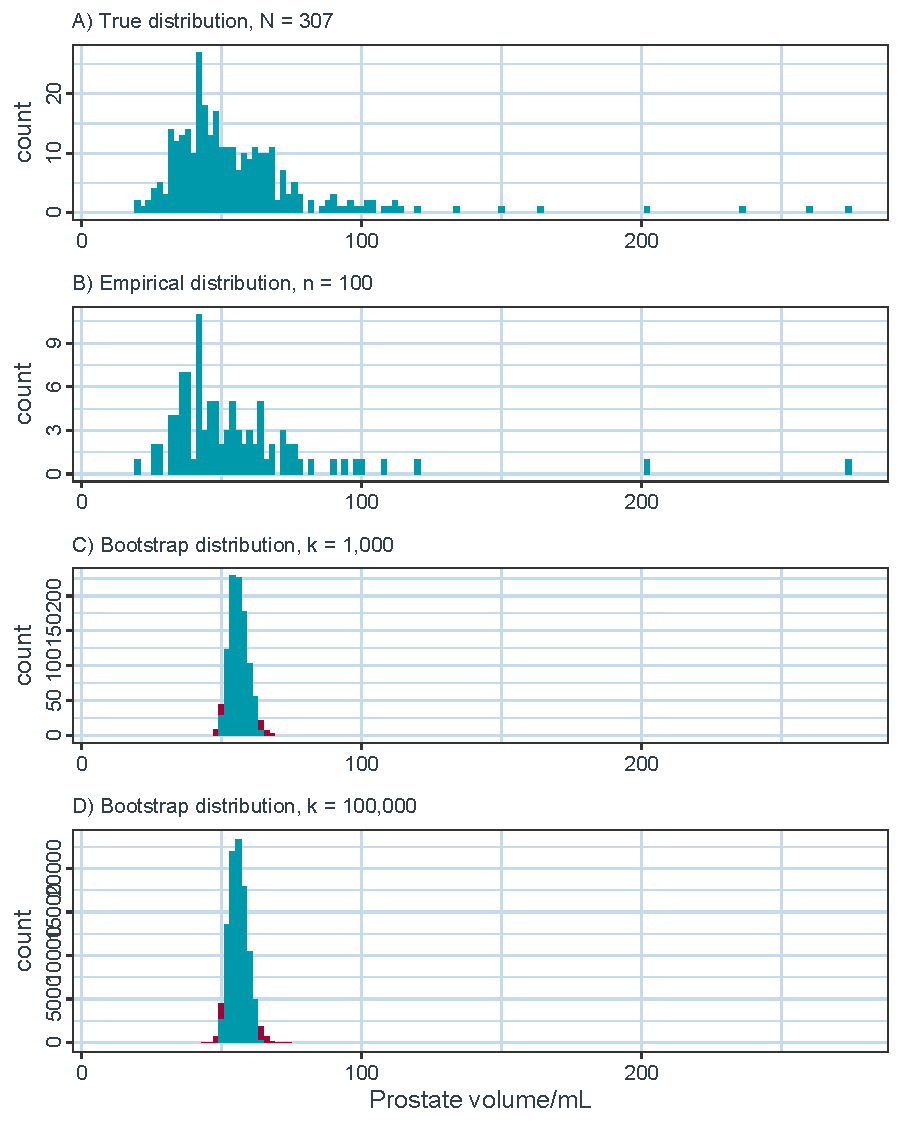
\includegraphics[keepaspectratio]{MSc_Thesis_Bookdown_files/figure-latex/prostate-vol-1.pdf}}
\caption{\label{fig:prostate-vol}Histograms demonstrating distribution of prostate volumes in patients with prostatic cancer, taken from Cata et al 2011\textsuperscript{\citeproc{ref-cata_blood_2011}{46}} via the R package \texttt{medicaldata}\textsuperscript{\citeproc{ref-medicaldata}{47}}. A) Distribution from whole study population of 307 patients with non-missing data, exhibiting right-skew. B) Distribution from random sample of 100 patients, still exhibiting right-skew. C) Bootstrap distribution generated by re-sampling 1,000 bootstrap samples from the original sample of 100 patients, right-skew less apparent. D) Bootstrap distribution generated by re-sampling 100,000 bootstrap samples from the original sample of 100 patients, approaching normality. 95\% confidence intervals are demonstrated in plots C and D by marking the 2.5th and 97.5th centiles (red-shaded areas).}
\end{figure}

\newpage

\subsection{Relevance to WME}\label{relevance-to-wme}

In current implementations of \hyperref[acronyms_WME]{WME}, the \hyperref[acronyms_WME]{WME} estimate of the causal effect (\(\hat{\beta}_{WME}\)) is calculated as described in Bowden et al\textsuperscript{\citeproc{ref-bowden_consistent_2016}{8}}, and the 95\% \hyperref[acronyms_CI]{CI} is generated separately using what is described as a bootstrapping approach. However, the implementation of this deviates from the standard bootstrapping methodology described above.

\hyperref[acronyms_CI]{CI}s for \hyperref[acronyms_WME]{WME} are generated in the following way (see \href{https://research-information.bris.ac.uk/ws/portalfiles/portal/101612595/Bowden_et_al_2016_Genetic_Epidemiology.sup_1.pdf}{Web Appendix 2} from the original paper\textsuperscript{\citeproc{ref-bowden_consistent_2016}{8}} for full code):

\begin{enumerate}
\def\labelenumi{\arabic{enumi}.}
\tightlist
\item
  Summary data (estimates of gene-exposure coefficient \(\hat{\gamma}\), gene-outcome coefficient \(\hat{\Gamma}\), and their respective standard errors) are obtained for a sample \(x\) of \(n\) genetic instruments, \(G_1, G_2...G_j...G_n\).
\item
  For each instrument \(G_j\) in \(x\), a normal distribution is created centered on the input gene-exposure coefficient estimate \(\hat{\gamma_j}\), with the \hyperref[acronyms_SD]{SD} of this distribution set equal to the \hyperref[acronyms_SE]{SE} of the estimate, \(SE({\hat{\gamma_j}})\).
\item
  Each of these normal distributions, \(\mathcal{N}(\space \hat{\gamma_j}, \space SE({\hat{\gamma_j}})\space)\), is treated as a bootstrap population for estimating the gene-exposure coefficient and standard error for its respective instrument. Each instrument is re-sampled a default of \(k = 1000\) times from its bootstrap population, forming a bootstrap distribution of \(k\) estimates of the gene-exposure coefficient for each instrument, \(\hat{\gamma}_j^{*1}, \hat{\gamma}_j^{*2}...\hat{\gamma}_j^{*k}\)
\item
  Steps \(2.\) and \(3.\) are repeated using gene-outcome coefficients and their \hyperref[acronyms_SE]{SE}s
\item
  For each instrument, a Wald estimate of causal effect, \(\hat{\beta_j} = \frac{\hat{\Gamma}_j}{\hat{\gamma}_j}\), is obtained from each of the \(k\) pairs of gene-exposure and gene-outcome coefficients, \(\hat{\beta_j}^{*1}, \hat{\beta_j}^{*2}...\hat{\beta_j}^{*k}\)
\item
  A weighted median causal estimate is calculated from each of the \(k\) sets of Wald estimates, \(\hat{\beta}_{WME}^{*1}, \hat{\beta}_{WME}^{*2}...\hat{\beta}_{WME}^{*k}\), or \((\hat{\beta}_{WME}^{*i})_{i=1}^k\)
\item
  The standard deviation of the \(k\) bootstrapped values of \((\hat{\beta}_{WME}^{*i})_{i=1}^k\) is taken as the bootstrapped standard error, \(SE^*\), of the empiric/observed \hyperref[acronyms_WME]{WME} causal estimate, \(\hat{\beta}_{WME}\). The 95\% \hyperref[acronyms_CI]{CI} is then calculated as \(\hat{\beta}_{WME} \pm 1.96  \times SE^*\)
\end{enumerate}

This approach differs from typical bootstrapping methodology in several regards. Of particular note, the instruments themselves are not re-sampled; rather, gene-exposure and gene-outcome coefficients are re-sampled from normal distributions constructed for the given set of instruments. This approach may adequately account for some random error in the estimation of these coefficients, but it does not account for the presence, distribution or magnitude of pleiotropic effects across the instruments. A re-sampling approach could account for pleiotropy-related uncertainty, but this would require re-sampling of the instruments, which is difficult to implement in practice.

Given that this method of \hyperref[acronyms_CI]{CI} generation does not account for an important source of uncertainty, it would be expected to be over-confident and produce \hyperref[acronyms_CI]{CI}s which are too narrow. Narrow \hyperref[acronyms_CI]{CI}s are less likely to include the null value, and therefore this may lead to higher rates of causality being reported when using this method, even when no true causal effect exists. As such, incorrect \hyperref[acronyms_CI]{CI} generation may therefore contribute to a higher Type 1 error rate when using \hyperref[acronyms_WME]{WME} than might otherwise be expected.

\newpage

\section{Appendix: Simulation Code}\label{appendix-sim}

\subsection{Generating Data and Models}\label{appendix-sim-gen}

The data generating model used was from Appendix 3 of Bowden et al\textsuperscript{\citeproc{ref-bowden_consistent_2016}{8}}; the relevant section describing their model is reproduced below:

\begin{quote}
\emph{``\ldots{}}
\end{quote}

\begin{quote}
\begin{equation} 
U_i = \sum^J_{j=1} \phi_jG_{ij} + \epsilon_i^U
\end{equation}
\end{quote}

\begin{quote}
\begin{equation} 
X_i = \sum^J_{j=1} \gamma_jG_{ij} + U_i + \epsilon_i^X
\end{equation}
\end{quote}

\begin{quote}
\begin{equation} 
Y_i = \sum^J_{j=1} \alpha_jG_{ij} + \beta X_i + U_i + \epsilon_i^Y
\end{equation}
\end{quote}

\begin{quote}
\emph{for participants indexed by \(i = 1, . . . , N\), and genetic instruments indexed by \(j = 1, . . . , J\).}
\end{quote}

\begin{quote}
\emph{The error terms \(\epsilon_i^U , \epsilon_i^X\) and \(\epsilon_i^Y\) were each drawn independently from standard normal distributions. The genetic effects on the exposure γj are drawn from a uniform distribution between 0.03 and 0.1. Pleiotropic effects \(\alpha_j\) and \(\phi_j\) were set to zero if the genetic instrument was a valid instrumental variable. Otherwise (with probability 0.1, 0.2, or 0.3):}
\end{quote}

\begin{quote}
\emph{1. In Scenario 1 (balanced pleiotropy, InSIDE satisfied), the \(\alpha_j\) parameter was drawn from a uniform distribution between −0.2 and 0.2.}
\end{quote}

\begin{quote}
\emph{2. In Scenario 2 (directional pleiotropy, InSIDE satisfied), the \(\alpha_j\) parameter was drawn from a uniform distribution between 0 and 0.2.}
\end{quote}

\begin{quote}
\emph{3. In Scenario 3 (directional pleiotropy, InSIDE not satisfied), the \(\phi_j\) parameter was drawn from a uniform distribution between −0.2 and 0.2.}
\end{quote}

\begin{quote}
\emph{The causal effect of the exposure on the outcome was either \(\beta X = 0\) (null causal effect) or \(\beta X = 0.1\) (positive causal effect). A total of 10 000 simulated datasets were generated for sample sizes of N = 10 000 and 20 {[}sic{]} participants. Only the summary data, that is genetic associations with the exposure and with the outcome and their standard errors as estimated by univariate regression on the genetic instruments in turn, were used by the analysis methods. In the two-sample setting, data were generated on 2N participants, and genetic associations with the exposure were estimated in the first N participants, and genetic associations with the outcome in the second N participants.''}\textsuperscript{\citeproc{ref-bowden_consistent_2016}{8}}
\end{quote}

To reproduce this model, code was written in R to generate the relevant participant level data. First, a function (\texttt{get\_simulated\_MR\_data}) was written which included parameters specified by Bowden et al, plus a toggle for random error terms to allow testing of data simulation (i.e.~\texttt{rand\_error\ =\ FALSE} sets random error/noise terms equal to zero):

\begin{Shaded}
\begin{Highlighting}[]
\CommentTok{\# Define function to create data generating model}
\CommentTok{\# Arguments/default values based on Bowden et al}
\NormalTok{get\_simulated\_MR\_data }\OtherTok{\textless{}{-}} \ControlFlowTok{function}\NormalTok{(}\AttributeTok{n\_participants =} \FunctionTok{as.integer}\NormalTok{(), }
                                  \AttributeTok{n\_instruments =} \FunctionTok{as.integer}\NormalTok{(),}
                                  \AttributeTok{n\_datasets =} \FunctionTok{as.integer}\NormalTok{(),}
                                  \AttributeTok{prop\_invalid =} \FloatTok{0.1}\NormalTok{,}
                                  \AttributeTok{causal\_effect =} \ConstantTok{TRUE}\NormalTok{,}
                                  \AttributeTok{balanced\_pleio =} \ConstantTok{TRUE}\NormalTok{,}
                                  \AttributeTok{InSIDE\_satisfied =} \ConstantTok{TRUE}\NormalTok{,}
                                  \AttributeTok{rand\_error =} \ConstantTok{TRUE}\NormalTok{,      }\CommentTok{\# remove random errors, for testing}
                                  \AttributeTok{two\_sample =} \ConstantTok{TRUE}\NormalTok{,      }\CommentTok{\# 1{-} or 2{-}sample MR toggle, for testing}
                                  \AttributeTok{beta\_val =} \FloatTok{0.1}\NormalTok{,         }\CommentTok{\# size of causal effect}
                                  \AttributeTok{allele\_freq\_min =} \FloatTok{0.4}\NormalTok{,  }\CommentTok{\# frequency of effect allele 0.01/0.99}
                                  \AttributeTok{allele\_freq\_max =} \FloatTok{0.6}\NormalTok{,  }\CommentTok{\#?0.4/0.6}
                                  \AttributeTok{gamma\_min =} \FloatTok{0.03}\NormalTok{,       }\CommentTok{\# size of genetic effects on exposure}
                                  \AttributeTok{gamma\_max =} \FloatTok{0.1}\NormalTok{,}
                                  \AttributeTok{alpha\_min =} \SpecialCharTok{{-}}\FloatTok{0.2}\NormalTok{,       }\CommentTok{\# size of pleiotropic effects on outcome}
                                  \AttributeTok{alpha\_max =} \FloatTok{0.2}\NormalTok{,}
                                  \AttributeTok{phi\_min =} \SpecialCharTok{{-}}\FloatTok{0.2}\NormalTok{,         }\CommentTok{\# size of additional pleiotropic effects}
                                  \AttributeTok{phi\_max =} \FloatTok{0.2}\NormalTok{,          }\CommentTok{\# when InSIDE not satisfied}
                                  \AttributeTok{seed =} \DecValTok{14101583}\NormalTok{)\{       }\CommentTok{\# Set seed for reproducibility}
  
  \CommentTok{\# Set seed to ensure comparability across scenarios}
  \FunctionTok{set.seed}\NormalTok{(seed)}
  
  \CommentTok{\# Initialise blank lists to receive datasets for}
  \CommentTok{\# each of:}
  \CommentTok{\#     U (vector: unmeasured confounding exposures per participant), }
  \CommentTok{\#     X (vector: exposure:outcome associations estimated per participant) }
  \CommentTok{\#     Y (vector: gene:outcome association estimated per participant), }
  \CommentTok{\#     G (Matrices: Genotype data)}
  \CommentTok{\#}
  \CommentTok{\#     gamma (vector: pleiotropic effects of each instrument on exposure)}
  \CommentTok{\#     alpha (vector: pleiotropic effects of each instrument on outcome)}
  \CommentTok{\#     phi (vector: additional pleiotropic effects of each instrument when InSIDE }
  \CommentTok{\#     assumption not satisfied)}
\NormalTok{  U\_list }\OtherTok{\textless{}{-}} \FunctionTok{list}\NormalTok{()}
\NormalTok{  X\_list }\OtherTok{\textless{}{-}} \FunctionTok{list}\NormalTok{()}
\NormalTok{  Y\_list }\OtherTok{\textless{}{-}} \FunctionTok{list}\NormalTok{()}
\NormalTok{  G\_X\_list }\OtherTok{\textless{}{-}} \FunctionTok{list}\NormalTok{()}
\NormalTok{  G\_Y\_list }\OtherTok{\textless{}{-}} \FunctionTok{list}\NormalTok{()}
  
\NormalTok{  gamma\_list }\OtherTok{\textless{}{-}} \FunctionTok{list}\NormalTok{()}
\NormalTok{  alpha\_list }\OtherTok{\textless{}{-}} \FunctionTok{list}\NormalTok{()}
\NormalTok{  phi\_list }\OtherTok{\textless{}{-}} \FunctionTok{list}\NormalTok{()}
  
  
\NormalTok{  n\_participants\_list }\OtherTok{\textless{}{-}} \FunctionTok{list}\NormalTok{()}
\NormalTok{  n\_instruments\_list }\OtherTok{\textless{}{-}} \FunctionTok{list}\NormalTok{()}
\NormalTok{  prop\_invalid\_list }\OtherTok{\textless{}{-}} \FunctionTok{list}\NormalTok{()}
\NormalTok{  beta\_val\_list }\OtherTok{\textless{}{-}} \FunctionTok{list}\NormalTok{()}
  
  
  
  \CommentTok{\# {-}{-}{-} Assign features common to all datasets {-}{-}{-} \#}
  
  \CommentTok{\# size of causal effect}
\NormalTok{  beta }\OtherTok{\textless{}{-}} \FunctionTok{if\_else}\NormalTok{(causal\_effect }\SpecialCharTok{==} \ConstantTok{TRUE}\NormalTok{, }
\NormalTok{                  beta\_val,}
                  \DecValTok{0}\NormalTok{)}
  
  \CommentTok{\# create vector of participant indices for 1st n participants}
  \CommentTok{\# i.e. participants used for estimating gene:exposure coefficient}
\NormalTok{  sample\_1\_ref }\OtherTok{\textless{}{-}} \DecValTok{1}\SpecialCharTok{:}\NormalTok{n\_participants        }
  
  
  \CommentTok{\# Default is to estimate gene:outcome coefficient from different sample}
  \CommentTok{\# to gene:exposure coefficient (i.e. simulating 2{-}sample MR)}
  \CommentTok{\# two\_sample == FALSE toggles to single sample for testing simulation}
  \FunctionTok{ifelse}\NormalTok{(two\_sample }\SpecialCharTok{==} \ConstantTok{FALSE}\NormalTok{,}
\NormalTok{         sample\_2\_ref }\OtherTok{\textless{}{-}}\NormalTok{ sample\_1\_ref, }\CommentTok{\# 1 sample MR}
\NormalTok{         sample\_2\_ref }\OtherTok{\textless{}{-}}\NormalTok{ (n\_participants}\SpecialCharTok{+}\DecValTok{1}\NormalTok{)}\SpecialCharTok{:}\NormalTok{(}\DecValTok{2}\SpecialCharTok{*}\NormalTok{n\_participants)) }\CommentTok{\# 2 sample MR}
  
  \CommentTok{\# {-}{-}{-} Set characteristics for each genetic instrument {-}{-}{-} \# }
  
  \CommentTok{\# Set genetic effects of each instrument on the exposure,}
  \CommentTok{\# drawn from uniform distribution, min/max as per Bowden }
  \CommentTok{\# et al}
\NormalTok{  gamma\_vect }\OtherTok{\textless{}{-}} \FunctionTok{runif}\NormalTok{(}\AttributeTok{n =}\NormalTok{ n\_instruments,}
                      \AttributeTok{min =}\NormalTok{ gamma\_min,}
                      \AttributeTok{max =}\NormalTok{ gamma\_max)}
  
  
  
  \CommentTok{\# Set which instruments invalid, 0 = valid, 1 = invalid}
\NormalTok{  invalid\_instrument\_vect }\OtherTok{\textless{}{-}} \FunctionTok{rbinom}\NormalTok{(}\AttributeTok{n =}\NormalTok{ n\_instruments,}
                                    \AttributeTok{size =} \DecValTok{1}\NormalTok{, }
                                    \AttributeTok{prob =}\NormalTok{ prop\_invalid)}
  
  
  \CommentTok{\# Probability of effect allele set per dataset  }
  \CommentTok{\# for each instrument, default value set at  }
  \CommentTok{\# random between 0.4{-}0.6 (i.e. both effect +}
  \CommentTok{\# reference are common alleles)}
\NormalTok{  allele\_freq\_vect }\OtherTok{\textless{}{-}} \FunctionTok{runif}\NormalTok{(}\AttributeTok{n =}\NormalTok{ n\_instruments,}
                            \AttributeTok{min =}\NormalTok{ allele\_freq\_min,}
                            \AttributeTok{max =}\NormalTok{ allele\_freq\_max)}
  
  \CommentTok{\# Set pleiotropic effects on outcome, Scenarios and }
  \CommentTok{\# min/max from Bowden et al}
\NormalTok{  alpha\_vect }\OtherTok{\textless{}{-}} \FunctionTok{double}\NormalTok{() }\CommentTok{\# Pleiotropic effects of instruments on outcome}
\NormalTok{  phi\_vect }\OtherTok{\textless{}{-}} \FunctionTok{double}\NormalTok{() }\CommentTok{\# Pleiotropic effects of confounders on outcome}
  
  
  \ControlFlowTok{for}\NormalTok{(j }\ControlFlowTok{in} \DecValTok{1}\SpecialCharTok{:}\NormalTok{n\_instruments)\{}
    \FunctionTok{ifelse}\NormalTok{(invalid\_instrument\_vect[j] }\SpecialCharTok{==} \DecValTok{0}\NormalTok{, }\CommentTok{\# alpha = 0 if valid}
\NormalTok{           alpha\_vect[j] }\OtherTok{\textless{}{-}} \DecValTok{0}\NormalTok{,}
           \FunctionTok{ifelse}\NormalTok{(balanced\_pleio }\SpecialCharTok{==} \ConstantTok{TRUE}\NormalTok{,}
\NormalTok{                  alpha\_vect[j] }\OtherTok{\textless{}{-}} \FunctionTok{runif}\NormalTok{(}\AttributeTok{n =} \DecValTok{1}\NormalTok{, }\CommentTok{\# balanced}
                                         \AttributeTok{min =}\NormalTok{ alpha\_min,}
                                         \AttributeTok{max =}\NormalTok{ alpha\_max),}
\NormalTok{                  alpha\_vect[j] }\OtherTok{\textless{}{-}} \FunctionTok{runif}\NormalTok{(}\AttributeTok{n =} \DecValTok{1}\NormalTok{, }\CommentTok{\# directional}
                                         \AttributeTok{min =} \DecValTok{0}\NormalTok{,}
                                         \AttributeTok{max =}\NormalTok{ alpha\_max)}
\NormalTok{           )}
\NormalTok{    )}
    
    
    \CommentTok{\# Assign default phi = 0 unless directional pleiotropy \& }
    \CommentTok{\# InSIDE assumption not satisfied \& genetic instrument invalid}
    \ControlFlowTok{if}\NormalTok{(balanced\_pleio }\SpecialCharTok{==} \ConstantTok{FALSE} \SpecialCharTok{\&}\NormalTok{ InSIDE\_satisfied }\SpecialCharTok{==} \ConstantTok{FALSE}\NormalTok{)\{}
      \FunctionTok{ifelse}\NormalTok{(invalid\_instrument\_vect[j] }\SpecialCharTok{==} \DecValTok{0}\NormalTok{,}
\NormalTok{             phi\_vect[j] }\OtherTok{\textless{}{-}} \DecValTok{0}\NormalTok{,}
\NormalTok{             phi\_vect[j] }\OtherTok{\textless{}{-}} \FunctionTok{runif}\NormalTok{(}\AttributeTok{n =} \DecValTok{1}\NormalTok{,}
                                  \AttributeTok{min =}\NormalTok{ phi\_min,}
                                  \AttributeTok{max =}\NormalTok{ phi\_max)}
\NormalTok{      )}
      
\NormalTok{    \}}
    \ControlFlowTok{else}\NormalTok{\{}
\NormalTok{      phi\_vect[j] }\OtherTok{\textless{}{-}} \DecValTok{0}
\NormalTok{    \}}
\NormalTok{  \}}
  
  \CommentTok{\# Re{-}set seed to ensure consistency across datasets}
  \CommentTok{\# N.B. above two if/ifelse statements cause de{-}sync }
  \CommentTok{\# of number of randomised functions between valid/invalid}
  \FunctionTok{set.seed}\NormalTok{(seed)}
  
  \CommentTok{\# {-}{-}{-} Create separate datasets {-}{-}{-} \#}
  
  \CommentTok{\# Create N datasets by simulating genotype matrices with}
  \CommentTok{\# 1 row per participant, 1 column per genetic instrument}
  \CommentTok{\# Use these to estimate U, X + Y}
  
  \ControlFlowTok{for}\NormalTok{(n }\ControlFlowTok{in} \DecValTok{1}\SpecialCharTok{:}\NormalTok{n\_datasets)\{}
    
    \CommentTok{\# {-}{-}{-} Create matrix of genotypes {-}{-}{-} \#}
    
    \CommentTok{\# Assign genotypes by sampling from binomial distribution}
    \CommentTok{\# twice (as two alleles) per participant with probability}
    \CommentTok{\# equal to frequency of effect allele}
    \CommentTok{\# Create twice as many genotypes as participants in sample}
    \CommentTok{\# to simulate 2 sample MR, i.e. first half used to estimate}
    \CommentTok{\# Gene:Exposure, second half used to estimate Gene:Outcome}
    
    \CommentTok{\# Matrix where columns are instruments, rows are participants}
    \CommentTok{\# Values 0, 1 or 2}
    \CommentTok{\# 0 = reference, i.e. zero effect alleles, }
    \CommentTok{\# 1 = 1 effect allele, 2 = 2 effect alleles }
    
\NormalTok{    G\_mat }\OtherTok{\textless{}{-}} \FunctionTok{matrix}\NormalTok{(}\FunctionTok{rbinom}\NormalTok{(}\AttributeTok{n =} \DecValTok{2} \SpecialCharTok{*}\NormalTok{ n\_participants }\SpecialCharTok{*}\NormalTok{ n\_instruments,}
                           \AttributeTok{size =} \DecValTok{2}\NormalTok{,}
                           \AttributeTok{prob =} \FunctionTok{rep}\NormalTok{(allele\_freq\_vect, }\DecValTok{2} \SpecialCharTok{*}\NormalTok{ n\_participants)),}
                    \AttributeTok{nrow =} \DecValTok{2} \SpecialCharTok{*}\NormalTok{ n\_participants,}
                    \AttributeTok{ncol =}\NormalTok{ n\_instruments,}
                    \AttributeTok{byrow =} \ConstantTok{TRUE}\NormalTok{)}
    
    
    \CommentTok{\# Create error terms for U, X + Y per participant,}
    \CommentTok{\# each drawn from standard normal distribution}
    \CommentTok{\# unless random error turned off (for testing)}
    
    \FunctionTok{ifelse}\NormalTok{(rand\_error }\SpecialCharTok{==} \ConstantTok{TRUE}\NormalTok{,}
\NormalTok{           U\_epsilon\_vect }\OtherTok{\textless{}{-}} \FunctionTok{rnorm}\NormalTok{(}\AttributeTok{n =} \DecValTok{2} \SpecialCharTok{*}\NormalTok{ n\_participants),}
\NormalTok{           U\_epsilon\_vect }\OtherTok{\textless{}{-}} \FunctionTok{rep}\NormalTok{(}\DecValTok{0}\NormalTok{, }\DecValTok{2} \SpecialCharTok{*}\NormalTok{ n\_participants))}
    
    \FunctionTok{ifelse}\NormalTok{(rand\_error }\SpecialCharTok{==} \ConstantTok{TRUE}\NormalTok{,}
\NormalTok{           X\_epsilon\_vect }\OtherTok{\textless{}{-}} \FunctionTok{rnorm}\NormalTok{(}\AttributeTok{n =}\NormalTok{ n\_participants),}
\NormalTok{           X\_epsilon\_vect }\OtherTok{\textless{}{-}} \FunctionTok{rep}\NormalTok{(}\DecValTok{0}\NormalTok{, n\_participants))}
    
    \FunctionTok{ifelse}\NormalTok{(rand\_error }\SpecialCharTok{==} \ConstantTok{TRUE}\NormalTok{,}
\NormalTok{           Y\_epsilon\_vect }\OtherTok{\textless{}{-}} \FunctionTok{rnorm}\NormalTok{(}\AttributeTok{n =}\NormalTok{ n\_participants),}
\NormalTok{           Y\_epsilon\_vect }\OtherTok{\textless{}{-}} \FunctionTok{rep}\NormalTok{(}\DecValTok{0}\NormalTok{, n\_participants))}
    
    
    \CommentTok{\# {-}{-}{-} Combine Gene matrix/parameters to recreate model {-}{-}{-} \#}
    
    \CommentTok{\# Create vectors of estimates for U, X and Y per individual,}
    \CommentTok{\# i.e. Ui, Xi and Yi. Uses matrix inner product operator " \%*\%" }
    \CommentTok{\# https://stackoverflow.com/questions/22060515/the{-}r{-}operator }
    \CommentTok{\# http://matrixmultiplication.xyz/}
    
    \CommentTok{\#     U (vector: unmeasured confounding exposures per participant), }
    \CommentTok{\#     X (vector: exposure:outcome associations estimated per participant) }
    \CommentTok{\#     Y (vector: gene:outcome association estimated per participant) }
    
\NormalTok{    Ui\_vect }\OtherTok{\textless{}{-}}\NormalTok{  G\_mat }\SpecialCharTok{\%*\%}\NormalTok{ phi\_vect }\SpecialCharTok{+}\NormalTok{ U\_epsilon\_vect}
    
\NormalTok{    Xi\_vect }\OtherTok{\textless{}{-}}\NormalTok{  G\_mat[sample\_1\_ref, ] }\SpecialCharTok{\%*\%}\NormalTok{ gamma\_vect }\SpecialCharTok{+} 
\NormalTok{      Ui\_vect[sample\_1\_ref, ] }\SpecialCharTok{+} 
\NormalTok{      X\_epsilon\_vect}
    
\NormalTok{    Yi\_vect }\OtherTok{\textless{}{-}}\NormalTok{  G\_mat[sample\_2\_ref, ] }\SpecialCharTok{\%*\%}\NormalTok{ alpha\_vect }\SpecialCharTok{+} 
\NormalTok{      beta }\SpecialCharTok{*}\NormalTok{ Xi\_vect }\SpecialCharTok{+} 
\NormalTok{      Ui\_vect[sample\_2\_ref, ] }\SpecialCharTok{+} 
\NormalTok{      Y\_epsilon\_vect}
    
    
    \CommentTok{\# Add vectors of estimates from this dataset to lists of }
    \CommentTok{\# estimates from all datasets}
\NormalTok{    U\_list[[n]] }\OtherTok{\textless{}{-}}\NormalTok{ Ui\_vect}
    
\NormalTok{    X\_list[[n]] }\OtherTok{\textless{}{-}}\NormalTok{ Xi\_vect}
    
\NormalTok{    Y\_list[[n]] }\OtherTok{\textless{}{-}}\NormalTok{ Yi\_vect}
    
\NormalTok{    G\_X\_list[[n]] }\OtherTok{\textless{}{-}}\NormalTok{ G\_mat[sample\_1\_ref, ]}
    
\NormalTok{    G\_Y\_list[[n]] }\OtherTok{\textless{}{-}}\NormalTok{ G\_mat[sample\_2\_ref, ]}
    
    
    \CommentTok{\# Include actual parameter values generated for simulation }
\NormalTok{    alpha\_list[[n]] }\OtherTok{\textless{}{-}}\NormalTok{ alpha\_vect}
    
\NormalTok{    gamma\_list[[n]] }\OtherTok{\textless{}{-}}\NormalTok{ gamma\_vect}
    
\NormalTok{    phi\_list[[n]] }\OtherTok{\textless{}{-}}\NormalTok{ phi\_vect}
    
    \CommentTok{\# Include inputs for reference/testing }
\NormalTok{    n\_participants\_list[[n]] }\OtherTok{\textless{}{-}}\NormalTok{ n\_participants}
\NormalTok{    n\_instruments\_list[[n]] }\OtherTok{\textless{}{-}}\NormalTok{ n\_instruments}
\NormalTok{    prop\_invalid\_list[[n]] }\OtherTok{\textless{}{-}}\NormalTok{ prop\_invalid}
\NormalTok{    beta\_val\_list[[n]] }\OtherTok{\textless{}{-}}\NormalTok{ beta\_val}
    
    
\NormalTok{  \}}
  
  
  
  \CommentTok{\# {-}{-}{-} Combine all outputs to return {-}{-}{-} \#}
  
\NormalTok{  combined\_list }\OtherTok{\textless{}{-}} \FunctionTok{list}\NormalTok{(}\AttributeTok{U =}\NormalTok{ U\_list,         }\CommentTok{\# Estimates }
                        \AttributeTok{X =}\NormalTok{ X\_list, }
                        \AttributeTok{Y =}\NormalTok{ Y\_list,}
                        
                        \AttributeTok{G\_X =}\NormalTok{ G\_X\_list,     }\CommentTok{\# Genotypes of 1st sample}
                        \AttributeTok{G\_Y =}\NormalTok{ G\_Y\_list,     }\CommentTok{\# Genotypes of 2nd sample}
                        
                        \AttributeTok{alpha =}\NormalTok{ alpha\_list, }\CommentTok{\# Actual values for validating simulation}
                        \AttributeTok{gamma =}\NormalTok{ gamma\_list,}
                        \AttributeTok{phi =}\NormalTok{ phi\_list,}
                        
                        \AttributeTok{n\_participants =}\NormalTok{ n\_participants\_list, }\CommentTok{\# Inputs}
                        \AttributeTok{n\_instruments =}\NormalTok{ n\_instruments\_list,}
                        \AttributeTok{prop\_invalid =}\NormalTok{ prop\_invalid\_list,}
                        \AttributeTok{beta\_val =}\NormalTok{ beta\_val\_list}
\NormalTok{  )}
  
  \FunctionTok{return}\NormalTok{(combined\_list)}
\NormalTok{\}}
\end{Highlighting}
\end{Shaded}

This initial simulation function generated data in the following format:

\begin{Shaded}
\begin{Highlighting}[]
\CommentTok{\# Check data produced in expected format}
\CommentTok{\#set.seed(1701)}
\NormalTok{test\_data\_sim }\OtherTok{\textless{}{-}} \FunctionTok{get\_simulated\_MR\_data}\NormalTok{(}\AttributeTok{n\_participants =} \DecValTok{1000}\NormalTok{,}
                                       \AttributeTok{n\_instruments =} \DecValTok{25}\NormalTok{,}
                                       \AttributeTok{n\_datasets =} \DecValTok{2}\NormalTok{,}
                                       \AttributeTok{prop\_invalid =} \FloatTok{0.3}\NormalTok{,}
                                       \AttributeTok{rand\_error =} \ConstantTok{FALSE}\NormalTok{,}
                                       \AttributeTok{causal\_effect =} \ConstantTok{TRUE}\NormalTok{,}
                                       \AttributeTok{balanced\_pleio =} \ConstantTok{TRUE}\NormalTok{,}
                                       \AttributeTok{InSIDE\_satisfied =} \ConstantTok{TRUE}\NormalTok{)}

\FunctionTok{str}\NormalTok{(test\_data\_sim)}
\end{Highlighting}
\end{Shaded}

\begin{verbatim}
## List of 12
##  $ U             :List of 2
##   ..$ : num [1:2000, 1] 0 0 0 0 0 0 0 0 0 0 ...
##   ..$ : num [1:2000, 1] 0 0 0 0 0 0 0 0 0 0 ...
##  $ X             :List of 2
##   ..$ : num [1:1000, 1] 1.59 1.29 1.02 1.89 1.49 ...
##   ..$ : num [1:1000, 1] 1.85 1.84 2.18 1.16 1.44 ...
##  $ Y             :List of 2
##   ..$ : num [1:1000, 1] 0.0704 0.1351 0.1589 0.0944 0.0161 ...
##   ..$ : num [1:1000, 1] 0.59017 0.10039 0.00743 0.27896 0.27746 ...
##  $ G_X           :List of 2
##   ..$ : int [1:1000, 1:25] 2 0 1 2 1 0 1 0 0 2 ...
##   ..$ : int [1:1000, 1:25] 0 1 2 1 1 1 0 2 0 2 ...
##  $ G_Y           :List of 2
##   ..$ : int [1:1000, 1:25] 1 1 0 1 2 0 1 0 1 2 ...
##   ..$ : int [1:1000, 1:25] 1 1 1 1 0 1 2 0 2 0 ...
##  $ alpha         :List of 2
##   ..$ : num [1:25] 0 0 0.1157 0 -0.0634 ...
##   ..$ : num [1:25] 0 0 0.1157 0 -0.0634 ...
##  $ gamma         :List of 2
##   ..$ : num [1:25] 0.0938 0.0808 0.0755 0.0342 0.0443 ...
##   ..$ : num [1:25] 0.0938 0.0808 0.0755 0.0342 0.0443 ...
##  $ phi           :List of 2
##   ..$ : num [1:25] 0 0 0 0 0 0 0 0 0 0 ...
##   ..$ : num [1:25] 0 0 0 0 0 0 0 0 0 0 ...
##  $ n_participants:List of 2
##   ..$ : num 1000
##   ..$ : num 1000
##  $ n_instruments :List of 2
##   ..$ : num 25
##   ..$ : num 25
##  $ prop_invalid  :List of 2
##   ..$ : num 0.3
##   ..$ : num 0.3
##  $ beta_val      :List of 2
##   ..$ : num 0.1
##   ..$ : num 0.1
\end{verbatim}

A function (\texttt{get\_models}) was then written to create linear models from each dataset generated as per Bowden et al:

\begin{Shaded}
\begin{Highlighting}[]
\CommentTok{\# Create plotting tibble with Mean/SD X + Y grouped by}
\CommentTok{\# Dataset + instrument}
\NormalTok{get\_models }\OtherTok{\textless{}{-}} \ControlFlowTok{function}\NormalTok{(sim)\{}
  
\NormalTok{  output\_list }\OtherTok{\textless{}{-}} \FunctionTok{list}\NormalTok{()}
  
  \CommentTok{\# Create linear models per dataset to get coefficients}
  \CommentTok{\# for gene:exposure association (coeff\_G\_X) and gene:outcome}
  \CommentTok{\# association (coeff\_G\_Y)}
  \ControlFlowTok{for}\NormalTok{(dataset }\ControlFlowTok{in} \DecValTok{1}\SpecialCharTok{:}\FunctionTok{length}\NormalTok{(sim}\SpecialCharTok{$}\NormalTok{X))\{}
    
\NormalTok{    X }\OtherTok{\textless{}{-}}\NormalTok{ sim}\SpecialCharTok{$}\NormalTok{X[[dataset]]}
\NormalTok{    Y }\OtherTok{\textless{}{-}}\NormalTok{ sim}\SpecialCharTok{$}\NormalTok{Y[[dataset]]}
\NormalTok{    Instruments\_X }\OtherTok{\textless{}{-}}\NormalTok{ sim}\SpecialCharTok{$}\NormalTok{G\_X[[dataset]]}
\NormalTok{    Instruments\_Y }\OtherTok{\textless{}{-}}\NormalTok{ sim}\SpecialCharTok{$}\NormalTok{G\_Y[[dataset]]}
    
\NormalTok{    alpha }\OtherTok{\textless{}{-}}\NormalTok{ sim}\SpecialCharTok{$}\NormalTok{alpha[[dataset]]}
\NormalTok{    gamma }\OtherTok{\textless{}{-}}\NormalTok{ sim}\SpecialCharTok{$}\NormalTok{gamma[[dataset]]}
\NormalTok{    phi }\OtherTok{\textless{}{-}}\NormalTok{ sim}\SpecialCharTok{$}\NormalTok{phi[[dataset]]}
\NormalTok{    beta }\OtherTok{\textless{}{-}}\NormalTok{ sim}\SpecialCharTok{$}\NormalTok{beta\_val[[dataset]]}
\NormalTok{    prop\_invalid }\OtherTok{\textless{}{-}}\NormalTok{ sim}\SpecialCharTok{$}\NormalTok{prop\_invalid[[dataset]]}
\NormalTok{    n\_instruments }\OtherTok{\textless{}{-}}\NormalTok{ sim}\SpecialCharTok{$}\NormalTok{n\_instruments[[dataset]]}
\NormalTok{    n\_participants}\OtherTok{\textless{}{-}}\NormalTok{ sim}\SpecialCharTok{$}\NormalTok{n\_participants[[dataset]]}
    
    
    \CommentTok{\# Model for gene:exposure}
\NormalTok{    X\_lm }\OtherTok{\textless{}{-}} \FunctionTok{lm}\NormalTok{(X }\SpecialCharTok{\textasciitilde{}} \DecValTok{0} \SpecialCharTok{+}\NormalTok{ Instruments\_X)}
\NormalTok{    coeff\_G\_X\_vect }\OtherTok{\textless{}{-}} \FunctionTok{coef}\NormalTok{(}\FunctionTok{summary}\NormalTok{(X\_lm))[}\DecValTok{1}\SpecialCharTok{:}\NormalTok{(}\FunctionTok{ncol}\NormalTok{(Instruments\_X)), }\DecValTok{1}\NormalTok{]}
\NormalTok{    SE\_coeff\_G\_X\_vect }\OtherTok{\textless{}{-}} \FunctionTok{coef}\NormalTok{(}\FunctionTok{summary}\NormalTok{(X\_lm))[}\DecValTok{1}\SpecialCharTok{:}\NormalTok{(}\FunctionTok{ncol}\NormalTok{(Instruments\_X)), }\DecValTok{2}\NormalTok{]}
    
\NormalTok{    R2\_stat }\OtherTok{\textless{}{-}} \FunctionTok{summary}\NormalTok{(}\FunctionTok{lm}\NormalTok{(X }\SpecialCharTok{\textasciitilde{}}\NormalTok{ Instruments\_X))}\SpecialCharTok{$}\NormalTok{r.squared}
\NormalTok{    F\_stat }\OtherTok{\textless{}{-}} \FunctionTok{summary}\NormalTok{(}\FunctionTok{lm}\NormalTok{(X }\SpecialCharTok{\textasciitilde{}}\NormalTok{ Instruments\_X))}\SpecialCharTok{$}\NormalTok{fstatistic[[}\DecValTok{1}\NormalTok{]]}
    
    
    \CommentTok{\# Model for gene:outcome}
\NormalTok{    Y\_lm }\OtherTok{\textless{}{-}} \FunctionTok{lm}\NormalTok{(Y }\SpecialCharTok{\textasciitilde{}} \DecValTok{0} \SpecialCharTok{+}\NormalTok{ Instruments\_Y)}
\NormalTok{    coeff\_G\_Y\_vect }\OtherTok{\textless{}{-}} \FunctionTok{coef}\NormalTok{(}\FunctionTok{summary}\NormalTok{(Y\_lm))[}\DecValTok{1}\SpecialCharTok{:}\NormalTok{(}\FunctionTok{ncol}\NormalTok{(Instruments\_Y)), }\DecValTok{1}\NormalTok{] }
\NormalTok{    SE\_coeff\_G\_Y\_vect }\OtherTok{\textless{}{-}} \FunctionTok{coef}\NormalTok{(}\FunctionTok{summary}\NormalTok{(Y\_lm))[}\DecValTok{1}\SpecialCharTok{:}\NormalTok{(}\FunctionTok{ncol}\NormalTok{(Instruments\_Y)), }\DecValTok{2}\NormalTok{]}
    
\NormalTok{    output\_list[[dataset]] }\OtherTok{\textless{}{-}} \FunctionTok{as\_tibble}\NormalTok{(}\FunctionTok{list}\NormalTok{(}\AttributeTok{dataset =}\NormalTok{ dataset,}
                                             \AttributeTok{Instrument =} \FunctionTok{c}\NormalTok{(}\DecValTok{1}\SpecialCharTok{:}\FunctionTok{ncol}\NormalTok{(Instruments\_X)),}
                                             \AttributeTok{coeff\_G\_X =}\NormalTok{ coeff\_G\_X\_vect,}
                                             \AttributeTok{coeff\_G\_X\_SE =}\NormalTok{ SE\_coeff\_G\_X\_vect,}
                                             \AttributeTok{gamma =}\NormalTok{ gamma,}
                                             \AttributeTok{F\_stat =}\NormalTok{ F\_stat,}
                                             \AttributeTok{R2\_stat =}\NormalTok{ R2\_stat,}
                                             \AttributeTok{coeff\_G\_Y =}\NormalTok{ coeff\_G\_Y\_vect,}
                                             \AttributeTok{coeff\_G\_Y\_SE =}\NormalTok{ SE\_coeff\_G\_Y\_vect,}
                                             \AttributeTok{alpha =}\NormalTok{ alpha,}
                                             \AttributeTok{phi =}\NormalTok{ phi,}
                                             \AttributeTok{beta =}\NormalTok{ beta,}
                                             \AttributeTok{prop\_invalid =}\NormalTok{ prop\_invalid,}
                                             \AttributeTok{n\_instruments =}\NormalTok{ n\_instruments,}
                                             \AttributeTok{n\_participants =}\NormalTok{ n\_participants),}
                                        \AttributeTok{.name\_repair =} \StringTok{"unique"}\NormalTok{)}
\NormalTok{  \}}
  
  \FunctionTok{return}\NormalTok{(output\_list)}
  
\NormalTok{\}  }
\end{Highlighting}
\end{Shaded}

These models generated estimates of the coefficient of gene-exposure association (\texttt{coeff\_G\_X}), coefficient of gene-outcome association (\texttt{coeff\_G\_Y}), and the relevant standard errors of these estimates. The values of parameters inputted were also returned to aid in further testing of data/model generation, i.e.~actual gene-exposure associations (\texttt{gamma}), pleiotropic effects of invalid instruments (\texttt{alpha}), additional pleiotropic effects when \hyperref[acronyms_InSIDE]{InSIDE} assumption not satified (\texttt{phi}), causal effect of exposure on outcome (\texttt{beta}) and the proportion of invalid genetic instruments with pleiotropic effects on the outcome (\texttt{prop\_invalid}).

\begin{Shaded}
\begin{Highlighting}[]
\NormalTok{test\_extract\_model }\OtherTok{\textless{}{-}} \FunctionTok{get\_models}\NormalTok{(test\_data\_sim)}

\FunctionTok{summary}\NormalTok{(test\_extract\_model[[}\DecValTok{1}\NormalTok{]])}
\end{Highlighting}
\end{Shaded}

\begin{verbatim}
##     dataset    Instrument   coeff_G_X        coeff_G_X_SE           gamma             F_stat         
##  Min.   :1   Min.   : 1   Min.   :0.03419   Min.   :6.659e-17   Min.   :0.03419   Min.   :6.224e+27  
##  1st Qu.:1   1st Qu.: 7   1st Qu.:0.05645   1st Qu.:6.807e-17   1st Qu.:0.05645   1st Qu.:6.224e+27  
##  Median :1   Median :13   Median :0.06823   Median :6.873e-17   Median :0.06823   Median :6.224e+27  
##  Mean   :1   Mean   :13   Mean   :0.06791   Mean   :6.889e-17   Mean   :0.06791   Mean   :6.224e+27  
##  3rd Qu.:1   3rd Qu.:19   3rd Qu.:0.08594   3rd Qu.:6.935e-17   3rd Qu.:0.08594   3rd Qu.:6.224e+27  
##  Max.   :1   Max.   :25   Max.   :0.09379   Max.   :7.313e-17   Max.   :0.09379   Max.   :6.224e+27  
##     R2_stat    coeff_G_Y          coeff_G_Y_SE          alpha                phi         beta    
##  Min.   :1   Min.   :-0.109067   Min.   :0.001550   Min.   :-0.115363   Min.   :0   Min.   :0.1  
##  1st Qu.:1   1st Qu.: 0.004951   1st Qu.:0.001579   1st Qu.: 0.000000   1st Qu.:0   1st Qu.:0.1  
##  Median :1   Median : 0.006555   Median :0.001591   Median : 0.000000   Median :0   Median :0.1  
##  Mean   :1   Mean   : 0.013297   Mean   :0.001598   Mean   : 0.006717   Mean   :0   Mean   :0.1  
##  3rd Qu.:1   3rd Qu.: 0.008890   3rd Qu.:0.001624   3rd Qu.: 0.000000   3rd Qu.:0   3rd Qu.:0.1  
##  Max.   :1   Max.   : 0.162629   Max.   :0.001653   Max.   : 0.156224   Max.   :0   Max.   :0.1  
##   prop_invalid n_instruments n_participants
##  Min.   :0.3   Min.   :25    Min.   :1000  
##  1st Qu.:0.3   1st Qu.:25    1st Qu.:1000  
##  Median :0.3   Median :25    Median :1000  
##  Mean   :0.3   Mean   :25    Mean   :1000  
##  3rd Qu.:0.3   3rd Qu.:25    3rd Qu.:1000  
##  Max.   :0.3   Max.   :25    Max.   :1000
\end{verbatim}

\newpage

\subsection{Testing Generation of Data and Models}\label{appendix-sim-test}

A series of test plots were used to verify that data were simulated as intended under the various conditions specified by input parameters. Test plots were not created for the parameters \texttt{n\_participants}, \texttt{n\_instruments} or \texttt{n\_datasets}, as the functioning of these parameters could be readily inferred from the structure of the datasets outputted, as above.

\subsubsection{Proportion of Invalid Instruments}\label{proportion-of-invalid-instruments}

\leavevmode\newline The \texttt{prop\_invalid} parameter specifies the proportion of invalid genetic instruments simulated, i.e.~the proportion of genetic instruments affecting the outcome via direct/pleiotropic effects, and thus not solely via the exposure of interest. If simulated correctly, increasing the value of \texttt{prop\_invalid} should increase the number of instruments with pleiotropic effects, i.e.~instruments with \texttt{alpha} \(\ne\) 0. With random error terms set to 0 and no causal effect present (i.e.~\texttt{rand\_error\ =\ FALSE} and \texttt{causal\_effect\ =\ FALSE}), the estimated gene-outcome coefficient estimated using any given instrument will equal the pleiotropic effects of that instrument (i.e.~\texttt{coeff\_G\_Y\ =\ alpha}), and therefore will only be non-zero for invalid instruments with non-zero pleiotropic effects on the outcome . Plotting \texttt{coeff\_G\_Y} against \texttt{alpha} for simulated data with no causal effect or random error should therefore yield a graph where

\begin{itemize}
\tightlist
\item
  For valid instruments: gene-outcome coefficient = alpha = 0
\item
  For invalid instruments: gene-outcome coefficient = alpha \(\ne\) 0, with values spread uniformly between \texttt{alpha\_min} and \texttt{alpha\_max}
\end{itemize}

\pandocbounded{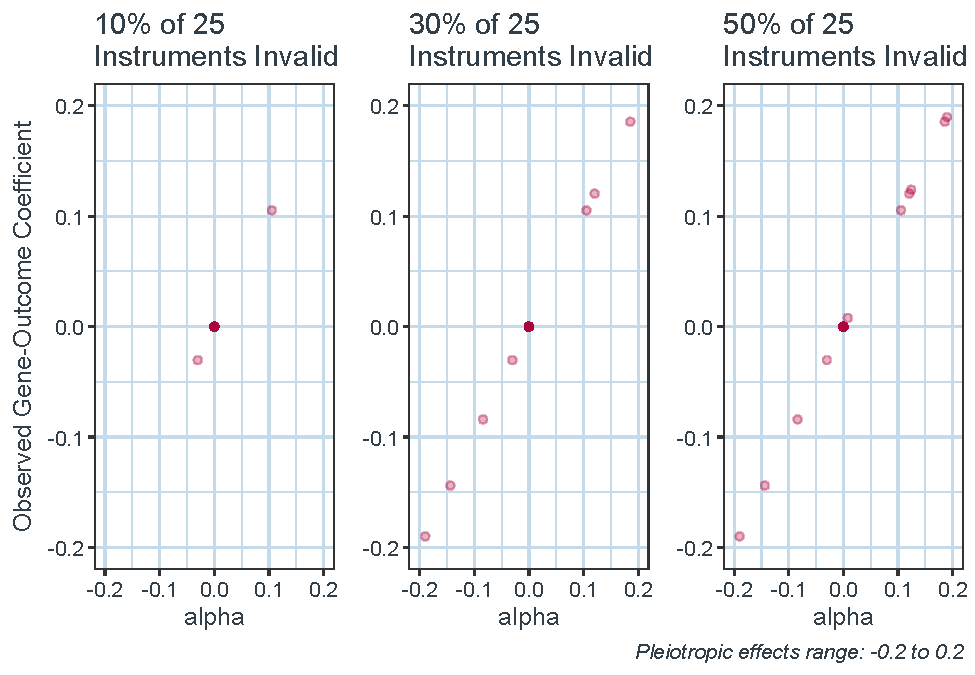
\includegraphics[keepaspectratio]{MSc_Thesis_Bookdown_files/figure-latex/test-plot-prop-invalid-1.pdf}}

\newpage

Similarly, with random error terms set to 0 (\texttt{rand\_error\ =\ FALSE}) and no causal effect present (\texttt{causal\_effect\ =\ FALSE}), gene-exposure coefficients estimated for each instrument should exactly match the actual values simulated, i.e.~\texttt{coeff\_G\_X\ =\ gamma} for all instruments:

\pandocbounded{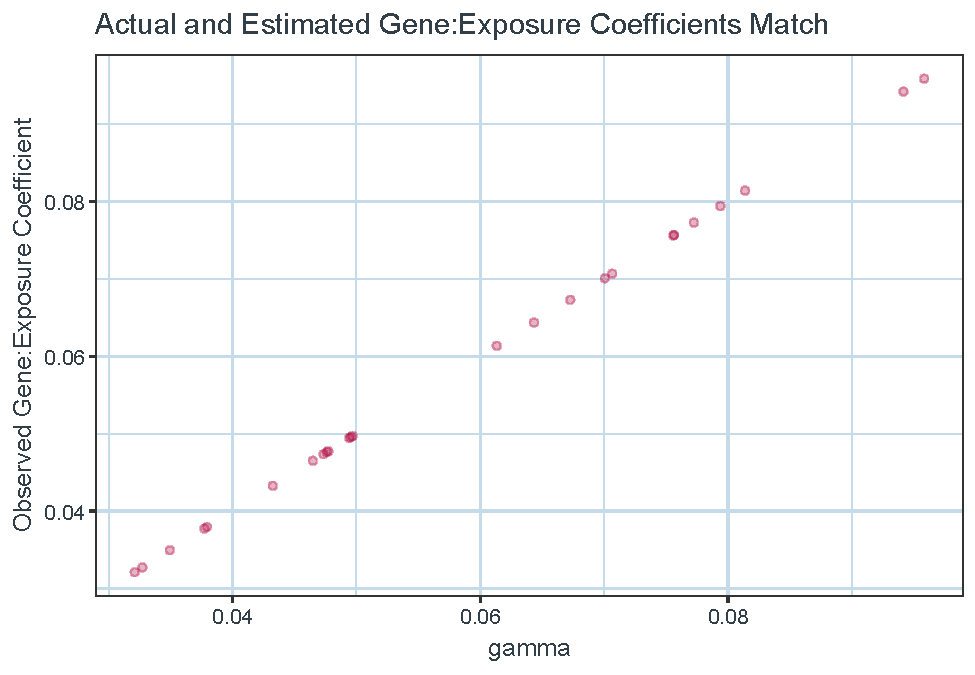
\includegraphics[keepaspectratio]{MSc_Thesis_Bookdown_files/figure-latex/test-plot-gamma-1-1.pdf}}

\newpage

\subsubsection{Gene-Exposure Coefficient Versus Gene-Outcome Coefficient Plots}\label{gene-exposure-coefficient-versus-gene-outcome-coefficient-plots}

\leavevmode\newline For the next phase of testing, a function (\texttt{plot\_GY\_GX}) was written to plot the coefficients for gene-exposure versus gene-outcome as estimated using the previously created linear models:

\begin{Shaded}
\begin{Highlighting}[]
\NormalTok{plot\_GY\_GX }\OtherTok{\textless{}{-}} \ControlFlowTok{function}\NormalTok{(model\_tib, }
                       \AttributeTok{plot\_title =} \FunctionTok{as.character}\NormalTok{(}\ConstantTok{NA}\NormalTok{),}
                       \AttributeTok{x\_min =} \DecValTok{0}\NormalTok{,                     }\CommentTok{\# set x{-}axis limits}
                       \AttributeTok{x\_max =} \FloatTok{0.1}\NormalTok{,}
                       \AttributeTok{y\_min =} \SpecialCharTok{{-}}\FloatTok{0.05}\NormalTok{,                 }\CommentTok{\# set x{-}axis limits}
                       \AttributeTok{y\_max =} \FloatTok{0.06}\NormalTok{,}
                       \AttributeTok{beta\_x =} \FloatTok{0.075}\NormalTok{,                }\CommentTok{\# set beta{-}hat position}
                       \AttributeTok{beta\_y =} \FloatTok{0.05}\NormalTok{,}
                       \AttributeTok{hat\_offset =} \FloatTok{0.003}
\NormalTok{)}
\NormalTok{\{}
  
\NormalTok{  model\_tib }\SpecialCharTok{\%\textgreater{}\%} 
    \FunctionTok{mutate}\NormalTok{(}\AttributeTok{Gradient =} \FunctionTok{round}\NormalTok{(}\FunctionTok{coefficients}\NormalTok{(}\FunctionTok{lm}\NormalTok{(coeff\_G\_Y }\SpecialCharTok{\textasciitilde{}} \DecValTok{0} \SpecialCharTok{+}\NormalTok{ coeff\_G\_X)[}\DecValTok{1}\NormalTok{], }\DecValTok{5}\NormalTok{), }
                            \AttributeTok{digits =} \DecValTok{2}\NormalTok{)) }\SpecialCharTok{\%\textgreater{}\%}
    \FunctionTok{plot\_template}\NormalTok{() }\SpecialCharTok{+} \CommentTok{\# pre{-}formatted plot template {-} call to ggplot with UoE colours}
    \FunctionTok{aes}\NormalTok{(}\AttributeTok{x =}\NormalTok{ coeff\_G\_X, }\AttributeTok{y =}\NormalTok{ coeff\_G\_Y) }\SpecialCharTok{+}
    \FunctionTok{geom\_point}\NormalTok{(}\AttributeTok{colour =}\NormalTok{ edin\_bright\_red\_hex, }\AttributeTok{alpha =} \FloatTok{0.3}\NormalTok{) }\SpecialCharTok{+}
    \FunctionTok{geom\_abline}\NormalTok{(}\FunctionTok{aes}\NormalTok{(}\AttributeTok{intercept =} \DecValTok{0}\NormalTok{, }
                    \AttributeTok{slope =}\NormalTok{ Gradient),}
                \AttributeTok{size =} \DecValTok{1}\NormalTok{,}
                \AttributeTok{colour =}\NormalTok{ edin\_uni\_blue\_hex) }\SpecialCharTok{+}
    \FunctionTok{geom\_text}\NormalTok{(}\FunctionTok{aes}\NormalTok{(}\AttributeTok{label =} \FunctionTok{paste0}\NormalTok{(}\StringTok{"\textbackslash{}U03B2 = "}\NormalTok{, }\FunctionTok{as.character}\NormalTok{(Gradient))), }\CommentTok{\#beta}
              \AttributeTok{x =}\NormalTok{ beta\_x, }\CommentTok{\# labels with gradient (causal effect estimate)}
              \AttributeTok{y =}\NormalTok{ beta\_y,}
              \AttributeTok{colour =}\NormalTok{ edin\_uni\_blue\_hex, }
              \AttributeTok{hjust =} \DecValTok{0}\NormalTok{, }
              \AttributeTok{data =}\NormalTok{ . }\SpecialCharTok{\%\textgreater{}\%} \FunctionTok{slice\_head}\NormalTok{()}\CommentTok{\# prevent over{-}printing}
\NormalTok{    ) }\SpecialCharTok{+}
    \CommentTok{\#label = expression("True" \textasciitilde{} hat(beta)\textasciitilde{} "= 0.25"),}
    \FunctionTok{annotate}\NormalTok{(}\StringTok{"text"}\NormalTok{,}
             \AttributeTok{x =}\NormalTok{ beta\_x,      }\CommentTok{\# add hat to beta}
             \AttributeTok{y =}\NormalTok{ beta\_y }\SpecialCharTok{+}\NormalTok{ hat\_offset,}
             \AttributeTok{label =} \FunctionTok{paste}\NormalTok{(}\StringTok{"\textbackslash{}U02C6"}\NormalTok{),}
             \AttributeTok{colour =}\NormalTok{ edin\_uni\_blue\_hex, }
             \AttributeTok{hjust =} \SpecialCharTok{{-}}\FloatTok{0.4}\NormalTok{,}
             \AttributeTok{vjust =} \FloatTok{0.9}
\NormalTok{    ) }\SpecialCharTok{+}
    \FunctionTok{labs}\NormalTok{(}\AttributeTok{title =}\NormalTok{ plot\_title,}
         \AttributeTok{x =} \StringTok{"Gene{-}Exposure Coefficient"}\NormalTok{,}
         \AttributeTok{y =} \StringTok{"Gene{-}Outcome Coefficient"}\NormalTok{) }\SpecialCharTok{+}
    \FunctionTok{xlim}\NormalTok{(x\_min, x\_max) }\SpecialCharTok{+}
    \FunctionTok{ylim}\NormalTok{(y\_min, y\_max)}
  
\NormalTok{\}}
\end{Highlighting}
\end{Shaded}

\newpage

With random error terms set to 0 (\texttt{rand\_error\ =\ FALSE}) and no causal effect present, a graph of gene-exposure coefficients versus gene-outcome coefficients should be a straight line through the origin with gradient = 0; causal effect of \(\beta\) = 0.1 present (\texttt{beta\_val\ =\ 0.1}, \texttt{causal\_effect\ =\ TRUE}), the slope of a graph of gene-exposure coefficients versus gene-outcome coefficients from the same sample should be a straight line through the origin with gradient = 0.1:

\pandocbounded{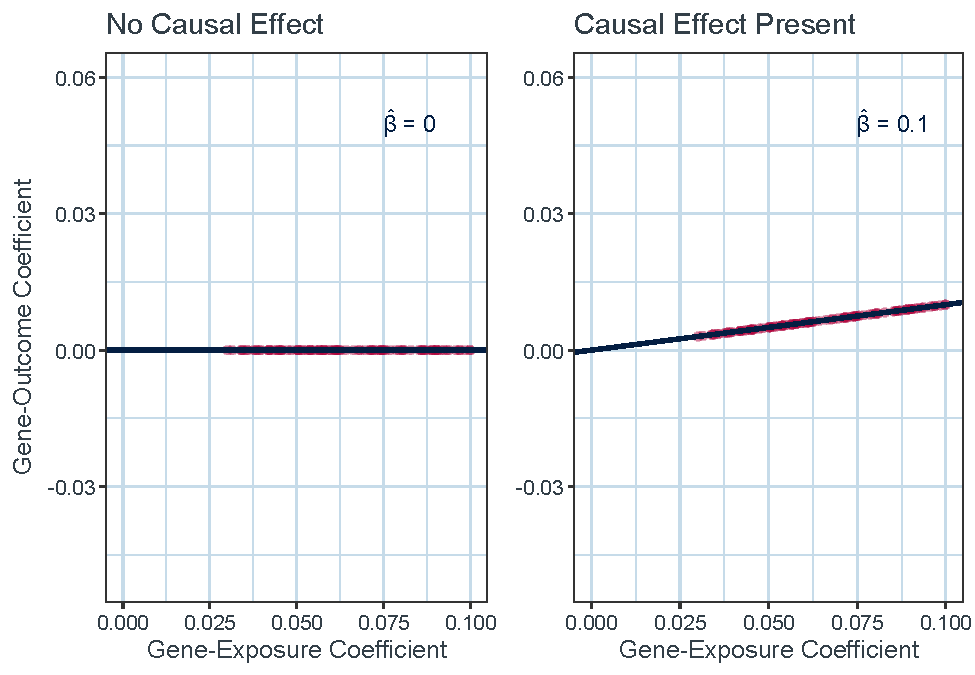
\includegraphics[keepaspectratio]{MSc_Thesis_Bookdown_files/figure-latex/test-plot-causal-1.pdf}}

\newpage

\subsubsection{Random Errors}\label{random-errors}

\leavevmode\newline Re-plotting the same graphs with non-zero random error terms (\texttt{rand\_error\ =\ TRUE}) should produce similar graphs with Gaussian spread around lines passing through the origin with gradients of 0 and 0.1 for no causal effect and causal effect, respectively:

\pandocbounded{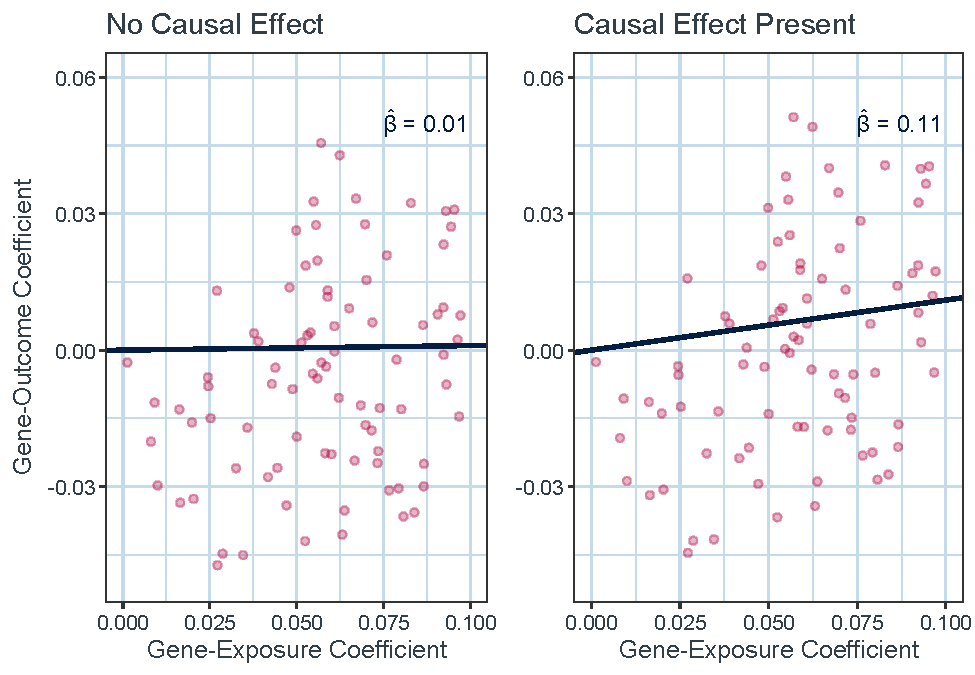
\includegraphics[keepaspectratio]{MSc_Thesis_Bookdown_files/figure-latex/test-plot-causal-errors-1.pdf}}

\newpage

\subsubsection{One versus Two Sample MR}\label{one-versus-two-sample-mr}

\leavevmode\newline Where gene-exposure coefficients and gene-outcome coefficients are estimated from two separate samples rather than one (i.e.~\texttt{two\_sample\ =\ TRUE}, simulating 2 sample MR), even with random error terms set to zero, error will be introduced into causal effect estimation through random sampling of different combinations of effect alleles. However, where a causal effect is not present, the effect estimated will consistently be zero regardless of the combinations of alleles sampled, so random error should not be introduced:

\pandocbounded{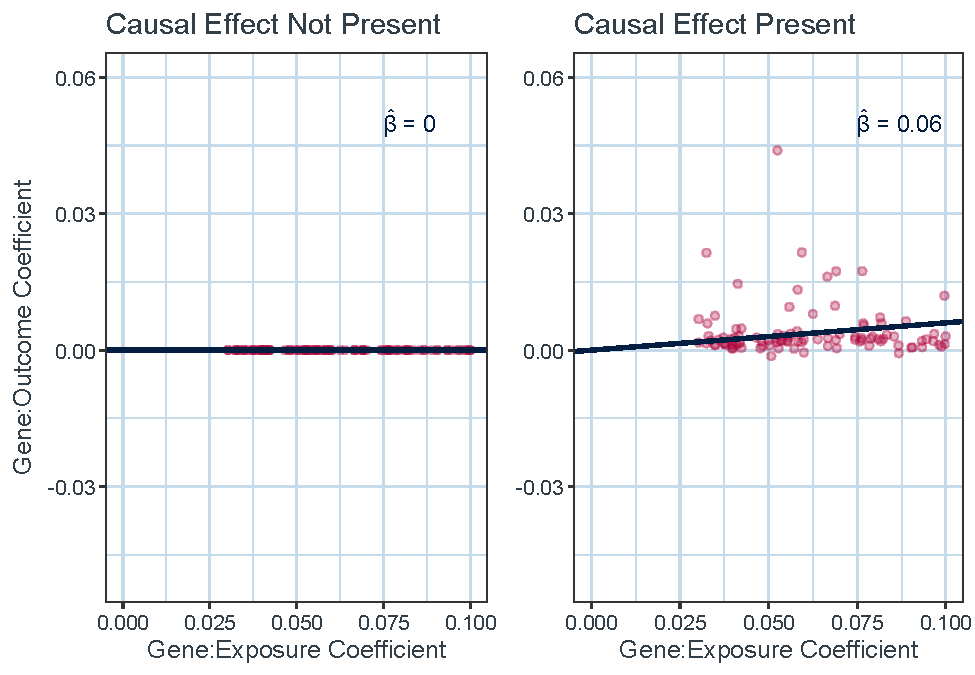
\includegraphics[keepaspectratio]{MSc_Thesis_Bookdown_files/figure-latex/test-plot-causal-2SMR-1.pdf}}

\newpage

\subsubsection{Invalid Instruments}\label{invalid-instruments}

\leavevmode\newline Where invalid instruments are present (i.e.~\texttt{prop\_invalid} \(\ne\) \texttt{0}) and random error terms are set to 0, graphs of gene-exposure coefficients versus gene-outcome coefficients should be straight lines through the origin and all points representing valid instruments; the invalid instruments should appear as outliers to this line:

\pandocbounded{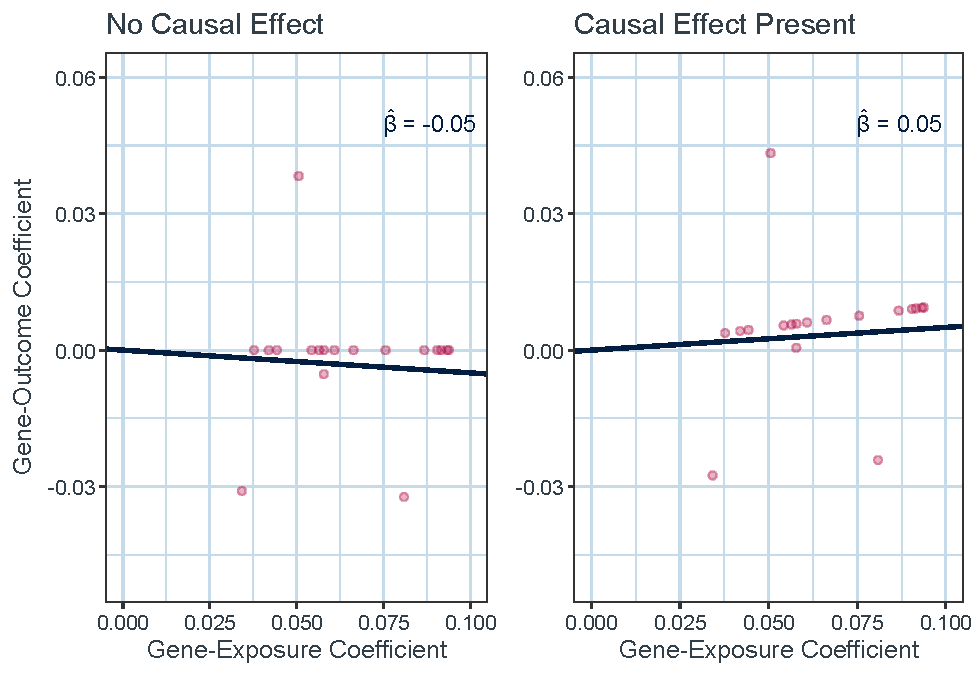
\includegraphics[keepaspectratio]{MSc_Thesis_Bookdown_files/figure-latex/test-plot-causal-inval-1.pdf}}

\newpage

\subsubsection{Balanced Versus Directional Pleiotropy}\label{balanced-versus-directional-pleiotropy}

\leavevmode\newline Replotting the above with unbalanced pleiotropy present (\texttt{balanced\_pleio\ =\ FALSE}), the invalid instruments should all appear as outliers in the positive direction, i.e.~steepening the line of best fit and leading to overestimation of the causal effect:

\pandocbounded{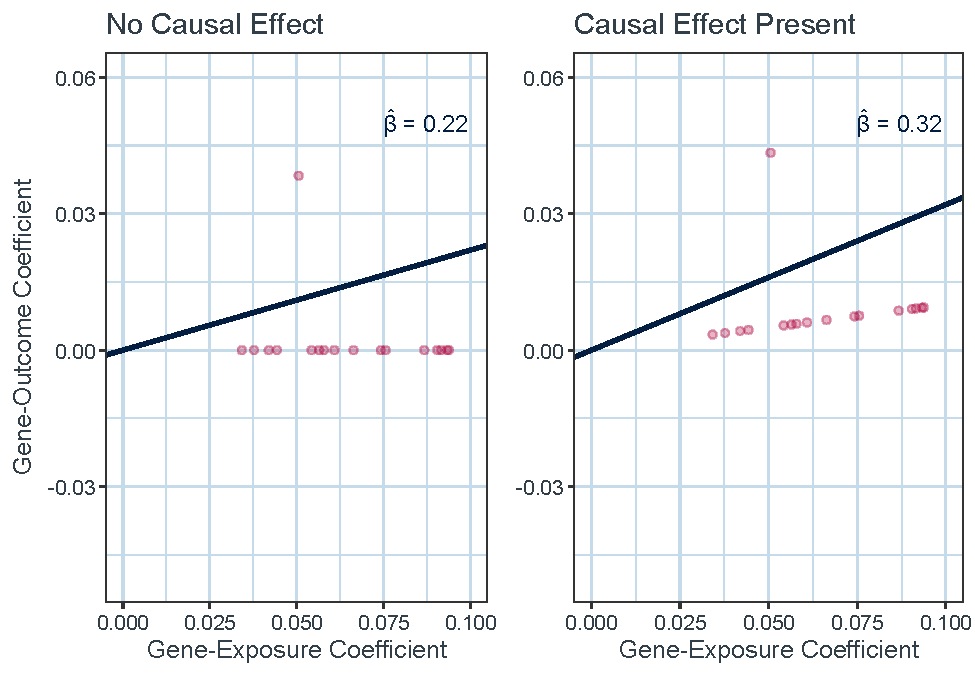
\includegraphics[keepaspectratio]{MSc_Thesis_Bookdown_files/figure-latex/test-plot-causal-unbal-1.pdf}}

\newpage

\subsubsection{InSIDE Assumption and Phi}\label{inside-assumption-and-phi}

\leavevmode\newline The variable phi represents additional pleiotropic effects of each invalid instrument when the \hyperref[acronyms_InSIDE]{InSIDE} assumption is not satisfied. The \hyperref[acronyms_InSIDE]{InSIDE} assumption states that the gene-exposure association is not correlated with the pleiotropic path gene-outcome path of any invalid genetic instruments. This assumption can be violated if e.g.:

\begin{itemize}
\item
  several invalid genetic instruments influence the outcome via the same pleiotropic path
\item
  several invalid genetic instruments are related to the same (unmeasured) confounders of the exposure:outcome relationship, aka correlated pleiotropy.
\end{itemize}

As such, when the \hyperref[acronyms_InSIDE]{InSIDE} assumption is violated, even ``strong'' instruments (i.e.~those with a strong gene-exposure relationship) may not allow accurate estimation of the true causal effect, as pleiotropic effects may scale with instrument strength. If pleiotropic effects are directional, \hyperref[acronyms_InSIDE]{InSIDE} assumption violation may lead to bias.

Bowden et al\textsuperscript{\citeproc{ref-bowden_consistent_2016}{8}} modeled phi as the pleiotropic effects of unmeasured genetic confounders of the exposure:outcome relationship. Phi adds additional error to causal effect estimation in scenarios with directional pleiotropic effects (\texttt{0\ \textless{}\ alpha\ \textless{}\ 0.2}) and \hyperref[acronyms_InSIDE]{InSIDE} assumption violation. As such, switching \texttt{InSIDE\_satisfied} from \texttt{TRUE} to \texttt{FALSE} should add scatter to the linear association expected when plotting alpha versus gene-outcome coefficients with random error terms set to zero:

\pandocbounded{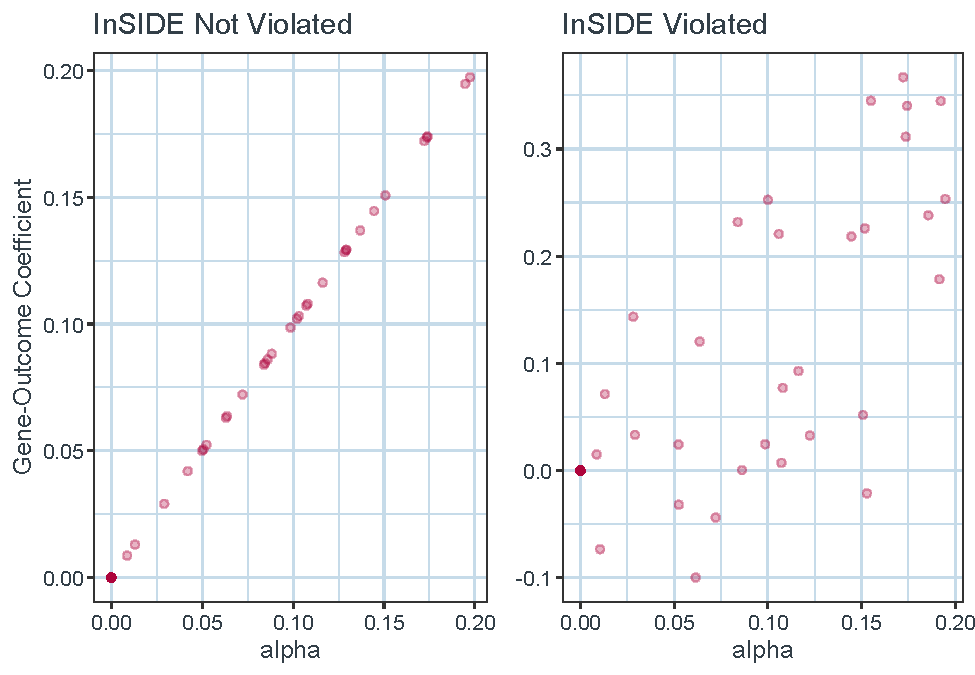
\includegraphics[keepaspectratio]{MSc_Thesis_Bookdown_files/figure-latex/test-plot-phi-1.pdf}}

\newpage

Setting \texttt{InSIDE\_satisfied\ =\ TRUE} should mean \texttt{phi\ =\ 0}; \texttt{InSIDE\_satisfied=FALSE} should result in \texttt{phi} \(\propto\) gene-outcome coefficient, with scatter only in the positive direction of gene-outcome coefficients given the simulation only uses the \texttt{phi} term in Scenario 3 (which requires directional pleiotropy):

\pandocbounded{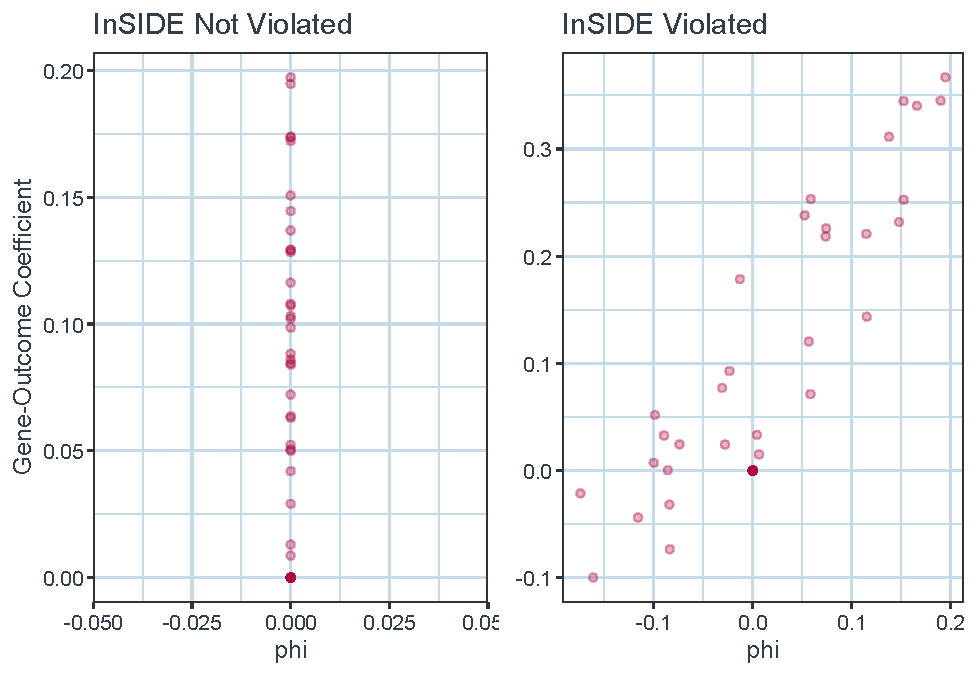
\includegraphics[keepaspectratio]{MSc_Thesis_Bookdown_files/figure-latex/test-plot-phi-2-1.pdf}}

\newpage

\subsection{Summary Table}\label{appendix-sim-summ}

A function (\texttt{get\_summary\_MR\_tib\_row}) was written to take models generated from each simulated dataset, estimate causal effect using both weighted median and MR-Hevo methodologies, then output a summary formatted as per Tables 2 \& 3 in Bowden et al\textsuperscript{\citeproc{ref-bowden_consistent_2016}{8}}:

\begin{Shaded}
\begin{Highlighting}[]
\CommentTok{\# Load WME functions}
\FunctionTok{library}\NormalTok{(TwoSampleMR)}

\CommentTok{\# Load RStan {-} needed for MR{-}Hevo}
\FunctionTok{library}\NormalTok{(rstan)}


\CommentTok{\# Run local copy of MR{-}Hevo functions}
\CommentTok{\# Not using full package due to conflicts with Windows}
\FunctionTok{source}\NormalTok{(here}\SpecialCharTok{::}\FunctionTok{here}\NormalTok{(}\StringTok{"Script"}\NormalTok{, }\StringTok{"Hevo"}\NormalTok{, }\StringTok{"functions.mrhevo.R"}\NormalTok{))}

\CommentTok{\# Standard set{-}up for RStan}
\FunctionTok{options}\NormalTok{(}\AttributeTok{mc.cores =}\NormalTok{ parallel}\SpecialCharTok{::}\FunctionTok{detectCores}\NormalTok{())}
\FunctionTok{rstan\_options}\NormalTok{(}\AttributeTok{auto\_write =} \ConstantTok{TRUE}\NormalTok{, }\AttributeTok{save\_dso =} \ConstantTok{TRUE}\NormalTok{)}


\CommentTok{\# Compile model for MR{-}Hevo}
\NormalTok{mr.stanmodel }\OtherTok{\textless{}{-}} \FunctionTok{stan\_model}\NormalTok{(}\AttributeTok{file=}\NormalTok{ here}\SpecialCharTok{::}\FunctionTok{here}\NormalTok{(}\StringTok{"Script"}\NormalTok{, }
                                            \StringTok{"Hevo"}\NormalTok{, }
                                            \StringTok{"MRHevo\_summarystats.stan"}\NormalTok{),}
                           \AttributeTok{model\_name=}\StringTok{"MRHevo.summarystats"}\NormalTok{, }
                           \AttributeTok{verbose=}\ConstantTok{FALSE}\NormalTok{,}
                           \AttributeTok{save\_dso =} \ConstantTok{TRUE}\NormalTok{,}
                           \AttributeTok{auto\_write =} \ConstantTok{TRUE}\NormalTok{)}

\NormalTok{get\_summary\_MR\_tib\_row }\OtherTok{\textless{}{-}} \ControlFlowTok{function}\NormalTok{(model\_list)\{}
  
  
  \CommentTok{\# Create output tibble in same format as Table 2/3 from}
  \CommentTok{\# Bowden et al}
\NormalTok{  output\_tib\_row }\OtherTok{\textless{}{-}} \FunctionTok{tibble}\NormalTok{(}\AttributeTok{N =} \FunctionTok{as.integer}\NormalTok{(),}
                           \AttributeTok{Prop\_Invalid =} \FunctionTok{as.double}\NormalTok{(),}
                           \AttributeTok{F\_stat =} \FunctionTok{as.double}\NormalTok{(),}
                           \AttributeTok{R2\_stat =} \FunctionTok{as.double}\NormalTok{(),}
                           \AttributeTok{WME\_Av =} \FunctionTok{as.double}\NormalTok{(),}
                           \AttributeTok{WME\_SE =} \FunctionTok{as.double}\NormalTok{(),}
                           \AttributeTok{WME\_Pos\_Rate =} \FunctionTok{as.double}\NormalTok{(),}
                           \AttributeTok{Hevo\_Av =} \FunctionTok{as.double}\NormalTok{(),}
                           \AttributeTok{Hevo\_SE =} \FunctionTok{as.double}\NormalTok{(),}
                           \AttributeTok{Hevo\_Pos\_Rate =} \FunctionTok{as.double}\NormalTok{())}
  
\NormalTok{  n\_datasets }\OtherTok{\textless{}{-}} \FunctionTok{length}\NormalTok{(model\_list)}
  
  \CommentTok{\# Create blank tibble to receive results of Weighted}
  \CommentTok{\# Median Estimator function from MR{-}Base}
  
\NormalTok{  results\_tib }\OtherTok{\textless{}{-}}  \FunctionTok{tibble}\NormalTok{(}\AttributeTok{WME\_est =} \FunctionTok{as.double}\NormalTok{(),}
                         \AttributeTok{WME\_se =} \FunctionTok{as.double}\NormalTok{(),}
                         \AttributeTok{WME\_pval =} \FunctionTok{as.double}\NormalTok{(),}
                         \AttributeTok{WME\_nsnp =} \FunctionTok{as.integer}\NormalTok{(),}
                         \AttributeTok{Hevo\_est =} \FunctionTok{as.double}\NormalTok{(),}
                         \AttributeTok{Hevo\_se =} \FunctionTok{as.double}\NormalTok{(),}
                         \AttributeTok{Hevo\_sd =} \FunctionTok{as.double}\NormalTok{(),}
                         \AttributeTok{Hevo\_est\_lower\_CI =} \FunctionTok{as.double}\NormalTok{(),}
                         \AttributeTok{Hevo\_est\_upper\_CI =} \FunctionTok{as.double}\NormalTok{(),}
                         \AttributeTok{Hevo\_causal\_detected =} \FunctionTok{as.logical}\NormalTok{()}
\NormalTok{  )}
  
  
  \CommentTok{\# Run WME and MR{-}Hevo for each dataset }
  \ControlFlowTok{for}\NormalTok{(dataset }\ControlFlowTok{in} \DecValTok{1}\SpecialCharTok{:}\NormalTok{n\_datasets)\{}
    
    \CommentTok{\# Stored as individual vectors for MR{-}Hevo/RStan {-} not}
    \CommentTok{\# Tidyverse compatible}
\NormalTok{    coeff\_G\_X\_vect }\OtherTok{\textless{}{-}}\NormalTok{ model\_list[[dataset]]}\SpecialCharTok{$}\NormalTok{coeff\_G\_X}
\NormalTok{    coeff\_G\_Y\_vect }\OtherTok{\textless{}{-}}\NormalTok{ model\_list[[dataset]]}\SpecialCharTok{$}\NormalTok{coeff\_G\_Y}
\NormalTok{    coeff\_G\_X\_SE\_vect }\OtherTok{\textless{}{-}}\NormalTok{ model\_list[[dataset]]}\SpecialCharTok{$}\NormalTok{coeff\_G\_X\_SE}
\NormalTok{    coeff\_G\_Y\_SE\_vect }\OtherTok{\textless{}{-}}\NormalTok{ model\_list[[dataset]]}\SpecialCharTok{$}\NormalTok{coeff\_G\_Y\_SE}
\NormalTok{    prop\_invalid }\OtherTok{\textless{}{-}} \FunctionTok{min}\NormalTok{(model\_list[[dataset]]}\SpecialCharTok{$}\NormalTok{prop\_invalid)}
\NormalTok{    F\_stat }\OtherTok{\textless{}{-}} \FunctionTok{min}\NormalTok{(model\_list[[dataset]]}\SpecialCharTok{$}\NormalTok{F\_stat)}
\NormalTok{    R2\_stat }\OtherTok{\textless{}{-}} \FunctionTok{min}\NormalTok{(model\_list[[dataset]]}\SpecialCharTok{$}\NormalTok{R2\_stat)}
\NormalTok{    n\_instruments }\OtherTok{\textless{}{-}} \FunctionTok{max}\NormalTok{(model\_list[[dataset]]}\SpecialCharTok{$}\NormalTok{Instrument)}
\NormalTok{    n\_participants }\OtherTok{\textless{}{-}} \FunctionTok{min}\NormalTok{(model\_list[[dataset]]}\SpecialCharTok{$}\NormalTok{n\_participants)}
    
    
    \CommentTok{\# N.B. MR{-}Hevo terminology vs WME paper/other code:}
    \CommentTok{\# alpha = effects of instruments on exposure, i.e. coeff\_G\_X}
    \CommentTok{\# beta = pleiotropic effects of instruments on outcome, i.e. alpha in WME}
    \CommentTok{\# gamma = effects of instruments on outcome, i.e. coeff\_G\_Y}
    \CommentTok{\# theta = causal effect X on Y, i.e. b}
    
    \CommentTok{\# Results from weighted median estimator method}
\NormalTok{    WME\_results }\OtherTok{\textless{}{-}} \FunctionTok{mr\_weighted\_median}\NormalTok{(}\AttributeTok{b\_exp =}\NormalTok{ coeff\_G\_X\_vect,}
                                      \AttributeTok{b\_out =}\NormalTok{ coeff\_G\_Y\_vect,}
                                      \AttributeTok{se\_exp =}\NormalTok{ coeff\_G\_X\_SE\_vect,}
                                      \AttributeTok{se\_out =}\NormalTok{ coeff\_G\_Y\_SE\_vect,}
                                      \AttributeTok{parameters =} \FunctionTok{list}\NormalTok{(}\AttributeTok{nboot =} \DecValTok{1000}\NormalTok{))}
    
    \CommentTok{\# Results from MR{-}Hevo method}
\NormalTok{    Hevo\_results}\OtherTok{\textless{}{-}} \FunctionTok{run\_mrhevo.sstats}\NormalTok{(}\AttributeTok{alpha\_hat =}\NormalTok{ coeff\_G\_X\_vect,}
                                     \AttributeTok{se.alpha\_hat =}\NormalTok{ coeff\_G\_X\_SE\_vect,}
                                     \AttributeTok{gamma\_hat =}\NormalTok{ coeff\_G\_Y\_vect,}
                                     \AttributeTok{se.gamma\_hat =}\NormalTok{ coeff\_G\_Y\_SE\_vect) }\SpecialCharTok{\%\textgreater{}\%}
      \FunctionTok{summary}\NormalTok{()}
    
    
    \CommentTok{\# Extract WME Results}
\NormalTok{    results\_tib[dataset, ]}\SpecialCharTok{$}\NormalTok{WME\_est }\OtherTok{\textless{}{-}}\NormalTok{ WME\_results}\SpecialCharTok{$}\NormalTok{b}
\NormalTok{    results\_tib[dataset, ]}\SpecialCharTok{$}\NormalTok{WME\_se }\OtherTok{\textless{}{-}}\NormalTok{ WME\_results}\SpecialCharTok{$}\NormalTok{se}
\NormalTok{    results\_tib[dataset, ]}\SpecialCharTok{$}\NormalTok{WME\_pval }\OtherTok{\textless{}{-}}\NormalTok{ WME\_results}\SpecialCharTok{$}\NormalTok{pval}
\NormalTok{    results\_tib[dataset, ]}\SpecialCharTok{$}\NormalTok{WME\_nsnp }\OtherTok{\textless{}{-}}\NormalTok{ WME\_results}\SpecialCharTok{$}\NormalTok{nsnp}
    
    \CommentTok{\# Extract MR{-}Hevo Results}
\NormalTok{    results\_tib[dataset, ]}\SpecialCharTok{$}\NormalTok{Hevo\_est }\OtherTok{\textless{}{-}}\NormalTok{ Hevo\_results}\SpecialCharTok{$}\NormalTok{summary[}\StringTok{"theta"}\NormalTok{,}\StringTok{"mean"}\NormalTok{]}
    \CommentTok{\# Below used in error {-} actually Monte Carlo SE}
\NormalTok{    results\_tib[dataset, ]}\SpecialCharTok{$}\NormalTok{Hevo\_se }\OtherTok{\textless{}{-}}\NormalTok{ Hevo\_results}\SpecialCharTok{$}\NormalTok{summary[}\StringTok{"theta"}\NormalTok{,}\StringTok{"se\_mean"}\NormalTok{] }
    \CommentTok{\# Below should have been used as SE {-} SD of bootstrap distribution}
\NormalTok{    results\_tib[dataset, ]}\SpecialCharTok{$}\NormalTok{Hevo\_sd }\OtherTok{\textless{}{-}}\NormalTok{ Hevo\_results}\SpecialCharTok{$}\NormalTok{summary[}\StringTok{"theta"}\NormalTok{,}\StringTok{"sd"}\NormalTok{] }
\NormalTok{    results\_tib[dataset, ]}\SpecialCharTok{$}\NormalTok{Hevo\_est\_lower\_CI }\OtherTok{\textless{}{-}}\NormalTok{ Hevo\_results}\SpecialCharTok{$}\NormalTok{summary[}\StringTok{"theta"}\NormalTok{,}\StringTok{"2.5\%"}\NormalTok{]}
\NormalTok{    results\_tib[dataset, ]}\SpecialCharTok{$}\NormalTok{Hevo\_est\_upper\_CI }\OtherTok{\textless{}{-}}\NormalTok{ Hevo\_results}\SpecialCharTok{$}\NormalTok{summary[}\StringTok{"theta"}\NormalTok{,}\StringTok{"97.5\%"}\NormalTok{]}
    
\NormalTok{  \}}
  
  \CommentTok{\# Add causality Boolean to MR{-}Hevo}
\NormalTok{  results\_tib }\OtherTok{\textless{}{-}}\NormalTok{ results\_tib }\SpecialCharTok{\%\textgreater{}\%}
    \FunctionTok{mutate}\NormalTok{(}\AttributeTok{Hevo\_est\_causal\_detected =}\NormalTok{ (Hevo\_est\_lower\_CI }\SpecialCharTok{\textgreater{}} \DecValTok{0}  \SpecialCharTok{|}\NormalTok{ Hevo\_est\_upper\_CI }\SpecialCharTok{\textless{}} \DecValTok{0}\NormalTok{))}
  
  
\NormalTok{  output\_tib\_row }\OtherTok{\textless{}{-}}\NormalTok{ results\_tib }\SpecialCharTok{\%\textgreater{}\%} 
    \FunctionTok{summarise}\NormalTok{(}\AttributeTok{N =}\NormalTok{ n\_participants,}
              \AttributeTok{Prop\_Invalid =}\NormalTok{ prop\_invalid,}
              \AttributeTok{F\_stat =} \FunctionTok{mean}\NormalTok{(F\_stat),}
              \AttributeTok{R2\_stat =} \FunctionTok{mean}\NormalTok{(R2\_stat),}
              \AttributeTok{WME\_Av =} \FunctionTok{mean}\NormalTok{(WME\_est),}
              \AttributeTok{WME\_SE =} \FunctionTok{mean}\NormalTok{(WME\_se),}
              \AttributeTok{WME\_Pos\_Rate =} \FunctionTok{length}\NormalTok{(WME\_pval[WME\_pval }\SpecialCharTok{\textless{}} \FloatTok{0.05}\NormalTok{]) }\SpecialCharTok{/}\NormalTok{ n\_datasets,}
              \AttributeTok{Hevo\_Av =} \FunctionTok{mean}\NormalTok{(Hevo\_est),}
              \AttributeTok{Hevo\_SE =} \FunctionTok{mean}\NormalTok{(Hevo\_se),}
              \AttributeTok{Hevo\_Lower\_CI =} \FunctionTok{mean}\NormalTok{(Hevo\_est\_lower\_CI),}
              \AttributeTok{Hevo\_Upper\_CI =} \FunctionTok{mean}\NormalTok{(Hevo\_est\_upper\_CI),}
              \AttributeTok{Hevo\_Pos\_Rate =} \FunctionTok{sum}\NormalTok{(Hevo\_est\_causal\_detected) }\SpecialCharTok{/}\NormalTok{ n\_datasets}
\NormalTok{    ) }\SpecialCharTok{\%\textgreater{}\%} 
    \FunctionTok{mutate}\NormalTok{(}\FunctionTok{across}\NormalTok{(where}\SpecialCharTok{::}\FunctionTok{here}\NormalTok{(is.double), round, }\DecValTok{3}\NormalTok{))}
  
  \FunctionTok{return}\NormalTok{(output\_tib\_row)}
  
\NormalTok{\}}
\end{Highlighting}
\end{Shaded}

\begin{Shaded}
\begin{Highlighting}[]
\NormalTok{test\_tib\_summ\_MR\_data }\OtherTok{\textless{}{-}}  \FunctionTok{get\_simulated\_MR\_data}\NormalTok{(}\AttributeTok{n\_participants =} \DecValTok{10000}\NormalTok{,}
                                                \AttributeTok{n\_instruments =} \DecValTok{25}\NormalTok{,}
                                                \AttributeTok{n\_datasets =} \DecValTok{2}\NormalTok{,}
                                                \AttributeTok{prop\_invalid =} \FloatTok{0.1}\NormalTok{,}
                                                \AttributeTok{beta\_val =} \FloatTok{0.1}\NormalTok{,}
                                                \AttributeTok{causal\_effect =} \ConstantTok{TRUE}\NormalTok{,}
                                                \AttributeTok{rand\_error =} \ConstantTok{TRUE}\NormalTok{,}
                                                \AttributeTok{two\_sample =} \ConstantTok{TRUE}\NormalTok{,}
                                                \AttributeTok{balanced\_pleio =} \ConstantTok{TRUE}\NormalTok{,}
                                                \AttributeTok{InSIDE\_satisfied =} \ConstantTok{TRUE}\NormalTok{)}

\NormalTok{test\_tib\_summ\_MR\_models }\OtherTok{\textless{}{-}} \FunctionTok{get\_models}\NormalTok{(test\_tib\_summ\_MR\_data)}

\NormalTok{test\_tib\_summ\_MR\_row }\OtherTok{\textless{}{-}} \FunctionTok{get\_summary\_MR\_tib\_row}\NormalTok{(test\_tib\_summ\_MR\_models)}
\end{Highlighting}
\end{Shaded}

\begin{verbatim}
## 
## CHECKING DATA AND PREPROCESSING FOR MODEL 'MRHevo.summarystats' NOW.
## 
## COMPILING MODEL 'MRHevo.summarystats' NOW.
## 
## STARTING SAMPLER FOR MODEL 'MRHevo.summarystats' NOW.
\end{verbatim}

\begin{verbatim}
## 
## CHECKING DATA AND PREPROCESSING FOR MODEL 'MRHevo.summarystats' NOW.
## 
## COMPILING MODEL 'MRHevo.summarystats' NOW.
## 
## STARTING SAMPLER FOR MODEL 'MRHevo.summarystats' NOW.
\end{verbatim}

\begin{Shaded}
\begin{Highlighting}[]
\NormalTok{test\_tib\_summ\_MR\_row }\SpecialCharTok{\%\textgreater{}\%} 
  \FunctionTok{kable}\NormalTok{() }\SpecialCharTok{\%\textgreater{}\%} 
  \FunctionTok{kable\_styling}\NormalTok{(}\AttributeTok{latex\_options=}\StringTok{"scale\_down"}\NormalTok{)}
\end{Highlighting}
\end{Shaded}

\begin{table}
\centering
\resizebox{\ifdim\width>\linewidth\linewidth\else\width\fi}{!}{
\begin{tabular}{r|r|r|r|r|r|r|r|r|r|r|r}
\hline
N & Prop\_Invalid & F\_stat & R2\_stat & WME\_Av & WME\_SE & WME\_Pos\_Rate & Hevo\_Av & Hevo\_SE & Hevo\_Lower\_CI & Hevo\_Upper\_CI & Hevo\_Pos\_Rate\\
\hline
10000 & 0.1 & 14.739 & 0.036 & 0.091 & 0.09 & 0.5 & 0.121 & 0.001 & -0.052 & 0.302 & 0\\
\hline
\end{tabular}}
\end{table}

\newpage

\section{Appendix: Sensitivity Analyses}\label{appendix-sens}

\subsection{Simulation Study (Post-Hoc)}\label{appendix-sens-post-hoc}

\subsubsection{100 Genetic Instruments}\label{sens-tibs-100-snp}

\global\setlength{\Oldarrayrulewidth}{\arrayrulewidth}

\global\setlength{\Oldtabcolsep}{\tabcolsep}

\setlength{\tabcolsep}{2pt}

\renewcommand*{\arraystretch}{1.3}



\providecommand{\ascline}[3]{\noalign{\global\arrayrulewidth #1}\arrayrulecolor[HTML]{#2}\cline{#3}}

\begin{longtable}[c]{|p{0.44in}|p{0.57in}|p{0.35in}|p{0.42in}|p{0.51in}|p{0.45in}|p{0.65in}|p{0.44in}|p{0.19in}|p{0.51in}|p{0.45in}|p{0.65in}|p{0.44in}}

\caption{Summary\ of\ 100\ simulated\ Mendelian\ randomisation\ studies\ per\ combination\ of\ scenario\ and\ parameters,\ all\ with\ null\ causal\ effect\ and\ using\ 20,000\ participants\ with\ 100\ genetic\ instruments}\label{tab:sens-100-snp-no-causal-sim-summ-display}\\

\ascline{1.5pt}{666666}{1-13}

\multicolumn{1}{>{\centering}m{\dimexpr 0.44in+0\tabcolsep}}{} & \multicolumn{1}{>{\centering}m{\dimexpr 0.57in+0\tabcolsep}}{} & \multicolumn{1}{>{\centering}m{\dimexpr 0.35in+0\tabcolsep}}{} & \multicolumn{1}{>{\centering}m{\dimexpr 0.42in+0\tabcolsep}}{} & \multicolumn{4}{>{\centering}m{\dimexpr 2.06in+6\tabcolsep}}{\textcolor[HTML]{000000}{\fontsize{9}{9}\selectfont{\global\setmainfont{Arial}{Weighted}}}} & \multicolumn{1}{>{\centering}m{\dimexpr 0.19in+0\tabcolsep}}{\textcolor[HTML]{000000}{\fontsize{9}{9}\selectfont{\global\setmainfont{Arial}{}}}} & \multicolumn{4}{>{\centering}m{\dimexpr 2.06in+6\tabcolsep}}{\textcolor[HTML]{000000}{\fontsize{9}{9}\selectfont{\global\setmainfont{Arial}{MR}}}} \\





\multicolumn{1}{>{\centering}m{\dimexpr 0.44in+0\tabcolsep}}{} & \multicolumn{1}{>{\centering}m{\dimexpr 0.57in+0\tabcolsep}}{} & \multicolumn{1}{>{\centering}m{\dimexpr 0.35in+0\tabcolsep}}{} & \multicolumn{1}{>{\centering}m{\dimexpr 0.42in+0\tabcolsep}}{} & \multicolumn{4}{>{\centering}m{\dimexpr 2.06in+6\tabcolsep}}{\textcolor[HTML]{000000}{\fontsize{9}{9}\selectfont{\global\setmainfont{Arial}{Median}}}} & \multicolumn{1}{>{\centering}m{\dimexpr 0.19in+0\tabcolsep}}{\textcolor[HTML]{000000}{\fontsize{9}{9}\selectfont{\global\setmainfont{Arial}{}}}} & \multicolumn{4}{>{\centering}m{\dimexpr 2.06in+6\tabcolsep}}{\textcolor[HTML]{000000}{\fontsize{9}{9}\selectfont{\global\setmainfont{Arial}{Hevo}}}} \\

\ascline{1pt}{000000}{5-8}\ascline{1pt}{000000}{10-13}



\multicolumn{1}{>{\centering}m{\dimexpr 0.44in+0\tabcolsep}}{} & \multicolumn{1}{>{\centering}m{\dimexpr 0.57in+0\tabcolsep}}{} & \multicolumn{1}{>{\centering}m{\dimexpr 0.35in+0\tabcolsep}}{} & \multicolumn{1}{>{\centering}m{\dimexpr 0.42in+0\tabcolsep}}{} & \multicolumn{2}{>{\centering}m{\dimexpr 0.96in+2\tabcolsep}}{\textcolor[HTML]{000000}{\fontsize{9}{9}\selectfont{\global\setmainfont{Arial}{Mean\ Estimate}}}} & \multicolumn{1}{>{\centering}m{\dimexpr 0.65in+0\tabcolsep}}{\textcolor[HTML]{000000}{\fontsize{9}{9}\selectfont{\global\setmainfont{Arial}{Mean}}}} & \multicolumn{1}{>{\centering}m{\dimexpr 0.44in+0\tabcolsep}}{\textcolor[HTML]{000000}{\fontsize{9}{9}\selectfont{\global\setmainfont{Arial}{Causal}}}} & \multicolumn{1}{>{\centering}m{\dimexpr 0.19in+0\tabcolsep}}{\textcolor[HTML]{000000}{\fontsize{9}{9}\selectfont{\global\setmainfont{Arial}{}}}} & \multicolumn{2}{>{\centering}m{\dimexpr 0.96in+2\tabcolsep}}{\textcolor[HTML]{000000}{\fontsize{9}{9}\selectfont{\global\setmainfont{Arial}{Mean\ Estimate}}}} & \multicolumn{1}{>{\centering}m{\dimexpr 0.65in+0\tabcolsep}}{\textcolor[HTML]{000000}{\fontsize{9}{9}\selectfont{\global\setmainfont{Arial}{Mean}}}} & \multicolumn{1}{>{\centering}m{\dimexpr 0.44in+0\tabcolsep}}{\textcolor[HTML]{000000}{\fontsize{9}{9}\selectfont{\global\setmainfont{Arial}{Causal}}}} \\





\multicolumn{1}{>{\centering}m{\dimexpr 0.44in+0\tabcolsep}}{} & \multicolumn{1}{>{\centering}m{\dimexpr 0.57in+0\tabcolsep}}{} & \multicolumn{1}{>{\centering}m{\dimexpr 0.35in+0\tabcolsep}}{} & \multicolumn{1}{>{\centering}m{\dimexpr 0.42in+0\tabcolsep}}{} & \multicolumn{1}{>{\centering}m{\dimexpr 0.51in+0\tabcolsep}}{} & \multicolumn{1}{>{\centering}m{\dimexpr 0.45in+0\tabcolsep}}{} & \multicolumn{1}{>{\centering}m{\dimexpr 0.65in+0\tabcolsep}}{} & \multicolumn{1}{>{\centering}m{\dimexpr 0.44in+0\tabcolsep}}{\textcolor[HTML]{000000}{\fontsize{9}{9}\selectfont{\global\setmainfont{Arial}{Report}}}} & \multicolumn{1}{>{\centering}m{\dimexpr 0.19in+0\tabcolsep}}{\textcolor[HTML]{000000}{\fontsize{9}{9}\selectfont{\global\setmainfont{Arial}{}}}} & \multicolumn{1}{>{\centering}m{\dimexpr 0.51in+0\tabcolsep}}{} & \multicolumn{1}{>{\centering}m{\dimexpr 0.45in+0\tabcolsep}}{} & \multicolumn{1}{>{\centering}m{\dimexpr 0.65in+0\tabcolsep}}{} & \multicolumn{1}{>{\centering}m{\dimexpr 0.44in+0\tabcolsep}}{\textcolor[HTML]{000000}{\fontsize{9}{9}\selectfont{\global\setmainfont{Arial}{Report}}}} \\





\multicolumn{1}{>{\centering}m{\dimexpr 0.44in+0\tabcolsep}}{\multirow[c]{-5}{*}{\parbox{0.44in}{\centering \textcolor[HTML]{000000}{\fontsize{9}{9}\selectfont{\global\setmainfont{Arial}{\textit{N}}}}}}} & \multicolumn{1}{>{\centering}m{\dimexpr 0.57in+0\tabcolsep}}{\multirow[c]{-5}{*}{\parbox{0.57in}{\centering \textcolor[HTML]{000000}{\fontsize{9}{9}\selectfont{\global\setmainfont{Arial}{Invalid\ IVs}}}}}} & \multicolumn{1}{>{\centering}m{\dimexpr 0.35in+0\tabcolsep}}{\multirow[c]{-5}{*}{\parbox{0.35in}{\centering \textcolor[HTML]{000000}{\fontsize{9}{9}\selectfont{\global\setmainfont{Arial}{\textit{F}}}}}}} & \multicolumn{1}{>{\centering}m{\dimexpr 0.42in+0\tabcolsep}}{\multirow[c]{-5}{*}{\parbox{0.42in}{\centering \textcolor[HTML]{000000}{\fontsize{9}{9}\selectfont{\global\setmainfont{Arial}{\textit{R}}}}\textcolor[HTML]{000000}{\fontsize{9}{9}\selectfont{\global\setmainfont{Arial}{\textit{\textsuperscript{2}}}}}}}} & \multicolumn{2}{>{\centering}m{\dimexpr 0.96in+2\tabcolsep}}{\multirow[c]{-2}{*}{\parbox{0.51in}{\centering \textcolor[HTML]{000000}{\fontsize{9}{9}\selectfont{\global\setmainfont{Arial}{(Mean\ SE)}}}}}} & \multicolumn{1}{>{\centering}m{\dimexpr 0.65in+0\tabcolsep}}{\multirow[c]{-2}{*}{\parbox{0.65in}{\centering \textcolor[HTML]{000000}{\fontsize{9}{9}\selectfont{\global\setmainfont{Arial}{95\%\ CI}}}}}} & \multicolumn{1}{>{\centering}m{\dimexpr 0.44in+0\tabcolsep}}{\textcolor[HTML]{000000}{\fontsize{9}{9}\selectfont{\global\setmainfont{Arial}{Rate}}}} & \multicolumn{1}{>{\centering}m{\dimexpr 0.19in+0\tabcolsep}}{\textcolor[HTML]{000000}{\fontsize{9}{9}\selectfont{\global\setmainfont{Arial}{}}}} & \multicolumn{2}{>{\centering}m{\dimexpr 0.96in+2\tabcolsep}}{\multirow[c]{-2}{*}{\parbox{0.51in}{\centering \textcolor[HTML]{000000}{\fontsize{9}{9}\selectfont{\global\setmainfont{Arial}{(Mean\ SE*)}}}}}} & \multicolumn{1}{>{\centering}m{\dimexpr 0.65in+0\tabcolsep}}{\multirow[c]{-2}{*}{\parbox{0.65in}{\centering \textcolor[HTML]{000000}{\fontsize{9}{9}\selectfont{\global\setmainfont{Arial}{95\%\ CI}}}}}} & \multicolumn{1}{>{\centering}m{\dimexpr 0.44in+0\tabcolsep}}{\textcolor[HTML]{000000}{\fontsize{9}{9}\selectfont{\global\setmainfont{Arial}{Rate}}}} \\

\ascline{1.5pt}{666666}{1-13}\endfirsthead \caption[]{Summary\ of\ 100\ simulated\ Mendelian\ randomisation\ studies\ per\ combination\ of\ scenario\ and\ parameters,\ all\ with\ null\ causal\ effect\ and\ using\ 20,000\ participants\ with\ 100\ genetic\ instruments}\label{tab:sens-100-snp-no-causal-sim-summ-display}\\

\ascline{1.5pt}{666666}{1-13}

\multicolumn{1}{>{\centering}m{\dimexpr 0.44in+0\tabcolsep}}{} & \multicolumn{1}{>{\centering}m{\dimexpr 0.57in+0\tabcolsep}}{} & \multicolumn{1}{>{\centering}m{\dimexpr 0.35in+0\tabcolsep}}{} & \multicolumn{1}{>{\centering}m{\dimexpr 0.42in+0\tabcolsep}}{} & \multicolumn{4}{>{\centering}m{\dimexpr 2.06in+6\tabcolsep}}{\textcolor[HTML]{000000}{\fontsize{9}{9}\selectfont{\global\setmainfont{Arial}{Weighted}}}} & \multicolumn{1}{>{\centering}m{\dimexpr 0.19in+0\tabcolsep}}{\textcolor[HTML]{000000}{\fontsize{9}{9}\selectfont{\global\setmainfont{Arial}{}}}} & \multicolumn{4}{>{\centering}m{\dimexpr 2.06in+6\tabcolsep}}{\textcolor[HTML]{000000}{\fontsize{9}{9}\selectfont{\global\setmainfont{Arial}{MR}}}} \\





\multicolumn{1}{>{\centering}m{\dimexpr 0.44in+0\tabcolsep}}{} & \multicolumn{1}{>{\centering}m{\dimexpr 0.57in+0\tabcolsep}}{} & \multicolumn{1}{>{\centering}m{\dimexpr 0.35in+0\tabcolsep}}{} & \multicolumn{1}{>{\centering}m{\dimexpr 0.42in+0\tabcolsep}}{} & \multicolumn{4}{>{\centering}m{\dimexpr 2.06in+6\tabcolsep}}{\textcolor[HTML]{000000}{\fontsize{9}{9}\selectfont{\global\setmainfont{Arial}{Median}}}} & \multicolumn{1}{>{\centering}m{\dimexpr 0.19in+0\tabcolsep}}{\textcolor[HTML]{000000}{\fontsize{9}{9}\selectfont{\global\setmainfont{Arial}{}}}} & \multicolumn{4}{>{\centering}m{\dimexpr 2.06in+6\tabcolsep}}{\textcolor[HTML]{000000}{\fontsize{9}{9}\selectfont{\global\setmainfont{Arial}{Hevo}}}} \\

\ascline{1pt}{000000}{5-8}\ascline{1pt}{000000}{10-13}



\multicolumn{1}{>{\centering}m{\dimexpr 0.44in+0\tabcolsep}}{} & \multicolumn{1}{>{\centering}m{\dimexpr 0.57in+0\tabcolsep}}{} & \multicolumn{1}{>{\centering}m{\dimexpr 0.35in+0\tabcolsep}}{} & \multicolumn{1}{>{\centering}m{\dimexpr 0.42in+0\tabcolsep}}{} & \multicolumn{2}{>{\centering}m{\dimexpr 0.96in+2\tabcolsep}}{\textcolor[HTML]{000000}{\fontsize{9}{9}\selectfont{\global\setmainfont{Arial}{Mean\ Estimate}}}} & \multicolumn{1}{>{\centering}m{\dimexpr 0.65in+0\tabcolsep}}{\textcolor[HTML]{000000}{\fontsize{9}{9}\selectfont{\global\setmainfont{Arial}{Mean}}}} & \multicolumn{1}{>{\centering}m{\dimexpr 0.44in+0\tabcolsep}}{\textcolor[HTML]{000000}{\fontsize{9}{9}\selectfont{\global\setmainfont{Arial}{Causal}}}} & \multicolumn{1}{>{\centering}m{\dimexpr 0.19in+0\tabcolsep}}{\textcolor[HTML]{000000}{\fontsize{9}{9}\selectfont{\global\setmainfont{Arial}{}}}} & \multicolumn{2}{>{\centering}m{\dimexpr 0.96in+2\tabcolsep}}{\textcolor[HTML]{000000}{\fontsize{9}{9}\selectfont{\global\setmainfont{Arial}{Mean\ Estimate}}}} & \multicolumn{1}{>{\centering}m{\dimexpr 0.65in+0\tabcolsep}}{\textcolor[HTML]{000000}{\fontsize{9}{9}\selectfont{\global\setmainfont{Arial}{Mean}}}} & \multicolumn{1}{>{\centering}m{\dimexpr 0.44in+0\tabcolsep}}{\textcolor[HTML]{000000}{\fontsize{9}{9}\selectfont{\global\setmainfont{Arial}{Causal}}}} \\





\multicolumn{1}{>{\centering}m{\dimexpr 0.44in+0\tabcolsep}}{} & \multicolumn{1}{>{\centering}m{\dimexpr 0.57in+0\tabcolsep}}{} & \multicolumn{1}{>{\centering}m{\dimexpr 0.35in+0\tabcolsep}}{} & \multicolumn{1}{>{\centering}m{\dimexpr 0.42in+0\tabcolsep}}{} & \multicolumn{1}{>{\centering}m{\dimexpr 0.51in+0\tabcolsep}}{} & \multicolumn{1}{>{\centering}m{\dimexpr 0.45in+0\tabcolsep}}{} & \multicolumn{1}{>{\centering}m{\dimexpr 0.65in+0\tabcolsep}}{} & \multicolumn{1}{>{\centering}m{\dimexpr 0.44in+0\tabcolsep}}{\textcolor[HTML]{000000}{\fontsize{9}{9}\selectfont{\global\setmainfont{Arial}{Report}}}} & \multicolumn{1}{>{\centering}m{\dimexpr 0.19in+0\tabcolsep}}{\textcolor[HTML]{000000}{\fontsize{9}{9}\selectfont{\global\setmainfont{Arial}{}}}} & \multicolumn{1}{>{\centering}m{\dimexpr 0.51in+0\tabcolsep}}{} & \multicolumn{1}{>{\centering}m{\dimexpr 0.45in+0\tabcolsep}}{} & \multicolumn{1}{>{\centering}m{\dimexpr 0.65in+0\tabcolsep}}{} & \multicolumn{1}{>{\centering}m{\dimexpr 0.44in+0\tabcolsep}}{\textcolor[HTML]{000000}{\fontsize{9}{9}\selectfont{\global\setmainfont{Arial}{Report}}}} \\





\multicolumn{1}{>{\centering}m{\dimexpr 0.44in+0\tabcolsep}}{\multirow[c]{-5}{*}{\parbox{0.44in}{\centering \textcolor[HTML]{000000}{\fontsize{9}{9}\selectfont{\global\setmainfont{Arial}{\textit{N}}}}}}} & \multicolumn{1}{>{\centering}m{\dimexpr 0.57in+0\tabcolsep}}{\multirow[c]{-5}{*}{\parbox{0.57in}{\centering \textcolor[HTML]{000000}{\fontsize{9}{9}\selectfont{\global\setmainfont{Arial}{Invalid\ IVs}}}}}} & \multicolumn{1}{>{\centering}m{\dimexpr 0.35in+0\tabcolsep}}{\multirow[c]{-5}{*}{\parbox{0.35in}{\centering \textcolor[HTML]{000000}{\fontsize{9}{9}\selectfont{\global\setmainfont{Arial}{\textit{F}}}}}}} & \multicolumn{1}{>{\centering}m{\dimexpr 0.42in+0\tabcolsep}}{\multirow[c]{-5}{*}{\parbox{0.42in}{\centering \textcolor[HTML]{000000}{\fontsize{9}{9}\selectfont{\global\setmainfont{Arial}{\textit{R}}}}\textcolor[HTML]{000000}{\fontsize{9}{9}\selectfont{\global\setmainfont{Arial}{\textit{\textsuperscript{2}}}}}}}} & \multicolumn{2}{>{\centering}m{\dimexpr 0.96in+2\tabcolsep}}{\multirow[c]{-2}{*}{\parbox{0.51in}{\centering \textcolor[HTML]{000000}{\fontsize{9}{9}\selectfont{\global\setmainfont{Arial}{(Mean\ SE)}}}}}} & \multicolumn{1}{>{\centering}m{\dimexpr 0.65in+0\tabcolsep}}{\multirow[c]{-2}{*}{\parbox{0.65in}{\centering \textcolor[HTML]{000000}{\fontsize{9}{9}\selectfont{\global\setmainfont{Arial}{95\%\ CI}}}}}} & \multicolumn{1}{>{\centering}m{\dimexpr 0.44in+0\tabcolsep}}{\textcolor[HTML]{000000}{\fontsize{9}{9}\selectfont{\global\setmainfont{Arial}{Rate}}}} & \multicolumn{1}{>{\centering}m{\dimexpr 0.19in+0\tabcolsep}}{\textcolor[HTML]{000000}{\fontsize{9}{9}\selectfont{\global\setmainfont{Arial}{}}}} & \multicolumn{2}{>{\centering}m{\dimexpr 0.96in+2\tabcolsep}}{\multirow[c]{-2}{*}{\parbox{0.51in}{\centering \textcolor[HTML]{000000}{\fontsize{9}{9}\selectfont{\global\setmainfont{Arial}{(Mean\ SE*)}}}}}} & \multicolumn{1}{>{\centering}m{\dimexpr 0.65in+0\tabcolsep}}{\multirow[c]{-2}{*}{\parbox{0.65in}{\centering \textcolor[HTML]{000000}{\fontsize{9}{9}\selectfont{\global\setmainfont{Arial}{95\%\ CI}}}}}} & \multicolumn{1}{>{\centering}m{\dimexpr 0.44in+0\tabcolsep}}{\textcolor[HTML]{000000}{\fontsize{9}{9}\selectfont{\global\setmainfont{Arial}{Rate}}}} \\

\ascline{1.5pt}{666666}{1-13}\endhead



\multicolumn{13}{>{\raggedright}m{\dimexpr 6.08in+24\tabcolsep}}{\textcolor[HTML]{000000}{\fontsize{8}{8}\selectfont{\global\setmainfont{Arial}{CI:\ Confidence\ Interval,\ InSIDE:\ Instrument\ Strength\ Independent\ of\ Direct\ Effect,\ IV:\ Instumental\ Variable,\ SE:\ Standard\ Error,\ SE*:\ Estimated\ Standard\ Error.\ F\ and\ R²\ statistics\ presented\ are\ the\ minimum\ values\ across\ all\ simulated\ datasets.\ }}}\textcolor[HTML]{000000}{\fontsize{8}{8}\selectfont{\global\setmainfont{Arial}{\linebreak }}}\textcolor[HTML]{000000}{\fontsize{8}{8}\selectfont{\global\setmainfont{Arial}{Null\ Causal\ Effect\ (β\ =\ 0)}}}} \\

\endlastfoot



\multicolumn{13}{>{\centering}m{\dimexpr 6.08in+24\tabcolsep}}{\textcolor[HTML]{000000}{\fontsize{8}{8}\selectfont{\global\setmainfont{Arial}{Scenario\ 1:\ Balanced\ pleiotropy,\ InSIDE\ assumption\ satisfied}}}} \\





\multicolumn{1}{>{\centering}m{\dimexpr 0.44in+0\tabcolsep}}{\textcolor[HTML]{000000}{\fontsize{8}{8}\selectfont{\global\setmainfont{Arial}{20,000}}}} & \multicolumn{1}{>{\centering}m{\dimexpr 0.57in+0\tabcolsep}}{\textcolor[HTML]{000000}{\fontsize{8}{8}\selectfont{\global\setmainfont{Arial}{0\%}}}} & \multicolumn{1}{>{\centering}m{\dimexpr 0.35in+0\tabcolsep}}{\textcolor[HTML]{000000}{\fontsize{8}{8}\selectfont{\global\setmainfont{Arial}{24.1}}}} & \multicolumn{1}{>{\centering}m{\dimexpr 0.42in+0\tabcolsep}}{\textcolor[HTML]{000000}{\fontsize{8}{8}\selectfont{\global\setmainfont{Arial}{10.8\%}}}} & \multicolumn{1}{>{\raggedleft}m{\dimexpr 0.51in+0\tabcolsep}}{\textcolor[HTML]{000000}{\fontsize{8}{8}\selectfont{\global\setmainfont{Arial}{-0.003}}}} & \multicolumn{1}{>{\raggedright}m{\dimexpr 0.45in+0\tabcolsep}}{\textcolor[HTML]{000000}{\fontsize{8}{8}\selectfont{\global\setmainfont{Arial}{(0.031)}}}} & \multicolumn{1}{>{\centering}m{\dimexpr 0.65in+0\tabcolsep}}{\textcolor[HTML]{000000}{\fontsize{8}{8}\selectfont{\global\setmainfont{Arial}{-0.06\ to\ 0.06}}}} & \multicolumn{1}{>{\centering}m{\dimexpr 0.44in+0\tabcolsep}}{\textcolor[HTML]{000000}{\fontsize{8}{8}\selectfont{\global\setmainfont{Arial}{1\%}}}} & \multicolumn{1}{>{\centering}m{\dimexpr 0.19in+0\tabcolsep}}{\textcolor[HTML]{000000}{\fontsize{11}{11}\selectfont{\global\setmainfont{Arial}{}}}} & \multicolumn{1}{>{\raggedleft}m{\dimexpr 0.51in+0\tabcolsep}}{\textcolor[HTML]{000000}{\fontsize{8}{8}\selectfont{\global\setmainfont{Arial}{-0.001}}}} & \multicolumn{1}{>{\raggedright}m{\dimexpr 0.45in+0\tabcolsep}}{\textcolor[HTML]{000000}{\fontsize{8}{8}\selectfont{\global\setmainfont{Arial}{(0.021)}}}} & \multicolumn{1}{>{\centering}m{\dimexpr 0.65in+0\tabcolsep}}{\textcolor[HTML]{000000}{\fontsize{8}{8}\selectfont{\global\setmainfont{Arial}{-0.04\ to\ 0.04}}}} & \multicolumn{1}{>{\centering}m{\dimexpr 0.44in+0\tabcolsep}}{\textcolor[HTML]{000000}{\fontsize{8}{8}\selectfont{\global\setmainfont{Arial}{0\%}}}} \\





\multicolumn{1}{>{\centering}m{\dimexpr 0.44in+0\tabcolsep}}{\textcolor[HTML]{000000}{\fontsize{8}{8}\selectfont{\global\setmainfont{Arial}{20,000}}}} & \multicolumn{1}{>{\centering}m{\dimexpr 0.57in+0\tabcolsep}}{\textcolor[HTML]{000000}{\fontsize{8}{8}\selectfont{\global\setmainfont{Arial}{10\%}}}} & \multicolumn{1}{>{\centering}m{\dimexpr 0.35in+0\tabcolsep}}{\textcolor[HTML]{000000}{\fontsize{8}{8}\selectfont{\global\setmainfont{Arial}{24.1}}}} & \multicolumn{1}{>{\centering}m{\dimexpr 0.42in+0\tabcolsep}}{\textcolor[HTML]{000000}{\fontsize{8}{8}\selectfont{\global\setmainfont{Arial}{10.8\%}}}} & \multicolumn{1}{>{\raggedleft}m{\dimexpr 0.51in+0\tabcolsep}}{\textcolor[HTML]{000000}{\fontsize{8}{8}\selectfont{\global\setmainfont{Arial}{-0.002}}}} & \multicolumn{1}{>{\raggedright}m{\dimexpr 0.45in+0\tabcolsep}}{\textcolor[HTML]{000000}{\fontsize{8}{8}\selectfont{\global\setmainfont{Arial}{(0.031)}}}} & \multicolumn{1}{>{\centering}m{\dimexpr 0.65in+0\tabcolsep}}{\textcolor[HTML]{000000}{\fontsize{8}{8}\selectfont{\global\setmainfont{Arial}{-0.06\ to\ 0.06}}}} & \multicolumn{1}{>{\centering}m{\dimexpr 0.44in+0\tabcolsep}}{\textcolor[HTML]{000000}{\fontsize{8}{8}\selectfont{\global\setmainfont{Arial}{2\%}}}} & \multicolumn{1}{>{\centering}m{\dimexpr 0.19in+0\tabcolsep}}{\textcolor[HTML]{000000}{\fontsize{11}{11}\selectfont{\global\setmainfont{Arial}{}}}} & \multicolumn{1}{>{\raggedleft}m{\dimexpr 0.51in+0\tabcolsep}}{\textcolor[HTML]{000000}{\fontsize{8}{8}\selectfont{\global\setmainfont{Arial}{-0.001}}}} & \multicolumn{1}{>{\raggedright}m{\dimexpr 0.45in+0\tabcolsep}}{\textcolor[HTML]{000000}{\fontsize{8}{8}\selectfont{\global\setmainfont{Arial}{(0.024)}}}} & \multicolumn{1}{>{\centering}m{\dimexpr 0.65in+0\tabcolsep}}{\textcolor[HTML]{000000}{\fontsize{8}{8}\selectfont{\global\setmainfont{Arial}{-0.05\ to\ 0.05}}}} & \multicolumn{1}{>{\centering}m{\dimexpr 0.44in+0\tabcolsep}}{\textcolor[HTML]{000000}{\fontsize{8}{8}\selectfont{\global\setmainfont{Arial}{1\%}}}} \\





\multicolumn{1}{>{\centering}m{\dimexpr 0.44in+0\tabcolsep}}{\textcolor[HTML]{000000}{\fontsize{8}{8}\selectfont{\global\setmainfont{Arial}{20,000}}}} & \multicolumn{1}{>{\centering}m{\dimexpr 0.57in+0\tabcolsep}}{\textcolor[HTML]{000000}{\fontsize{8}{8}\selectfont{\global\setmainfont{Arial}{20\%}}}} & \multicolumn{1}{>{\centering}m{\dimexpr 0.35in+0\tabcolsep}}{\textcolor[HTML]{000000}{\fontsize{8}{8}\selectfont{\global\setmainfont{Arial}{24.1}}}} & \multicolumn{1}{>{\centering}m{\dimexpr 0.42in+0\tabcolsep}}{\textcolor[HTML]{000000}{\fontsize{8}{8}\selectfont{\global\setmainfont{Arial}{10.8\%}}}} & \multicolumn{1}{>{\raggedleft}m{\dimexpr 0.51in+0\tabcolsep}}{\textcolor[HTML]{000000}{\fontsize{8}{8}\selectfont{\global\setmainfont{Arial}{-0.005}}}} & \multicolumn{1}{>{\raggedright}m{\dimexpr 0.45in+0\tabcolsep}}{\textcolor[HTML]{000000}{\fontsize{8}{8}\selectfont{\global\setmainfont{Arial}{(0.033)}}}} & \multicolumn{1}{>{\centering}m{\dimexpr 0.65in+0\tabcolsep}}{\textcolor[HTML]{000000}{\fontsize{8}{8}\selectfont{\global\setmainfont{Arial}{-0.07\ to\ 0.06}}}} & \multicolumn{1}{>{\centering}m{\dimexpr 0.44in+0\tabcolsep}}{\textcolor[HTML]{000000}{\fontsize{8}{8}\selectfont{\global\setmainfont{Arial}{1\%}}}} & \multicolumn{1}{>{\centering}m{\dimexpr 0.19in+0\tabcolsep}}{\textcolor[HTML]{000000}{\fontsize{11}{11}\selectfont{\global\setmainfont{Arial}{}}}} & \multicolumn{1}{>{\raggedleft}m{\dimexpr 0.51in+0\tabcolsep}}{\textcolor[HTML]{000000}{\fontsize{8}{8}\selectfont{\global\setmainfont{Arial}{-0.001}}}} & \multicolumn{1}{>{\raggedright}m{\dimexpr 0.45in+0\tabcolsep}}{\textcolor[HTML]{000000}{\fontsize{8}{8}\selectfont{\global\setmainfont{Arial}{(0.028)}}}} & \multicolumn{1}{>{\centering}m{\dimexpr 0.65in+0\tabcolsep}}{\textcolor[HTML]{000000}{\fontsize{8}{8}\selectfont{\global\setmainfont{Arial}{-0.06\ to\ 0.05}}}} & \multicolumn{1}{>{\centering}m{\dimexpr 0.44in+0\tabcolsep}}{\textcolor[HTML]{000000}{\fontsize{8}{8}\selectfont{\global\setmainfont{Arial}{1\%}}}} \\





\multicolumn{1}{>{\centering}m{\dimexpr 0.44in+0\tabcolsep}}{\textcolor[HTML]{000000}{\fontsize{8}{8}\selectfont{\global\setmainfont{Arial}{20,000}}}} & \multicolumn{1}{>{\centering}m{\dimexpr 0.57in+0\tabcolsep}}{\textcolor[HTML]{000000}{\fontsize{8}{8}\selectfont{\global\setmainfont{Arial}{30\%}}}} & \multicolumn{1}{>{\centering}m{\dimexpr 0.35in+0\tabcolsep}}{\textcolor[HTML]{000000}{\fontsize{8}{8}\selectfont{\global\setmainfont{Arial}{24.1}}}} & \multicolumn{1}{>{\centering}m{\dimexpr 0.42in+0\tabcolsep}}{\textcolor[HTML]{000000}{\fontsize{8}{8}\selectfont{\global\setmainfont{Arial}{10.8\%}}}} & \multicolumn{1}{>{\raggedleft}m{\dimexpr 0.51in+0\tabcolsep}}{\textcolor[HTML]{000000}{\fontsize{8}{8}\selectfont{\global\setmainfont{Arial}{-0.003}}}} & \multicolumn{1}{>{\raggedright}m{\dimexpr 0.45in+0\tabcolsep}}{\textcolor[HTML]{000000}{\fontsize{8}{8}\selectfont{\global\setmainfont{Arial}{(0.036)}}}} & \multicolumn{1}{>{\centering}m{\dimexpr 0.65in+0\tabcolsep}}{\textcolor[HTML]{000000}{\fontsize{8}{8}\selectfont{\global\setmainfont{Arial}{-0.07\ to\ 0.07}}}} & \multicolumn{1}{>{\centering}m{\dimexpr 0.44in+0\tabcolsep}}{\textcolor[HTML]{000000}{\fontsize{8}{8}\selectfont{\global\setmainfont{Arial}{1\%}}}} & \multicolumn{1}{>{\centering}m{\dimexpr 0.19in+0\tabcolsep}}{\textcolor[HTML]{000000}{\fontsize{11}{11}\selectfont{\global\setmainfont{Arial}{}}}} & \multicolumn{1}{>{\raggedleft}m{\dimexpr 0.51in+0\tabcolsep}}{\textcolor[HTML]{000000}{\fontsize{8}{8}\selectfont{\global\setmainfont{Arial}{-0.002}}}} & \multicolumn{1}{>{\raggedright}m{\dimexpr 0.45in+0\tabcolsep}}{\textcolor[HTML]{000000}{\fontsize{8}{8}\selectfont{\global\setmainfont{Arial}{(0.036)}}}} & \multicolumn{1}{>{\centering}m{\dimexpr 0.65in+0\tabcolsep}}{\textcolor[HTML]{000000}{\fontsize{8}{8}\selectfont{\global\setmainfont{Arial}{-0.07\ to\ 0.07}}}} & \multicolumn{1}{>{\centering}m{\dimexpr 0.44in+0\tabcolsep}}{\textcolor[HTML]{000000}{\fontsize{8}{8}\selectfont{\global\setmainfont{Arial}{0\%}}}} \\





\multicolumn{13}{>{\centering}m{\dimexpr 6.08in+24\tabcolsep}}{\textcolor[HTML]{000000}{\fontsize{8}{8}\selectfont{\global\setmainfont{Arial}{Scenario\ 2:\ Directional\ pleiotropy,\ InSIDE\ assumption\ satisfied}}}} \\





\multicolumn{1}{>{\centering}m{\dimexpr 0.44in+0\tabcolsep}}{\textcolor[HTML]{000000}{\fontsize{8}{8}\selectfont{\global\setmainfont{Arial}{20,000}}}} & \multicolumn{1}{>{\centering}m{\dimexpr 0.57in+0\tabcolsep}}{\textcolor[HTML]{000000}{\fontsize{8}{8}\selectfont{\global\setmainfont{Arial}{0\%}}}} & \multicolumn{1}{>{\centering}m{\dimexpr 0.35in+0\tabcolsep}}{\textcolor[HTML]{000000}{\fontsize{8}{8}\selectfont{\global\setmainfont{Arial}{24.1}}}} & \multicolumn{1}{>{\centering}m{\dimexpr 0.42in+0\tabcolsep}}{\textcolor[HTML]{000000}{\fontsize{8}{8}\selectfont{\global\setmainfont{Arial}{10.8\%}}}} & \multicolumn{1}{>{\raggedleft}m{\dimexpr 0.51in+0\tabcolsep}}{\textcolor[HTML]{000000}{\fontsize{8}{8}\selectfont{\global\setmainfont{Arial}{-0.003}}}} & \multicolumn{1}{>{\raggedright}m{\dimexpr 0.45in+0\tabcolsep}}{\textcolor[HTML]{000000}{\fontsize{8}{8}\selectfont{\global\setmainfont{Arial}{(0.031)}}}} & \multicolumn{1}{>{\centering}m{\dimexpr 0.65in+0\tabcolsep}}{\textcolor[HTML]{000000}{\fontsize{8}{8}\selectfont{\global\setmainfont{Arial}{-0.06\ to\ 0.06}}}} & \multicolumn{1}{>{\centering}m{\dimexpr 0.44in+0\tabcolsep}}{\textcolor[HTML]{000000}{\fontsize{8}{8}\selectfont{\global\setmainfont{Arial}{1\%}}}} & \multicolumn{1}{>{\centering}m{\dimexpr 0.19in+0\tabcolsep}}{\textcolor[HTML]{000000}{\fontsize{11}{11}\selectfont{\global\setmainfont{Arial}{}}}} & \multicolumn{1}{>{\raggedleft}m{\dimexpr 0.51in+0\tabcolsep}}{\textcolor[HTML]{000000}{\fontsize{8}{8}\selectfont{\global\setmainfont{Arial}{-0.001}}}} & \multicolumn{1}{>{\raggedright}m{\dimexpr 0.45in+0\tabcolsep}}{\textcolor[HTML]{000000}{\fontsize{8}{8}\selectfont{\global\setmainfont{Arial}{(0.021)}}}} & \multicolumn{1}{>{\centering}m{\dimexpr 0.65in+0\tabcolsep}}{\textcolor[HTML]{000000}{\fontsize{8}{8}\selectfont{\global\setmainfont{Arial}{-0.04\ to\ 0.04}}}} & \multicolumn{1}{>{\centering}m{\dimexpr 0.44in+0\tabcolsep}}{\textcolor[HTML]{000000}{\fontsize{8}{8}\selectfont{\global\setmainfont{Arial}{0\%}}}} \\





\multicolumn{1}{>{\centering}m{\dimexpr 0.44in+0\tabcolsep}}{\textcolor[HTML]{000000}{\fontsize{8}{8}\selectfont{\global\setmainfont{Arial}{20,000}}}} & \multicolumn{1}{>{\centering}m{\dimexpr 0.57in+0\tabcolsep}}{\textcolor[HTML]{000000}{\fontsize{8}{8}\selectfont{\global\setmainfont{Arial}{10\%}}}} & \multicolumn{1}{>{\centering}m{\dimexpr 0.35in+0\tabcolsep}}{\textcolor[HTML]{000000}{\fontsize{8}{8}\selectfont{\global\setmainfont{Arial}{24.1}}}} & \multicolumn{1}{>{\centering}m{\dimexpr 0.42in+0\tabcolsep}}{\textcolor[HTML]{000000}{\fontsize{8}{8}\selectfont{\global\setmainfont{Arial}{10.8\%}}}} & \multicolumn{1}{>{\raggedleft}m{\dimexpr 0.51in+0\tabcolsep}}{\textcolor[HTML]{000000}{\fontsize{8}{8}\selectfont{\global\setmainfont{Arial}{-0.001}}}} & \multicolumn{1}{>{\raggedright}m{\dimexpr 0.45in+0\tabcolsep}}{\textcolor[HTML]{000000}{\fontsize{8}{8}\selectfont{\global\setmainfont{Arial}{(0.031)}}}} & \multicolumn{1}{>{\centering}m{\dimexpr 0.65in+0\tabcolsep}}{\textcolor[HTML]{000000}{\fontsize{8}{8}\selectfont{\global\setmainfont{Arial}{-0.06\ to\ 0.06}}}} & \multicolumn{1}{>{\centering}m{\dimexpr 0.44in+0\tabcolsep}}{\textcolor[HTML]{000000}{\fontsize{8}{8}\selectfont{\global\setmainfont{Arial}{1\%}}}} & \multicolumn{1}{>{\centering}m{\dimexpr 0.19in+0\tabcolsep}}{\textcolor[HTML]{000000}{\fontsize{11}{11}\selectfont{\global\setmainfont{Arial}{}}}} & \multicolumn{1}{>{\raggedleft}m{\dimexpr 0.51in+0\tabcolsep}}{\textcolor[HTML]{000000}{\fontsize{8}{8}\selectfont{\global\setmainfont{Arial}{0.004}}}} & \multicolumn{1}{>{\raggedright}m{\dimexpr 0.45in+0\tabcolsep}}{\textcolor[HTML]{000000}{\fontsize{8}{8}\selectfont{\global\setmainfont{Arial}{(0.025)}}}} & \multicolumn{1}{>{\centering}m{\dimexpr 0.65in+0\tabcolsep}}{\textcolor[HTML]{000000}{\fontsize{8}{8}\selectfont{\global\setmainfont{Arial}{-0.04\ to\ 0.05}}}} & \multicolumn{1}{>{\centering}m{\dimexpr 0.44in+0\tabcolsep}}{\textcolor[HTML]{000000}{\fontsize{8}{8}\selectfont{\global\setmainfont{Arial}{1\%}}}} \\





\multicolumn{1}{>{\centering}m{\dimexpr 0.44in+0\tabcolsep}}{\textcolor[HTML]{000000}{\fontsize{8}{8}\selectfont{\global\setmainfont{Arial}{20,000}}}} & \multicolumn{1}{>{\centering}m{\dimexpr 0.57in+0\tabcolsep}}{\textcolor[HTML]{000000}{\fontsize{8}{8}\selectfont{\global\setmainfont{Arial}{20\%}}}} & \multicolumn{1}{>{\centering}m{\dimexpr 0.35in+0\tabcolsep}}{\textcolor[HTML]{000000}{\fontsize{8}{8}\selectfont{\global\setmainfont{Arial}{24.1}}}} & \multicolumn{1}{>{\centering}m{\dimexpr 0.42in+0\tabcolsep}}{\textcolor[HTML]{000000}{\fontsize{8}{8}\selectfont{\global\setmainfont{Arial}{10.8\%}}}} & \multicolumn{1}{>{\raggedleft}m{\dimexpr 0.51in+0\tabcolsep}}{\textcolor[HTML]{000000}{\fontsize{8}{8}\selectfont{\global\setmainfont{Arial}{0.013}}}} & \multicolumn{1}{>{\raggedright}m{\dimexpr 0.45in+0\tabcolsep}}{\textcolor[HTML]{000000}{\fontsize{8}{8}\selectfont{\global\setmainfont{Arial}{(0.033)}}}} & \multicolumn{1}{>{\centering}m{\dimexpr 0.65in+0\tabcolsep}}{\textcolor[HTML]{000000}{\fontsize{8}{8}\selectfont{\global\setmainfont{Arial}{-0.05\ to\ 0.08}}}} & \multicolumn{1}{>{\centering}m{\dimexpr 0.44in+0\tabcolsep}}{\textcolor[HTML]{000000}{\fontsize{8}{8}\selectfont{\global\setmainfont{Arial}{2\%}}}} & \multicolumn{1}{>{\centering}m{\dimexpr 0.19in+0\tabcolsep}}{\textcolor[HTML]{000000}{\fontsize{11}{11}\selectfont{\global\setmainfont{Arial}{}}}} & \multicolumn{1}{>{\raggedleft}m{\dimexpr 0.51in+0\tabcolsep}}{\textcolor[HTML]{000000}{\fontsize{8}{8}\selectfont{\global\setmainfont{Arial}{0.023}}}} & \multicolumn{1}{>{\raggedright}m{\dimexpr 0.45in+0\tabcolsep}}{\textcolor[HTML]{000000}{\fontsize{8}{8}\selectfont{\global\setmainfont{Arial}{(0.03)}}}} & \multicolumn{1}{>{\centering}m{\dimexpr 0.65in+0\tabcolsep}}{\textcolor[HTML]{000000}{\fontsize{8}{8}\selectfont{\global\setmainfont{Arial}{-0.04\ to\ 0.08}}}} & \multicolumn{1}{>{\centering}m{\dimexpr 0.44in+0\tabcolsep}}{\textcolor[HTML]{000000}{\fontsize{8}{8}\selectfont{\global\setmainfont{Arial}{1\%}}}} \\





\multicolumn{1}{>{\centering}m{\dimexpr 0.44in+0\tabcolsep}}{\textcolor[HTML]{000000}{\fontsize{8}{8}\selectfont{\global\setmainfont{Arial}{20,000}}}} & \multicolumn{1}{>{\centering}m{\dimexpr 0.57in+0\tabcolsep}}{\textcolor[HTML]{000000}{\fontsize{8}{8}\selectfont{\global\setmainfont{Arial}{30\%}}}} & \multicolumn{1}{>{\centering}m{\dimexpr 0.35in+0\tabcolsep}}{\textcolor[HTML]{000000}{\fontsize{8}{8}\selectfont{\global\setmainfont{Arial}{24.1}}}} & \multicolumn{1}{>{\centering}m{\dimexpr 0.42in+0\tabcolsep}}{\textcolor[HTML]{000000}{\fontsize{8}{8}\selectfont{\global\setmainfont{Arial}{10.8\%}}}} & \multicolumn{1}{>{\raggedleft}m{\dimexpr 0.51in+0\tabcolsep}}{\textcolor[HTML]{000000}{\fontsize{8}{8}\selectfont{\global\setmainfont{Arial}{0.035}}}} & \multicolumn{1}{>{\raggedright}m{\dimexpr 0.45in+0\tabcolsep}}{\textcolor[HTML]{000000}{\fontsize{8}{8}\selectfont{\global\setmainfont{Arial}{(0.036)}}}} & \multicolumn{1}{>{\centering}m{\dimexpr 0.65in+0\tabcolsep}}{\textcolor[HTML]{000000}{\fontsize{8}{8}\selectfont{\global\setmainfont{Arial}{-0.04\ to\ 0.11}}}} & \multicolumn{1}{>{\centering}m{\dimexpr 0.44in+0\tabcolsep}}{\textcolor[HTML]{000000}{\fontsize{8}{8}\selectfont{\global\setmainfont{Arial}{11\%}}}} & \multicolumn{1}{>{\centering}m{\dimexpr 0.19in+0\tabcolsep}}{\textcolor[HTML]{000000}{\fontsize{11}{11}\selectfont{\global\setmainfont{Arial}{}}}} & \multicolumn{1}{>{\raggedleft}m{\dimexpr 0.51in+0\tabcolsep}}{\textcolor[HTML]{000000}{\fontsize{8}{8}\selectfont{\global\setmainfont{Arial}{0.063}}}} & \multicolumn{1}{>{\raggedright}m{\dimexpr 0.45in+0\tabcolsep}}{\textcolor[HTML]{000000}{\fontsize{8}{8}\selectfont{\global\setmainfont{Arial}{(0.041)}}}} & \multicolumn{1}{>{\centering}m{\dimexpr 0.65in+0\tabcolsep}}{\textcolor[HTML]{000000}{\fontsize{8}{8}\selectfont{\global\setmainfont{Arial}{-0.01\ to\ 0.15}}}} & \multicolumn{1}{>{\centering}m{\dimexpr 0.44in+0\tabcolsep}}{\textcolor[HTML]{000000}{\fontsize{8}{8}\selectfont{\global\setmainfont{Arial}{23\%}}}} \\





\multicolumn{13}{>{\centering}m{\dimexpr 6.08in+24\tabcolsep}}{\textcolor[HTML]{000000}{\fontsize{8}{8}\selectfont{\global\setmainfont{Arial}{Scenario\ 3:\ Directional\ pleiotropy,\ InSIDE\ assumption\ not\ satisfied}}}} \\





\multicolumn{1}{>{\centering}m{\dimexpr 0.44in+0\tabcolsep}}{\textcolor[HTML]{000000}{\fontsize{8}{8}\selectfont{\global\setmainfont{Arial}{20,000}}}} & \multicolumn{1}{>{\centering}m{\dimexpr 0.57in+0\tabcolsep}}{\textcolor[HTML]{000000}{\fontsize{8}{8}\selectfont{\global\setmainfont{Arial}{0\%}}}} & \multicolumn{1}{>{\centering}m{\dimexpr 0.35in+0\tabcolsep}}{\textcolor[HTML]{000000}{\fontsize{8}{8}\selectfont{\global\setmainfont{Arial}{24.1}}}} & \multicolumn{1}{>{\centering}m{\dimexpr 0.42in+0\tabcolsep}}{\textcolor[HTML]{000000}{\fontsize{8}{8}\selectfont{\global\setmainfont{Arial}{10.8\%}}}} & \multicolumn{1}{>{\raggedleft}m{\dimexpr 0.51in+0\tabcolsep}}{\textcolor[HTML]{000000}{\fontsize{8}{8}\selectfont{\global\setmainfont{Arial}{-0.003}}}} & \multicolumn{1}{>{\raggedright}m{\dimexpr 0.45in+0\tabcolsep}}{\textcolor[HTML]{000000}{\fontsize{8}{8}\selectfont{\global\setmainfont{Arial}{(0.031)}}}} & \multicolumn{1}{>{\centering}m{\dimexpr 0.65in+0\tabcolsep}}{\textcolor[HTML]{000000}{\fontsize{8}{8}\selectfont{\global\setmainfont{Arial}{-0.06\ to\ 0.06}}}} & \multicolumn{1}{>{\centering}m{\dimexpr 0.44in+0\tabcolsep}}{\textcolor[HTML]{000000}{\fontsize{8}{8}\selectfont{\global\setmainfont{Arial}{1\%}}}} & \multicolumn{1}{>{\centering}m{\dimexpr 0.19in+0\tabcolsep}}{\textcolor[HTML]{000000}{\fontsize{11}{11}\selectfont{\global\setmainfont{Arial}{}}}} & \multicolumn{1}{>{\raggedleft}m{\dimexpr 0.51in+0\tabcolsep}}{\textcolor[HTML]{000000}{\fontsize{8}{8}\selectfont{\global\setmainfont{Arial}{-0.001}}}} & \multicolumn{1}{>{\raggedright}m{\dimexpr 0.45in+0\tabcolsep}}{\textcolor[HTML]{000000}{\fontsize{8}{8}\selectfont{\global\setmainfont{Arial}{(0.021)}}}} & \multicolumn{1}{>{\centering}m{\dimexpr 0.65in+0\tabcolsep}}{\textcolor[HTML]{000000}{\fontsize{8}{8}\selectfont{\global\setmainfont{Arial}{-0.04\ to\ 0.04}}}} & \multicolumn{1}{>{\centering}m{\dimexpr 0.44in+0\tabcolsep}}{\textcolor[HTML]{000000}{\fontsize{8}{8}\selectfont{\global\setmainfont{Arial}{0\%}}}} \\





\multicolumn{1}{>{\centering}m{\dimexpr 0.44in+0\tabcolsep}}{\textcolor[HTML]{000000}{\fontsize{8}{8}\selectfont{\global\setmainfont{Arial}{20,000}}}} & \multicolumn{1}{>{\centering}m{\dimexpr 0.57in+0\tabcolsep}}{\textcolor[HTML]{000000}{\fontsize{8}{8}\selectfont{\global\setmainfont{Arial}{10\%}}}} & \multicolumn{1}{>{\centering}m{\dimexpr 0.35in+0\tabcolsep}}{\textcolor[HTML]{000000}{\fontsize{8}{8}\selectfont{\global\setmainfont{Arial}{26.9}}}} & \multicolumn{1}{>{\centering}m{\dimexpr 0.42in+0\tabcolsep}}{\textcolor[HTML]{000000}{\fontsize{8}{8}\selectfont{\global\setmainfont{Arial}{11.9\%}}}} & \multicolumn{1}{>{\raggedleft}m{\dimexpr 0.51in+0\tabcolsep}}{\textcolor[HTML]{000000}{\fontsize{8}{8}\selectfont{\global\setmainfont{Arial}{0.017}}}} & \multicolumn{1}{>{\raggedright}m{\dimexpr 0.45in+0\tabcolsep}}{\textcolor[HTML]{000000}{\fontsize{8}{8}\selectfont{\global\setmainfont{Arial}{(0.031)}}}} & \multicolumn{1}{>{\centering}m{\dimexpr 0.65in+0\tabcolsep}}{\textcolor[HTML]{000000}{\fontsize{8}{8}\selectfont{\global\setmainfont{Arial}{-0.04\ to\ 0.08}}}} & \multicolumn{1}{>{\centering}m{\dimexpr 0.44in+0\tabcolsep}}{\textcolor[HTML]{000000}{\fontsize{8}{8}\selectfont{\global\setmainfont{Arial}{3\%}}}} & \multicolumn{1}{>{\centering}m{\dimexpr 0.19in+0\tabcolsep}}{\textcolor[HTML]{000000}{\fontsize{11}{11}\selectfont{\global\setmainfont{Arial}{}}}} & \multicolumn{1}{>{\raggedleft}m{\dimexpr 0.51in+0\tabcolsep}}{\textcolor[HTML]{000000}{\fontsize{8}{8}\selectfont{\global\setmainfont{Arial}{0.009}}}} & \multicolumn{1}{>{\raggedright}m{\dimexpr 0.45in+0\tabcolsep}}{\textcolor[HTML]{000000}{\fontsize{8}{8}\selectfont{\global\setmainfont{Arial}{(0.024)}}}} & \multicolumn{1}{>{\centering}m{\dimexpr 0.65in+0\tabcolsep}}{\textcolor[HTML]{000000}{\fontsize{8}{8}\selectfont{\global\setmainfont{Arial}{-0.04\ to\ 0.06}}}} & \multicolumn{1}{>{\centering}m{\dimexpr 0.44in+0\tabcolsep}}{\textcolor[HTML]{000000}{\fontsize{8}{8}\selectfont{\global\setmainfont{Arial}{1\%}}}} \\





\multicolumn{1}{>{\centering}m{\dimexpr 0.44in+0\tabcolsep}}{\textcolor[HTML]{000000}{\fontsize{8}{8}\selectfont{\global\setmainfont{Arial}{20,000}}}} & \multicolumn{1}{>{\centering}m{\dimexpr 0.57in+0\tabcolsep}}{\textcolor[HTML]{000000}{\fontsize{8}{8}\selectfont{\global\setmainfont{Arial}{20\%}}}} & \multicolumn{1}{>{\centering}m{\dimexpr 0.35in+0\tabcolsep}}{\textcolor[HTML]{000000}{\fontsize{8}{8}\selectfont{\global\setmainfont{Arial}{31.9}}}} & \multicolumn{1}{>{\centering}m{\dimexpr 0.42in+0\tabcolsep}}{\textcolor[HTML]{000000}{\fontsize{8}{8}\selectfont{\global\setmainfont{Arial}{13.8\%}}}} & \multicolumn{1}{>{\raggedleft}m{\dimexpr 0.51in+0\tabcolsep}}{\textcolor[HTML]{000000}{\fontsize{8}{8}\selectfont{\global\setmainfont{Arial}{0.048}}}} & \multicolumn{1}{>{\raggedright}m{\dimexpr 0.45in+0\tabcolsep}}{\textcolor[HTML]{000000}{\fontsize{8}{8}\selectfont{\global\setmainfont{Arial}{(0.034)}}}} & \multicolumn{1}{>{\centering}m{\dimexpr 0.65in+0\tabcolsep}}{\textcolor[HTML]{000000}{\fontsize{8}{8}\selectfont{\global\setmainfont{Arial}{-0.02\ to\ 0.11}}}} & \multicolumn{1}{>{\centering}m{\dimexpr 0.44in+0\tabcolsep}}{\textcolor[HTML]{000000}{\fontsize{8}{8}\selectfont{\global\setmainfont{Arial}{24\%}}}} & \multicolumn{1}{>{\centering}m{\dimexpr 0.19in+0\tabcolsep}}{\textcolor[HTML]{000000}{\fontsize{11}{11}\selectfont{\global\setmainfont{Arial}{}}}} & \multicolumn{1}{>{\raggedleft}m{\dimexpr 0.51in+0\tabcolsep}}{\textcolor[HTML]{000000}{\fontsize{8}{8}\selectfont{\global\setmainfont{Arial}{0.018}}}} & \multicolumn{1}{>{\raggedright}m{\dimexpr 0.45in+0\tabcolsep}}{\textcolor[HTML]{000000}{\fontsize{8}{8}\selectfont{\global\setmainfont{Arial}{(0.029)}}}} & \multicolumn{1}{>{\centering}m{\dimexpr 0.65in+0\tabcolsep}}{\textcolor[HTML]{000000}{\fontsize{8}{8}\selectfont{\global\setmainfont{Arial}{-0.04\ to\ 0.08}}}} & \multicolumn{1}{>{\centering}m{\dimexpr 0.44in+0\tabcolsep}}{\textcolor[HTML]{000000}{\fontsize{8}{8}\selectfont{\global\setmainfont{Arial}{1\%}}}} \\





\multicolumn{1}{>{\centering}m{\dimexpr 0.44in+0\tabcolsep}}{\textcolor[HTML]{000000}{\fontsize{8}{8}\selectfont{\global\setmainfont{Arial}{20,000}}}} & \multicolumn{1}{>{\centering}m{\dimexpr 0.57in+0\tabcolsep}}{\textcolor[HTML]{000000}{\fontsize{8}{8}\selectfont{\global\setmainfont{Arial}{30\%}}}} & \multicolumn{1}{>{\centering}m{\dimexpr 0.35in+0\tabcolsep}}{\textcolor[HTML]{000000}{\fontsize{8}{8}\selectfont{\global\setmainfont{Arial}{45.8}}}} & \multicolumn{1}{>{\centering}m{\dimexpr 0.42in+0\tabcolsep}}{\textcolor[HTML]{000000}{\fontsize{8}{8}\selectfont{\global\setmainfont{Arial}{18.7\%}}}} & \multicolumn{1}{>{\raggedleft}m{\dimexpr 0.51in+0\tabcolsep}}{\textcolor[HTML]{000000}{\fontsize{8}{8}\selectfont{\global\setmainfont{Arial}{0.170}}}} & \multicolumn{1}{>{\raggedright}m{\dimexpr 0.45in+0\tabcolsep}}{\textcolor[HTML]{000000}{\fontsize{8}{8}\selectfont{\global\setmainfont{Arial}{(0.045)}}}} & \multicolumn{1}{>{\centering}m{\dimexpr 0.65in+0\tabcolsep}}{\textcolor[HTML]{000000}{\fontsize{8}{8}\selectfont{\global\setmainfont{Arial}{0.08\ to\ 0.26}}}} & \multicolumn{1}{>{\centering}m{\dimexpr 0.44in+0\tabcolsep}}{\textcolor[HTML]{000000}{\fontsize{8}{8}\selectfont{\global\setmainfont{Arial}{100\%}}}} & \multicolumn{1}{>{\centering}m{\dimexpr 0.19in+0\tabcolsep}}{\textcolor[HTML]{000000}{\fontsize{11}{11}\selectfont{\global\setmainfont{Arial}{}}}} & \multicolumn{1}{>{\raggedleft}m{\dimexpr 0.51in+0\tabcolsep}}{\textcolor[HTML]{000000}{\fontsize{8}{8}\selectfont{\global\setmainfont{Arial}{0.049}}}} & \multicolumn{1}{>{\raggedright}m{\dimexpr 0.45in+0\tabcolsep}}{\textcolor[HTML]{000000}{\fontsize{8}{8}\selectfont{\global\setmainfont{Arial}{(0.038)}}}} & \multicolumn{1}{>{\centering}m{\dimexpr 0.65in+0\tabcolsep}}{\textcolor[HTML]{000000}{\fontsize{8}{8}\selectfont{\global\setmainfont{Arial}{-0.02\ to\ 0.12}}}} & \multicolumn{1}{>{\centering}m{\dimexpr 0.44in+0\tabcolsep}}{\textcolor[HTML]{000000}{\fontsize{8}{8}\selectfont{\global\setmainfont{Arial}{11\%}}}} \\

\ascline{1.5pt}{666666}{1-13}



\end{longtable}



\arrayrulecolor[HTML]{000000}

\global\setlength{\arrayrulewidth}{\Oldarrayrulewidth}

\global\setlength{\tabcolsep}{\Oldtabcolsep}

\renewcommand*{\arraystretch}{1}

\newpage

\global\setlength{\Oldarrayrulewidth}{\arrayrulewidth}

\global\setlength{\Oldtabcolsep}{\tabcolsep}

\setlength{\tabcolsep}{2pt}

\renewcommand*{\arraystretch}{1.3}



\providecommand{\ascline}[3]{\noalign{\global\arrayrulewidth #1}\arrayrulecolor[HTML]{#2}\cline{#3}}

\begin{longtable}[c]{|p{0.44in}|p{0.57in}|p{0.35in}|p{0.42in}|p{0.51in}|p{0.45in}|p{0.63in}|p{0.44in}|p{0.19in}|p{0.51in}|p{0.45in}|p{0.63in}|p{0.44in}}

\caption{Summary\ of\ 100\ simulated\ Mendelian\ randomisation\ studies\ per\ combination\ of\ scenario\ and\ parameters,\ all\ with\ positive\ causal\ effect\ and\ using\ 20,000\ participants\ with\ 100\ genetic\ instruments}\label{tab:sens-100-snp-causal-sim-summ-display}\\

\ascline{1.5pt}{666666}{1-13}

\multicolumn{1}{>{\centering}m{\dimexpr 0.44in+0\tabcolsep}}{} & \multicolumn{1}{>{\centering}m{\dimexpr 0.57in+0\tabcolsep}}{} & \multicolumn{1}{>{\centering}m{\dimexpr 0.35in+0\tabcolsep}}{} & \multicolumn{1}{>{\centering}m{\dimexpr 0.42in+0\tabcolsep}}{} & \multicolumn{4}{>{\centering}m{\dimexpr 2.03in+6\tabcolsep}}{\textcolor[HTML]{000000}{\fontsize{9}{9}\selectfont{\global\setmainfont{Arial}{Weighted}}}} & \multicolumn{1}{>{\centering}m{\dimexpr 0.19in+0\tabcolsep}}{\textcolor[HTML]{000000}{\fontsize{9}{9}\selectfont{\global\setmainfont{Arial}{}}}} & \multicolumn{4}{>{\centering}m{\dimexpr 2.03in+6\tabcolsep}}{\textcolor[HTML]{000000}{\fontsize{9}{9}\selectfont{\global\setmainfont{Arial}{MR}}}} \\





\multicolumn{1}{>{\centering}m{\dimexpr 0.44in+0\tabcolsep}}{} & \multicolumn{1}{>{\centering}m{\dimexpr 0.57in+0\tabcolsep}}{} & \multicolumn{1}{>{\centering}m{\dimexpr 0.35in+0\tabcolsep}}{} & \multicolumn{1}{>{\centering}m{\dimexpr 0.42in+0\tabcolsep}}{} & \multicolumn{4}{>{\centering}m{\dimexpr 2.03in+6\tabcolsep}}{\textcolor[HTML]{000000}{\fontsize{9}{9}\selectfont{\global\setmainfont{Arial}{Median}}}} & \multicolumn{1}{>{\centering}m{\dimexpr 0.19in+0\tabcolsep}}{\textcolor[HTML]{000000}{\fontsize{9}{9}\selectfont{\global\setmainfont{Arial}{}}}} & \multicolumn{4}{>{\centering}m{\dimexpr 2.03in+6\tabcolsep}}{\textcolor[HTML]{000000}{\fontsize{9}{9}\selectfont{\global\setmainfont{Arial}{Hevo}}}} \\

\ascline{1pt}{000000}{5-8}\ascline{1pt}{000000}{10-13}



\multicolumn{1}{>{\centering}m{\dimexpr 0.44in+0\tabcolsep}}{} & \multicolumn{1}{>{\centering}m{\dimexpr 0.57in+0\tabcolsep}}{} & \multicolumn{1}{>{\centering}m{\dimexpr 0.35in+0\tabcolsep}}{} & \multicolumn{1}{>{\centering}m{\dimexpr 0.42in+0\tabcolsep}}{} & \multicolumn{2}{>{\centering}m{\dimexpr 0.96in+2\tabcolsep}}{\textcolor[HTML]{000000}{\fontsize{9}{9}\selectfont{\global\setmainfont{Arial}{Mean\ Estimate}}}} & \multicolumn{1}{>{\centering}m{\dimexpr 0.63in+0\tabcolsep}}{\textcolor[HTML]{000000}{\fontsize{9}{9}\selectfont{\global\setmainfont{Arial}{Mean}}}} & \multicolumn{1}{>{\centering}m{\dimexpr 0.44in+0\tabcolsep}}{\textcolor[HTML]{000000}{\fontsize{9}{9}\selectfont{\global\setmainfont{Arial}{Causal}}}} & \multicolumn{1}{>{\centering}m{\dimexpr 0.19in+0\tabcolsep}}{\textcolor[HTML]{000000}{\fontsize{9}{9}\selectfont{\global\setmainfont{Arial}{}}}} & \multicolumn{2}{>{\centering}m{\dimexpr 0.96in+2\tabcolsep}}{\textcolor[HTML]{000000}{\fontsize{9}{9}\selectfont{\global\setmainfont{Arial}{Mean\ Estimate}}}} & \multicolumn{1}{>{\centering}m{\dimexpr 0.63in+0\tabcolsep}}{\textcolor[HTML]{000000}{\fontsize{9}{9}\selectfont{\global\setmainfont{Arial}{Mean}}}} & \multicolumn{1}{>{\centering}m{\dimexpr 0.44in+0\tabcolsep}}{\textcolor[HTML]{000000}{\fontsize{9}{9}\selectfont{\global\setmainfont{Arial}{Causal}}}} \\





\multicolumn{1}{>{\centering}m{\dimexpr 0.44in+0\tabcolsep}}{} & \multicolumn{1}{>{\centering}m{\dimexpr 0.57in+0\tabcolsep}}{} & \multicolumn{1}{>{\centering}m{\dimexpr 0.35in+0\tabcolsep}}{} & \multicolumn{1}{>{\centering}m{\dimexpr 0.42in+0\tabcolsep}}{} & \multicolumn{1}{>{\centering}m{\dimexpr 0.51in+0\tabcolsep}}{} & \multicolumn{1}{>{\centering}m{\dimexpr 0.45in+0\tabcolsep}}{} & \multicolumn{1}{>{\centering}m{\dimexpr 0.63in+0\tabcolsep}}{} & \multicolumn{1}{>{\centering}m{\dimexpr 0.44in+0\tabcolsep}}{\textcolor[HTML]{000000}{\fontsize{9}{9}\selectfont{\global\setmainfont{Arial}{Report}}}} & \multicolumn{1}{>{\centering}m{\dimexpr 0.19in+0\tabcolsep}}{\textcolor[HTML]{000000}{\fontsize{9}{9}\selectfont{\global\setmainfont{Arial}{}}}} & \multicolumn{1}{>{\centering}m{\dimexpr 0.51in+0\tabcolsep}}{} & \multicolumn{1}{>{\centering}m{\dimexpr 0.45in+0\tabcolsep}}{} & \multicolumn{1}{>{\centering}m{\dimexpr 0.63in+0\tabcolsep}}{} & \multicolumn{1}{>{\centering}m{\dimexpr 0.44in+0\tabcolsep}}{\textcolor[HTML]{000000}{\fontsize{9}{9}\selectfont{\global\setmainfont{Arial}{Report}}}} \\





\multicolumn{1}{>{\centering}m{\dimexpr 0.44in+0\tabcolsep}}{\multirow[c]{-5}{*}{\parbox{0.44in}{\centering \textcolor[HTML]{000000}{\fontsize{9}{9}\selectfont{\global\setmainfont{Arial}{\textit{N}}}}}}} & \multicolumn{1}{>{\centering}m{\dimexpr 0.57in+0\tabcolsep}}{\multirow[c]{-5}{*}{\parbox{0.57in}{\centering \textcolor[HTML]{000000}{\fontsize{9}{9}\selectfont{\global\setmainfont{Arial}{Invalid\ IVs}}}}}} & \multicolumn{1}{>{\centering}m{\dimexpr 0.35in+0\tabcolsep}}{\multirow[c]{-5}{*}{\parbox{0.35in}{\centering \textcolor[HTML]{000000}{\fontsize{9}{9}\selectfont{\global\setmainfont{Arial}{\textit{F}}}}}}} & \multicolumn{1}{>{\centering}m{\dimexpr 0.42in+0\tabcolsep}}{\multirow[c]{-5}{*}{\parbox{0.42in}{\centering \textcolor[HTML]{000000}{\fontsize{9}{9}\selectfont{\global\setmainfont{Arial}{\textit{R}}}}\textcolor[HTML]{000000}{\fontsize{9}{9}\selectfont{\global\setmainfont{Arial}{\textit{\textsuperscript{2}}}}}}}} & \multicolumn{2}{>{\centering}m{\dimexpr 0.96in+2\tabcolsep}}{\multirow[c]{-2}{*}{\parbox{0.51in}{\centering \textcolor[HTML]{000000}{\fontsize{9}{9}\selectfont{\global\setmainfont{Arial}{(Mean\ SE)}}}}}} & \multicolumn{1}{>{\centering}m{\dimexpr 0.63in+0\tabcolsep}}{\multirow[c]{-2}{*}{\parbox{0.63in}{\centering \textcolor[HTML]{000000}{\fontsize{9}{9}\selectfont{\global\setmainfont{Arial}{95\%\ CI}}}}}} & \multicolumn{1}{>{\centering}m{\dimexpr 0.44in+0\tabcolsep}}{\textcolor[HTML]{000000}{\fontsize{9}{9}\selectfont{\global\setmainfont{Arial}{Rate}}}} & \multicolumn{1}{>{\centering}m{\dimexpr 0.19in+0\tabcolsep}}{\textcolor[HTML]{000000}{\fontsize{9}{9}\selectfont{\global\setmainfont{Arial}{}}}} & \multicolumn{2}{>{\centering}m{\dimexpr 0.96in+2\tabcolsep}}{\multirow[c]{-2}{*}{\parbox{0.51in}{\centering \textcolor[HTML]{000000}{\fontsize{9}{9}\selectfont{\global\setmainfont{Arial}{(Mean\ SE*)}}}}}} & \multicolumn{1}{>{\centering}m{\dimexpr 0.63in+0\tabcolsep}}{\multirow[c]{-2}{*}{\parbox{0.63in}{\centering \textcolor[HTML]{000000}{\fontsize{9}{9}\selectfont{\global\setmainfont{Arial}{95\%\ CI}}}}}} & \multicolumn{1}{>{\centering}m{\dimexpr 0.44in+0\tabcolsep}}{\textcolor[HTML]{000000}{\fontsize{9}{9}\selectfont{\global\setmainfont{Arial}{Rate}}}} \\

\ascline{1.5pt}{666666}{1-13}\endfirsthead \caption[]{Summary\ of\ 100\ simulated\ Mendelian\ randomisation\ studies\ per\ combination\ of\ scenario\ and\ parameters,\ all\ with\ positive\ causal\ effect\ and\ using\ 20,000\ participants\ with\ 100\ genetic\ instruments}\label{tab:sens-100-snp-causal-sim-summ-display}\\

\ascline{1.5pt}{666666}{1-13}

\multicolumn{1}{>{\centering}m{\dimexpr 0.44in+0\tabcolsep}}{} & \multicolumn{1}{>{\centering}m{\dimexpr 0.57in+0\tabcolsep}}{} & \multicolumn{1}{>{\centering}m{\dimexpr 0.35in+0\tabcolsep}}{} & \multicolumn{1}{>{\centering}m{\dimexpr 0.42in+0\tabcolsep}}{} & \multicolumn{4}{>{\centering}m{\dimexpr 2.03in+6\tabcolsep}}{\textcolor[HTML]{000000}{\fontsize{9}{9}\selectfont{\global\setmainfont{Arial}{Weighted}}}} & \multicolumn{1}{>{\centering}m{\dimexpr 0.19in+0\tabcolsep}}{\textcolor[HTML]{000000}{\fontsize{9}{9}\selectfont{\global\setmainfont{Arial}{}}}} & \multicolumn{4}{>{\centering}m{\dimexpr 2.03in+6\tabcolsep}}{\textcolor[HTML]{000000}{\fontsize{9}{9}\selectfont{\global\setmainfont{Arial}{MR}}}} \\





\multicolumn{1}{>{\centering}m{\dimexpr 0.44in+0\tabcolsep}}{} & \multicolumn{1}{>{\centering}m{\dimexpr 0.57in+0\tabcolsep}}{} & \multicolumn{1}{>{\centering}m{\dimexpr 0.35in+0\tabcolsep}}{} & \multicolumn{1}{>{\centering}m{\dimexpr 0.42in+0\tabcolsep}}{} & \multicolumn{4}{>{\centering}m{\dimexpr 2.03in+6\tabcolsep}}{\textcolor[HTML]{000000}{\fontsize{9}{9}\selectfont{\global\setmainfont{Arial}{Median}}}} & \multicolumn{1}{>{\centering}m{\dimexpr 0.19in+0\tabcolsep}}{\textcolor[HTML]{000000}{\fontsize{9}{9}\selectfont{\global\setmainfont{Arial}{}}}} & \multicolumn{4}{>{\centering}m{\dimexpr 2.03in+6\tabcolsep}}{\textcolor[HTML]{000000}{\fontsize{9}{9}\selectfont{\global\setmainfont{Arial}{Hevo}}}} \\

\ascline{1pt}{000000}{5-8}\ascline{1pt}{000000}{10-13}



\multicolumn{1}{>{\centering}m{\dimexpr 0.44in+0\tabcolsep}}{} & \multicolumn{1}{>{\centering}m{\dimexpr 0.57in+0\tabcolsep}}{} & \multicolumn{1}{>{\centering}m{\dimexpr 0.35in+0\tabcolsep}}{} & \multicolumn{1}{>{\centering}m{\dimexpr 0.42in+0\tabcolsep}}{} & \multicolumn{2}{>{\centering}m{\dimexpr 0.96in+2\tabcolsep}}{\textcolor[HTML]{000000}{\fontsize{9}{9}\selectfont{\global\setmainfont{Arial}{Mean\ Estimate}}}} & \multicolumn{1}{>{\centering}m{\dimexpr 0.63in+0\tabcolsep}}{\textcolor[HTML]{000000}{\fontsize{9}{9}\selectfont{\global\setmainfont{Arial}{Mean}}}} & \multicolumn{1}{>{\centering}m{\dimexpr 0.44in+0\tabcolsep}}{\textcolor[HTML]{000000}{\fontsize{9}{9}\selectfont{\global\setmainfont{Arial}{Causal}}}} & \multicolumn{1}{>{\centering}m{\dimexpr 0.19in+0\tabcolsep}}{\textcolor[HTML]{000000}{\fontsize{9}{9}\selectfont{\global\setmainfont{Arial}{}}}} & \multicolumn{2}{>{\centering}m{\dimexpr 0.96in+2\tabcolsep}}{\textcolor[HTML]{000000}{\fontsize{9}{9}\selectfont{\global\setmainfont{Arial}{Mean\ Estimate}}}} & \multicolumn{1}{>{\centering}m{\dimexpr 0.63in+0\tabcolsep}}{\textcolor[HTML]{000000}{\fontsize{9}{9}\selectfont{\global\setmainfont{Arial}{Mean}}}} & \multicolumn{1}{>{\centering}m{\dimexpr 0.44in+0\tabcolsep}}{\textcolor[HTML]{000000}{\fontsize{9}{9}\selectfont{\global\setmainfont{Arial}{Causal}}}} \\





\multicolumn{1}{>{\centering}m{\dimexpr 0.44in+0\tabcolsep}}{} & \multicolumn{1}{>{\centering}m{\dimexpr 0.57in+0\tabcolsep}}{} & \multicolumn{1}{>{\centering}m{\dimexpr 0.35in+0\tabcolsep}}{} & \multicolumn{1}{>{\centering}m{\dimexpr 0.42in+0\tabcolsep}}{} & \multicolumn{1}{>{\centering}m{\dimexpr 0.51in+0\tabcolsep}}{} & \multicolumn{1}{>{\centering}m{\dimexpr 0.45in+0\tabcolsep}}{} & \multicolumn{1}{>{\centering}m{\dimexpr 0.63in+0\tabcolsep}}{} & \multicolumn{1}{>{\centering}m{\dimexpr 0.44in+0\tabcolsep}}{\textcolor[HTML]{000000}{\fontsize{9}{9}\selectfont{\global\setmainfont{Arial}{Report}}}} & \multicolumn{1}{>{\centering}m{\dimexpr 0.19in+0\tabcolsep}}{\textcolor[HTML]{000000}{\fontsize{9}{9}\selectfont{\global\setmainfont{Arial}{}}}} & \multicolumn{1}{>{\centering}m{\dimexpr 0.51in+0\tabcolsep}}{} & \multicolumn{1}{>{\centering}m{\dimexpr 0.45in+0\tabcolsep}}{} & \multicolumn{1}{>{\centering}m{\dimexpr 0.63in+0\tabcolsep}}{} & \multicolumn{1}{>{\centering}m{\dimexpr 0.44in+0\tabcolsep}}{\textcolor[HTML]{000000}{\fontsize{9}{9}\selectfont{\global\setmainfont{Arial}{Report}}}} \\





\multicolumn{1}{>{\centering}m{\dimexpr 0.44in+0\tabcolsep}}{\multirow[c]{-5}{*}{\parbox{0.44in}{\centering \textcolor[HTML]{000000}{\fontsize{9}{9}\selectfont{\global\setmainfont{Arial}{\textit{N}}}}}}} & \multicolumn{1}{>{\centering}m{\dimexpr 0.57in+0\tabcolsep}}{\multirow[c]{-5}{*}{\parbox{0.57in}{\centering \textcolor[HTML]{000000}{\fontsize{9}{9}\selectfont{\global\setmainfont{Arial}{Invalid\ IVs}}}}}} & \multicolumn{1}{>{\centering}m{\dimexpr 0.35in+0\tabcolsep}}{\multirow[c]{-5}{*}{\parbox{0.35in}{\centering \textcolor[HTML]{000000}{\fontsize{9}{9}\selectfont{\global\setmainfont{Arial}{\textit{F}}}}}}} & \multicolumn{1}{>{\centering}m{\dimexpr 0.42in+0\tabcolsep}}{\multirow[c]{-5}{*}{\parbox{0.42in}{\centering \textcolor[HTML]{000000}{\fontsize{9}{9}\selectfont{\global\setmainfont{Arial}{\textit{R}}}}\textcolor[HTML]{000000}{\fontsize{9}{9}\selectfont{\global\setmainfont{Arial}{\textit{\textsuperscript{2}}}}}}}} & \multicolumn{2}{>{\centering}m{\dimexpr 0.96in+2\tabcolsep}}{\multirow[c]{-2}{*}{\parbox{0.51in}{\centering \textcolor[HTML]{000000}{\fontsize{9}{9}\selectfont{\global\setmainfont{Arial}{(Mean\ SE)}}}}}} & \multicolumn{1}{>{\centering}m{\dimexpr 0.63in+0\tabcolsep}}{\multirow[c]{-2}{*}{\parbox{0.63in}{\centering \textcolor[HTML]{000000}{\fontsize{9}{9}\selectfont{\global\setmainfont{Arial}{95\%\ CI}}}}}} & \multicolumn{1}{>{\centering}m{\dimexpr 0.44in+0\tabcolsep}}{\textcolor[HTML]{000000}{\fontsize{9}{9}\selectfont{\global\setmainfont{Arial}{Rate}}}} & \multicolumn{1}{>{\centering}m{\dimexpr 0.19in+0\tabcolsep}}{\textcolor[HTML]{000000}{\fontsize{9}{9}\selectfont{\global\setmainfont{Arial}{}}}} & \multicolumn{2}{>{\centering}m{\dimexpr 0.96in+2\tabcolsep}}{\multirow[c]{-2}{*}{\parbox{0.51in}{\centering \textcolor[HTML]{000000}{\fontsize{9}{9}\selectfont{\global\setmainfont{Arial}{(Mean\ SE*)}}}}}} & \multicolumn{1}{>{\centering}m{\dimexpr 0.63in+0\tabcolsep}}{\multirow[c]{-2}{*}{\parbox{0.63in}{\centering \textcolor[HTML]{000000}{\fontsize{9}{9}\selectfont{\global\setmainfont{Arial}{95\%\ CI}}}}}} & \multicolumn{1}{>{\centering}m{\dimexpr 0.44in+0\tabcolsep}}{\textcolor[HTML]{000000}{\fontsize{9}{9}\selectfont{\global\setmainfont{Arial}{Rate}}}} \\

\ascline{1.5pt}{666666}{1-13}\endhead



\multicolumn{13}{>{\raggedright}m{\dimexpr 6.02in+24\tabcolsep}}{\textcolor[HTML]{000000}{\fontsize{8}{8}\selectfont{\global\setmainfont{Arial}{CI:\ Confidence\ Interval,\ InSIDE:\ Instrument\ Strength\ Independent\ of\ Direct\ Effect,\ IV:\ Instumental\ Variable,\ SE:\ Standard\ Error,\ SE*:\ Estimated\ Standard\ Error.\ F\ and\ R²\ statistics\ presented\ are\ the\ minimum\ values\ across\ all\ simulated\ datasets.\ }}}\textcolor[HTML]{000000}{\fontsize{8}{8}\selectfont{\global\setmainfont{Arial}{\linebreak }}}\textcolor[HTML]{000000}{\fontsize{8}{8}\selectfont{\global\setmainfont{Arial}{Positive\ Causal\ Effect\ (β\ =\ 0.1)}}}} \\

\endlastfoot



\multicolumn{13}{>{\centering}m{\dimexpr 6.02in+24\tabcolsep}}{\textcolor[HTML]{000000}{\fontsize{8}{8}\selectfont{\global\setmainfont{Arial}{Scenario\ 1:\ Balanced\ pleiotropy,\ InSIDE\ assumption\ satisfied}}}} \\





\multicolumn{1}{>{\centering}m{\dimexpr 0.44in+0\tabcolsep}}{\textcolor[HTML]{000000}{\fontsize{8}{8}\selectfont{\global\setmainfont{Arial}{20,000}}}} & \multicolumn{1}{>{\centering}m{\dimexpr 0.57in+0\tabcolsep}}{\textcolor[HTML]{000000}{\fontsize{8}{8}\selectfont{\global\setmainfont{Arial}{0\%}}}} & \multicolumn{1}{>{\centering}m{\dimexpr 0.35in+0\tabcolsep}}{\textcolor[HTML]{000000}{\fontsize{8}{8}\selectfont{\global\setmainfont{Arial}{24.1}}}} & \multicolumn{1}{>{\centering}m{\dimexpr 0.42in+0\tabcolsep}}{\textcolor[HTML]{000000}{\fontsize{8}{8}\selectfont{\global\setmainfont{Arial}{10.8\%}}}} & \multicolumn{1}{>{\raggedleft}m{\dimexpr 0.51in+0\tabcolsep}}{\textcolor[HTML]{000000}{\fontsize{8}{8}\selectfont{\global\setmainfont{Arial}{0.072}}}} & \multicolumn{1}{>{\raggedright}m{\dimexpr 0.45in+0\tabcolsep}}{\textcolor[HTML]{000000}{\fontsize{8}{8}\selectfont{\global\setmainfont{Arial}{(0.031)}}}} & \multicolumn{1}{>{\centering}m{\dimexpr 0.63in+0\tabcolsep}}{\textcolor[HTML]{000000}{\fontsize{8}{8}\selectfont{\global\setmainfont{Arial}{0.01\ to\ 0.13}}}} & \multicolumn{1}{>{\centering}m{\dimexpr 0.44in+0\tabcolsep}}{\textcolor[HTML]{000000}{\fontsize{8}{8}\selectfont{\global\setmainfont{Arial}{71\%}}}} & \multicolumn{1}{>{\centering}m{\dimexpr 0.19in+0\tabcolsep}}{\textcolor[HTML]{000000}{\fontsize{11}{11}\selectfont{\global\setmainfont{Arial}{}}}} & \multicolumn{1}{>{\raggedleft}m{\dimexpr 0.51in+0\tabcolsep}}{\textcolor[HTML]{000000}{\fontsize{8}{8}\selectfont{\global\setmainfont{Arial}{0.085}}}} & \multicolumn{1}{>{\raggedright}m{\dimexpr 0.45in+0\tabcolsep}}{\textcolor[HTML]{000000}{\fontsize{8}{8}\selectfont{\global\setmainfont{Arial}{(0.021)}}}} & \multicolumn{1}{>{\centering}m{\dimexpr 0.63in+0\tabcolsep}}{\textcolor[HTML]{000000}{\fontsize{8}{8}\selectfont{\global\setmainfont{Arial}{0.04\ to\ 0.13}}}} & \multicolumn{1}{>{\centering}m{\dimexpr 0.44in+0\tabcolsep}}{\textcolor[HTML]{000000}{\fontsize{8}{8}\selectfont{\global\setmainfont{Arial}{100\%}}}} \\





\multicolumn{1}{>{\centering}m{\dimexpr 0.44in+0\tabcolsep}}{\textcolor[HTML]{000000}{\fontsize{8}{8}\selectfont{\global\setmainfont{Arial}{20,000}}}} & \multicolumn{1}{>{\centering}m{\dimexpr 0.57in+0\tabcolsep}}{\textcolor[HTML]{000000}{\fontsize{8}{8}\selectfont{\global\setmainfont{Arial}{10\%}}}} & \multicolumn{1}{>{\centering}m{\dimexpr 0.35in+0\tabcolsep}}{\textcolor[HTML]{000000}{\fontsize{8}{8}\selectfont{\global\setmainfont{Arial}{24.1}}}} & \multicolumn{1}{>{\centering}m{\dimexpr 0.42in+0\tabcolsep}}{\textcolor[HTML]{000000}{\fontsize{8}{8}\selectfont{\global\setmainfont{Arial}{10.8\%}}}} & \multicolumn{1}{>{\raggedleft}m{\dimexpr 0.51in+0\tabcolsep}}{\textcolor[HTML]{000000}{\fontsize{8}{8}\selectfont{\global\setmainfont{Arial}{0.072}}}} & \multicolumn{1}{>{\raggedright}m{\dimexpr 0.45in+0\tabcolsep}}{\textcolor[HTML]{000000}{\fontsize{8}{8}\selectfont{\global\setmainfont{Arial}{(0.032)}}}} & \multicolumn{1}{>{\centering}m{\dimexpr 0.63in+0\tabcolsep}}{\textcolor[HTML]{000000}{\fontsize{8}{8}\selectfont{\global\setmainfont{Arial}{0.01\ to\ 0.13}}}} & \multicolumn{1}{>{\centering}m{\dimexpr 0.44in+0\tabcolsep}}{\textcolor[HTML]{000000}{\fontsize{8}{8}\selectfont{\global\setmainfont{Arial}{67\%}}}} & \multicolumn{1}{>{\centering}m{\dimexpr 0.19in+0\tabcolsep}}{\textcolor[HTML]{000000}{\fontsize{11}{11}\selectfont{\global\setmainfont{Arial}{}}}} & \multicolumn{1}{>{\raggedleft}m{\dimexpr 0.51in+0\tabcolsep}}{\textcolor[HTML]{000000}{\fontsize{8}{8}\selectfont{\global\setmainfont{Arial}{0.084}}}} & \multicolumn{1}{>{\raggedright}m{\dimexpr 0.45in+0\tabcolsep}}{\textcolor[HTML]{000000}{\fontsize{8}{8}\selectfont{\global\setmainfont{Arial}{(0.025)}}}} & \multicolumn{1}{>{\centering}m{\dimexpr 0.63in+0\tabcolsep}}{\textcolor[HTML]{000000}{\fontsize{8}{8}\selectfont{\global\setmainfont{Arial}{0.04\ to\ 0.13}}}} & \multicolumn{1}{>{\centering}m{\dimexpr 0.44in+0\tabcolsep}}{\textcolor[HTML]{000000}{\fontsize{8}{8}\selectfont{\global\setmainfont{Arial}{100\%}}}} \\





\multicolumn{1}{>{\centering}m{\dimexpr 0.44in+0\tabcolsep}}{\textcolor[HTML]{000000}{\fontsize{8}{8}\selectfont{\global\setmainfont{Arial}{20,000}}}} & \multicolumn{1}{>{\centering}m{\dimexpr 0.57in+0\tabcolsep}}{\textcolor[HTML]{000000}{\fontsize{8}{8}\selectfont{\global\setmainfont{Arial}{20\%}}}} & \multicolumn{1}{>{\centering}m{\dimexpr 0.35in+0\tabcolsep}}{\textcolor[HTML]{000000}{\fontsize{8}{8}\selectfont{\global\setmainfont{Arial}{24.1}}}} & \multicolumn{1}{>{\centering}m{\dimexpr 0.42in+0\tabcolsep}}{\textcolor[HTML]{000000}{\fontsize{8}{8}\selectfont{\global\setmainfont{Arial}{10.8\%}}}} & \multicolumn{1}{>{\raggedleft}m{\dimexpr 0.51in+0\tabcolsep}}{\textcolor[HTML]{000000}{\fontsize{8}{8}\selectfont{\global\setmainfont{Arial}{0.069}}}} & \multicolumn{1}{>{\raggedright}m{\dimexpr 0.45in+0\tabcolsep}}{\textcolor[HTML]{000000}{\fontsize{8}{8}\selectfont{\global\setmainfont{Arial}{(0.033)}}}} & \multicolumn{1}{>{\centering}m{\dimexpr 0.63in+0\tabcolsep}}{\textcolor[HTML]{000000}{\fontsize{8}{8}\selectfont{\global\setmainfont{Arial}{0\ to\ 0.13}}}} & \multicolumn{1}{>{\centering}m{\dimexpr 0.44in+0\tabcolsep}}{\textcolor[HTML]{000000}{\fontsize{8}{8}\selectfont{\global\setmainfont{Arial}{59\%}}}} & \multicolumn{1}{>{\centering}m{\dimexpr 0.19in+0\tabcolsep}}{\textcolor[HTML]{000000}{\fontsize{11}{11}\selectfont{\global\setmainfont{Arial}{}}}} & \multicolumn{1}{>{\raggedleft}m{\dimexpr 0.51in+0\tabcolsep}}{\textcolor[HTML]{000000}{\fontsize{8}{8}\selectfont{\global\setmainfont{Arial}{0.083}}}} & \multicolumn{1}{>{\raggedright}m{\dimexpr 0.45in+0\tabcolsep}}{\textcolor[HTML]{000000}{\fontsize{8}{8}\selectfont{\global\setmainfont{Arial}{(0.029)}}}} & \multicolumn{1}{>{\centering}m{\dimexpr 0.63in+0\tabcolsep}}{\textcolor[HTML]{000000}{\fontsize{8}{8}\selectfont{\global\setmainfont{Arial}{0.03\ to\ 0.14}}}} & \multicolumn{1}{>{\centering}m{\dimexpr 0.44in+0\tabcolsep}}{\textcolor[HTML]{000000}{\fontsize{8}{8}\selectfont{\global\setmainfont{Arial}{97\%}}}} \\





\multicolumn{1}{>{\centering}m{\dimexpr 0.44in+0\tabcolsep}}{\textcolor[HTML]{000000}{\fontsize{8}{8}\selectfont{\global\setmainfont{Arial}{20,000}}}} & \multicolumn{1}{>{\centering}m{\dimexpr 0.57in+0\tabcolsep}}{\textcolor[HTML]{000000}{\fontsize{8}{8}\selectfont{\global\setmainfont{Arial}{30\%}}}} & \multicolumn{1}{>{\centering}m{\dimexpr 0.35in+0\tabcolsep}}{\textcolor[HTML]{000000}{\fontsize{8}{8}\selectfont{\global\setmainfont{Arial}{24.1}}}} & \multicolumn{1}{>{\centering}m{\dimexpr 0.42in+0\tabcolsep}}{\textcolor[HTML]{000000}{\fontsize{8}{8}\selectfont{\global\setmainfont{Arial}{10.8\%}}}} & \multicolumn{1}{>{\raggedleft}m{\dimexpr 0.51in+0\tabcolsep}}{\textcolor[HTML]{000000}{\fontsize{8}{8}\selectfont{\global\setmainfont{Arial}{0.070}}}} & \multicolumn{1}{>{\raggedright}m{\dimexpr 0.45in+0\tabcolsep}}{\textcolor[HTML]{000000}{\fontsize{8}{8}\selectfont{\global\setmainfont{Arial}{(0.036)}}}} & \multicolumn{1}{>{\centering}m{\dimexpr 0.63in+0\tabcolsep}}{\textcolor[HTML]{000000}{\fontsize{8}{8}\selectfont{\global\setmainfont{Arial}{0\ to\ 0.14}}}} & \multicolumn{1}{>{\centering}m{\dimexpr 0.44in+0\tabcolsep}}{\textcolor[HTML]{000000}{\fontsize{8}{8}\selectfont{\global\setmainfont{Arial}{48\%}}}} & \multicolumn{1}{>{\centering}m{\dimexpr 0.19in+0\tabcolsep}}{\textcolor[HTML]{000000}{\fontsize{11}{11}\selectfont{\global\setmainfont{Arial}{}}}} & \multicolumn{1}{>{\raggedleft}m{\dimexpr 0.51in+0\tabcolsep}}{\textcolor[HTML]{000000}{\fontsize{8}{8}\selectfont{\global\setmainfont{Arial}{0.084}}}} & \multicolumn{1}{>{\raggedright}m{\dimexpr 0.45in+0\tabcolsep}}{\textcolor[HTML]{000000}{\fontsize{8}{8}\selectfont{\global\setmainfont{Arial}{(0.037)}}}} & \multicolumn{1}{>{\centering}m{\dimexpr 0.63in+0\tabcolsep}}{\textcolor[HTML]{000000}{\fontsize{8}{8}\selectfont{\global\setmainfont{Arial}{0.01\ to\ 0.16}}}} & \multicolumn{1}{>{\centering}m{\dimexpr 0.44in+0\tabcolsep}}{\textcolor[HTML]{000000}{\fontsize{8}{8}\selectfont{\global\setmainfont{Arial}{70\%}}}} \\





\multicolumn{13}{>{\centering}m{\dimexpr 6.02in+24\tabcolsep}}{\textcolor[HTML]{000000}{\fontsize{8}{8}\selectfont{\global\setmainfont{Arial}{Scenario\ 2:\ Directional\ pleiotropy,\ InSIDE\ assumption\ satisfied}}}} \\





\multicolumn{1}{>{\centering}m{\dimexpr 0.44in+0\tabcolsep}}{\textcolor[HTML]{000000}{\fontsize{8}{8}\selectfont{\global\setmainfont{Arial}{20,000}}}} & \multicolumn{1}{>{\centering}m{\dimexpr 0.57in+0\tabcolsep}}{\textcolor[HTML]{000000}{\fontsize{8}{8}\selectfont{\global\setmainfont{Arial}{0\%}}}} & \multicolumn{1}{>{\centering}m{\dimexpr 0.35in+0\tabcolsep}}{\textcolor[HTML]{000000}{\fontsize{8}{8}\selectfont{\global\setmainfont{Arial}{24.1}}}} & \multicolumn{1}{>{\centering}m{\dimexpr 0.42in+0\tabcolsep}}{\textcolor[HTML]{000000}{\fontsize{8}{8}\selectfont{\global\setmainfont{Arial}{10.8\%}}}} & \multicolumn{1}{>{\raggedleft}m{\dimexpr 0.51in+0\tabcolsep}}{\textcolor[HTML]{000000}{\fontsize{8}{8}\selectfont{\global\setmainfont{Arial}{0.072}}}} & \multicolumn{1}{>{\raggedright}m{\dimexpr 0.45in+0\tabcolsep}}{\textcolor[HTML]{000000}{\fontsize{8}{8}\selectfont{\global\setmainfont{Arial}{(0.031)}}}} & \multicolumn{1}{>{\centering}m{\dimexpr 0.63in+0\tabcolsep}}{\textcolor[HTML]{000000}{\fontsize{8}{8}\selectfont{\global\setmainfont{Arial}{0.01\ to\ 0.13}}}} & \multicolumn{1}{>{\centering}m{\dimexpr 0.44in+0\tabcolsep}}{\textcolor[HTML]{000000}{\fontsize{8}{8}\selectfont{\global\setmainfont{Arial}{71\%}}}} & \multicolumn{1}{>{\centering}m{\dimexpr 0.19in+0\tabcolsep}}{\textcolor[HTML]{000000}{\fontsize{11}{11}\selectfont{\global\setmainfont{Arial}{}}}} & \multicolumn{1}{>{\raggedleft}m{\dimexpr 0.51in+0\tabcolsep}}{\textcolor[HTML]{000000}{\fontsize{8}{8}\selectfont{\global\setmainfont{Arial}{0.085}}}} & \multicolumn{1}{>{\raggedright}m{\dimexpr 0.45in+0\tabcolsep}}{\textcolor[HTML]{000000}{\fontsize{8}{8}\selectfont{\global\setmainfont{Arial}{(0.021)}}}} & \multicolumn{1}{>{\centering}m{\dimexpr 0.63in+0\tabcolsep}}{\textcolor[HTML]{000000}{\fontsize{8}{8}\selectfont{\global\setmainfont{Arial}{0.04\ to\ 0.13}}}} & \multicolumn{1}{>{\centering}m{\dimexpr 0.44in+0\tabcolsep}}{\textcolor[HTML]{000000}{\fontsize{8}{8}\selectfont{\global\setmainfont{Arial}{100\%}}}} \\





\multicolumn{1}{>{\centering}m{\dimexpr 0.44in+0\tabcolsep}}{\textcolor[HTML]{000000}{\fontsize{8}{8}\selectfont{\global\setmainfont{Arial}{20,000}}}} & \multicolumn{1}{>{\centering}m{\dimexpr 0.57in+0\tabcolsep}}{\textcolor[HTML]{000000}{\fontsize{8}{8}\selectfont{\global\setmainfont{Arial}{10\%}}}} & \multicolumn{1}{>{\centering}m{\dimexpr 0.35in+0\tabcolsep}}{\textcolor[HTML]{000000}{\fontsize{8}{8}\selectfont{\global\setmainfont{Arial}{24.1}}}} & \multicolumn{1}{>{\centering}m{\dimexpr 0.42in+0\tabcolsep}}{\textcolor[HTML]{000000}{\fontsize{8}{8}\selectfont{\global\setmainfont{Arial}{10.8\%}}}} & \multicolumn{1}{>{\raggedleft}m{\dimexpr 0.51in+0\tabcolsep}}{\textcolor[HTML]{000000}{\fontsize{8}{8}\selectfont{\global\setmainfont{Arial}{0.074}}}} & \multicolumn{1}{>{\raggedright}m{\dimexpr 0.45in+0\tabcolsep}}{\textcolor[HTML]{000000}{\fontsize{8}{8}\selectfont{\global\setmainfont{Arial}{(0.032)}}}} & \multicolumn{1}{>{\centering}m{\dimexpr 0.63in+0\tabcolsep}}{\textcolor[HTML]{000000}{\fontsize{8}{8}\selectfont{\global\setmainfont{Arial}{0.01\ to\ 0.14}}}} & \multicolumn{1}{>{\centering}m{\dimexpr 0.44in+0\tabcolsep}}{\textcolor[HTML]{000000}{\fontsize{8}{8}\selectfont{\global\setmainfont{Arial}{70\%}}}} & \multicolumn{1}{>{\centering}m{\dimexpr 0.19in+0\tabcolsep}}{\textcolor[HTML]{000000}{\fontsize{11}{11}\selectfont{\global\setmainfont{Arial}{}}}} & \multicolumn{1}{>{\raggedleft}m{\dimexpr 0.51in+0\tabcolsep}}{\textcolor[HTML]{000000}{\fontsize{8}{8}\selectfont{\global\setmainfont{Arial}{0.089}}}} & \multicolumn{1}{>{\raggedright}m{\dimexpr 0.45in+0\tabcolsep}}{\textcolor[HTML]{000000}{\fontsize{8}{8}\selectfont{\global\setmainfont{Arial}{(0.026)}}}} & \multicolumn{1}{>{\centering}m{\dimexpr 0.63in+0\tabcolsep}}{\textcolor[HTML]{000000}{\fontsize{8}{8}\selectfont{\global\setmainfont{Arial}{0.04\ to\ 0.14}}}} & \multicolumn{1}{>{\centering}m{\dimexpr 0.44in+0\tabcolsep}}{\textcolor[HTML]{000000}{\fontsize{8}{8}\selectfont{\global\setmainfont{Arial}{100\%}}}} \\





\multicolumn{1}{>{\centering}m{\dimexpr 0.44in+0\tabcolsep}}{\textcolor[HTML]{000000}{\fontsize{8}{8}\selectfont{\global\setmainfont{Arial}{20,000}}}} & \multicolumn{1}{>{\centering}m{\dimexpr 0.57in+0\tabcolsep}}{\textcolor[HTML]{000000}{\fontsize{8}{8}\selectfont{\global\setmainfont{Arial}{20\%}}}} & \multicolumn{1}{>{\centering}m{\dimexpr 0.35in+0\tabcolsep}}{\textcolor[HTML]{000000}{\fontsize{8}{8}\selectfont{\global\setmainfont{Arial}{24.1}}}} & \multicolumn{1}{>{\centering}m{\dimexpr 0.42in+0\tabcolsep}}{\textcolor[HTML]{000000}{\fontsize{8}{8}\selectfont{\global\setmainfont{Arial}{10.8\%}}}} & \multicolumn{1}{>{\raggedleft}m{\dimexpr 0.51in+0\tabcolsep}}{\textcolor[HTML]{000000}{\fontsize{8}{8}\selectfont{\global\setmainfont{Arial}{0.087}}}} & \multicolumn{1}{>{\raggedright}m{\dimexpr 0.45in+0\tabcolsep}}{\textcolor[HTML]{000000}{\fontsize{8}{8}\selectfont{\global\setmainfont{Arial}{(0.033)}}}} & \multicolumn{1}{>{\centering}m{\dimexpr 0.63in+0\tabcolsep}}{\textcolor[HTML]{000000}{\fontsize{8}{8}\selectfont{\global\setmainfont{Arial}{0.02\ to\ 0.15}}}} & \multicolumn{1}{>{\centering}m{\dimexpr 0.44in+0\tabcolsep}}{\textcolor[HTML]{000000}{\fontsize{8}{8}\selectfont{\global\setmainfont{Arial}{80\%}}}} & \multicolumn{1}{>{\centering}m{\dimexpr 0.19in+0\tabcolsep}}{\textcolor[HTML]{000000}{\fontsize{11}{11}\selectfont{\global\setmainfont{Arial}{}}}} & \multicolumn{1}{>{\raggedleft}m{\dimexpr 0.51in+0\tabcolsep}}{\textcolor[HTML]{000000}{\fontsize{8}{8}\selectfont{\global\setmainfont{Arial}{0.108}}}} & \multicolumn{1}{>{\raggedright}m{\dimexpr 0.45in+0\tabcolsep}}{\textcolor[HTML]{000000}{\fontsize{8}{8}\selectfont{\global\setmainfont{Arial}{(0.031)}}}} & \multicolumn{1}{>{\centering}m{\dimexpr 0.63in+0\tabcolsep}}{\textcolor[HTML]{000000}{\fontsize{8}{8}\selectfont{\global\setmainfont{Arial}{0.05\ to\ 0.17}}}} & \multicolumn{1}{>{\centering}m{\dimexpr 0.44in+0\tabcolsep}}{\textcolor[HTML]{000000}{\fontsize{8}{8}\selectfont{\global\setmainfont{Arial}{100\%}}}} \\





\multicolumn{1}{>{\centering}m{\dimexpr 0.44in+0\tabcolsep}}{\textcolor[HTML]{000000}{\fontsize{8}{8}\selectfont{\global\setmainfont{Arial}{20,000}}}} & \multicolumn{1}{>{\centering}m{\dimexpr 0.57in+0\tabcolsep}}{\textcolor[HTML]{000000}{\fontsize{8}{8}\selectfont{\global\setmainfont{Arial}{30\%}}}} & \multicolumn{1}{>{\centering}m{\dimexpr 0.35in+0\tabcolsep}}{\textcolor[HTML]{000000}{\fontsize{8}{8}\selectfont{\global\setmainfont{Arial}{24.1}}}} & \multicolumn{1}{>{\centering}m{\dimexpr 0.42in+0\tabcolsep}}{\textcolor[HTML]{000000}{\fontsize{8}{8}\selectfont{\global\setmainfont{Arial}{10.8\%}}}} & \multicolumn{1}{>{\raggedleft}m{\dimexpr 0.51in+0\tabcolsep}}{\textcolor[HTML]{000000}{\fontsize{8}{8}\selectfont{\global\setmainfont{Arial}{0.109}}}} & \multicolumn{1}{>{\raggedright}m{\dimexpr 0.45in+0\tabcolsep}}{\textcolor[HTML]{000000}{\fontsize{8}{8}\selectfont{\global\setmainfont{Arial}{(0.037)}}}} & \multicolumn{1}{>{\centering}m{\dimexpr 0.63in+0\tabcolsep}}{\textcolor[HTML]{000000}{\fontsize{8}{8}\selectfont{\global\setmainfont{Arial}{0.04\ to\ 0.18}}}} & \multicolumn{1}{>{\centering}m{\dimexpr 0.44in+0\tabcolsep}}{\textcolor[HTML]{000000}{\fontsize{8}{8}\selectfont{\global\setmainfont{Arial}{91\%}}}} & \multicolumn{1}{>{\centering}m{\dimexpr 0.19in+0\tabcolsep}}{\textcolor[HTML]{000000}{\fontsize{11}{11}\selectfont{\global\setmainfont{Arial}{}}}} & \multicolumn{1}{>{\raggedleft}m{\dimexpr 0.51in+0\tabcolsep}}{\textcolor[HTML]{000000}{\fontsize{8}{8}\selectfont{\global\setmainfont{Arial}{0.151}}}} & \multicolumn{1}{>{\raggedright}m{\dimexpr 0.45in+0\tabcolsep}}{\textcolor[HTML]{000000}{\fontsize{8}{8}\selectfont{\global\setmainfont{Arial}{(0.042)}}}} & \multicolumn{1}{>{\centering}m{\dimexpr 0.63in+0\tabcolsep}}{\textcolor[HTML]{000000}{\fontsize{8}{8}\selectfont{\global\setmainfont{Arial}{0.07\ to\ 0.24}}}} & \multicolumn{1}{>{\centering}m{\dimexpr 0.44in+0\tabcolsep}}{\textcolor[HTML]{000000}{\fontsize{8}{8}\selectfont{\global\setmainfont{Arial}{100\%}}}} \\





\multicolumn{13}{>{\centering}m{\dimexpr 6.02in+24\tabcolsep}}{\textcolor[HTML]{000000}{\fontsize{8}{8}\selectfont{\global\setmainfont{Arial}{Scenario\ 3:\ Directional\ pleiotropy,\ InSIDE\ assumption\ not\ satisfied}}}} \\





\multicolumn{1}{>{\centering}m{\dimexpr 0.44in+0\tabcolsep}}{\textcolor[HTML]{000000}{\fontsize{8}{8}\selectfont{\global\setmainfont{Arial}{20,000}}}} & \multicolumn{1}{>{\centering}m{\dimexpr 0.57in+0\tabcolsep}}{\textcolor[HTML]{000000}{\fontsize{8}{8}\selectfont{\global\setmainfont{Arial}{0\%}}}} & \multicolumn{1}{>{\centering}m{\dimexpr 0.35in+0\tabcolsep}}{\textcolor[HTML]{000000}{\fontsize{8}{8}\selectfont{\global\setmainfont{Arial}{24.1}}}} & \multicolumn{1}{>{\centering}m{\dimexpr 0.42in+0\tabcolsep}}{\textcolor[HTML]{000000}{\fontsize{8}{8}\selectfont{\global\setmainfont{Arial}{10.8\%}}}} & \multicolumn{1}{>{\raggedleft}m{\dimexpr 0.51in+0\tabcolsep}}{\textcolor[HTML]{000000}{\fontsize{8}{8}\selectfont{\global\setmainfont{Arial}{0.072}}}} & \multicolumn{1}{>{\raggedright}m{\dimexpr 0.45in+0\tabcolsep}}{\textcolor[HTML]{000000}{\fontsize{8}{8}\selectfont{\global\setmainfont{Arial}{(0.031)}}}} & \multicolumn{1}{>{\centering}m{\dimexpr 0.63in+0\tabcolsep}}{\textcolor[HTML]{000000}{\fontsize{8}{8}\selectfont{\global\setmainfont{Arial}{0.01\ to\ 0.13}}}} & \multicolumn{1}{>{\centering}m{\dimexpr 0.44in+0\tabcolsep}}{\textcolor[HTML]{000000}{\fontsize{8}{8}\selectfont{\global\setmainfont{Arial}{71\%}}}} & \multicolumn{1}{>{\centering}m{\dimexpr 0.19in+0\tabcolsep}}{\textcolor[HTML]{000000}{\fontsize{11}{11}\selectfont{\global\setmainfont{Arial}{}}}} & \multicolumn{1}{>{\raggedleft}m{\dimexpr 0.51in+0\tabcolsep}}{\textcolor[HTML]{000000}{\fontsize{8}{8}\selectfont{\global\setmainfont{Arial}{0.085}}}} & \multicolumn{1}{>{\raggedright}m{\dimexpr 0.45in+0\tabcolsep}}{\textcolor[HTML]{000000}{\fontsize{8}{8}\selectfont{\global\setmainfont{Arial}{(0.021)}}}} & \multicolumn{1}{>{\centering}m{\dimexpr 0.63in+0\tabcolsep}}{\textcolor[HTML]{000000}{\fontsize{8}{8}\selectfont{\global\setmainfont{Arial}{0.04\ to\ 0.13}}}} & \multicolumn{1}{>{\centering}m{\dimexpr 0.44in+0\tabcolsep}}{\textcolor[HTML]{000000}{\fontsize{8}{8}\selectfont{\global\setmainfont{Arial}{100\%}}}} \\





\multicolumn{1}{>{\centering}m{\dimexpr 0.44in+0\tabcolsep}}{\textcolor[HTML]{000000}{\fontsize{8}{8}\selectfont{\global\setmainfont{Arial}{20,000}}}} & \multicolumn{1}{>{\centering}m{\dimexpr 0.57in+0\tabcolsep}}{\textcolor[HTML]{000000}{\fontsize{8}{8}\selectfont{\global\setmainfont{Arial}{10\%}}}} & \multicolumn{1}{>{\centering}m{\dimexpr 0.35in+0\tabcolsep}}{\textcolor[HTML]{000000}{\fontsize{8}{8}\selectfont{\global\setmainfont{Arial}{26.9}}}} & \multicolumn{1}{>{\centering}m{\dimexpr 0.42in+0\tabcolsep}}{\textcolor[HTML]{000000}{\fontsize{8}{8}\selectfont{\global\setmainfont{Arial}{11.9\%}}}} & \multicolumn{1}{>{\raggedleft}m{\dimexpr 0.51in+0\tabcolsep}}{\textcolor[HTML]{000000}{\fontsize{8}{8}\selectfont{\global\setmainfont{Arial}{0.090}}}} & \multicolumn{1}{>{\raggedright}m{\dimexpr 0.45in+0\tabcolsep}}{\textcolor[HTML]{000000}{\fontsize{8}{8}\selectfont{\global\setmainfont{Arial}{(0.032)}}}} & \multicolumn{1}{>{\centering}m{\dimexpr 0.63in+0\tabcolsep}}{\textcolor[HTML]{000000}{\fontsize{8}{8}\selectfont{\global\setmainfont{Arial}{0.03\ to\ 0.15}}}} & \multicolumn{1}{>{\centering}m{\dimexpr 0.44in+0\tabcolsep}}{\textcolor[HTML]{000000}{\fontsize{8}{8}\selectfont{\global\setmainfont{Arial}{86\%}}}} & \multicolumn{1}{>{\centering}m{\dimexpr 0.19in+0\tabcolsep}}{\textcolor[HTML]{000000}{\fontsize{11}{11}\selectfont{\global\setmainfont{Arial}{}}}} & \multicolumn{1}{>{\raggedleft}m{\dimexpr 0.51in+0\tabcolsep}}{\textcolor[HTML]{000000}{\fontsize{8}{8}\selectfont{\global\setmainfont{Arial}{0.095}}}} & \multicolumn{1}{>{\raggedright}m{\dimexpr 0.45in+0\tabcolsep}}{\textcolor[HTML]{000000}{\fontsize{8}{8}\selectfont{\global\setmainfont{Arial}{(0.025)}}}} & \multicolumn{1}{>{\centering}m{\dimexpr 0.63in+0\tabcolsep}}{\textcolor[HTML]{000000}{\fontsize{8}{8}\selectfont{\global\setmainfont{Arial}{0.05\ to\ 0.14}}}} & \multicolumn{1}{>{\centering}m{\dimexpr 0.44in+0\tabcolsep}}{\textcolor[HTML]{000000}{\fontsize{8}{8}\selectfont{\global\setmainfont{Arial}{100\%}}}} \\





\multicolumn{1}{>{\centering}m{\dimexpr 0.44in+0\tabcolsep}}{\textcolor[HTML]{000000}{\fontsize{8}{8}\selectfont{\global\setmainfont{Arial}{20,000}}}} & \multicolumn{1}{>{\centering}m{\dimexpr 0.57in+0\tabcolsep}}{\textcolor[HTML]{000000}{\fontsize{8}{8}\selectfont{\global\setmainfont{Arial}{20\%}}}} & \multicolumn{1}{>{\centering}m{\dimexpr 0.35in+0\tabcolsep}}{\textcolor[HTML]{000000}{\fontsize{8}{8}\selectfont{\global\setmainfont{Arial}{31.9}}}} & \multicolumn{1}{>{\centering}m{\dimexpr 0.42in+0\tabcolsep}}{\textcolor[HTML]{000000}{\fontsize{8}{8}\selectfont{\global\setmainfont{Arial}{13.8\%}}}} & \multicolumn{1}{>{\raggedleft}m{\dimexpr 0.51in+0\tabcolsep}}{\textcolor[HTML]{000000}{\fontsize{8}{8}\selectfont{\global\setmainfont{Arial}{0.127}}}} & \multicolumn{1}{>{\raggedright}m{\dimexpr 0.45in+0\tabcolsep}}{\textcolor[HTML]{000000}{\fontsize{8}{8}\selectfont{\global\setmainfont{Arial}{(0.035)}}}} & \multicolumn{1}{>{\centering}m{\dimexpr 0.63in+0\tabcolsep}}{\textcolor[HTML]{000000}{\fontsize{8}{8}\selectfont{\global\setmainfont{Arial}{0.06\ to\ 0.2}}}} & \multicolumn{1}{>{\centering}m{\dimexpr 0.44in+0\tabcolsep}}{\textcolor[HTML]{000000}{\fontsize{8}{8}\selectfont{\global\setmainfont{Arial}{100\%}}}} & \multicolumn{1}{>{\centering}m{\dimexpr 0.19in+0\tabcolsep}}{\textcolor[HTML]{000000}{\fontsize{11}{11}\selectfont{\global\setmainfont{Arial}{}}}} & \multicolumn{1}{>{\raggedleft}m{\dimexpr 0.51in+0\tabcolsep}}{\textcolor[HTML]{000000}{\fontsize{8}{8}\selectfont{\global\setmainfont{Arial}{0.108}}}} & \multicolumn{1}{>{\raggedright}m{\dimexpr 0.45in+0\tabcolsep}}{\textcolor[HTML]{000000}{\fontsize{8}{8}\selectfont{\global\setmainfont{Arial}{(0.03)}}}} & \multicolumn{1}{>{\centering}m{\dimexpr 0.63in+0\tabcolsep}}{\textcolor[HTML]{000000}{\fontsize{8}{8}\selectfont{\global\setmainfont{Arial}{0.05\ to\ 0.17}}}} & \multicolumn{1}{>{\centering}m{\dimexpr 0.44in+0\tabcolsep}}{\textcolor[HTML]{000000}{\fontsize{8}{8}\selectfont{\global\setmainfont{Arial}{100\%}}}} \\





\multicolumn{1}{>{\centering}m{\dimexpr 0.44in+0\tabcolsep}}{\textcolor[HTML]{000000}{\fontsize{8}{8}\selectfont{\global\setmainfont{Arial}{20,000}}}} & \multicolumn{1}{>{\centering}m{\dimexpr 0.57in+0\tabcolsep}}{\textcolor[HTML]{000000}{\fontsize{8}{8}\selectfont{\global\setmainfont{Arial}{30\%}}}} & \multicolumn{1}{>{\centering}m{\dimexpr 0.35in+0\tabcolsep}}{\textcolor[HTML]{000000}{\fontsize{8}{8}\selectfont{\global\setmainfont{Arial}{45.8}}}} & \multicolumn{1}{>{\centering}m{\dimexpr 0.42in+0\tabcolsep}}{\textcolor[HTML]{000000}{\fontsize{8}{8}\selectfont{\global\setmainfont{Arial}{18.7\%}}}} & \multicolumn{1}{>{\raggedleft}m{\dimexpr 0.51in+0\tabcolsep}}{\textcolor[HTML]{000000}{\fontsize{8}{8}\selectfont{\global\setmainfont{Arial}{0.245}}}} & \multicolumn{1}{>{\raggedright}m{\dimexpr 0.45in+0\tabcolsep}}{\textcolor[HTML]{000000}{\fontsize{8}{8}\selectfont{\global\setmainfont{Arial}{(0.045)}}}} & \multicolumn{1}{>{\centering}m{\dimexpr 0.63in+0\tabcolsep}}{\textcolor[HTML]{000000}{\fontsize{8}{8}\selectfont{\global\setmainfont{Arial}{0.16\ to\ 0.33}}}} & \multicolumn{1}{>{\centering}m{\dimexpr 0.44in+0\tabcolsep}}{\textcolor[HTML]{000000}{\fontsize{8}{8}\selectfont{\global\setmainfont{Arial}{100\%}}}} & \multicolumn{1}{>{\centering}m{\dimexpr 0.19in+0\tabcolsep}}{\textcolor[HTML]{000000}{\fontsize{11}{11}\selectfont{\global\setmainfont{Arial}{}}}} & \multicolumn{1}{>{\raggedleft}m{\dimexpr 0.51in+0\tabcolsep}}{\textcolor[HTML]{000000}{\fontsize{8}{8}\selectfont{\global\setmainfont{Arial}{0.143}}}} & \multicolumn{1}{>{\raggedright}m{\dimexpr 0.45in+0\tabcolsep}}{\textcolor[HTML]{000000}{\fontsize{8}{8}\selectfont{\global\setmainfont{Arial}{(0.039)}}}} & \multicolumn{1}{>{\centering}m{\dimexpr 0.63in+0\tabcolsep}}{\textcolor[HTML]{000000}{\fontsize{8}{8}\selectfont{\global\setmainfont{Arial}{0.07\ to\ 0.22}}}} & \multicolumn{1}{>{\centering}m{\dimexpr 0.44in+0\tabcolsep}}{\textcolor[HTML]{000000}{\fontsize{8}{8}\selectfont{\global\setmainfont{Arial}{100\%}}}} \\

\ascline{1.5pt}{666666}{1-13}



\end{longtable}



\arrayrulecolor[HTML]{000000}

\global\setlength{\arrayrulewidth}{\Oldarrayrulewidth}

\global\setlength{\tabcolsep}{\Oldtabcolsep}

\renewcommand*{\arraystretch}{1}

\newpage

\subsubsection{200,000 Participants}\label{sens-tibs-200k}

\global\setlength{\Oldarrayrulewidth}{\arrayrulewidth}

\global\setlength{\Oldtabcolsep}{\tabcolsep}

\setlength{\tabcolsep}{2pt}

\renewcommand*{\arraystretch}{1.3}



\providecommand{\ascline}[3]{\noalign{\global\arrayrulewidth #1}\arrayrulecolor[HTML]{#2}\cline{#3}}

\begin{longtable}[c]{|p{0.49in}|p{0.57in}|p{0.39in}|p{0.38in}|p{0.51in}|p{0.45in}|p{0.65in}|p{0.44in}|p{0.19in}|p{0.51in}|p{0.45in}|p{0.65in}|p{0.44in}}

\caption{Summary\ of\ 100\ simulated\ Mendelian\ randomisation\ studies\ per\ combination\ of\ scenario\ and\ parameters,\ all\ with\ null\ causal\ effect\ and\ using\ 200,000\ participants\ with\ 25\ genetic\ instruments}\label{tab:sens-200k-no-causal-sim-summ-display}\\

\ascline{1.5pt}{666666}{1-13}

\multicolumn{1}{>{\centering}m{\dimexpr 0.49in+0\tabcolsep}}{} & \multicolumn{1}{>{\centering}m{\dimexpr 0.57in+0\tabcolsep}}{} & \multicolumn{1}{>{\centering}m{\dimexpr 0.39in+0\tabcolsep}}{} & \multicolumn{1}{>{\centering}m{\dimexpr 0.38in+0\tabcolsep}}{} & \multicolumn{4}{>{\centering}m{\dimexpr 2.06in+6\tabcolsep}}{\textcolor[HTML]{000000}{\fontsize{9}{9}\selectfont{\global\setmainfont{Arial}{Weighted}}}} & \multicolumn{1}{>{\centering}m{\dimexpr 0.19in+0\tabcolsep}}{\textcolor[HTML]{000000}{\fontsize{9}{9}\selectfont{\global\setmainfont{Arial}{}}}} & \multicolumn{4}{>{\centering}m{\dimexpr 2.06in+6\tabcolsep}}{\textcolor[HTML]{000000}{\fontsize{9}{9}\selectfont{\global\setmainfont{Arial}{MR}}}} \\





\multicolumn{1}{>{\centering}m{\dimexpr 0.49in+0\tabcolsep}}{} & \multicolumn{1}{>{\centering}m{\dimexpr 0.57in+0\tabcolsep}}{} & \multicolumn{1}{>{\centering}m{\dimexpr 0.39in+0\tabcolsep}}{} & \multicolumn{1}{>{\centering}m{\dimexpr 0.38in+0\tabcolsep}}{} & \multicolumn{4}{>{\centering}m{\dimexpr 2.06in+6\tabcolsep}}{\textcolor[HTML]{000000}{\fontsize{9}{9}\selectfont{\global\setmainfont{Arial}{Median}}}} & \multicolumn{1}{>{\centering}m{\dimexpr 0.19in+0\tabcolsep}}{\textcolor[HTML]{000000}{\fontsize{9}{9}\selectfont{\global\setmainfont{Arial}{}}}} & \multicolumn{4}{>{\centering}m{\dimexpr 2.06in+6\tabcolsep}}{\textcolor[HTML]{000000}{\fontsize{9}{9}\selectfont{\global\setmainfont{Arial}{Hevo}}}} \\

\ascline{1pt}{000000}{5-8}\ascline{1pt}{000000}{10-13}



\multicolumn{1}{>{\centering}m{\dimexpr 0.49in+0\tabcolsep}}{} & \multicolumn{1}{>{\centering}m{\dimexpr 0.57in+0\tabcolsep}}{} & \multicolumn{1}{>{\centering}m{\dimexpr 0.39in+0\tabcolsep}}{} & \multicolumn{1}{>{\centering}m{\dimexpr 0.38in+0\tabcolsep}}{} & \multicolumn{2}{>{\centering}m{\dimexpr 0.96in+2\tabcolsep}}{\textcolor[HTML]{000000}{\fontsize{9}{9}\selectfont{\global\setmainfont{Arial}{Mean\ Estimate}}}} & \multicolumn{1}{>{\centering}m{\dimexpr 0.65in+0\tabcolsep}}{\textcolor[HTML]{000000}{\fontsize{9}{9}\selectfont{\global\setmainfont{Arial}{Mean}}}} & \multicolumn{1}{>{\centering}m{\dimexpr 0.44in+0\tabcolsep}}{\textcolor[HTML]{000000}{\fontsize{9}{9}\selectfont{\global\setmainfont{Arial}{Causal}}}} & \multicolumn{1}{>{\centering}m{\dimexpr 0.19in+0\tabcolsep}}{\textcolor[HTML]{000000}{\fontsize{9}{9}\selectfont{\global\setmainfont{Arial}{}}}} & \multicolumn{2}{>{\centering}m{\dimexpr 0.96in+2\tabcolsep}}{\textcolor[HTML]{000000}{\fontsize{9}{9}\selectfont{\global\setmainfont{Arial}{Mean\ Estimate}}}} & \multicolumn{1}{>{\centering}m{\dimexpr 0.65in+0\tabcolsep}}{\textcolor[HTML]{000000}{\fontsize{9}{9}\selectfont{\global\setmainfont{Arial}{Mean}}}} & \multicolumn{1}{>{\centering}m{\dimexpr 0.44in+0\tabcolsep}}{\textcolor[HTML]{000000}{\fontsize{9}{9}\selectfont{\global\setmainfont{Arial}{Causal}}}} \\





\multicolumn{1}{>{\centering}m{\dimexpr 0.49in+0\tabcolsep}}{} & \multicolumn{1}{>{\centering}m{\dimexpr 0.57in+0\tabcolsep}}{} & \multicolumn{1}{>{\centering}m{\dimexpr 0.39in+0\tabcolsep}}{} & \multicolumn{1}{>{\centering}m{\dimexpr 0.38in+0\tabcolsep}}{} & \multicolumn{1}{>{\centering}m{\dimexpr 0.51in+0\tabcolsep}}{} & \multicolumn{1}{>{\centering}m{\dimexpr 0.45in+0\tabcolsep}}{} & \multicolumn{1}{>{\centering}m{\dimexpr 0.65in+0\tabcolsep}}{} & \multicolumn{1}{>{\centering}m{\dimexpr 0.44in+0\tabcolsep}}{\textcolor[HTML]{000000}{\fontsize{9}{9}\selectfont{\global\setmainfont{Arial}{Report}}}} & \multicolumn{1}{>{\centering}m{\dimexpr 0.19in+0\tabcolsep}}{\textcolor[HTML]{000000}{\fontsize{9}{9}\selectfont{\global\setmainfont{Arial}{}}}} & \multicolumn{1}{>{\centering}m{\dimexpr 0.51in+0\tabcolsep}}{} & \multicolumn{1}{>{\centering}m{\dimexpr 0.45in+0\tabcolsep}}{} & \multicolumn{1}{>{\centering}m{\dimexpr 0.65in+0\tabcolsep}}{} & \multicolumn{1}{>{\centering}m{\dimexpr 0.44in+0\tabcolsep}}{\textcolor[HTML]{000000}{\fontsize{9}{9}\selectfont{\global\setmainfont{Arial}{Report}}}} \\





\multicolumn{1}{>{\centering}m{\dimexpr 0.49in+0\tabcolsep}}{\multirow[c]{-5}{*}{\parbox{0.49in}{\centering \textcolor[HTML]{000000}{\fontsize{9}{9}\selectfont{\global\setmainfont{Arial}{\textit{N}}}}}}} & \multicolumn{1}{>{\centering}m{\dimexpr 0.57in+0\tabcolsep}}{\multirow[c]{-5}{*}{\parbox{0.57in}{\centering \textcolor[HTML]{000000}{\fontsize{9}{9}\selectfont{\global\setmainfont{Arial}{Invalid\ IVs}}}}}} & \multicolumn{1}{>{\centering}m{\dimexpr 0.39in+0\tabcolsep}}{\multirow[c]{-5}{*}{\parbox{0.39in}{\centering \textcolor[HTML]{000000}{\fontsize{9}{9}\selectfont{\global\setmainfont{Arial}{\textit{F}}}}}}} & \multicolumn{1}{>{\centering}m{\dimexpr 0.38in+0\tabcolsep}}{\multirow[c]{-5}{*}{\parbox{0.38in}{\centering \textcolor[HTML]{000000}{\fontsize{9}{9}\selectfont{\global\setmainfont{Arial}{\textit{R}}}}\textcolor[HTML]{000000}{\fontsize{9}{9}\selectfont{\global\setmainfont{Arial}{\textit{\textsuperscript{2}}}}}}}} & \multicolumn{2}{>{\centering}m{\dimexpr 0.96in+2\tabcolsep}}{\multirow[c]{-2}{*}{\parbox{0.51in}{\centering \textcolor[HTML]{000000}{\fontsize{9}{9}\selectfont{\global\setmainfont{Arial}{(Mean\ SE)}}}}}} & \multicolumn{1}{>{\centering}m{\dimexpr 0.65in+0\tabcolsep}}{\multirow[c]{-2}{*}{\parbox{0.65in}{\centering \textcolor[HTML]{000000}{\fontsize{9}{9}\selectfont{\global\setmainfont{Arial}{95\%\ CI}}}}}} & \multicolumn{1}{>{\centering}m{\dimexpr 0.44in+0\tabcolsep}}{\textcolor[HTML]{000000}{\fontsize{9}{9}\selectfont{\global\setmainfont{Arial}{Rate}}}} & \multicolumn{1}{>{\centering}m{\dimexpr 0.19in+0\tabcolsep}}{\textcolor[HTML]{000000}{\fontsize{9}{9}\selectfont{\global\setmainfont{Arial}{}}}} & \multicolumn{2}{>{\centering}m{\dimexpr 0.96in+2\tabcolsep}}{\multirow[c]{-2}{*}{\parbox{0.51in}{\centering \textcolor[HTML]{000000}{\fontsize{9}{9}\selectfont{\global\setmainfont{Arial}{(Mean\ SE*)}}}}}} & \multicolumn{1}{>{\centering}m{\dimexpr 0.65in+0\tabcolsep}}{\multirow[c]{-2}{*}{\parbox{0.65in}{\centering \textcolor[HTML]{000000}{\fontsize{9}{9}\selectfont{\global\setmainfont{Arial}{95\%\ CI}}}}}} & \multicolumn{1}{>{\centering}m{\dimexpr 0.44in+0\tabcolsep}}{\textcolor[HTML]{000000}{\fontsize{9}{9}\selectfont{\global\setmainfont{Arial}{Rate}}}} \\

\ascline{1.5pt}{666666}{1-13}\endfirsthead \caption[]{Summary\ of\ 100\ simulated\ Mendelian\ randomisation\ studies\ per\ combination\ of\ scenario\ and\ parameters,\ all\ with\ null\ causal\ effect\ and\ using\ 200,000\ participants\ with\ 25\ genetic\ instruments}\label{tab:sens-200k-no-causal-sim-summ-display}\\

\ascline{1.5pt}{666666}{1-13}

\multicolumn{1}{>{\centering}m{\dimexpr 0.49in+0\tabcolsep}}{} & \multicolumn{1}{>{\centering}m{\dimexpr 0.57in+0\tabcolsep}}{} & \multicolumn{1}{>{\centering}m{\dimexpr 0.39in+0\tabcolsep}}{} & \multicolumn{1}{>{\centering}m{\dimexpr 0.38in+0\tabcolsep}}{} & \multicolumn{4}{>{\centering}m{\dimexpr 2.06in+6\tabcolsep}}{\textcolor[HTML]{000000}{\fontsize{9}{9}\selectfont{\global\setmainfont{Arial}{Weighted}}}} & \multicolumn{1}{>{\centering}m{\dimexpr 0.19in+0\tabcolsep}}{\textcolor[HTML]{000000}{\fontsize{9}{9}\selectfont{\global\setmainfont{Arial}{}}}} & \multicolumn{4}{>{\centering}m{\dimexpr 2.06in+6\tabcolsep}}{\textcolor[HTML]{000000}{\fontsize{9}{9}\selectfont{\global\setmainfont{Arial}{MR}}}} \\





\multicolumn{1}{>{\centering}m{\dimexpr 0.49in+0\tabcolsep}}{} & \multicolumn{1}{>{\centering}m{\dimexpr 0.57in+0\tabcolsep}}{} & \multicolumn{1}{>{\centering}m{\dimexpr 0.39in+0\tabcolsep}}{} & \multicolumn{1}{>{\centering}m{\dimexpr 0.38in+0\tabcolsep}}{} & \multicolumn{4}{>{\centering}m{\dimexpr 2.06in+6\tabcolsep}}{\textcolor[HTML]{000000}{\fontsize{9}{9}\selectfont{\global\setmainfont{Arial}{Median}}}} & \multicolumn{1}{>{\centering}m{\dimexpr 0.19in+0\tabcolsep}}{\textcolor[HTML]{000000}{\fontsize{9}{9}\selectfont{\global\setmainfont{Arial}{}}}} & \multicolumn{4}{>{\centering}m{\dimexpr 2.06in+6\tabcolsep}}{\textcolor[HTML]{000000}{\fontsize{9}{9}\selectfont{\global\setmainfont{Arial}{Hevo}}}} \\

\ascline{1pt}{000000}{5-8}\ascline{1pt}{000000}{10-13}



\multicolumn{1}{>{\centering}m{\dimexpr 0.49in+0\tabcolsep}}{} & \multicolumn{1}{>{\centering}m{\dimexpr 0.57in+0\tabcolsep}}{} & \multicolumn{1}{>{\centering}m{\dimexpr 0.39in+0\tabcolsep}}{} & \multicolumn{1}{>{\centering}m{\dimexpr 0.38in+0\tabcolsep}}{} & \multicolumn{2}{>{\centering}m{\dimexpr 0.96in+2\tabcolsep}}{\textcolor[HTML]{000000}{\fontsize{9}{9}\selectfont{\global\setmainfont{Arial}{Mean\ Estimate}}}} & \multicolumn{1}{>{\centering}m{\dimexpr 0.65in+0\tabcolsep}}{\textcolor[HTML]{000000}{\fontsize{9}{9}\selectfont{\global\setmainfont{Arial}{Mean}}}} & \multicolumn{1}{>{\centering}m{\dimexpr 0.44in+0\tabcolsep}}{\textcolor[HTML]{000000}{\fontsize{9}{9}\selectfont{\global\setmainfont{Arial}{Causal}}}} & \multicolumn{1}{>{\centering}m{\dimexpr 0.19in+0\tabcolsep}}{\textcolor[HTML]{000000}{\fontsize{9}{9}\selectfont{\global\setmainfont{Arial}{}}}} & \multicolumn{2}{>{\centering}m{\dimexpr 0.96in+2\tabcolsep}}{\textcolor[HTML]{000000}{\fontsize{9}{9}\selectfont{\global\setmainfont{Arial}{Mean\ Estimate}}}} & \multicolumn{1}{>{\centering}m{\dimexpr 0.65in+0\tabcolsep}}{\textcolor[HTML]{000000}{\fontsize{9}{9}\selectfont{\global\setmainfont{Arial}{Mean}}}} & \multicolumn{1}{>{\centering}m{\dimexpr 0.44in+0\tabcolsep}}{\textcolor[HTML]{000000}{\fontsize{9}{9}\selectfont{\global\setmainfont{Arial}{Causal}}}} \\





\multicolumn{1}{>{\centering}m{\dimexpr 0.49in+0\tabcolsep}}{} & \multicolumn{1}{>{\centering}m{\dimexpr 0.57in+0\tabcolsep}}{} & \multicolumn{1}{>{\centering}m{\dimexpr 0.39in+0\tabcolsep}}{} & \multicolumn{1}{>{\centering}m{\dimexpr 0.38in+0\tabcolsep}}{} & \multicolumn{1}{>{\centering}m{\dimexpr 0.51in+0\tabcolsep}}{} & \multicolumn{1}{>{\centering}m{\dimexpr 0.45in+0\tabcolsep}}{} & \multicolumn{1}{>{\centering}m{\dimexpr 0.65in+0\tabcolsep}}{} & \multicolumn{1}{>{\centering}m{\dimexpr 0.44in+0\tabcolsep}}{\textcolor[HTML]{000000}{\fontsize{9}{9}\selectfont{\global\setmainfont{Arial}{Report}}}} & \multicolumn{1}{>{\centering}m{\dimexpr 0.19in+0\tabcolsep}}{\textcolor[HTML]{000000}{\fontsize{9}{9}\selectfont{\global\setmainfont{Arial}{}}}} & \multicolumn{1}{>{\centering}m{\dimexpr 0.51in+0\tabcolsep}}{} & \multicolumn{1}{>{\centering}m{\dimexpr 0.45in+0\tabcolsep}}{} & \multicolumn{1}{>{\centering}m{\dimexpr 0.65in+0\tabcolsep}}{} & \multicolumn{1}{>{\centering}m{\dimexpr 0.44in+0\tabcolsep}}{\textcolor[HTML]{000000}{\fontsize{9}{9}\selectfont{\global\setmainfont{Arial}{Report}}}} \\





\multicolumn{1}{>{\centering}m{\dimexpr 0.49in+0\tabcolsep}}{\multirow[c]{-5}{*}{\parbox{0.49in}{\centering \textcolor[HTML]{000000}{\fontsize{9}{9}\selectfont{\global\setmainfont{Arial}{\textit{N}}}}}}} & \multicolumn{1}{>{\centering}m{\dimexpr 0.57in+0\tabcolsep}}{\multirow[c]{-5}{*}{\parbox{0.57in}{\centering \textcolor[HTML]{000000}{\fontsize{9}{9}\selectfont{\global\setmainfont{Arial}{Invalid\ IVs}}}}}} & \multicolumn{1}{>{\centering}m{\dimexpr 0.39in+0\tabcolsep}}{\multirow[c]{-5}{*}{\parbox{0.39in}{\centering \textcolor[HTML]{000000}{\fontsize{9}{9}\selectfont{\global\setmainfont{Arial}{\textit{F}}}}}}} & \multicolumn{1}{>{\centering}m{\dimexpr 0.38in+0\tabcolsep}}{\multirow[c]{-5}{*}{\parbox{0.38in}{\centering \textcolor[HTML]{000000}{\fontsize{9}{9}\selectfont{\global\setmainfont{Arial}{\textit{R}}}}\textcolor[HTML]{000000}{\fontsize{9}{9}\selectfont{\global\setmainfont{Arial}{\textit{\textsuperscript{2}}}}}}}} & \multicolumn{2}{>{\centering}m{\dimexpr 0.96in+2\tabcolsep}}{\multirow[c]{-2}{*}{\parbox{0.51in}{\centering \textcolor[HTML]{000000}{\fontsize{9}{9}\selectfont{\global\setmainfont{Arial}{(Mean\ SE)}}}}}} & \multicolumn{1}{>{\centering}m{\dimexpr 0.65in+0\tabcolsep}}{\multirow[c]{-2}{*}{\parbox{0.65in}{\centering \textcolor[HTML]{000000}{\fontsize{9}{9}\selectfont{\global\setmainfont{Arial}{95\%\ CI}}}}}} & \multicolumn{1}{>{\centering}m{\dimexpr 0.44in+0\tabcolsep}}{\textcolor[HTML]{000000}{\fontsize{9}{9}\selectfont{\global\setmainfont{Arial}{Rate}}}} & \multicolumn{1}{>{\centering}m{\dimexpr 0.19in+0\tabcolsep}}{\textcolor[HTML]{000000}{\fontsize{9}{9}\selectfont{\global\setmainfont{Arial}{}}}} & \multicolumn{2}{>{\centering}m{\dimexpr 0.96in+2\tabcolsep}}{\multirow[c]{-2}{*}{\parbox{0.51in}{\centering \textcolor[HTML]{000000}{\fontsize{9}{9}\selectfont{\global\setmainfont{Arial}{(Mean\ SE*)}}}}}} & \multicolumn{1}{>{\centering}m{\dimexpr 0.65in+0\tabcolsep}}{\multirow[c]{-2}{*}{\parbox{0.65in}{\centering \textcolor[HTML]{000000}{\fontsize{9}{9}\selectfont{\global\setmainfont{Arial}{95\%\ CI}}}}}} & \multicolumn{1}{>{\centering}m{\dimexpr 0.44in+0\tabcolsep}}{\textcolor[HTML]{000000}{\fontsize{9}{9}\selectfont{\global\setmainfont{Arial}{Rate}}}} \\

\ascline{1.5pt}{666666}{1-13}\endhead



\multicolumn{13}{>{\raggedright}m{\dimexpr 6.12in+24\tabcolsep}}{\textcolor[HTML]{000000}{\fontsize{8}{8}\selectfont{\global\setmainfont{Arial}{CI:\ Confidence\ Interval,\ InSIDE:\ Instrument\ Strength\ Independent\ of\ Direct\ Effect,\ IV:\ Instumental\ Variable,\ SE:\ Standard\ Error,\ SE*:\ Estimated\ Standard\ Error.\ F\ and\ R²\ statistics\ presented\ are\ the\ minimum\ values\ across\ all\ simulated\ datasets.\ }}}\textcolor[HTML]{000000}{\fontsize{8}{8}\selectfont{\global\setmainfont{Arial}{\linebreak }}}\textcolor[HTML]{000000}{\fontsize{8}{8}\selectfont{\global\setmainfont{Arial}{Null\ Causal\ Effect\ (β\ =\ 0)}}}} \\

\endlastfoot



\multicolumn{13}{>{\centering}m{\dimexpr 6.12in+24\tabcolsep}}{\textcolor[HTML]{000000}{\fontsize{8}{8}\selectfont{\global\setmainfont{Arial}{Scenario\ 1:\ Balanced\ pleiotropy,\ InSIDE\ assumption\ satisfied}}}} \\





\multicolumn{1}{>{\centering}m{\dimexpr 0.49in+0\tabcolsep}}{\textcolor[HTML]{000000}{\fontsize{8}{8}\selectfont{\global\setmainfont{Arial}{200,000}}}} & \multicolumn{1}{>{\centering}m{\dimexpr 0.57in+0\tabcolsep}}{\textcolor[HTML]{000000}{\fontsize{8}{8}\selectfont{\global\setmainfont{Arial}{0\%}}}} & \multicolumn{1}{>{\centering}m{\dimexpr 0.39in+0\tabcolsep}}{\textcolor[HTML]{000000}{\fontsize{8}{8}\selectfont{\global\setmainfont{Arial}{245.6}}}} & \multicolumn{1}{>{\centering}m{\dimexpr 0.38in+0\tabcolsep}}{\textcolor[HTML]{000000}{\fontsize{8}{8}\selectfont{\global\setmainfont{Arial}{3\%}}}} & \multicolumn{1}{>{\raggedleft}m{\dimexpr 0.51in+0\tabcolsep}}{\textcolor[HTML]{000000}{\fontsize{8}{8}\selectfont{\global\setmainfont{Arial}{0.001}}}} & \multicolumn{1}{>{\raggedright}m{\dimexpr 0.45in+0\tabcolsep}}{\textcolor[HTML]{000000}{\fontsize{8}{8}\selectfont{\global\setmainfont{Arial}{(0.018)}}}} & \multicolumn{1}{>{\centering}m{\dimexpr 0.65in+0\tabcolsep}}{\textcolor[HTML]{000000}{\fontsize{8}{8}\selectfont{\global\setmainfont{Arial}{-0.03\ to\ 0.04}}}} & \multicolumn{1}{>{\centering}m{\dimexpr 0.44in+0\tabcolsep}}{\textcolor[HTML]{000000}{\fontsize{8}{8}\selectfont{\global\setmainfont{Arial}{0\%}}}} & \multicolumn{1}{>{\centering}m{\dimexpr 0.19in+0\tabcolsep}}{\textcolor[HTML]{000000}{\fontsize{11}{11}\selectfont{\global\setmainfont{Arial}{}}}} & \multicolumn{1}{>{\raggedleft}m{\dimexpr 0.51in+0\tabcolsep}}{\textcolor[HTML]{000000}{\fontsize{8}{8}\selectfont{\global\setmainfont{Arial}{0.000}}}} & \multicolumn{1}{>{\raggedright}m{\dimexpr 0.45in+0\tabcolsep}}{\textcolor[HTML]{000000}{\fontsize{8}{8}\selectfont{\global\setmainfont{Arial}{(0.014)}}}} & \multicolumn{1}{>{\centering}m{\dimexpr 0.65in+0\tabcolsep}}{\textcolor[HTML]{000000}{\fontsize{8}{8}\selectfont{\global\setmainfont{Arial}{-0.03\ to\ 0.03}}}} & \multicolumn{1}{>{\centering}m{\dimexpr 0.44in+0\tabcolsep}}{\textcolor[HTML]{000000}{\fontsize{8}{8}\selectfont{\global\setmainfont{Arial}{0\%}}}} \\





\multicolumn{1}{>{\centering}m{\dimexpr 0.49in+0\tabcolsep}}{\textcolor[HTML]{000000}{\fontsize{8}{8}\selectfont{\global\setmainfont{Arial}{200,000}}}} & \multicolumn{1}{>{\centering}m{\dimexpr 0.57in+0\tabcolsep}}{\textcolor[HTML]{000000}{\fontsize{8}{8}\selectfont{\global\setmainfont{Arial}{10\%}}}} & \multicolumn{1}{>{\centering}m{\dimexpr 0.39in+0\tabcolsep}}{\textcolor[HTML]{000000}{\fontsize{8}{8}\selectfont{\global\setmainfont{Arial}{245.6}}}} & \multicolumn{1}{>{\centering}m{\dimexpr 0.38in+0\tabcolsep}}{\textcolor[HTML]{000000}{\fontsize{8}{8}\selectfont{\global\setmainfont{Arial}{3\%}}}} & \multicolumn{1}{>{\raggedleft}m{\dimexpr 0.51in+0\tabcolsep}}{\textcolor[HTML]{000000}{\fontsize{8}{8}\selectfont{\global\setmainfont{Arial}{0.006}}}} & \multicolumn{1}{>{\raggedright}m{\dimexpr 0.45in+0\tabcolsep}}{\textcolor[HTML]{000000}{\fontsize{8}{8}\selectfont{\global\setmainfont{Arial}{(0.02)}}}} & \multicolumn{1}{>{\centering}m{\dimexpr 0.65in+0\tabcolsep}}{\textcolor[HTML]{000000}{\fontsize{8}{8}\selectfont{\global\setmainfont{Arial}{-0.03\ to\ 0.05}}}} & \multicolumn{1}{>{\centering}m{\dimexpr 0.44in+0\tabcolsep}}{\textcolor[HTML]{000000}{\fontsize{8}{8}\selectfont{\global\setmainfont{Arial}{1\%}}}} & \multicolumn{1}{>{\centering}m{\dimexpr 0.19in+0\tabcolsep}}{\textcolor[HTML]{000000}{\fontsize{11}{11}\selectfont{\global\setmainfont{Arial}{}}}} & \multicolumn{1}{>{\raggedleft}m{\dimexpr 0.51in+0\tabcolsep}}{\textcolor[HTML]{000000}{\fontsize{8}{8}\selectfont{\global\setmainfont{Arial}{0.002}}}} & \multicolumn{1}{>{\raggedright}m{\dimexpr 0.45in+0\tabcolsep}}{\textcolor[HTML]{000000}{\fontsize{8}{8}\selectfont{\global\setmainfont{Arial}{(0.02)}}}} & \multicolumn{1}{>{\centering}m{\dimexpr 0.65in+0\tabcolsep}}{\textcolor[HTML]{000000}{\fontsize{8}{8}\selectfont{\global\setmainfont{Arial}{-0.04\ to\ 0.04}}}} & \multicolumn{1}{>{\centering}m{\dimexpr 0.44in+0\tabcolsep}}{\textcolor[HTML]{000000}{\fontsize{8}{8}\selectfont{\global\setmainfont{Arial}{0\%}}}} \\





\multicolumn{1}{>{\centering}m{\dimexpr 0.49in+0\tabcolsep}}{\textcolor[HTML]{000000}{\fontsize{8}{8}\selectfont{\global\setmainfont{Arial}{200,000}}}} & \multicolumn{1}{>{\centering}m{\dimexpr 0.57in+0\tabcolsep}}{\textcolor[HTML]{000000}{\fontsize{8}{8}\selectfont{\global\setmainfont{Arial}{20\%}}}} & \multicolumn{1}{>{\centering}m{\dimexpr 0.39in+0\tabcolsep}}{\textcolor[HTML]{000000}{\fontsize{8}{8}\selectfont{\global\setmainfont{Arial}{245.6}}}} & \multicolumn{1}{>{\centering}m{\dimexpr 0.38in+0\tabcolsep}}{\textcolor[HTML]{000000}{\fontsize{8}{8}\selectfont{\global\setmainfont{Arial}{3\%}}}} & \multicolumn{1}{>{\raggedleft}m{\dimexpr 0.51in+0\tabcolsep}}{\textcolor[HTML]{000000}{\fontsize{8}{8}\selectfont{\global\setmainfont{Arial}{0.006}}}} & \multicolumn{1}{>{\raggedright}m{\dimexpr 0.45in+0\tabcolsep}}{\textcolor[HTML]{000000}{\fontsize{8}{8}\selectfont{\global\setmainfont{Arial}{(0.021)}}}} & \multicolumn{1}{>{\centering}m{\dimexpr 0.65in+0\tabcolsep}}{\textcolor[HTML]{000000}{\fontsize{8}{8}\selectfont{\global\setmainfont{Arial}{-0.04\ to\ 0.05}}}} & \multicolumn{1}{>{\centering}m{\dimexpr 0.44in+0\tabcolsep}}{\textcolor[HTML]{000000}{\fontsize{8}{8}\selectfont{\global\setmainfont{Arial}{1\%}}}} & \multicolumn{1}{>{\centering}m{\dimexpr 0.19in+0\tabcolsep}}{\textcolor[HTML]{000000}{\fontsize{11}{11}\selectfont{\global\setmainfont{Arial}{}}}} & \multicolumn{1}{>{\raggedleft}m{\dimexpr 0.51in+0\tabcolsep}}{\textcolor[HTML]{000000}{\fontsize{8}{8}\selectfont{\global\setmainfont{Arial}{0.002}}}} & \multicolumn{1}{>{\raggedright}m{\dimexpr 0.45in+0\tabcolsep}}{\textcolor[HTML]{000000}{\fontsize{8}{8}\selectfont{\global\setmainfont{Arial}{(0.025)}}}} & \multicolumn{1}{>{\centering}m{\dimexpr 0.65in+0\tabcolsep}}{\textcolor[HTML]{000000}{\fontsize{8}{8}\selectfont{\global\setmainfont{Arial}{-0.05\ to\ 0.05}}}} & \multicolumn{1}{>{\centering}m{\dimexpr 0.44in+0\tabcolsep}}{\textcolor[HTML]{000000}{\fontsize{8}{8}\selectfont{\global\setmainfont{Arial}{0\%}}}} \\





\multicolumn{1}{>{\centering}m{\dimexpr 0.49in+0\tabcolsep}}{\textcolor[HTML]{000000}{\fontsize{8}{8}\selectfont{\global\setmainfont{Arial}{200,000}}}} & \multicolumn{1}{>{\centering}m{\dimexpr 0.57in+0\tabcolsep}}{\textcolor[HTML]{000000}{\fontsize{8}{8}\selectfont{\global\setmainfont{Arial}{30\%}}}} & \multicolumn{1}{>{\centering}m{\dimexpr 0.39in+0\tabcolsep}}{\textcolor[HTML]{000000}{\fontsize{8}{8}\selectfont{\global\setmainfont{Arial}{245.6}}}} & \multicolumn{1}{>{\centering}m{\dimexpr 0.38in+0\tabcolsep}}{\textcolor[HTML]{000000}{\fontsize{8}{8}\selectfont{\global\setmainfont{Arial}{3\%}}}} & \multicolumn{1}{>{\raggedleft}m{\dimexpr 0.51in+0\tabcolsep}}{\textcolor[HTML]{000000}{\fontsize{8}{8}\selectfont{\global\setmainfont{Arial}{0.004}}}} & \multicolumn{1}{>{\raggedright}m{\dimexpr 0.45in+0\tabcolsep}}{\textcolor[HTML]{000000}{\fontsize{8}{8}\selectfont{\global\setmainfont{Arial}{(0.021)}}}} & \multicolumn{1}{>{\centering}m{\dimexpr 0.65in+0\tabcolsep}}{\textcolor[HTML]{000000}{\fontsize{8}{8}\selectfont{\global\setmainfont{Arial}{-0.04\ to\ 0.05}}}} & \multicolumn{1}{>{\centering}m{\dimexpr 0.44in+0\tabcolsep}}{\textcolor[HTML]{000000}{\fontsize{8}{8}\selectfont{\global\setmainfont{Arial}{1\%}}}} & \multicolumn{1}{>{\centering}m{\dimexpr 0.19in+0\tabcolsep}}{\textcolor[HTML]{000000}{\fontsize{11}{11}\selectfont{\global\setmainfont{Arial}{}}}} & \multicolumn{1}{>{\raggedleft}m{\dimexpr 0.51in+0\tabcolsep}}{\textcolor[HTML]{000000}{\fontsize{8}{8}\selectfont{\global\setmainfont{Arial}{0.001}}}} & \multicolumn{1}{>{\raggedright}m{\dimexpr 0.45in+0\tabcolsep}}{\textcolor[HTML]{000000}{\fontsize{8}{8}\selectfont{\global\setmainfont{Arial}{(0.027)}}}} & \multicolumn{1}{>{\centering}m{\dimexpr 0.65in+0\tabcolsep}}{\textcolor[HTML]{000000}{\fontsize{8}{8}\selectfont{\global\setmainfont{Arial}{-0.05\ to\ 0.06}}}} & \multicolumn{1}{>{\centering}m{\dimexpr 0.44in+0\tabcolsep}}{\textcolor[HTML]{000000}{\fontsize{8}{8}\selectfont{\global\setmainfont{Arial}{0\%}}}} \\





\multicolumn{13}{>{\centering}m{\dimexpr 6.12in+24\tabcolsep}}{\textcolor[HTML]{000000}{\fontsize{8}{8}\selectfont{\global\setmainfont{Arial}{Scenario\ 2:\ Directional\ pleiotropy,\ InSIDE\ assumption\ satisfied}}}} \\





\multicolumn{1}{>{\centering}m{\dimexpr 0.49in+0\tabcolsep}}{\textcolor[HTML]{000000}{\fontsize{8}{8}\selectfont{\global\setmainfont{Arial}{200,000}}}} & \multicolumn{1}{>{\centering}m{\dimexpr 0.57in+0\tabcolsep}}{\textcolor[HTML]{000000}{\fontsize{8}{8}\selectfont{\global\setmainfont{Arial}{0\%}}}} & \multicolumn{1}{>{\centering}m{\dimexpr 0.39in+0\tabcolsep}}{\textcolor[HTML]{000000}{\fontsize{8}{8}\selectfont{\global\setmainfont{Arial}{245.6}}}} & \multicolumn{1}{>{\centering}m{\dimexpr 0.38in+0\tabcolsep}}{\textcolor[HTML]{000000}{\fontsize{8}{8}\selectfont{\global\setmainfont{Arial}{3\%}}}} & \multicolumn{1}{>{\raggedleft}m{\dimexpr 0.51in+0\tabcolsep}}{\textcolor[HTML]{000000}{\fontsize{8}{8}\selectfont{\global\setmainfont{Arial}{0.001}}}} & \multicolumn{1}{>{\raggedright}m{\dimexpr 0.45in+0\tabcolsep}}{\textcolor[HTML]{000000}{\fontsize{8}{8}\selectfont{\global\setmainfont{Arial}{(0.018)}}}} & \multicolumn{1}{>{\centering}m{\dimexpr 0.65in+0\tabcolsep}}{\textcolor[HTML]{000000}{\fontsize{8}{8}\selectfont{\global\setmainfont{Arial}{-0.03\ to\ 0.04}}}} & \multicolumn{1}{>{\centering}m{\dimexpr 0.44in+0\tabcolsep}}{\textcolor[HTML]{000000}{\fontsize{8}{8}\selectfont{\global\setmainfont{Arial}{0\%}}}} & \multicolumn{1}{>{\centering}m{\dimexpr 0.19in+0\tabcolsep}}{\textcolor[HTML]{000000}{\fontsize{11}{11}\selectfont{\global\setmainfont{Arial}{}}}} & \multicolumn{1}{>{\raggedleft}m{\dimexpr 0.51in+0\tabcolsep}}{\textcolor[HTML]{000000}{\fontsize{8}{8}\selectfont{\global\setmainfont{Arial}{0.000}}}} & \multicolumn{1}{>{\raggedright}m{\dimexpr 0.45in+0\tabcolsep}}{\textcolor[HTML]{000000}{\fontsize{8}{8}\selectfont{\global\setmainfont{Arial}{(0.014)}}}} & \multicolumn{1}{>{\centering}m{\dimexpr 0.65in+0\tabcolsep}}{\textcolor[HTML]{000000}{\fontsize{8}{8}\selectfont{\global\setmainfont{Arial}{-0.03\ to\ 0.03}}}} & \multicolumn{1}{>{\centering}m{\dimexpr 0.44in+0\tabcolsep}}{\textcolor[HTML]{000000}{\fontsize{8}{8}\selectfont{\global\setmainfont{Arial}{0\%}}}} \\





\multicolumn{1}{>{\centering}m{\dimexpr 0.49in+0\tabcolsep}}{\textcolor[HTML]{000000}{\fontsize{8}{8}\selectfont{\global\setmainfont{Arial}{200,000}}}} & \multicolumn{1}{>{\centering}m{\dimexpr 0.57in+0\tabcolsep}}{\textcolor[HTML]{000000}{\fontsize{8}{8}\selectfont{\global\setmainfont{Arial}{10\%}}}} & \multicolumn{1}{>{\centering}m{\dimexpr 0.39in+0\tabcolsep}}{\textcolor[HTML]{000000}{\fontsize{8}{8}\selectfont{\global\setmainfont{Arial}{245.6}}}} & \multicolumn{1}{>{\centering}m{\dimexpr 0.38in+0\tabcolsep}}{\textcolor[HTML]{000000}{\fontsize{8}{8}\selectfont{\global\setmainfont{Arial}{3\%}}}} & \multicolumn{1}{>{\raggedleft}m{\dimexpr 0.51in+0\tabcolsep}}{\textcolor[HTML]{000000}{\fontsize{8}{8}\selectfont{\global\setmainfont{Arial}{0.004}}}} & \multicolumn{1}{>{\raggedright}m{\dimexpr 0.45in+0\tabcolsep}}{\textcolor[HTML]{000000}{\fontsize{8}{8}\selectfont{\global\setmainfont{Arial}{(0.02)}}}} & \multicolumn{1}{>{\centering}m{\dimexpr 0.65in+0\tabcolsep}}{\textcolor[HTML]{000000}{\fontsize{8}{8}\selectfont{\global\setmainfont{Arial}{-0.04\ to\ 0.04}}}} & \multicolumn{1}{>{\centering}m{\dimexpr 0.44in+0\tabcolsep}}{\textcolor[HTML]{000000}{\fontsize{8}{8}\selectfont{\global\setmainfont{Arial}{1\%}}}} & \multicolumn{1}{>{\centering}m{\dimexpr 0.19in+0\tabcolsep}}{\textcolor[HTML]{000000}{\fontsize{11}{11}\selectfont{\global\setmainfont{Arial}{}}}} & \multicolumn{1}{>{\raggedleft}m{\dimexpr 0.51in+0\tabcolsep}}{\textcolor[HTML]{000000}{\fontsize{8}{8}\selectfont{\global\setmainfont{Arial}{0.002}}}} & \multicolumn{1}{>{\raggedright}m{\dimexpr 0.45in+0\tabcolsep}}{\textcolor[HTML]{000000}{\fontsize{8}{8}\selectfont{\global\setmainfont{Arial}{(0.02)}}}} & \multicolumn{1}{>{\centering}m{\dimexpr 0.65in+0\tabcolsep}}{\textcolor[HTML]{000000}{\fontsize{8}{8}\selectfont{\global\setmainfont{Arial}{-0.04\ to\ 0.04}}}} & \multicolumn{1}{>{\centering}m{\dimexpr 0.44in+0\tabcolsep}}{\textcolor[HTML]{000000}{\fontsize{8}{8}\selectfont{\global\setmainfont{Arial}{0\%}}}} \\





\multicolumn{1}{>{\centering}m{\dimexpr 0.49in+0\tabcolsep}}{\textcolor[HTML]{000000}{\fontsize{8}{8}\selectfont{\global\setmainfont{Arial}{200,000}}}} & \multicolumn{1}{>{\centering}m{\dimexpr 0.57in+0\tabcolsep}}{\textcolor[HTML]{000000}{\fontsize{8}{8}\selectfont{\global\setmainfont{Arial}{20\%}}}} & \multicolumn{1}{>{\centering}m{\dimexpr 0.39in+0\tabcolsep}}{\textcolor[HTML]{000000}{\fontsize{8}{8}\selectfont{\global\setmainfont{Arial}{245.6}}}} & \multicolumn{1}{>{\centering}m{\dimexpr 0.38in+0\tabcolsep}}{\textcolor[HTML]{000000}{\fontsize{8}{8}\selectfont{\global\setmainfont{Arial}{3\%}}}} & \multicolumn{1}{>{\raggedleft}m{\dimexpr 0.51in+0\tabcolsep}}{\textcolor[HTML]{000000}{\fontsize{8}{8}\selectfont{\global\setmainfont{Arial}{0.011}}}} & \multicolumn{1}{>{\raggedright}m{\dimexpr 0.45in+0\tabcolsep}}{\textcolor[HTML]{000000}{\fontsize{8}{8}\selectfont{\global\setmainfont{Arial}{(0.021)}}}} & \multicolumn{1}{>{\centering}m{\dimexpr 0.65in+0\tabcolsep}}{\textcolor[HTML]{000000}{\fontsize{8}{8}\selectfont{\global\setmainfont{Arial}{-0.03\ to\ 0.05}}}} & \multicolumn{1}{>{\centering}m{\dimexpr 0.44in+0\tabcolsep}}{\textcolor[HTML]{000000}{\fontsize{8}{8}\selectfont{\global\setmainfont{Arial}{2\%}}}} & \multicolumn{1}{>{\centering}m{\dimexpr 0.19in+0\tabcolsep}}{\textcolor[HTML]{000000}{\fontsize{11}{11}\selectfont{\global\setmainfont{Arial}{}}}} & \multicolumn{1}{>{\raggedleft}m{\dimexpr 0.51in+0\tabcolsep}}{\textcolor[HTML]{000000}{\fontsize{8}{8}\selectfont{\global\setmainfont{Arial}{0.006}}}} & \multicolumn{1}{>{\raggedright}m{\dimexpr 0.45in+0\tabcolsep}}{\textcolor[HTML]{000000}{\fontsize{8}{8}\selectfont{\global\setmainfont{Arial}{(0.025)}}}} & \multicolumn{1}{>{\centering}m{\dimexpr 0.65in+0\tabcolsep}}{\textcolor[HTML]{000000}{\fontsize{8}{8}\selectfont{\global\setmainfont{Arial}{-0.04\ to\ 0.06}}}} & \multicolumn{1}{>{\centering}m{\dimexpr 0.44in+0\tabcolsep}}{\textcolor[HTML]{000000}{\fontsize{8}{8}\selectfont{\global\setmainfont{Arial}{0\%}}}} \\





\multicolumn{1}{>{\centering}m{\dimexpr 0.49in+0\tabcolsep}}{\textcolor[HTML]{000000}{\fontsize{8}{8}\selectfont{\global\setmainfont{Arial}{200,000}}}} & \multicolumn{1}{>{\centering}m{\dimexpr 0.57in+0\tabcolsep}}{\textcolor[HTML]{000000}{\fontsize{8}{8}\selectfont{\global\setmainfont{Arial}{30\%}}}} & \multicolumn{1}{>{\centering}m{\dimexpr 0.39in+0\tabcolsep}}{\textcolor[HTML]{000000}{\fontsize{8}{8}\selectfont{\global\setmainfont{Arial}{245.6}}}} & \multicolumn{1}{>{\centering}m{\dimexpr 0.38in+0\tabcolsep}}{\textcolor[HTML]{000000}{\fontsize{8}{8}\selectfont{\global\setmainfont{Arial}{3\%}}}} & \multicolumn{1}{>{\raggedleft}m{\dimexpr 0.51in+0\tabcolsep}}{\textcolor[HTML]{000000}{\fontsize{8}{8}\selectfont{\global\setmainfont{Arial}{0.015}}}} & \multicolumn{1}{>{\raggedright}m{\dimexpr 0.45in+0\tabcolsep}}{\textcolor[HTML]{000000}{\fontsize{8}{8}\selectfont{\global\setmainfont{Arial}{(0.022)}}}} & \multicolumn{1}{>{\centering}m{\dimexpr 0.65in+0\tabcolsep}}{\textcolor[HTML]{000000}{\fontsize{8}{8}\selectfont{\global\setmainfont{Arial}{-0.03\ to\ 0.06}}}} & \multicolumn{1}{>{\centering}m{\dimexpr 0.44in+0\tabcolsep}}{\textcolor[HTML]{000000}{\fontsize{8}{8}\selectfont{\global\setmainfont{Arial}{6\%}}}} & \multicolumn{1}{>{\centering}m{\dimexpr 0.19in+0\tabcolsep}}{\textcolor[HTML]{000000}{\fontsize{11}{11}\selectfont{\global\setmainfont{Arial}{}}}} & \multicolumn{1}{>{\raggedleft}m{\dimexpr 0.51in+0\tabcolsep}}{\textcolor[HTML]{000000}{\fontsize{8}{8}\selectfont{\global\setmainfont{Arial}{0.008}}}} & \multicolumn{1}{>{\raggedright}m{\dimexpr 0.45in+0\tabcolsep}}{\textcolor[HTML]{000000}{\fontsize{8}{8}\selectfont{\global\setmainfont{Arial}{(0.027)}}}} & \multicolumn{1}{>{\centering}m{\dimexpr 0.65in+0\tabcolsep}}{\textcolor[HTML]{000000}{\fontsize{8}{8}\selectfont{\global\setmainfont{Arial}{-0.04\ to\ 0.06}}}} & \multicolumn{1}{>{\centering}m{\dimexpr 0.44in+0\tabcolsep}}{\textcolor[HTML]{000000}{\fontsize{8}{8}\selectfont{\global\setmainfont{Arial}{0\%}}}} \\





\multicolumn{13}{>{\centering}m{\dimexpr 6.12in+24\tabcolsep}}{\textcolor[HTML]{000000}{\fontsize{8}{8}\selectfont{\global\setmainfont{Arial}{Scenario\ 3:\ Directional\ pleiotropy,\ InSIDE\ assumption\ not\ satisfied}}}} \\





\multicolumn{1}{>{\centering}m{\dimexpr 0.49in+0\tabcolsep}}{\textcolor[HTML]{000000}{\fontsize{8}{8}\selectfont{\global\setmainfont{Arial}{200,000}}}} & \multicolumn{1}{>{\centering}m{\dimexpr 0.57in+0\tabcolsep}}{\textcolor[HTML]{000000}{\fontsize{8}{8}\selectfont{\global\setmainfont{Arial}{0\%}}}} & \multicolumn{1}{>{\centering}m{\dimexpr 0.39in+0\tabcolsep}}{\textcolor[HTML]{000000}{\fontsize{8}{8}\selectfont{\global\setmainfont{Arial}{245.6}}}} & \multicolumn{1}{>{\centering}m{\dimexpr 0.38in+0\tabcolsep}}{\textcolor[HTML]{000000}{\fontsize{8}{8}\selectfont{\global\setmainfont{Arial}{3\%}}}} & \multicolumn{1}{>{\raggedleft}m{\dimexpr 0.51in+0\tabcolsep}}{\textcolor[HTML]{000000}{\fontsize{8}{8}\selectfont{\global\setmainfont{Arial}{0.001}}}} & \multicolumn{1}{>{\raggedright}m{\dimexpr 0.45in+0\tabcolsep}}{\textcolor[HTML]{000000}{\fontsize{8}{8}\selectfont{\global\setmainfont{Arial}{(0.018)}}}} & \multicolumn{1}{>{\centering}m{\dimexpr 0.65in+0\tabcolsep}}{\textcolor[HTML]{000000}{\fontsize{8}{8}\selectfont{\global\setmainfont{Arial}{-0.03\ to\ 0.04}}}} & \multicolumn{1}{>{\centering}m{\dimexpr 0.44in+0\tabcolsep}}{\textcolor[HTML]{000000}{\fontsize{8}{8}\selectfont{\global\setmainfont{Arial}{0\%}}}} & \multicolumn{1}{>{\centering}m{\dimexpr 0.19in+0\tabcolsep}}{\textcolor[HTML]{000000}{\fontsize{11}{11}\selectfont{\global\setmainfont{Arial}{}}}} & \multicolumn{1}{>{\raggedleft}m{\dimexpr 0.51in+0\tabcolsep}}{\textcolor[HTML]{000000}{\fontsize{8}{8}\selectfont{\global\setmainfont{Arial}{0.000}}}} & \multicolumn{1}{>{\raggedright}m{\dimexpr 0.45in+0\tabcolsep}}{\textcolor[HTML]{000000}{\fontsize{8}{8}\selectfont{\global\setmainfont{Arial}{(0.014)}}}} & \multicolumn{1}{>{\centering}m{\dimexpr 0.65in+0\tabcolsep}}{\textcolor[HTML]{000000}{\fontsize{8}{8}\selectfont{\global\setmainfont{Arial}{-0.03\ to\ 0.03}}}} & \multicolumn{1}{>{\centering}m{\dimexpr 0.44in+0\tabcolsep}}{\textcolor[HTML]{000000}{\fontsize{8}{8}\selectfont{\global\setmainfont{Arial}{0\%}}}} \\





\multicolumn{1}{>{\centering}m{\dimexpr 0.49in+0\tabcolsep}}{\textcolor[HTML]{000000}{\fontsize{8}{8}\selectfont{\global\setmainfont{Arial}{200,000}}}} & \multicolumn{1}{>{\centering}m{\dimexpr 0.57in+0\tabcolsep}}{\textcolor[HTML]{000000}{\fontsize{8}{8}\selectfont{\global\setmainfont{Arial}{10\%}}}} & \multicolumn{1}{>{\centering}m{\dimexpr 0.39in+0\tabcolsep}}{\textcolor[HTML]{000000}{\fontsize{8}{8}\selectfont{\global\setmainfont{Arial}{299.7}}}} & \multicolumn{1}{>{\centering}m{\dimexpr 0.38in+0\tabcolsep}}{\textcolor[HTML]{000000}{\fontsize{8}{8}\selectfont{\global\setmainfont{Arial}{3.6\%}}}} & \multicolumn{1}{>{\raggedleft}m{\dimexpr 0.51in+0\tabcolsep}}{\textcolor[HTML]{000000}{\fontsize{8}{8}\selectfont{\global\setmainfont{Arial}{0.020}}}} & \multicolumn{1}{>{\raggedright}m{\dimexpr 0.45in+0\tabcolsep}}{\textcolor[HTML]{000000}{\fontsize{8}{8}\selectfont{\global\setmainfont{Arial}{(0.02)}}}} & \multicolumn{1}{>{\centering}m{\dimexpr 0.65in+0\tabcolsep}}{\textcolor[HTML]{000000}{\fontsize{8}{8}\selectfont{\global\setmainfont{Arial}{-0.02\ to\ 0.06}}}} & \multicolumn{1}{>{\centering}m{\dimexpr 0.44in+0\tabcolsep}}{\textcolor[HTML]{000000}{\fontsize{8}{8}\selectfont{\global\setmainfont{Arial}{8\%}}}} & \multicolumn{1}{>{\centering}m{\dimexpr 0.19in+0\tabcolsep}}{\textcolor[HTML]{000000}{\fontsize{11}{11}\selectfont{\global\setmainfont{Arial}{}}}} & \multicolumn{1}{>{\raggedleft}m{\dimexpr 0.51in+0\tabcolsep}}{\textcolor[HTML]{000000}{\fontsize{8}{8}\selectfont{\global\setmainfont{Arial}{0.004}}}} & \multicolumn{1}{>{\raggedright}m{\dimexpr 0.45in+0\tabcolsep}}{\textcolor[HTML]{000000}{\fontsize{8}{8}\selectfont{\global\setmainfont{Arial}{(0.02)}}}} & \multicolumn{1}{>{\centering}m{\dimexpr 0.65in+0\tabcolsep}}{\textcolor[HTML]{000000}{\fontsize{8}{8}\selectfont{\global\setmainfont{Arial}{-0.04\ to\ 0.04}}}} & \multicolumn{1}{>{\centering}m{\dimexpr 0.44in+0\tabcolsep}}{\textcolor[HTML]{000000}{\fontsize{8}{8}\selectfont{\global\setmainfont{Arial}{0\%}}}} \\





\multicolumn{1}{>{\centering}m{\dimexpr 0.49in+0\tabcolsep}}{\textcolor[HTML]{000000}{\fontsize{8}{8}\selectfont{\global\setmainfont{Arial}{200,000}}}} & \multicolumn{1}{>{\centering}m{\dimexpr 0.57in+0\tabcolsep}}{\textcolor[HTML]{000000}{\fontsize{8}{8}\selectfont{\global\setmainfont{Arial}{20\%}}}} & \multicolumn{1}{>{\centering}m{\dimexpr 0.39in+0\tabcolsep}}{\textcolor[HTML]{000000}{\fontsize{8}{8}\selectfont{\global\setmainfont{Arial}{333.1}}}} & \multicolumn{1}{>{\centering}m{\dimexpr 0.38in+0\tabcolsep}}{\textcolor[HTML]{000000}{\fontsize{8}{8}\selectfont{\global\setmainfont{Arial}{4\%}}}} & \multicolumn{1}{>{\raggedleft}m{\dimexpr 0.51in+0\tabcolsep}}{\textcolor[HTML]{000000}{\fontsize{8}{8}\selectfont{\global\setmainfont{Arial}{0.037}}}} & \multicolumn{1}{>{\raggedright}m{\dimexpr 0.45in+0\tabcolsep}}{\textcolor[HTML]{000000}{\fontsize{8}{8}\selectfont{\global\setmainfont{Arial}{(0.023)}}}} & \multicolumn{1}{>{\centering}m{\dimexpr 0.65in+0\tabcolsep}}{\textcolor[HTML]{000000}{\fontsize{8}{8}\selectfont{\global\setmainfont{Arial}{-0.01\ to\ 0.08}}}} & \multicolumn{1}{>{\centering}m{\dimexpr 0.44in+0\tabcolsep}}{\textcolor[HTML]{000000}{\fontsize{8}{8}\selectfont{\global\setmainfont{Arial}{32\%}}}} & \multicolumn{1}{>{\centering}m{\dimexpr 0.19in+0\tabcolsep}}{\textcolor[HTML]{000000}{\fontsize{11}{11}\selectfont{\global\setmainfont{Arial}{}}}} & \multicolumn{1}{>{\raggedleft}m{\dimexpr 0.51in+0\tabcolsep}}{\textcolor[HTML]{000000}{\fontsize{8}{8}\selectfont{\global\setmainfont{Arial}{0.008}}}} & \multicolumn{1}{>{\raggedright}m{\dimexpr 0.45in+0\tabcolsep}}{\textcolor[HTML]{000000}{\fontsize{8}{8}\selectfont{\global\setmainfont{Arial}{(0.025)}}}} & \multicolumn{1}{>{\centering}m{\dimexpr 0.65in+0\tabcolsep}}{\textcolor[HTML]{000000}{\fontsize{8}{8}\selectfont{\global\setmainfont{Arial}{-0.04\ to\ 0.06}}}} & \multicolumn{1}{>{\centering}m{\dimexpr 0.44in+0\tabcolsep}}{\textcolor[HTML]{000000}{\fontsize{8}{8}\selectfont{\global\setmainfont{Arial}{0\%}}}} \\





\multicolumn{1}{>{\centering}m{\dimexpr 0.49in+0\tabcolsep}}{\textcolor[HTML]{000000}{\fontsize{8}{8}\selectfont{\global\setmainfont{Arial}{200,000}}}} & \multicolumn{1}{>{\centering}m{\dimexpr 0.57in+0\tabcolsep}}{\textcolor[HTML]{000000}{\fontsize{8}{8}\selectfont{\global\setmainfont{Arial}{30\%}}}} & \multicolumn{1}{>{\centering}m{\dimexpr 0.39in+0\tabcolsep}}{\textcolor[HTML]{000000}{\fontsize{8}{8}\selectfont{\global\setmainfont{Arial}{296.7}}}} & \multicolumn{1}{>{\centering}m{\dimexpr 0.38in+0\tabcolsep}}{\textcolor[HTML]{000000}{\fontsize{8}{8}\selectfont{\global\setmainfont{Arial}{3.6\%}}}} & \multicolumn{1}{>{\raggedleft}m{\dimexpr 0.51in+0\tabcolsep}}{\textcolor[HTML]{000000}{\fontsize{8}{8}\selectfont{\global\setmainfont{Arial}{0.026}}}} & \multicolumn{1}{>{\raggedright}m{\dimexpr 0.45in+0\tabcolsep}}{\textcolor[HTML]{000000}{\fontsize{8}{8}\selectfont{\global\setmainfont{Arial}{(0.022)}}}} & \multicolumn{1}{>{\centering}m{\dimexpr 0.65in+0\tabcolsep}}{\textcolor[HTML]{000000}{\fontsize{8}{8}\selectfont{\global\setmainfont{Arial}{-0.02\ to\ 0.07}}}} & \multicolumn{1}{>{\centering}m{\dimexpr 0.44in+0\tabcolsep}}{\textcolor[HTML]{000000}{\fontsize{8}{8}\selectfont{\global\setmainfont{Arial}{17\%}}}} & \multicolumn{1}{>{\centering}m{\dimexpr 0.19in+0\tabcolsep}}{\textcolor[HTML]{000000}{\fontsize{11}{11}\selectfont{\global\setmainfont{Arial}{}}}} & \multicolumn{1}{>{\raggedleft}m{\dimexpr 0.51in+0\tabcolsep}}{\textcolor[HTML]{000000}{\fontsize{8}{8}\selectfont{\global\setmainfont{Arial}{0.007}}}} & \multicolumn{1}{>{\raggedright}m{\dimexpr 0.45in+0\tabcolsep}}{\textcolor[HTML]{000000}{\fontsize{8}{8}\selectfont{\global\setmainfont{Arial}{(0.027)}}}} & \multicolumn{1}{>{\centering}m{\dimexpr 0.65in+0\tabcolsep}}{\textcolor[HTML]{000000}{\fontsize{8}{8}\selectfont{\global\setmainfont{Arial}{-0.04\ to\ 0.06}}}} & \multicolumn{1}{>{\centering}m{\dimexpr 0.44in+0\tabcolsep}}{\textcolor[HTML]{000000}{\fontsize{8}{8}\selectfont{\global\setmainfont{Arial}{0\%}}}} \\

\ascline{1.5pt}{666666}{1-13}



\end{longtable}



\arrayrulecolor[HTML]{000000}

\global\setlength{\arrayrulewidth}{\Oldarrayrulewidth}

\global\setlength{\tabcolsep}{\Oldtabcolsep}

\renewcommand*{\arraystretch}{1}

\newpage

\global\setlength{\Oldarrayrulewidth}{\arrayrulewidth}

\global\setlength{\Oldtabcolsep}{\tabcolsep}

\setlength{\tabcolsep}{2pt}

\renewcommand*{\arraystretch}{1.3}



\providecommand{\ascline}[3]{\noalign{\global\arrayrulewidth #1}\arrayrulecolor[HTML]{#2}\cline{#3}}

\begin{longtable}[c]{|p{0.49in}|p{0.57in}|p{0.39in}|p{0.38in}|p{0.51in}|p{0.45in}|p{0.63in}|p{0.44in}|p{0.19in}|p{0.51in}|p{0.45in}|p{0.63in}|p{0.44in}}

\caption{Summary\ of\ 100\ simulated\ Mendelian\ randomisation\ studies\ per\ combination\ of\ scenario\ and\ parameters,\ all\ with\ positive\ causal\ effect\ and\ using\ 200,000\ participants\ with\ 25\ genetic\ instruments}\label{tab:sens-200k-causal-sim-summ-display}\\

\ascline{1.5pt}{666666}{1-13}

\multicolumn{1}{>{\centering}m{\dimexpr 0.49in+0\tabcolsep}}{} & \multicolumn{1}{>{\centering}m{\dimexpr 0.57in+0\tabcolsep}}{} & \multicolumn{1}{>{\centering}m{\dimexpr 0.39in+0\tabcolsep}}{} & \multicolumn{1}{>{\centering}m{\dimexpr 0.38in+0\tabcolsep}}{} & \multicolumn{4}{>{\centering}m{\dimexpr 2.03in+6\tabcolsep}}{\textcolor[HTML]{000000}{\fontsize{9}{9}\selectfont{\global\setmainfont{Arial}{Weighted}}}} & \multicolumn{1}{>{\centering}m{\dimexpr 0.19in+0\tabcolsep}}{\textcolor[HTML]{000000}{\fontsize{9}{9}\selectfont{\global\setmainfont{Arial}{}}}} & \multicolumn{4}{>{\centering}m{\dimexpr 2.03in+6\tabcolsep}}{\textcolor[HTML]{000000}{\fontsize{9}{9}\selectfont{\global\setmainfont{Arial}{MR}}}} \\





\multicolumn{1}{>{\centering}m{\dimexpr 0.49in+0\tabcolsep}}{} & \multicolumn{1}{>{\centering}m{\dimexpr 0.57in+0\tabcolsep}}{} & \multicolumn{1}{>{\centering}m{\dimexpr 0.39in+0\tabcolsep}}{} & \multicolumn{1}{>{\centering}m{\dimexpr 0.38in+0\tabcolsep}}{} & \multicolumn{4}{>{\centering}m{\dimexpr 2.03in+6\tabcolsep}}{\textcolor[HTML]{000000}{\fontsize{9}{9}\selectfont{\global\setmainfont{Arial}{Median}}}} & \multicolumn{1}{>{\centering}m{\dimexpr 0.19in+0\tabcolsep}}{\textcolor[HTML]{000000}{\fontsize{9}{9}\selectfont{\global\setmainfont{Arial}{}}}} & \multicolumn{4}{>{\centering}m{\dimexpr 2.03in+6\tabcolsep}}{\textcolor[HTML]{000000}{\fontsize{9}{9}\selectfont{\global\setmainfont{Arial}{Hevo}}}} \\

\ascline{1pt}{000000}{5-8}\ascline{1pt}{000000}{10-13}



\multicolumn{1}{>{\centering}m{\dimexpr 0.49in+0\tabcolsep}}{} & \multicolumn{1}{>{\centering}m{\dimexpr 0.57in+0\tabcolsep}}{} & \multicolumn{1}{>{\centering}m{\dimexpr 0.39in+0\tabcolsep}}{} & \multicolumn{1}{>{\centering}m{\dimexpr 0.38in+0\tabcolsep}}{} & \multicolumn{2}{>{\centering}m{\dimexpr 0.96in+2\tabcolsep}}{\textcolor[HTML]{000000}{\fontsize{9}{9}\selectfont{\global\setmainfont{Arial}{Mean\ Estimate}}}} & \multicolumn{1}{>{\centering}m{\dimexpr 0.63in+0\tabcolsep}}{\textcolor[HTML]{000000}{\fontsize{9}{9}\selectfont{\global\setmainfont{Arial}{Mean}}}} & \multicolumn{1}{>{\centering}m{\dimexpr 0.44in+0\tabcolsep}}{\textcolor[HTML]{000000}{\fontsize{9}{9}\selectfont{\global\setmainfont{Arial}{Causal}}}} & \multicolumn{1}{>{\centering}m{\dimexpr 0.19in+0\tabcolsep}}{\textcolor[HTML]{000000}{\fontsize{9}{9}\selectfont{\global\setmainfont{Arial}{}}}} & \multicolumn{2}{>{\centering}m{\dimexpr 0.96in+2\tabcolsep}}{\textcolor[HTML]{000000}{\fontsize{9}{9}\selectfont{\global\setmainfont{Arial}{Mean\ Estimate}}}} & \multicolumn{1}{>{\centering}m{\dimexpr 0.63in+0\tabcolsep}}{\textcolor[HTML]{000000}{\fontsize{9}{9}\selectfont{\global\setmainfont{Arial}{Mean}}}} & \multicolumn{1}{>{\centering}m{\dimexpr 0.44in+0\tabcolsep}}{\textcolor[HTML]{000000}{\fontsize{9}{9}\selectfont{\global\setmainfont{Arial}{Causal}}}} \\





\multicolumn{1}{>{\centering}m{\dimexpr 0.49in+0\tabcolsep}}{} & \multicolumn{1}{>{\centering}m{\dimexpr 0.57in+0\tabcolsep}}{} & \multicolumn{1}{>{\centering}m{\dimexpr 0.39in+0\tabcolsep}}{} & \multicolumn{1}{>{\centering}m{\dimexpr 0.38in+0\tabcolsep}}{} & \multicolumn{1}{>{\centering}m{\dimexpr 0.51in+0\tabcolsep}}{} & \multicolumn{1}{>{\centering}m{\dimexpr 0.45in+0\tabcolsep}}{} & \multicolumn{1}{>{\centering}m{\dimexpr 0.63in+0\tabcolsep}}{} & \multicolumn{1}{>{\centering}m{\dimexpr 0.44in+0\tabcolsep}}{\textcolor[HTML]{000000}{\fontsize{9}{9}\selectfont{\global\setmainfont{Arial}{Report}}}} & \multicolumn{1}{>{\centering}m{\dimexpr 0.19in+0\tabcolsep}}{\textcolor[HTML]{000000}{\fontsize{9}{9}\selectfont{\global\setmainfont{Arial}{}}}} & \multicolumn{1}{>{\centering}m{\dimexpr 0.51in+0\tabcolsep}}{} & \multicolumn{1}{>{\centering}m{\dimexpr 0.45in+0\tabcolsep}}{} & \multicolumn{1}{>{\centering}m{\dimexpr 0.63in+0\tabcolsep}}{} & \multicolumn{1}{>{\centering}m{\dimexpr 0.44in+0\tabcolsep}}{\textcolor[HTML]{000000}{\fontsize{9}{9}\selectfont{\global\setmainfont{Arial}{Report}}}} \\





\multicolumn{1}{>{\centering}m{\dimexpr 0.49in+0\tabcolsep}}{\multirow[c]{-5}{*}{\parbox{0.49in}{\centering \textcolor[HTML]{000000}{\fontsize{9}{9}\selectfont{\global\setmainfont{Arial}{\textit{N}}}}}}} & \multicolumn{1}{>{\centering}m{\dimexpr 0.57in+0\tabcolsep}}{\multirow[c]{-5}{*}{\parbox{0.57in}{\centering \textcolor[HTML]{000000}{\fontsize{9}{9}\selectfont{\global\setmainfont{Arial}{Invalid\ IVs}}}}}} & \multicolumn{1}{>{\centering}m{\dimexpr 0.39in+0\tabcolsep}}{\multirow[c]{-5}{*}{\parbox{0.39in}{\centering \textcolor[HTML]{000000}{\fontsize{9}{9}\selectfont{\global\setmainfont{Arial}{\textit{F}}}}}}} & \multicolumn{1}{>{\centering}m{\dimexpr 0.38in+0\tabcolsep}}{\multirow[c]{-5}{*}{\parbox{0.38in}{\centering \textcolor[HTML]{000000}{\fontsize{9}{9}\selectfont{\global\setmainfont{Arial}{\textit{R}}}}\textcolor[HTML]{000000}{\fontsize{9}{9}\selectfont{\global\setmainfont{Arial}{\textit{\textsuperscript{2}}}}}}}} & \multicolumn{2}{>{\centering}m{\dimexpr 0.96in+2\tabcolsep}}{\multirow[c]{-2}{*}{\parbox{0.51in}{\centering \textcolor[HTML]{000000}{\fontsize{9}{9}\selectfont{\global\setmainfont{Arial}{(Mean\ SE)}}}}}} & \multicolumn{1}{>{\centering}m{\dimexpr 0.63in+0\tabcolsep}}{\multirow[c]{-2}{*}{\parbox{0.63in}{\centering \textcolor[HTML]{000000}{\fontsize{9}{9}\selectfont{\global\setmainfont{Arial}{95\%\ CI}}}}}} & \multicolumn{1}{>{\centering}m{\dimexpr 0.44in+0\tabcolsep}}{\textcolor[HTML]{000000}{\fontsize{9}{9}\selectfont{\global\setmainfont{Arial}{Rate}}}} & \multicolumn{1}{>{\centering}m{\dimexpr 0.19in+0\tabcolsep}}{\textcolor[HTML]{000000}{\fontsize{9}{9}\selectfont{\global\setmainfont{Arial}{}}}} & \multicolumn{2}{>{\centering}m{\dimexpr 0.96in+2\tabcolsep}}{\multirow[c]{-2}{*}{\parbox{0.51in}{\centering \textcolor[HTML]{000000}{\fontsize{9}{9}\selectfont{\global\setmainfont{Arial}{(Mean\ SE*)}}}}}} & \multicolumn{1}{>{\centering}m{\dimexpr 0.63in+0\tabcolsep}}{\multirow[c]{-2}{*}{\parbox{0.63in}{\centering \textcolor[HTML]{000000}{\fontsize{9}{9}\selectfont{\global\setmainfont{Arial}{95\%\ CI}}}}}} & \multicolumn{1}{>{\centering}m{\dimexpr 0.44in+0\tabcolsep}}{\textcolor[HTML]{000000}{\fontsize{9}{9}\selectfont{\global\setmainfont{Arial}{Rate}}}} \\

\ascline{1.5pt}{666666}{1-13}\endfirsthead \caption[]{Summary\ of\ 100\ simulated\ Mendelian\ randomisation\ studies\ per\ combination\ of\ scenario\ and\ parameters,\ all\ with\ positive\ causal\ effect\ and\ using\ 200,000\ participants\ with\ 25\ genetic\ instruments}\label{tab:sens-200k-causal-sim-summ-display}\\

\ascline{1.5pt}{666666}{1-13}

\multicolumn{1}{>{\centering}m{\dimexpr 0.49in+0\tabcolsep}}{} & \multicolumn{1}{>{\centering}m{\dimexpr 0.57in+0\tabcolsep}}{} & \multicolumn{1}{>{\centering}m{\dimexpr 0.39in+0\tabcolsep}}{} & \multicolumn{1}{>{\centering}m{\dimexpr 0.38in+0\tabcolsep}}{} & \multicolumn{4}{>{\centering}m{\dimexpr 2.03in+6\tabcolsep}}{\textcolor[HTML]{000000}{\fontsize{9}{9}\selectfont{\global\setmainfont{Arial}{Weighted}}}} & \multicolumn{1}{>{\centering}m{\dimexpr 0.19in+0\tabcolsep}}{\textcolor[HTML]{000000}{\fontsize{9}{9}\selectfont{\global\setmainfont{Arial}{}}}} & \multicolumn{4}{>{\centering}m{\dimexpr 2.03in+6\tabcolsep}}{\textcolor[HTML]{000000}{\fontsize{9}{9}\selectfont{\global\setmainfont{Arial}{MR}}}} \\





\multicolumn{1}{>{\centering}m{\dimexpr 0.49in+0\tabcolsep}}{} & \multicolumn{1}{>{\centering}m{\dimexpr 0.57in+0\tabcolsep}}{} & \multicolumn{1}{>{\centering}m{\dimexpr 0.39in+0\tabcolsep}}{} & \multicolumn{1}{>{\centering}m{\dimexpr 0.38in+0\tabcolsep}}{} & \multicolumn{4}{>{\centering}m{\dimexpr 2.03in+6\tabcolsep}}{\textcolor[HTML]{000000}{\fontsize{9}{9}\selectfont{\global\setmainfont{Arial}{Median}}}} & \multicolumn{1}{>{\centering}m{\dimexpr 0.19in+0\tabcolsep}}{\textcolor[HTML]{000000}{\fontsize{9}{9}\selectfont{\global\setmainfont{Arial}{}}}} & \multicolumn{4}{>{\centering}m{\dimexpr 2.03in+6\tabcolsep}}{\textcolor[HTML]{000000}{\fontsize{9}{9}\selectfont{\global\setmainfont{Arial}{Hevo}}}} \\

\ascline{1pt}{000000}{5-8}\ascline{1pt}{000000}{10-13}



\multicolumn{1}{>{\centering}m{\dimexpr 0.49in+0\tabcolsep}}{} & \multicolumn{1}{>{\centering}m{\dimexpr 0.57in+0\tabcolsep}}{} & \multicolumn{1}{>{\centering}m{\dimexpr 0.39in+0\tabcolsep}}{} & \multicolumn{1}{>{\centering}m{\dimexpr 0.38in+0\tabcolsep}}{} & \multicolumn{2}{>{\centering}m{\dimexpr 0.96in+2\tabcolsep}}{\textcolor[HTML]{000000}{\fontsize{9}{9}\selectfont{\global\setmainfont{Arial}{Mean\ Estimate}}}} & \multicolumn{1}{>{\centering}m{\dimexpr 0.63in+0\tabcolsep}}{\textcolor[HTML]{000000}{\fontsize{9}{9}\selectfont{\global\setmainfont{Arial}{Mean}}}} & \multicolumn{1}{>{\centering}m{\dimexpr 0.44in+0\tabcolsep}}{\textcolor[HTML]{000000}{\fontsize{9}{9}\selectfont{\global\setmainfont{Arial}{Causal}}}} & \multicolumn{1}{>{\centering}m{\dimexpr 0.19in+0\tabcolsep}}{\textcolor[HTML]{000000}{\fontsize{9}{9}\selectfont{\global\setmainfont{Arial}{}}}} & \multicolumn{2}{>{\centering}m{\dimexpr 0.96in+2\tabcolsep}}{\textcolor[HTML]{000000}{\fontsize{9}{9}\selectfont{\global\setmainfont{Arial}{Mean\ Estimate}}}} & \multicolumn{1}{>{\centering}m{\dimexpr 0.63in+0\tabcolsep}}{\textcolor[HTML]{000000}{\fontsize{9}{9}\selectfont{\global\setmainfont{Arial}{Mean}}}} & \multicolumn{1}{>{\centering}m{\dimexpr 0.44in+0\tabcolsep}}{\textcolor[HTML]{000000}{\fontsize{9}{9}\selectfont{\global\setmainfont{Arial}{Causal}}}} \\





\multicolumn{1}{>{\centering}m{\dimexpr 0.49in+0\tabcolsep}}{} & \multicolumn{1}{>{\centering}m{\dimexpr 0.57in+0\tabcolsep}}{} & \multicolumn{1}{>{\centering}m{\dimexpr 0.39in+0\tabcolsep}}{} & \multicolumn{1}{>{\centering}m{\dimexpr 0.38in+0\tabcolsep}}{} & \multicolumn{1}{>{\centering}m{\dimexpr 0.51in+0\tabcolsep}}{} & \multicolumn{1}{>{\centering}m{\dimexpr 0.45in+0\tabcolsep}}{} & \multicolumn{1}{>{\centering}m{\dimexpr 0.63in+0\tabcolsep}}{} & \multicolumn{1}{>{\centering}m{\dimexpr 0.44in+0\tabcolsep}}{\textcolor[HTML]{000000}{\fontsize{9}{9}\selectfont{\global\setmainfont{Arial}{Report}}}} & \multicolumn{1}{>{\centering}m{\dimexpr 0.19in+0\tabcolsep}}{\textcolor[HTML]{000000}{\fontsize{9}{9}\selectfont{\global\setmainfont{Arial}{}}}} & \multicolumn{1}{>{\centering}m{\dimexpr 0.51in+0\tabcolsep}}{} & \multicolumn{1}{>{\centering}m{\dimexpr 0.45in+0\tabcolsep}}{} & \multicolumn{1}{>{\centering}m{\dimexpr 0.63in+0\tabcolsep}}{} & \multicolumn{1}{>{\centering}m{\dimexpr 0.44in+0\tabcolsep}}{\textcolor[HTML]{000000}{\fontsize{9}{9}\selectfont{\global\setmainfont{Arial}{Report}}}} \\





\multicolumn{1}{>{\centering}m{\dimexpr 0.49in+0\tabcolsep}}{\multirow[c]{-5}{*}{\parbox{0.49in}{\centering \textcolor[HTML]{000000}{\fontsize{9}{9}\selectfont{\global\setmainfont{Arial}{\textit{N}}}}}}} & \multicolumn{1}{>{\centering}m{\dimexpr 0.57in+0\tabcolsep}}{\multirow[c]{-5}{*}{\parbox{0.57in}{\centering \textcolor[HTML]{000000}{\fontsize{9}{9}\selectfont{\global\setmainfont{Arial}{Invalid\ IVs}}}}}} & \multicolumn{1}{>{\centering}m{\dimexpr 0.39in+0\tabcolsep}}{\multirow[c]{-5}{*}{\parbox{0.39in}{\centering \textcolor[HTML]{000000}{\fontsize{9}{9}\selectfont{\global\setmainfont{Arial}{\textit{F}}}}}}} & \multicolumn{1}{>{\centering}m{\dimexpr 0.38in+0\tabcolsep}}{\multirow[c]{-5}{*}{\parbox{0.38in}{\centering \textcolor[HTML]{000000}{\fontsize{9}{9}\selectfont{\global\setmainfont{Arial}{\textit{R}}}}\textcolor[HTML]{000000}{\fontsize{9}{9}\selectfont{\global\setmainfont{Arial}{\textit{\textsuperscript{2}}}}}}}} & \multicolumn{2}{>{\centering}m{\dimexpr 0.96in+2\tabcolsep}}{\multirow[c]{-2}{*}{\parbox{0.51in}{\centering \textcolor[HTML]{000000}{\fontsize{9}{9}\selectfont{\global\setmainfont{Arial}{(Mean\ SE)}}}}}} & \multicolumn{1}{>{\centering}m{\dimexpr 0.63in+0\tabcolsep}}{\multirow[c]{-2}{*}{\parbox{0.63in}{\centering \textcolor[HTML]{000000}{\fontsize{9}{9}\selectfont{\global\setmainfont{Arial}{95\%\ CI}}}}}} & \multicolumn{1}{>{\centering}m{\dimexpr 0.44in+0\tabcolsep}}{\textcolor[HTML]{000000}{\fontsize{9}{9}\selectfont{\global\setmainfont{Arial}{Rate}}}} & \multicolumn{1}{>{\centering}m{\dimexpr 0.19in+0\tabcolsep}}{\textcolor[HTML]{000000}{\fontsize{9}{9}\selectfont{\global\setmainfont{Arial}{}}}} & \multicolumn{2}{>{\centering}m{\dimexpr 0.96in+2\tabcolsep}}{\multirow[c]{-2}{*}{\parbox{0.51in}{\centering \textcolor[HTML]{000000}{\fontsize{9}{9}\selectfont{\global\setmainfont{Arial}{(Mean\ SE*)}}}}}} & \multicolumn{1}{>{\centering}m{\dimexpr 0.63in+0\tabcolsep}}{\multirow[c]{-2}{*}{\parbox{0.63in}{\centering \textcolor[HTML]{000000}{\fontsize{9}{9}\selectfont{\global\setmainfont{Arial}{95\%\ CI}}}}}} & \multicolumn{1}{>{\centering}m{\dimexpr 0.44in+0\tabcolsep}}{\textcolor[HTML]{000000}{\fontsize{9}{9}\selectfont{\global\setmainfont{Arial}{Rate}}}} \\

\ascline{1.5pt}{666666}{1-13}\endhead



\multicolumn{13}{>{\raggedright}m{\dimexpr 6.07in+24\tabcolsep}}{\textcolor[HTML]{000000}{\fontsize{8}{8}\selectfont{\global\setmainfont{Arial}{CI:\ Confidence\ Interval,\ InSIDE:\ Instrument\ Strength\ Independent\ of\ Direct\ Effect,\ IV:\ Instumental\ Variable,\ SE:\ Standard\ Error,\ SE*:\ Estimated\ Standard\ Error.\ F\ and\ R²\ statistics\ presented\ are\ the\ minimum\ values\ across\ all\ simulated\ datasets.\ }}}\textcolor[HTML]{000000}{\fontsize{8}{8}\selectfont{\global\setmainfont{Arial}{\linebreak }}}\textcolor[HTML]{000000}{\fontsize{8}{8}\selectfont{\global\setmainfont{Arial}{Positive\ Causal\ Effect\ (β\ =\ 0.1)}}}} \\

\endlastfoot



\multicolumn{13}{>{\centering}m{\dimexpr 6.07in+24\tabcolsep}}{\textcolor[HTML]{000000}{\fontsize{8}{8}\selectfont{\global\setmainfont{Arial}{Scenario\ 1:\ Balanced\ pleiotropy,\ InSIDE\ assumption\ satisfied}}}} \\





\multicolumn{1}{>{\centering}m{\dimexpr 0.49in+0\tabcolsep}}{\textcolor[HTML]{000000}{\fontsize{8}{8}\selectfont{\global\setmainfont{Arial}{200,000}}}} & \multicolumn{1}{>{\centering}m{\dimexpr 0.57in+0\tabcolsep}}{\textcolor[HTML]{000000}{\fontsize{8}{8}\selectfont{\global\setmainfont{Arial}{0\%}}}} & \multicolumn{1}{>{\centering}m{\dimexpr 0.39in+0\tabcolsep}}{\textcolor[HTML]{000000}{\fontsize{8}{8}\selectfont{\global\setmainfont{Arial}{245.6}}}} & \multicolumn{1}{>{\centering}m{\dimexpr 0.38in+0\tabcolsep}}{\textcolor[HTML]{000000}{\fontsize{8}{8}\selectfont{\global\setmainfont{Arial}{3\%}}}} & \multicolumn{1}{>{\raggedleft}m{\dimexpr 0.51in+0\tabcolsep}}{\textcolor[HTML]{000000}{\fontsize{8}{8}\selectfont{\global\setmainfont{Arial}{0.088}}}} & \multicolumn{1}{>{\raggedright}m{\dimexpr 0.45in+0\tabcolsep}}{\textcolor[HTML]{000000}{\fontsize{8}{8}\selectfont{\global\setmainfont{Arial}{(0.018)}}}} & \multicolumn{1}{>{\centering}m{\dimexpr 0.63in+0\tabcolsep}}{\textcolor[HTML]{000000}{\fontsize{8}{8}\selectfont{\global\setmainfont{Arial}{0.05\ to\ 0.12}}}} & \multicolumn{1}{>{\centering}m{\dimexpr 0.44in+0\tabcolsep}}{\textcolor[HTML]{000000}{\fontsize{8}{8}\selectfont{\global\setmainfont{Arial}{100\%}}}} & \multicolumn{1}{>{\centering}m{\dimexpr 0.19in+0\tabcolsep}}{\textcolor[HTML]{000000}{\fontsize{11}{11}\selectfont{\global\setmainfont{Arial}{}}}} & \multicolumn{1}{>{\raggedleft}m{\dimexpr 0.51in+0\tabcolsep}}{\textcolor[HTML]{000000}{\fontsize{8}{8}\selectfont{\global\setmainfont{Arial}{0.092}}}} & \multicolumn{1}{>{\raggedright}m{\dimexpr 0.45in+0\tabcolsep}}{\textcolor[HTML]{000000}{\fontsize{8}{8}\selectfont{\global\setmainfont{Arial}{(0.014)}}}} & \multicolumn{1}{>{\centering}m{\dimexpr 0.63in+0\tabcolsep}}{\textcolor[HTML]{000000}{\fontsize{8}{8}\selectfont{\global\setmainfont{Arial}{0.06\ to\ 0.12}}}} & \multicolumn{1}{>{\centering}m{\dimexpr 0.44in+0\tabcolsep}}{\textcolor[HTML]{000000}{\fontsize{8}{8}\selectfont{\global\setmainfont{Arial}{100\%}}}} \\





\multicolumn{1}{>{\centering}m{\dimexpr 0.49in+0\tabcolsep}}{\textcolor[HTML]{000000}{\fontsize{8}{8}\selectfont{\global\setmainfont{Arial}{200,000}}}} & \multicolumn{1}{>{\centering}m{\dimexpr 0.57in+0\tabcolsep}}{\textcolor[HTML]{000000}{\fontsize{8}{8}\selectfont{\global\setmainfont{Arial}{10\%}}}} & \multicolumn{1}{>{\centering}m{\dimexpr 0.39in+0\tabcolsep}}{\textcolor[HTML]{000000}{\fontsize{8}{8}\selectfont{\global\setmainfont{Arial}{245.6}}}} & \multicolumn{1}{>{\centering}m{\dimexpr 0.38in+0\tabcolsep}}{\textcolor[HTML]{000000}{\fontsize{8}{8}\selectfont{\global\setmainfont{Arial}{3\%}}}} & \multicolumn{1}{>{\raggedleft}m{\dimexpr 0.51in+0\tabcolsep}}{\textcolor[HTML]{000000}{\fontsize{8}{8}\selectfont{\global\setmainfont{Arial}{0.092}}}} & \multicolumn{1}{>{\raggedright}m{\dimexpr 0.45in+0\tabcolsep}}{\textcolor[HTML]{000000}{\fontsize{8}{8}\selectfont{\global\setmainfont{Arial}{(0.02)}}}} & \multicolumn{1}{>{\centering}m{\dimexpr 0.63in+0\tabcolsep}}{\textcolor[HTML]{000000}{\fontsize{8}{8}\selectfont{\global\setmainfont{Arial}{0.05\ to\ 0.13}}}} & \multicolumn{1}{>{\centering}m{\dimexpr 0.44in+0\tabcolsep}}{\textcolor[HTML]{000000}{\fontsize{8}{8}\selectfont{\global\setmainfont{Arial}{100\%}}}} & \multicolumn{1}{>{\centering}m{\dimexpr 0.19in+0\tabcolsep}}{\textcolor[HTML]{000000}{\fontsize{11}{11}\selectfont{\global\setmainfont{Arial}{}}}} & \multicolumn{1}{>{\raggedleft}m{\dimexpr 0.51in+0\tabcolsep}}{\textcolor[HTML]{000000}{\fontsize{8}{8}\selectfont{\global\setmainfont{Arial}{0.094}}}} & \multicolumn{1}{>{\raggedright}m{\dimexpr 0.45in+0\tabcolsep}}{\textcolor[HTML]{000000}{\fontsize{8}{8}\selectfont{\global\setmainfont{Arial}{(0.021)}}}} & \multicolumn{1}{>{\centering}m{\dimexpr 0.63in+0\tabcolsep}}{\textcolor[HTML]{000000}{\fontsize{8}{8}\selectfont{\global\setmainfont{Arial}{0.05\ to\ 0.14}}}} & \multicolumn{1}{>{\centering}m{\dimexpr 0.44in+0\tabcolsep}}{\textcolor[HTML]{000000}{\fontsize{8}{8}\selectfont{\global\setmainfont{Arial}{100\%}}}} \\





\multicolumn{1}{>{\centering}m{\dimexpr 0.49in+0\tabcolsep}}{\textcolor[HTML]{000000}{\fontsize{8}{8}\selectfont{\global\setmainfont{Arial}{200,000}}}} & \multicolumn{1}{>{\centering}m{\dimexpr 0.57in+0\tabcolsep}}{\textcolor[HTML]{000000}{\fontsize{8}{8}\selectfont{\global\setmainfont{Arial}{20\%}}}} & \multicolumn{1}{>{\centering}m{\dimexpr 0.39in+0\tabcolsep}}{\textcolor[HTML]{000000}{\fontsize{8}{8}\selectfont{\global\setmainfont{Arial}{245.6}}}} & \multicolumn{1}{>{\centering}m{\dimexpr 0.38in+0\tabcolsep}}{\textcolor[HTML]{000000}{\fontsize{8}{8}\selectfont{\global\setmainfont{Arial}{3\%}}}} & \multicolumn{1}{>{\raggedleft}m{\dimexpr 0.51in+0\tabcolsep}}{\textcolor[HTML]{000000}{\fontsize{8}{8}\selectfont{\global\setmainfont{Arial}{0.093}}}} & \multicolumn{1}{>{\raggedright}m{\dimexpr 0.45in+0\tabcolsep}}{\textcolor[HTML]{000000}{\fontsize{8}{8}\selectfont{\global\setmainfont{Arial}{(0.021)}}}} & \multicolumn{1}{>{\centering}m{\dimexpr 0.63in+0\tabcolsep}}{\textcolor[HTML]{000000}{\fontsize{8}{8}\selectfont{\global\setmainfont{Arial}{0.05\ to\ 0.13}}}} & \multicolumn{1}{>{\centering}m{\dimexpr 0.44in+0\tabcolsep}}{\textcolor[HTML]{000000}{\fontsize{8}{8}\selectfont{\global\setmainfont{Arial}{100\%}}}} & \multicolumn{1}{>{\centering}m{\dimexpr 0.19in+0\tabcolsep}}{\textcolor[HTML]{000000}{\fontsize{11}{11}\selectfont{\global\setmainfont{Arial}{}}}} & \multicolumn{1}{>{\raggedleft}m{\dimexpr 0.51in+0\tabcolsep}}{\textcolor[HTML]{000000}{\fontsize{8}{8}\selectfont{\global\setmainfont{Arial}{0.097}}}} & \multicolumn{1}{>{\raggedright}m{\dimexpr 0.45in+0\tabcolsep}}{\textcolor[HTML]{000000}{\fontsize{8}{8}\selectfont{\global\setmainfont{Arial}{(0.026)}}}} & \multicolumn{1}{>{\centering}m{\dimexpr 0.63in+0\tabcolsep}}{\textcolor[HTML]{000000}{\fontsize{8}{8}\selectfont{\global\setmainfont{Arial}{0.05\ to\ 0.15}}}} & \multicolumn{1}{>{\centering}m{\dimexpr 0.44in+0\tabcolsep}}{\textcolor[HTML]{000000}{\fontsize{8}{8}\selectfont{\global\setmainfont{Arial}{100\%}}}} \\





\multicolumn{1}{>{\centering}m{\dimexpr 0.49in+0\tabcolsep}}{\textcolor[HTML]{000000}{\fontsize{8}{8}\selectfont{\global\setmainfont{Arial}{200,000}}}} & \multicolumn{1}{>{\centering}m{\dimexpr 0.57in+0\tabcolsep}}{\textcolor[HTML]{000000}{\fontsize{8}{8}\selectfont{\global\setmainfont{Arial}{30\%}}}} & \multicolumn{1}{>{\centering}m{\dimexpr 0.39in+0\tabcolsep}}{\textcolor[HTML]{000000}{\fontsize{8}{8}\selectfont{\global\setmainfont{Arial}{245.6}}}} & \multicolumn{1}{>{\centering}m{\dimexpr 0.38in+0\tabcolsep}}{\textcolor[HTML]{000000}{\fontsize{8}{8}\selectfont{\global\setmainfont{Arial}{3\%}}}} & \multicolumn{1}{>{\raggedleft}m{\dimexpr 0.51in+0\tabcolsep}}{\textcolor[HTML]{000000}{\fontsize{8}{8}\selectfont{\global\setmainfont{Arial}{0.089}}}} & \multicolumn{1}{>{\raggedright}m{\dimexpr 0.45in+0\tabcolsep}}{\textcolor[HTML]{000000}{\fontsize{8}{8}\selectfont{\global\setmainfont{Arial}{(0.022)}}}} & \multicolumn{1}{>{\centering}m{\dimexpr 0.63in+0\tabcolsep}}{\textcolor[HTML]{000000}{\fontsize{8}{8}\selectfont{\global\setmainfont{Arial}{0.05\ to\ 0.13}}}} & \multicolumn{1}{>{\centering}m{\dimexpr 0.44in+0\tabcolsep}}{\textcolor[HTML]{000000}{\fontsize{8}{8}\selectfont{\global\setmainfont{Arial}{100\%}}}} & \multicolumn{1}{>{\centering}m{\dimexpr 0.19in+0\tabcolsep}}{\textcolor[HTML]{000000}{\fontsize{11}{11}\selectfont{\global\setmainfont{Arial}{}}}} & \multicolumn{1}{>{\raggedleft}m{\dimexpr 0.51in+0\tabcolsep}}{\textcolor[HTML]{000000}{\fontsize{8}{8}\selectfont{\global\setmainfont{Arial}{0.095}}}} & \multicolumn{1}{>{\raggedright}m{\dimexpr 0.45in+0\tabcolsep}}{\textcolor[HTML]{000000}{\fontsize{8}{8}\selectfont{\global\setmainfont{Arial}{(0.028)}}}} & \multicolumn{1}{>{\centering}m{\dimexpr 0.63in+0\tabcolsep}}{\textcolor[HTML]{000000}{\fontsize{8}{8}\selectfont{\global\setmainfont{Arial}{0.04\ to\ 0.15}}}} & \multicolumn{1}{>{\centering}m{\dimexpr 0.44in+0\tabcolsep}}{\textcolor[HTML]{000000}{\fontsize{8}{8}\selectfont{\global\setmainfont{Arial}{100\%}}}} \\





\multicolumn{13}{>{\centering}m{\dimexpr 6.07in+24\tabcolsep}}{\textcolor[HTML]{000000}{\fontsize{8}{8}\selectfont{\global\setmainfont{Arial}{Scenario\ 2:\ Directional\ pleiotropy,\ InSIDE\ assumption\ satisfied}}}} \\





\multicolumn{1}{>{\centering}m{\dimexpr 0.49in+0\tabcolsep}}{\textcolor[HTML]{000000}{\fontsize{8}{8}\selectfont{\global\setmainfont{Arial}{200,000}}}} & \multicolumn{1}{>{\centering}m{\dimexpr 0.57in+0\tabcolsep}}{\textcolor[HTML]{000000}{\fontsize{8}{8}\selectfont{\global\setmainfont{Arial}{0\%}}}} & \multicolumn{1}{>{\centering}m{\dimexpr 0.39in+0\tabcolsep}}{\textcolor[HTML]{000000}{\fontsize{8}{8}\selectfont{\global\setmainfont{Arial}{245.6}}}} & \multicolumn{1}{>{\centering}m{\dimexpr 0.38in+0\tabcolsep}}{\textcolor[HTML]{000000}{\fontsize{8}{8}\selectfont{\global\setmainfont{Arial}{3\%}}}} & \multicolumn{1}{>{\raggedleft}m{\dimexpr 0.51in+0\tabcolsep}}{\textcolor[HTML]{000000}{\fontsize{8}{8}\selectfont{\global\setmainfont{Arial}{0.088}}}} & \multicolumn{1}{>{\raggedright}m{\dimexpr 0.45in+0\tabcolsep}}{\textcolor[HTML]{000000}{\fontsize{8}{8}\selectfont{\global\setmainfont{Arial}{(0.018)}}}} & \multicolumn{1}{>{\centering}m{\dimexpr 0.63in+0\tabcolsep}}{\textcolor[HTML]{000000}{\fontsize{8}{8}\selectfont{\global\setmainfont{Arial}{0.05\ to\ 0.12}}}} & \multicolumn{1}{>{\centering}m{\dimexpr 0.44in+0\tabcolsep}}{\textcolor[HTML]{000000}{\fontsize{8}{8}\selectfont{\global\setmainfont{Arial}{100\%}}}} & \multicolumn{1}{>{\centering}m{\dimexpr 0.19in+0\tabcolsep}}{\textcolor[HTML]{000000}{\fontsize{11}{11}\selectfont{\global\setmainfont{Arial}{}}}} & \multicolumn{1}{>{\raggedleft}m{\dimexpr 0.51in+0\tabcolsep}}{\textcolor[HTML]{000000}{\fontsize{8}{8}\selectfont{\global\setmainfont{Arial}{0.092}}}} & \multicolumn{1}{>{\raggedright}m{\dimexpr 0.45in+0\tabcolsep}}{\textcolor[HTML]{000000}{\fontsize{8}{8}\selectfont{\global\setmainfont{Arial}{(0.014)}}}} & \multicolumn{1}{>{\centering}m{\dimexpr 0.63in+0\tabcolsep}}{\textcolor[HTML]{000000}{\fontsize{8}{8}\selectfont{\global\setmainfont{Arial}{0.06\ to\ 0.12}}}} & \multicolumn{1}{>{\centering}m{\dimexpr 0.44in+0\tabcolsep}}{\textcolor[HTML]{000000}{\fontsize{8}{8}\selectfont{\global\setmainfont{Arial}{100\%}}}} \\





\multicolumn{1}{>{\centering}m{\dimexpr 0.49in+0\tabcolsep}}{\textcolor[HTML]{000000}{\fontsize{8}{8}\selectfont{\global\setmainfont{Arial}{200,000}}}} & \multicolumn{1}{>{\centering}m{\dimexpr 0.57in+0\tabcolsep}}{\textcolor[HTML]{000000}{\fontsize{8}{8}\selectfont{\global\setmainfont{Arial}{10\%}}}} & \multicolumn{1}{>{\centering}m{\dimexpr 0.39in+0\tabcolsep}}{\textcolor[HTML]{000000}{\fontsize{8}{8}\selectfont{\global\setmainfont{Arial}{245.6}}}} & \multicolumn{1}{>{\centering}m{\dimexpr 0.38in+0\tabcolsep}}{\textcolor[HTML]{000000}{\fontsize{8}{8}\selectfont{\global\setmainfont{Arial}{3\%}}}} & \multicolumn{1}{>{\raggedleft}m{\dimexpr 0.51in+0\tabcolsep}}{\textcolor[HTML]{000000}{\fontsize{8}{8}\selectfont{\global\setmainfont{Arial}{0.090}}}} & \multicolumn{1}{>{\raggedright}m{\dimexpr 0.45in+0\tabcolsep}}{\textcolor[HTML]{000000}{\fontsize{8}{8}\selectfont{\global\setmainfont{Arial}{(0.02)}}}} & \multicolumn{1}{>{\centering}m{\dimexpr 0.63in+0\tabcolsep}}{\textcolor[HTML]{000000}{\fontsize{8}{8}\selectfont{\global\setmainfont{Arial}{0.05\ to\ 0.13}}}} & \multicolumn{1}{>{\centering}m{\dimexpr 0.44in+0\tabcolsep}}{\textcolor[HTML]{000000}{\fontsize{8}{8}\selectfont{\global\setmainfont{Arial}{100\%}}}} & \multicolumn{1}{>{\centering}m{\dimexpr 0.19in+0\tabcolsep}}{\textcolor[HTML]{000000}{\fontsize{11}{11}\selectfont{\global\setmainfont{Arial}{}}}} & \multicolumn{1}{>{\raggedleft}m{\dimexpr 0.51in+0\tabcolsep}}{\textcolor[HTML]{000000}{\fontsize{8}{8}\selectfont{\global\setmainfont{Arial}{0.094}}}} & \multicolumn{1}{>{\raggedright}m{\dimexpr 0.45in+0\tabcolsep}}{\textcolor[HTML]{000000}{\fontsize{8}{8}\selectfont{\global\setmainfont{Arial}{(0.021)}}}} & \multicolumn{1}{>{\centering}m{\dimexpr 0.63in+0\tabcolsep}}{\textcolor[HTML]{000000}{\fontsize{8}{8}\selectfont{\global\setmainfont{Arial}{0.05\ to\ 0.14}}}} & \multicolumn{1}{>{\centering}m{\dimexpr 0.44in+0\tabcolsep}}{\textcolor[HTML]{000000}{\fontsize{8}{8}\selectfont{\global\setmainfont{Arial}{100\%}}}} \\





\multicolumn{1}{>{\centering}m{\dimexpr 0.49in+0\tabcolsep}}{\textcolor[HTML]{000000}{\fontsize{8}{8}\selectfont{\global\setmainfont{Arial}{200,000}}}} & \multicolumn{1}{>{\centering}m{\dimexpr 0.57in+0\tabcolsep}}{\textcolor[HTML]{000000}{\fontsize{8}{8}\selectfont{\global\setmainfont{Arial}{20\%}}}} & \multicolumn{1}{>{\centering}m{\dimexpr 0.39in+0\tabcolsep}}{\textcolor[HTML]{000000}{\fontsize{8}{8}\selectfont{\global\setmainfont{Arial}{245.6}}}} & \multicolumn{1}{>{\centering}m{\dimexpr 0.38in+0\tabcolsep}}{\textcolor[HTML]{000000}{\fontsize{8}{8}\selectfont{\global\setmainfont{Arial}{3\%}}}} & \multicolumn{1}{>{\raggedleft}m{\dimexpr 0.51in+0\tabcolsep}}{\textcolor[HTML]{000000}{\fontsize{8}{8}\selectfont{\global\setmainfont{Arial}{0.099}}}} & \multicolumn{1}{>{\raggedright}m{\dimexpr 0.45in+0\tabcolsep}}{\textcolor[HTML]{000000}{\fontsize{8}{8}\selectfont{\global\setmainfont{Arial}{(0.022)}}}} & \multicolumn{1}{>{\centering}m{\dimexpr 0.63in+0\tabcolsep}}{\textcolor[HTML]{000000}{\fontsize{8}{8}\selectfont{\global\setmainfont{Arial}{0.06\ to\ 0.14}}}} & \multicolumn{1}{>{\centering}m{\dimexpr 0.44in+0\tabcolsep}}{\textcolor[HTML]{000000}{\fontsize{8}{8}\selectfont{\global\setmainfont{Arial}{100\%}}}} & \multicolumn{1}{>{\centering}m{\dimexpr 0.19in+0\tabcolsep}}{\textcolor[HTML]{000000}{\fontsize{11}{11}\selectfont{\global\setmainfont{Arial}{}}}} & \multicolumn{1}{>{\raggedleft}m{\dimexpr 0.51in+0\tabcolsep}}{\textcolor[HTML]{000000}{\fontsize{8}{8}\selectfont{\global\setmainfont{Arial}{0.100}}}} & \multicolumn{1}{>{\raggedright}m{\dimexpr 0.45in+0\tabcolsep}}{\textcolor[HTML]{000000}{\fontsize{8}{8}\selectfont{\global\setmainfont{Arial}{(0.026)}}}} & \multicolumn{1}{>{\centering}m{\dimexpr 0.63in+0\tabcolsep}}{\textcolor[HTML]{000000}{\fontsize{8}{8}\selectfont{\global\setmainfont{Arial}{0.05\ to\ 0.15}}}} & \multicolumn{1}{>{\centering}m{\dimexpr 0.44in+0\tabcolsep}}{\textcolor[HTML]{000000}{\fontsize{8}{8}\selectfont{\global\setmainfont{Arial}{100\%}}}} \\





\multicolumn{1}{>{\centering}m{\dimexpr 0.49in+0\tabcolsep}}{\textcolor[HTML]{000000}{\fontsize{8}{8}\selectfont{\global\setmainfont{Arial}{200,000}}}} & \multicolumn{1}{>{\centering}m{\dimexpr 0.57in+0\tabcolsep}}{\textcolor[HTML]{000000}{\fontsize{8}{8}\selectfont{\global\setmainfont{Arial}{30\%}}}} & \multicolumn{1}{>{\centering}m{\dimexpr 0.39in+0\tabcolsep}}{\textcolor[HTML]{000000}{\fontsize{8}{8}\selectfont{\global\setmainfont{Arial}{245.6}}}} & \multicolumn{1}{>{\centering}m{\dimexpr 0.38in+0\tabcolsep}}{\textcolor[HTML]{000000}{\fontsize{8}{8}\selectfont{\global\setmainfont{Arial}{3\%}}}} & \multicolumn{1}{>{\raggedleft}m{\dimexpr 0.51in+0\tabcolsep}}{\textcolor[HTML]{000000}{\fontsize{8}{8}\selectfont{\global\setmainfont{Arial}{0.102}}}} & \multicolumn{1}{>{\raggedright}m{\dimexpr 0.45in+0\tabcolsep}}{\textcolor[HTML]{000000}{\fontsize{8}{8}\selectfont{\global\setmainfont{Arial}{(0.022)}}}} & \multicolumn{1}{>{\centering}m{\dimexpr 0.63in+0\tabcolsep}}{\textcolor[HTML]{000000}{\fontsize{8}{8}\selectfont{\global\setmainfont{Arial}{0.06\ to\ 0.15}}}} & \multicolumn{1}{>{\centering}m{\dimexpr 0.44in+0\tabcolsep}}{\textcolor[HTML]{000000}{\fontsize{8}{8}\selectfont{\global\setmainfont{Arial}{100\%}}}} & \multicolumn{1}{>{\centering}m{\dimexpr 0.19in+0\tabcolsep}}{\textcolor[HTML]{000000}{\fontsize{11}{11}\selectfont{\global\setmainfont{Arial}{}}}} & \multicolumn{1}{>{\raggedleft}m{\dimexpr 0.51in+0\tabcolsep}}{\textcolor[HTML]{000000}{\fontsize{8}{8}\selectfont{\global\setmainfont{Arial}{0.103}}}} & \multicolumn{1}{>{\raggedright}m{\dimexpr 0.45in+0\tabcolsep}}{\textcolor[HTML]{000000}{\fontsize{8}{8}\selectfont{\global\setmainfont{Arial}{(0.028)}}}} & \multicolumn{1}{>{\centering}m{\dimexpr 0.63in+0\tabcolsep}}{\textcolor[HTML]{000000}{\fontsize{8}{8}\selectfont{\global\setmainfont{Arial}{0.05\ to\ 0.16}}}} & \multicolumn{1}{>{\centering}m{\dimexpr 0.44in+0\tabcolsep}}{\textcolor[HTML]{000000}{\fontsize{8}{8}\selectfont{\global\setmainfont{Arial}{100\%}}}} \\





\multicolumn{13}{>{\centering}m{\dimexpr 6.07in+24\tabcolsep}}{\textcolor[HTML]{000000}{\fontsize{8}{8}\selectfont{\global\setmainfont{Arial}{Scenario\ 3:\ Directional\ pleiotropy,\ InSIDE\ assumption\ not\ satisfied}}}} \\





\multicolumn{1}{>{\centering}m{\dimexpr 0.49in+0\tabcolsep}}{\textcolor[HTML]{000000}{\fontsize{8}{8}\selectfont{\global\setmainfont{Arial}{200,000}}}} & \multicolumn{1}{>{\centering}m{\dimexpr 0.57in+0\tabcolsep}}{\textcolor[HTML]{000000}{\fontsize{8}{8}\selectfont{\global\setmainfont{Arial}{0\%}}}} & \multicolumn{1}{>{\centering}m{\dimexpr 0.39in+0\tabcolsep}}{\textcolor[HTML]{000000}{\fontsize{8}{8}\selectfont{\global\setmainfont{Arial}{245.6}}}} & \multicolumn{1}{>{\centering}m{\dimexpr 0.38in+0\tabcolsep}}{\textcolor[HTML]{000000}{\fontsize{8}{8}\selectfont{\global\setmainfont{Arial}{3\%}}}} & \multicolumn{1}{>{\raggedleft}m{\dimexpr 0.51in+0\tabcolsep}}{\textcolor[HTML]{000000}{\fontsize{8}{8}\selectfont{\global\setmainfont{Arial}{0.088}}}} & \multicolumn{1}{>{\raggedright}m{\dimexpr 0.45in+0\tabcolsep}}{\textcolor[HTML]{000000}{\fontsize{8}{8}\selectfont{\global\setmainfont{Arial}{(0.018)}}}} & \multicolumn{1}{>{\centering}m{\dimexpr 0.63in+0\tabcolsep}}{\textcolor[HTML]{000000}{\fontsize{8}{8}\selectfont{\global\setmainfont{Arial}{0.05\ to\ 0.12}}}} & \multicolumn{1}{>{\centering}m{\dimexpr 0.44in+0\tabcolsep}}{\textcolor[HTML]{000000}{\fontsize{8}{8}\selectfont{\global\setmainfont{Arial}{100\%}}}} & \multicolumn{1}{>{\centering}m{\dimexpr 0.19in+0\tabcolsep}}{\textcolor[HTML]{000000}{\fontsize{11}{11}\selectfont{\global\setmainfont{Arial}{}}}} & \multicolumn{1}{>{\raggedleft}m{\dimexpr 0.51in+0\tabcolsep}}{\textcolor[HTML]{000000}{\fontsize{8}{8}\selectfont{\global\setmainfont{Arial}{0.092}}}} & \multicolumn{1}{>{\raggedright}m{\dimexpr 0.45in+0\tabcolsep}}{\textcolor[HTML]{000000}{\fontsize{8}{8}\selectfont{\global\setmainfont{Arial}{(0.014)}}}} & \multicolumn{1}{>{\centering}m{\dimexpr 0.63in+0\tabcolsep}}{\textcolor[HTML]{000000}{\fontsize{8}{8}\selectfont{\global\setmainfont{Arial}{0.06\ to\ 0.12}}}} & \multicolumn{1}{>{\centering}m{\dimexpr 0.44in+0\tabcolsep}}{\textcolor[HTML]{000000}{\fontsize{8}{8}\selectfont{\global\setmainfont{Arial}{100\%}}}} \\





\multicolumn{1}{>{\centering}m{\dimexpr 0.49in+0\tabcolsep}}{\textcolor[HTML]{000000}{\fontsize{8}{8}\selectfont{\global\setmainfont{Arial}{200,000}}}} & \multicolumn{1}{>{\centering}m{\dimexpr 0.57in+0\tabcolsep}}{\textcolor[HTML]{000000}{\fontsize{8}{8}\selectfont{\global\setmainfont{Arial}{10\%}}}} & \multicolumn{1}{>{\centering}m{\dimexpr 0.39in+0\tabcolsep}}{\textcolor[HTML]{000000}{\fontsize{8}{8}\selectfont{\global\setmainfont{Arial}{299.7}}}} & \multicolumn{1}{>{\centering}m{\dimexpr 0.38in+0\tabcolsep}}{\textcolor[HTML]{000000}{\fontsize{8}{8}\selectfont{\global\setmainfont{Arial}{3.6\%}}}} & \multicolumn{1}{>{\raggedleft}m{\dimexpr 0.51in+0\tabcolsep}}{\textcolor[HTML]{000000}{\fontsize{8}{8}\selectfont{\global\setmainfont{Arial}{0.114}}}} & \multicolumn{1}{>{\raggedright}m{\dimexpr 0.45in+0\tabcolsep}}{\textcolor[HTML]{000000}{\fontsize{8}{8}\selectfont{\global\setmainfont{Arial}{(0.021)}}}} & \multicolumn{1}{>{\centering}m{\dimexpr 0.63in+0\tabcolsep}}{\textcolor[HTML]{000000}{\fontsize{8}{8}\selectfont{\global\setmainfont{Arial}{0.07\ to\ 0.16}}}} & \multicolumn{1}{>{\centering}m{\dimexpr 0.44in+0\tabcolsep}}{\textcolor[HTML]{000000}{\fontsize{8}{8}\selectfont{\global\setmainfont{Arial}{100\%}}}} & \multicolumn{1}{>{\centering}m{\dimexpr 0.19in+0\tabcolsep}}{\textcolor[HTML]{000000}{\fontsize{11}{11}\selectfont{\global\setmainfont{Arial}{}}}} & \multicolumn{1}{>{\raggedleft}m{\dimexpr 0.51in+0\tabcolsep}}{\textcolor[HTML]{000000}{\fontsize{8}{8}\selectfont{\global\setmainfont{Arial}{0.102}}}} & \multicolumn{1}{>{\raggedright}m{\dimexpr 0.45in+0\tabcolsep}}{\textcolor[HTML]{000000}{\fontsize{8}{8}\selectfont{\global\setmainfont{Arial}{(0.021)}}}} & \multicolumn{1}{>{\centering}m{\dimexpr 0.63in+0\tabcolsep}}{\textcolor[HTML]{000000}{\fontsize{8}{8}\selectfont{\global\setmainfont{Arial}{0.06\ to\ 0.14}}}} & \multicolumn{1}{>{\centering}m{\dimexpr 0.44in+0\tabcolsep}}{\textcolor[HTML]{000000}{\fontsize{8}{8}\selectfont{\global\setmainfont{Arial}{100\%}}}} \\





\multicolumn{1}{>{\centering}m{\dimexpr 0.49in+0\tabcolsep}}{\textcolor[HTML]{000000}{\fontsize{8}{8}\selectfont{\global\setmainfont{Arial}{200,000}}}} & \multicolumn{1}{>{\centering}m{\dimexpr 0.57in+0\tabcolsep}}{\textcolor[HTML]{000000}{\fontsize{8}{8}\selectfont{\global\setmainfont{Arial}{20\%}}}} & \multicolumn{1}{>{\centering}m{\dimexpr 0.39in+0\tabcolsep}}{\textcolor[HTML]{000000}{\fontsize{8}{8}\selectfont{\global\setmainfont{Arial}{333.1}}}} & \multicolumn{1}{>{\centering}m{\dimexpr 0.38in+0\tabcolsep}}{\textcolor[HTML]{000000}{\fontsize{8}{8}\selectfont{\global\setmainfont{Arial}{4\%}}}} & \multicolumn{1}{>{\raggedleft}m{\dimexpr 0.51in+0\tabcolsep}}{\textcolor[HTML]{000000}{\fontsize{8}{8}\selectfont{\global\setmainfont{Arial}{0.129}}}} & \multicolumn{1}{>{\raggedright}m{\dimexpr 0.45in+0\tabcolsep}}{\textcolor[HTML]{000000}{\fontsize{8}{8}\selectfont{\global\setmainfont{Arial}{(0.024)}}}} & \multicolumn{1}{>{\centering}m{\dimexpr 0.63in+0\tabcolsep}}{\textcolor[HTML]{000000}{\fontsize{8}{8}\selectfont{\global\setmainfont{Arial}{0.08\ to\ 0.18}}}} & \multicolumn{1}{>{\centering}m{\dimexpr 0.44in+0\tabcolsep}}{\textcolor[HTML]{000000}{\fontsize{8}{8}\selectfont{\global\setmainfont{Arial}{100\%}}}} & \multicolumn{1}{>{\centering}m{\dimexpr 0.19in+0\tabcolsep}}{\textcolor[HTML]{000000}{\fontsize{11}{11}\selectfont{\global\setmainfont{Arial}{}}}} & \multicolumn{1}{>{\raggedleft}m{\dimexpr 0.51in+0\tabcolsep}}{\textcolor[HTML]{000000}{\fontsize{8}{8}\selectfont{\global\setmainfont{Arial}{0.101}}}} & \multicolumn{1}{>{\raggedright}m{\dimexpr 0.45in+0\tabcolsep}}{\textcolor[HTML]{000000}{\fontsize{8}{8}\selectfont{\global\setmainfont{Arial}{(0.026)}}}} & \multicolumn{1}{>{\centering}m{\dimexpr 0.63in+0\tabcolsep}}{\textcolor[HTML]{000000}{\fontsize{8}{8}\selectfont{\global\setmainfont{Arial}{0.05\ to\ 0.15}}}} & \multicolumn{1}{>{\centering}m{\dimexpr 0.44in+0\tabcolsep}}{\textcolor[HTML]{000000}{\fontsize{8}{8}\selectfont{\global\setmainfont{Arial}{100\%}}}} \\





\multicolumn{1}{>{\centering}m{\dimexpr 0.49in+0\tabcolsep}}{\textcolor[HTML]{000000}{\fontsize{8}{8}\selectfont{\global\setmainfont{Arial}{200,000}}}} & \multicolumn{1}{>{\centering}m{\dimexpr 0.57in+0\tabcolsep}}{\textcolor[HTML]{000000}{\fontsize{8}{8}\selectfont{\global\setmainfont{Arial}{30\%}}}} & \multicolumn{1}{>{\centering}m{\dimexpr 0.39in+0\tabcolsep}}{\textcolor[HTML]{000000}{\fontsize{8}{8}\selectfont{\global\setmainfont{Arial}{296.7}}}} & \multicolumn{1}{>{\centering}m{\dimexpr 0.38in+0\tabcolsep}}{\textcolor[HTML]{000000}{\fontsize{8}{8}\selectfont{\global\setmainfont{Arial}{3.6\%}}}} & \multicolumn{1}{>{\raggedleft}m{\dimexpr 0.51in+0\tabcolsep}}{\textcolor[HTML]{000000}{\fontsize{8}{8}\selectfont{\global\setmainfont{Arial}{0.111}}}} & \multicolumn{1}{>{\raggedright}m{\dimexpr 0.45in+0\tabcolsep}}{\textcolor[HTML]{000000}{\fontsize{8}{8}\selectfont{\global\setmainfont{Arial}{(0.023)}}}} & \multicolumn{1}{>{\centering}m{\dimexpr 0.63in+0\tabcolsep}}{\textcolor[HTML]{000000}{\fontsize{8}{8}\selectfont{\global\setmainfont{Arial}{0.07\ to\ 0.16}}}} & \multicolumn{1}{>{\centering}m{\dimexpr 0.44in+0\tabcolsep}}{\textcolor[HTML]{000000}{\fontsize{8}{8}\selectfont{\global\setmainfont{Arial}{100\%}}}} & \multicolumn{1}{>{\centering}m{\dimexpr 0.19in+0\tabcolsep}}{\textcolor[HTML]{000000}{\fontsize{11}{11}\selectfont{\global\setmainfont{Arial}{}}}} & \multicolumn{1}{>{\raggedleft}m{\dimexpr 0.51in+0\tabcolsep}}{\textcolor[HTML]{000000}{\fontsize{8}{8}\selectfont{\global\setmainfont{Arial}{0.097}}}} & \multicolumn{1}{>{\raggedright}m{\dimexpr 0.45in+0\tabcolsep}}{\textcolor[HTML]{000000}{\fontsize{8}{8}\selectfont{\global\setmainfont{Arial}{(0.028)}}}} & \multicolumn{1}{>{\centering}m{\dimexpr 0.63in+0\tabcolsep}}{\textcolor[HTML]{000000}{\fontsize{8}{8}\selectfont{\global\setmainfont{Arial}{0.04\ to\ 0.15}}}} & \multicolumn{1}{>{\centering}m{\dimexpr 0.44in+0\tabcolsep}}{\textcolor[HTML]{000000}{\fontsize{8}{8}\selectfont{\global\setmainfont{Arial}{100\%}}}} \\

\ascline{1.5pt}{666666}{1-13}



\end{longtable}



\arrayrulecolor[HTML]{000000}

\global\setlength{\arrayrulewidth}{\Oldarrayrulewidth}

\global\setlength{\tabcolsep}{\Oldtabcolsep}

\renewcommand*{\arraystretch}{1}

\newpage

\begin{landscape}

\subsection{Re-Analysis Study}\label{appendix-sens-reanalysis}

\global\setlength{\Oldarrayrulewidth}{\arrayrulewidth}

\global\setlength{\Oldtabcolsep}{\tabcolsep}

\setlength{\tabcolsep}{2pt}

\renewcommand*{\arraystretch}{1.5}



\providecommand{\ascline}[3]{\noalign{\global\arrayrulewidth #1}\arrayrulecolor[HTML]{#2}\cline{#3}}

\begin{longtable}[c]{|p{0.46in}|p{1.00in}|p{1.47in}|p{0.79in}|p{0.36in}|p{0.19in}|p{0.68in}|p{0.36in}|p{0.68in}|p{0.47in}|p{0.19in}|p{0.68in}|p{0.36in}|p{0.68in}|p{0.47in}}

\caption{Sensitivity\ re-analyses\ using\ inclusion\ of\ outliers\ and\ imputation\ of\ missing\ values\ as\ most\ extreme\ values\ from\ the\ respective\ dataset}\label{tab:sens-citations-reanalysis-summ-display}\\

\ascline{1.5pt}{666666}{1-15}

\multicolumn{5}{>{\centering}m{\dimexpr 4.08in+8\tabcolsep}}{\textcolor[HTML]{000000}{\fontsize{8}{8}\selectfont{\global\setmainfont{Arial}{}}}} & \multicolumn{1}{>{\centering}m{\dimexpr 0.19in+0\tabcolsep}}{} & \multicolumn{4}{>{\centering}m{\dimexpr 2.19in+6\tabcolsep}}{} & \multicolumn{1}{>{\centering}m{\dimexpr 0.19in+0\tabcolsep}}{} & \multicolumn{4}{>{\centering}m{\dimexpr 2.19in+6\tabcolsep}}{} \\





\multicolumn{1}{>{\centering}m{\dimexpr 0.46in+0\tabcolsep}}{} & \multicolumn{1}{>{\centering}m{\dimexpr 1in+0\tabcolsep}}{} & \multicolumn{1}{>{\centering}m{\dimexpr 1.47in+0\tabcolsep}}{} & \multicolumn{1}{>{\centering}m{\dimexpr 0.79in+0\tabcolsep}}{} & \multicolumn{1}{>{\centering}m{\dimexpr 0.36in+0\tabcolsep}}{} & \multicolumn{1}{>{\centering}m{\dimexpr 0.19in+0\tabcolsep}}{} & \multicolumn{4}{>{\centering}m{\dimexpr 2.19in+6\tabcolsep}}{\multirow[c]{-2}{*}{\parbox{0.68in}{\centering \textcolor[HTML]{000000}{\fontsize{8}{8}\selectfont{\global\setmainfont{Arial}{Weighted\ Median}}}}}} & \multicolumn{1}{>{\centering}m{\dimexpr 0.19in+0\tabcolsep}}{} & \multicolumn{4}{>{\centering}m{\dimexpr 2.19in+6\tabcolsep}}{\multirow[c]{-2}{*}{\parbox{0.68in}{\centering \textcolor[HTML]{000000}{\fontsize{8}{8}\selectfont{\global\setmainfont{Arial}{MR-Hevo}}}}}} \\

\ascline{1pt}{000000}{7-10}\ascline{1pt}{000000}{12-15}



\multicolumn{1}{>{\centering}m{\dimexpr 0.46in+0\tabcolsep}}{\multirow[c]{-2}{*}{\parbox{0.46in}{\centering \textcolor[HTML]{000000}{\fontsize{8}{8}\selectfont{\global\setmainfont{Arial}{Author}}}}}} & \multicolumn{1}{>{\centering}m{\dimexpr 1in+0\tabcolsep}}{\multirow[c]{-2}{*}{\parbox{1in}{\centering \textcolor[HTML]{000000}{\fontsize{8}{8}\selectfont{\global\setmainfont{Arial}{Re-Analysis}}}}}} & \multicolumn{1}{>{\centering}m{\dimexpr 1.47in+0\tabcolsep}}{\multirow[c]{-2}{*}{\parbox{1.47in}{\centering \textcolor[HTML]{000000}{\fontsize{8}{8}\selectfont{\global\setmainfont{Arial}{Exposure}}}}}} & \multicolumn{1}{>{\centering}m{\dimexpr 0.79in+0\tabcolsep}}{\multirow[c]{-2}{*}{\parbox{0.79in}{\centering \textcolor[HTML]{000000}{\fontsize{8}{8}\selectfont{\global\setmainfont{Arial}{Outcome}}}}}} & \multicolumn{1}{>{\centering}m{\dimexpr 0.36in+0\tabcolsep}}{\multirow[c]{-2}{*}{\parbox{0.36in}{\centering \textcolor[HTML]{000000}{\fontsize{8}{8}\selectfont{\global\setmainfont{Arial}{SNPs}}}}}} & \multicolumn{1}{>{\centering}m{\dimexpr 0.19in+0\tabcolsep}}{\multirow[c]{-3}{*}{\parbox{0.19in}{\centering \textcolor[HTML]{000000}{\fontsize{8}{8}\selectfont{\global\setmainfont{Arial}{}}}}}} & \multicolumn{1}{>{\centering}m{\dimexpr 0.68in+0\tabcolsep}}{\textcolor[HTML]{000000}{\fontsize{8}{8}\selectfont{\global\setmainfont{Arial}{β}}}} & \multicolumn{1}{>{\centering}m{\dimexpr 0.36in+0\tabcolsep}}{\textcolor[HTML]{000000}{\fontsize{8}{8}\selectfont{\global\setmainfont{Arial}{SE}}}} & \multicolumn{1}{>{\centering}m{\dimexpr 0.68in+0\tabcolsep}}{\textcolor[HTML]{000000}{\fontsize{8}{8}\selectfont{\global\setmainfont{Arial}{OR}}}} & \multicolumn{1}{>{\centering}m{\dimexpr 0.47in+0\tabcolsep}}{\textcolor[HTML]{000000}{\fontsize{8}{8}\selectfont{\global\setmainfont{Arial}{Causality}}}\textcolor[HTML]{000000}{\fontsize{8}{8}\selectfont{\global\setmainfont{Arial}{\linebreak }}}\textcolor[HTML]{000000}{\fontsize{8}{8}\selectfont{\global\setmainfont{Arial}{Reported}}}} & \multicolumn{1}{>{\centering}m{\dimexpr 0.19in+0\tabcolsep}}{\multirow[c]{-3}{*}{\parbox{0.19in}{\centering \textcolor[HTML]{000000}{\fontsize{8}{8}\selectfont{\global\setmainfont{Arial}{}}}}}} & \multicolumn{1}{>{\centering}m{\dimexpr 0.68in+0\tabcolsep}}{\textcolor[HTML]{000000}{\fontsize{8}{8}\selectfont{\global\setmainfont{Arial}{β}}}} & \multicolumn{1}{>{\centering}m{\dimexpr 0.36in+0\tabcolsep}}{\textcolor[HTML]{000000}{\fontsize{8}{8}\selectfont{\global\setmainfont{Arial}{SE}}}} & \multicolumn{1}{>{\centering}m{\dimexpr 0.68in+0\tabcolsep}}{\textcolor[HTML]{000000}{\fontsize{8}{8}\selectfont{\global\setmainfont{Arial}{OR}}}} & \multicolumn{1}{>{\centering}m{\dimexpr 0.47in+0\tabcolsep}}{\textcolor[HTML]{000000}{\fontsize{8}{8}\selectfont{\global\setmainfont{Arial}{Causality}}}\textcolor[HTML]{000000}{\fontsize{8}{8}\selectfont{\global\setmainfont{Arial}{\linebreak }}}\textcolor[HTML]{000000}{\fontsize{8}{8}\selectfont{\global\setmainfont{Arial}{Reported}}}} \\

\ascline{1.5pt}{666666}{1-15}\endfirsthead \caption[]{Sensitivity\ re-analyses\ using\ inclusion\ of\ outliers\ and\ imputation\ of\ missing\ values\ as\ most\ extreme\ values\ from\ the\ respective\ dataset}\label{tab:sens-citations-reanalysis-summ-display}\\

\ascline{1.5pt}{666666}{1-15}

\multicolumn{5}{>{\centering}m{\dimexpr 4.08in+8\tabcolsep}}{\textcolor[HTML]{000000}{\fontsize{8}{8}\selectfont{\global\setmainfont{Arial}{}}}} & \multicolumn{1}{>{\centering}m{\dimexpr 0.19in+0\tabcolsep}}{} & \multicolumn{4}{>{\centering}m{\dimexpr 2.19in+6\tabcolsep}}{} & \multicolumn{1}{>{\centering}m{\dimexpr 0.19in+0\tabcolsep}}{} & \multicolumn{4}{>{\centering}m{\dimexpr 2.19in+6\tabcolsep}}{} \\





\multicolumn{1}{>{\centering}m{\dimexpr 0.46in+0\tabcolsep}}{} & \multicolumn{1}{>{\centering}m{\dimexpr 1in+0\tabcolsep}}{} & \multicolumn{1}{>{\centering}m{\dimexpr 1.47in+0\tabcolsep}}{} & \multicolumn{1}{>{\centering}m{\dimexpr 0.79in+0\tabcolsep}}{} & \multicolumn{1}{>{\centering}m{\dimexpr 0.36in+0\tabcolsep}}{} & \multicolumn{1}{>{\centering}m{\dimexpr 0.19in+0\tabcolsep}}{} & \multicolumn{4}{>{\centering}m{\dimexpr 2.19in+6\tabcolsep}}{\multirow[c]{-2}{*}{\parbox{0.68in}{\centering \textcolor[HTML]{000000}{\fontsize{8}{8}\selectfont{\global\setmainfont{Arial}{Weighted\ Median}}}}}} & \multicolumn{1}{>{\centering}m{\dimexpr 0.19in+0\tabcolsep}}{} & \multicolumn{4}{>{\centering}m{\dimexpr 2.19in+6\tabcolsep}}{\multirow[c]{-2}{*}{\parbox{0.68in}{\centering \textcolor[HTML]{000000}{\fontsize{8}{8}\selectfont{\global\setmainfont{Arial}{MR-Hevo}}}}}} \\

\ascline{1pt}{000000}{7-10}\ascline{1pt}{000000}{12-15}



\multicolumn{1}{>{\centering}m{\dimexpr 0.46in+0\tabcolsep}}{\multirow[c]{-2}{*}{\parbox{0.46in}{\centering \textcolor[HTML]{000000}{\fontsize{8}{8}\selectfont{\global\setmainfont{Arial}{Author}}}}}} & \multicolumn{1}{>{\centering}m{\dimexpr 1in+0\tabcolsep}}{\multirow[c]{-2}{*}{\parbox{1in}{\centering \textcolor[HTML]{000000}{\fontsize{8}{8}\selectfont{\global\setmainfont{Arial}{Re-Analysis}}}}}} & \multicolumn{1}{>{\centering}m{\dimexpr 1.47in+0\tabcolsep}}{\multirow[c]{-2}{*}{\parbox{1.47in}{\centering \textcolor[HTML]{000000}{\fontsize{8}{8}\selectfont{\global\setmainfont{Arial}{Exposure}}}}}} & \multicolumn{1}{>{\centering}m{\dimexpr 0.79in+0\tabcolsep}}{\multirow[c]{-2}{*}{\parbox{0.79in}{\centering \textcolor[HTML]{000000}{\fontsize{8}{8}\selectfont{\global\setmainfont{Arial}{Outcome}}}}}} & \multicolumn{1}{>{\centering}m{\dimexpr 0.36in+0\tabcolsep}}{\multirow[c]{-2}{*}{\parbox{0.36in}{\centering \textcolor[HTML]{000000}{\fontsize{8}{8}\selectfont{\global\setmainfont{Arial}{SNPs}}}}}} & \multicolumn{1}{>{\centering}m{\dimexpr 0.19in+0\tabcolsep}}{\multirow[c]{-3}{*}{\parbox{0.19in}{\centering \textcolor[HTML]{000000}{\fontsize{8}{8}\selectfont{\global\setmainfont{Arial}{}}}}}} & \multicolumn{1}{>{\centering}m{\dimexpr 0.68in+0\tabcolsep}}{\textcolor[HTML]{000000}{\fontsize{8}{8}\selectfont{\global\setmainfont{Arial}{β}}}} & \multicolumn{1}{>{\centering}m{\dimexpr 0.36in+0\tabcolsep}}{\textcolor[HTML]{000000}{\fontsize{8}{8}\selectfont{\global\setmainfont{Arial}{SE}}}} & \multicolumn{1}{>{\centering}m{\dimexpr 0.68in+0\tabcolsep}}{\textcolor[HTML]{000000}{\fontsize{8}{8}\selectfont{\global\setmainfont{Arial}{OR}}}} & \multicolumn{1}{>{\centering}m{\dimexpr 0.47in+0\tabcolsep}}{\textcolor[HTML]{000000}{\fontsize{8}{8}\selectfont{\global\setmainfont{Arial}{Causality}}}\textcolor[HTML]{000000}{\fontsize{8}{8}\selectfont{\global\setmainfont{Arial}{\linebreak }}}\textcolor[HTML]{000000}{\fontsize{8}{8}\selectfont{\global\setmainfont{Arial}{Reported}}}} & \multicolumn{1}{>{\centering}m{\dimexpr 0.19in+0\tabcolsep}}{\multirow[c]{-3}{*}{\parbox{0.19in}{\centering \textcolor[HTML]{000000}{\fontsize{8}{8}\selectfont{\global\setmainfont{Arial}{}}}}}} & \multicolumn{1}{>{\centering}m{\dimexpr 0.68in+0\tabcolsep}}{\textcolor[HTML]{000000}{\fontsize{8}{8}\selectfont{\global\setmainfont{Arial}{β}}}} & \multicolumn{1}{>{\centering}m{\dimexpr 0.36in+0\tabcolsep}}{\textcolor[HTML]{000000}{\fontsize{8}{8}\selectfont{\global\setmainfont{Arial}{SE}}}} & \multicolumn{1}{>{\centering}m{\dimexpr 0.68in+0\tabcolsep}}{\textcolor[HTML]{000000}{\fontsize{8}{8}\selectfont{\global\setmainfont{Arial}{OR}}}} & \multicolumn{1}{>{\centering}m{\dimexpr 0.47in+0\tabcolsep}}{\textcolor[HTML]{000000}{\fontsize{8}{8}\selectfont{\global\setmainfont{Arial}{Causality}}}\textcolor[HTML]{000000}{\fontsize{8}{8}\selectfont{\global\setmainfont{Arial}{\linebreak }}}\textcolor[HTML]{000000}{\fontsize{8}{8}\selectfont{\global\setmainfont{Arial}{Reported}}}} \\

\ascline{1.5pt}{666666}{1-15}\endhead



\multicolumn{15}{>{\raggedright}m{\dimexpr 8.82in+28\tabcolsep}}{\textcolor[HTML]{000000}{\fontsize{8}{8}\selectfont{\global\setmainfont{Arial}{β\ and\ OR\ presented\ as:\ estimate\ (95\%\ CI).}}}\textcolor[HTML]{000000}{\fontsize{8}{8}\selectfont{\global\setmainfont{Arial}{\linebreak }}}\textcolor[HTML]{000000}{\fontsize{8}{8}\selectfont{\global\setmainfont{Arial}{β:\ causal\ effect\ estimate,\ CI:\ Confidence\ Interval,\ OR:\ Odds\ Ratio,\ SE:\ Standard\ Error,\ SE*:\ Estimated\ Standard\ Error.}}}\textcolor[HTML]{000000}{\fontsize{8}{8}\selectfont{\global\setmainfont{Arial}{\linebreak }}}\textcolor[HTML]{000000}{\fontsize{8}{8}\selectfont{\global\setmainfont{Arial}{NAFLD:\ non-alcoholic\ fatty\ liver\ disease,\ T2DM:\ type\ 2\ diabetes\ mellitus}}}} \\

\endlastfoot



\multicolumn{1}{>{\centering}m{\dimexpr 0.46in+0\tabcolsep}}{\textcolor[HTML]{000000}{\fontsize{8}{8}\selectfont{\global\setmainfont{Arial}{Clift\ et\ al}}}} & \multicolumn{1}{>{\centering}m{\dimexpr 1in+0\tabcolsep}}{\textcolor[HTML]{000000}{\fontsize{8}{8}\selectfont{\global\setmainfont{Arial}{Outlier\ Included}}}} & \multicolumn{1}{>{\centering}m{\dimexpr 1.47in+0\tabcolsep}}{\textcolor[HTML]{000000}{\fontsize{8}{8}\selectfont{\global\setmainfont{Arial}{Genetically\ Determined\ Smoking\ Initiation}}}} & \multicolumn{1}{>{\centering}m{\dimexpr 0.79in+0\tabcolsep}}{\textcolor[HTML]{000000}{\fontsize{8}{8}\selectfont{\global\setmainfont{Arial}{COVID-19\ Infection}}}} & \multicolumn{1}{>{\centering}m{\dimexpr 0.36in+0\tabcolsep}}{\textcolor[HTML]{000000}{\fontsize{8}{8}\selectfont{\global\setmainfont{Arial}{378}}}} & \multicolumn{1}{>{\centering}m{\dimexpr 0.19in+0\tabcolsep}}{\textcolor[HTML]{000000}{\fontsize{8}{8}\selectfont{\global\setmainfont{Arial}{}}}} & \multicolumn{1}{>{\centering}m{\dimexpr 0.68in+0\tabcolsep}}{\textcolor[HTML]{000000}{\fontsize{8}{8}\selectfont{\global\setmainfont{Arial}{0.43\ (0.04-0.81)}}}} & \multicolumn{1}{>{\centering}m{\dimexpr 0.36in+0\tabcolsep}}{\textcolor[HTML]{000000}{\fontsize{8}{8}\selectfont{\global\setmainfont{Arial}{0.195}}}} & \multicolumn{1}{>{\centering}m{\dimexpr 0.68in+0\tabcolsep}}{\textcolor[HTML]{000000}{\fontsize{8}{8}\selectfont{\global\setmainfont{Arial}{1.53\ (1.05-2.24)}}}} & \multicolumn{1}{>{\centering}m{\dimexpr 0.47in+0\tabcolsep}}{\textcolor[HTML]{000000}{\fontsize{8}{8}\selectfont{\global\setmainfont{Arial}{Yes}}}} & \multicolumn{1}{>{\centering}m{\dimexpr 0.19in+0\tabcolsep}}{\textcolor[HTML]{000000}{\fontsize{8}{8}\selectfont{\global\setmainfont{Arial}{}}}} & \multicolumn{1}{>{\centering}m{\dimexpr 0.68in+0\tabcolsep}}{\textcolor[HTML]{000000}{\fontsize{8}{8}\selectfont{\global\setmainfont{Arial}{0.37\ (0.11-0.64)}}}} & \multicolumn{1}{>{\centering}m{\dimexpr 0.36in+0\tabcolsep}}{\textcolor[HTML]{000000}{\fontsize{8}{8}\selectfont{\global\setmainfont{Arial}{0.134}}}} & \multicolumn{1}{>{\centering}m{\dimexpr 0.68in+0\tabcolsep}}{\textcolor[HTML]{000000}{\fontsize{8}{8}\selectfont{\global\setmainfont{Arial}{1.45\ (1.11-1.89)}}}} & \multicolumn{1}{>{\centering}m{\dimexpr 0.47in+0\tabcolsep}}{\textcolor[HTML]{000000}{\fontsize{8}{8}\selectfont{\global\setmainfont{Arial}{Yes}}}} \\

\ascline{0.2pt}{000000}{1-15}



\multicolumn{1}{>{\centering}m{\dimexpr 0.46in+0\tabcolsep}}{\textcolor[HTML]{000000}{\fontsize{8}{8}\selectfont{\global\setmainfont{Arial}{Xie\ et\ al}}}} & \multicolumn{1}{>{\centering}m{\dimexpr 1in+0\tabcolsep}}{\textcolor[HTML]{000000}{\fontsize{8}{8}\selectfont{\global\setmainfont{Arial}{NAs\ imputed\ -\ max\ values}}}} & \multicolumn{1}{>{\centering}m{\dimexpr 1.47in+0\tabcolsep}}{\textcolor[HTML]{000000}{\fontsize{8}{8}\selectfont{\global\setmainfont{Arial}{T2DM}}}} & \multicolumn{1}{>{\centering}m{\dimexpr 0.79in+0\tabcolsep}}{\textcolor[HTML]{000000}{\fontsize{8}{8}\selectfont{\global\setmainfont{Arial}{NAFLD}}}} & \multicolumn{1}{>{\centering}m{\dimexpr 0.36in+0\tabcolsep}}{\textcolor[HTML]{000000}{\fontsize{8}{8}\selectfont{\global\setmainfont{Arial}{526}}}} & \multicolumn{1}{>{\centering}m{\dimexpr 0.19in+0\tabcolsep}}{\textcolor[HTML]{000000}{\fontsize{8}{8}\selectfont{\global\setmainfont{Arial}{}}}} & \multicolumn{1}{>{\centering}m{\dimexpr 0.68in+0\tabcolsep}}{\textcolor[HTML]{000000}{\fontsize{8}{8}\selectfont{\global\setmainfont{Arial}{0.48\ (0.08-0.87)}}}} & \multicolumn{1}{>{\centering}m{\dimexpr 0.36in+0\tabcolsep}}{\textcolor[HTML]{000000}{\fontsize{8}{8}\selectfont{\global\setmainfont{Arial}{0.202}}}} & \multicolumn{1}{>{\centering}m{\dimexpr 0.68in+0\tabcolsep}}{\textcolor[HTML]{000000}{\fontsize{8}{8}\selectfont{\global\setmainfont{Arial}{1.61\ (1.09-2.4)}}}} & \multicolumn{1}{>{\centering}m{\dimexpr 0.47in+0\tabcolsep}}{\textcolor[HTML]{000000}{\fontsize{8}{8}\selectfont{\global\setmainfont{Arial}{Yes}}}} & \multicolumn{1}{>{\centering}m{\dimexpr 0.19in+0\tabcolsep}}{\textcolor[HTML]{000000}{\fontsize{8}{8}\selectfont{\global\setmainfont{Arial}{}}}} & \multicolumn{1}{>{\centering}m{\dimexpr 0.68in+0\tabcolsep}}{\textcolor[HTML]{000000}{\fontsize{8}{8}\selectfont{\global\setmainfont{Arial}{0.52\ (0.29-0.75)}}}} & \multicolumn{1}{>{\centering}m{\dimexpr 0.36in+0\tabcolsep}}{\textcolor[HTML]{000000}{\fontsize{8}{8}\selectfont{\global\setmainfont{Arial}{0.118}}}} & \multicolumn{1}{>{\centering}m{\dimexpr 0.68in+0\tabcolsep}}{\textcolor[HTML]{000000}{\fontsize{8}{8}\selectfont{\global\setmainfont{Arial}{1.68\ (1.33-2.12)}}}} & \multicolumn{1}{>{\centering}m{\dimexpr 0.47in+0\tabcolsep}}{\textcolor[HTML]{000000}{\fontsize{8}{8}\selectfont{\global\setmainfont{Arial}{Yes}}}} \\

\ascline{0.2pt}{000000}{1-15}



\multicolumn{1}{>{\centering}m{\dimexpr 0.46in+0\tabcolsep}}{\textcolor[HTML]{000000}{\fontsize{8}{8}\selectfont{\global\setmainfont{Arial}{Xie\ et\ al}}}} & \multicolumn{1}{>{\centering}m{\dimexpr 1in+0\tabcolsep}}{\textcolor[HTML]{000000}{\fontsize{8}{8}\selectfont{\global\setmainfont{Arial}{NAs\ imputed\ -\ min\ values}}}} & \multicolumn{1}{>{\centering}m{\dimexpr 1.47in+0\tabcolsep}}{\textcolor[HTML]{000000}{\fontsize{8}{8}\selectfont{\global\setmainfont{Arial}{T2DM}}}} & \multicolumn{1}{>{\centering}m{\dimexpr 0.79in+0\tabcolsep}}{\textcolor[HTML]{000000}{\fontsize{8}{8}\selectfont{\global\setmainfont{Arial}{NAFLD}}}} & \multicolumn{1}{>{\centering}m{\dimexpr 0.36in+0\tabcolsep}}{\textcolor[HTML]{000000}{\fontsize{8}{8}\selectfont{\global\setmainfont{Arial}{526}}}} & \multicolumn{1}{>{\centering}m{\dimexpr 0.19in+0\tabcolsep}}{\textcolor[HTML]{000000}{\fontsize{8}{8}\selectfont{\global\setmainfont{Arial}{}}}} & \multicolumn{1}{>{\centering}m{\dimexpr 0.68in+0\tabcolsep}}{\textcolor[HTML]{000000}{\fontsize{8}{8}\selectfont{\global\setmainfont{Arial}{0.48\ (0.09-0.87)}}}} & \multicolumn{1}{>{\centering}m{\dimexpr 0.36in+0\tabcolsep}}{\textcolor[HTML]{000000}{\fontsize{8}{8}\selectfont{\global\setmainfont{Arial}{0.198}}}} & \multicolumn{1}{>{\centering}m{\dimexpr 0.68in+0\tabcolsep}}{\textcolor[HTML]{000000}{\fontsize{8}{8}\selectfont{\global\setmainfont{Arial}{1.61\ (1.09-2.38)}}}} & \multicolumn{1}{>{\centering}m{\dimexpr 0.47in+0\tabcolsep}}{\textcolor[HTML]{000000}{\fontsize{8}{8}\selectfont{\global\setmainfont{Arial}{Yes}}}} & \multicolumn{1}{>{\centering}m{\dimexpr 0.19in+0\tabcolsep}}{\textcolor[HTML]{000000}{\fontsize{8}{8}\selectfont{\global\setmainfont{Arial}{}}}} & \multicolumn{1}{>{\centering}m{\dimexpr 0.68in+0\tabcolsep}}{\textcolor[HTML]{000000}{\fontsize{8}{8}\selectfont{\global\setmainfont{Arial}{0.52\ (0.29-0.75)}}}} & \multicolumn{1}{>{\centering}m{\dimexpr 0.36in+0\tabcolsep}}{\textcolor[HTML]{000000}{\fontsize{8}{8}\selectfont{\global\setmainfont{Arial}{0.118}}}} & \multicolumn{1}{>{\centering}m{\dimexpr 0.68in+0\tabcolsep}}{\textcolor[HTML]{000000}{\fontsize{8}{8}\selectfont{\global\setmainfont{Arial}{1.68\ (1.33-2.12)}}}} & \multicolumn{1}{>{\centering}m{\dimexpr 0.47in+0\tabcolsep}}{\textcolor[HTML]{000000}{\fontsize{8}{8}\selectfont{\global\setmainfont{Arial}{Yes}}}} \\

\ascline{0.2pt}{000000}{1-15}



\end{longtable}



\arrayrulecolor[HTML]{000000}

\global\setlength{\arrayrulewidth}{\Oldarrayrulewidth}

\global\setlength{\tabcolsep}{\Oldtabcolsep}

\renewcommand*{\arraystretch}{1}

\end{landscape}

\newpage

\section{Appendix: R Packages Used}\label{appendix-pkg}

\subsection{Package Citations}\label{package-citations}

This work was completed using R version 4.4.1\textsuperscript{\citeproc{ref-base}{24}} with the following R packages: acronymsdown v. 0.11.1\textsuperscript{\citeproc{ref-acronymsdown}{48}}, benchmarkme v. 1.0.8\textsuperscript{\citeproc{ref-benchmarkme}{49}}, biostats101 v. 0.1.1\textsuperscript{\citeproc{ref-biostats101}{50}}, bookdown v. 0.41\textsuperscript{\citeproc{ref-bookdown2016}{51},\citeproc{ref-bookdown2024}{52}}, car v. 3.1.3\textsuperscript{\citeproc{ref-car}{53}}, cowplot v. 1.1.3\textsuperscript{\citeproc{ref-cowplot}{54}}, crayon v. 1.5.3\textsuperscript{\citeproc{ref-crayon}{55}}, devtools v. 2.4.5\textsuperscript{\citeproc{ref-devtools}{56}}, docxtractr v. 0.6.5\textsuperscript{\citeproc{ref-docxtractr}{57}}, flextable v. 0.9.9\textsuperscript{\citeproc{ref-flextable}{58}}, ftExtra v. 0.6.4\textsuperscript{\citeproc{ref-ftExtra}{59}}, ggdag v. 0.2.13\textsuperscript{\citeproc{ref-ggdag}{60}}, gghighlight v. 0.4.1\textsuperscript{\citeproc{ref-gghighlight}{61}}, gluedown v. 1.0.9\textsuperscript{\citeproc{ref-gluedown}{62}}, grateful v. 0.2.12\textsuperscript{\citeproc{ref-grateful}{63}}, grid v. 4.4.1\textsuperscript{\citeproc{ref-grid}{64}}, here v. 1.0.1\textsuperscript{\citeproc{ref-here}{65}}, infer v. 1.0.8\textsuperscript{\citeproc{ref-infer}{66}}, kableExtra v. 1.4.0\textsuperscript{\citeproc{ref-kableExtra}{67}}, knitr v. 1.50\textsuperscript{\citeproc{ref-knitr2014}{68}--\citeproc{ref-knitr2025}{70}}, matrixStats v. 1.4.1\textsuperscript{\citeproc{ref-matrixStats}{71}}, medicaldata v. 0.2.0\textsuperscript{\citeproc{ref-medicaldata}{47}}, officer v. 0.6.10\textsuperscript{\citeproc{ref-officer}{72}}, parallel v. 4.4.1\textsuperscript{\citeproc{ref-parallel}{73}}, pdftools v. 3.5.0\textsuperscript{\citeproc{ref-pdftools}{74}}, rmarkdown v. 2.29\textsuperscript{\citeproc{ref-rmarkdown2018}{75}--\citeproc{ref-rmarkdown2024}{77}}, rstan v. 2.32.6\textsuperscript{\citeproc{ref-rstan}{78}}, tables v. 0.9.31\textsuperscript{\citeproc{ref-tables}{79}}, tidyverse v. 2.0.0\textsuperscript{\citeproc{ref-tidyverse}{26}}, TwoSampleMR v. 0.6.8\textsuperscript{\citeproc{ref-TwoSampleMR2017}{80},\citeproc{ref-TwoSampleMR2018}{81}}, where v. 1.0.0\textsuperscript{\citeproc{ref-where}{82}}, wordcountaddin v. 0.3.0.9000\textsuperscript{\citeproc{ref-wordcountaddin}{83}}.

\subsection{Session Information}\label{Session-Information}

CPU: 13th Gen Intel(R) Core(TM) i7-13700H, 20 cores \newline
RAM: 16.9 GB

\begin{verbatim}
##  setting  value
##  version  R version 4.4.1 (2024-06-14 ucrt)
##  os       Windows 11 x64 (build 26100)
##  system   x86_64, mingw32
##  ui       RStudio
##  language (EN)
##  collate  English_United Kingdom.utf8
##  ctype    English_United Kingdom.utf8
##  tz       Europe/London
##  date     2025-07-05
##  rstudio  2025.05.0+496 Mariposa Orchid (desktop)
##  pandoc   3.4 @ C:/Program Files/RStudio/resources/app/bin/quarto/bin/tools/ (via rmarkdown)
\end{verbatim}

\begin{verbatim}
## # A tibble: 38 x 5
##    package        ondiskversion loadedversion date       source                                        
##    <chr>          <chr>         <chr>         <chr>      <chr>                                         
##  1 acronymsdown   0.11.1        0.11.1        2025-05-23 Github (rchaput/acronymsdown@3227434a96126342~
##  2 benchmarkme    1.0.8         1.0.8         2022-06-12 CRAN (R 4.4.3)                                
##  3 biostats101    0.1.1         0.1.1         2024-09-12 CRAN (R 4.4.3)                                
##  4 bookdown       0.41          0.41          2024-10-16 CRAN (R 4.4.2)                                
##  5 cowplot        1.1.3         1.1.3         2024-01-22 CRAN (R 4.4.1)                                
##  6 doconv         0.3.2         0.3.2         2023-02-09 CRAN (R 4.4.3)                                
##  7 docxtractr     0.6.5         0.6.5         2020-07-05 CRAN (R 4.4.3)                                
##  8 dplyr          1.1.4         1.1.4         2023-11-17 CRAN (R 4.4.1)                                
##  9 flextable      0.9.9         0.9.9         2025-05-31 CRAN (R 4.4.3)                                
## 10 forcats        1.0.0         1.0.0         2023-01-29 CRAN (R 4.4.1)                                
## 11 ftExtra        0.6.4         0.6.4         2024-05-10 CRAN (R 4.4.3)                                
## 12 ggdag          0.2.13        0.2.13        2024-07-22 CRAN (R 4.4.3)                                
## 13 gghighlight    0.4.1         0.4.1         2023-12-16 CRAN (R 4.4.3)                                
## 14 ggplot2        3.5.2         3.5.2         2025-04-09 CRAN (R 4.4.3)                                
## 15 gluedown       1.0.9         1.0.9         2024-03-11 CRAN (R 4.4.3)                                
## 16 grateful       0.2.12        0.2.12        2025-04-30 CRAN (R 4.4.3)                                
## 17 here           1.0.1         1.0.1         2020-12-13 CRAN (R 4.4.1)                                
## 18 infer          1.0.8         1.0.8         2025-04-14 CRAN (R 4.4.3)                                
## 19 kableExtra     1.4.0         1.4.0         2024-01-24 CRAN (R 4.4.2)                                
## 20 knitr          1.50          1.50          2025-03-16 CRAN (R 4.4.3)                                
## 21 koRpus         0.13.8        0.13-8        2021-05-17 CRAN (R 4.4.1)                                
## 22 koRpus.lang.en 0.1.4         0.1-4         2020-10-24 CRAN (R 4.4.1)                                
## 23 lubridate      1.9.3         1.9.3         2023-09-27 CRAN (R 4.4.1)                                
## 24 magrittr       2.0.3         2.0.3         2022-03-30 CRAN (R 4.4.1)                                
## 25 medicaldata    0.2.0         0.2.0         2021-08-16 CRAN (R 4.4.3)                                
## 26 officer        0.6.10        0.6.10        2025-05-30 CRAN (R 4.4.3)                                
## 27 pdftools       3.5.0         3.5.0         2025-03-03 CRAN (R 4.4.3)                                
## 28 purrr          1.0.2         1.0.2         2023-08-10 CRAN (R 4.4.1)                                
## 29 readr          2.1.5         2.1.5         2024-01-10 CRAN (R 4.4.1)                                
## 30 rstan          2.32.6        2.32.6        2024-03-05 CRAN (R 4.4.1)                                
## 31 StanHeaders    2.32.10       2.32.10       2024-07-15 CRAN (R 4.4.1)                                
## 32 stringr        1.5.1         1.5.1         2023-11-14 CRAN (R 4.4.1)                                
## 33 sylly          0.1.6         0.1-6         2020-09-20 CRAN (R 4.4.1)                                
## 34 tables         0.9.31        0.9.31        2024-08-29 CRAN (R 4.4.3)                                
## 35 tibble         3.2.1         3.2.1         2023-03-20 CRAN (R 4.4.1)                                
## 36 tidyr          1.3.1         1.3.1         2024-01-24 CRAN (R 4.4.1)                                
## 37 tidyverse      2.0.0         2.0.0         2023-02-22 CRAN (R 4.4.1)                                
## 38 TwoSampleMR    0.6.8         0.6.8         2024-09-26 https://mrcieu.r-universe.dev (R 4.4.1)
\end{verbatim}

\newpage

\end{document}
